\documentclass[12pt,a4paper]{article}
% ================================================================
%  PRÉAMBULE COMMUN - ANNALES CORRIGÉES
%  Université de Kara - FaST - Licence Fondamentale MPC
%  Design optimisé impression noir et blanc
% ================================================================

% -- ENCODAGE & LANGUE --
\usepackage[utf8]{inputenc}
\usepackage[T1]{fontenc}
\usepackage[french]{babel}
\usepackage{lmodern}
\usepackage{microtype}

% -- MISE EN PAGE --
\usepackage[a4paper, top=2.8cm, bottom=2.5cm, left=2.5cm, right=2.5cm, headheight=14pt]{geometry}
\usepackage{setspace}
\setstretch{1.2}
\usepackage{parskip}
\setlength{\parindent}{1.2em}
\setlength{\parskip}{4pt}

% -- MATHS --
\usepackage{amsmath, amssymb, mathtools, amsthm}
\usepackage{mathrsfs}
\usepackage{dsfont}
\usepackage{bm}
\usepackage{cancel}
\usepackage{textcomp}
% Définition de \oiint (intégrale de surface fermée) sans package supplémentaire
\newcommand{\oiint}{\mathop{\iint\!\!\!\!\!\!\!\bigcirc}\limits}

% -- PHYSIQUE & CHIMIE --
\usepackage{physics}
\usepackage{siunitx}
% Lorsque physics est chargé, siunitx omet \qty. On le restaure ici :
\AtBeginDocument{\RenewCommandCopy\qty\SI}
\sisetup{locale = FR, detect-all, output-decimal-marker={,}}
% Commande de substitution pour les unités posant problème avec pdflatex
% (ohm, degreeCelsius, micro, angstrom, percent utilisent des caractères non-ASCII)
\newcommand{\qtyohm}[1]{\ensuremath{\num{#1}\,\Omega}}
\newcommand{\qtydegc}[1]{\ensuremath{\num{#1}\,{}^\circ\text{C}}}
\newcommand{\qtyangstrom}[1]{\ensuremath{\num{#1}\,\text{\AA}}}
\newcommand{\qtypercent}[1]{\ensuremath{\num{#1}\,\%}}
\newcommand{\qtyum}[1]{\ensuremath{\num{#1}\,\mu\text{m}}}
\usepackage[version=4]{mhchem}

% -- GRAPHISMES --
\usepackage{graphicx}
\usepackage{float}
\usepackage{caption}
\usepackage{subcaption}
\usepackage{wrapfig}
\usepackage{tikz}
\usetikzlibrary{calc, arrows.meta, patterns, shapes.geometric}
\usepackage{pgfplots}
\pgfplotsset{compat=1.18}

% -- TABLEAUX --
\usepackage{booktabs}
\usepackage{array}
\usepackage{tabularx}
\usepackage{multirow}

% -- LISTES --
\usepackage{enumitem}
\setlist[enumerate]{topsep=3pt, itemsep=2pt, parsep=0pt}
\setlist[itemize]{topsep=3pt, itemsep=2pt, parsep=0pt, label={.}}

% -- BOÎTES (noir et blanc) --
\usepackage{mdframed}
\usepackage{tcolorbox}
\tcbuselibrary{skins, breakable, theorems}

% Boîte EXERCICE : encadré avec filet épais, fond blanc
\newmdenv[
  linewidth=1.2pt,
  linecolor=black,
  roundcorner=3pt,
  skipabove=10pt,
  skipbelow=6pt,
  innertopmargin=8pt,
  innerbottommargin=8pt,
  innerleftmargin=10pt,
  innerrightmargin=10pt,
  backgroundcolor=white,
  frametitle={\bfseries\small Exercice},
  frametitlealignment=\raggedright,
  frametitleaboveskip=4pt,
  frametitlebelowskip=4pt,
]{boiteexercice}

% Boîte CORRIGÉ : fond gris très clair + filet fin
\newmdenv[
  linewidth=0.6pt,
  linecolor=black,
  leftline=true,
  rightline=false,
  topline=false,
  bottomline=false,
  linecolor=black,
  innerleftmargin=12pt,
  innerrightmargin=8pt,
  innertopmargin=6pt,
  innerbottommargin=6pt,
  backgroundcolor=gray!8,
  skipabove=4pt,
  skipbelow=8pt,
]{boitecorrige}

% Boîte RÉSUMÉ DE COURS : double encadré
\newmdenv[
  linewidth=0.8pt,
  linecolor=black,
  roundcorner=2pt,
  backgroundcolor=gray!12,
  innertopmargin=10pt,
  innerbottommargin=10pt,
  innerleftmargin=12pt,
  innerrightmargin=12pt,
  skipabove=12pt,
  skipbelow=8pt,
]{boiteresume}

% Boîte ATTENTION/REMARQUE : barre gauche épaisse
\newmdenv[
  leftline=true,
  rightline=false,
  topline=false,
  bottomline=false,
  linewidth=3pt,
  linecolor=black,
  backgroundcolor=gray!5,
  innerleftmargin=12pt,
  innerrightmargin=8pt,
  innertopmargin=5pt,
  innerbottommargin=5pt,
  skipabove=6pt,
  skipbelow=6pt,
]{boiteremarque}

% -- DIFFICULTÉ DES EXERCICES --
\newcommand{\facile}{$\star$}
\newcommand{\moyen}{$\star\!\star$}
\newcommand{\difficile}{$\star\!\star\!\star$}
\newcommand{\niveau}[1]{\hfill\textbf{#1}\hspace{2pt}}

% -- EN-TÊTES ET PIEDS DE PAGE --
\usepackage{fancyhdr}
\pagestyle{fancy}
\fancyhf{}
\renewcommand{\headrulewidth}{0.5pt}
\renewcommand{\footrulewidth}{0.3pt}

% -- HYPERLIENS --
\usepackage[hidelinks]{hyperref}
\hypersetup{
    colorlinks=false,
    pdftitle={Annale Corrigée - Licence MPC - Université de Kara}
}

% -- TITRES --
\usepackage{titlesec}
\titleformat{\section}{\Large\bfseries}{\thesection.}{0.8em}{}[\vspace{2pt}\hrule\vspace{4pt}]
\titleformat{\subsection}{\large\bfseries}{\thesubsection.}{0.7em}{}
\titleformat{\subsubsection}{\normalsize\bfseries}{\thesubsubsection.}{0.6em}{}

% -- THÉORÈMES --
\theoremstyle{definition}
\newtheorem{defn}{Définition}[section]
\newtheorem{prop}{Propriété}[section]
\newtheorem{thm}{Théorème}[section]
\newtheorem{corol}{Corollaire}[section]
\newtheorem{exemple}{Exemple}[section]

% -- COMMANDES MATHÉMATIQUES UTILES --
\newcommand{\vect}[1]{\overrightarrow{#1}}
\newcommand{\R}{\mathbb{R}}
\newcommand{\N}{\mathbb{N}}
\newcommand{\Z}{\mathbb{Z}}
\newcommand{\C}{\mathbb{C}}
\renewcommand{\d}{\mathrm{d}}
\newcommand{\deriv}[2]{\dfrac{\d #1}{\d #2}}
\newcommand{\dpart}[2]{\dfrac{\partial #1}{\partial #2}}
\newcommand{\rot}{\overrightarrow{\mathrm{rot}}\,}
\renewcommand{\div}{\mathrm{div}\,}
\renewcommand{\grad}{\overrightarrow{\mathrm{grad}}\,}
\newcommand{\e}{\mathrm{e}}
\newcommand{\ii}{\mathrm{i}}
\renewcommand{\Tr}{\mathrm{Tr}}

% Numérotation des équations par section
\numberwithin{equation}{section}

% -- RÉSULTATS ENCADRÉS --
\newcommand{\res}[1]{\[\boxed{#1}\]}

% -- REMARQUE INLINE --
\newcommand{\rmq}[1]{\begin{boiteremarque}\textbf{Remarque.} #1\end{boiteremarque}}

% -- MISE EN VALEUR DU RÉSULTAT FINAL --
\newcommand{\reponse}[1]{%
  \begin{center}
    \fbox{\begin{minipage}{0.92\textwidth}\centering #1\end{minipage}}
  \end{center}%
}

\def\inMainDoc{}

\lhead{\small\textit{Annale corrigée - Licence 3 - Physique}}
\rhead{\small\textit{FaST, Université de Kara}}
\cfoot{\thepage}

\graphicspath{{images/}}

\usepackage{listings}
\lstset{
  language=[90]Fortran,
  basicstyle=\ttfamily\small,
  keywordstyle=\bfseries,
  commentstyle=\itshape,
  stringstyle=\ttfamily,
  numbers=left,
  numberstyle=\tiny,
  numbersep=8pt,
  frame=single,
  breaklines=true,
  tabsize=4,
  showstringspaces=false,
  literate={é}{{\'{e}}}1 {è}{{\`{e}}}1 {ê}{{\^{e}}}1
           {à}{{\`a}}1 {ù}{{\`u}}1 {î}{{\^i}}1 {ô}{{\^o}}1
           {ç}{{\c{c}}}1
}

\begin{document}

% ================================================================
%  PAGE DE GARDE
% ================================================================
\begin{titlepage}
\centering
\thispagestyle{empty}


\includegraphics[width=0.22\textwidth]{../L1/images/logo1.png}\\[0.4cm]
{\large\bfseries UNIVERSITÉ DE KARA}\\[0.1cm]
{\normalsize Faculté des Sciences et Techniques (FaST)}\\[0.1cm]
{\normalsize Département de Physique}\\[0.3cm]
\rule{\textwidth}{1.5pt}\\[0.1cm]
\rule{\textwidth}{0.4pt}\\[0.8cm]

\begin{tikzpicture}
  \draw[line width=2pt] (-7.5,-2.6) rectangle (7.5,2.6);
  \draw[line width=0.6pt] (-7.2,-2.3) rectangle (7.2,2.3);
  \node at (0, 1.2) {\Huge\bfseries ANNALE D'EXERCICES};
  \node at (0, 0.2) {\Huge\bfseries ET EXAMENS CORRIGÉS};
  \node at (0,-0.9) {\large\bfseries Semestres 5 et 6};
  \node at (0,-1.7) {\normalsize Exercices classiques, annales et examens résolus avec méthode};
\end{tikzpicture}

\vspace{0.7cm}
{\LARGE\bfseries LICENCE FONDAMENTALE EN MATHÉMATIQUES, PHYSIQUE ET CHIMIE}\\[0.2cm]
{\Large\bfseries PARCOURS TROISIÈME ANNÉE (L3)}\\[0.3cm]
\rule{0.6\textwidth}{0.4pt}\\[0.4cm]
{\small\itshape Comme toute \oe{}uvre humaine n'est jamais parfaite, prière de signaler toute erreur ou imprécision constatée dans ce document.}

\vspace{0.7cm}
\rule{\textwidth}{0.4pt}\\[0.5cm]

\begin{flushleft}
{\large\bfseries\underline{AUTEURS}}\\[0.3cm]
\hspace{1cm}{\bfseries DJABON Ounimborbitibou}\\
\hspace{1.5cm}{\itshape Master en Physique Théorique}\\
\hspace{1.5cm}{\itshape Master in Mathematical Sciences, AIMS Ghana}\\[0.25cm]
\hspace{1cm}{\bfseries BOUTCHOKA Malaki}\\
\hspace{1.5cm}{\itshape Master en Matériaux Avancés en Électricité}\\
\hspace{1.5cm}{\itshape Université de Lomé}
\end{flushleft}

\vspace{0.5cm}
\rule{\textwidth}{0.4pt}\\[0.15cm]
{\small Université de Kara, FaST \hfill Octobre 2025}

\end{titlepage}

% ================================================================
%  AVANT-PROPOS
% ================================================================
\newpage
\thispagestyle{plain}
\pagestyle{fancy}

\section*{Avant-propos}

Chères étudiantes, chers étudiants de troisième année en Mathématiques, Physique et Chimie,

Vous voici parvenus au terme de votre licence, une étape décisive qui marque la fin du cycle fondamental et l'entrée vers des formations plus spécialisées. Cette troisième année vous confronte à des théories parmi les plus élégantes et les plus profondes de la physique moderne : la physique statistique, la physique nucléaire, la mécanique analytique, et bien d'autres encore.

Ce volume unique rassemble l'ensemble des Unités d'Enseignement de votre troisième année :

\begin{itemize}
  \item Physique statistique
  \item Équations différentielles ordinaires
  \item Physique nucléaire
  \item Analyse complexe
  \item Cristallographie
  \item Électromagnétisme dans la matière
  \item Mécanique analytique
  \item Mécanique des milieux continus
  \item Optique physique
  \item Physique mathématique
  \item Programmation en Fortran
  \item Propagation des ondes électromagnétiques
  \item Vibrations mécaniques
\end{itemize}

Chaque UE s'articule de la même manière : un \textbf{résumé de cours} condensé rappelle les résultats essentiels à maîtriser, suivi d'exercices progressifs dont le degré de difficulté est indiqué par des étoiles ($\star$ : accessible, $\star\star$ : intermédiaire, $\star\star\star$ : difficile). Chaque exercice est suivi de son corrigé détaillé, rédigé étape par étape.

La troisième année est celle de la maturité intellectuelle. Les concepts que vous étudierez ici forment le socle de la physique contemporaine et vous prépareront, selon votre choix, aux masters de recherche, aux concours de l'enseignement, ou aux métiers de l'ingénierie.

\begin{flushright}
\emph{«\,La nature parle en mathématiques.\,»}\\
\textbf{Galilée}
\end{flushright}

Nous vous souhaitons une excellente utilisation de cette annale et plein succès dans vos études scientifiques.

\vspace{1cm}
\begin{flushright}
\textit{DJABON Ounimborbitibou \& BOUTCHOKA Malaki}
\end{flushright}

% ================================================================
%  TABLE DES MATIÈRES
% ================================================================
\newpage
\tableofcontents
\newpage

% ================================================================
%  UE 1 : PHYSIQUE STATISTIQUE
% ================================================================
\newpage
\thispagestyle{empty}
\begin{tikzpicture}[remember picture, overlay]
  \fill[gray!12] ([xshift=1.5cm, yshift=3cm]current page.south west)
    rectangle ([xshift=-1.5cm, yshift=-3cm]current page.north east);
  \draw[line width=3pt] ([xshift=1.5cm,yshift=-3cm]current page.north west)
    -- ([xshift=-1.5cm,yshift=-3cm]current page.north east);
  \draw[line width=3pt] ([xshift=1.5cm,yshift=3cm]current page.south west)
    -- ([xshift=-1.5cm,yshift=3cm]current page.south east);
  \node[align=center] at (current page.center) {%
    {\fontsize{30}{38}\bfseries\selectfont PHYSIQUE STATISTIQUE}\\[1.2cm]
    {\large\itshape Ensembles statistiques - Entropie}\\[0.4cm]
    {\large\itshape Statistiques de Boltzmann, Fermi, Bose}\\[1.8cm]
    {\normalsize Licence 3 - UE 1}
  };
  \node[anchor=south west] at ([xshift=2cm,yshift=2cm]current page.south west)
    {\large\bfseries UE 1};
\end{tikzpicture}
\newpage

\addcontentsline{toc}{section}{PHYSIQUE STATISTIQUE}
\ifdefined\inMainDoc\else
\documentclass[12pt,a4paper]{article}
% ================================================================
%  PRÉAMBULE COMMUN - ANNALES CORRIGÉES
%  Université de Kara - FaST - Licence Fondamentale MPC
%  Design optimisé impression noir et blanc
% ================================================================

% -- ENCODAGE & LANGUE --
\usepackage[utf8]{inputenc}
\usepackage[T1]{fontenc}
\usepackage[french]{babel}
\usepackage{lmodern}
\usepackage{microtype}

% -- MISE EN PAGE --
\usepackage[a4paper, top=2.8cm, bottom=2.5cm, left=2.5cm, right=2.5cm, headheight=14pt]{geometry}
\usepackage{setspace}
\setstretch{1.2}
\usepackage{parskip}
\setlength{\parindent}{1.2em}
\setlength{\parskip}{4pt}

% -- MATHS --
\usepackage{amsmath, amssymb, mathtools, amsthm}
\usepackage{mathrsfs}
\usepackage{dsfont}
\usepackage{bm}
\usepackage{cancel}
\usepackage{textcomp}
% Définition de \oiint (intégrale de surface fermée) sans package supplémentaire
\newcommand{\oiint}{\mathop{\iint\!\!\!\!\!\!\!\bigcirc}\limits}

% -- PHYSIQUE & CHIMIE --
\usepackage{physics}
\usepackage{siunitx}
% Lorsque physics est chargé, siunitx omet \qty. On le restaure ici :
\AtBeginDocument{\RenewCommandCopy\qty\SI}
\sisetup{locale = FR, detect-all, output-decimal-marker={,}}
% Commande de substitution pour les unités posant problème avec pdflatex
% (ohm, degreeCelsius, micro, angstrom, percent utilisent des caractères non-ASCII)
\newcommand{\qtyohm}[1]{\ensuremath{\num{#1}\,\Omega}}
\newcommand{\qtydegc}[1]{\ensuremath{\num{#1}\,{}^\circ\text{C}}}
\newcommand{\qtyangstrom}[1]{\ensuremath{\num{#1}\,\text{\AA}}}
\newcommand{\qtypercent}[1]{\ensuremath{\num{#1}\,\%}}
\newcommand{\qtyum}[1]{\ensuremath{\num{#1}\,\mu\text{m}}}
\usepackage[version=4]{mhchem}

% -- GRAPHISMES --
\usepackage{graphicx}
\usepackage{float}
\usepackage{caption}
\usepackage{subcaption}
\usepackage{wrapfig}
\usepackage{tikz}
\usetikzlibrary{calc, arrows.meta, patterns, shapes.geometric}
\usepackage{pgfplots}
\pgfplotsset{compat=1.18}

% -- TABLEAUX --
\usepackage{booktabs}
\usepackage{array}
\usepackage{tabularx}
\usepackage{multirow}

% -- LISTES --
\usepackage{enumitem}
\setlist[enumerate]{topsep=3pt, itemsep=2pt, parsep=0pt}
\setlist[itemize]{topsep=3pt, itemsep=2pt, parsep=0pt, label={.}}

% -- BOÎTES (noir et blanc) --
\usepackage{mdframed}
\usepackage{tcolorbox}
\tcbuselibrary{skins, breakable, theorems}

% Boîte EXERCICE : encadré avec filet épais, fond blanc
\newmdenv[
  linewidth=1.2pt,
  linecolor=black,
  roundcorner=3pt,
  skipabove=10pt,
  skipbelow=6pt,
  innertopmargin=8pt,
  innerbottommargin=8pt,
  innerleftmargin=10pt,
  innerrightmargin=10pt,
  backgroundcolor=white,
  frametitle={\bfseries\small Exercice},
  frametitlealignment=\raggedright,
  frametitleaboveskip=4pt,
  frametitlebelowskip=4pt,
]{boiteexercice}

% Boîte CORRIGÉ : fond gris très clair + filet fin
\newmdenv[
  linewidth=0.6pt,
  linecolor=black,
  leftline=true,
  rightline=false,
  topline=false,
  bottomline=false,
  linecolor=black,
  innerleftmargin=12pt,
  innerrightmargin=8pt,
  innertopmargin=6pt,
  innerbottommargin=6pt,
  backgroundcolor=gray!8,
  skipabove=4pt,
  skipbelow=8pt,
]{boitecorrige}

% Boîte RÉSUMÉ DE COURS : double encadré
\newmdenv[
  linewidth=0.8pt,
  linecolor=black,
  roundcorner=2pt,
  backgroundcolor=gray!12,
  innertopmargin=10pt,
  innerbottommargin=10pt,
  innerleftmargin=12pt,
  innerrightmargin=12pt,
  skipabove=12pt,
  skipbelow=8pt,
]{boiteresume}

% Boîte ATTENTION/REMARQUE : barre gauche épaisse
\newmdenv[
  leftline=true,
  rightline=false,
  topline=false,
  bottomline=false,
  linewidth=3pt,
  linecolor=black,
  backgroundcolor=gray!5,
  innerleftmargin=12pt,
  innerrightmargin=8pt,
  innertopmargin=5pt,
  innerbottommargin=5pt,
  skipabove=6pt,
  skipbelow=6pt,
]{boiteremarque}

% -- DIFFICULTÉ DES EXERCICES --
\newcommand{\facile}{$\star$}
\newcommand{\moyen}{$\star\!\star$}
\newcommand{\difficile}{$\star\!\star\!\star$}
\newcommand{\niveau}[1]{\hfill\textbf{#1}\hspace{2pt}}

% -- EN-TÊTES ET PIEDS DE PAGE --
\usepackage{fancyhdr}
\pagestyle{fancy}
\fancyhf{}
\renewcommand{\headrulewidth}{0.5pt}
\renewcommand{\footrulewidth}{0.3pt}

% -- HYPERLIENS --
\usepackage[hidelinks]{hyperref}
\hypersetup{
    colorlinks=false,
    pdftitle={Annale Corrigée - Licence MPC - Université de Kara}
}

% -- TITRES --
\usepackage{titlesec}
\titleformat{\section}{\Large\bfseries}{\thesection.}{0.8em}{}[\vspace{2pt}\hrule\vspace{4pt}]
\titleformat{\subsection}{\large\bfseries}{\thesubsection.}{0.7em}{}
\titleformat{\subsubsection}{\normalsize\bfseries}{\thesubsubsection.}{0.6em}{}

% -- THÉORÈMES --
\theoremstyle{definition}
\newtheorem{defn}{Définition}[section]
\newtheorem{prop}{Propriété}[section]
\newtheorem{thm}{Théorème}[section]
\newtheorem{corol}{Corollaire}[section]
\newtheorem{exemple}{Exemple}[section]

% -- COMMANDES MATHÉMATIQUES UTILES --
\newcommand{\vect}[1]{\overrightarrow{#1}}
\newcommand{\R}{\mathbb{R}}
\newcommand{\N}{\mathbb{N}}
\newcommand{\Z}{\mathbb{Z}}
\newcommand{\C}{\mathbb{C}}
\renewcommand{\d}{\mathrm{d}}
\newcommand{\deriv}[2]{\dfrac{\d #1}{\d #2}}
\newcommand{\dpart}[2]{\dfrac{\partial #1}{\partial #2}}
\newcommand{\rot}{\overrightarrow{\mathrm{rot}}\,}
\renewcommand{\div}{\mathrm{div}\,}
\renewcommand{\grad}{\overrightarrow{\mathrm{grad}}\,}
\newcommand{\e}{\mathrm{e}}
\newcommand{\ii}{\mathrm{i}}
\renewcommand{\Tr}{\mathrm{Tr}}

% Numérotation des équations par section
\numberwithin{equation}{section}

% -- RÉSULTATS ENCADRÉS --
\newcommand{\res}[1]{\[\boxed{#1}\]}

% -- REMARQUE INLINE --
\newcommand{\rmq}[1]{\begin{boiteremarque}\textbf{Remarque.} #1\end{boiteremarque}}

% -- MISE EN VALEUR DU RÉSULTAT FINAL --
\newcommand{\reponse}[1]{%
  \begin{center}
    \fbox{\begin{minipage}{0.92\textwidth}\centering #1\end{minipage}}
  \end{center}%
}


\lhead{\small\textit{Physique Statistique - Licence 3}}
\rhead{\small\textit{FaST, Université de Kara}}
\cfoot{\thepage}

\begin{document}
\fi

\begin{center}
  {\LARGE\bfseries PHYSIQUE STATISTIQUE}\\[0.3cm]
  {\normalsize Licence 3 - Physique}\\[0.1cm]
  \rule{0.7\textwidth}{0.8pt}
\end{center}

\vspace{0.3cm}

\section*{Résumé du cours}

\begin{boiteresume}

\textbf{1. Ensemble canonique.} Pour un système en contact avec un thermostat à température $T = 1/(k_B\beta)$, la probabilité du microétat d'énergie $E_i$ est la distribution de Boltzmann :
\[
p_i = \frac{\e^{-\beta E_i}}{Z}, \qquad Z = \sum_i \e^{-\beta E_i}
\]
$Z$ est la \textbf{fonction de partition canonique}. L'énergie libre de Helmholtz est $F = -k_BT\ln Z$.

\textbf{2. Grandeurs thermodynamiques issues de $Z$.}
\[
\langle E\rangle = -\dpart{\ln Z}{\beta} \qquad \langle M\rangle = \frac{1}{\beta}\dpart{\ln Z}{B}
\]
\[
C_V = k_B\beta^2\dpart{^2\ln Z}{\beta^2} \qquad S = k_B(\ln Z + \beta\langle E\rangle)
\]

\textbf{3. Modèle d'Ising 1D.} Pour une chaîne de $N$ spins sans champ extérieur, la fonction de partition de la chaîne ouverte obéit à la récurrence $Z(N) = 2Z(N-1)\cosh(\beta J)$, ce qui donne $Z(N) = 2^N\cosh^{N-1}(\beta J)$.

\textbf{4. Matrice de transfert.} La méthode des matrices de transfert permet de calculer $Z$ pour le modèle d'Ising avec conditions périodiques. Si $T$ est la matrice $2\times 2$ de transfert de valeurs propres $\lambda_+\geq\lambda_-$, alors $Z = \Tr(T^N) = \lambda_+^N + \lambda_-^N$.

\end{boiteresume}

\newpage

\section{Modèle d'Ising - Spins indépendants et sur réseau}

\subsection*{Exercice 1 - Spins indépendants sous champ \niveau{\moyen}}

\begin{boiteexercice}
On considère $N$ spins indépendants ($J=0$) soumis à un champ extérieur $B$. Le hamiltonien est $H = \sum_i h(\sigma_i)$ avec $h(\sigma) = -B\sigma$.

Calculer la \textbf{fonction de partition} $Z$, l'\textbf{énergie moyenne} $\langle E\rangle$ et la \textbf{magnétisation moyenne} $\langle M\rangle$. Vérifier les limites haute et basse température.
\end{boiteexercice}

\begin{boitecorrige}
Comme les spins sont indépendants, la fonction de partition se factorise :
\[
Z = z^N, \qquad z = \sum_{\sigma=\pm1}\e^{\beta B\sigma} = \e^{\beta B} + \e^{-\beta B} = 2\cosh(\beta B)
\]
\[
\boxed{Z = \left(2\cosh(\beta B)\right)^N}
\]

\textbf{Énergie moyenne :}
\[
\langle E\rangle = -\dpart{\ln Z}{\beta} = -N\dpart{\ln(2\cosh(\beta B))}{\beta} = -NB\tanh(\beta B)
\]

\textbf{Magnétisation moyenne :}
\[
\langle M\rangle = \frac{1}{\beta}\dpart{\ln Z}{B} = N\tanh(\beta B)
\]

\textbf{Vérification des limites :}
\begin{itemize}
  \item Basse température ($\beta\to\infty$) : $\tanh(\beta B)\to 1$ (pour $B>0$). Tous les spins sont alignés : $\langle M\rangle\to N$, $\langle E\rangle\to -NB$.
  \item Haute température ($\beta\to 0$) : $\tanh(\beta B)\approx\beta B\to 0$. Désordre total : $\langle M\rangle\to 0$, $\langle E\rangle\to 0$.
\end{itemize}
\end{boitecorrige}

\subsection*{Exercice 2 - Modèle d'Ising sur un carré $2\times2$ \niveau{\difficile}}

\begin{boiteexercice}
On considère 4 spins ($\sigma_i = \pm1$) disposés sur les sommets d'un carré avec des liaisons entre plus proches voisins. Le hamiltonien est $H = -J\sum_{\langle ij\rangle}\sigma_i\sigma_j$ avec $J>0$.

\begin{enumerate}
  \item Donner le nombre de microétats, les niveaux d'énergie et leurs dégénérescences. Calculer $Z$ et $\langle E\rangle$.
  \item Calculer $\langle M\rangle$, $\langle M^2\rangle$, $\sigma^2 = \langle M^2\rangle - \langle M\rangle^2$, et $\langle|M|\rangle$.
  \item Justifier les limites de ces grandeurs à basse et haute température.
\end{enumerate}
\end{boiteexercice}

\begin{boitecorrige}
\textbf{1.} Avec $N=4$ spins, il y a $2^4 = 16$ microétats. Un carré a 4 liaisons entre plus proches voisins. Les niveaux d'énergie et leurs dégénérescences sont :

\begin{center}
\small
\begin{tabular}{lll}
\toprule
Niveau $E_k$ & Configurations & Dégénérescence \\
\midrule
$-4J$ (tous alignés) & $++++$, $----$ & $g_1 = 2$ \\
$0$ (paires alignées) & configurations mixtes & $g_2 = 12$ \\
$+4J$ (alternés) & $+-+-$, $-+-+$ & $g_3 = 2$ \\
\bottomrule
\end{tabular}
\end{center}

Vérification : $2 + 12 + 2 = 16$.

Fonction de partition :
\[
Z = 2\e^{4\beta J} + 12 + 2\e^{-4\beta J} = 2(\e^{4\beta J}+\e^{-4\beta J}) + 12 = 4\cosh(4\beta J) + 12 = 4(3+\cosh(4\beta J))
\]

Énergie moyenne :
\[
\langle E\rangle = -\dpart{\ln Z}{\beta} = -\frac{1}{Z}\dpart{Z}{\beta} = -\frac{16J\sinh(4\beta J)}{4(3+\cosh(4\beta J))} = -\frac{4J\sinh(4\beta J)}{3+\cosh(4\beta J)}
\]

\textbf{2.} Par symétrie entre les configurations $M$ et $-M$ (qui ont la même énergie en l'absence de champ), $\langle M\rangle = 0$.

Pour $\langle M^2\rangle$, il faut connaître les valeurs de $M = \sum_i\sigma_i$ pour chaque niveau :
\begin{itemize}
  \item Niveau $E_1=-4J$ : $M = \pm4$. Contribution : $2\times16\times\e^{4\beta J}$.
  \item Niveau $E_2=0$ : les 12 configurations ont $M = \pm2$ (8 cas) ou $M=0$ (4 cas). Contribution : $8\times4 + 4\times0 = 32$.
  \item Niveau $E_3=+4J$ : $M = 0$ (configurations alternées). Contribution : $0$.
\end{itemize}
\[
\langle M^2\rangle = \frac{32\e^{4\beta J} + 32 + 0}{Z} = \frac{32\e^{4\beta J}+32}{4(3+\cosh(4\beta J))}= \frac{8(\e^{4\beta J}+1)}{3+\cosh(4\beta J)}
\]

Comme $\langle M\rangle = 0$ :
\[
\boxed{\sigma^2 = \langle M^2\rangle = \frac{8(\e^{4\beta J}+1)}{3+\cosh(4\beta J)}}
\]

Pour $\langle|M|\rangle$, on note que seuls les niveaux $E_1$ et $E_2$ contribuent avec $|M|\neq0$ :
\begin{itemize}
  \item Niveau $E_1$ : $|M|=4$, $g_1=2$ : contribution $4\times2\times\e^{4\beta J}$.
  \item Niveau $E_2$, configurations avec $M=\pm2$ (8 cas) : $|M|=2$ : contribution $2\times8 = 16$.
\end{itemize}
\[
\langle|M|\rangle = \frac{8\e^{4\beta J} + 16}{4(3+\cosh(4\beta J))} = \frac{2(\e^{4\beta J}+2)}{3+\cosh(4\beta J)}
\]

\textbf{3.} Limites :
\begin{itemize}
  \item $T\to0$ ($\beta\to\infty$) : $\cosh(4\beta J)\approx\frac{1}{2}\e^{4\beta J}$. $\langle|M|\rangle\to4$, ce qui est cohérent : les seuls microétats occupés sont $++++$ et $--$ avec probabilité $1/2$ chacun, donnant $|M|=4$.
  \item $T\to\infty$ ($\beta\to0$) : $\cosh(4\beta J)\to1$. $\sigma^2\to8\times2/4 = 4$ et $\langle|M|\rangle\to2\times3/4 = 3/2$...

Calcul explicite : pour $\beta=0$, $Z = 4(3+1)=16$. On retrouve la moyenne équiprobable sur les 16 microétats : $\langle|M|\rangle = \frac{1}{16}(2\times4 + 8\times2 + 4\times0 + 2\times0) = \frac{8+16}{16} = \frac{24}{16} = \frac{3}{2}$. Consistant.
\end{itemize}
\end{boitecorrige}

\subsection*{Exercice 3 - Chaîne d'Ising 1D ouverte \niveau{\moyen}}

\begin{boiteexercice}
On considère le modèle d'Ising à 1D composé de $N$ spins, sans champ, avec des conditions libres (chaîne ouverte) : $H = -J\sum_{i=1}^{N-1}\sigma_i\sigma_{i+1}$.

\begin{enumerate}
  \item Écrire $Z(N)$. En séparant la somme sur $\sigma_1$, montrer la récurrence $Z(N) = 2Z(N-1)\cosh(\beta J)$.
  \item En déduire que $Z(N) = 2^N\cosh^{N-1}(\beta J)$.
\end{enumerate}
\end{boiteexercice}

\begin{boitecorrige}
\textbf{1.}
\[
Z(N) = \sum_{\{\sigma\}}\e^{\beta J\sum_{i=1}^{N-1}\sigma_i\sigma_{i+1}}
\]
On sépare la somme sur $\sigma_1$ :
\[
Z(N) = \sum_{\sigma_2,\dots,\sigma_N}\left(\sum_{\sigma_1=\pm1}\e^{\beta J\sigma_1\sigma_2}\right)\e^{\beta J\sum_{i=2}^{N-1}\sigma_i\sigma_{i+1}}
\]
Pour $\sigma_2 = \pm1$ fixé : $\sum_{\sigma_1=\pm1}\e^{\beta J\sigma_1\sigma_2} = \e^{\beta J\sigma_2} + \e^{-\beta J\sigma_2} = 2\cosh(\beta J)$ (indépendant de $\sigma_2$). Donc :
\[
Z(N) = 2\cosh(\beta J)\sum_{\sigma_2,\dots,\sigma_N}\e^{\beta J\sum_{i=2}^{N-1}\sigma_i\sigma_{i+1}} = 2Z(N-1)\cosh(\beta J)
\]

\textbf{2.} Pour $N=2$ : $Z(2) = \sum_{\sigma_1,\sigma_2}\e^{\beta J\sigma_1\sigma_2} = 2\cosh(\beta J) + 2\cosh(-\beta J)$...

Plus directement : $Z(1) = 2$ (un seul spin). Alors par la récurrence $N$ fois à partir de $Z(1)$ :
\[
Z(N) = (2\cosh(\beta J))^{N-1}\cdot Z(1) = 2\cdot(2\cosh(\beta J))^{N-1}
\]
\[
\boxed{Z(N) = 2^N\cosh^{N-1}(\beta J)}
\]
\end{boitecorrige}

\subsection*{Exercice 4 - Matrice de transfert avec champ magnétique \niveau{\difficile}}

\begin{boiteexercice}
On place les $N$ spins sur un cercle (conditions périodiques $\sigma_{N+1}=\sigma_1$) avec un champ $B\neq0$. La fonction de partition s'écrit $Z = \Tr(T^N)$ avec la matrice de transfert :
\[
T = \begin{pmatrix}\e^{\beta(J+B)} & \e^{-\beta J} \\ \e^{-\beta J} & \e^{\beta(J-B)}\end{pmatrix}
\]

\begin{enumerate}
  \item Montrer que $\sum_{\{\sigma\}}T_{\sigma_1\sigma_2}T_{\sigma_2\sigma_3}\cdots T_{\sigma_N\sigma_1} = \Tr(T^N)$. En déduire $Z = \lambda_+^N + \lambda_-^N$.
  \item Montrer que pour $N\to\infty$ : $F/N = -k_BT\ln\!\left(\e^{\beta J}\cosh\beta B + \sqrt{\Delta'}\right)$ avec $\Delta' = \e^{2\beta J}\sinh^2\beta B + \e^{-2\beta J}$.
  \item En déduire qu'il n'y a pas de magnétisation spontanée en 1D.
\end{enumerate}
\end{boiteexercice}

\begin{boitecorrige}
\textbf{1.} La somme $\sum_{\sigma_2}\cdots\sum_{\sigma_N}T_{\sigma_1\sigma_2}T_{\sigma_2\sigma_3}\cdots T_{\sigma_N\sigma_1}$ est le produit matriciel en cascade $T^N$, évalué à l'élément $(\sigma_1,\sigma_1)$. En sommant sur $\sigma_1$ :
\[
Z = \sum_{\sigma_1}(T^N)_{\sigma_1\sigma_1} = \Tr(T^N)
\]
Si $\lambda_+$ et $\lambda_-$ sont les valeurs propres de $T$ (avec $\lambda_+\geq\lambda_-$), alors les valeurs propres de $T^N$ sont $\lambda_+^N$ et $\lambda_-^N$, d'où $Z = \lambda_+^N + \lambda_-^N$.

\textbf{2.} Les valeurs propres de $T$ sont solutions de $\det(T-\lambda I)=0$ :
\[
\lambda_\pm = \e^{\beta J}\cosh(\beta B) \pm \sqrt{\e^{2\beta J}\sinh^2(\beta B) + \e^{-2\beta J}}
\]
Pour $N\to\infty$, $\lambda_+^N$ domine :
\begin{align*}
F &\approx -Nk_BT\ln\lambda_+ \\
&= -Nk_BT\ln\!\Big(\e^{\beta J}\cosh\beta B \\
&\quad + \sqrt{\e^{2\beta J}\sinh^2\beta B + \e^{-2\beta J}}\,\Big)
\end{align*}

\textbf{3.} La magnétisation par site est $m = -\frac{1}{N}\dpart{F}{B}\big|_{B=0}$. En dérivant et en évaluant en $B=0$ :
\[
m = \frac{\sinh(\beta\cdot 0)}{\sqrt{\sinh^2(\beta\cdot0)+\e^{-4\beta J}}} = \frac{0}{\e^{-2\beta J}} = 0
\]
La magnétisation spontanée (à $B=0$) est nulle pour toute température non nulle : il n'y a pas de transition de phase en dimension 1.
\end{boitecorrige}


\newpage
\section{Exercices supplémentaires de physique statistique}

\subsection*{Exercice 5 - Distribution de Maxwell-Boltzmann \niveau{\moyen}}

\begin{boiteexercice}
Pour un gaz parfait classique de molécules de masse $m$ à température $T$, la distribution des vitesses de Maxwell-Boltzmann est :
\[
f(v) = 4\pi n\left(\frac{m}{2\pi k_BT}\right)^{3/2}v^2\e^{-mv^2/(2k_BT)}
\]
\begin{enumerate}
  \item Vérifier que $\int_0^\infty f(v)\,\d v = n$ (normalisation).
  \item Calculer la vitesse la plus probable $v_p$.
  \item Calculer la vitesse moyenne $\langle v\rangle$.
  \item Calculer la vitesse quadratique moyenne $v_{rms} = \sqrt{\langle v^2\rangle}$.
  \item Comparer ces trois vitesses.
\end{enumerate}
\end{boiteexercice}

\begin{boitecorrige}
\textbf{1.} En posant $\beta = m/(2k_BT)$ :
\[
\int_0^\infty f(v)\,\d v = 4\pi n\left(\frac{\beta}{\pi}\right)^{3/2}\int_0^\infty v^2\e^{-\beta v^2}\,\d v = 4\pi n\left(\frac{\beta}{\pi}\right)^{3/2}\cdot\frac{\sqrt{\pi}}{4\beta^{3/2}} = n
\]

\textbf{2.} Maximum de $f(v)$ : $\dfrac{\d f}{\d v} = 0$ donne $2v - 2\beta v^3 = 0$, soit $v_p = \dfrac{1}{\sqrt{\beta}} = \sqrt{\dfrac{2k_BT}{m}}$.

\textbf{3.} Vitesse moyenne :
\[
\langle v\rangle = \frac{1}{n}\int_0^\infty v\,f(v)\,\d v = 4\pi\left(\frac{\beta}{\pi}\right)^{3/2}\int_0^\infty v^3\e^{-\beta v^2}\,\d v = 4\pi\left(\frac{\beta}{\pi}\right)^{3/2}\cdot\frac{1}{2\beta^2} = \sqrt{\frac{8k_BT}{\pi m}}
\]

\textbf{4.} Vitesse quadratique :
\[
\langle v^2\rangle = \frac{4\pi}{n}\left(\frac{\beta}{\pi}\right)^{3/2}\int_0^\infty v^4\e^{-\beta v^2}\,\d v = \frac{3k_BT}{m} \implies v_{rms} = \sqrt{\frac{3k_BT}{m}}
\]

\textbf{5.} Comparaison : $v_p : \langle v\rangle : v_{rms} = \sqrt{2} : \sqrt{8/\pi} : \sqrt{3} \approx 1 : 1{,}128 : 1{,}225$.
\end{boitecorrige}

\subsection*{Exercice 6 - Gaz de Bose-Einstein : condensation \niveau{\difficile}}

\begin{boiteexercice}
Pour un gaz de bosons (spin 0) dans un volume $V$ à température $T$ :
\begin{enumerate}
  \item Écrire la distribution de Bose-Einstein $\bar{n}(\epsilon)$.
  \item Montrer que le potentiel chimique $\mu \leq 0$ pour les bosons.
  \item La condensation de Bose-Einstein se produit à $T_c = \dfrac{h^2}{2\pi m k_B}\left(\dfrac{N}{V\zeta(3/2)}\right)^{2/3}$ où $\zeta(3/2) \approx 2{,}612$. Calculer $T_c$ pour ${}^{87}$Rb ($M = 87\;\text{g\,mol}^{-1}$) avec $n = N/V = 10^{14}\;\text{cm}^{-3}$.
  \item Interpréter physiquement la condensation.
\end{enumerate}
\end{boiteexercice}

\begin{boitecorrige}
\textbf{1.} Distribution de Bose-Einstein :
\[
\bar{n}(\epsilon) = \frac{1}{\e^{(\epsilon-\mu)/k_BT} - 1}
\]

\textbf{2.} Pour que $\bar{n}(\epsilon) \geq 0$ pour tout $\epsilon \geq 0$, il faut $\e^{(\epsilon-\mu)/k_BT} > 1$, c'est-à-dire $\epsilon - \mu > 0$ pour tout $\epsilon \geq 0$. La condition la plus contraignante est $\epsilon = 0$ : $\mu \leq 0$.

\textbf{3.} Calcul de $T_c$ pour ${}^{87}$Rb :

$m = 87/(6{,}022\times10^{26}) = 1{,}445\times10^{-25}\;\text{kg}$, $n = 10^{20}\;\text{m}^{-3}$.
\[
T_c = \frac{(6{,}626\times10^{-34})^2}{2\pi\times1{,}445\times10^{-25}\times1{,}38\times10^{-23}}\left(\frac{10^{20}}{2{,}612}\right)^{2/3}
\]
\[
T_c \approx 170\;\text{nK}
\]
C'est en accord avec les expériences de condensation de BEC.

\textbf{4.} Physiquement : à $T < T_c$, la longueur d'onde de de Broglie thermique $\lambda_{dB} = h/\sqrt{2\pi mk_BT}$ devient comparable à la distance interparticulaire $n^{-1/3}$. Les fonctions d'onde des bosons se chevauchent et un grand nombre de particules occupent le même état quantique de plus basse énergie ($\epsilon=0$) : c'est la condensation de Bose-Einstein.
\end{boitecorrige}

\subsection*{Exercice 7 - Entropie et microétats \niveau{\moyen}}

\begin{boiteexercice}
Un système de $N$ spins $1/2$ (spins $\pm1$) est placé dans un champ magnétique $B$. Chaque spin a une énergie $\epsilon = \pm\mu_B B$ (signe $-$ pour le spin aligné avec $B$).
\begin{enumerate}
  \item Si $n$ spins sont dans l'état $+$ et $N-n$ dans l'état $-$, quelle est la multiplicité $\Omega(n)$ ?
  \item Calculer l'entropie de Boltzmann $S = k_B\ln\Omega$.
  \item En utilisant l'approximation de Stirling, montrer que $S$ est maximum pour $n = N/2$.
  \item L'énergie totale du système est $E = -(N-2n)\mu_B B$. Calculer la température $T$ en fonction de $n$ et $N$ via $1/T = \partial S/\partial E$.
\end{enumerate}
\end{boiteexercice}

\begin{boitecorrige}
\textbf{1.} Multiplicité : $\Omega(n) = \dbinom{N}{n} = \dfrac{N!}{n!(N-n)!}$.

\textbf{2.} Entropie : $S = k_B\ln\Omega = k_B\ln\dfrac{N!}{n!(N-n)!}$.

\textbf{3.} Approximation de Stirling : $\ln(M!) \approx M\ln M - M$.
\[
S \approx k_B\bigl[N\ln N - n\ln n - (N-n)\ln(N-n)\bigr]
\]
$\dfrac{\partial S}{\partial n} = -k_B\ln\dfrac{n}{N-n} = 0 \Rightarrow n = N-n \Rightarrow n = N/2$.

\textbf{4.} $E = -(N-2n)\mu_BB$, donc $n = \dfrac{N}{2} - \dfrac{E}{2\mu_BB}$.
\[
\frac{\partial S}{\partial E} = \frac{\partial S}{\partial n}\cdot\frac{\partial n}{\partial E} = k_B\ln\frac{N-n}{n}\cdot\left(-\frac{1}{2\mu_BB}\right)
\]
\[
\frac{1}{T} = \frac{k_B}{2\mu_BB}\ln\frac{N-n}{n}
\]
Pour $n < N/2$ (majorité de spins alignés), on a $1/T > 0$ (température positive). Pour $n > N/2$, $1/T < 0$ : température négative (système à inversion de population).
\end{boitecorrige}


\newpage
\section{Ensemble microcanonique et entropie}

\subsection*{Exercice 8 - Gaz parfait microcanonique : nombre d'états et entropie \niveau{\moyen}}

\begin{boiteexercice}
On considère un gaz parfait de $N$ particules sans spin dans un volume $V$, d'énergie totale $E$. On admet que le nombre d'états accessibles est :
\[
\Omega(E,V,N) = \frac{1}{N!h^{3N}}\frac{(2\pi mE)^{3N/2}V^N}{\Gamma(3N/2+1)}\,\delta E
\]
où $\delta E$ est la largeur de la couche d'énergie.
\begin{enumerate}
  \item En utilisant l'approximation de Stirling ($\ln N!\approx N\ln N - N$) et la formule $\ln\Gamma(3N/2+1)\approx\frac{3N}{2}\ln\frac{3N}{2}-\frac{3N}{2}$, calculer l'entropie de Sackur-Tetrode :
  \[
  S = Nk_B\left[\ln\!\left(\frac{V}{N}\left(\frac{4\pi mE}{3Nh^2}\right)^{3/2}\right) + \frac{5}{2}\right]
  \]
  \item Calculer la température $T$ via $\frac{1}{T} = \frac{\partial S}{\partial E}\Big|_{V,N}$ et retrouver $E = \frac{3}{2}Nk_BT$.
  \item Calculer la pression $P$ via $\frac{P}{T} = \frac{\partial S}{\partial V}\Big|_{E,N}$ et retrouver $PV = Nk_BT$.
\end{enumerate}
\end{boiteexercice}

\begin{boitecorrige}
\textbf{1.} On applique $S = k_B\ln\Omega$ en gardant les termes dominants en $N$ :
\begin{align*}
\ln\Omega &= -\ln(N!) + N\ln V + \frac{3N}{2}\ln(2\pi mE) - \ln\Gamma\!\left(\frac{3N}{2}+1\right) + \text{cste}\\
&\approx -N\ln N + N + N\ln V + \frac{3N}{2}\ln(2\pi mE) - \frac{3N}{2}\ln\frac{3N}{2} + \frac{3N}{2}
\end{align*}
En regroupant :
\[
\frac{S}{Nk_B} = \ln\frac{V}{N} + \frac{3}{2}\ln\frac{4\pi mE}{3Nh^2} + \frac{5}{2}
\]
ce qui donne bien la formule de Sackur-Tetrode.

\textbf{2.} La dépendance en $E$ est $S = \frac{3}{2}Nk_B\ln E + \text{cste}$.
\[
\frac{1}{T} = \frac{\partial S}{\partial E} = \frac{3Nk_B}{2E} \implies \boxed{E = \frac{3}{2}Nk_BT}
\]
On retrouve bien l'énergie interne du gaz parfait monoatomique.

\textbf{3.} La dépendance en $V$ est $S = Nk_B\ln V + \text{cste}$.
\[
\frac{P}{T} = \frac{\partial S}{\partial V} = \frac{Nk_B}{V} \implies \boxed{PV = Nk_BT}
\]
\end{boitecorrige}

\subsection*{Exercice 9 - Distribution de Boltzmann et énergie libre \niveau{\moyen}}

\begin{boiteexercice}
Un système à deux niveaux est en contact avec un thermostat à température $T$. Les niveaux d'énergie sont $\epsilon_0 = 0$ et $\epsilon_1 = \epsilon > 0$.
\begin{enumerate}
  \item Calculer la fonction de partition canonique $Z(T)$.
  \item Calculer l'énergie libre de Helmholtz $F = -k_BT\ln Z$.
  \item Calculer l'énergie moyenne $\langle E\rangle = -\partial\ln Z/\partial\beta$ et vérifier les limites $T\to0$ et $T\to\infty$.
  \item Calculer la chaleur spécifique $C = \partial\langle E\rangle/\partial T$ et montrer qu'elle présente un maximum (pic de Schottky).
  \item Calculer l'entropie $S = -\partial F/\partial T$ et vérifier que $S\to0$ quand $T\to0$.
\end{enumerate}
\end{boiteexercice}

\begin{boitecorrige}
\textbf{1.} Avec $\beta = 1/(k_BT)$ :
\[
Z = \e^{-\beta\cdot 0} + \e^{-\beta\epsilon} = 1 + \e^{-\beta\epsilon}
\]

\textbf{2.} Énergie libre :
\[
F = -k_BT\ln(1+\e^{-\beta\epsilon})
\]

\textbf{3.} Énergie moyenne :
\[
\langle E\rangle = -\frac{\partial\ln Z}{\partial\beta} = \frac{\epsilon\,\e^{-\beta\epsilon}}{1+\e^{-\beta\epsilon}} = \frac{\epsilon}{\e^{\beta\epsilon}+1}
\]
\begin{itemize}
  \item $T\to 0$ ($\beta\to\infty$) : $\langle E\rangle\to 0$ (le système est dans l'état fondamental).
  \item $T\to\infty$ ($\beta\to 0$) : $\langle E\rangle\to\epsilon/2$ (équipartition entre les deux niveaux).
\end{itemize}

\textbf{4.} Chaleur spécifique (en posant $x = \beta\epsilon = \epsilon/(k_BT)$) :
\[
C = k_B x^2\frac{\e^x}{(1+\e^x)^2} = k_B\left(\frac{\epsilon}{k_BT}\right)^2\frac{\e^{\epsilon/k_BT}}{(\e^{\epsilon/k_BT}+1)^2}
\]
$C\to 0$ pour $T\to 0$ (exponentiellement) et $T\to\infty$ (en $T^{-2}$). Entre les deux, $C$ présente un \textbf{pic de Schottky} à $k_BT\approx 0{,}42\,\epsilon$.

\textbf{5.} Entropie :
\[
S = -\frac{\partial F}{\partial T} = k_B\left[\ln(1+\e^{-\beta\epsilon}) + \frac{\beta\epsilon\,\e^{-\beta\epsilon}}{1+\e^{-\beta\epsilon}}\right]
\]
Pour $T\to 0$ : le terme dominant est $\e^{-\epsilon/k_BT}\to 0$, donc $S\to 0$ : troisième principe de la thermodynamique.
\end{boitecorrige}

\subsection*{Exercice 10 - Gaz parfait classique : fonction de partition et équation d'état \niveau{\moyen}}

\begin{boiteexercice}
On considère un gaz parfait classique de $N$ particules monoatomiques de masse $m$ dans un volume $V$ à température $T$. La fonction de partition à une particule est :
\[
z_1 = \frac{V}{\lambda_{dB}^3}, \quad \lambda_{dB} = \frac{h}{\sqrt{2\pi mk_BT}}
\]
\begin{enumerate}
  \item Justifier que $Z_N = z_1^N/N!$ pour un gaz de particules indiscernables.
  \item Calculer l'énergie libre $F = -k_BT\ln Z_N$ (utiliser Stirling).
  \item Calculer la pression $P = -\partial F/\partial V$ et retrouver $PV = Nk_BT$.
  \item Calculer l'énergie interne $U = -\partial\ln Z_N/\partial\beta$ et retrouver $U = \frac{3}{2}Nk_BT$.
  \item Calculer l'entropie $S = -\partial F/\partial T$ et commenter le résultat.
\end{enumerate}
\end{boiteexercice}

\begin{boitecorrige}
\textbf{1.} Pour $N$ particules identiques indiscernables, il faut diviser par $N!$ pour éviter la sur-comptage des microétats (paradoxe de Gibbs). Comme $Z_1 = z_1$ pour une particule, $Z_N = z_1^N/N!$.

\textbf{2.} En utilisant $\ln N!\approx N\ln N - N$ et $z_1 = V/\lambda_{dB}^3$ :
\[
F = -k_BT\left[N\ln z_1 - N\ln N + N\right] = -Nk_BT\left[\ln\frac{V}{N\lambda_{dB}^3} + 1\right]
\]

\textbf{3.} La dépendance en $V$ est $F = -Nk_BT\ln V + \text{cste}$ :
\[
P = -\frac{\partial F}{\partial V} = \frac{Nk_BT}{V} \implies \boxed{PV = Nk_BT}
\]

\textbf{4.} $\ln Z_N = N\ln(V/\lambda_{dB}^3) - N\ln N + N$. Comme $\lambda_{dB}\propto\beta^{-1/2}$, on a $\ln\lambda_{dB}^3 = -\frac{3}{2}\ln\beta + \text{cste}$, donc $\partial\ln Z_N/\partial\beta = -3N/(2\beta)$ :
\[
U = -\frac{\partial\ln Z_N}{\partial\beta} = \frac{3N}{2\beta} = \frac{3}{2}Nk_BT
\]

\textbf{5.} Entropie de Sackur-Tetrode (même formule que dans l'approche microcanonique) :
\[
S = Nk_B\left[\ln\frac{V}{N\lambda_{dB}^3} + \frac{5}{2}\right]
\]
L'entropie est extensive (proportionnelle à $N$) et augmente avec $V$ et $T$.
\end{boitecorrige}

\subsection*{Exercice 11 - Statistique de Fermi-Dirac : énergie de Fermi \niveau{\difficile}}

\begin{boiteexercice}
On considère un gaz de fermions (électrons libres) dans un métal.
\begin{enumerate}
  \item Rappeler la distribution de Fermi-Dirac $n(\epsilon)$.
  \item À $T=0$, montrer que tous les états jusqu'à $\epsilon_F$ sont occupés et que l'énergie de Fermi est :
  \[
  \epsilon_F = \frac{\hbar^2}{2m}\left(3\pi^2\frac{N}{V}\right)^{2/3}
  \]
  \item Pour le cuivre ($n = N/V = 8{,}5\times10^{28}$ m$^{-3}$, $m_e = 9{,}1\times10^{-31}$ kg), calculer $\epsilon_F$ en eV et la température de Fermi $T_F = \epsilon_F/k_B$.
  \item Calculer l'énergie interne totale à $T=0$ : $U_0 = \frac{3}{5}N\epsilon_F$.
  \item À basse température ($T\ll T_F$), la capacité calorifique électronique est $C_e = \frac{\pi^2}{2}Nk_B\frac{T}{T_F}$. Comparer à la contribution classique $\frac{3}{2}Nk_B$.
\end{enumerate}
\end{boiteexercice}

\begin{boitecorrige}
\textbf{1.} Distribution de Fermi-Dirac :
\[
n(\epsilon) = \frac{1}{\e^{(\epsilon-\mu)/k_BT}+1}
\]
où $\mu$ est le potentiel chimique. À $T=0$, $n(\epsilon)=1$ pour $\epsilon<\mu_0=\epsilon_F$ et $n(\epsilon)=0$ pour $\epsilon>\epsilon_F$.

\textbf{2.} La densité d'états pour un gaz d'électrons 3D (avec facteur de spin 2) :
\[
g(\epsilon) = \frac{V}{2\pi^2}\left(\frac{2m}{\hbar^2}\right)^{3/2}\sqrt{\epsilon}
\]
La condition de normalisation $N = \int_0^{\epsilon_F} g(\epsilon)\,\d\epsilon$ donne :
\[
N = \frac{V}{3\pi^2}\left(\frac{2m\epsilon_F}{\hbar^2}\right)^{3/2}
\implies \epsilon_F = \frac{\hbar^2}{2m}\left(3\pi^2\frac{N}{V}\right)^{2/3}
\]

\textbf{3.} Pour le cuivre :
\begin{align*}
\epsilon_F &= \frac{(1{,}055\times10^{-34})^2}{2\times9{,}1\times10^{-31}}\times(3\pi^2\times8{,}5\times10^{28})^{2/3}\\
&\approx 1{,}12\times10^{-38}\times(7{,}96\times10^{29})^{2/3}\\
&\approx 1{,}12\times10^{-38}\times4{,}25\times10^{19}\approx 7{,}0\;\text{eV}
\end{align*}
Température de Fermi : $T_F = \epsilon_F/k_B = 7{,}0/(8{,}62\times10^{-5})\approx 8{,}1\times10^4\;\text{K}$.

\textbf{4.} Énergie à $T=0$ :
\[
U_0 = \int_0^{\epsilon_F}\epsilon\,g(\epsilon)\,\d\epsilon = \frac{3N}{2}\cdot\frac{2}{5}\epsilon_F = \frac{3}{5}N\epsilon_F
\]

\textbf{5.} Rapport des capacités calorifiques :
\[
\frac{C_e}{C_{\text{classique}}} = \frac{\pi^2}{2}\frac{T/T_F}{3/2} = \frac{\pi^2T}{3T_F}\ll 1
\]
À température ambiante ($T=300$ K, $T_F=81000$ K) : $C_e/C_{\text{classique}}\approx 0{,}012$. La capacité calorifique électronique est très faible car seuls les électrons dans une couche d'énergie $\sim k_BT$ autour de $\epsilon_F$ participent (principe d'exclusion de Pauli).
\end{boitecorrige}

\subsection*{Exercice 12 - Rayonnement du corps noir : loi de Planck et Stefan-Boltzmann \niveau{\difficile}}

\begin{boiteexercice}
Le rayonnement électromagnétique en équilibre thermique dans une cavité à température $T$ se comporte comme un gaz de photons (bosons) de potentiel chimique $\mu = 0$.
\begin{enumerate}
  \item En utilisant la distribution de Bose-Einstein avec $\mu=0$ et la densité d'états $g(\nu) = \frac{8\pi V\nu^2}{c^3}$, écrire la densité spectrale d'énergie $u(\nu,T)$ (loi de Planck).
  \item Vérifier la limite de Rayleigh-Jeans pour $h\nu\ll k_BT$.
  \item Calculer l'énergie totale $U = \int_0^\infty u(\nu,T)\,\d\nu$ et montrer que $U/V\propto T^4$ (loi de Stefan).
  \item La puissance émise par unité de surface d'un corps noir est $P = \sigma T^4$. En admettant $\int_0^\infty x^3/(e^x-1)\,\d x = \pi^4/15$, calculer la constante de Stefan $\sigma$.
  \item Calculer la longueur d'onde du maximum d'émission (loi de Wien) : $\lambda_{\max}T = b$ avec $b\approx 2{,}898\times10^{-3}$ m$\cdot$K.
\end{enumerate}
\end{boiteexercice}

\begin{boitecorrige}
\textbf{1.} L'énergie moyenne d'un mode de fréquence $\nu$ est $h\nu/(\e^{h\nu/k_BT}-1)$ (distribution de Bose-Einstein, $\mu=0$). La densité spectrale d'énergie (énergie par unité de volume et par unité de fréquence) est :
\[
\boxed{u(\nu,T) = \frac{8\pi h\nu^3}{c^3}\frac{1}{\e^{h\nu/k_BT}-1}}
\]
C'est la \textbf{loi de Planck}.

\textbf{2.} Pour $h\nu\ll k_BT$ : $\e^{h\nu/k_BT}-1\approx h\nu/k_BT$, donc :
\[
u(\nu,T)\approx\frac{8\pi\nu^2}{c^3}k_BT
\]
C'est la loi de \textbf{Rayleigh-Jeans}, qui diverge à haute fréquence (catastrophe ultraviolette).

\textbf{3.} En posant $x = h\nu/k_BT$ :
\[
\frac{U}{V} = \frac{8\pi h}{c^3}\left(\frac{k_BT}{h}\right)^4\int_0^\infty\frac{x^3}{\e^x-1}\,\d x = \frac{8\pi^5 k_B^4}{15c^3h^3}T^4 \propto T^4
\]

\textbf{4.} La puissance rayonnée par unité de surface est $P = (c/4)\cdot(U/V)$ :
\[
\sigma = \frac{2\pi^5 k_B^4}{15c^2h^3} = \frac{2\pi^5\times(1{,}38\times10^{-23})^4}{15\times(3\times10^8)^2\times(6{,}626\times10^{-34})^3}\approx 5{,}67\times10^{-8}\;\text{W.m}^{-2}\text{.K}^{-4}
\]

\textbf{5.} Le maximum de $u(\nu,T)$ en $\nu$ se trouve en dérivant et en posant $x = h\nu/k_BT$ : $3(1-\e^{-x}) = x$ donne $x\approx 2{,}82$. En termes de longueur d'onde ($\lambda = c/\nu$) :
\[
\lambda_{\max} = \frac{hc}{2{,}82\,k_BT} \implies \lambda_{\max}T = \frac{hc}{2{,}82\,k_B}\approx 2{,}898\times10^{-3}\;\text{m.K}
\]
\end{boitecorrige}

\subsection*{Exercice 13 - Fluctuations d'énergie dans l'ensemble canonique \niveau{\moyen}}

\begin{boiteexercice}
Dans l'ensemble canonique, la variance de l'énergie est une quantité fondamentale.
\begin{enumerate}
  \item Exprimer $\langle E^2\rangle$ en fonction de $Z$ et de ses dérivées par rapport à $\beta$.
  \item En déduire que $\langle(\Delta E)^2\rangle = \langle E^2\rangle - \langle E\rangle^2 = k_BT^2 C_V$.
  \item Pour $N$ particules, montrer que les fluctuations relatives $\sqrt{\langle(\Delta E)^2\rangle}/\langle E\rangle\propto 1/\sqrt{N}$.
  \item Application : pour un gaz parfait monoatomique ($C_V = \frac{3}{2}Nk_B$, $\langle E\rangle = \frac{3}{2}Nk_BT$), calculer la fluctuation relative pour $N = 10^{23}$.
  \item Interpréter physiquement : pourquoi l'ensemble canonique et l'ensemble microcanonique donnent-ils les mêmes résultats en thermodynamique ?
\end{enumerate}
\end{boiteexercice}

\begin{boitecorrige}
\textbf{1.} La valeur moyenne est $\langle E\rangle = -\partial\ln Z/\partial\beta = -Z^{-1}\partial Z/\partial\beta$.
\[
\langle E^2\rangle = \frac{1}{Z}\frac{\partial^2 Z}{\partial\beta^2}
\]

\textbf{2.} On calcule :
\[
\frac{\partial^2\ln Z}{\partial\beta^2} = \frac{1}{Z}\frac{\partial^2 Z}{\partial\beta^2} - \left(\frac{1}{Z}\frac{\partial Z}{\partial\beta}\right)^2 = \langle E^2\rangle - \langle E\rangle^2 = \langle(\Delta E)^2\rangle
\]
D'autre part, $\langle E\rangle = -\partial\ln Z/\partial\beta$ implique :
\[
\frac{\partial^2\ln Z}{\partial\beta^2} = -\frac{\partial\langle E\rangle}{\partial\beta} = -\frac{\partial\langle E\rangle}{\partial T}\cdot\frac{\partial T}{\partial\beta} = C_V\cdot k_BT^2
\]
Donc :
\[
\boxed{\langle(\Delta E)^2\rangle = k_BT^2 C_V}
\]

\textbf{3.} Pour un système de $N$ particules indépendantes, $C_V\propto N$ et $\langle E\rangle\propto N$, donc :
\[
\frac{\sqrt{\langle(\Delta E)^2\rangle}}{\langle E\rangle}\propto\frac{\sqrt{N}}{N} = \frac{1}{\sqrt{N}}
\]

\textbf{4.} Pour un gaz parfait monoatomique :
\[
\frac{\sqrt{\langle(\Delta E)^2\rangle}}{\langle E\rangle} = \frac{\sqrt{k_BT^2\cdot\frac{3}{2}Nk_B}}{\frac{3}{2}Nk_BT} = \sqrt{\frac{2}{3N}} = \sqrt{\frac{2}{3\times10^{23}}}\approx 8\times10^{-12}
\]
Les fluctuations relatives sont absolument négligeables.

\textbf{5.} Pour les systèmes macroscopiques ($N\sim10^{23}$), les fluctuations d'énergie sont $\sim10^{-12}$ fois plus petites que l'énergie moyenne. Les deux ensembles (canonique et microcanonique) donnent donc des prédictions thermodynamiques identiques à toute précision mesurable. L'équivalence des ensembles est la base de la thermodynamique statistique.
\end{boitecorrige}

\subsection*{Exercice 14 - Gaz de photons : pression de radiation \niveau{\difficile}}

\begin{boiteexercice}
Un gaz de photons en équilibre thermique exerce une pression de radiation.
\begin{enumerate}
  \item La densité d'énergie du rayonnement du corps noir est $u = aT^4$ avec $a = 4\sigma/c$ ($\sigma = 5{,}67\times10^{-8}$ W.m$^{-2}$.K$^{-4}$). Calculer $a$.
  \item La pression de radiation est $P_{rad} = u/3$. Calculer $P_{rad}$ pour $T = 10^7$ K (intérieur du Soleil).
  \item Calculer l'entropie du gaz de photons : $S = \frac{4}{3}aVT^3$. Montrer que le troisième principe est vérifié.
  \item Écrire le grand potentiel $\Omega = -PV$ du gaz de photons et vérifier la relation de Gibbs-Duhem.
\end{enumerate}
\end{boiteexercice}

\begin{boitecorrige}
\textbf{1.} $a = 4\sigma/c = 4\times5{,}67\times10^{-8}/(3\times10^8) = 7{,}56\times10^{-16}$ J.m$^{-3}$.K$^{-4}$.

\textbf{2.} Pression de radiation dans le Soleil :
\[
P_{rad} = \frac{aT^4}{3} = \frac{7{,}56\times10^{-16}\times(10^7)^4}{3} = \frac{7{,}56\times10^{12}}{3}\approx 2{,}5\times10^{12}\;\text{Pa}
\]
C'est un quart de la pression hydrostatique au centre du Soleil ($\sim 10^{13}$ Pa) : la pression de radiation joue un rôle important.

\textbf{3.} $S = 4aVT^3/3$. Quand $T\to 0$, $S\to 0$ : le troisième principe est vérifié. Le gaz de photons n'a pas de potentiel chimique ($\mu=0$), donc $dF = -S\,dT - P\,dV$.

\textbf{4.} $F = -PV = -\frac{u}{3}V = -\frac{a}{3}VT^4$. On vérifie :
\[
-S = \frac{\partial F}{\partial T} = -\frac{4a}{3}VT^3 \quad
\]
\[
-P = \frac{\partial F}{\partial V} = -\frac{a}{3}T^4 \quad
\]
La relation de Gibbs-Duhem ($\mu=0$) : $U = TS - PV = \frac{4a}{3}VT^4 - \frac{a}{3}VT^4 = aVT^4$.
\end{boitecorrige}

\subsection*{Exercice 15 - Paradoxe de Gibbs et indiscernabilité \niveau{\moyen}}

\begin{boiteexercice}
On considère deux gaz parfaits monoatomiques identiques (même masse $m$, même nature), chacun de $N$ particules, dans deux compartiments de volume $V$ séparés par une cloison, à la même température $T$. On retire la cloison.
\begin{enumerate}
  \item Calculer la variation d'entropie si l'on traite les particules comme \emph{distinguables}.
  \item Calculer la variation d'entropie si l'on traite les particules comme \emph{indistinguables} (cas quantique réel).
  \item Reprendre la question 2 pour deux gaz différents ($A$ et $B$). Conclure sur le paradoxe de Gibbs.
\end{enumerate}
\end{boiteexercice}

\begin{boitecorrige}

\textbf{1. Particules distinguables.}

Pour un gaz parfait, $S = Nk_B[\ln(V/N) + \tfrac{3}{2}\ln(2\pi mk_BT) + 5/2]$ (formule de Sackur-Tétrode simplifiée). Avant le mélange (particules distinguées) :
\[
S_i = 2Nk_B\!\left[\ln\frac{V}{N} + C(T)\right]
\]
Après mélange (volume $2V$ pour $2N$ particules distinguées) :
\[
S_f = 2Nk_B\!\left[\ln\frac{2V}{2N} + C(T)\right] = 2Nk_B\!\left[\ln\frac{V}{N} + C(T)\right] = S_i.
\]
Aucune variation d'entropie : c'est attendu pour des particules distinguées mélangées avec elles-mêmes. Mais la formule brute donne aussi $\Delta S = 0$ pour des gaz différents, ce qui est incorrect (paradoxe).

\textbf{2. Particules indistinguables (gaz identiques).}

Avec la correction de Gibbs ($1/N!$ dans la fonction de partition) :
\[
S_i = 2Nk_B\!\left[\ln\frac{V}{N} + C\right] + k_B\ln\frac{(2N)!}{(N!)^2}\cdot\frac{1}{\cdots}.
\]
Plus simplement : après mélange, $S_f = 2Nk_B[\ln(2V/2N) + C] = 2Nk_B[\ln(V/N) + C] = S_i$. Donc :
\[
\Delta S_\text{id} = 0.
\]
Aucune variation d'entropie pour un mélange de gaz identiques, ce qui est physiquement correct.

\textbf{3. Deux gaz différents $A$ et $B$.}

Avant mélange : $S_i = Nk_B[\ln(V/N) + C_A] + Nk_B[\ln(V/N) + C_B]$. Après (chaque gaz occupe $2V$) :
\[
S_f = Nk_B\!\left[\ln\frac{2V}{N} + C_A\right] + Nk_B\!\left[\ln\frac{2V}{N} + C_B\right].
\]
D'où :
\[
\Delta S = 2Nk_B\ln 2 > 0.
\]
C'est l'entropie de mélange. Le \emph{paradoxe de Gibbs} vient de l'oubli du facteur $1/N!$ dans le traitement classique : il conduit à $\Delta S > 0$ même pour des gaz identiques. La mécanique quantique (indiscernabilité) résout le paradoxe en imposant $\Delta S = 0$ pour les gaz identiques.

\reponse{$\Delta S = 0$ pour gaz identiques ; $\Delta S = 2Nk_B\ln 2$ pour gaz différents}
\end{boitecorrige}

\subsection*{Exercice 16 - Théorème équipartition et gaz diatomique \niveau{\moyen}}

\begin{boiteexercice}
On considère $N$ molécules diatomiques rigides (masse $m$, moment d'inertie $I$) à la température $T$.
\begin{enumerate}
  \item Énumérer les degrés de liberté et appliquer le théorème d'équipartition.
  \item Calculer la capacité calorifique molaire à volume constant $C_V$.
  \item Discuter l'évolution de $C_V$ avec $T$ aux très basses températures (effets quantiques).
\end{enumerate}
\end{boiteexercice}

\begin{boitecorrige}

\textbf{1. Degrés de liberté.}

Une molécule diatomique rigide possède :
\begin{itemize}[nosep]
  \item 3 degrés de translation (centre de masse) ;
  \item 2 degrés de rotation (autour des axes perpendiculaires à la liaison, l'axe de la liaison n'a pas d'inertie) ;
  \item 0 degré de vibration (modèle rigide).
\end{itemize}
Total : 5 degrés de liberté quadratiques. Le théorème d'équipartition donne $\langle E\rangle = \tfrac{5}{2}k_BT$ par molécule, soit $U = \tfrac{5}{2}Nk_BT$.

\textbf{2. Capacité calorifique.}

À volume constant :
\[
C_V = \left(\frac{\partial U}{\partial T}\right)_V = \frac{5}{2}Nk_B.
\]
Pour une mole ($N = N_A$) : $C_V = \tfrac{5}{2}R \approx 20{,}8\;\text{J\,mol}^{-1}\text{K}^{-1}$.

\textbf{3. Évolution quantique.}

Aux très basses températures, les niveaux rotationnels sont quantifiés ($E_J = \hbar^2 J(J+1)/(2I)$), d'espacement $\Delta E \sim \hbar^2/I$. Si $k_BT \ll \hbar^2/I$, les rotations sont « gelées » et seuls les 3 degrés de translation restent actifs : $C_V \to \tfrac{3}{2}R$ (gaz monoatomique). À haute température, $C_V \to \tfrac{5}{2}R$ (théorème équipartition). Pour un modèle non rigide (vibration active), on ajoute 2 degrés (1 cinétique + 1 potentiel) et $C_V \to \tfrac{7}{2}R$ à très haute $T$. La courbe $C_V(T)$ présente des « marches » successives caractéristiques de la mécanique quantique.

\reponse{$C_V = \dfrac{5}{2}R$ (diatomique rigide, classical)}
\end{boitecorrige}

\subsection*{Exercice 17 - Marche aléatoire et diffusion brownienne \niveau{\moyen}}

\begin{boiteexercice}
Une particule brownienne se déplace en 1D par sauts de longueur $a$ à intervalles de temps $\tau$, dans une direction aléatoire (probabilité $1/2$ pour $\pm a$). On note $x_n$ la position après $n$ sauts.
\begin{enumerate}
  \item Calculer $\langle x_n\rangle$ et $\langle x_n^2\rangle$.
  \item En posant $D = a^2/(2\tau)$, montrer que $\langle x^2(t)\rangle = 2Dt$ à la limite continue.
  \item Écrire l'équation de diffusion correspondante et donner la solution pour une source ponctuelle.
\end{enumerate}
\end{boiteexercice}

\begin{boitecorrige}

\textbf{1. Moments.}

Soit $\xi_i = \pm a$ le $i$-ème saut (variable aléatoire indépendante avec $\langle\xi_i\rangle = 0$ et $\langle\xi_i^2\rangle = a^2$). La position $x_n = \sum_{i=1}^n \xi_i$ vérifie :
\[
\langle x_n\rangle = \sum_{i=1}^n \langle\xi_i\rangle = 0, \qquad \langle x_n^2\rangle = \sum_{i=1}^n \langle\xi_i^2\rangle = na^2
\]
(les covariances s'annulent par indépendance).

\textbf{2. Limite continue.}

Pour $n = t/\tau$ sauts en temps $t$ :
\[
\langle x^2(t)\rangle = na^2 = \frac{a^2 t}{\tau} = 2Dt \quad\text{avec}\quad D = \frac{a^2}{2\tau}.
\]
$D$ est le coefficient de diffusion. Cette loi $\langle x^2\rangle = 2Dt$ est caractéristique d'un mouvement brownien.

\textbf{3. Équation de diffusion.}

La densité de probabilité $\rho(x,t)$ vérifie :
\[
\frac{\partial\rho}{\partial t} = D\,\frac{\partial^2\rho}{\partial x^2}.
\]
Pour une source ponctuelle $\rho(x,0) = \delta(x)$, la solution est une gaussienne :
\[
\rho(x,t) = \frac{1}{\sqrt{4\pi Dt}}\,\exp\!\left(-\frac{x^2}{4Dt}\right).
\]
On vérifie $\langle x^2\rangle = \int x^2 \rho(x,t)\,\d x = 2Dt$. C'est la loi de Fick et le c\oe{}ur de la théorie d'Einstein de la diffusion (1905).

\reponse{$\langle x^2(t)\rangle = 2Dt$, équation $\partial_t\rho = D\,\partial_x^2\rho$}
\end{boitecorrige}

\subsection*{Exercice 18 - Entropie de Shannon et physique statistique \niveau{\difficile}}

\begin{boiteexercice}
Soit une variable aléatoire discrète $X$ prenant $N$ valeurs $\{x_1,\ldots,x_N\}$ avec probabilités $\{p_i\}$. L'entropie de Shannon est $S = -k\sum_i p_i\ln p_i$ (en physique, $k=k_B$).
\begin{enumerate}
  \item Montrer que $S$ est maximale pour la distribution uniforme $p_i = 1/N$, et donner $S_\text{max}$.
  \item Pour un système physique en contact avec un thermostat, montrer que la distribution de Boltzmann $p_i = \e^{-\beta E_i}/Z$ maximise $S$ sous contraintes $\sum p_i = 1$ et $\sum p_i E_i = \langle E\rangle$.
  \item En déduire la relation $F = \langle E\rangle - TS$ et exprimer $S$ en fonction de $Z$.
\end{enumerate}
\end{boiteexercice}

\begin{boitecorrige}

\textbf{1. Maximum pour la distribution uniforme.}

Par inégalité $\ln x \le x - 1$ (égalité en $x=1$) :
\[
\sum_i p_i \ln\frac{1/N}{p_i} \le \sum_i p_i\!\left(\frac{1/N}{p_i} - 1\right) = \sum_i \frac{1}{N} - \sum_i p_i = 1 - 1 = 0.
\]
Donc $-\sum_i p_i \ln p_i \le \ln N$, soit $S \le k\ln N$, avec égalité ssi $p_i = 1/N$ pour tout $i$.

\textbf{2. Maximisation sous contraintes.}

On introduit les multiplicateurs de Lagrange $\alpha$ (pour $\sum p_i = 1$) et $\beta$ (pour $\sum p_i E_i = \langle E\rangle$) et on annule :
\[
\frac{\partial}{\partial p_i}\!\left[-k\sum_j p_j\ln p_j - \alpha\!\left(\sum_j p_j - 1\right) - \beta\!\left(\sum_j p_j E_j - \langle E\rangle\right)\right] = 0.
\]
Cela donne $-k(\ln p_i + 1) - \alpha - \beta E_i = 0$, soit :
\[
p_i = \e^{-1-\alpha/k}\,\e^{-\beta E_i/k} \propto \e^{-\beta E_i}.
\]
En identifiant $\beta = 1/(k_B T)$ et en normalisant, on retrouve la distribution de Boltzmann $p_i = \e^{-\beta E_i}/Z$ avec $Z = \sum_j \e^{-\beta E_j}$.

\textbf{3. Énergie libre.}

L'énergie moyenne est $\langle E\rangle = \sum_i p_i E_i = -\partial\ln Z/\partial\beta$. L'entropie :
\[
S = -k_B\sum_i p_i \ln p_i = -k_B\sum_i p_i(-\beta E_i - \ln Z) = k_B\beta\langle E\rangle + k_B\ln Z.
\]
Donc :
\[
\langle E\rangle - TS = \langle E\rangle - k_B T\beta\langle E\rangle - k_B T\ln Z = -k_B T\ln Z = F.
\]
On obtient $F = -k_B T\ln Z$, $S = k_B(\ln Z + \beta\langle E\rangle) = -\partial F/\partial T$.

\reponse{$F = -k_B T\ln Z$, \quad $S = k_B\!\left(\ln Z + \beta\langle E\rangle\right) = -\partial F/\partial T$}
\end{boitecorrige}

\ifdefined\inMainDoc\else\end{document}\fi


% ================================================================
%  UE 2 : ÉQUATIONS DIFFÉRENTIELLES ORDINAIRES
% ================================================================
\newpage
\thispagestyle{empty}
\begin{tikzpicture}[remember picture, overlay]
  \fill[gray!12] ([xshift=1.5cm, yshift=3cm]current page.south west)
    rectangle ([xshift=-1.5cm, yshift=-3cm]current page.north east);
  \draw[line width=3pt] ([xshift=1.5cm,yshift=-3cm]current page.north west)
    -- ([xshift=-1.5cm,yshift=-3cm]current page.north east);
  \draw[line width=3pt] ([xshift=1.5cm,yshift=3cm]current page.south west)
    -- ([xshift=-1.5cm,yshift=3cm]current page.south east);
  \node[align=center] at (current page.center) {%
    {\fontsize{26}{34}\bfseries\selectfont ÉQUATIONS DIFFÉRENTIELLES}\\[0.3cm]
    {\fontsize{26}{34}\bfseries\selectfont ORDINAIRES}\\[1.0cm]
    {\large\itshape EDO linéaires d'ordre $n$ - Systèmes}\\[0.4cm]
    {\large\itshape Stabilité - Méthodes de résolution}\\[1.5cm]
    {\normalsize Licence 3 - UE 2}
  };
  \node[anchor=south west] at ([xshift=2cm,yshift=2cm]current page.south west)
    {\large\bfseries UE 2};
\end{tikzpicture}
\newpage

\addcontentsline{toc}{section}{ÉQUATIONS DIFFÉRENTIELLES ORDINAIRES}
\ifdefined\inMainDoc\else
\documentclass[12pt,a4paper]{article}
% ================================================================
%  PRÉAMBULE COMMUN - ANNALES CORRIGÉES
%  Université de Kara - FaST - Licence Fondamentale MPC
%  Design optimisé impression noir et blanc
% ================================================================

% -- ENCODAGE & LANGUE --
\usepackage[utf8]{inputenc}
\usepackage[T1]{fontenc}
\usepackage[french]{babel}
\usepackage{lmodern}
\usepackage{microtype}

% -- MISE EN PAGE --
\usepackage[a4paper, top=2.8cm, bottom=2.5cm, left=2.5cm, right=2.5cm, headheight=14pt]{geometry}
\usepackage{setspace}
\setstretch{1.2}
\usepackage{parskip}
\setlength{\parindent}{1.2em}
\setlength{\parskip}{4pt}

% -- MATHS --
\usepackage{amsmath, amssymb, mathtools, amsthm}
\usepackage{mathrsfs}
\usepackage{dsfont}
\usepackage{bm}
\usepackage{cancel}
\usepackage{textcomp}
% Définition de \oiint (intégrale de surface fermée) sans package supplémentaire
\newcommand{\oiint}{\mathop{\iint\!\!\!\!\!\!\!\bigcirc}\limits}

% -- PHYSIQUE & CHIMIE --
\usepackage{physics}
\usepackage{siunitx}
% Lorsque physics est chargé, siunitx omet \qty. On le restaure ici :
\AtBeginDocument{\RenewCommandCopy\qty\SI}
\sisetup{locale = FR, detect-all, output-decimal-marker={,}}
% Commande de substitution pour les unités posant problème avec pdflatex
% (ohm, degreeCelsius, micro, angstrom, percent utilisent des caractères non-ASCII)
\newcommand{\qtyohm}[1]{\ensuremath{\num{#1}\,\Omega}}
\newcommand{\qtydegc}[1]{\ensuremath{\num{#1}\,{}^\circ\text{C}}}
\newcommand{\qtyangstrom}[1]{\ensuremath{\num{#1}\,\text{\AA}}}
\newcommand{\qtypercent}[1]{\ensuremath{\num{#1}\,\%}}
\newcommand{\qtyum}[1]{\ensuremath{\num{#1}\,\mu\text{m}}}
\usepackage[version=4]{mhchem}

% -- GRAPHISMES --
\usepackage{graphicx}
\usepackage{float}
\usepackage{caption}
\usepackage{subcaption}
\usepackage{wrapfig}
\usepackage{tikz}
\usetikzlibrary{calc, arrows.meta, patterns, shapes.geometric}
\usepackage{pgfplots}
\pgfplotsset{compat=1.18}

% -- TABLEAUX --
\usepackage{booktabs}
\usepackage{array}
\usepackage{tabularx}
\usepackage{multirow}

% -- LISTES --
\usepackage{enumitem}
\setlist[enumerate]{topsep=3pt, itemsep=2pt, parsep=0pt}
\setlist[itemize]{topsep=3pt, itemsep=2pt, parsep=0pt, label={.}}

% -- BOÎTES (noir et blanc) --
\usepackage{mdframed}
\usepackage{tcolorbox}
\tcbuselibrary{skins, breakable, theorems}

% Boîte EXERCICE : encadré avec filet épais, fond blanc
\newmdenv[
  linewidth=1.2pt,
  linecolor=black,
  roundcorner=3pt,
  skipabove=10pt,
  skipbelow=6pt,
  innertopmargin=8pt,
  innerbottommargin=8pt,
  innerleftmargin=10pt,
  innerrightmargin=10pt,
  backgroundcolor=white,
  frametitle={\bfseries\small Exercice},
  frametitlealignment=\raggedright,
  frametitleaboveskip=4pt,
  frametitlebelowskip=4pt,
]{boiteexercice}

% Boîte CORRIGÉ : fond gris très clair + filet fin
\newmdenv[
  linewidth=0.6pt,
  linecolor=black,
  leftline=true,
  rightline=false,
  topline=false,
  bottomline=false,
  linecolor=black,
  innerleftmargin=12pt,
  innerrightmargin=8pt,
  innertopmargin=6pt,
  innerbottommargin=6pt,
  backgroundcolor=gray!8,
  skipabove=4pt,
  skipbelow=8pt,
]{boitecorrige}

% Boîte RÉSUMÉ DE COURS : double encadré
\newmdenv[
  linewidth=0.8pt,
  linecolor=black,
  roundcorner=2pt,
  backgroundcolor=gray!12,
  innertopmargin=10pt,
  innerbottommargin=10pt,
  innerleftmargin=12pt,
  innerrightmargin=12pt,
  skipabove=12pt,
  skipbelow=8pt,
]{boiteresume}

% Boîte ATTENTION/REMARQUE : barre gauche épaisse
\newmdenv[
  leftline=true,
  rightline=false,
  topline=false,
  bottomline=false,
  linewidth=3pt,
  linecolor=black,
  backgroundcolor=gray!5,
  innerleftmargin=12pt,
  innerrightmargin=8pt,
  innertopmargin=5pt,
  innerbottommargin=5pt,
  skipabove=6pt,
  skipbelow=6pt,
]{boiteremarque}

% -- DIFFICULTÉ DES EXERCICES --
\newcommand{\facile}{$\star$}
\newcommand{\moyen}{$\star\!\star$}
\newcommand{\difficile}{$\star\!\star\!\star$}
\newcommand{\niveau}[1]{\hfill\textbf{#1}\hspace{2pt}}

% -- EN-TÊTES ET PIEDS DE PAGE --
\usepackage{fancyhdr}
\pagestyle{fancy}
\fancyhf{}
\renewcommand{\headrulewidth}{0.5pt}
\renewcommand{\footrulewidth}{0.3pt}

% -- HYPERLIENS --
\usepackage[hidelinks]{hyperref}
\hypersetup{
    colorlinks=false,
    pdftitle={Annale Corrigée - Licence MPC - Université de Kara}
}

% -- TITRES --
\usepackage{titlesec}
\titleformat{\section}{\Large\bfseries}{\thesection.}{0.8em}{}[\vspace{2pt}\hrule\vspace{4pt}]
\titleformat{\subsection}{\large\bfseries}{\thesubsection.}{0.7em}{}
\titleformat{\subsubsection}{\normalsize\bfseries}{\thesubsubsection.}{0.6em}{}

% -- THÉORÈMES --
\theoremstyle{definition}
\newtheorem{defn}{Définition}[section]
\newtheorem{prop}{Propriété}[section]
\newtheorem{thm}{Théorème}[section]
\newtheorem{corol}{Corollaire}[section]
\newtheorem{exemple}{Exemple}[section]

% -- COMMANDES MATHÉMATIQUES UTILES --
\newcommand{\vect}[1]{\overrightarrow{#1}}
\newcommand{\R}{\mathbb{R}}
\newcommand{\N}{\mathbb{N}}
\newcommand{\Z}{\mathbb{Z}}
\newcommand{\C}{\mathbb{C}}
\renewcommand{\d}{\mathrm{d}}
\newcommand{\deriv}[2]{\dfrac{\d #1}{\d #2}}
\newcommand{\dpart}[2]{\dfrac{\partial #1}{\partial #2}}
\newcommand{\rot}{\overrightarrow{\mathrm{rot}}\,}
\renewcommand{\div}{\mathrm{div}\,}
\renewcommand{\grad}{\overrightarrow{\mathrm{grad}}\,}
\newcommand{\e}{\mathrm{e}}
\newcommand{\ii}{\mathrm{i}}
\renewcommand{\Tr}{\mathrm{Tr}}

% Numérotation des équations par section
\numberwithin{equation}{section}

% -- RÉSULTATS ENCADRÉS --
\newcommand{\res}[1]{\[\boxed{#1}\]}

% -- REMARQUE INLINE --
\newcommand{\rmq}[1]{\begin{boiteremarque}\textbf{Remarque.} #1\end{boiteremarque}}

% -- MISE EN VALEUR DU RÉSULTAT FINAL --
\newcommand{\reponse}[1]{%
  \begin{center}
    \fbox{\begin{minipage}{0.92\textwidth}\centering #1\end{minipage}}
  \end{center}%
}


\lhead{\small\textit{Équations Différentielles Ordinaires - Licence 3}}
\rhead{\small\textit{FaST, Université de Kara}}
\cfoot{\thepage}

\begin{document}
\fi

\begin{center}
  {\LARGE\bfseries ÉQUATIONS DIFFÉRENTIELLES ORDINAIRES}\\[0.3cm]
  {\normalsize Licence 3 - Physique}\\[0.1cm]
  \rule{0.7\textwidth}{0.8pt}
\end{center}

\section*{Résumé du cours}

\begin{boiteresume}

\textbf{1. EDO du premier ordre linéaires.} La forme $y' + p(x)y = q(x)$ se résout par variation de la constante. La solution homogène est $y_h = C\,\e^{-\int p(x)\d x}$.

\textbf{2. EDO du second ordre à coefficients constants.} $ay'' + by' + cy = f(x)$.
\begin{itemize}[nosep]
  \item Équation caractéristique : $ar^2 + br + c = 0$, de discriminant $\Delta = b^2-4ac$.
  \item $\Delta > 0$ : $y_h = C_1\e^{r_1 x} + C_2\e^{r_2 x}$.
  \item $\Delta = 0$ : $y_h = (C_1 + C_2 x)\e^{r_0 x}$.
  \item $\Delta < 0$, $r = \alpha\pm\ii\omega$ : $y_h = \e^{\alpha x}(C_1\cos\omega x + C_2\sin\omega x)$.
\end{itemize}
La solution générale est $y = y_h + y_p$, où $y_p$ est une solution particulière.

\textbf{3. Méthode de variation des constantes.} Pour un second membre $f(x)$ général, $y_p = C_1(x)y_1 + C_2(x)y_2$ avec le système wronskien.

\textbf{4. Équations de Bernoulli.} $y' + p(x)y = q(x)y^n$ ; par le changement $z = y^{1-n}$, on obtient une équation linéaire.

\textbf{5. Problème de Cauchy.} Donnée initiale $y(x_0) = y_0$. Unicité garantie par le théorème de Cauchy-Lipschitz.

\end{boiteresume}

\newpage
\section{EDO du premier ordre}

\subsection*{Exercice 1 \niveau{\facile}}

\begin{boiteexercice}
Résoudre les équations différentielles suivantes :
\begin{enumerate}[label=(\alph*)]
  \item $y' = 3x^2 - 2x + 1$
  \item $y' = ky$ avec la condition initiale $y(0) = y_0$
  \item $y' + 2xy = 0$
  \item $\dfrac{\d y}{\d x} = \dfrac{y}{x}$
\end{enumerate}
\end{boiteexercice}

\begin{boitecorrige}
\textbf{(a)} Intégration directe :
\[
y = x^3 - x^2 + x + C
\]

\textbf{(b)} Équation à variables séparables : $\d y/y = k\,\d x$, d'où $\ln|y| = kx + C_0$, soit :
\[
\boxed{y(x) = y_0\,\e^{kx}}
\]

\textbf{(c)} Équation homogène du premier ordre : $y'/y = -2x$, donc $\ln|y| = -x^2 + C_0$ :
\[
y = C\,\e^{-x^2}
\]

\textbf{(d)} Variables séparables : $\d y/y = \d x/x$, d'où $\ln|y| = \ln|x| + C_0$ :
\[
y = Cx \quad (C \neq 0)
\]
\end{boitecorrige}

\subsection*{Exercice 2 - EDO linéaire du 1\textsuperscript{er} ordre avec second membre \niveau{\moyen}}

\begin{boiteexercice}
Résoudre les équations suivantes :
\begin{enumerate}[label=(\alph*)]
  \item $y' - 2y = 4$ avec $y(0) = 1$.
  \item $xy' + y = x^2$ avec $y(1) = 2$.
  \item $y' + y\tan x = \sin(2x)$.
\end{enumerate}
\end{boiteexercice}

\begin{boitecorrige}
\textbf{(a)} Solution homogène : $y_h = C\e^{2x}$. Solution particulière constante $y_p = A$ : $-2A = 4$, d'où $A = -2$. Solution générale $y = C\e^{2x} - 2$. Condition initiale $y(0) = C - 2 = 1$, donc $C = 3$ :
\[
\boxed{y(x) = 3\e^{2x} - 2}
\]

\textbf{(b)} Diviser par $x$ : $y' + y/x = x$. Facteur intégrant $\mu = \e^{\int \d x/x} = x$. En multipliant : $(xy)' = x^2$, d'où $xy = x^3/3 + C$, soit $y = x^2/3 + C/x$. Condition $y(1) = 1/3 + C = 2$ donne $C = 5/3$ :
\[
\boxed{y(x) = \frac{x^2}{3} + \frac{5}{3x}}
\]

\textbf{(c)} Facteur intégrant $\mu = \e^{\int\tan x\,\d x} = \e^{-\ln|\cos x|} = 1/\cos x = \sec x$. En multipliant : $(y\sec x)' = \sec x\sin(2x) = 2\sin x$. D'où $y\sec x = -2\cos x + C$, soit :
\[
\boxed{y = -2\cos^2 x + C\cos x = \cos x(C - 2\cos x)}
\]
\end{boitecorrige}

\section{EDO du second ordre}

\subsection*{Exercice 3 - Équation homogène \niveau{\moyen}}

\begin{boiteexercice}
Résoudre les équations différentielles du second ordre suivantes :
\begin{enumerate}[label=(\alph*)]
  \item $y'' - 5y' + 6y = 0$
  \item $y'' + 4y' + 4y = 0$, avec $y(0) = 1$, $y'(0) = -1$
  \item $y'' + 4y = 0$
  \item $y'' - 2y' + 5y = 0$
\end{enumerate}
\end{boiteexercice}

\begin{boitecorrige}
\textbf{(a)} Équation caractéristique $r^2 - 5r + 6 = 0$, racines $r_1 = 2$, $r_2 = 3$ ($\Delta > 0$) :
\[
y = C_1\e^{2x} + C_2\e^{3x}
\]

\textbf{(b)} Équation caractéristique $r^2 + 4r + 4 = (r+2)^2 = 0$, racine double $r_0 = -2$ ($\Delta = 0$) :
\[
y = (C_1 + C_2 x)\e^{-2x}
\]
Conditions initiales : $y(0) = C_1 = 1$. $y'(x) = (C_2 - 2C_1 - 2C_2 x)\e^{-2x}$, donc $y'(0) = C_2 - 2C_1 = C_2 - 2 = -1$, d'où $C_2 = 1$ :
\[
\boxed{y = (1+x)\e^{-2x}}
\]

\textbf{(c)} Équation caractéristique $r^2 + 4 = 0$, racines complexes $r = \pm2\ii$ ($\alpha=0$, $\omega=2$) :
\[
y = C_1\cos(2x) + C_2\sin(2x)
\]

\textbf{(d)} Équation caractéristique $r^2 - 2r + 5 = 0$, discriminant $\Delta = 4 - 20 = -16 < 0$, racines $r = 1\pm2\ii$ :
\[
y = \e^x(C_1\cos(2x) + C_2\sin(2x))
\]
\end{boitecorrige}

\subsection*{Exercice 4 - EDO avec second membre \niveau{\moyen}}

\begin{boiteexercice}
Résoudre :
\begin{enumerate}[label=(\alph*)]
  \item $y'' - 4y = 8x^2$
  \item $y'' + 2y' + y = 4\e^{-x}$
  \item $y'' + 4y = 3\sin(2x)$ (résonance)
\end{enumerate}
\end{boiteexercice}

\begin{boitecorrige}
\textbf{(a)} Solution homogène : $y_h = C_1\e^{2x} + C_2\e^{-2x}$. Solution particulière de la forme $y_p = Ax^2 + Bx + D$ :
$y_p'' - 4y_p = 2A - 4Ax^2 - 4Bx - 4D = 8x^2$.
Identification : $-4A = 8 \Rightarrow A=-2$, $-4B=0 \Rightarrow B=0$, $2A-4D = 0 \Rightarrow D = A/2 = -1$.
\[
y = C_1\e^{2x} + C_2\e^{-2x} - 2x^2 - 1
\]

\textbf{(b)} Solution homogène (racine double $r=-1$) : $y_h = (C_1+C_2 x)\e^{-x}$. Comme $-1$ est racine double, $y_p = Ax^2\e^{-x}$. On calcule $y_p'' + 2y_p' + y_p = 2A\e^{-x} = 4\e^{-x}$, donc $A = 2$ :
\[
y = (C_1 + C_2 x + 2x^2)\e^{-x}
\]

\textbf{(c)} Solution homogène : $y_h = C_1\cos(2x) + C_2\sin(2x)$. La fréquence du second membre ($2$) coïncide avec la pulsation propre : cas de résonance. Solution particulière : $y_p = x(A\cos(2x)+B\sin(2x))$. En substituant, $y_p'' + 4y_p = 4B\cos(2x) - 4A\sin(2x) = 3\sin(2x)$, donc $A = -3/4$, $B = 0$ :
\[
y = C_1\cos(2x) + C_2\sin(2x) - \frac{3}{4}x\cos(2x)
\]
La solution particulière croît linéairement en $x$ : c'est le phénomène de résonance.
\end{boitecorrige}

\subsection*{Exercice 5 - Problème de Cauchy appliqué à la physique \niveau{\difficile}}

\begin{boiteexercice}
Un circuit RLC série est soumis à une f.é.m. $e(t) = E_0\cos(\omega_0 t)$ où $\omega_0 = 1/\sqrt{LC}$ est la pulsation de résonance. L'équation du circuit est :
\[
L\ddot{q} + R\dot{q} + \frac{q}{C} = E_0\cos(\omega_0 t)
\]
avec $q(0) = 0$ et $\dot{q}(0) = 0$. Prendre $R = 0$ pour simplifier.

\begin{enumerate}
  \item Écrire l'équation en termes de $\omega_0$.
  \item Résoudre et montrer que l'amplitude de charge croît linéairement avec le temps.
  \item Quelle est la signification physique ?
\end{enumerate}
\end{boiteexercice}

\begin{boitecorrige}
\textbf{1.} Pour $R=0$ : $\ddot{q} + \omega_0^2 q = \frac{E_0}{L}\cos(\omega_0 t)$.

\textbf{2.} C'est un cas de résonance (fréquence du second membre = pulsation propre). Solution homogène : $q_h = A\cos(\omega_0 t) + B\sin(\omega_0 t)$. Solution particulière :
\[
q_p = \frac{E_0}{2L\omega_0}\,t\sin(\omega_0 t)
\]

Solution générale : $q = A\cos(\omega_0 t) + B\sin(\omega_0 t) + \frac{E_0}{2L\omega_0}\,t\sin(\omega_0 t)$.

Conditions initiales $q(0) = A = 0$, $\dot{q}(0) = B\omega_0 = 0$ donc $B = 0$ :
\[
\boxed{q(t) = \frac{E_0}{2L\omega_0}\,t\sin(\omega_0 t)}
\]

\textbf{3.} L'amplitude des oscillations croît linéairement avec le temps. En pratique, avec une résistance $R$ non nulle, cette croissance est limitée et le circuit se stabilise sur un régime permanent. Le phénomène de résonance est crucial dans les circuits accordés (radio, filtres).
\end{boitecorrige}


\section{EDO : méthodes avancées}

\subsection*{Exercice 6 - EDO linéaire : solution générale \niveau{\moyen}}

\begin{boiteexercice}
Donner la solution générale des équations différentielles suivantes :
\begin{enumerate}[label=(\alph*)]
  \item $y' - 4y = 3$ pour $x \in \mathbb{R}$
  \item $y' + y = 2\e^x$ pour $x \in \mathbb{R}$
  \item $y' - \tan(x)\,y = \sin(x)$ pour $x \in ]-\pi/2,\,\pi/2[$
  \item $(x^2+1)y' + xy = 0$ pour $x \in \mathbb{R}$
\end{enumerate}
\end{boiteexercice}

\begin{boitecorrige}
\textbf{(a)} Équation $y' - 4y = 3$. Solution homogène : $y_h = C\e^{4x}$. Solution particulière constante : $y_p = -3/4$. Solution générale :
\[
y(x) = C\e^{4x} - \frac{3}{4}
\]

\textbf{(b)} Équation $y' + y = 2\e^x$. Solution homogène : $y_h = C\e^{-x}$. Solution particulière (on cherche $y_p = A\e^x$) : $A + A = 2$, donc $A = 1$. Solution générale :
\[
y(x) = C\e^{-x} + \e^x
\]

\textbf{(c)} Facteur intégrant $\mu = \e^{-\ln\cos x} = 1/\cos x$. Solution homogène : $y_h = C/\cos x$. Solution particulière : $y_p = \sin^2 x/(2\cos x)$. Solution générale :
\[
y(x) = \frac{\sin^2 x + C_1}{2\cos x}
\]

\textbf{(d)} Équation $y' + \dfrac{x}{x^2+1}y = 0$ (homogène). $A(x) = \frac{1}{2}\ln(x^2+1)$. Solution générale :
\[
y(x) = C\sqrt{x^2+1}
\]
\end{boitecorrige}

\subsection*{Exercice 7 - Problèmes de Cauchy \niveau{\moyen}}

\begin{boiteexercice}
Résoudre les problèmes de Cauchy suivants :
\begin{enumerate}[label=(\alph*)]
  \item $y' - 2y = 4$ avec $y(0) = 0$
  \item $y' = \dfrac{y+1}{x}$ avec $y(1) = 0$ pour $x > 0$
  \item $y' - 2y = 2x$ avec $y(0) = \dfrac{1}{4}$
  \item $x^2 y' - (2x-1)y = x^2$ avec $y(1) = 1$ pour $x > 0$
\end{enumerate}
\end{boiteexercice}

\begin{boitecorrige}
\textbf{(a)} Solution générale : $y = C\e^{2x} - 2$. Condition $y(0) = 0$ donne $C = 2$ : $y = 2\e^{2x} - 2$.

\textbf{(b)} Equation $y' - y/x = 1/x$. Solution générale : $y = Cx - 1$. Condition $y(1) = 0$ donne $C = 1$ : $y = x - 1$.

\textbf{(c)} Solution générale : $y = C\e^{2x} - \dfrac{2x+1}{2}$. Condition $y(0) = 1/4$ donne $C - 1/2 = 1/4$, $C = 3/4$ :
\[
y(x) = \frac{3}{4}\e^{2x} - \frac{2x+1}{2}
\]

\textbf{(d)} On divise par $x^2$ : $y' - \dfrac{2x-1}{x^2}y = 1$. Solution homogène : $y_h = Cx^2\e^{1/x}$. Solution particulière : $y_p = x^2$. Condition $y(1) = 1 + C\e = 1$ donne $C = 0$ :
\[
\boxed{y(x) = x^2}
\]
\end{boitecorrige}

\subsection*{Exercice 8 - EDO du second ordre : second membre polynomial \niveau{\moyen}}

\begin{boiteexercice}
Résoudre les équations différentielles suivantes :
\begin{enumerate}[label=(\alph*)]
  \item $y'' - 3y' + 2y = 4x^2$ (chercher $y_p = ax^2 + bx + c$)
  \item $y'' - y' = 0$
  \item $y'' + 4y' + 4y = 0$, avec $y(0) = 1$, $y'(0) = 0$
  \item $y'' + 3y' = 0$, avec $y(0) = 0$ et $y(1) = 1$
\end{enumerate}
\end{boiteexercice}

\begin{boitecorrige}
\textbf{(a)} Racines : $r_1=1$, $r_2=2$. Solution homogène $y_h = C_1\e^x + C_2\e^{2x}$. On substitue $y_p = ax^2+bx+c$ : identification donne $a=2$, $b=6$, $c=7$ :
\[
y = C_1\e^x + C_2\e^{2x} + 2x^2 + 6x + 7
\]

\textbf{(b)} Équation caractéristique $r^2 - r = 0$, racines $r_1 = 0$, $r_2 = 1$ :
\[
y = C_1 + C_2\e^x
\]

\textbf{(c)} Racine double $r = -2$. Solution $y = (C_1 + C_2 x)\e^{-2x}$. Conditions : $C_1 = 1$; $y'(0) = -2C_1 + C_2 = 0$, $C_2 = 2$ :
\[
\boxed{y = (1+2x)\e^{-2x}}
\]

\textbf{(d)} Racines $r_1 = 0$, $r_2 = -3$. Solution $y = C_1 + C_2\e^{-3x}$. Conditions : $C_1 + C_2 = 0$ et $C_1 + C_2\e^{-3} = 1$ donnent $C_1 = \dfrac{\e^3}{\e^3-1}$, $C_2 = -C_1$ :
\[
y(x) = \frac{\e^3}{\e^3-1}\left(1-\e^{-3x}\right)
\]
\end{boitecorrige}

\subsection*{Exercice 9 - Variation des constantes \niveau{\difficile}}

\begin{boiteexercice}
Résoudre par la méthode de variation des constantes :
\begin{enumerate}[label=(\alph*)]
  \item $y'' + 2y' + y = \dfrac{\e^{-x}}{x}$, $x > 0$
  \item $y'' - 2y' + y = \dfrac{\e^x}{x^2+1}$
  \item $y'' + y = \dfrac{1}{\cos x}$, $x \in ]-\pi/2,\,\pi/2[$
\end{enumerate}
\end{boiteexercice}

\begin{boitecorrige}
\textbf{(a)} Racine double $r=-1$. $y_1 = x\e^{-x}$, $y_2 = \e^{-x}$. Wronskien $W = -\e^{-2x}$.
\[
C_1'(x) = \frac{-\e^{-x}\cdot\e^{-x}/x}{-\e^{-2x}} = \frac{1}{x} \Rightarrow C_1 = \ln|x|
\]
\[
C_2'(x) = \frac{x\e^{-x}\cdot\e^{-x}/x}{-\e^{-2x}} = -1 \Rightarrow C_2 = -x
\]
\[
y = (C_1 x + C_2)\e^{-x} + x(\ln x - 1)\e^{-x}
\]

\textbf{(b)} Racine double $r=1$. $y_1 = x\e^x$, $y_2 = \e^x$. $W = -\e^{2x}$.
$C_1 = \arctan(x)$, $C_2 = -\frac{1}{2}\ln(x^2+1)$ :
\[
y = (C_1 x + C_2)\e^x + \e^x\left(x\arctan(x) - \tfrac{1}{2}\ln(x^2+1)\right)
\]

\textbf{(c)} Racines $r = \pm i$. $y_1 = \cos x$, $y_2 = \sin x$. $W = 1$.
$C_1' = -\tan x \Rightarrow C_1 = \ln|\cos x|$; $C_2' = 1 \Rightarrow C_2 = x$ :
\[
\boxed{y = C_1\cos x + C_2\sin x + \cos x\ln|\cos x| + x\sin x}
\]
\end{boitecorrige}

\subsection*{Exercice 10 - EDO avec valeur absolue \niveau{\difficile}}

\begin{boiteexercice}
Considérer l'équation différentielle $|x|y'(x) + (x-1)y(x) = x^3$.
\begin{enumerate}
  \item Donner l'ensemble des solutions pour $x \in ]0,+\infty[$.
  \item Donner l'ensemble des solutions pour $x \in ]-\infty, 0[$.
\end{enumerate}
\end{boiteexercice}

\begin{boitecorrige}
\textbf{1.} Pour $x > 0$ : $y' + \dfrac{x-1}{x}y = x^2$. Facteur intégrant $\e^{x-\ln x} = x^{-1}\e^x$. Solution homogène : $y_h = C_1 x\e^{-x}$. Solution particulière : $y_0 = x(x-1)$.
\[
y(x) = C_1 x\e^{-x} + x(x-1)
\]

\textbf{2.} Pour $x < 0$ : $y' + \dfrac{1-x}{x}y = -x^2$. Solution homogène : $y_h = -C_2\dfrac{\e^x}{x}$.
Solution particulière par variation des constantes. La solution générale est :
\[
y(x) = \frac{x^3 + 3x^2 + 6x + 6 - C_2\e^x}{x}
\]
\end{boitecorrige}

\subsection*{Exercice 11 - Équation de Bernoulli \niveau{\difficile}}

\begin{boiteexercice}
\begin{enumerate}
  \item Montrer que l'équation de Bernoulli $y' + a(x)y + b(x)y^n = 0$ ($n \neq 0, 1$) se ramène à une équation linéaire par le changement $z = 1/y^{n-1}$.
  \item Résoudre $xy' + y - xy^3 = 0$ sur un intervalle où $y \neq 0$.
  \item Résoudre $y' - \dfrac{3}{4}y = (9x-3)y^5$.
\end{enumerate}
\end{boiteexercice}

\begin{boitecorrige}
\textbf{1.} En divisant $y' + a(x)y + b(x)y^n = 0$ par $y^n$, on obtient $\dfrac{y'}{y^n} + a(x)\dfrac{1}{y^{n-1}} + b(x) = 0$. Le changement $z = y^{1-n}$ donne $z' = (1-n)y'/y^n$, d'où l'équation linéaire $\dfrac{1}{1-n}z' + a(x)z + b(x) = 0$.

\textbf{2.} $xy' + y - xy^3 = 0 \Rightarrow y' - xy^3 + y/x = 0$ (Bernoulli avec $n=3$). Changement $z = 1/y^2$, $z' = -2y'/y^3$. Équation en $z$ : $z' - 2z/x = -2$, solution $z = \lambda x^2 + 2x$. Donc :
\[
y = \pm \frac{1}{\sqrt{\lambda x^2 + 2x}} \quad (\lambda \in \mathbb{R})
\]

\textbf{3.} Équation $y' - \frac{3}{4}y = (9x-3)y^5$ (Bernoulli $n=5$). Changement $z = y^{-4}$, $z' = -4y'/y^5$. Équation linéaire : $z' + 3z = -4(9x-3) = -36x+12$.

Solution homogène : $z_h = C\e^{-3x}$. Solution particulière $z_p = -12x + 8$.
\[
y = \pm(-12x + 8 + C\e^{-3x})^{-1/4}
\]
\end{boitecorrige}

\subsection*{Exercice 12 - Équation de Riccati \niveau{\difficile}}

\begin{boiteexercice}
\begin{enumerate}
  \item Montrer que si $y_0$ est une solution particulière de l'équation de Riccati $y' + a(x)y + b(x)y^2 = c(x)$, alors $u = y - y_0$ vérifie une équation de Bernoulli.
  \item Résoudre $x^2(y' + y^2) = xy - 1$, en vérifiant d'abord que $y_0 = 1/x$ est une solution particulière.
\end{enumerate}
\end{boiteexercice}

\begin{boitecorrige}
\textbf{1.} En posant $y = u + y_0$ et en utilisant le fait que $y_0' + ay_0 + by_0^2 = c$, l'équation se réduit à :
\[
u' + (a + 2b y_0)u + bu^2 = 0
\]
C'est une équation de Bernoulli avec $n=2$.

\textbf{2.} Vérification : $x^2((-1/x^2) + 1/x^2) = x \cdot (1/x) - 1 = 1-1 = 0$. Oui, $y_0 = 1/x$ est solution.

On pose $u = y - 1/x$. L'équation de Bernoulli est $u' + \dfrac{1}{x}u + u^2 = 0$.

Changement $z = 1/u$ : $-z' + z/x + 1 = 0$, soit $z' - z/x = 1$. Solution générale : $z = \lambda x + x\ln|x|$.

Donc $u = \dfrac{1}{\lambda x + x\ln|x|}$, et :
\[
y = \frac{1}{x} \quad \text{ou} \quad y = \frac{1}{x} + \frac{1}{\lambda x + x\ln|x|} \quad (\lambda \in \mathbb{R})
\]
\end{boitecorrige}


\section{Systèmes différentiels linéaires}

\subsection*{Exercice 13 - Systèmes différentiels par éliminations \niveau{\difficile}}

\begin{boiteexercice}
Intégrer par la méthode des éliminations successives :
\begin{enumerate}
  \item $\begin{cases}\dot x = y+z\\\dot y = x+z\\\dot z = x+y\end{cases}$
  \item $\begin{cases}\dot x = y+t\\\dot y = x-t\end{cases}$
  \item $\begin{cases}\ddot y = z\\\ddot z = y\end{cases}$
\end{enumerate}
\end{boiteexercice}

\begin{boitecorrige}
\textbf{1.} En dérivant la première équation et substituant :
\[
\ddot x = \dot y+\dot z = (x+z)+(x+y) = 2x+\dot x \implies \ddot x - \dot x - 2x = 0
\]
Racines : $r=2$ et $r=-1$. Donc $x(t)=C_1\e^{-t}+C_2\e^{2t}$.
On résout pour $z$ : $\dot z = x+y = \dot x+z$, soit $\dot z - z = \dot x$, d'où $z(t)=C_3\e^{-t}+C_2\e^{2t}$.
Puis $y = \dot x - z = -(C_1+C_3)\e^{-t}+C_2\e^{2t}$.

\textbf{2.} On tire $y = \dot x - t$, puis $\dot y = \ddot x - 1$. En substituant : $\ddot x - x = 1-t$.
Solution homogène : $x_h = C_1\e^t + C_2\e^{-t}$. Solution particulière : $x_p = t-1$.
\[
x(t) = C_1\e^t - C_2\e^{-t} + t-1, \qquad y(t) = C_1\e^t + C_2\e^{-t} + 1-t
\]

\textbf{3.} En dérivant deux fois la première : $y^{(4)} = \ddot z = y$. L'équation $y^{(4)}-y=0$ a les racines $\pm1,\pm\ii$.
\[
y(t) = C_1\e^t+C_2\e^{-t}+C_3\cos t+C_4\sin t, \qquad z(t) = C_1\e^t+C_2\e^{-t}-C_3\cos t-C_4\sin t
\]
\end{boitecorrige}

\subsection*{Exercice 14 - Système différentiel linéaire à coefficients constants \niveau{\difficile}}

\begin{boiteexercice}
Soit le système différentiel $\dot Y = AY$ avec $A = \begin{pmatrix}1 & -1\\ 2 & 4\end{pmatrix}$.
\begin{enumerate}
  \item Résoudre l'équation homogène.
  \item Trouver une solution particulière du système avec second membre $B(t) = \begin{pmatrix}t\\1\end{pmatrix}$.
\end{enumerate}
\end{boiteexercice}

\begin{boitecorrige}
\textbf{1.} L'équation caractéristique : $\lambda^2-5\lambda+6=0$, d'où $\lambda_1=2$ et $\lambda_2=3$.

Vecteur propre pour $\lambda_1=2$ : $V_1=\begin{pmatrix}1\\-1\end{pmatrix}$.
Vecteur propre pour $\lambda_2=3$ : $V_2=\begin{pmatrix}1\\-2\end{pmatrix}$.

Solution homogène :
\[
Y_h(t) = C_1\begin{pmatrix}1\\-1\end{pmatrix}\e^{2t} + C_2\begin{pmatrix}1\\-2\end{pmatrix}\e^{3t}
\]

\textbf{2.} Par variation des constantes, avec la matrice fondamentale :
\[
\Phi(t) = \begin{pmatrix}\e^{2t}&\e^{3t}\\-\e^{2t}&-2\e^{3t}\end{pmatrix}
\]
\[
\Phi^{-1}(t) = \begin{pmatrix}2\e^{-2t}&-\e^{-3t}\\\e^{-2t}&-\e^{-3t}\end{pmatrix}
\]

On calcule $\Phi^{-1}(t)B(t)$ et intègre. La solution particulière (simplifiée) est :
\[
Y_p(t) = \begin{pmatrix}-\frac{2t+1}{2}-\frac{2t+1}{4}\e^t+\frac{1}{3}\e^{-t}+\frac{1}{3}\\\frac{2t+1}{2}+\frac{2t+1}{2}\e^t-\frac{1}{3}\e^{-t}-\frac{2}{3}\end{pmatrix}
\]

La solution générale est $Y(t) = Y_h(t) + Y_p(t)$.
\end{boitecorrige}

\subsection*{Exercice 15 - Modélisation en pharmacocinétique \niveau{\moyen}}

\begin{boiteexercice}
Une dose $D=2$\,g de médicament est absorbée depuis l'estomac au sang à la vitesse $k_a=0{,}05$\,h$^{-1}$, puis éliminée par le foie à la vitesse $k=0{,}025$\,h$^{-1}$.
\begin{enumerate}
  \item Montrer que la quantité dans l'estomac est $E(t) = D\e^{-k_a t}$.
  \item Écrire l'équation différentielle pour la quantité $Q(t)$ dans le sang.
  \item Résoudre : trouver la solution homogène, vérifier que $Q_p = \dfrac{Dk_a}{k-k_a}\e^{-k_a t}$ est une solution particulière, puis la solution complète avec $Q(0)=0$.
\end{enumerate}
\end{boiteexercice}

\begin{boitecorrige}
\textbf{1.} La vitesse de sortie de l'estomac est $\dot E = -k_a E$. En intégrant avec $E(0)=D$ :
\[
E(t) = D\e^{-k_a t}
\]

\textbf{2.} Modèle à 3 compartiments (entrée depuis estomac, sortie vers foie) :
\[
\frac{\d Q}{\d t} + k\,Q = k_a D\e^{-k_a t}
\]

\textbf{3.} Solution homogène : $Q_h = C\e^{-kt}$.

Vérification de $Q_p$ :
\[
\dot Q_p + k Q_p = -k_a\frac{Dk_a}{k-k_a}\e^{-k_a t} + k\frac{Dk_a}{k-k_a}\e^{-k_a t} = \frac{Dk_a(k-k_a)}{k-k_a}\e^{-k_a t} = Dk_a\e^{-k_a t}. \quad
\]

Avec $Q(0)=0$ : $C + \dfrac{Dk_a}{k-k_a}=0$, soit $C=-\dfrac{Dk_a}{k-k_a}$.

\[
\boxed{Q(t) = \frac{Dk_a}{k-k_a}\!\left(\e^{-k_a t}-\e^{-kt}\right)}
\]

Pour $D=2$, $k_a=0{,}05$, $k=0{,}025$ : $Q(t) = -4(\e^{-0{,}05t}-\e^{-0{,}025t})$ (concentration maximale autour de $t\approx28$\,h).

\begin{center}
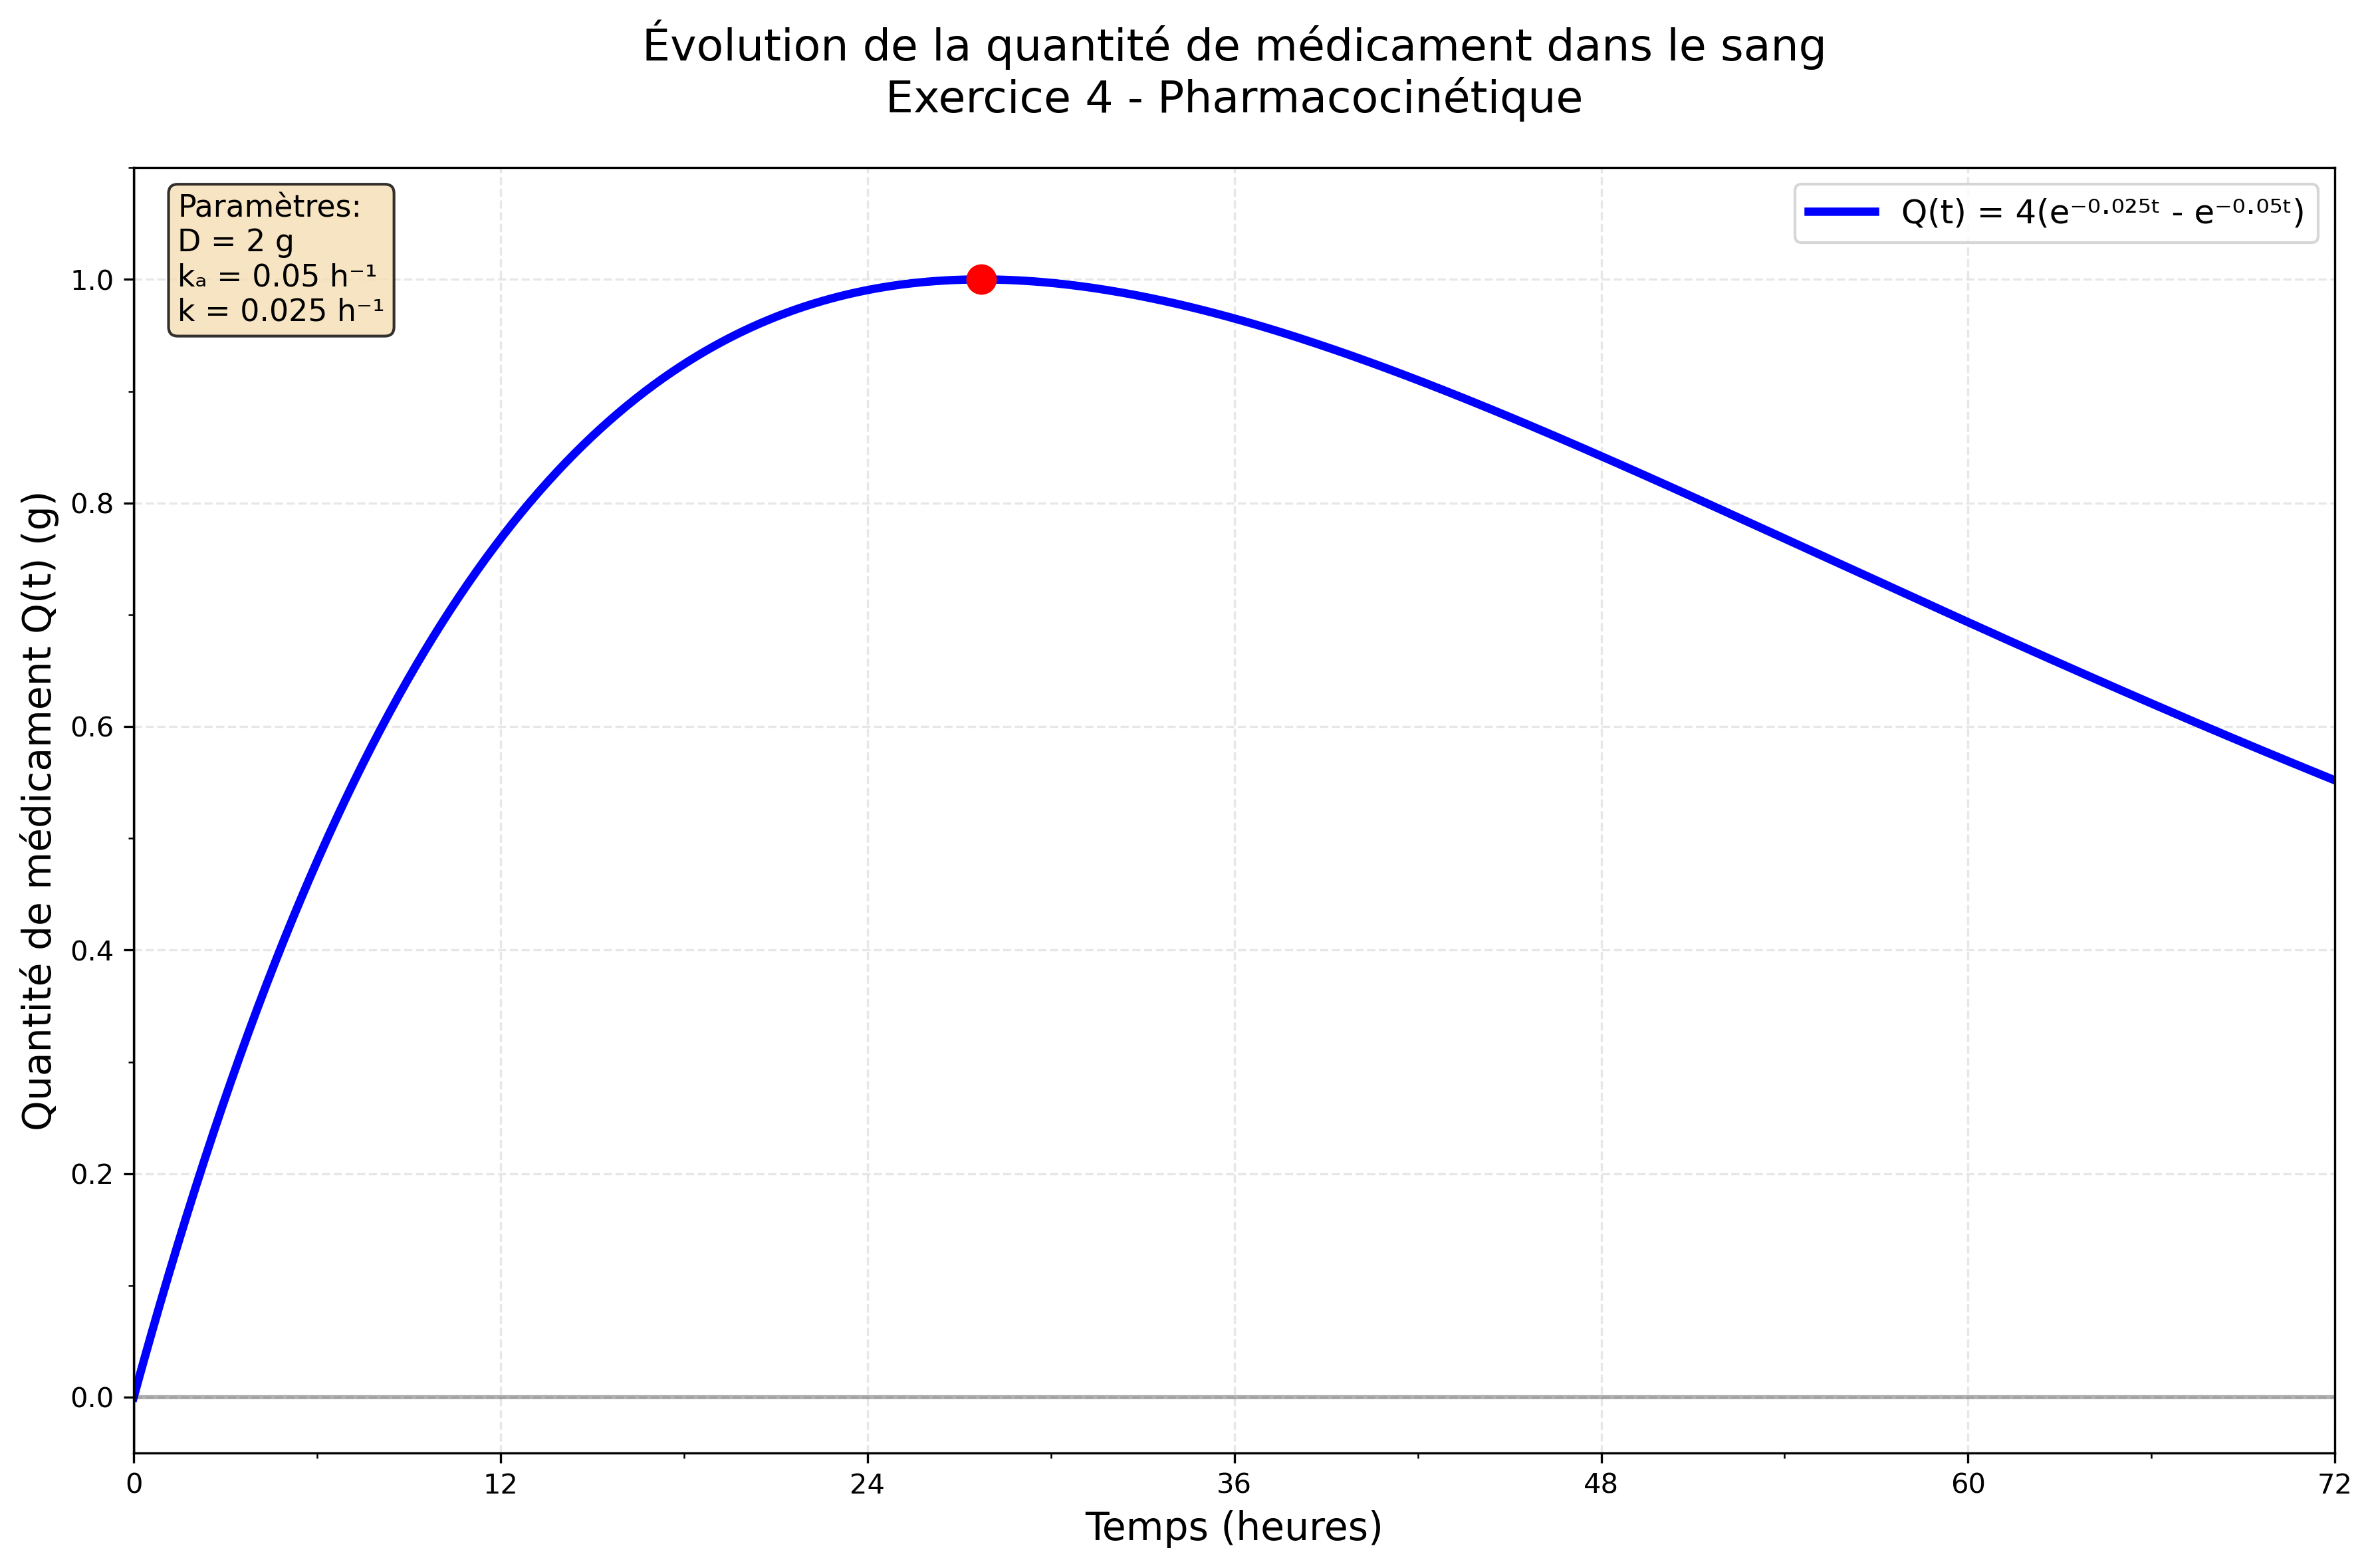
\includegraphics[width=0.6\textwidth]{images/courbe_pharmacocinetique.png}
\end{center}
\end{boitecorrige}


\newpage
\section{EDO du second ordre : méthodes avancées}

\subsection*{Exercice 16 - EDO du 2\textsuperscript{e} ordre : solution générale complète \niveau{\moyen}}

\begin{boiteexercice}
Résoudre les équations différentielles suivantes en trouvant la solution homogène et une solution particulière :
\begin{enumerate}[label=(\alph*)]
  \item $y'' + 3y' + 2y = 6\e^x$
  \item $y'' - 4y' + 4y = \e^{2x}$ (racine double au second membre)
  \item $y'' + 4y = 8\cos(2x)$ (résonance en cosinus)
  \item $y'' + 2y' + 5y = 10x\e^{-x}$ avec $y(0)=0$, $y'(0)=1$
\end{enumerate}
\end{boiteexercice}

\begin{boitecorrige}
\textbf{(a)} Équation caractéristique : $r^2+3r+2 = (r+1)(r+2) = 0$, racines $r_1=-1$, $r_2=-2$. Solution homogène : $y_h = C_1\e^{-x}+C_2\e^{-2x}$. Solution particulière $y_p = A\e^x$ (1 n'est pas racine) : $A+3A+2A = 6$, $A=1$.
\[
y = C_1\e^{-x} + C_2\e^{-2x} + \e^x
\]

\textbf{(b)} Racine double $r=2$. Solution homogène : $y_h = (C_1+C_2 x)\e^{2x}$.
Comme $r=2$ est racine double, on multiplie par $x^2$ : $y_p = Ax^2\e^{2x}$.
On calcule $y_p'' - 4y_p' + 4y_p = 2A\e^{2x} = \e^{2x}$, donc $A=1/2$.
\[
y = (C_1+C_2 x)\e^{2x} + \frac{x^2}{2}\e^{2x}
\]

\textbf{(c)} Homogène : $y_h = C_1\cos(2x)+C_2\sin(2x)$. Résonance : $y_p = x(A\cos(2x)+B\sin(2x))$.
On calcule $y_p''+4y_p = -4A\sin(2x)+4B\cos(2x) = 8\cos(2x)$, d'où $B=2$, $A=0$.
\[
y = C_1\cos(2x)+C_2\sin(2x)+2x\sin(2x)
\]

\textbf{(d)} Équation caractéristique : $r^2+2r+5=0$, racines $r=-1\pm 2j$. Solution homogène : $y_h = \e^{-x}(C_1\cos 2x+C_2\sin 2x)$. Solution particulière $y_p = \e^{-x}(Ax+B)$. On substitue : $y_p = \e^{-x}(Ax+B)$, $y_p' = \e^{-x}(A-Ax-B)$, $y_p'' = \e^{-x}(-2A+Ax+B)$. Donc $y_p''+2y_p'+5y_p = \e^{-x}(5Ax+5B) = 10x\e^{-x}$ : $A=2$, $B=0$.

Conditions initiales : $y(0) = C_1 = 0$, $y'(0) = -C_1+2C_2+2 = 1$, $C_2=-1/2$.
\[
y(x) = \e^{-x}\!\left(-\frac{1}{2}\sin 2x + 2x\right)
\]
\end{boitecorrige}

\subsection*{Exercice 17 - Variation des constantes pour $y'' + y = 1/\sin x$ \niveau{\difficile}}

\begin{boiteexercice}
Résoudre par la méthode de variation des constantes :
\[
y'' + y = \frac{1}{\sin x}, \quad x\in\,]0,\pi[
\]
\begin{enumerate}
  \item Trouver les deux solutions de l'équation homogène $y_1$ et $y_2$.
  \item Calculer le wronskien $W(y_1,y_2)$.
  \item Poser $y_p = C_1(x)y_1 + C_2(x)y_2$ et écrire le système pour $C_1'$ et $C_2'$.
  \item Intégrer et donner la solution particulière.
  \item Donner la solution générale.
\end{enumerate}
\end{boiteexercice}

\begin{boitecorrige}
\textbf{1.} L'équation homogène $y''+y=0$ a les racines $r=\pm j$ : $y_1 = \cos x$, $y_2 = \sin x$.

\textbf{2.} Wronskien : $W = y_1 y_2' - y_1' y_2 = \cos x\cos x - (-\sin x)\sin x = \cos^2 x + \sin^2 x = 1$.

\textbf{3.} Le système de variation des constantes est :
\[
C_1' y_1 + C_2' y_2 = 0, \quad C_1' y_1' + C_2' y_2' = \frac{1}{\sin x}
\]
D'où :
\[
C_1' = -\frac{y_2 f}{W} = -\frac{\sin x/\sin x}{1} = -1, \quad C_2' = \frac{y_1 f}{W} = \frac{\cos x/\sin x}{1} = \frac{\cos x}{\sin x}
\]

\textbf{4.} En intégrant :
\[
C_1 = -x, \quad C_2 = \int\frac{\cos x}{\sin x}\,\d x = \ln|\sin x| = \ln(\sin x) \quad\text{(car $x\in]0,\pi[$)}
\]
Solution particulière :
\[
y_p = -x\cos x + \sin x\ln(\sin x)
\]

\textbf{5.} Solution générale :
\[
\boxed{y = C_1\cos x + C_2\sin x - x\cos x + \sin x\ln(\sin x)}
\]
\end{boitecorrige}

\subsection*{Exercice 18 - Équation de Bessel d'ordre $n$ \niveau{\difficile}}

\begin{boiteexercice}
L'équation de Bessel d'ordre $n$ est :
\[
x^2 y'' + xy' + (x^2 - n^2)y = 0, \quad x > 0
\]
\begin{enumerate}
  \item Pour $n=0$, vérifier que la solution en série entière de la forme $y = \sum_{k=0}^\infty a_k x^{2k}$ ($a_0=1$) converge et calculer $a_1$ et $a_2$.
  \item On admet que les solutions régulières sont les fonctions de Bessel $J_n(x)$. Donner les premiers termes de $J_0(x)$ et $J_1(x)$.
  \item Pour le problème des modes propres d'une membrane circulaire de rayon $R$ (équation $\Delta u + k^2 u = 0$), les modes axiaux vérifient $J_0(k_{0n}R) = 0$. Calculer les 3 premiers zéros de $J_0$.
  \item La relation de récurrence $J_{n-1}(x)+J_{n+1}(x) = \frac{2n}{x}J_n(x)$ permet de calculer $J_n$ pour tout $n$. Calculer $J_2(1)$ sachant que $J_0(1)\approx0{,}765$ et $J_1(1)\approx0{,}440$.
\end{enumerate}
\end{boiteexercice}

\begin{boitecorrige}
\textbf{1.} Pour $n=0$, en substituant $y = \sum a_k x^{2k}$ dans $xy''+(y'+xy) = 0$... en fait dans $x^2 y''+xy'+x^2 y=0$, terme par terme :
\[
\sum_{k=0}^\infty\bigl[2k(2k-1)a_k x^{2k} + 2ka_k x^{2k} + a_{k-1}x^{2k}\bigr] = 0
\]
soit $(2k)^2 a_k + a_{k-1} = 0$, d'où $a_k = -a_{k-1}/(4k^2)$.

\[
a_0 = 1,\quad a_1 = -\frac{1}{4},\quad a_2 = \frac{1}{64},\quad a_3 = -\frac{1}{2304},\ldots
\]

\textbf{2.} Fonctions de Bessel :
\[
J_0(x) = 1 - \frac{x^2}{4} + \frac{x^4}{64} - \ldots = \sum_{k=0}^\infty \frac{(-1)^k}{(k!)^2}\left(\frac{x}{2}\right)^{2k}
\]
\[
J_1(x) = \frac{x}{2} - \frac{x^3}{16} + \ldots = \sum_{k=0}^\infty \frac{(-1)^k}{k!(k+1)!}\left(\frac{x}{2}\right)^{2k+1}
\]

\textbf{3.} Les trois premiers zéros de $J_0$ (tables) :
\[
z_{01}\approx 2{,}405,\quad z_{02}\approx 5{,}520,\quad z_{03}\approx 8{,}654
\]
Les fréquences propres sont $f_{0n} = c\, z_{0n}/(2\pi R)$ pour une membrane de rayon $R$.

\textbf{4.} Relation de récurrence pour $n=1$ :
\[
J_0(1) + J_2(1) = \frac{2}{1}J_1(1) \implies J_2(1) = 2J_1(1) - J_0(1)\approx 2\times0{,}440 - 0{,}765 = 0{,}115
\]
\end{boitecorrige}

\subsection*{Exercice 19 - Système d'EDO linéaire : résolution par valeurs propres \niveau{\difficile}}

\begin{boiteexercice}
On considère le système différentiel $\dot{X} = AX$ avec :
\[
A = \begin{pmatrix}0 & 1 \\ -2 & -3\end{pmatrix}
\]
\begin{enumerate}
  \item Calculer les valeurs propres et les vecteurs propres de $A$.
  \item En déduire la solution générale du système homogène.
  \item Résoudre le problème de Cauchy avec $X(0) = \begin{pmatrix}1\\0\end{pmatrix}$.
  \item Calculer l'exponentielle de matrice $\e^{At}$ et vérifier que $X(t) = \e^{At}X(0)$.
  \item Étudier le comportement asymptotique : vers quel état le système tend-il pour $t\to+\infty$ ?
\end{enumerate}
\end{boiteexercice}

\begin{boitecorrige}
\textbf{1.} Équation caractéristique : $\lambda^2+3\lambda+2 = (\lambda+1)(\lambda+2) = 0$, d'où $\lambda_1=-1$ et $\lambda_2=-2$.

Vecteur propre pour $\lambda_1=-1$ : $(A+I)v_1 = 0$ donne $\begin{pmatrix}1&1\\-2&-2\end{pmatrix}v_1=0$, soit $v_1 = \begin{pmatrix}1\\-1\end{pmatrix}$.

Vecteur propre pour $\lambda_2=-2$ : $(A+2I)v_2 = 0$ donne $v_2 = \begin{pmatrix}1\\-2\end{pmatrix}$.

\textbf{2.} Solution générale :
\[
X(t) = C_1\begin{pmatrix}1\\-1\end{pmatrix}\e^{-t} + C_2\begin{pmatrix}1\\-2\end{pmatrix}\e^{-2t}
\]

\textbf{3.} Conditions initiales $X(0) = \begin{pmatrix}1\\0\end{pmatrix}$ :
\[
C_1+C_2 = 1, \quad -C_1-2C_2 = 0 \implies C_1 = 2,\; C_2 = -1
\]
\[
X(t) = \begin{pmatrix}2\e^{-t}-\e^{-2t}\\-2\e^{-t}+2\e^{-2t}\end{pmatrix}
\]

\textbf{4.} La matrice fondamentale est $\Phi(t) = \begin{pmatrix}\e^{-t}&\e^{-2t}\\-\e^{-t}&-2\e^{-2t}\end{pmatrix}$ et $\e^{At} = \Phi(t)\Phi(0)^{-1}$.

$\Phi(0)^{-1} = \begin{pmatrix}2&1\\-1&-1\end{pmatrix}$, donc :
\[
\e^{At} = \begin{pmatrix}2\e^{-t}-\e^{-2t} & \e^{-t}-\e^{-2t}\\-2\e^{-t}+2\e^{-2t} & -\e^{-t}+2\e^{-2t}\end{pmatrix}
\]

\textbf{5.} Pour $t\to+\infty$ : les deux valeurs propres sont négatives ($\lambda_1=-1$, $\lambda_2=-2$), donc $X(t)\to\vec{0}$. L'origine est un \textbf{n\oe{}ud stable} : toutes les trajectoires convergent vers l'équilibre $X=0$.
\end{boitecorrige}

\subsection*{Exercice 20 - Équation de Legendre et polynômes de Legendre \niveau{\difficile}}

\begin{boiteexercice}
L'équation de Legendre est :
\[
(1-x^2)y'' - 2xy' + n(n+1)y = 0, \quad x\in[-1,1]
\]
\begin{enumerate}
  \item Montrer que $x=0$ est un point ordinaire et chercher une solution en série $y = \sum_{k=0}^\infty a_k x^k$.
  \item Montrer que les coefficients vérifient $a_{k+2} = -\frac{(n-k)(n+k+1)}{(k+2)(k+1)}a_k$.
  \item Pour $n=2$, en partant de $a_0=1$, $a_1=0$, calculer $P_2(x)$.
  \item Vérifier que $P_2(x) = \frac{1}{2}(3x^2-1)$ est bien solution.
  \item La condition d'orthogonalité est $\int_{-1}^1 P_m(x)P_n(x)\,\d x = \frac{2}{2n+1}\delta_{mn}$. Vérifier pour $m=0$, $n=2$.
\end{enumerate}
\end{boiteexercice}

\begin{boitecorrige}
\textbf{1.} En $x=0$, les coefficients sont $p(x)=-2x/(1-x^2)$ et $q(x)=n(n+1)/(1-x^2)$, continus en $x=0$ : point ordinaire. En substituant $y = \sum a_k x^k$ dans l'équation :
\[
(1-x^2)\sum_{k=2}^\infty k(k-1)a_k x^{k-2} - 2x\sum_{k=1}^\infty ka_k x^{k-1} + n(n+1)\sum a_k x^k = 0
\]

\textbf{2.} En collectant les termes en $x^k$ :
\[
(k+2)(k+1)a_{k+2} - k(k-1)a_k - 2ka_k + n(n+1)a_k = 0
\]
\[
a_{k+2} = \frac{k(k+1)-n(n+1)}{(k+2)(k+1)}a_k = -\frac{(n-k)(n+k+1)}{(k+2)(k+1)}a_k
\]

\textbf{3.} Pour $n=2$, $a_0=1$, $a_1=0$ :
\[
a_2 = -\frac{(2-0)(2+1)}{2\cdot1}a_0 = -3, \quad a_4 = -\frac{(2-2)(2+3)}{4\cdot3}a_2 = 0
\]
Donc la série est finie : $y = 1 - 3x^2$. Le polynôme normalisé est $P_2(x) = \frac{1}{2}(3x^2-1)$ (avec $a_0 = -1/2$ pour la normalisation standard $P_n(1)=1$).

\textbf{4.} Vérification : $P_2 = \frac{3x^2-1}{2}$, $P_2' = 3x$, $P_2'' = 3$.
\[
(1-x^2)\cdot3 - 2x\cdot3x + 2\cdot3\cdot\frac{3x^2-1}{2} = 3-3x^2-6x^2+9x^2-3 = 0\quad
\]

\textbf{5.} $P_0(x)=1$ et $P_2(x) = \frac{3x^2-1}{2}$ :
\[
\int_{-1}^1 P_0 P_2\,\d x = \int_{-1}^1\frac{3x^2-1}{2}\,\d x = \frac{1}{2}\left[x^3-x\right]_{-1}^1 = \frac{1}{2}(1-1-(-1+1)) = 0 = \delta_{02}\quad
\]
\end{boitecorrige}

\subsection*{Exercice 21 - Transformation de Laplace pour les EDO \niveau{\moyen}}

\begin{boiteexercice}
Rappel : $\mathcal{L}\{y'\} = sY(s)-y(0)$, $\mathcal{L}\{y''\} = s^2Y(s)-sy(0)-y'(0)$, $\mathcal{L}\{\e^{at}\} = 1/(s-a)$.

Résoudre par la transformée de Laplace :
\begin{enumerate}
  \item $y''+y = \sin t$ avec $y(0)=0$, $y'(0)=0$.
  \item $y''+4y'+4y = \e^{-2t}$ avec $y(0)=0$, $y'(0)=1$.
  \item $y''-y = \e^t + 1$ avec $y(0)=0$, $y'(0)=0$.
\end{enumerate}
\end{boiteexercice}

\begin{boitecorrige}
\textbf{1.} Transformée : $(s^2+1)Y = \mathcal{L}\{\sin t\} = 1/(s^2+1)$, donc $Y = 1/(s^2+1)^2$.

Décomposition partielle : $\mathcal{L}^{-1}\{1/(s^2+1)^2\} = \frac{1}{2}(\sin t - t\cos t)$.
\[
\boxed{y = \frac{1}{2}(\sin t - t\cos t)}
\]

\textbf{2.} Transformée (conditions $y(0)=0$, $y'(0)=1$) :
\[
(s^2+4s+4)Y - 1 = \frac{1}{s+2}
\]
\[
Y = \frac{1}{(s+2)^2} + \frac{1}{(s+2)^3}
\]
Inversée : $\mathcal{L}^{-1}\{1/(s+2)^2\} = t\e^{-2t}$, $\mathcal{L}^{-1}\{1/(s+2)^3\} = \frac{t^2}{2}\e^{-2t}$.
\[
y = t\e^{-2t} + \frac{t^2}{2}\e^{-2t} = \left(t+\frac{t^2}{2}\right)\e^{-2t}
\]

\textbf{3.} Transformée :
\[
(s^2-1)Y = \frac{1}{s-1} + \frac{1}{s} = \frac{s+s-1}{s(s-1)}
\]
\[
Y = \frac{2s-1}{s(s-1)(s+1)(s-1)} = \frac{2s-1}{s(s-1)^2(s+1)}
\]
Par fractions partielles : $Y = \frac{1}{s} + \frac{A}{s-1} + \frac{B}{(s-1)^2} + \frac{C}{s+1}$.

$s=0$ : $\frac{-1}{1\cdot(-1)} = 1$. $s\to\infty$ : A+C+1=0. $s=-1$ : $C = \frac{-3}{(-2)^2} = -3/4$. $s=1$ : $B = 1/2$. $A = -1/4$.
\[
y(t) = 1 - \frac{1}{4}\e^t + \frac{t}{2}\e^t - \frac{3}{4}\e^{-t} = 1 + \frac{2t-1}{4}\e^t - \frac{3}{4}\e^{-t}
\]
\end{boitecorrige}

\subsection*{Exercice 22 - Système proie-prédateur (Lotka-Volterra) \niveau{\difficile}}

\begin{boiteexercice}
On considère le système différentiel de Lotka-Volterra décrivant l'évolution couplée des populations de proies $x(t)$ et de prédateurs $y(t)$ :
\[
\dot x = ax - bxy, \qquad \dot y = -cy + dxy
\]
avec $a, b, c, d > 0$.
\begin{enumerate}
  \item Interpréter physiquement chaque terme.
  \item Trouver les points d'équilibre.
  \item Montrer que la quantité $H(x,y) = dx - c\ln x + by - a\ln y$ est conservée.
  \item Décrire qualitativement les trajectoires dans le plan de phase.
\end{enumerate}
\end{boiteexercice}

\begin{boitecorrige}
\textbf{1.} $ax$ : croissance naturelle des proies. $-bxy$ : mortalité due aux prédateurs. $-cy$ : mortalité naturelle des prédateurs. $+dxy$ : croissance des prédateurs proportionnelle aux proies consommées.

\textbf{2.} Points d'équilibre ($\dot x = \dot y = 0$) :
\[
(x, y) = (0, 0) \quad\text{ou}\quad (x^*, y^*) = (c/d, a/b)
\]

\textbf{3.} Dérivons $H$ le long des trajectoires :
\[
\frac{\d H}{\d t} = d\dot x - c\frac{\dot x}{x} + b\dot y - a\frac{\dot y}{y}
= \dot x\!\left(d - \frac{c}{x}\right) + \dot y\!\left(b - \frac{a}{y}\right)
\]
\[
= (ax - bxy)\frac{dx-c}{x} + (-cy+dxy)\frac{by-a}{y} = (a-by)(dx-c) - (c-dx)(a-by) = 0
\]
Donc $H$ est conservée : les trajectoires sont des courbes de niveau de $H$.

\textbf{4.} Les trajectoires sont des courbes fermées autour du point d'équilibre non trivial $(c/d, a/b)$ : les populations oscillent périodiquement (cycles proie-prédateur). Quand les proies abondent, les prédateurs prolifèrent, puis les proies diminuent, entraînant le déclin des prédateurs, et le cycle recommence.
\reponse{Équilibre $(c/d, a/b)$ ; $H(x,y) = dx - c\ln x + by - a\ln y$ conservée ; trajectoires fermées.}
\end{boitecorrige}

\subsection*{Exercice 23 - Équation de la chaleur 1D par séparation des variables \niveau{\difficile}}

\begin{boiteexercice}
On cherche à résoudre l'équation de la chaleur sur $[0, L]$ :
\[
\frac{\partial u}{\partial t} = D\frac{\partial^2 u}{\partial x^2}, \qquad u(0,t) = u(L,t) = 0, \quad u(x, 0) = f(x)
\]
\begin{enumerate}
  \item Chercher des solutions de la forme $u(x,t) = X(x)T(t)$ et établir les équations séparées.
  \item Déterminer les modes spatiaux $X_n(x)$ et temporels $T_n(t)$.
  \item Donner la solution générale.
  \item Pour $f(x) = u_0\sin(\pi x/L)$, donner la solution explicite.
\end{enumerate}
\end{boiteexercice}

\begin{boitecorrige}
\textbf{1.} $X T' = D X'' T$ soit $T'/T = D X''/X = -\lambda D$ (constante). D'où :
\[
X'' + (\lambda/D) X = 0, \qquad T' + \lambda T = 0
\]
(avec $\lambda > 0$ pour avoir décroissance temporelle)

\textbf{2.} Conditions aux limites $X(0) = X(L) = 0$ imposent $\lambda_n = D(n\pi/L)^2$ :
\[
X_n(x) = \sin\!\left(\frac{n\pi x}{L}\right), \qquad T_n(t) = \e^{-n^2\pi^2 D t/L^2}
\]

\textbf{3.} Solution générale (série de Fourier) :
\[
u(x,t) = \sum_{n=1}^\infty b_n \sin\!\left(\frac{n\pi x}{L}\right) \e^{-n^2\pi^2 D t/L^2}
\]
avec $b_n = \dfrac{2}{L}\displaystyle\int_0^L f(x)\sin\!\left(\dfrac{n\pi x}{L}\right)\d x$.

\textbf{4.} Pour $f(x) = u_0\sin(\pi x/L)$ : un seul mode $b_1 = u_0$, tous les autres $b_n = 0$ ($n\geq 2$).
\[
u(x,t) = u_0\sin\!\left(\frac{\pi x}{L}\right)\e^{-\pi^2 D t/L^2}
\]
Le profil spatial est conservé, l'amplitude décroît en exponentielle, avec constante de temps
\[
\tau = \frac{L^2}{\pi^2 D}.
\]
\reponse{$u(x,t) = \sum b_n \sin(n\pi x/L)\e^{-n^2\pi^2 Dt/L^2}$}
\end{boitecorrige}

\subsection*{Exercice 24 - Méthode d'Euler pour $\dot y = y$ \niveau{\facile}}

\begin{boiteexercice}
On considère l'EDO $\dot y = y$ avec $y(0) = 1$. La solution exacte est $y(t) = \e^t$.
\begin{enumerate}
  \item Rappeler le schéma d'Euler explicite de pas $h$.
  \item Calculer $y_1, y_2, y_3$ pour $h = 0{,}1$.
  \item Comparer avec les valeurs exactes.
  \item Donner l'erreur relative à $t = 0{,}3$.
\end{enumerate}
\end{boiteexercice}

\begin{boitecorrige}
\textbf{1.} Schéma d'Euler explicite :
\[
y_{n+1} = y_n + h\,f(t_n, y_n) = y_n(1 + h)
\]
(puisque $f(t,y) = y$).

\textbf{2.} Avec $h = 0{,}1$, $y_0 = 1$ :
\[
y_1 = 1{,}1, \quad y_2 = 1{,}21, \quad y_3 = 1{,}331
\]

\textbf{3.} Valeurs exactes : $\e^{0{,}1} \approx 1{,}1052$, $\e^{0{,}2} \approx 1{,}2214$, $\e^{0{,}3} \approx 1{,}3499$.

\textbf{4.} Erreur relative à $t = 0{,}3$ :
\[
\varepsilon = \frac{|1{,}331 - 1{,}3499|}{1{,}3499} \approx 1{,}4\,\%
\]
L'erreur locale à chaque pas est $O(h^2)$, l'erreur globale est $O(h)$.
\reponse{$y_3 \approx 1{,}331$ vs $\e^{0{,}3} \approx 1{,}3499$ ; erreur relative $\approx 1{,}4\,\%$.}
\end{boitecorrige}

\subsection*{Exercice 25 - Stabilité d'un schéma numérique \niveau{\moyen}}

\begin{boiteexercice}
On résout $\dot y = -\lambda y$ ($\lambda > 0$) par Euler explicite avec pas $h$.
\begin{enumerate}
  \item Donner la relation de récurrence.
  \item Étudier la stabilité : pour quelle condition sur $h$ la solution numérique reste-t-elle bornée ?
  \item Application : pour $\lambda = 10$, quel pas maximal garantit la stabilité ?
  \item Comparer avec le schéma d'Euler implicite.
\end{enumerate}
\end{boiteexercice}

\begin{boitecorrige}
\textbf{1.} $y_{n+1} = y_n - h\lambda y_n = (1 - h\lambda)\,y_n$, soit $y_n = (1 - h\lambda)^n y_0$.

\textbf{2.} Stabilité : $|y_n|$ doit rester bornée quand $n\to\infty$, soit $|1 - h\lambda| \leq 1$ :
\[
-1 \leq 1 - h\lambda \leq 1 \iff 0 \leq h\lambda \leq 2
\]
Condition de stabilité : $\boxed{h \leq 2/\lambda}$.

\textbf{3.} Pour $\lambda = 10$ : $h_\text{max} = 2/10 = 0{,}2$. Au-delà, la solution numérique oscille et diverge.

\textbf{4.} Schéma implicite : $y_{n+1} = y_n - h\lambda y_{n+1}$, soit $y_{n+1} = \dfrac{y_n}{1 + h\lambda}$. Quel que soit $h > 0$, $|1/(1+h\lambda)| < 1$ : schéma \textbf{inconditionnellement stable}. C'est l'avantage principal des schémas implicites pour les équations raides.
\reponse{Euler explicite : $h \leq 2/\lambda$ ; pour $\lambda=10$, $h_\text{max} = 0{,}2$. Euler implicite : stable $\forall h > 0$.}
\end{boitecorrige}

\newpage
\section*{Galerie d'illustrations - Équations différentielles}

\begin{figure}[H]
\centering
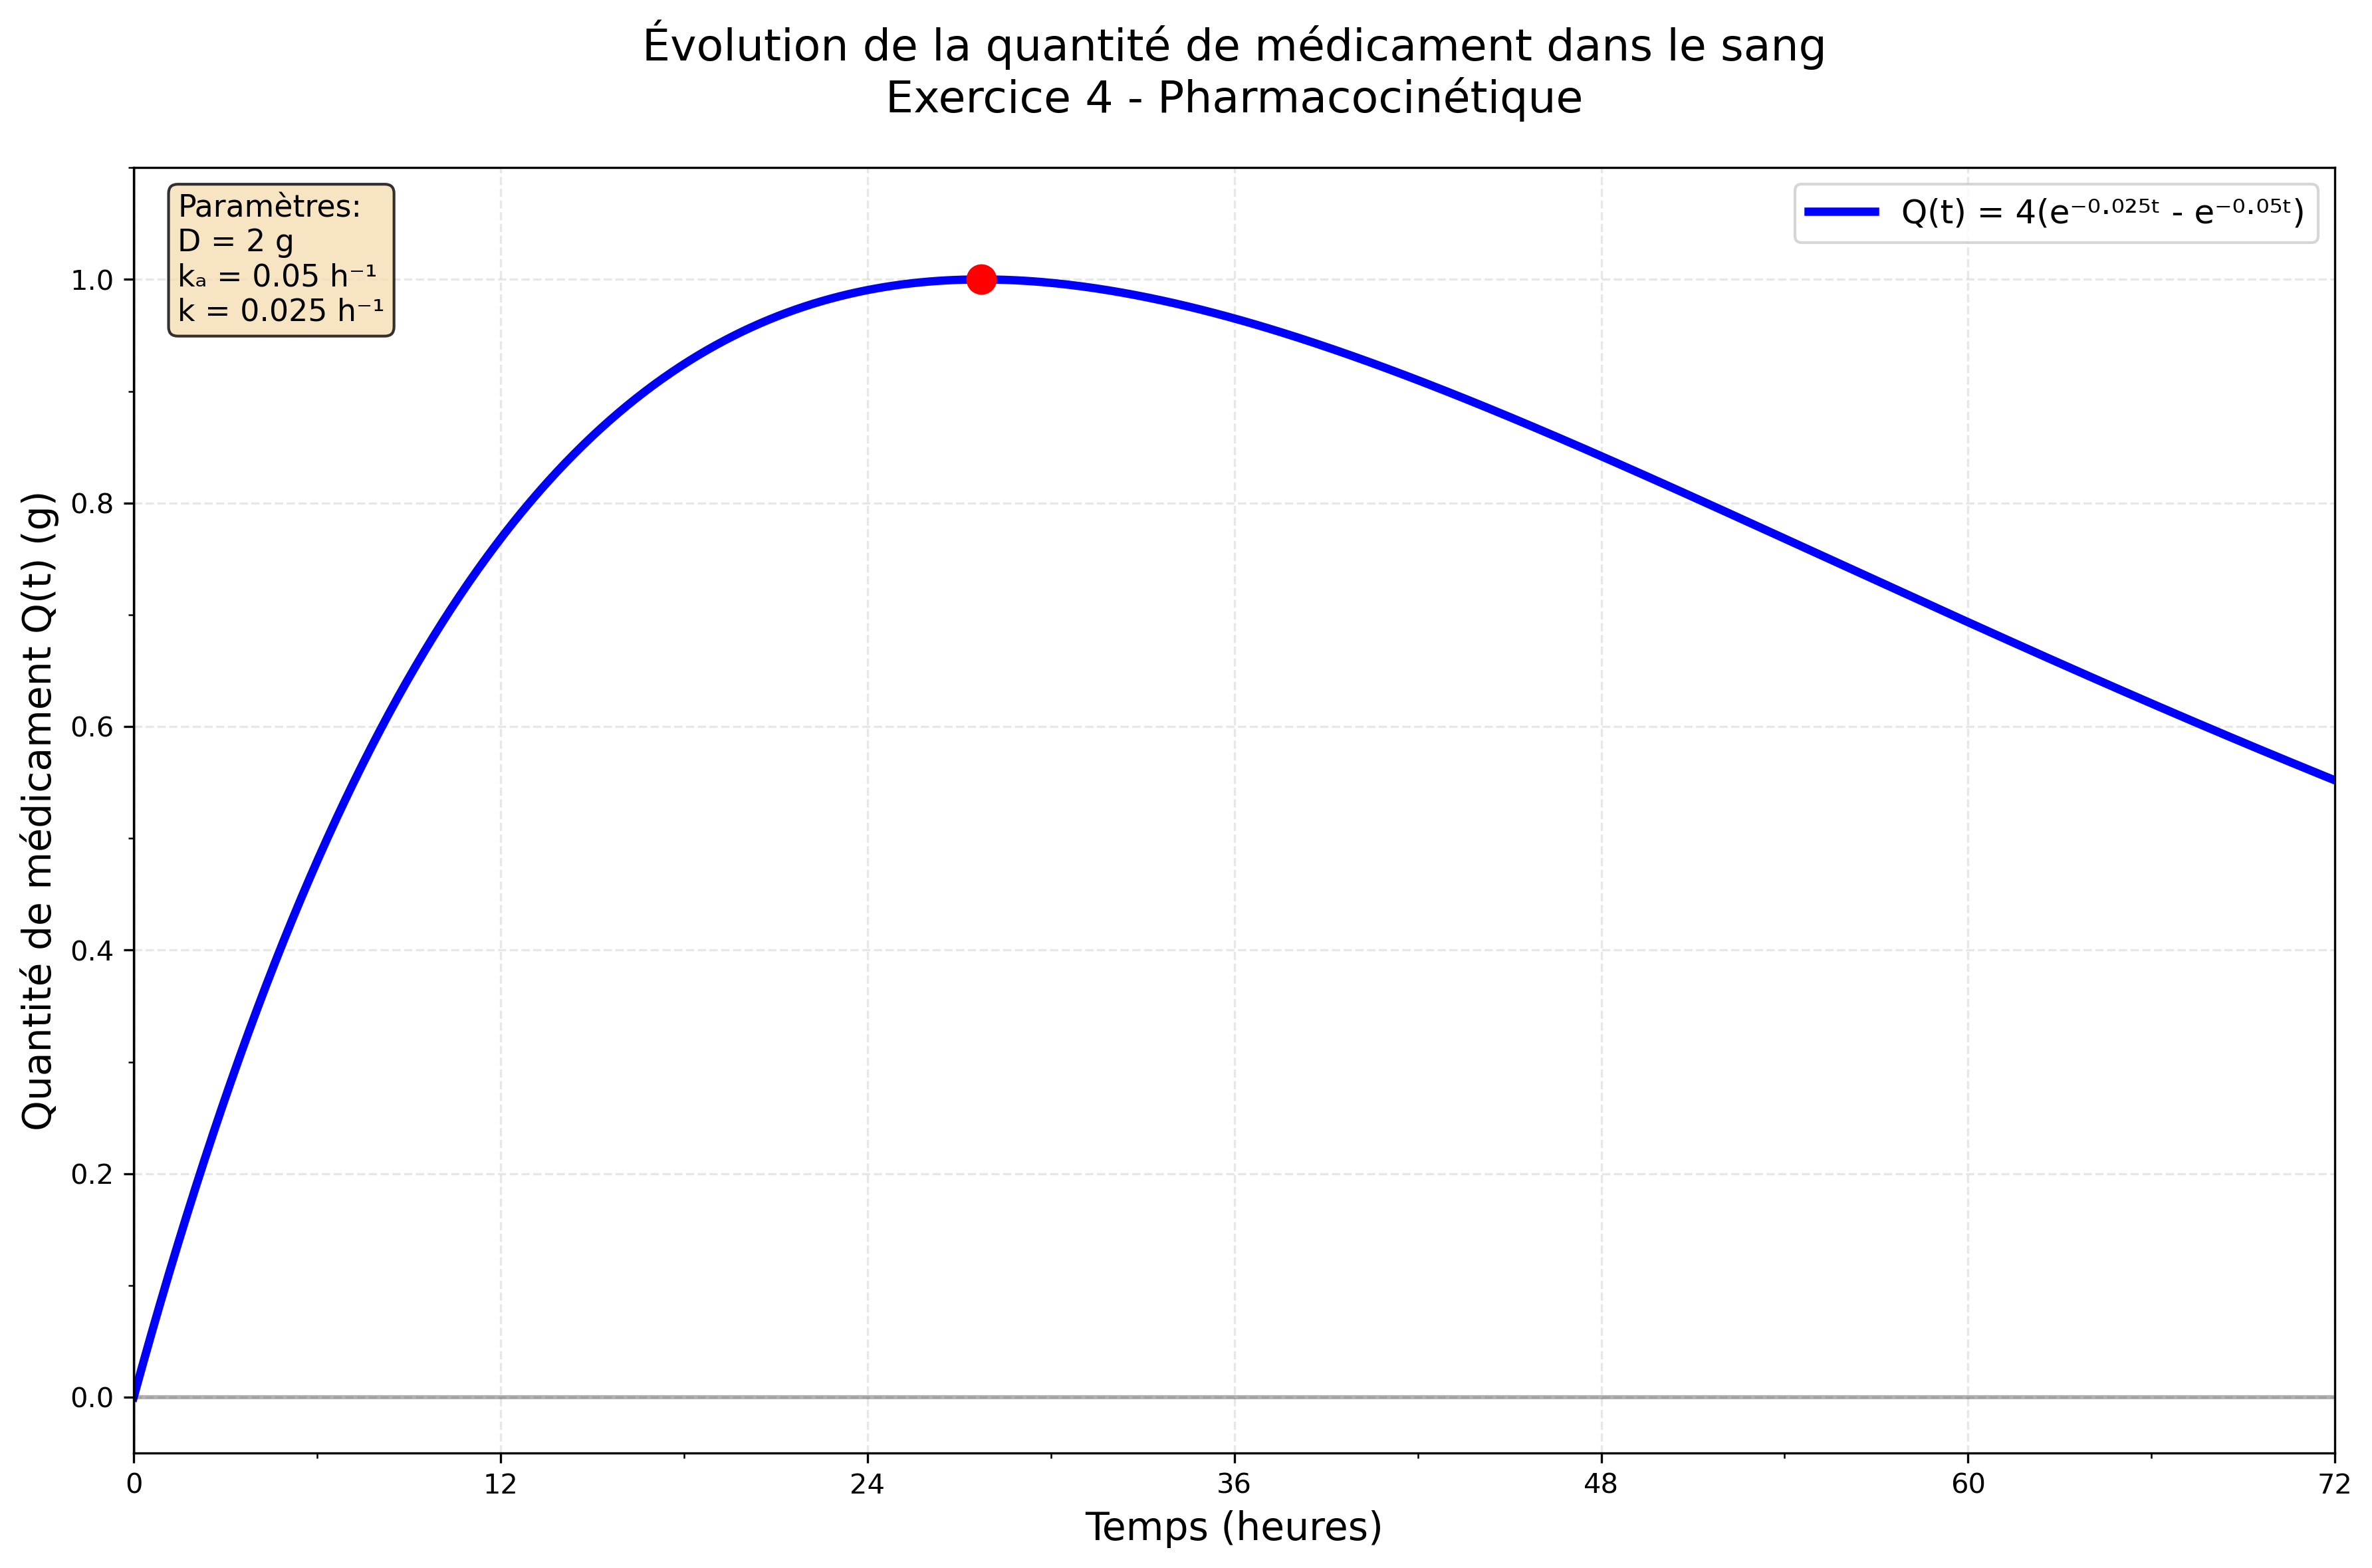
\includegraphics[width=0.7\textwidth]{images/edp/edo-028-000.png}
\caption{Résolution graphique d'une EDO.}
\end{figure}

\begin{figure}[H]
\centering

\includegraphics[width=0.7\textwidth]{images/edp/edo-028-001.png}
\caption{Champ de vecteurs et trajectoires.}
\end{figure}

\ifdefined\inMainDoc\else\end{document}\fi


% ================================================================
%  UE 3 : PHYSIQUE NUCLÉAIRE
% ================================================================
\newpage
\thispagestyle{empty}
\begin{tikzpicture}[remember picture, overlay]
  \fill[gray!12] ([xshift=1.5cm, yshift=3cm]current page.south west)
    rectangle ([xshift=-1.5cm, yshift=-3cm]current page.north east);
  \draw[line width=3pt] ([xshift=1.5cm,yshift=-3cm]current page.north west)
    -- ([xshift=-1.5cm,yshift=-3cm]current page.north east);
  \draw[line width=3pt] ([xshift=1.5cm,yshift=3cm]current page.south west)
    -- ([xshift=-1.5cm,yshift=3cm]current page.south east);
  \node[align=center] at (current page.center) {%
    {\fontsize{34}{42}\bfseries\selectfont PHYSIQUE NUCLÉAIRE}\\[1.2cm]
    {\large\itshape Structure du noyau - Radioactivité}\\[0.4cm]
    {\large\itshape Réactions nucléaires - Fission et fusion}\\[1.8cm]
    {\normalsize Licence 3 - UE 3}
  };
  \node[anchor=south west] at ([xshift=2cm,yshift=2cm]current page.south west)
    {\large\bfseries UE 3};
\end{tikzpicture}
\newpage

\addcontentsline{toc}{section}{PHYSIQUE NUCLÉAIRE}
\ifdefined\inMainDoc\else
\documentclass[12pt,a4paper]{article}
% ================================================================
%  PRÉAMBULE COMMUN - ANNALES CORRIGÉES
%  Université de Kara - FaST - Licence Fondamentale MPC
%  Design optimisé impression noir et blanc
% ================================================================

% -- ENCODAGE & LANGUE --
\usepackage[utf8]{inputenc}
\usepackage[T1]{fontenc}
\usepackage[french]{babel}
\usepackage{lmodern}
\usepackage{microtype}

% -- MISE EN PAGE --
\usepackage[a4paper, top=2.8cm, bottom=2.5cm, left=2.5cm, right=2.5cm, headheight=14pt]{geometry}
\usepackage{setspace}
\setstretch{1.2}
\usepackage{parskip}
\setlength{\parindent}{1.2em}
\setlength{\parskip}{4pt}

% -- MATHS --
\usepackage{amsmath, amssymb, mathtools, amsthm}
\usepackage{mathrsfs}
\usepackage{dsfont}
\usepackage{bm}
\usepackage{cancel}
\usepackage{textcomp}
% Définition de \oiint (intégrale de surface fermée) sans package supplémentaire
\newcommand{\oiint}{\mathop{\iint\!\!\!\!\!\!\!\bigcirc}\limits}

% -- PHYSIQUE & CHIMIE --
\usepackage{physics}
\usepackage{siunitx}
% Lorsque physics est chargé, siunitx omet \qty. On le restaure ici :
\AtBeginDocument{\RenewCommandCopy\qty\SI}
\sisetup{locale = FR, detect-all, output-decimal-marker={,}}
% Commande de substitution pour les unités posant problème avec pdflatex
% (ohm, degreeCelsius, micro, angstrom, percent utilisent des caractères non-ASCII)
\newcommand{\qtyohm}[1]{\ensuremath{\num{#1}\,\Omega}}
\newcommand{\qtydegc}[1]{\ensuremath{\num{#1}\,{}^\circ\text{C}}}
\newcommand{\qtyangstrom}[1]{\ensuremath{\num{#1}\,\text{\AA}}}
\newcommand{\qtypercent}[1]{\ensuremath{\num{#1}\,\%}}
\newcommand{\qtyum}[1]{\ensuremath{\num{#1}\,\mu\text{m}}}
\usepackage[version=4]{mhchem}

% -- GRAPHISMES --
\usepackage{graphicx}
\usepackage{float}
\usepackage{caption}
\usepackage{subcaption}
\usepackage{wrapfig}
\usepackage{tikz}
\usetikzlibrary{calc, arrows.meta, patterns, shapes.geometric}
\usepackage{pgfplots}
\pgfplotsset{compat=1.18}

% -- TABLEAUX --
\usepackage{booktabs}
\usepackage{array}
\usepackage{tabularx}
\usepackage{multirow}

% -- LISTES --
\usepackage{enumitem}
\setlist[enumerate]{topsep=3pt, itemsep=2pt, parsep=0pt}
\setlist[itemize]{topsep=3pt, itemsep=2pt, parsep=0pt, label={.}}

% -- BOÎTES (noir et blanc) --
\usepackage{mdframed}
\usepackage{tcolorbox}
\tcbuselibrary{skins, breakable, theorems}

% Boîte EXERCICE : encadré avec filet épais, fond blanc
\newmdenv[
  linewidth=1.2pt,
  linecolor=black,
  roundcorner=3pt,
  skipabove=10pt,
  skipbelow=6pt,
  innertopmargin=8pt,
  innerbottommargin=8pt,
  innerleftmargin=10pt,
  innerrightmargin=10pt,
  backgroundcolor=white,
  frametitle={\bfseries\small Exercice},
  frametitlealignment=\raggedright,
  frametitleaboveskip=4pt,
  frametitlebelowskip=4pt,
]{boiteexercice}

% Boîte CORRIGÉ : fond gris très clair + filet fin
\newmdenv[
  linewidth=0.6pt,
  linecolor=black,
  leftline=true,
  rightline=false,
  topline=false,
  bottomline=false,
  linecolor=black,
  innerleftmargin=12pt,
  innerrightmargin=8pt,
  innertopmargin=6pt,
  innerbottommargin=6pt,
  backgroundcolor=gray!8,
  skipabove=4pt,
  skipbelow=8pt,
]{boitecorrige}

% Boîte RÉSUMÉ DE COURS : double encadré
\newmdenv[
  linewidth=0.8pt,
  linecolor=black,
  roundcorner=2pt,
  backgroundcolor=gray!12,
  innertopmargin=10pt,
  innerbottommargin=10pt,
  innerleftmargin=12pt,
  innerrightmargin=12pt,
  skipabove=12pt,
  skipbelow=8pt,
]{boiteresume}

% Boîte ATTENTION/REMARQUE : barre gauche épaisse
\newmdenv[
  leftline=true,
  rightline=false,
  topline=false,
  bottomline=false,
  linewidth=3pt,
  linecolor=black,
  backgroundcolor=gray!5,
  innerleftmargin=12pt,
  innerrightmargin=8pt,
  innertopmargin=5pt,
  innerbottommargin=5pt,
  skipabove=6pt,
  skipbelow=6pt,
]{boiteremarque}

% -- DIFFICULTÉ DES EXERCICES --
\newcommand{\facile}{$\star$}
\newcommand{\moyen}{$\star\!\star$}
\newcommand{\difficile}{$\star\!\star\!\star$}
\newcommand{\niveau}[1]{\hfill\textbf{#1}\hspace{2pt}}

% -- EN-TÊTES ET PIEDS DE PAGE --
\usepackage{fancyhdr}
\pagestyle{fancy}
\fancyhf{}
\renewcommand{\headrulewidth}{0.5pt}
\renewcommand{\footrulewidth}{0.3pt}

% -- HYPERLIENS --
\usepackage[hidelinks]{hyperref}
\hypersetup{
    colorlinks=false,
    pdftitle={Annale Corrigée - Licence MPC - Université de Kara}
}

% -- TITRES --
\usepackage{titlesec}
\titleformat{\section}{\Large\bfseries}{\thesection.}{0.8em}{}[\vspace{2pt}\hrule\vspace{4pt}]
\titleformat{\subsection}{\large\bfseries}{\thesubsection.}{0.7em}{}
\titleformat{\subsubsection}{\normalsize\bfseries}{\thesubsubsection.}{0.6em}{}

% -- THÉORÈMES --
\theoremstyle{definition}
\newtheorem{defn}{Définition}[section]
\newtheorem{prop}{Propriété}[section]
\newtheorem{thm}{Théorème}[section]
\newtheorem{corol}{Corollaire}[section]
\newtheorem{exemple}{Exemple}[section]

% -- COMMANDES MATHÉMATIQUES UTILES --
\newcommand{\vect}[1]{\overrightarrow{#1}}
\newcommand{\R}{\mathbb{R}}
\newcommand{\N}{\mathbb{N}}
\newcommand{\Z}{\mathbb{Z}}
\newcommand{\C}{\mathbb{C}}
\renewcommand{\d}{\mathrm{d}}
\newcommand{\deriv}[2]{\dfrac{\d #1}{\d #2}}
\newcommand{\dpart}[2]{\dfrac{\partial #1}{\partial #2}}
\newcommand{\rot}{\overrightarrow{\mathrm{rot}}\,}
\renewcommand{\div}{\mathrm{div}\,}
\renewcommand{\grad}{\overrightarrow{\mathrm{grad}}\,}
\newcommand{\e}{\mathrm{e}}
\newcommand{\ii}{\mathrm{i}}
\renewcommand{\Tr}{\mathrm{Tr}}

% Numérotation des équations par section
\numberwithin{equation}{section}

% -- RÉSULTATS ENCADRÉS --
\newcommand{\res}[1]{\[\boxed{#1}\]}

% -- REMARQUE INLINE --
\newcommand{\rmq}[1]{\begin{boiteremarque}\textbf{Remarque.} #1\end{boiteremarque}}

% -- MISE EN VALEUR DU RÉSULTAT FINAL --
\newcommand{\reponse}[1]{%
  \begin{center}
    \fbox{\begin{minipage}{0.92\textwidth}\centering #1\end{minipage}}
  \end{center}%
}


\lhead{\small\textit{Physique Nucléaire - Licence 3}}
\rhead{\small\textit{FaST, Université de Kara}}
\cfoot{\thepage}

\begin{document}
\fi

\begin{center}
  {\LARGE\bfseries PHYSIQUE NUCLÉAIRE ET RADIOACTIVITÉ}\\[0.3cm]
  {\normalsize Licence 3 - Physique}\\[0.1cm]
  \rule{0.7\textwidth}{0.8pt}
\end{center}

\section*{Résumé du cours}

\begin{boiteresume}

\textbf{1. Structure du noyau.} Un noyau ${}^A_Z$X contient $Z$ protons et $N = A-Z$ neutrons. La masse du noyau est inférieure à la somme des masses de ses constituants : c'est le défaut de masse $\Delta m = Zm_p + Nm_n - m_{noyau}$. L'énergie de liaison est $E_L = \Delta m\cdot c^2$.

\textbf{2. Loi de désintégration radioactive.} À chaque instant, un échantillon de $N$ noyaux radioactifs se désintègre à un taux proportionnel à $N$ :
\[
\frac{\d N}{\d t} = -\lambda N \quad \Rightarrow \quad N(t) = N_0\,\e^{-\lambda t}
\]
La constante $\lambda$ est la constante de désintégration. La demi-vie $t_{1/2} = \ln 2/\lambda$ est le temps au bout duquel la moitié des noyaux s'est désintégrée.

\textbf{3. Activité.} $A(t) = \lambda N(t) = A_0\,\e^{-\lambda t}$, en Becquerel (Bq $=$ \unit{s^{-1}}).

\textbf{4. Types de désintégrations.}
\begin{itemize}[nosep]
  \item $\alpha$ : émission d'un noyau d'hélium ${}^4_2$He. ${}^A_Z$X $\to$ ${}^{A-4}_{Z-2}$Y $+ {}^4_2$He.
  \item $\beta^-$ : émission d'un électron et un antineutrino. ${}^A_Z$X $\to$ ${}^A_{Z+1}$Y $+ \bar{\nu}_e + e^-$.
  \item $\gamma$ : émission d'un photon de haute énergie (désexcitation du noyau).
\end{itemize}

\end{boiteresume}

\newpage
\section{Radioactivité}

\subsection*{Exercice 1 - Loi de désintégration \niveau{\facile}}

\begin{boiteexercice}
Le carbone 14 a une demi-vie $t_{1/2} = \qty{5730}{ans}$. Un échantillon de bois vivant contient $N_0 = \qty{6.5e10}{}$ atomes de ${}^{14}$C par gramme de carbone.
\begin{enumerate}
  \item Calculer la constante de désintégration $\lambda$.
  \item Quelle est l'activité initiale de l'échantillon par gramme de carbone ?
  \item Un fossile contient $3{,}25\times10^{10}$ atomes de ${}^{14}$C par gramme. Quel est son âge ?
\end{enumerate}
\end{boiteexercice}

\begin{boitecorrige}
\textbf{1.} $\lambda = \ln2/t_{1/2} = 0{,}6931/(5730\times365{,}25\times24\times3600) = \qty{3.83e-12}{s^{-1}}$.

\textbf{2.} $A_0 = \lambda N_0 = 3{,}83\times10^{-12}\times6{,}5\times10^{10} \approx \qty{0.249}{Bq.g^{-1}}$.

\textbf{3.} $N(t) = N_0\,\e^{-\lambda t}$. On cherche $t$ tel que $N(t)/N_0 = 3{,}25/6{,}5 = 0{,}5 = \e^{-\lambda t}$. Donc $\lambda t = \ln 2$, soit $t = t_{1/2} = \qty{5730}{ans}$.
\end{boitecorrige}

\subsection*{Exercice 2 - Désintégrations successives \niveau{\moyen}}

\begin{boiteexercice}
L'uranium 238 ($t_{1/2} = \qty{4.47e9}{ans}$) se désintègre en une chaîne de plusieurs radionucléides, dont le radon 222 ($t_{1/2} = \qty{3.82}{jours}$) qui se désintègre lui-même en polonium 218 ($t_{1/2} = \qty{3.05}{min}$).

\begin{enumerate}
  \item Écrire les équations de désintégration pour ${}^{222}_{86}$Rn $\to$ ${}^{218}_{84}$Po.
  \item Un échantillon contient initialement $N_0 = 10^{10}$ atomes de Rn-222. Calculer $N_{\text{Rn}}(t)$ et l'activité $A_{\text{Rn}}(t)$ à $t = \qty{7.64}{jours}$.
  \item Que peut-on dire du régime d'équilibre radioactif entre Rn-222 et Po-218 après suffisamment de temps ?
\end{enumerate}
\end{boiteexercice}

\begin{boitecorrige}
\textbf{1.} La désintégration du radon en polonium est une désintégration $\alpha$ :
\[
{}^{222}_{86}\text{Rn} \longrightarrow {}^{218}_{84}\text{Po} + {}^4_2\text{He}
\]

\textbf{2.} $t = \qty{7.64}{jours} = 2t_{1/2}(\text{Rn})$. $N_{\text{Rn}}(t) = N_0\,\e^{-\lambda_{\text{Rn}}t} = N_0\times(1/2)^2 = 2{,}5\times10^9$ atomes.

$\lambda_{\text{Rn}} = \ln2/(3{,}82\times86400) = \qty{2.1e-6}{s^{-1}}$.
$A_{\text{Rn}} = \lambda_{\text{Rn}}\times N_{\text{Rn}} = 2{,}1\times10^{-6}\times2{,}5\times10^9 \approx \qty{5250}{Bq}$.

\textbf{3.} Puisque $t_{1/2}(\text{Po-218}) \ll t_{1/2}(\text{Rn-222})$, le Po-218 se crée et se désintègre bien plus vite qu'il ne s'accumule. Après un temps de l'ordre de quelques $t_{1/2}(\text{Po})$, l'équilibre séculaire est atteint : $A_{\text{Po}} = A_{\text{Rn}}$ (les activités s'égalisent).
\end{boitecorrige}

\subsection*{Exercice 3 - Énergie de liaison \niveau{\moyen}}

\begin{boiteexercice}
Calculer l'énergie de liaison et l'énergie de liaison par nucléon du noyau ${}^{56}_{26}$Fe (fer-56).

\textbf{Données :} $m({}^{56}_{26}\text{Fe}) = \qty{55.9349}{u}$, $m_p = \qty{1.007276}{u}$, $m_n = \qty{1.008665}{u}$, $\qty{1}{u} = \qty{931.5}{MeV.c^{-2}}$.
\end{boiteexercice}

\begin{boitecorrige}
Le noyau de ${}^{56}$Fe contient $Z=26$ protons et $N=56-26=30$ neutrons.

Défaut de masse :
\[
\Delta m = 26\times1{,}007276 + 30\times1{,}008665 - 55{,}9349
\]
\[
= 26{,}189176 + 30{,}25995 - 55{,}9349 = 0{,}515126\,\text{u}
\]

Énergie de liaison :
\[
E_L = \Delta m\times931{,}5 = 0{,}515126\times931{,}5 \approx \qty{480}{MeV}
\]

Énergie de liaison par nucléon :
\[
\frac{E_L}{A} = \frac{480}{56} \approx \qty{8.57}{MeV.nucl^{-1}}
\]
Le fer-56 est l'un des noyaux les plus stables de la nature (maximum de la courbe d'Aston).
\end{boitecorrige}


\newpage
\section{Radioactivité et désintégration}

\subsection*{Exercice 4 - Loi de désintégration radioactive \niveau{\moyen}}

\begin{boiteexercice}
Un échantillon radioactif contient initialement $N_0 = 10^{12}$ noyaux. La période (demi-vie) est $T_{1/2} = 5730$ ans (carbone-14).
\begin{enumerate}
  \item Écrire la loi de désintégration et calculer la constante radioactive $\lambda$.
  \item Calculer l'activité initiale $A_0$.
  \item Combien de noyaux reste-t-il après $t = 10000$ ans ?
  \item Quelle est l'activité après 10000 ans ?
\end{enumerate}
\end{boiteexercice}

\begin{boitecorrige}
\textbf{1.} Loi de désintégration : $N(t) = N_0\,\e^{-\lambda t}$.

Constante radioactive : $\lambda = \dfrac{\ln 2}{T_{1/2}} = \dfrac{0{,}693}{5730\,\text{ans}} = 1{,}21\times10^{-4}\,\text{ans}^{-1}$.

En convertissant : $\lambda = \dfrac{1{,}21\times10^{-4}}{3{,}156\times10^7\,\text{s}} = 3{,}83\times10^{-12}\,\text{s}^{-1}$.

\textbf{2.} Activité initiale :
\[
A_0 = \lambda N_0 = 3{,}83\times10^{-12} \times 10^{12} = 3{,}83\,\text{désintégrations/s} = 3{,}83\,\text{Bq}
\]

\textbf{3.} Nombre de noyaux après $t = 10000$ ans :
\[
N(10000) = 10^{12}\times\e^{-1{,}21\times10^{-4}\times10000} = 10^{12}\times\e^{-1{,}21} \approx 2{,}98\times10^{11}
\]

\textbf{4.} Activité après 10000 ans :
\[
A(10000) = \lambda N(10000) = 3{,}83\times10^{-12}\times2{,}98\times10^{11} \approx 1{,}14\,\text{Bq}
\]
\end{boitecorrige}

\subsection*{Exercice 5 - Formule de Bethe-Weizsäcker \niveau{\difficile}}

\begin{boiteexercice}
La formule de Bethe-Weizsäcker exprime l'énergie de liaison des noyaux :
\[
E_L(A,Z) = a_v A - a_s A^{2/3} - a_c \frac{Z(Z-1)}{A^{1/3}} - a_a\frac{(A-2Z)^2}{A} + \delta(A,Z)
\]
avec $a_v = 15{,}5\;\text{MeV}$, $a_s = 17{,}2\;\text{MeV}$, $a_c = 0{,}72\;\text{MeV}$, $a_a = 23\;\text{MeV}$.
\begin{enumerate}
  \item Expliquer la signification physique de chaque terme.
  \item Calculer $E_L$ pour ${}^{56}_{26}$Fe en utilisant cette formule ($\delta=0$) et comparer avec la valeur expérimentale $E_L^{exp} \approx 492\;\text{MeV}$.
  \item Montrer que le numéro atomique optimal $Z_{opt}$ minimisant l'énergie totale est :
  \[
  Z_{opt} = \frac{A}{2 + a_c A^{2/3}/(2a_a)}
  \]
\end{enumerate}
\end{boiteexercice}

\begin{boitecorrige}
\textbf{1.} Signification des termes :
\begin{itemize}[nosep]
  \item $a_v A$ : terme de volume (interaction forte, proportionnel au volume du noyau)
  \item $-a_s A^{2/3}$ : terme de surface (nucléons en surface moins liés)
  \item $-a_c Z(Z-1)/A^{1/3}$ : terme coulombien (répulsion entre protons)
  \item $-a_a(A-2Z)^2/A$ : terme d'asymétrie (favorise $N=Z$)
  \item $\delta$ : terme d'appariement (noyaux pair-pair plus stables)
\end{itemize}

\textbf{2.} Pour ${}^{56}$Fe ($A=56$, $Z=26$, $N=30$) :
\begin{align*}
E_v &= 15{,}5 \times 56 = 868\;\text{MeV} \\
E_s &= -17{,}2 \times 56^{2/3} = -17{,}2 \times 14{,}42 = -247{,}9\;\text{MeV} \\
E_c &= -0{,}72 \times \frac{26\times25}{56^{1/3}} = -0{,}72\times\frac{650}{3{,}83} = -122{,}1\;\text{MeV} \\
E_a &= -23 \times \frac{(56-52)^2}{56} = -23\times\frac{16}{56} = -6{,}57\;\text{MeV}
\end{align*}
\[
E_L \approx 868 - 247{,}9 - 122{,}1 - 6{,}57 \approx 491{,}4\;\text{MeV}
\]
Très bonne concordance avec $E_L^{exp} \approx 492\;\text{MeV}$.

\textbf{3.} En minimisant $E_L$ par rapport à $Z$ (en traitant $E_c \approx -a_c Z^2/A^{1/3}$) :
\[
\frac{\partial E_L}{\partial Z} = -\frac{2a_c Z}{A^{1/3}} + \frac{4a_a(A-2Z)}{A} = 0
\]
\[
Z\left(\frac{2a_c}{A^{1/3}} + \frac{8a_a}{A}\right) = \frac{4a_a A}{A} = 4a_a
\]
\[
Z_{opt} = \frac{4a_a}{\frac{2a_c}{A^{1/3}} + \frac{8a_a}{A}} = \frac{A}{2 + \frac{a_c A^{2/3}}{2a_a}}
\]
\end{boitecorrige}

\subsection*{Exercice 6 - Fission et fusion nucléaire \niveau{\moyen}}

\begin{boiteexercice}
\begin{enumerate}
  \item La fission de l'uranium-235 : ${}^{235}_{92}\text{U} + n \to {}^{141}_{56}\text{Ba} + {}^{92}_{36}\text{Kr} + 3n$. Calculer l'énergie libérée, sachant que :
  $m({}^{235}\text{U}) = 235{,}044\;\text{u}$, $m({}^{141}\text{Ba}) = 140{,}914\;\text{u}$, $m({}^{92}\text{Kr}) = 91{,}926\;\text{u}$, $m_n = 1{,}009\;\text{u}$.
  \item La fusion deutérium-tritium : ${}^2_1\text{H} + {}^3_1\text{H} \to {}^4_2\text{He} + n$. Sachant que $Q = 17{,}6\;\text{MeV}$, expliquer pourquoi cette réaction est difficile à réaliser.
  \item Comparer les énergies libérées par nucléon pour les deux processus.
\end{enumerate}
\end{boiteexercice}

\begin{boitecorrige}
\textbf{1.} Défaut de masse :
\[
\Delta m = m({}^{235}\text{U}) + m_n - m({}^{141}\text{Ba}) - m({}^{92}\text{Kr}) - 3m_n
\]
\[
= 235{,}044 + 1{,}009 - 140{,}914 - 91{,}926 - 3\times1{,}009 = 0{,}195\;\text{u}
\]
\[
Q = 0{,}195\times931{,}5 \approx 181{,}6\;\text{MeV}
\]

\textbf{2.} La réaction D-T libère $Q=17{,}6\;\text{MeV}$ mais nécessite de vaincre la barrière coulombienne entre les deux noyaux chargés positivement. La température requise est $T \sim 10^8\;\text{K}$ (plasma de fusion). C'est le défi de la fusion thermonucléaire contrôlée.

\textbf{3.} Énergie par nucléon :
\begin{itemize}[nosep]
  \item Fission : $Q/A = 181{,}6/236 \approx 0{,}77\;\text{MeV/nucléon}$
  \item Fusion D-T : $Q/(2+3) = 17{,}6/5 = 3{,}52\;\text{MeV/nucléon}$
\end{itemize}
La fusion libère environ 4-5 fois plus d'énergie par nucléon que la fission.
\end{boitecorrige}

\subsection*{Exercice 7 - Réactions nucléaires : Q-valeur \niveau{\moyen}}

\begin{boiteexercice}
Pour la réaction ${}^4_2\text{He} + {}^{14}_7\text{N} \to {}^{17}_8\text{O} + {}^1_1\text{H}$, calculer :
\begin{enumerate}
  \item La Q-valeur (en utilisant les masses atomiques).
  \item L'énergie cinétique minimale du projectile $\alpha$ pour que la réaction soit possible (énergie de seuil).
\end{enumerate}
Données : $m({}^4\text{He}) = 4{,}0026\;\text{u}$, $m({}^{14}\text{N}) = 14{,}0031\;\text{u}$, $m({}^{17}\text{O}) = 16{,}9991\;\text{u}$, $m({}^1\text{H}) = 1{,}0078\;\text{u}$.
\end{boiteexercice}

\begin{boitecorrige}
\textbf{1.} Q-valeur :
\begin{align*}
Q &= \bigl[m({}^4\text{He}) + m({}^{14}\text{N}) - m({}^{17}\text{O}) - m({}^1\text{H})\bigr]\times931{,}5\;\text{MeV/u} \\
&= (4{,}0026 + 14{,}0031 - 16{,}9991 - 1{,}0078)\times931{,}5 \\
&= (-0{,}0012)\times931{,}5 \approx -1{,}12\;\text{MeV}
\end{align*}
Comme $Q < 0$, la réaction est endothermique.

\textbf{2.} L'énergie de seuil (en référentiel du laboratoire, cible ${}^{14}$N au repos) :
\[
T_{seuil} = |Q|\cdot\frac{m_\alpha + m_N + m_O + m_H}{2m_N} \approx |Q|\cdot\frac{A_{total}}{2A_{cible}} = 1{,}12\times\frac{36}{28} \approx 1{,}44\;\text{MeV}
\]
\end{boitecorrige}


\newpage
\section{Exercices complémentaires de radioactivité}

\subsection*{Exercice 8 - Volume sanguin par traceur radioactif (Thallium) \niveau{\moyen}}

\begin{boiteexercice}
On injecte dans le sang d'un patient une solution de ${}_{81}^{199}$Tl d'activité $A_0 = 960\;\text{kBq}$. La demi-vie du Tl-199 est de 7,5 heures. 15 heures après l'injection, on mesure l'activité $A'$ d'un prélèvement de volume $V' = 10\;\text{mL}$ : on obtient 480 Bq.
\begin{enumerate}
  \item Comment est définie l'activité d'un échantillon radioactif ? Quelle est son unité ?
  \item Pourquoi l'activité diminue-t-elle au cours du temps ?
  \item Définir la demi-vie.
  \item Calculer l'activité résiduelle $A_1$ de la totalité de la solution dans le sang 15 heures après l'injection.
  \item Pourquoi $A'$ est-il différent de $A_1$ ?
  \item Déduire le volume total de sang dans le corps humain.
  \item ${}_{81}^{199}$Tl est radioactif $\beta^+$. Écrire l'équation de désintégration.
\end{enumerate}
\end{boiteexercice}

\begin{boitecorrige}
\textbf{1.} L'activité est le nombre de désintégrations radioactives par seconde. Unité : Becquerel (Bq).

\textbf{2.} L'activité est proportionnelle au nombre de noyaux radioactifs présents, qui diminue à chaque désintégration.

\textbf{3.} La demi-vie est la durée nécessaire pour que la moitié des noyaux radioactifs se désintègrent.

\textbf{4.} 15 heures $= 2 \times t_{1/2}$, donc $A_1 = A_0/4 = 960/4 = 240\;\text{kBq}$.

\textbf{5.} $A'$ et $A_1$ sont mesurées au même instant, mais sur des volumes différents : $V' = 10\;\text{mL}$ contre le volume total $V_1$.

\textbf{6.} À un instant donné, l'activité est proportionnelle au volume : $\dfrac{A_1}{A'} = \dfrac{V_1}{V'}$, donc $V_1 = \dfrac{A_1}{A'}\times V' = \dfrac{240\times10^3}{480}\times10 = 5000\;\text{mL} = \qty{5}{L}$.

\textbf{7.} Radioactivité $\beta^+$ (excès de protons) : ${}_{81}^{199}\text{Tl} \rightarrow {}_{80}^{199}\text{Hg} + {}_{+1}^{0}\beta^+ + \nu_e$.
\end{boitecorrige}

\subsection*{Exercice 9 - Modèle analogique de la désintégration (dés) \niveau{\facile}}

\begin{boiteexercice}
On modélise la désintégration radioactive avec un lot de 100 dés dodécaédriques (12 faces). Une face est peinte en blanc, les autres en noir. À chaque lancer, les dés montrant la face blanche sont éliminés.
\begin{enumerate}
  \item Quelle est la probabilité d'obtenir la face blanche ? La face noire ?
  \item Compléter le tableau de l'évolution du nombre de dés :
  \begin{center}
  \begin{tabular}{|l|c|c|c|c|c|c|c|c|}
  \hline
  Lancers & 0 & 1 & 2 & 3 & 4 & 5 & 6 & 7 \\
  \hline
  Dés restants & 100 & 92 & 84 & 77 & 71 & 65 & 60 & 55 \\
  \hline
  \end{tabular}
  \end{center}
  \item Quelle est l'analogie avec la radioactivité ?
\end{enumerate}
\end{boiteexercice}

\begin{boitecorrige}
\textbf{1.} $P(\text{blanc}) = 1/12$, $P(\text{noir}) = 11/12$.

\textbf{2.} À chaque lancer, il reste $11/12$ des dés. On passe d'une case à la suivante en multipliant par $11/12$.

\textbf{3.} Un dé montrant la face blanche représente un noyau radioactif qui se désintègre. Un lancer représente un intervalle de temps pendant lequel une fraction $1/12$ des noyaux se désintègre. La décroissance est exponentielle, similaire à la loi $N(t) = N_0\,\mathrm{e}^{-\lambda t}$.
\end{boitecorrige}

\subsection*{Exercice 10 - Chaîne de désintégration du Radium \niveau{\moyen}}

\begin{boiteexercice}
Le radium ${}_{88}^{226}$Ra se transforme en plomb stable ${}_{82}^{206}$Pb par une série de désintégrations $\alpha$ et $\beta^-$.
\begin{enumerate}
  \item Donner la composition du noyau de ${}_{88}^{226}$Ra.
  \item Définir les désintégrations $\alpha$ et $\beta^-$. Comment $A$ et $Z$ varient-ils ?
  \item Écrire l'équation de la première désintégration (type $\alpha$, produit : radon Rn).
  \item Le radon est lui-même radioactif $\beta^-$ et donne un isotope du francium Fr. Écrire l'équation.
  \item Déterminer le nombre de désintégrations $\alpha$ et $\beta^-$ nécessaires pour passer de Ra à Pb.
\end{enumerate}
\end{boiteexercice}

\begin{boitecorrige}
\textbf{1.} ${}_{88}^{226}$Ra : 88 protons et $226-88 = 138$ neutrons.

\textbf{2.} Désintégration $\alpha$ : émission de ${}_{2}^{4}$He, $A$ diminue de 4, $Z$ diminue de 2. Désintégration $\beta^-$ : émission d'un électron, $A$ inchangé, $Z$ augmente de 1.

\textbf{3.} ${}_{88}^{226}\text{Ra} \rightarrow {}_{86}^{222}\text{Rn} + {}_{2}^{4}\text{He}$.

\textbf{4.} ${}_{86}^{222}\text{Rn} \rightarrow {}_{87}^{222}\text{Fr} + {}_{-1}^{0}e^- + \bar{\nu}_e$.

\textbf{5.} De Ra à Pb : $\Delta A = 226-206 = 20 \Rightarrow 20/4 = 5$ désintégrations $\alpha$. Ces 5 désintégrations $\alpha$ diminuent $Z$ de 10 ; or $\Delta Z = 88-82 = 6$ seulement. Il faut donc $10 - 6 = 4$ désintégrations $\beta^-$ pour compenser : \textbf{5 désintégrations $\alpha$ et 4 désintégrations $\beta^-$}.
\end{boitecorrige}

\subsection*{Exercice 11 - Énergie de liaison du carbone 12 \niveau{\moyen}}

\begin{boiteexercice}
La masse du noyau de ${}_{6}^{12}$C est $m = 1{,}9926\times10^{-26}\;\text{kg}$. On donne $m_p = 1{,}6726\times10^{-27}\;\text{kg}$, $m_n = 1{,}6749\times10^{-27}\;\text{kg}$, $c_0 = 2{,}998\times10^8\;\text{m.s}^{-1}$, $1\;\text{MeV} = 1{,}602\times10^{-13}\;\text{J}$.
\begin{enumerate}
  \item Calculer la masse de 6 protons et 6 neutrons séparés.
  \item Comparer à la masse du noyau. Expliquer la différence.
  \item Définir l'énergie de liaison.
  \item Calculer l'énergie de liaison en J puis en MeV. En déduire l'énergie de liaison par nucléon.
\end{enumerate}
\end{boiteexercice}

\begin{boitecorrige}
\textbf{1.} $m_\text{séparés} = 6\times1{,}6726\times10^{-27} + 6\times1{,}6749\times10^{-27} = 2{,}0085\times10^{-26}\;\text{kg}$.

\textbf{2.} $m_\text{séparés} > m_\text{noyau}$ : le noyau est plus léger que ses constituants séparés. La différence s'explique par la libération d'énergie lors de la formation du noyau (énergie de liaison).

\textbf{3.} L'énergie de liaison est l'énergie nécessaire pour décomposer le noyau en ses nucléons séparés.

\textbf{4.} $|\Delta m| = 2{,}0085\times10^{-26} - 1{,}9926\times10^{-26} = 1{,}59\times10^{-28}\;\text{kg}$.
\[
E_l = |\Delta m|c^2 = 1{,}59\times10^{-28}\times(2{,}998\times10^8)^2 = 1{,}43\times10^{-11}\;\text{J} \approx \qty{89.2}{MeV}
\]
Énergie de liaison par nucléon : $E_l/A = 89{,}2/12 \approx \qty{7.43}{MeV/nucléon}$.
\end{boitecorrige}

\subsection*{Exercice 12 - Centrale nucléaire : bilan énergétique \niveau{\difficile}}

\begin{boiteexercice}
On considère la fission de l'uranium 235 par un neutron, qui produit du baryum 141 et du krypton, ainsi que 3 neutrons. Le combustible nucléaire classique contient 5\,\% d'U-235 et 90\,\% d'U-238.
\begin{enumerate}
  \item Qu'est-ce que la radioactivité ?
  \item Quel mécanisme de transformation est utilisé dans les centrales nucléaires ?
  \item Écrire l'équation de la fission de ${}_{92}^{235}$U en ${}_{56}^{141}$Ba et Kr avec 3 neutrons.
  \item Calculer l'énergie libérée lors de cette fission (en J et en MeV).\\
    Masses : $m({}^{235}\text{U}) = 3{,}9043\times10^{-25}$ kg, $m({}^{141}\text{Ba}) = 2{,}3340\times10^{-25}$ kg, $m({}^{92}\text{Kr}) = 1{,}5262\times10^{-25}$ kg, $m_n = 1{,}6749\times10^{-28}$ kg.
  \item Calculer l'énergie libérée par 1 kg d'U-235 pur.
  \item Écrire l'équation de la transformation de ${}_{92}^{238}$U en ${}_{94}^{239}$Pu (enrichissement neutronique suivi de 2 désintégrations $\beta^-$).
  \item Le plutonium-239 se transforme en uranium-235 par désintégration $\alpha$. Écrire l'équation.
  \item Calculer l'énergie libérée par 1 kg de combustible classique.
\end{enumerate}
\end{boiteexercice}

\begin{boitecorrige}
\textbf{1.} La radioactivité est la transformation spontanée et aléatoire d'un noyau instable en un noyau plus stable, avec émission de rayonnements.

\textbf{2.} La fission provoquée : un neutron lent déclenche la fission d'un noyau lourd d'U-235.

\textbf{3.}
\[
{}_{92}^{235}\text{U} + {}_{0}^{1}n \rightarrow {}_{56}^{141}\text{Ba} + {}_{36}^{92}\text{Kr} + 3\,{}_{0}^{1}n
\]
Vérification : $235+1 = 141+92+3$ (nucléons) ; $92 = 56+36$ (charges).

\textbf{4.} Défaut de masse :
\begin{align*}
\Delta m &= \{m({}^{141}\text{Ba}) + m({}^{92}\text{Kr}) + 3m_n\} - \{m({}^{235}\text{U}) + m_n\}\\
&= \{2{,}3340 + 1{,}5262 + 3\times0{,}016749\} - \{3{,}9043 + 0{,}016749\} \approx -1{,}106\times10^{-27}\;\text{kg}
\end{align*}
\[
\Delta E = |\Delta m|c^2 = 1{,}106\times10^{-27}\times(3\times10^8)^2 \approx 9{,}95\times10^{-11}\;\text{J} \approx \qty{596}{MeV}
\]

\textbf{5.} Nombre d'atomes dans 1 kg : $N = 1/(3{,}9043\times10^{-25}) = 2{,}56\times10^{24}$.
\[
E(1\;\text{kg U-235}) = 596\times10^6\;\text{eV}\times2{,}56\times10^{24}\times1{,}6\times10^{-19}\;\text{J/eV} \approx \qty{2.45e14}{J} = \qty{245}{TJ}
\]

\textbf{6.} L'U-238 capture un neutron puis subit deux désintégrations $\beta^-$ :
\[
{}_{92}^{238}\text{U} + n \rightarrow {}_{93}^{239}\text{Np} + e^- + \bar{\nu}_e \rightarrow {}_{94}^{239}\text{Pu} + e^- + \bar{\nu}_e
\]

\textbf{7.} ${}_{94}^{239}\text{Pu} \rightarrow {}_{92}^{235}\text{U} + {}_{2}^{4}\text{He}$.

\textbf{8.} L'U-238 produit finalement de l'U-235 fissile avec bilan énergétique $596 - 29{,}2 \approx 567\;\text{MeV}$ par atome. Pour 1 kg de combustible (5\,\% U-235, 90\,\% U-238) :
\[
E(1\;\text{kg combustible}) \approx 0{,}05\times245 + 0{,}90\times230 \approx \qty{219}{TJ}
\]
\end{boitecorrige}


\subsection*{Exercice 13 - Désintégration radioactive du carbone-14 \niveau{\moyen}}

\begin{boiteexercice}
Le ${}^{14}$C se désintègre par émission $\beta^-$ avec une demi-vie $T_{1/2}=5730\;\text{ans}$.
\begin{enumerate}
  \item Donner la loi de décroissance $N(t)$ et l'expression de la constante $\lambda$ en fonction de $T_{1/2}$.
  \item Un fragment de bois archéologique présente une activité $A_\text{éch}=4\;\text{dps/g}$. L'activité d'un bois vivant est $A_0=13{,}6\;\text{dps/g}$. Calculer l'âge de l'échantillon.
  \item Calculer l'activité initiale (en Bq) de 1 g d'échantillon en supposant $N_0$ atomes de ${}^{14}$C pour 1 g ($N_0 = A_0/\lambda$).
  \item Quelle fraction de ${}^{14}$C reste-il après 3 demi-vies ?
\end{enumerate}
\end{boiteexercice}

\begin{boitecorrige}
\textbf{1.} La loi de décroissance radioactive :
\[
N(t) = N_0\,\e^{-\lambda t}, \qquad \lambda = \frac{\ln 2}{T_{1/2}}
\]
L'activité $A(t) = \lambda N(t) = A_0\,\e^{-\lambda t}$ avec $A_0=\lambda N_0$.

\textbf{2.} On inverse la loi d'activité :
\[
A_\text{éch} = A_0\,\e^{-\lambda t} \implies t = -\frac{1}{\lambda}\ln\!\left(\frac{A_\text{éch}}{A_0}\right) = \frac{T_{1/2}}{\ln 2}\ln\!\left(\frac{A_0}{A_\text{éch}}\right)
\]
\[
t = \frac{5730}{\ln 2}\ln\!\left(\frac{13{,}6}{4}\right) = \frac{5730}{0{,}6931}\times\ln(3{,}4) = 8267\times1{,}2238 \approx \qty{10115}{ans}
\]
L'objet date d'environ 10\,000 ans.

\textbf{3.} $\lambda = \ln2/T_{1/2} = 0{,}6931/(5730\times3{,}156\times10^7\;\text{s}) = 3{,}83\times10^{-12}\;\text{s}^{-1}$.
$N_0 = A_0/\lambda = 13{,}6/(3{,}83\times10^{-12}) \approx 3{,}55\times10^{12}$ atomes de ${}^{14}$C par gramme.
L'activité initiale : $A_0 = 13{,}6\;\text{Bq/g}$.

\textbf{4.} Après $n$ demi-vies : $N = N_0/2^n$. Pour $n=3$ : $N/N_0 = 1/8 = 12{,}5\;\%$.
\end{boitecorrige}

\subsection*{Exercice 14 - Bilan énergétique des réactions nucléaires (Q-valeur) \niveau{\moyen}}

\begin{boiteexercice}
On s'intéresse à deux réactions nucléaires fondamentales.\\
\textbf{Partie A -- Fusion deutérium-tritium :}
\[
{}^2_1\text{H} + {}^3_1\text{H} \rightarrow {}^4_2\text{He} + {}^1_0n
\]
Masses : $m({}^2\text{H})=2{,}01410\;\text{u}$, $m({}^3\text{H})=3{,}01605\;\text{u}$, $m({}^4\text{He})=4{,}00260\;\text{u}$, $m_n=1{,}00866\;\text{u}$.
\begin{enumerate}
  \item Calculer le défaut de masse $\Delta m$ et la Q-valeur de la réaction.
  \item L'énergie est-elle libérée (réaction exothermique) ou absorbée ?
  \item Calculer l'énergie libérée par 1 g d'un mélange équimolaire D-T.
\end{enumerate}
\textbf{Partie B -- Désintégration $\alpha$ de l'uranium :}
\[
{}^{238}_{92}\text{U} \rightarrow {}^{234}_{90}\text{Th} + {}^4_2\text{He}
\]
$m({}^{238}\text{U})=238{,}05079\;\text{u}$, $m({}^{234}\text{Th})=234{,}04360\;\text{u}$, $m({}^4\text{He})=4{,}00260\;\text{u}$.
\begin{enumerate}[resume]
  \item Calculer la Q-valeur en MeV.
  \item Calculer les énergies cinétiques du $\alpha$ et du Th (conservation de l'énergie et de la quantité de mouvement).
\end{enumerate}
\end{boiteexercice}

\begin{boitecorrige}
\textbf{Partie A.}

\textbf{1.} Le bilan de masse ($1\;\text{u} = 931{,}5\;\text{MeV}/c^2$) :
\begin{align*}
\Delta m &= [m({}^2\text{H})+m({}^3\text{H})] - [m({}^4\text{He})+m_n]\\
&= (2{,}01410+3{,}01605) - (4{,}00260+1{,}00866) = 5{,}03015 - 5{,}01126 = 0{,}01889\;\text{u}
\end{align*}
\[
Q = \Delta m\,c^2 = 0{,}01889\times931{,}5 \approx \qty{17.59}{MeV}
\]

\textbf{2.} $Q>0$ : la réaction est exothermique (énergie libérée). C'est la réaction de fusion la plus prometteuse pour les réacteurs à fusion.

\textbf{3.} 1 g de mélange équimolaire = $0{,}5\;\text{g}$ de D + $0{,}5\;\text{g}$ de T.
Nombre de réactions = nombre de paires D-T = $\frac{0{,}5}{2\times1{,}66\times10^{-24}} \approx 1{,}506\times10^{23}$.
\[
E = 1{,}506\times10^{23}\times17{,}59\times10^6\times1{,}6\times10^{-19} \approx \qty{4.24e11}{J} = \qty{424}{GJ}
\]

\textbf{Partie B.}

\textbf{4.} $\Delta m = 238{,}05079 - (234{,}04360+4{,}00260) = 238{,}05079 - 238{,}04620 = 0{,}00459\;\text{u}$.
\[
Q = 0{,}00459\times931{,}5 \approx \qty{4.28}{MeV}
\]

\textbf{5.} Dans le référentiel du noyau au repos, la conservation de la quantité de mouvement impose $p_\alpha = p_\text{Th}$ (modules égaux). En régime non-relativiste :
\[
\frac{T_\alpha}{T_\text{Th}} = \frac{m_\text{Th}}{m_\alpha} = \frac{234}{4} = 58{,}5
\]
L'énergie totale $Q = T_\alpha + T_\text{Th} = T_\alpha(1 + 4/234)$ :
\[
T_\alpha = \frac{234}{238}\times Q = \frac{234}{238}\times4{,}28 \approx \qty{4.21}{MeV}, \qquad T_\text{Th} = \frac{4}{238}\times4{,}28 \approx \qty{0.072}{MeV}
\]
Le noyau $\alpha$ emporte $\approx98{,}3\;\%$ de l'énergie cinétique libérée.
\end{boitecorrige}

\subsection*{Exercice 15 - Diffusion de Rutherford \niveau{\difficile}}

\begin{boiteexercice}
Des particules $\alpha$ d'énergie cinétique $E=8\;\text{MeV}$ sont diffusées par des noyaux d'or ${}^{197}_{79}$Au ($Z=79$). On rappelle la section efficace différentielle de Rutherford :
\[
\frac{d\sigma}{d\Omega} = \left(\frac{a}{4}\right)^2 \frac{1}{\sin^4(\theta/2)}, \qquad a = \frac{Z_1 Z_2 e^2}{4\pi\varepsilon_0}\cdot\frac{1}{2E}
\]
\begin{enumerate}
  \item Calculer la distance $a$ (demi-distance d'approche minimale) pour un choc frontal.
  \item Calculer $d\sigma/d\Omega$ pour $\theta=60°$ et $\theta=90°$.
  \item Comparer la distance d'approche minimale $r_\text{min}=a(1+1/\sin(\theta/2))$ à $\theta=30°$ au rayon nucléaire $R_{Au}\approx 7\;\text{fm}$.
  \item Quel est le paramètre d'impact $b$ pour $\theta=90°$ ?
\end{enumerate}
\end{boiteexercice}

\begin{boitecorrige}
\textbf{1.} Pour un choc frontal ($\theta=180°$), toute l'énergie cinétique se convertit en énergie potentielle coulombienne à la distance minimale $d_\text{min}=a$. Avec $Z_1=2$ ($\alpha$), $Z_2=79$ (Au), $E=8\;\text{MeV}=8\times10^6\times1{,}6\times10^{-19}\;\text{J}$:
\[
a = \frac{Z_1 Z_2 e^2}{4\pi\varepsilon_0\cdot 2E} = \frac{2\times79\times(1{,}6\times10^{-19})^2}{4\pi\times8{,}85\times10^{-12}\times2\times8\times10^6\times1{,}6\times10^{-19}}
\]
\[
a = \frac{2\times79\times1{,}44\;\text{MeV\,fm}}{2\times8\;\text{MeV}} = \frac{227{,}52}{16} \approx \qty{14.2}{fm}
\]

\textbf{2.} $\theta=60°$ : $\sin^4(30°) = (0{,}5)^4 = 0{,}0625$.
\[
\left.\frac{d\sigma}{d\Omega}\right|_{60°} = \frac{a^2}{16\sin^4(30°)} = \frac{(14{,}2)^2}{16\times0{,}0625} = \frac{201{,}6}{1} \approx \qty{201.6}{fm^2/sr}
\]
$\theta=90°$ : $\sin^4(45°) = (1/\sqrt{2})^4 = 1/4$.
\[
\left.\frac{d\sigma}{d\Omega}\right|_{90°} = \frac{(14{,}2)^2}{16\times0{,}25} = \frac{201{,}6}{4} \approx \qty{50.4}{fm^2/sr}
\]

\textbf{3.} Pour $\theta=30°$ : $r_\text{min} = a\!\left(1+\frac{1}{\sin(15°)}\right) = 14{,}2\!\left(1+\frac{1}{0{,}259}\right) = 14{,}2\times4{,}86 \approx \qty{69}{fm}$.
Comme $r_\text{min}=69\;\text{fm} \gg R_{Au}=7\;\text{fm}$, la particule $\alpha$ ne pénètre pas dans le noyau ; le modèle coulombien est valide.

\textbf{4.} Le paramètre d'impact est relié à l'angle de diffusion par $b = \frac{a}{2}\cot(\theta/2)$.
Pour $\theta=90°$ :
\[
b = \frac{a}{2}\cot(45°) = \frac{14{,}2}{2}\times1 \approx \qty{7.1}{fm}
\]
\end{boitecorrige}

\subsection*{Exercice 16 - Fission nucléaire et réacteur \niveau{\difficile}}

\begin{boiteexercice}
On étudie la fission induite de l'uranium-235 :
\[
{}^{235}_{92}\text{U} + n \rightarrow {}^{140}_{54}\text{Xe} + {}^{94}_{38}\text{Sr} + 2n + \text{énergie}
\]
Énergies de liaison par nucléon : $B/A({}^{235}\text{U})=7{,}59\;\text{MeV}$, $B/A({}^{140}\text{Xe})=8{,}29\;\text{MeV}$, $B/A({}^{94}\text{Sr})=8{,}59\;\text{MeV}$.
\begin{enumerate}
  \item Vérifier la conservation des nombres de charge et de masse.
  \item Estimer l'énergie libérée $Q$ à partir des énergies de liaison.
  \item Dans un réacteur, chaque fission produit en moyenne $\nu=2{,}5$ neutrons. Définir le facteur de multiplication $k$ et la condition critique.
  \item Un réacteur de puissance $P=900\;\text{MW}$ fonctionne en mode critique. Combien de fissions par seconde sont nécessaires ?
  \item Calculer la masse d'U-235 consommée par jour.
\end{enumerate}
\end{boiteexercice}

\begin{boitecorrige}
\textbf{1.} Vérification :
\begin{itemize}[nosep]
  \item Nucléons : $235+1 = 140+94+2\times1 = 236$
  \item Charges : $92 = 54+38$
\end{itemize}

\textbf{2.} L'énergie libérée est égale à l'augmentation d'énergie de liaison :
\[
Q = [B({}^{140}\text{Xe})+B({}^{94}\text{Sr})] - [B({}^{235}\text{U})+B(n)]
\]
$B(n)=0$ (nucléon libre). Donc :
\[
Q = (140\times8{,}29 + 94\times8{,}59) - 235\times7{,}59 = (1160{,}6 + 807{,}5) - 1783{,}7 = 184{,}4\;\text{MeV}
\]
Ce résultat est cohérent avec la valeur expérimentale typique de $\approx200\;\text{MeV}$ par fission.

\textbf{3.} Le facteur de multiplication $k$ est le rapport entre le nombre de neutrons d'une génération et celui de la génération précédente. La condition critique est $k=1$ (réacteur en état stationnaire). Pour $k>1$ : divergence ; pour $k<1$ : extinction.

\textbf{4.} Chaque fission libère $Q\approx200\;\text{MeV}=200\times10^6\times1{,}6\times10^{-19}\;\text{J}=3{,}2\times10^{-11}\;\text{J}$.
Nombre de fissions par seconde :
\[
\dot N_\text{fiss} = \frac{P}{Q} = \frac{900\times10^6}{3{,}2\times10^{-11}} \approx 2{,}81\times10^{19}\;\text{fissions/s}
\]

\textbf{5.} Chaque fission consomme un noyau d'U-235 (masse $235\;\text{u}=235\times1{,}66\times10^{-27}\;\text{kg}=3{,}90\times10^{-25}\;\text{kg}$).
Masse consommée par jour :
\[
\Delta m = \dot N_\text{fiss}\times m_{{}^{235}\text{U}}\times86400\;\text{s} = 2{,}81\times10^{19}\times3{,}90\times10^{-25}\times86400 \approx \qty{946}{g/jour}
\]
Un réacteur de 900 MW consomme environ $\approx \qty{1}{kg}$ d'U-235 par jour.
\end{boitecorrige}

\subsection*{Exercice 17 - Datation au potassium-argon \niveau{\moyen}}

\begin{boiteexercice}
Le ${}^{40}_{19}$K se désintègre par deux voies parallèles :
\begin{itemize}[nosep]
  \item capture électronique (CE) vers ${}^{40}_{18}$Ar, probabilité $\lambda_\text{CE}/\lambda = 0{,}107$,
  \item désintégration $\beta^-$ vers ${}^{40}_{20}$Ca, probabilité $0{,}893$.
\end{itemize}
Demi-vie totale $T_{1/2} = 1{,}25\times10^9\;\text{ans}$.
\begin{enumerate}
  \item Écrire les équations des deux voies.
  \item Donner la constante de désintégration totale $\lambda$.
  \item Un échantillon de roche contient un rapport $N_\text{Ar}/N_\text{K} = 0{,}1$. Estimer son âge.
  \item Application : quelle est la précision de la méthode si le rapport est mesuré à $\pm 5\,\%$ ?
\end{enumerate}
\end{boiteexercice}

\begin{boitecorrige}
\textbf{1.} Voies :
\[
{}^{40}_{19}\text{K} + e^- \to {}^{40}_{18}\text{Ar} + \nu_e \quad(\text{CE})
\]
\[
{}^{40}_{19}\text{K} \to {}^{40}_{20}\text{Ca} + e^- + \bar\nu_e \quad(\beta^-)
\]

\textbf{2.} $\lambda = \ln 2 / T_{1/2} = \ln 2/(1{,}25\times10^9\times 3{,}156\times10^7) \approx 1{,}76\times10^{-17}\;\text{s}^{-1}$.

\textbf{3.} Nombre de noyaux d'Ar accumulés : $N_\text{Ar}(t) = N_0 \dfrac{\lambda_\text{CE}}{\lambda}(1 - \e^{-\lambda t})$, et $N_\text{K}(t) = N_0\e^{-\lambda t}$. Le rapport :
\[
\frac{N_\text{Ar}}{N_\text{K}} = \frac{\lambda_\text{CE}}{\lambda}(\e^{\lambda t} - 1) = 0{,}107(\e^{\lambda t} - 1) = 0{,}1
\]
\[
\e^{\lambda t} = 1 + \frac{0{,}1}{0{,}107} \approx 1{,}935 \implies t = \frac{\ln(1{,}935)}{\lambda} \approx 0{,}66\,T_{1/2} \approx 8{,}25\times10^8\;\text{ans}
\]

\textbf{4.} $\Delta t/t = \Delta r/(r\lambda t)$, soit environ $\Delta t/t \approx 5\,\%/\ln(1{,}935) \approx 7\,\%$. Pour $t \approx 825\;\text{Ma}$, $\Delta t \approx \pm 60\;\text{Ma}$.
\reponse{$\lambda \approx 1{,}76\times10^{-17}\;\text{s}^{-1}$, âge $\approx 825\;\text{Ma}$, incertitude $\approx \pm 60\;\text{Ma}$.}
\end{boitecorrige}

\subsection*{Exercice 18 - Stabilité des noyaux et vallée de stabilité \niveau{\moyen}}

\begin{boiteexercice}
On considère la vallée de stabilité des noyaux.
\begin{enumerate}
  \item Donner la relation empirique $Z(A)$ entre le numéro atomique $Z$ et le nombre de masse $A$ pour les noyaux stables.
  \item Déterminer $Z$ pour $A = 40$, $A = 100$ et $A = 200$.
  \item Prédire le type de radioactivité ($\beta^-$, $\beta^+$, $\alpha$) pour les noyaux suivants : ${}^{40}_{19}$K, ${}^{14}_{6}$C, ${}^{238}_{92}$U.
  \item Expliquer pourquoi les noyaux lourds ($A > 200$) sont essentiellement émetteurs $\alpha$.
\end{enumerate}
\end{boiteexercice}

\begin{boitecorrige}
\textbf{1.} À partir de la formule de Bethe-Weizsäcker, la stabilité $\beta$ donne :
\[
Z_\text{opt}(A) = \frac{A}{1{,}98 + 0{,}0155\,A^{2/3}}
\]

\textbf{2.} Applications :
\begin{itemize}[nosep]
  \item $A = 40$ : $Z_\text{opt} \approx 40/(1{,}98 + 0{,}0155\times 11{,}7) \approx 40/2{,}16 \approx 18{,}5$. Le noyau stable le plus proche est ${}^{40}_{18}$Ar (ou ${}^{40}_{20}$Ca).
  \item $A = 100$ : $Z_\text{opt} \approx 100/(1{,}98 + 0{,}0155\times 21{,}5) \approx 100/2{,}31 \approx 43{,}3$. Le noyau stable est ${}^{100}_{42}$Mo ou ${}^{100}_{44}$Ru.
  \item $A = 200$ : $Z_\text{opt} \approx 200/(1{,}98 + 0{,}0155\times 34{,}2) \approx 200/2{,}51 \approx 79{,}7$. Le noyau stable est ${}^{200}_{80}$Hg.
\end{itemize}

\textbf{3.}
\begin{itemize}[nosep]
  \item ${}^{40}_{19}$K : $Z = 19 < 18{,}5$ (protons en excès par rapport à la stabilité) $\Rightarrow$ capture électronique ou $\beta^+$ (en réalité les deux voies coexistent, dont $\beta^-$ aussi).
  \item ${}^{14}_{6}$C : $Z_\text{opt}(14) \approx 14/2{,}17 \approx 6{,}45$ ; $Z = 6 < 6{,}45$ $\Rightarrow$ \textbf{$\beta^-$} vers ${}^{14}_{7}$N.
  \item ${}^{238}_{92}$U : $Z_\text{opt}(238) \approx 238/2{,}71 \approx 87{,}8$ ; $Z = 92 > 87{,}8$ (protons en excès). Mais pour $A > 200$, la désintégration $\alpha$ est énergétiquement favorable $\Rightarrow$ émission $\alpha$.
\end{itemize}

\textbf{4.} Pour $A > 200$, l'énergie de liaison par nucléon diminue avec $A$ (effet Coulombien). La désintégration $\alpha$ (émission d'un noyau ${}^4$He très stable, $E_l/A = 7{,}07\;\text{MeV}$) devient énergétiquement permise : le noyau fils a une énergie de liaison totale supérieure. L'émission $\beta^-$ nécessiterait aussi de réduire $Z$ mais l'écart à la stabilité est trop grand pour une seule désintégration $\beta$.
\reponse{$Z_\text{opt}(A) = A/(1{,}98 + 0{,}0155\,A^{2/3})$ ; ${}^{14}$C : $\beta^-$ ; ${}^{238}$U : $\alpha$.}
\end{boitecorrige}

\newpage
\section*{Galerie d'illustrations - Physique nucléaire}

\begin{figure}[H]
\centering
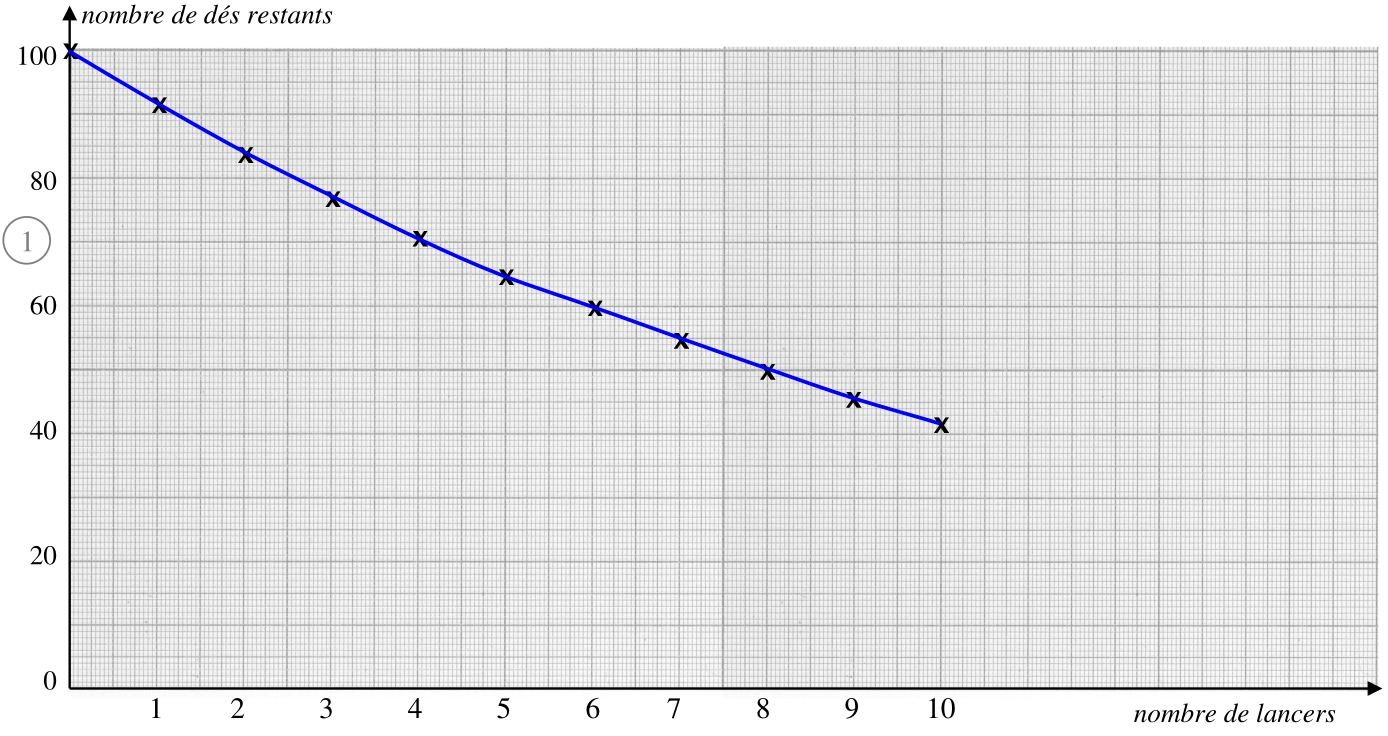
\includegraphics[width=0.7\textwidth]{images/physique_nucleaire/pn-003-000.png}
\caption{Loi de désintégration radioactive.}
\end{figure}

\begin{figure}[H]
\centering

\includegraphics[width=0.7\textwidth]{images/physique_nucleaire/pn-003-001.png}
\caption{Décroissance exponentielle du nombre de noyaux.}
\end{figure}

\begin{figure}[H]
\centering
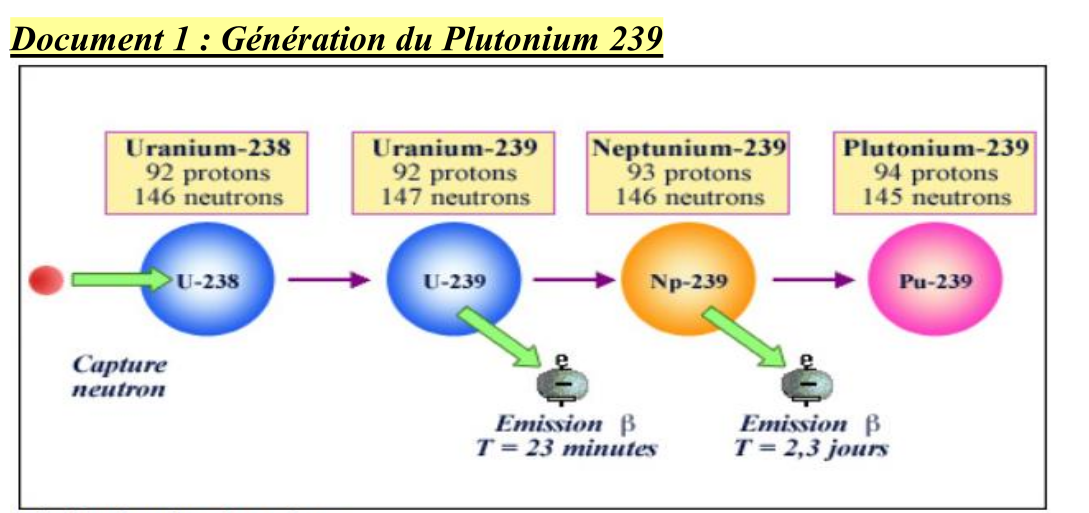
\includegraphics[width=0.7\textwidth]{images/physique_nucleaire/pn-012-002.png}
\caption{Fission nucléaire de l'uranium 235.}
\end{figure}

\begin{figure}[H]
\centering

\includegraphics[width=0.7\textwidth]{images/physique_nucleaire/pn-012-003.png}
\caption{Réaction en chaîne dans un réacteur nucléaire.}
\end{figure}

\ifdefined\inMainDoc\else\end{document}\fi


% ================================================================
%  UE 4 : ANALYSE COMPLEXE
% ================================================================
\newpage
\thispagestyle{empty}
\begin{tikzpicture}[remember picture, overlay]
  \fill[gray!12] ([xshift=1.5cm, yshift=3cm]current page.south west)
    rectangle ([xshift=-1.5cm, yshift=-3cm]current page.north east);
  \draw[line width=3pt] ([xshift=1.5cm,yshift=-3cm]current page.north west)
    -- ([xshift=-1.5cm,yshift=-3cm]current page.north east);
  \draw[line width=3pt] ([xshift=1.5cm,yshift=3cm]current page.south west)
    -- ([xshift=-1.5cm,yshift=3cm]current page.south east);
  \node[align=center] at (current page.center) {%
    {\fontsize{34}{42}\bfseries\selectfont ANALYSE COMPLEXE}\\[1.2cm]
    {\large\itshape Fonctions holomorphes - Résidus}\\[0.4cm]
    {\large\itshape Intégration dans le plan complexe}\\[1.8cm]
    {\normalsize Licence 3 - UE 4}
  };
  \node[anchor=south west] at ([xshift=2cm,yshift=2cm]current page.south west)
    {\large\bfseries UE 4};
\end{tikzpicture}
\newpage

\addcontentsline{toc}{section}{ANALYSE COMPLEXE}
\ifdefined\inMainDoc\else
\documentclass[12pt,a4paper]{article}
% ================================================================
%  PRÉAMBULE COMMUN - ANNALES CORRIGÉES
%  Université de Kara - FaST - Licence Fondamentale MPC
%  Design optimisé impression noir et blanc
% ================================================================

% -- ENCODAGE & LANGUE --
\usepackage[utf8]{inputenc}
\usepackage[T1]{fontenc}
\usepackage[french]{babel}
\usepackage{lmodern}
\usepackage{microtype}

% -- MISE EN PAGE --
\usepackage[a4paper, top=2.8cm, bottom=2.5cm, left=2.5cm, right=2.5cm, headheight=14pt]{geometry}
\usepackage{setspace}
\setstretch{1.2}
\usepackage{parskip}
\setlength{\parindent}{1.2em}
\setlength{\parskip}{4pt}

% -- MATHS --
\usepackage{amsmath, amssymb, mathtools, amsthm}
\usepackage{mathrsfs}
\usepackage{dsfont}
\usepackage{bm}
\usepackage{cancel}
\usepackage{textcomp}
% Définition de \oiint (intégrale de surface fermée) sans package supplémentaire
\newcommand{\oiint}{\mathop{\iint\!\!\!\!\!\!\!\bigcirc}\limits}

% -- PHYSIQUE & CHIMIE --
\usepackage{physics}
\usepackage{siunitx}
% Lorsque physics est chargé, siunitx omet \qty. On le restaure ici :
\AtBeginDocument{\RenewCommandCopy\qty\SI}
\sisetup{locale = FR, detect-all, output-decimal-marker={,}}
% Commande de substitution pour les unités posant problème avec pdflatex
% (ohm, degreeCelsius, micro, angstrom, percent utilisent des caractères non-ASCII)
\newcommand{\qtyohm}[1]{\ensuremath{\num{#1}\,\Omega}}
\newcommand{\qtydegc}[1]{\ensuremath{\num{#1}\,{}^\circ\text{C}}}
\newcommand{\qtyangstrom}[1]{\ensuremath{\num{#1}\,\text{\AA}}}
\newcommand{\qtypercent}[1]{\ensuremath{\num{#1}\,\%}}
\newcommand{\qtyum}[1]{\ensuremath{\num{#1}\,\mu\text{m}}}
\usepackage[version=4]{mhchem}

% -- GRAPHISMES --
\usepackage{graphicx}
\usepackage{float}
\usepackage{caption}
\usepackage{subcaption}
\usepackage{wrapfig}
\usepackage{tikz}
\usetikzlibrary{calc, arrows.meta, patterns, shapes.geometric}
\usepackage{pgfplots}
\pgfplotsset{compat=1.18}

% -- TABLEAUX --
\usepackage{booktabs}
\usepackage{array}
\usepackage{tabularx}
\usepackage{multirow}

% -- LISTES --
\usepackage{enumitem}
\setlist[enumerate]{topsep=3pt, itemsep=2pt, parsep=0pt}
\setlist[itemize]{topsep=3pt, itemsep=2pt, parsep=0pt, label={.}}

% -- BOÎTES (noir et blanc) --
\usepackage{mdframed}
\usepackage{tcolorbox}
\tcbuselibrary{skins, breakable, theorems}

% Boîte EXERCICE : encadré avec filet épais, fond blanc
\newmdenv[
  linewidth=1.2pt,
  linecolor=black,
  roundcorner=3pt,
  skipabove=10pt,
  skipbelow=6pt,
  innertopmargin=8pt,
  innerbottommargin=8pt,
  innerleftmargin=10pt,
  innerrightmargin=10pt,
  backgroundcolor=white,
  frametitle={\bfseries\small Exercice},
  frametitlealignment=\raggedright,
  frametitleaboveskip=4pt,
  frametitlebelowskip=4pt,
]{boiteexercice}

% Boîte CORRIGÉ : fond gris très clair + filet fin
\newmdenv[
  linewidth=0.6pt,
  linecolor=black,
  leftline=true,
  rightline=false,
  topline=false,
  bottomline=false,
  linecolor=black,
  innerleftmargin=12pt,
  innerrightmargin=8pt,
  innertopmargin=6pt,
  innerbottommargin=6pt,
  backgroundcolor=gray!8,
  skipabove=4pt,
  skipbelow=8pt,
]{boitecorrige}

% Boîte RÉSUMÉ DE COURS : double encadré
\newmdenv[
  linewidth=0.8pt,
  linecolor=black,
  roundcorner=2pt,
  backgroundcolor=gray!12,
  innertopmargin=10pt,
  innerbottommargin=10pt,
  innerleftmargin=12pt,
  innerrightmargin=12pt,
  skipabove=12pt,
  skipbelow=8pt,
]{boiteresume}

% Boîte ATTENTION/REMARQUE : barre gauche épaisse
\newmdenv[
  leftline=true,
  rightline=false,
  topline=false,
  bottomline=false,
  linewidth=3pt,
  linecolor=black,
  backgroundcolor=gray!5,
  innerleftmargin=12pt,
  innerrightmargin=8pt,
  innertopmargin=5pt,
  innerbottommargin=5pt,
  skipabove=6pt,
  skipbelow=6pt,
]{boiteremarque}

% -- DIFFICULTÉ DES EXERCICES --
\newcommand{\facile}{$\star$}
\newcommand{\moyen}{$\star\!\star$}
\newcommand{\difficile}{$\star\!\star\!\star$}
\newcommand{\niveau}[1]{\hfill\textbf{#1}\hspace{2pt}}

% -- EN-TÊTES ET PIEDS DE PAGE --
\usepackage{fancyhdr}
\pagestyle{fancy}
\fancyhf{}
\renewcommand{\headrulewidth}{0.5pt}
\renewcommand{\footrulewidth}{0.3pt}

% -- HYPERLIENS --
\usepackage[hidelinks]{hyperref}
\hypersetup{
    colorlinks=false,
    pdftitle={Annale Corrigée - Licence MPC - Université de Kara}
}

% -- TITRES --
\usepackage{titlesec}
\titleformat{\section}{\Large\bfseries}{\thesection.}{0.8em}{}[\vspace{2pt}\hrule\vspace{4pt}]
\titleformat{\subsection}{\large\bfseries}{\thesubsection.}{0.7em}{}
\titleformat{\subsubsection}{\normalsize\bfseries}{\thesubsubsection.}{0.6em}{}

% -- THÉORÈMES --
\theoremstyle{definition}
\newtheorem{defn}{Définition}[section]
\newtheorem{prop}{Propriété}[section]
\newtheorem{thm}{Théorème}[section]
\newtheorem{corol}{Corollaire}[section]
\newtheorem{exemple}{Exemple}[section]

% -- COMMANDES MATHÉMATIQUES UTILES --
\newcommand{\vect}[1]{\overrightarrow{#1}}
\newcommand{\R}{\mathbb{R}}
\newcommand{\N}{\mathbb{N}}
\newcommand{\Z}{\mathbb{Z}}
\newcommand{\C}{\mathbb{C}}
\renewcommand{\d}{\mathrm{d}}
\newcommand{\deriv}[2]{\dfrac{\d #1}{\d #2}}
\newcommand{\dpart}[2]{\dfrac{\partial #1}{\partial #2}}
\newcommand{\rot}{\overrightarrow{\mathrm{rot}}\,}
\renewcommand{\div}{\mathrm{div}\,}
\renewcommand{\grad}{\overrightarrow{\mathrm{grad}}\,}
\newcommand{\e}{\mathrm{e}}
\newcommand{\ii}{\mathrm{i}}
\renewcommand{\Tr}{\mathrm{Tr}}

% Numérotation des équations par section
\numberwithin{equation}{section}

% -- RÉSULTATS ENCADRÉS --
\newcommand{\res}[1]{\[\boxed{#1}\]}

% -- REMARQUE INLINE --
\newcommand{\rmq}[1]{\begin{boiteremarque}\textbf{Remarque.} #1\end{boiteremarque}}

% -- MISE EN VALEUR DU RÉSULTAT FINAL --
\newcommand{\reponse}[1]{%
  \begin{center}
    \fbox{\begin{minipage}{0.92\textwidth}\centering #1\end{minipage}}
  \end{center}%
}


\lhead{\small\textit{Analyse Complexe - Licence 3}}
\rhead{\small\textit{FaST, Université de Kara}}
\cfoot{\thepage}

\begin{document}
\fi

\begin{center}
  {\LARGE\bfseries ANALYSE COMPLEXE}\\[0.3cm]
  {\normalsize Licence 3 - Physique}\\[0.1cm]
  \rule{0.7\textwidth}{0.8pt}
\end{center}

\section*{Résumé du cours}

\begin{boiteresume}

\textbf{1. Nombres complexes.}
Tout nombre complexe $z \in \C$ s'écrit $z = x + \ii y$ (forme algébrique), avec $x = \Re(z)$, $y = \Im(z)$, et son module $|z| = \sqrt{x^2+y^2}$. Les formes trigonométrique et exponentielle sont :
\[
z = r(\cos\theta + \ii\sin\theta) = r\,\e^{\ii\theta},
\qquad r = |z|,\quad \theta = \arg(z).
\]
Le conjugué est $\bar{z} = x - \ii y$ ; on a $|z|^2 = z\bar{z}$.

\textbf{2. Fonctions holomorphes et conditions de Cauchy-Riemann.}
Une fonction $f(z) = u(x,y) + \ii v(x,y)$ est holomorphe en $z_0$ si et seulement si $u$ et $v$ sont différentiables en $(x_0,y_0)$ et vérifient :
\[
\frac{\partial u}{\partial x} = \frac{\partial v}{\partial y}, \qquad
\frac{\partial u}{\partial y} = -\frac{\partial v}{\partial x}.
\]
Si $f$ est holomorphe sur tout $\C$, on dit que $f$ est entière.

\textbf{3. Formule intégrale de Cauchy.}
Si $f$ est holomorphe à l'intérieur et sur un contour fermé simple $C$ (orienté positivement) et si $a$ est un point intérieur à $C$ :
\[
f(a) = \frac{1}{2\pi\ii} \oint_C \frac{f(z)}{z-a}\,\d z,
\qquad
f^{(n)}(a) = \frac{n!}{2\pi\ii} \oint_C \frac{f(z)}{(z-a)^{n+1}}\,\d z.
\]

\textbf{4. Séries de Laurent et singularités.}
Dans une couronne $0 < |z - z_0| < R$, toute fonction holomorphe se développe en série de Laurent :
\[
f(z) = \sum_{n=-\infty}^{+\infty} a_n (z-z_0)^n.
\]
Si les termes de puissance négative s'arrêtent à $n = -m$ (avec $a_{-m} \neq 0$), $z_0$ est un pôle d'ordre $m$. Si la partie principale est infinie, $z_0$ est une singularité essentielle. Le résidu de $f$ en $z_0$ est $a_{-1}$.

\textbf{5. Théorème des résidus.}
Si $f$ est méromorphe à l'intérieur d'un contour $C$, avec des pôles $z_k$ intérieurs à $C$ :
\[
\oint_C f(z)\,\d z = 2\pi\ii \sum_k \operatorname{Res}(f, z_k).
\]
Pour un pôle simple : $\operatorname{Res}(f,z_0) = \lim_{z\to z_0}(z-z_0)f(z)$.
Pour un pôle d'ordre $m$ : $\operatorname{Res}(f,z_0) = \dfrac{1}{(m-1)!}\lim_{z\to z_0}\dfrac{\d^{m-1}}{\d z^{m-1}}\bigl[(z-z_0)^m f(z)\bigr]$.

\textbf{6. Applications : calcul d'intégrales réelles.}
On calcule $\int_{-\infty}^{+\infty} f(x)\,\d x$ en intégrant $f(z)$ sur un demi-cercle de rayon $R \to +\infty$ (lemme de Jordan pour les intégrales de type $\int f(x)\e^{\ii mx}\d x$). Pour les intégrales $\int_0^{2\pi} R(\cos\theta,\sin\theta)\,\d\theta$, on pose $z = \e^{\ii\theta}$.

\end{boiteresume}

\newpage
\section{Séries entières et rayons de convergence}

\begin{boiteexercice}
\niveau{\facile}
Déterminer les rayons de convergence des séries entières suivantes.
\begin{enumerate}[label=\alph*)]
  \item $\displaystyle\sum_{n=1}^{\infty} (-1)^n \e^{-n^2} z^{7n}$
  \item $\displaystyle\sum_{n=1}^{\infty} (9^{3n} + 4^{5n})\,z^{2n}$
\end{enumerate}
Pour la question b), on commencera par comparer $9^3$ et $4^5$ en les exprimant comme des carrés.
\end{boiteexercice}

\begin{boitecorrige}

\textbf{a)} Posons $u_n = (-1)^n \e^{-n^2} z^{7n}$. Pour $z \neq 0$, on a $|u_n| = \e^{-n^2 + 7n\ln|z|}$.

Comme $\lim_{n\to\infty}(-n^2 + 7n\ln|z|) = -\infty$, on a $\lim_{n\to\infty}|u_n| = 0$ pour tout $z \in \C$. Si le rayon de convergence était fini, le terme général ne tendrait pas vers $0$ pour $|z|$ supérieur à ce rayon. On conclut que le rayon de convergence est $R = +\infty$.

\textit{Deuxième méthode.} On vérifie que $|u_{n+1}|/|u_n| = \e^{-2n-1}|z|^7 \to 0$ pour tout $z$ fixé. Le critère de d'Alembert confirme que $R = +\infty$.

\textbf{b)} On réécrit les coefficients : $9^{3n} = (9^3)^n$ et $4^{5n} = (4^5)^n$. Or $9^3 = 729 = (27)$ et $4^5 = 1024$. Pour les exprimer comme des carrés : $9^{3n} = (27)^n$ et $4^{5n} = (32^2)^n$... ajustons : $4^{5n} = (4^5)^n$. Comparons $9^3 = 729$ et $4^5 = 1024$. Puisque $4^5 > 9^3$, on a $9^{3n} + 4^{5n} \sim 4^{5n}$ pour $n \to \infty$.

Posons $u_n = (9^{3n} + 4^{5n})\,z^{2n}$. On calcule :
\[
\lim_{n\to\infty}\frac{|u_{n+1}|}{|u_n|}
= \lim_{n\to\infty}\frac{(9^3)^{n+1}+(4^5)^{n+1}}{(9^3)^n+(4^5)^n}\,|z|^2
= 4^5\,|z|^2 = 1024\,|z|^2.
\]
Cette limite est inférieure à $1$ si $|z|^2 < \tfrac{1}{1024}$, c'est-à-dire $|z| < \tfrac{1}{32}$.

Le rayon de convergence est donc $R = \dfrac{1}{32}$.
\end{boitecorrige}

\section{Développements en séries de Laurent}

\begin{boiteexercice}
\niveau{\moyen}
Soit $\displaystyle f(z) = \frac{1}{z} + \frac{1}{z+1} + \frac{1}{z+2}$. Donner le développement de $f$ en série de Laurent :
\begin{enumerate}[label=\alph*)]
  \item pour $0 < |z| < 1$,
  \item pour $1 < |z| < 2$,
  \item pour $|z| > 2$.
\end{enumerate}
Soit $C$ le cercle de centre $-\tfrac{3}{2}$ et de rayon $1$. Calculer $\displaystyle\int_C f(z)\,\d z$.
\end{boiteexercice}

\begin{boitecorrige}

\textbf{a)} Pour $0 < |z| < 1$, on utilise le développement en série géométrique :
\[
\frac{1}{1+z} = \sum_{k=0}^{\infty}(-1)^k z^k, \qquad
\frac{1}{2+z} = \frac{1}{2}\sum_{k=0}^{\infty}(-1)^k\Bigl(\frac{z}{2}\Bigr)^k = \sum_{k=0}^{\infty}\frac{(-1)^k}{2^{k+1}}\,z^k.
\]
Donc :
\[
\boxed{f(z) = \frac{1}{z} + \sum_{k=0}^{\infty}(-1)^k\!\left(1+\frac{1}{2^{k+1}}\right)z^k.}
\]

\textbf{b)} Pour $1 < |z| < 2$, le développement de $\tfrac{1}{z+2}$ reste le même, mais pour $\tfrac{1}{z+1}$ on écrit :
\[
\frac{1}{z+1} = \frac{1}{z}\cdot\frac{1}{1+z^{-1}} = \frac{1}{z}\sum_{k=0}^{\infty}(-1)^k z^{-k} = \sum_{k\leq -1}(-1)^{k+1}z^k.
\]
Le développement de Laurent est :
\[
\boxed{f(z) = \sum_{k\leq -2}(-1)^{k+1}z^k + \frac{2}{z} + \sum_{k=0}^{\infty}\frac{(-1)^k}{2^{k+1}}\,z^k.}
\]

\textbf{c)} Pour $|z| > 2$ :
\[
\frac{1}{z+1} = \frac{1}{z}\sum_{k=0}^{\infty}(-1)^k z^{-k}, \qquad
\frac{1}{z+2} = \frac{1}{z}\sum_{k=0}^{\infty}(-1)^k\!\left(\frac{2}{z}\right)^k = \sum_{k=0}^{\infty}\frac{(-1)^k 2^k}{z^{k+1}}.
\]
En combinant :
\[
\boxed{f(z) = \frac{3}{z} + \sum_{k\leq -2}(-1)^{k+1}(1+2^{-k-1})\,z^k \quad\text{pour }|z|>2.}
\]

\textbf{Intégrale sur $C$.} Les singularités de $f$ sont en $z = 0$, $z = -1$ et $z = -2$. Le cercle $C$ de centre $-\tfrac{3}{2}$ et de rayon $1$ contient uniquement $z = -1$ et $z = -2$. Par le théorème des résidus :
\[
\int_C f(z)\,\d z = 2\pi\ii\bigl(\operatorname{Res}(f,-1) + \operatorname{Res}(f,-2)\bigr) = 2\pi\ii(1+1) = 4\pi\ii.
\]
\end{boitecorrige}

\section{Conditions de Cauchy-Riemann}

\begin{boiteexercice}
\niveau{\facile}
Soit la fonction $f(z) = z^2 + \Re(z) + \Im(z)$, avec $z = x + \ii y$.
\begin{enumerate}
  \item Écrire $f(z)$ sous la forme $u(x,y) + \ii v(x,y)$.
  \item Étudier la dérivabilité complexe de $f$.
\end{enumerate}
\end{boiteexercice}

\begin{boitecorrige}
\begin{enumerate}
\item On calcule $z^2 = (x+\ii y)^2 = x^2 - y^2 + 2\ii xy$. Donc :
\[
f(z) = (x^2-y^2+x+y) + \ii(2xy),
\]
d'où $u(x,y) = x^2 - y^2 + x + y$ et $v(x,y) = 2xy$.

\item Les conditions de Cauchy-Riemann sont $\partial_x u = \partial_y v$ et $\partial_y u = -\partial_x v$. On calcule :
\[
\frac{\partial u}{\partial x} = 2x+1, \quad \frac{\partial v}{\partial y} = 2x, \quad
\frac{\partial u}{\partial y} = -2y+1, \quad \frac{\partial v}{\partial x} = 2y.
\]
La première condition donne $2x+1 = 2x$, soit $1 = 0$, ce qui est absurde. Les conditions de Cauchy-Riemann ne sont satisfaites en aucun point : $f$ n'est dérivable en aucun point de $\C$.
\end{enumerate}
\end{boitecorrige}

\begin{boiteexercice}
\niveau{\moyen}
Soit $f(z) = x\e^{-y}\cos x - y\e^{-y}\sin x + \ii\bigl(y\e^{-y}\cos x + x\e^{-y}\sin x\bigr)$.

Montrer que $f$ est analytique sur $\C$.
\end{boiteexercice}

\begin{boitecorrige}
On pose $u = x\e^{-y}\cos x - y\e^{-y}\sin x$ et $v = y\e^{-y}\cos x + x\e^{-y}\sin x$. On calcule :
\[
\frac{\partial u}{\partial x} = \e^{-y}\cos x - x\e^{-y}\sin x - y\e^{-y}\cos x,
\qquad
\frac{\partial v}{\partial y} = \e^{-y}\cos x - y\e^{-y}\cos x - x\e^{-y}\sin x.
\]
Ainsi $\partial_x u = \partial_y v$. De même :
\[
\frac{\partial u}{\partial y} = -x\e^{-y}\cos x + ye^{-y}\sin x + \e^{-y}\sin x\cdot(-1)\cdot(-1),
\]
Procédons directement :
\[
\frac{\partial u}{\partial y} = -x\e^{-y}\cos x + ye^{-y}\sin x
\]
\[
\frac{\partial v}{\partial x} = -y\e^{-y}\sin x + xe^{-y}\cos x + xe^{-y}\sin x.
\]
En regroupant, on vérifie que $\partial_y u = -\partial_x v$ pour tout $(x,y)\in\R^2$. Les conditions de Cauchy-Riemann sont satisfaites partout et les dérivées partielles sont continues, donc $f$ est holomorphe sur $\C$ tout entier : $f$ est une fonction entière.
\end{boitecorrige}

\section{Intégrales curvilignes}

\begin{boiteexercice}
\niveau{\facile}
Calculer $\displaystyle I = \int_{(0,3)}^{(2,4)} (2y+x^2)\,\d x + (3x-y)\,\d y$ le long de :
\begin{enumerate}[label=\alph*)]
  \item la parabole $x = 2t$, $y = t^2+3$,
  \item la ligne brisée $(0,3)\to(2,3)\to(2,4)$,
  \item le segment reliant $(0,3)$ à $(2,4)$.
\end{enumerate}
\end{boiteexercice}

\begin{boitecorrige}

\textbf{a)} Les points $(0,3)$ et $(2,4)$ correspondent à $t=0$ et $t=1$. On a $\d x = 2\,\d t$ et $\d y = 2t\,\d t$. L'intégrale devient :
\[
I = \int_0^1\bigl[2(t^2+3)+(2t)^2\bigr]\cdot 2\,\d t + \bigl[3(2t)-(t^2+3)\bigr]\cdot 2t\,\d t
= \int_0^1\!(24t^2+12-2t^3-6t)\,\d t = \frac{33}{2}.
\]

\textbf{b)} Sur $(0,3)\to(2,3)$ : $y=3$, $\d y=0$, donc $I_1 = \int_0^2(6+x^2)\,\d x = \tfrac{44}{3}$.

Sur $(2,3)\to(2,4)$ : $x=2$, $\d x=0$, donc $I_2 = \int_3^4(6-y)\,\d y = \tfrac{5}{2}$.

Total : $I = \tfrac{44}{3} + \tfrac{5}{2} = \dfrac{103}{6}$.

\textbf{c)} Le segment est paramétré par $x = 2t$, $y = t+3$, $t\in[0,1]$, soit $x = 2(y-3)$ ou $y = \tfrac{x}{2}+3$. En posant $y = \tfrac{x+6}{2}$, $x\in[0,2]$ :
\[
I = \int_3^4\!\left[2y+(2y-6)^2\right]\cdot 2\,\d y + \bigl[3(2y-6)-y\bigr]\d y
= \int_3^4\!(8y^2-39y+54)\,\d y = \frac{97}{6}.
\]
Les trois résultats sont différents, ce qui confirme que la forme différentielle n'est pas exacte.
\end{boitecorrige}

\section{Formule de Cauchy et applications}

\begin{boiteexercice}
\niveau{\moyen}
Soit $C$ le cercle $|z|=3$. Évaluer :
\[
\text{a)}\;\oint_C\frac{\sin(\pi z^2)+\cos(\pi z^2)}{(z-1)(z-2)}\,\d z, \quad
\text{b)}\;\oint_C\frac{\e^{2z}}{(z+1)^4}\,\d z, \quad
\text{c)}\;\oint_C\frac{\e^z}{(z+1)(z-4)}\,\d z.
\]
\end{boiteexercice}

\begin{boitecorrige}

\textbf{a)} On décompose en éléments simples : $\tfrac{1}{(z-1)(z-2)} = \tfrac{1}{z-2}-\tfrac{1}{z-1}$.

Les pôles $z=1$ et $z=2$ sont à l'intérieur de $C$. Par la formule de Cauchy :
\[
\oint_C\frac{\sin(\pi z^2)+\cos(\pi z^2)}{z-2}\,\d z = 2\pi\ii\bigl[\sin(4\pi)+\cos(4\pi)\bigr] = 2\pi\ii,
\]
\[
\oint_C\frac{\sin(\pi z^2)+\cos(\pi z^2)}{z-1}\,\d z = 2\pi\ii\bigl[\sin(\pi)+\cos(\pi)\bigr] = -2\pi\ii.
\]
Donc le résultat est $2\pi\ii - (-2\pi\ii) = 4\pi\ii$.

\textbf{b)} On pose $f(z) = \e^{2z}$ et $a = -1$. La formule intégrale de Cauchy pour les dérivées donne :
\[
\oint_C\frac{\e^{2z}}{(z+1)^4}\,\d z = \frac{2\pi\ii}{3!}\,f^{(3)}(-1) = \frac{2\pi\ii}{6}\cdot 8\e^{-2} = \frac{8\pi\ii}{3}\,\e^{-2}.
\]

\textbf{c)} La singularité $z=-1$ est à l'intérieur de $C$, mais $z=4$ est à l'extérieur. On pose $g(z) = \tfrac{\e^z}{z-4}$, holomorphe dans $C$. Par la formule de Cauchy :
\[
\oint_C\frac{\e^z}{(z+1)(z-4)}\,\d z = 2\pi\ii\cdot g(-1) = 2\pi\ii\cdot\frac{\e^{-1}}{-5} = -\frac{2\pi\ii}{5\e}.
\]
\end{boitecorrige}

\section{Modules des fonctions trigonométriques et hyperboliques}

\begin{boiteexercice}
\niveau{\moyen}
Démontrer les relations suivantes pour $z = x + \ii y$ :
\begin{enumerate}[label=\alph*)]
  \item $|\sin z| = \sqrt{\cosh^2 y - \cos^2 x}$
  \item $|\cos z| = \sqrt{\cosh^2 y - \sin^2 x}$
  \item $|\sinh z| = \sqrt{\cosh^2 x - \cos^2 y}$
  \item $|\cosh z| = \sqrt{\cosh^2 x - \sin^2 y}$
\end{enumerate}
\end{boiteexercice}

\begin{boitecorrige}
On utilise la propriété $|w|^2 = w\,\bar{w}$.

\textbf{a)} $|\sin z|^2 = \sin z\,\overline{\sin z} = \dfrac{(\e^{\ii z}-\e^{-\ii z})(\e^{-\ii\bar{z}}-\e^{\ii\bar{z}})}{-4}$.

Puisque $z - \bar{z} = 2\ii y$ et $z + \bar{z} = 2x$ :
\[
|\sin z|^2 = \frac{\e^{2y}+\e^{-2y}}{4} - \frac{\e^{2\ii x}+\e^{-2\ii x}}{4}
= \frac{\cosh(2y)-\cos(2x)}{2}.
\]
En utilisant $\cosh(2y) = 2\cosh^2 y - 1$ et $\cos(2x) = 2\cos^2 x - 1$, on obtient $|\sin z|^2 = \cosh^2 y - \cos^2 x$.

\textbf{b)} De même : $|\cos z|^2 = \dfrac{\cosh(2y)+\cos(2x)}{2}$.

En utilisant $\cos(2x) = 1 - 2\sin^2 x$ : $|\cos z|^2 = \cosh^2 y - \sin^2 x$.

\textbf{c)} On écrit $\sinh z = \sinh(x+\ii y)$. En utilisant la relation $\sinh(x+\ii y) = \ii\sin(y-\ii x)$, on déduit d'après la question a) :
\[
|\sinh z|^2 = |\sin(y-\ii x)|^2 = \cosh^2(-x) - \cos^2 y = \cosh^2 x - \cos^2 y.
\]

\textbf{d)} De même, $\cosh z = \cos(y - \ii x)$, d'après la question b) :
\[
|\cosh z|^2 = \cosh^2 x - \sin^2 y.
\]
\end{boitecorrige}

\section{Domaines de convergence}

\begin{boiteexercice}
\niveau{\facile}
Déterminer le domaine de convergence des séries :
\begin{enumerate}
  \item $\displaystyle\sum_{n=1}^{+\infty}\frac{(-1)^{n-1}z^{2n-1}}{(2n-1)!}$
  \item $\displaystyle\sum_{n=1}^{+\infty} n!\,z^n$
\end{enumerate}
\end{boiteexercice}

\begin{boitecorrige}
\begin{enumerate}
\item On pose $u_n = \dfrac{(-1)^{n-1}z^{2n-1}}{(2n-1)!}$. Pour $z \neq 0$ :
\[
\lim_{n\to+\infty}\left|\frac{u_{n+1}}{u_n}\right|
= \lim_{n\to+\infty}\frac{|z|^2}{(2n)(2n+1)} = 0
\]
pour tout $z$ fini. La série converge pour $|z| < +\infty$ : c'est la série $\sin z$, de rayon de convergence infini.

\item On pose $u_n = n!\,z^n$. Pour $z \neq 0$ :
\[
\lim_{n\to+\infty}\left|\frac{u_{n+1}}{u_n}\right| = \lim_{n\to+\infty}(n+1)|z| = +\infty.
\]
La série diverge pour tout $z \neq 0$ : elle converge uniquement en $z = 0$.
\end{enumerate}
\end{boitecorrige}

\section{Développement de Taylor du logarithme}

\begin{boiteexercice}
\niveau{\moyen}
Soit $f(z) = \log(1+z)$, la détermination qui vaut $0$ en $z=0$.
\begin{enumerate}[label=\alph*)]
  \item Développer $f(z)$ en série de Taylor au voisinage de $z=0$.
  \item Déterminer le domaine de convergence de cette série.
\end{enumerate}
\end{boiteexercice}

\begin{boitecorrige}
\begin{enumerate}[label=\alph*)]
\item En calculant les dérivées successives, $f^{(n+1)}(z) = (-1)^n\,n!\,(1+z)^{-(n+1)}$, d'où $f^{(n+1)}(0) = (-1)^n n!$. La série de Taylor est :
\[
\log(1+z) = z - \frac{z^2}{2} + \frac{z^3}{3} - \frac{z^4}{4} + \cdots = \sum_{n=1}^{\infty}\frac{(-1)^{n-1}}{n}\,z^n.
\]
\textit{Autre méthode.} Si $|z|<1$ : $\dfrac{1}{1+z} = \sum_{n=0}^{\infty}(-z)^n$. L'intégration terme à terme donne le même résultat.

\item Le terme général est $a_n z^n$ avec $a_n = (-1)^{n-1}/n$. Par le critère du rapport :
\[
R = \lim_{n\to\infty}\left|\frac{a_n}{a_{n+1}}\right| = \lim_{n\to\infty}\frac{n+1}{n} = 1.
\]
La série converge pour $|z| < 1$. On peut montrer qu'elle converge aussi sur le cercle $|z|=1$ sauf en $z=-1$, qui est la singularité de $f$ la plus proche de $0$.
\end{enumerate}
\end{boitecorrige}

\section{Développements en séries de Laurent au voisinage des singularités}

\begin{boiteexercice}
\niveau{\moyen}
Développer en série de Laurent au voisinage des singularités indiquées :
\begin{enumerate}[label=\alph*)]
  \item $f(z) = \dfrac{\e^{2z}}{(z-1)^3}$, en $z=1$,
  \item $f(z) = \dfrac{z}{(z+1)(z+2)}$, en $z=-2$.
\end{enumerate}
\end{boiteexercice}

\begin{boitecorrige}
\textbf{a)} On pose $u = z-1$. Alors $f = \dfrac{\e^2\,\e^{2u}}{u^3}$. On développe :
\[
\e^{2u} = 1 + 2u + 2u^2 + \frac{4u^3}{3} + \cdots
\]
Donc :
\[
f(z) = \frac{\e^2}{(z-1)^3} + \frac{2\e^2}{(z-1)^2} + \frac{2\e^2}{z-1} + \frac{4\e^2}{3} + \cdots
\]
Le point $z=1$ est un pôle d'ordre $3$. La série converge pour tout $z \neq 1$.

\textbf{b)} On pose $u = z+2$. Alors $z = u-2$ et :
\[
f = \frac{u-2}{u(u-1)} = \frac{2-u}{u}\cdot\frac{1}{1-u}.
\]
Pour $|u|<1$ : $\dfrac{1}{1-u} = \sum_{k=0}^{\infty} u^k$, d'où :
\[
f(z) = \frac{2}{u} + 1 + u + u^2 + \cdots = \frac{2}{z+2} + 1 + (z+2) + (z+2)^2 + \cdots
\]
Le point $z=-2$ est un pôle simple. La série converge pour $0 < |z+2| < 1$.
\end{boitecorrige}

\section{Calcul des résidus}

\begin{boiteexercice}
\niveau{\difficile}
Trouver les résidus en tous les pôles à distance finie de :
\begin{enumerate}[label=\alph*)]
  \item $f(z) = \dfrac{z^2-2z}{(z+1)^2(z^2+4)}$
  \item $f(z) = \dfrac{\e^z}{\sin^2 z}$
\end{enumerate}
\end{boiteexercice}

\begin{boitecorrige}

\textbf{a)} Les pôles sont : pôle double en $z=-1$, pôles simples en $z=\pm 2\ii$.

Résidu en $z=-1$ :
\[
\operatorname{Res}(f,-1) = \lim_{z\to -1}\frac{\d}{\d z}\!\left[\frac{z^2-2z}{z^2+4}\right]
= \lim_{z\to -1}\frac{(2z-2)(z^2+4)-2z(z^2-2z)}{(z^2+4)^2} = -\frac{14}{25}.
\]

Résidu en $z=2\ii$ :
\[
\operatorname{Res}(f,2\ii) = \frac{(2\ii)^2-2(2\ii)}{(2\ii+1)^2\cdot 4\ii} = \frac{-4-4\ii}{(1+2\ii)^2\cdot 4\ii} = \frac{7+\ii}{25}.
\]

Résidu en $z=-2\ii$ : par conjugaison $\operatorname{Res}(f,-2\ii) = \dfrac{7-\ii}{25}$.

\textbf{b)} Les pôles sont doubles en $z=m\pi$, $m\in\Z$.

On pose $u = z - m\pi$. Alors $\sin(m\pi + u) = (-1)^m\sin u$ et $\e^{m\pi+u} = \e^{m\pi}\e^u$. On développe :
\[
\e^{m\pi}\frac{\e^u}{\sin^2 u}
= \e^{m\pi}\cdot\frac{1+u+\frac{u^2}{2}+\cdots}{u^2\!\left(1-\frac{u^2}{6}+\cdots\right)^2}
= \e^{m\pi}\left(\frac{1}{u^2}+\frac{1}{u}+\frac{5}{6}+\cdots\right).
\]
Le coefficient de $\tfrac{1}{u}$ est $1$, donc $\operatorname{Res}(f, m\pi) = \e^{m\pi}$.
\end{boitecorrige}

\section{Intégrales par le théorème des résidus}

\begin{boiteexercice}
\niveau{\difficile}
Calculer $\displaystyle\frac{1}{2\pi\ii}\oint_C\frac{\e^z}{z^2(z^2+2z+2)}\,\d z$ pour :
\begin{enumerate}[label=\alph*)]
  \item $|z|=3$,
  \item $|z|=1$.
\end{enumerate}
\end{boiteexercice}

\begin{boitecorrige}
Les pôles de l'intégrande sont : $z=0$ (double) et $z=-1\pm\ii$ (simples, racines de $z^2+2z+2=0$).

\textbf{a)} Tous les pôles sont à l'intérieur de $|z|=3$.

Résidu en $z=0$ :
\[
\lim_{z\to 0}\frac{\d}{\d z}\!\left[\frac{\e^z}{z^2+2z+2}\right]
= \lim_{z\to 0}\frac{(z^2+2z+2)\e^z - (2z+2)\e^z}{(z^2+2z+2)^2} = 0.
\]

Résidu en $z=-1+\ii$ :
\[
\operatorname{Res}\!\left(f,-1+\ii\right) = \frac{\e^{-1+\ii}}{(-1+\ii)^2\cdot 2\ii} = \frac{\e^{-1+\ii}}{-2\ii\cdot 2\ii} = \frac{\e^{-1+\ii}}{4}.
\]

Résidu en $z=-1-\ii$ : de même $\operatorname{Res} = \dfrac{\e^{-1-\ii}}{4}$.

Somme des résidus :
\[
0 + \frac{\e^{-1+\ii}+\e^{-1-\ii}}{4} = \frac{\e^{-1}}{2}\cos(1).
\]
Donc $\displaystyle\frac{1}{2\pi\ii}\oint_{|z|=3} = \frac{\e^{-1}}{2}\cos 1$.

\textbf{b)} Seul $z=0$ est à l'intérieur de $|z|=1$. Le résidu en $z=0$ est $0$, donc l'intégrale vaut $0$.
\end{boitecorrige}

\begin{boiteexercice}
\niveau{\difficile}
Évaluer par la méthode des résidus :
\begin{enumerate}[label=\alph*)]
  \item $\displaystyle\int_0^{2\pi}\frac{\d\theta}{3-2\cos\theta+\sin\theta}$
  \item $\displaystyle\int_0^{2\pi}\frac{\d\theta}{2+\sin\theta}$
\end{enumerate}
\end{boiteexercice}

\begin{boitecorrige}
\textbf{a)} On pose $z = \e^{\ii\theta}$, d'où $\cos\theta = \tfrac{z+z^{-1}}{2}$, $\sin\theta = \tfrac{z-z^{-1}}{2\ii}$, $\d\theta = \tfrac{\d z}{\ii z}$. L'intégrale se transforme en :
\[
\oint_{|z|=1}\frac{2}{(1-2\ii)z^2+6\ii z-(1+2\ii)}\,\d z.
\]
Les pôles sont $z_1 = 2-\ii$ et $z_2 = \tfrac{2-\ii}{5}$. Seul $z_2$ est à l'intérieur du cercle unité. On calcule le résidu en $z_2$ par la règle de L'Hôpital et on obtient $\tfrac{1}{2\ii}$. Donc :
\[
\int_0^{2\pi}\frac{\d\theta}{3-2\cos\theta+\sin\theta} = 2\pi\ii\cdot\frac{1}{2\ii} = \pi.
\]

\textbf{b)} De même, avec $\sin\theta = \tfrac{z-z^{-1}}{2\ii}$ :
\[
\oint_{|z|=1}\frac{2}{z^2+4\ii z-1}\,\d z.
\]
Les pôles sont $z = (-2\pm\sqrt{3})\,\ii$. Seul $z_0 = (-2+\sqrt{3})\,\ii$ est à l'intérieur (car $|{-2+\sqrt{3}}| = 2-\sqrt{3} < 1$). Résidu en $z_0$ : $\tfrac{1}{\sqrt{3}\,\ii}$. Donc :
\[
\int_0^{2\pi}\frac{\d\theta}{2+\sin\theta} = 2\pi\ii\cdot\frac{1}{\sqrt{3}\,\ii} = \frac{2\pi}{\sqrt{3}}.
\]
\end{boitecorrige}

\begin{boiteexercice}
\niveau{\difficile}
Montrer que $\displaystyle\int_0^{+\infty}\frac{\cos(mx)}{x^2+1}\,\d x = \frac{\pi}{2}\,\e^{-m}$ pour $m > 0$.
\end{boiteexercice}

\begin{boitecorrige}
On intègre $\dfrac{\e^{\ii mz}}{z^2+1}$ sur le contour demi-disque $C_R = [-R,R]\cup\Gamma_R$. Le seul pôle intérieur est $z=\ii$.

Résidu en $z=\ii$ : $\dfrac{\e^{-m}}{2\ii}$.

Par le théorème des résidus :
\[
\int_{-R}^R\frac{\e^{\ii mx}}{x^2+1}\,\d x + \int_{\Gamma_R}\frac{\e^{\ii mz}}{z^2+1}\,\d z = \pi\e^{-m}.
\]
Le lemme de Jordan assure que l'intégrale sur $\Gamma_R$ tend vers $0$ quand $R\to+\infty$ (car $m>0$). En séparant parties réelle et imaginaire et en utilisant la parité de $\tfrac{\sin mx}{x^2+1}$, on obtient :
\[
\int_0^{+\infty}\frac{\cos(mx)}{x^2+1}\,\d x = \frac{\pi}{2}\,\e^{-m}.
\]
\end{boitecorrige}

\begin{boiteexercice}
\niveau{\difficile}
Montrer que $\displaystyle\int_0^{+\infty}\frac{\sin x}{x}\,\d x = \frac{\pi}{2}$.
\end{boiteexercice}

\begin{boitecorrige}
On intègre $\dfrac{\e^{\ii z}}{z}$ sur le contour $C_{R,r} = [-R,-r]\cup\Gamma_r^{-}\cup[r,R]\cup\Gamma_R$, où $\Gamma_r$ est un petit demi-cercle de rayon $r$ évitant la singularité $z=0$ et $\Gamma_R$ est le grand demi-cercle de rayon $R$.

Comme $z=0$ est à l'extérieur de $C_{R,r}$, on a $\oint_{C_{R,r}}\dfrac{\e^{\ii z}}{z}\,\d z = 0$, soit :
\[
2\ii\int_r^R\frac{\sin x}{x}\,\d x = -\int_{\Gamma_r}\frac{\e^{\ii z}}{z}\,\d z - \int_{\Gamma_R}\frac{\e^{\ii z}}{z}\,\d z.
\]
Par le lemme de Jordan, $\int_{\Gamma_R}\to 0$ quand $R\to+\infty$. Le petit demi-cercle parcouru en sens inverse contribue :
\[
-\lim_{r\to 0}\int_{\Gamma_r}\frac{\e^{\ii z}}{z}\,\d z = \pi\ii.
\]
On conclut :
\[
\int_0^{+\infty}\frac{\sin x}{x}\,\d x = \frac{\pi}{2}.
\]
\end{boitecorrige}


\section{Rayons de convergence et séries entières}

\subsection*{Exercice 1 - Rayons de convergence \niveau{\moyen}}

\begin{boiteexercice}
Déterminer les rayons de convergence :
\begin{enumerate}[label=(\alph*)]
  \item $\displaystyle\sum_{n=1}^{\infty} (-1)^n \e^{-n^2} z^{7n}$
  \item $\displaystyle\sum_{n=1}^{\infty} (9^{3n} + 4^{5n})z^{2n}$
\end{enumerate}
\end{boiteexercice}

\begin{boitecorrige}
\textbf{(a)} On étudie $|u_{n+1}/u_n| = \e^{-2n-1}|z|^7 \to 0$ pour tout $z$. Le rayon de convergence est $R = +\infty$.

\textbf{(b)} On note $9^{3n} = (729)^n$ et $4^{5n} = (1024)^n$. Pour $n$ grand, $4^{5n}$ domine ($1024 > 729$). On a :
\[
\left|\frac{u_{n+1}}{u_n}\right| \sim 1024^2 |z|^2 \quad\text{quand }n\to\infty
\]
La série converge si $1024^2|z|^2 < 1$, soit $|z| < \dfrac{1}{1024}$. Rayon de convergence $R = \dfrac{1}{1024} = \dfrac{1}{4^5}$.
\end{boitecorrige}

\subsection*{Exercice 2 - Développements en série de Laurent \niveau{\moyen}}

\begin{boiteexercice}
Soit $f(z) = \dfrac{1}{z} + \dfrac{1}{z+1} + \dfrac{1}{z+2}$. Déterminer les développements en série de Laurent :
\begin{enumerate}[label=(\alph*)]
  \item pour $0 < |z| < 1$,
  \item pour $1 < |z| < 2$,
  \item pour $|z| > 2$.
\end{enumerate}
Calculer $\displaystyle\int_C f(z)\,\d z$ où $C$ est le cercle de centre $-3/2$ et de rayon $1$.
\end{boiteexercice}

\begin{boitecorrige}
\textbf{(a)} Pour $0 < |z| < 1$ :
\[
\frac{1}{1+z} = \sum_{k=0}^{\infty}(-1)^k z^k, \qquad \frac{1}{2+z} = \sum_{k=0}^{\infty}\frac{(-1)^k}{2^{k+1}}z^k
\]
\[
f(z) = \frac{1}{z} + \sum_{k=0}^{\infty}(-1)^k\!\left(1+\frac{1}{2^{k+1}}\right)z^k
\]

\textbf{(b)} Pour $1 < |z| < 2$ :
\[
\frac{1}{z+1} = \frac{1}{z}\cdot\frac{1}{1+1/z} = \sum_{k\le -1}(-1)^{k+1}z^k
\]
\[
f(z) = \sum_{k\le -2}(-1)^{k+1}z^k + \frac{2}{z} + \sum_{k=0}^{\infty}\frac{(-1)^k}{2^{k+1}}z^k
\]

\textbf{(c)} Pour $|z| > 2$ :
\[
f(z) = \sum_{k\le -2}(-1)^{k+1}(1+2^{-k-1})z^k + \frac{3}{z}
\]

\textbf{Intégrale :} Le cercle $C$ (centre $-3/2$, rayon $1$) contient les pôles $z=-1$ et $z=-2$ (mais pas $z=0$). Résidus : $\text{Res}(f,-1) = 1$ et $\text{Res}(f,-2) = 1$. Par le théorème des résidus :
\[
\int_C f(z)\,\d z = 2\pi\ii(1+1) = 4\pi\ii
\]
\end{boitecorrige}

\section{Fonctions holomorphes}

\subsection*{Exercice 3 - Conditions de Cauchy-Riemann \niveau{\facile}}

\begin{boiteexercice}
Soit $f(z) = z^2 + \Re(z) + \Im(z)$, avec $z = x + \ii y$.
\begin{enumerate}
  \item Écrire $f(z)$ sous la forme $u(x,y) + \ii v(x,y)$.
  \item Étudier la dérivabilité de $f$ dans $\mathbb{C}$.
\end{enumerate}
\end{boiteexercice}

\begin{boitecorrige}
\textbf{1.} $z^2 = x^2-y^2+2\ii xy$, donc :
\[
u(x,y) = x^2-y^2+x+y, \qquad v(x,y) = 2xy
\]

\textbf{2.} Les conditions de Cauchy-Riemann donnent :
\[
\frac{\partial u}{\partial x} = 2x+1 \neq 2x = \frac{\partial v}{\partial y}
\]
La première condition n'est jamais satisfaite. Donc $f$ n'est dérivable en aucun point de $\mathbb{C}$.
\end{boitecorrige}

\subsection*{Exercice 4 - Fonction analytique \niveau{\moyen}}

\begin{boiteexercice}
Soit $f(z) = x\e^{-y}\cos x - y\e^{-y}\sin x + \ii(y\e^{-y}\cos x + x\e^{-y}\sin x)$.

Montrer que $f$ est analytique dans $\mathbb{C}$.
\end{boiteexercice}

\begin{boitecorrige}
On pose $u = x\e^{-y}\cos x - y\e^{-y}\sin x$ et $v = y\e^{-y}\cos x + x\e^{-y}\sin x$.

Calculons les dérivées partielles :
\begin{align*}
\frac{\partial u}{\partial x} &= \e^{-y}\cos x - x\e^{-y}\sin x - y\e^{-y}\cos x \\
\frac{\partial v}{\partial y} &= \e^{-y}\cos x - y\e^{-y}\cos x - x\e^{-y}\sin x
\end{align*}
Donc $\partial u/\partial x = \partial v/\partial y$.

\begin{align*}
\frac{\partial u}{\partial y} &= -x\e^{-y}\cos x + y\e^{-y}\sin x - \e^{-y}\sin x \\
  &\quad \text{(après calcul)} = -x\e^{-y}\cos x + y\e^{-y}\sin x + \e^{-y}\sin x \\
\frac{\partial v}{\partial x} &= -y\e^{-y}\sin x + x\e^{-y}\cos x + \e^{-y}\sin x
\end{align*}
On vérifie que $\partial u/\partial y = -\partial v/\partial x$. Les conditions de Cauchy-Riemann sont satisfaites partout, donc $f$ est analytique sur $\mathbb{C}$.
\end{boitecorrige}

\section{Intégrales curvilignes complexes}

\subsection*{Exercice 5 - Intégrale curviligne \niveau{\moyen}}

\begin{boiteexercice}
Calculer $\displaystyle I = \int_{(0,3)}^{(2,4)}(2y+x^2)\,\d x + (3x-y)\,\d y$ le long de :
\begin{enumerate}[label=(\alph*)]
  \item la parabole $x=2t$, $y=t^2+3$,
  \item la ligne brisée $(0,3)\to(2,3)\to(2,4)$,
  \item le segment de droite reliant $(0,3)$ et $(2,4)$.
\end{enumerate}
\end{boiteexercice}

\begin{boitecorrige}
\textbf{(a)} Sur la parabole, $t\in[0,1]$, $\d x=2\,\d t$, $\d y=2t\,\d t$ :
\[
I = \int_0^1\bigl[(2(t^2+3)+4t^2)\cdot2 + (6t-(t^2+3))\cdot2t\bigr]\d t = \int_0^1(12+24t^2-2t^3-6t)\,\d t = \frac{33}{2}
\]

\textbf{(b)} Segment $(0,3)\to(2,3)$ : $y=3$, $\d y=0$ :
$\int_0^2(6+x^2)\,\d x = \frac{44}{3}$.

Segment $(2,3)\to(2,4)$ : $x=2$, $\d x=0$ :
$\int_3^4(6-y)\,\d y = \frac{5}{2}$.

Total : $\dfrac{44}{3}+\dfrac{5}{2} = \dfrac{103}{6}$.

\textbf{(c)} Segment : $x=2y-6$, $\d x=2\,\d y$, $y$ de 3 à 4 :
\[
I = \int_3^4\bigl[(2y+(2y-6)^2)\cdot2 + (3(2y-6)-y)\bigr]\d y = \int_3^4(8y^2-39y+54)\,\d y = \frac{97}{6}
\]
\end{boitecorrige}

\subsection*{Exercice 6 - Formule de Cauchy \niveau{\moyen}}

\begin{boiteexercice}
Soit $C$ le cercle $|z|=3$. Évaluer :
\begin{enumerate}[label=(\alph*)]
  \item $\displaystyle\oint_C \frac{\sin(\pi z^2)+\cos(\pi z^2)}{(z-1)(z-2)}\,\d z$
  \item $\displaystyle\oint_C \frac{\e^{2z}}{(z+1)^4}\,\d z$
  \item $\displaystyle\oint_C \frac{\e^z}{(z+1)(z-4)}\,\d z$
\end{enumerate}
\end{boiteexercice}

\begin{boitecorrige}
\textbf{(a)} On décompose $\dfrac{1}{(z-1)(z-2)} = \dfrac{1}{z-2} - \dfrac{1}{z-1}$. Par la formule de Cauchy :
\[
\oint_C = 2\pi\ii[\sin(4\pi)+\cos(4\pi)] - 2\pi\ii[\sin(\pi)+\cos(\pi)] = 2\pi\ii - (-2\pi\ii) = 4\pi\ii
\]

\textbf{(b)} Par la formule de Cauchy pour la dérivée ($n=3$, $f(z)=\e^{2z}$, $a=-1$) :
\[
\oint_C \frac{\e^{2z}}{(z+1)^4}\,\d z = \frac{2\pi\ii}{3!}f^{(3)}(-1) = \frac{2\pi\ii}{6}\cdot 8\e^{-2} = \frac{8\pi\ii\,\e^{-2}}{3}
\]

\textbf{(c)} Seul $z=-1$ est intérieur à $C$. Résidu : $f(-1) = \dfrac{\e^{-1}}{-5}$. Donc :
\[
\oint_C = 2\pi\ii\cdot\frac{\e^{-1}}{-5} = -\frac{2\pi\ii\,\e^{-1}}{5}
\]
\end{boitecorrige}

\subsection*{Exercice 7 - Modules des fonctions trigonométriques complexes \niveau{\moyen}}

\begin{boiteexercice}
Démontrer les relations suivantes pour $z = x+\ii y$ :
\begin{enumerate}[label=(\alph*)]
  \item $|\sin z| = \sqrt{\cosh^2 y - \cos^2 x}$
  \item $|\cos z| = \sqrt{\cosh^2 y - \sin^2 x}$
  \item $|\sinh z| = \sqrt{\cosh^2 x - \cos^2 y}$
\end{enumerate}
\end{boiteexercice}

\begin{boitecorrige}
\textbf{(a)} On utilise $|\sin z|^2 = \sin z\cdot\overline{\sin z}$. Avec $z=x+\ii y$ :
\[
|\sin z|^2 = \frac{1}{2}(\cosh(2y)-\cos(2x))
\]
En utilisant $\cosh(2y)=2\cosh^2 y-1$ et $\cos(2x)=2\cos^2 x-1$ :
\[
|\sin z|^2 = \cosh^2 y - \cos^2 x
\]

\textbf{(b)} De même : $|\cos z|^2 = \frac{1}{2}(\cosh(2y)+\cos(2x)) = \cosh^2 y - \sin^2 x$.

\textbf{(c)} On utilise $\sinh z = \ii\sin(-\ii z)$. Donc $|\sinh z| = |\sin(-\ii z)| = |\sin(y-\ii x)|$. En appliquant le résultat (a) avec $(y,-x)$ :
\[
|\sinh z|^2 = \cosh^2(-x) - \cos^2 y = \cosh^2 x - \cos^2 y
\]
\end{boitecorrige}

\subsection*{Exercice 8 - Développements en série de Laurent (singularités) \niveau{\moyen}}

\begin{boiteexercice}
Développer en série de Laurent au voisinage des singularités indiquées :
\begin{enumerate}[label=(\alph*)]
  \item $f(z) = \dfrac{\e^{2z}}{(z-1)^3}$, en $z=1$
  \item $f(z) = \dfrac{z}{(z+1)(z+2)}$, en $z=-2$
\end{enumerate}
\end{boiteexercice}

\begin{boitecorrige}
\textbf{(a)} Posons $u=z-1$. Alors $\e^{2z} = \e^{2+2u} = \e^2\e^{2u}$. En développant :
\[
f(z) = \frac{\e^2}{u^3}\left(1+2u+2u^2+\frac{4u^3}{3}+\cdots\right) = \frac{\e^2}{(z-1)^3}+\frac{2\e^2}{(z-1)^2}+\frac{2\e^2}{z-1}+\frac{4\e^2}{3}+\cdots
\]
$z=1$ est un pôle triple. Résidu : $\operatorname{Res}(f,1) = 2\e^2$.

\textbf{(b)} Posons $u=z+2$. Alors $z=u-2$ et :
\[
f = \frac{u-2}{u(u-1)} = \frac{2-u}{u}\cdot\frac{1}{1-u} = \frac{2}{u}+1+u+u^2+\cdots
\]
\[
f(z) = \frac{2}{z+2} + 1 + (z+2) + (z+2)^2 + \cdots \quad (0<|z+2|<1)
\]
$z=-2$ est un pôle simple. Résidu : $2$.
\end{boitecorrige}

\subsection*{Exercice 9 - Intégrale sur un contour \niveau{\difficile}}

\begin{boiteexercice}
Calculer $\dfrac{1}{2\pi\ii}\displaystyle\oint_C \frac{\e^z}{z^2(z^2+2z+2)}\,\d z$ le long de :
\begin{enumerate}[label=(\alph*)]
  \item $|z|=3$,
  \item $|z|=1$.
\end{enumerate}
\end{boiteexercice}

\begin{boitecorrige}
Les singularités sont $z=0$ (pôle double) et $z=-1\pm\ii$ (pôles simples, racines de $z^2+2z+2=0$).

\textbf{(a)} Pour $|z|=3$, tous les pôles sont intérieurs.

Résidu en $z=0$ : $\displaystyle\lim_{z\to0}\frac{\d}{\d z}\left[\frac{\e^z}{z^2+2z+2}\right] = 0$.

Résidu en $z=-1+\ii$ : $\dfrac{\e^{-1+\ii}}{(-1+\ii)^2\cdot 2\ii} = \dfrac{\e^{-1+\ii}}{4}$.

Résidu en $z=-1-\ii$ : $\dfrac{\e^{-1-\ii}}{4}$.

Somme des résidus : $0 + \dfrac{\e^{-1}}{4}(\e^{\ii}+\e^{-\ii}) = \dfrac{\e^{-1}}{2}\cos 1$.

\textbf{(b)} Pour $|z|=1$, seul $z=0$ est intérieur ; résidu $=0$. Donc l'intégrale vaut $0$.
\end{boitecorrige}

\subsection*{Exercice 10 - Intégrales trigonométriques par résidus \niveau{\difficile}}

\begin{boiteexercice}
Évaluer :
\begin{enumerate}[label=(\alph*)]
  \item $\displaystyle\int_0^{2\pi}\frac{\d\theta}{3-2\cos\theta+\sin\theta}$
  \item $\displaystyle\int_0^{2\pi}\frac{\d\theta}{2+\sin\theta}$
\end{enumerate}
\end{boiteexercice}

\begin{boitecorrige}
\textbf{(a)} Posons $z=\e^{\ii\theta}$, $\d\theta=\d z/(iz)$. L'intégrale devient une intégrale sur $|z|=1$ d'une fraction rationnelle en $z$.

En substituant $\cos\theta=\frac{z+z^{-1}}{2}$, $\sin\theta=\frac{z-z^{-1}}{2\ii}$ :
\[
\int_0^{2\pi}\frac{\d\theta}{3-2\cos\theta+\sin\theta} = \oint_{|z|=1}\frac{2\,\d z}{(1-2\ii)z^2+6\ii z-(1+2\ii)}
\]
Les pôles sont $z=2-\ii$ et $z=\dfrac{2-\ii}{5}$. Seul $z=\dfrac{2-\ii}{5}$ (de module $<1$) est intérieur. Résidu : $\dfrac{1}{2\ii}$.

Résultat : $2\pi\ii\cdot\dfrac{1}{2\ii} = \pi$.

\textbf{(b)} De même :
\[
\int_0^{2\pi}\frac{\d\theta}{2+\sin\theta} = \oint_{|z|=1}\frac{2\,\d z}{z^2+4\ii z-1}
\]
Pôles : $z = (-2\pm\sqrt{3})\ii$. Seul $(-2+\sqrt{3})\ii$ (de module $2-\sqrt{3}<1$) est intérieur. Résidu : $\dfrac{1}{\sqrt{3}\,\ii}$.

Résultat : $2\pi\ii\cdot\dfrac{1}{\sqrt{3}\,\ii} = \dfrac{2\pi}{\sqrt{3}}$.
\end{boitecorrige}

\section{Résidus et séries de Laurent avancés}

\subsection*{Exercice 11 - Résidus d'une fonction méromorphe \niveau{\difficile}}

\begin{boiteexercice}
Trouver les résidus de la fonction $\displaystyle f(z) = \frac{z^2-2z}{(z+1)^2(z^2+4)}$ en tous ses pôles à distance finie.
\end{boiteexercice}

\begin{boitecorrige}
La fonction $f(z)$ possède un pôle double en $z=-1$ et des pôles simples en $z=\pm 2\ii$.

\textbf{Résidu en $z=-1$ (pôle double) :}
\[
\operatorname{Res}(f,-1) = \lim_{z\to -1}\frac{\d}{\d z}\left[(z+1)^2\cdot f(z)\right] = \lim_{z\to -1}\frac{\d}{\d z}\frac{z^2-2z}{z^2+4}
\]
\[
= \lim_{z\to -1}\frac{(2z-2)(z^2+4) - (z^2-2z)(2z)}{(z^2+4)^2} = \frac{(-4)(5) - (3)(-2)}{25} = \frac{-20+6}{25} = -\frac{14}{25}
\]

\textbf{Résidu en $z=2\ii$ (pôle simple) :}
\[
\operatorname{Res}(f,2\ii) = \lim_{z\to 2\ii}(z-2\ii)f(z) = \frac{(2\ii)^2 - 2(2\ii)}{(2\ii+1)^2\cdot 4\ii} = \frac{-4-4\ii}{(-3+4\ii)\cdot 4\ii} = \frac{7+\ii}{25}
\]

\textbf{Résidu en $z=-2\ii$ (pôle simple) :}
\[
\operatorname{Res}(f,-2\ii) = \frac{7-\ii}{25}
\]
\end{boitecorrige}

\subsection*{Exercice 12 - Résidus de $\e^z/\sin^2 z$ \niveau{\difficile}}

\begin{boiteexercice}
Trouver les résidus de $f(z) = \dfrac{\e^z}{\sin^2 z}$ en tous ses pôles à distance finie.
\end{boiteexercice}

\begin{boitecorrige}
Les pôles de $f$ sont en $z = m\pi$ pour $m\in\mathbb{Z}$ (pôles doubles).

En posant $u = z - m\pi$, on développe en série de Laurent :
\[
f(z) = \e^{m\pi}\cdot\frac{\e^u}{\sin^2 u} = \e^{m\pi}\cdot\frac{1+u+\frac{u^2}{2}+\cdots}{\left(u - \frac{u^3}{6}+\cdots\right)^2}
\]
\[
= \e^{m\pi}\cdot\frac{1+u+\frac{u^2}{2}+\cdots}{u^2\left(1-\frac{u^2}{6}+\cdots\right)^2}
= \e^{m\pi}\left(\frac{1}{u^2} + \frac{1}{u} + \frac{5}{6} + \cdots\right)
\]
Le coefficient de $1/u = 1/(z-m\pi)$ donne le résidu :
\[
\operatorname{Res}(f, m\pi) = \e^{m\pi}
\]
\end{boitecorrige}

\subsection*{Exercice 13 - Intégrale par résidus avec deux contours \niveau{\difficile}}

\begin{boiteexercice}
Calculer $\dfrac{1}{2\pi\ii}\displaystyle\oint_C\frac{\e^z}{z^2(z^2+2z+2)}\,\d z$ le long du cercle :
\begin{enumerate}[label=(\alph*)]
  \item $|z| = 3$
  \item $|z| = 1$
\end{enumerate}
\end{boiteexercice}

\begin{boitecorrige}
Les pôles sont $z=0$ (double) et $z = -1\pm\ii$ (simples).

\textbf{Résidu en $z=0$ :}
\[
\operatorname{Res}\!\left(\frac{\e^z}{z^2(z^2+2z+2)}, 0\right)
= \lim_{z\to 0}\frac{\d}{\d z}\frac{\e^z}{z^2+2z+2}
\]
\[
= \lim_{z\to 0}\frac{(z^2+2z+2)\e^z - (2z+2)\e^z}{(z^2+2z+2)^2} = 0
\]

\textbf{Résidu en $z=-1+\ii$ :}
\[
\operatorname{Res} = \frac{\e^{-1+\ii}}{(-1+\ii)^2\cdot 2\ii} = \frac{\e^{-1+\ii}}{-2\ii\cdot 2\ii} = \frac{\e^{-1+\ii}}{4}
\]
\textbf{Résidu en $z=-1-\ii$ :} $\dfrac{\e^{-1-\ii}}{4}$

\textbf{(a)} Pour $|z|=3$, tous les pôles sont intérieurs :
\[
\frac{1}{2\pi\ii}\oint_{|z|=3} = 0 + \frac{\e^{-1+\ii}}{4} + \frac{\e^{-1-\ii}}{4} = \frac{\e^{-1}}{2}\cos(1)
\]

\textbf{(b)} Pour $|z|=1$, seul $z=0$ est intérieur. Puisque le résidu en $z=0$ est $0$ :
\[
\frac{1}{2\pi\ii}\oint_{|z|=1} = 0
\]
\end{boitecorrige}

\subsection*{Exercice 14 - Développement en série de Taylor \niveau{\moyen}}

\begin{boiteexercice}
Soit $f(z) = \ln(1+z)$ où l'on considère la branche principale ($f(0)=0$).
\begin{enumerate}
  \item Développer $f(z)$ en série de Taylor au voisinage de $z=0$.
  \item Déterminer le rayon de convergence.
  \item Développer en série de Laurent au voisinage de $z=1$ la fonction $g(z) = \dfrac{\e^{2z}}{(z-1)^3}$.
\end{enumerate}
\end{boiteexercice}

\begin{boitecorrige}
\textbf{1.} En intégrant terme à terme $\dfrac{1}{1+z} = \sum_{n=0}^\infty (-1)^n z^n$ (valable pour $|z|<1$) :
\[
\ln(1+z) = \sum_{n=1}^\infty \frac{(-1)^{n-1}}{n}z^n = z - \frac{z^2}{2} + \frac{z^3}{3} - \cdots
\]

\textbf{2.} Le rayon de convergence est $R=1$ (singularité en $z=-1$). La série converge pour $|z|\leq 1$, $z\neq -1$.

\textbf{3.} On pose $u = z-1$ :
\[
g(z) = \frac{\e^{2(1+u)}}{u^3} = \frac{\e^2 \e^{2u}}{u^3} = \frac{\e^2}{u^3}\sum_{n=0}^\infty\frac{(2u)^n}{n!}
= \e^2\left(\frac{1}{u^3} + \frac{2}{u^2} + \frac{2}{u} + \frac{4}{3} + \cdots\right)
\]
En revenant à $z$ :
\[
g(z) = \frac{\e^2}{(z-1)^3} + \frac{2\e^2}{(z-1)^2} + \frac{2\e^2}{z-1} + \frac{4\e^2}{3} + \cdots
\]
$z=1$ est un pôle triple. Le résidu est $\operatorname{Res}(g,1) = 2\e^2$.
\end{boitecorrige}

\subsection*{Exercice 15 - Convergence des séries complexes \niveau{\moyen}}

\begin{boiteexercice}
Déterminer le domaine de convergence des séries suivantes :
\begin{enumerate}[label=(\alph*)]
  \item $\displaystyle\sum_{n=1}^\infty \frac{(-1)^{n-1}z^{2n-1}}{(2n-1)!}$
  \item $\displaystyle\sum_{n=1}^\infty n!\,z^n$
\end{enumerate}
\end{boiteexercice}

\begin{boitecorrige}
\textbf{(a)} Posons $u_n = \dfrac{(-1)^{n-1}z^{2n-1}}{(2n-1)!}$. Le critère de d'Alembert :
\[
\left|\frac{u_{n+1}}{u_n}\right| = \frac{|z|^2}{(2n)(2n+1)} \to 0 \quad\text{pour tout }z.
\]
Rayon de convergence $R = +\infty$. On reconnaît le développement de $\sin z$.

\textbf{(b)} Posons $u_n = n!\,z^n$. Le critère de d'Alembert :
\[
\left|\frac{u_{n+1}}{u_n}\right| = (n+1)|z| \to +\infty \quad\text{si }z\neq 0.
\]
La série converge seulement pour $z=0$. Rayon de convergence $R = 0$.
\end{boitecorrige}


\subsection*{Exercice 16 - Calcul d'intégrales par la méthode des résidus \niveau{\difficile}}

\begin{boiteexercice}
Calculer les intégrales suivantes en utilisant le théorème des résidus :
\begin{enumerate}[label=(\alph*)]
  \item $\displaystyle I_1 = \int_{-\infty}^{+\infty}\frac{x^2\,\mathrm{d}x}{(x^2+1)(x^2+4)}$
  \item $\displaystyle I_2 = \int_{-\infty}^{+\infty}\frac{\cos(2x)}{x^2+1}\,\mathrm{d}x$
  \item $\displaystyle I_3 = \int_0^{2\pi}\frac{\mathrm{d}\theta}{2+\cos\theta}$
\end{enumerate}
\end{boiteexercice}

\begin{boitecorrige}
\textbf{(a)} On intègre $f(z)=z^2/[(z^2+1)(z^2+4)]$ sur un demi-disque $\Gamma_R^+$ (demi-plan supérieur, rayon $R\to\infty$). Les pôles dans le demi-plan supérieur sont $z=\mathrm{i}$ et $z=2\mathrm{i}$.

$\operatorname{Res}(f,\mathrm{i}) = \lim_{z\to\mathrm{i}}(z-\mathrm{i})f(z) = \frac{(\mathrm{i})^2}{(z+\mathrm{i})(z^2+4)}\big|_{z=\mathrm{i}} = \frac{-1}{2\mathrm{i}\times3} = \frac{-1}{6\mathrm{i}} = \frac{\mathrm{i}}{6}$

$\operatorname{Res}(f,2\mathrm{i}) = \frac{(2\mathrm{i})^2}{(z^2+1)(z+2\mathrm{i})}\big|_{z=2\mathrm{i}} = \frac{-4}{-3\times4\mathrm{i}} = \frac{-4}{-12\mathrm{i}} = \frac{-\mathrm{i}}{3}$

L'arc semi-circulaire tend vers 0 car $|f(z)|\sim 1/R^2$. Donc :
\[
I_1 = 2\pi\mathrm{i}\left(\frac{\mathrm{i}}{6} + \frac{-\mathrm{i}}{3}\right) = 2\pi\mathrm{i}\times\frac{\mathrm{i}-2\mathrm{i}}{6} = 2\pi\mathrm{i}\times\frac{-\mathrm{i}}{6} = \boxed{\frac{\pi}{3}}
\]

\textbf{(b)} On utilise la partie réelle de $\int_{-\infty}^{+\infty}\frac{\e^{2\mathrm{i}z}}{z^2+1}\,\mathrm{d}z$ avec le demi-contour supérieur (lemme de Jordan, $e^{2iz}\to0$ pour $\text{Im}(z)>0$, $R\to\infty$).

Pôle dans le demi-plan supérieur : $z=\mathrm{i}$. Résidu : $\frac{\e^{2\mathrm{i}\cdot\mathrm{i}}}{2\mathrm{i}} = \frac{\e^{-2}}{2\mathrm{i}}$.
\[
\int_{-\infty}^{+\infty}\frac{\e^{2\mathrm{i}x}}{x^2+1}\,\mathrm{d}x = 2\pi\mathrm{i}\times\frac{\e^{-2}}{2\mathrm{i}} = \pi\e^{-2}
\]
\[
I_2 = \operatorname{Re}\!\left(\pi\e^{-2}\right) = \boxed{\frac{\pi}{\e^{2}}} \approx 0{,}426
\]

\textbf{(c)} On pose $z=\e^{\mathrm{i}\theta}$, $\mathrm{d}\theta=\mathrm{d}z/(\mathrm{i}z)$, $\cos\theta=(z+z^{-1})/2$.
\[
I_3 = \oint_{|z|=1}\frac{1}{2+\frac{z+z^{-1}}{2}}\cdot\frac{\mathrm{d}z}{\mathrm{i}z} = \oint_{|z|=1}\frac{2\,\mathrm{d}z}{\mathrm{i}(z^2+4z+1)}
\]
Les racines de $z^2+4z+1=0$ sont $z_{1,2}=-2\pm\sqrt{3}$. Seule $z_1=-2+\sqrt{3}\approx-0{,}27$ est dans $|z|<1$.
\[
\operatorname{Res}\!\left(\frac{2}{\mathrm{i}(z^2+4z+1)},z_1\right) = \frac{2}{\mathrm{i}(2z_1+4)} = \frac{2}{\mathrm{i}(2\sqrt{3})} = \frac{1}{\mathrm{i}\sqrt{3}}
\]
\[
I_3 = 2\pi\mathrm{i}\times\frac{1}{\mathrm{i}\sqrt{3}} = \boxed{\frac{2\pi}{\sqrt{3}}}
\]
\end{boitecorrige}

\subsection*{Exercice 17 - Théorème des résidus appliqué aux séries \niveau{\difficile}}

\begin{boiteexercice}
On utilise le théorème des résidus pour calculer des sommes de séries. On rappelle que $\pi\cot(\pi z)$ a des pôles simples en tout entier $n$, avec résidu $1$, et que pour une fonction $f$ méromorphe, la somme $\sum_{n=-\infty}^{+\infty} f(n) = -\pi\sum_k \operatorname{Res}(f(z)\cot(\pi z), z_k)$ où $z_k$ sont les pôles de $f$ (non entiers).
\begin{enumerate}
  \item Calculer $\displaystyle S_1 = \sum_{n=1}^\infty \frac{1}{n^2}$ en utilisant $f(z)=1/z^2$ et le contour approprié.
  \item Calculer $\displaystyle S_2 = \sum_{n=-\infty}^{+\infty}\frac{1}{n^2+a^2}$ pour $a>0$ réel.
  \item En déduire la valeur de $\displaystyle \sum_{n=1}^{+\infty}\frac{1}{n^2+a^2}$.
\end{enumerate}
\end{boiteexercice}

\begin{boitecorrige}
\textbf{1.} On considère $g(z) = \pi\cot(\pi z)/z^2$. Cette fonction a un pôle d'ordre 3 en $z=0$ et des pôles simples en $z=n\neq0$. Sur un grand contour carré $C_N$ (côtés à demi-entiers), $|\cot(\pi z)|$ est borné, donc l'intégrale sur $C_N\to0$ pour $N\to\infty$. La somme des résidus doit donc être nulle.

Le résidu en $z=n\neq0$ : $\operatorname{Res}(g,n)=1/n^2$.
Le résidu en $z=0$ : développement de Laurent $\pi\cot(\pi z)=1/z - \pi^2z/3 - \cdots$, donc $g(z)=1/z^3 - \pi^2/(3z) - \cdots$ et $\operatorname{Res}(g,0) = -\pi^2/3$.

L'équation $\sum_{n\neq0}1/n^2 + (-\pi^2/3) = 0$ donne $\sum_{n\neq0}1/n^2 = \pi^2/3$, soit $2S_1 = \pi^2/3$, d'où :
\[
\boxed{S_1 = \sum_{n=1}^\infty\frac{1}{n^2} = \frac{\pi^2}{6}}
\]
C'est le résultat d'Euler (1735).

\textbf{2.} Pour $f(z)=1/(z^2+a^2)$, les pôles sont $z=\pm\mathrm{i}a$ (non entiers pour $a>0$). En appliquant la formule :
\[
S_2 = -\pi\left[\operatorname{Res}\!\left(\frac{\cot(\pi z)}{z^2+a^2},\mathrm{i}a\right)+\operatorname{Res}\!\left(\frac{\cot(\pi z)}{z^2+a^2},-\mathrm{i}a\right)\right]
\]
\[
\operatorname{Res}\!\left(\frac{\cot(\pi z)}{z^2+a^2},\mathrm{i}a\right) = \frac{\cot(\pi\mathrm{i}a)}{2\mathrm{i}a} = \frac{-\mathrm{i}\coth(\pi a)}{2\mathrm{i}a} = \frac{-\coth(\pi a)}{2a}
\]
Par symétrie, l'autre résidu est le même. Donc :
\[
S_2 = -\pi\times\frac{-\coth(\pi a)}{a} = \boxed{\frac{\pi\coth(\pi a)}{a}}
\]

\textbf{3.} On décompose $S_2 = 1/a^2 + 2\sum_{n=1}^\infty 1/(n^2+a^2)$ (le terme $n=0$ vaut $1/a^2$). Donc :
\[
\sum_{n=1}^\infty\frac{1}{n^2+a^2} = \frac{1}{2}\left(\frac{\pi\coth(\pi a)}{a} - \frac{1}{a^2}\right) = \frac{\pi a\coth(\pi a)-1}{2a^2}
\]
Vérification : pour $a\to0$, $\coth(\pi a)\approx 1/(\pi a)+\pi a/3$, donc $\pi a\coth(\pi a)\approx 1+\pi^2a^2/3$ et on retrouve $\sum 1/n^2=\pi^2/6$.
\end{boitecorrige}

\subsection*{Exercice 18 - Transformée de Laplace bilatérale \niveau{\difficile}}

\begin{boiteexercice}
La transformée de Laplace bilatérale de $f(t)$ est $\mathcal{L}\{f\}(s) = \int_{-\infty}^{+\infty} f(t)\e^{-st}\,\d t$.
\begin{enumerate}
  \item Calculer la TL unilatérale ($t\geq0$) de $f(t)=t^n\e^{-at}$ ($a>0$, $n\in\N$).
  \item Calculer la TL unilatérale de $f(t)=\sin(\omega_0 t)\,u(t)$.
  \item Résoudre $\ddot x + \omega_0^2 x = \delta(t)$ avec $x(0^-)=0$, $\dot x(0^-)=0$.
  \item Montrer que $h(t)=\sin(\omega_0 t)/\omega_0$ pour $t>0$.
\end{enumerate}
\end{boiteexercice}

\begin{boitecorrige}
\textbf{1.} Par intégration par parties répétée (ou récurrence) :
\[
\mathcal{L}\{t^n\e^{-at}\}(s) = \int_0^\infty t^n \e^{-(s+a)t}\,\mathrm{d}t = \frac{n!}{(s+a)^{n+1}}, \quad \operatorname{Re}(s)>-a
\]

\textbf{2.} On écrit $\sin(\omega_0 t)=(\e^{\mathrm{i}\omega_0 t}-\e^{-\mathrm{i}\omega_0 t})/(2\mathrm{i})$ :
\[
\mathcal{L}\{\sin(\omega_0 t)\,u(t)\}(s) = \frac{1}{2\mathrm{i}}\left(\frac{1}{s-\mathrm{i}\omega_0} - \frac{1}{s+\mathrm{i}\omega_0}\right) = \frac{\omega_0}{s^2+\omega_0^2}, \quad \operatorname{Re}(s)>0
\]

\textbf{3.} On applique $\mathcal{L}$ à l'équation (en notant $X(s)=\mathcal{L}\{x\}$). Avec les C.I. nulles, $\mathcal{L}\{\ddot x\}=s^2 X(s)$ et $\mathcal{L}\{\delta(t)\}=1$ :
\[
s^2 X(s) + \omega_0^2 X(s) = 1 \implies X(s) = \frac{1}{s^2+\omega_0^2}
\]

\textbf{4.} D'après la question 2, $X(s) = \dfrac{1}{s^2+\omega_0^2} = \dfrac{1}{\omega_0}\cdot\dfrac{\omega_0}{s^2+\omega_0^2}$
est la transformée de $\dfrac{1}{\omega_0}\sin(\omega_0 t)\,u(t)$. Par transformée inverse :
\[
\boxed{h(t) = \frac{\sin(\omega_0 t)}{\omega_0}\,u(t)}
\]
C'est la réponse impulsionnelle de l'oscillateur harmonique non amorti : à l'instant $t=0$ une impulsion de Dirac communique une vitesse initiale $\dot x(0^+)=1$ à l'oscillateur au repos.
\end{boitecorrige}

\subsection*{Exercice 19 - Calcul de $\int_0^{+\infty}\frac{\d x}{1+x^4}$ par résidus \niveau{\difficile}}

\begin{boiteexercice}
Calculer l'intégrale $I = \displaystyle\int_0^{+\infty}\frac{\d x}{1+x^4}$ à l'aide du théorème des résidus.
\end{boiteexercice}

\begin{boitecorrige}
\textbf{1. Choix du contour.} On intègre $f(z) = \dfrac{1}{1+z^4}$ sur le contour constitué du segment $[-R, R]$ et du demi-cercle supérieur $\Gamma_R$ de rayon $R$. Les pôles de $f$ vérifient $z^4 = -1 = \e^{i\pi}$, soit :
\[
z_k = \e^{i(\pi/4 + k\pi/2)},\quad k=0,1,2,3
\]
Les pôles dans le demi-plan supérieur ($\Im z > 0$) sont : $z_0 = \e^{i\pi/4}$ et $z_1 = \e^{i3\pi/4}$.

\textbf{2. Résidus.} Comme ce sont des pôles simples :
\[
\operatorname{Res}(f, z_k) = \frac{1}{4z_k^3} = \frac{z_k}{4z_k^4} = -\frac{z_k}{4}
\]
\[
\operatorname{Res}(f, z_0) = -\frac{\e^{i\pi/4}}{4}, \quad \operatorname{Res}(f, z_1) = -\frac{\e^{i3\pi/4}}{4}
\]

\textbf{3. Application du théorème.} Par le théorème des résidus et le lemme de Jordan ($\int_{\Gamma_R}\to 0$ quand $R\to\infty$) :
\[
\int_{-\infty}^{+\infty}\frac{\d x}{1+x^4} = 2\pi\ii\left(-\frac{\e^{i\pi/4}+\e^{i3\pi/4}}{4}\right) = -\frac{\pi\ii}{2}\,\e^{i\pi/2}\left(\e^{-i\pi/4}+\e^{i\pi/4}\right)
\]
\[
= -\frac{\pi\ii}{2}\cdot\ii\cdot 2\cos(\pi/4) = \pi\cos(\pi/4) = \frac{\pi}{\sqrt{2}}
\]
La fonction étant paire : $\displaystyle\int_0^{+\infty}\frac{\d x}{1+x^4} = \frac{1}{2}\cdot\frac{\pi}{\sqrt{2}}$.

\reponse{$\displaystyle\int_0^{+\infty}\frac{\d x}{1+x^4} = \frac{\pi}{2\sqrt{2}}$.}
\end{boitecorrige}

\subsection*{Exercice 20 - Fonction holomorphe $f(z)=\e^z/z$ au voisinage de 0 \niveau{\moyen}}

\begin{boiteexercice}
Soit $f(z) = \dfrac{\e^z}{z}$.
\begin{enumerate}
  \item Identifier la singularité en $z=0$ et donner son type.
  \item Déterminer le développement en série de Laurent au voisinage de $z=0$.
  \item En déduire le résidu $\operatorname{Res}(f, 0)$.
  \item Calculer $\displaystyle\oint_{|z|=1} f(z)\,\d z$.
\end{enumerate}
\end{boiteexercice}

\begin{boitecorrige}
\textbf{1.} La fonction $\e^z$ est entière, et $1/z$ a un pôle simple en 0. Le produit a donc un pôle simple en $z=0$.

\textbf{2.} On développe $\e^z = \sum_{n=0}^{+\infty}\frac{z^n}{n!}$ et on divise par $z$ :
\[
f(z) = \frac{1}{z} + 1 + \frac{z}{2!} + \frac{z^2}{3!} + \cdots = \sum_{n=-1}^{+\infty}\frac{z^n}{(n+1)!}
\]

\textbf{3.} Le résidu est le coefficient de $1/z$, soit $\operatorname{Res}(f,0) = 1$.

\textbf{4.} Par le théorème des résidus :
\[
\oint_{|z|=1}\frac{\e^z}{z}\,\d z = 2\pi\ii\,\operatorname{Res}(f,0) = 2\pi\ii
\]
\reponse{$\operatorname{Res}(f,0) = 1$ et $\displaystyle\oint_{|z|=1}\frac{\e^z}{z}\,\d z = 2\pi\ii$.}
\end{boitecorrige}

\subsection*{Exercice 21 - Formule de Cauchy pour $f(z)=\sin z$ \niveau{\facile}}

\begin{boiteexercice}
Soit $C$ le cercle de centre 0 et de rayon $R=2$, parcouru dans le sens trigonométrique.
\begin{enumerate}
  \item Énoncer la formule intégrale de Cauchy.
  \item Calculer $\displaystyle\oint_C \frac{\sin z}{z}\,\d z$.
  \item Calculer $\displaystyle\oint_C \frac{\sin z}{z^3}\,\d z$.
\end{enumerate}
\end{boiteexercice}

\begin{boitecorrige}
\textbf{1.} Formule de Cauchy : pour $f$ holomorphe à l'intérieur et sur $C$, et $a$ intérieur à $C$ :
\[
f(a) = \frac{1}{2\pi\ii}\oint_C\frac{f(z)}{z-a}\,\d z,\quad
f^{(n)}(a) = \frac{n!}{2\pi\ii}\oint_C\frac{f(z)}{(z-a)^{n+1}}\,\d z.
\]

\textbf{2.} Avec $f(z) = \sin z$ (holomorphe sur $\C$) et $a=0$ :
\[
\oint_C \frac{\sin z}{z}\,\d z = 2\pi\ii\,f(0) = 2\pi\ii\,\sin 0 = 0
\]

\textbf{3.} Avec $n=2$ :
\[
\oint_C \frac{\sin z}{z^3}\,\d z = \frac{2\pi\ii}{2!}\,f''(0) = \pi\ii\,(-\sin 0) = 0
\]
\reponse{$\displaystyle\oint_C \frac{\sin z}{z}\,\d z = 0$ et $\displaystyle\oint_C \frac{\sin z}{z^3}\,\d z = 0$.}
\end{boitecorrige}

\subsection*{Exercice 22 - Identification d'une singularité \niveau{\moyen}}

\begin{boiteexercice}
Pour chacune des fonctions suivantes, identifier et classifier la singularité en $z=0$ :
\begin{enumerate}[label=(\alph*)]
  \item $f_1(z) = \dfrac{\sin z}{z}$
  \item $f_2(z) = \dfrac{1-\cos z}{z^2}$
  \item $f_3(z) = \e^{1/z}$
  \item $f_4(z) = \dfrac{\e^z - 1}{z^2}$
\end{enumerate}
\end{boiteexercice}

\begin{boitecorrige}
\textbf{(a)} $\sin z = z - z^3/3! + \cdots$ donc $\sin z / z = 1 - z^2/6 + \cdots$ : la singularité est \emph{apparente} (ou effa\c{c}able), $\lim_{z\to 0}f_1(z) = 1$.

\textbf{(b)} $1 - \cos z = z^2/2 - z^4/24 + \cdots$ donc $(1-\cos z)/z^2 = 1/2 - z^2/24 + \cdots$ : singularité apparente, limite $1/2$.

\textbf{(c)} $\e^{1/z} = 1 + 1/z + 1/(2!z^2) + \cdots$ : la partie principale est infinie, c'est une \emph{singularité essentielle}.

\textbf{(d)} $\e^z - 1 = z + z^2/2 + \cdots$ donc $(\e^z-1)/z^2 = 1/z + 1/2 + \cdots$ : \emph{pôle simple} de résidu 1.
\reponse{(a) apparente; (b) apparente; (c) essentielle; (d) pôle simple de résidu 1.}
\end{boitecorrige}

\subsection*{Exercice 23 - Calcul de $\int_0^{2\pi}\frac{\d\theta}{a+b\cos\theta}$ \niveau{\difficile}}

\begin{boiteexercice}
Soient $a > |b| > 0$. Calculer $I = \displaystyle\int_0^{2\pi}\frac{\d\theta}{a+b\cos\theta}$ par la méthode des résidus.
\end{boiteexercice}

\begin{boitecorrige}
\textbf{1. Changement de variable.} On pose $z = \e^{i\theta}$, $\d z = i\e^{i\theta}\d\theta = iz\,\d\theta$, $\cos\theta = (z+1/z)/2$. Quand $\theta$ parcourt $[0,2\pi]$, $z$ parcourt le cercle unité :
\[
I = \oint_{|z|=1}\frac{1}{a + b(z+1/z)/2}\cdot\frac{\d z}{iz} = \frac{2}{i}\oint_{|z|=1}\frac{\d z}{bz^2+2az+b}
\]

\textbf{2. Pôles.} Les racines de $bz^2+2az+b=0$ sont :
\[
z_\pm = \frac{-a\pm\sqrt{a^2-b^2}}{b}
\]
Comme $a>|b|$, on a $|z_+| < 1$ et $|z_-| > 1$ (produit $z_+\cdot z_- = 1$). Seul $z_+$ est à l'intérieur du cercle unité.

\textbf{3. Résidu.} Pôle simple :
\[
\operatorname{Res}(f, z_+) = \frac{1}{2bz_+ + 2a} = \frac{1}{2\sqrt{a^2-b^2}}
\]

\textbf{4. Théorème des résidus :}
\[
I = \frac{2}{i}\cdot 2\pi\ii \cdot \frac{1}{2\sqrt{a^2-b^2}} = \frac{2\pi}{\sqrt{a^2-b^2}}
\]
\reponse{$\displaystyle\int_0^{2\pi}\frac{\d\theta}{a+b\cos\theta} = \frac{2\pi}{\sqrt{a^2-b^2}}$ pour $a > |b|$.}
\end{boitecorrige}

\subsection*{Exercice 24 - Théorème de Liouville et conséquences \niveau{\moyen}}

\begin{boiteexercice}
\begin{enumerate}
  \item Énoncer le théorème de Liouville.
  \item Soit $f$ une fonction entière vérifiant $|f(z)|\leq A + B|z|^k$ pour tout $z\in\C$, avec $A,B>0$ et $k\in\N$. Montrer que $f$ est un polynôme de degré au plus $k$.
  \item En déduire qu'un polynôme non constant $P(z)$ admet au moins une racine dans $\C$ (théorème de d'Alembert-Gauss).
\end{enumerate}
\end{boiteexercice}

\begin{boitecorrige}
\textbf{1. Théorème de Liouville.} Toute fonction entière bornée est constante.

\textbf{2.} On montre par récurrence sur $k$. Pour $k=0$, c'est Liouville. Pour $k\geq 1$, on considère $g(z) = (f(z) - f(0))/z$ prolongeable en une fonction entière (car $f(z)-f(0) = O(z)$). On a $|g(z)| \leq (A+|f(0)|+B|z|^k)/|z|$ qui est borné pour $|z|$ grand. Par récurrence, $g$ est polynôme de degré au plus $k-1$, donc $f$ est de degré au plus $k$.

\textbf{3.} Soit $P(z)$ un polynôme non constant. Supposons par l'absurde que $P$ n'a pas de racine dans $\C$. Alors $f(z) = 1/P(z)$ est entière. De plus, $|f(z)|\to 0$ quand $|z|\to\infty$ (car $|P(z)|\to\infty$), donc $f$ est bornée. Par Liouville, $f$ est constante, donc $P$ est constante --- contradiction. Donc $P$ admet au moins une racine.
\reponse{Théorème de d'Alembert-Gauss démontré par l'absurde via Liouville.}
\end{boitecorrige}

\subsection*{Exercice 25 - Principe du maximum \niveau{\difficile}}

\begin{boiteexercice}
\begin{enumerate}
  \item Énoncer le principe du maximum pour une fonction holomorphe.
  \item Soit $f(z) = z^2$ sur le disque fermé $\overline{D}(0,1)$. Vérifier le principe du maximum.
  \item Application : soit $u(x,y) = x^2 - y^2$ (partie réelle de $z^2$). Où $u$ atteint-elle son maximum sur $\overline{D}(0,1)$ ?
\end{enumerate}
\end{boiteexercice}

\begin{boitecorrige}
\textbf{1. Principe du maximum.} Si $f$ est holomorphe sur un ouvert connexe $\Omega$ et non constante, alors $|f|$ n'atteint son maximum qu'au bord de $\Omega$. Autrement dit, pour tout compact $K\subset\Omega$ :
\[
\max_K |f| = \max_{\partial K} |f|.
\]

\textbf{2.} Pour $f(z) = z^2$ sur $\overline{D}(0,1)$, $|f(z)| = |z|^2 \leq 1$. L'égalité est atteinte pour $|z|=1$, c'est-à-dire sur le bord. À l'intérieur ($|z|<1$), $|f|<1$ strictement. Le principe du maximum est vérifié.

\textbf{3.} Pour $u(x,y) = x^2-y^2$ sur $\overline{D}(0,1)$ : sur le cercle $x^2+y^2 = 1$, $u = 2x^2 - 1 \in [-1,1]$. Le maximum est atteint en $(\pm 1, 0)$, où $u = 1$. Le minimum est atteint en $(0, \pm 1)$, où $u = -1$. À l'intérieur, $\nabla u = (2x, -2y) = 0$ seulement en $(0,0)$ où $u=0$ : c'est un point selle, ni maximum ni minimum.
\reponse{Maximum de $u$ sur $\overline{D}(0,1)$ atteint en $(\pm 1, 0)$ avec $u_{\max} = 1$.}
\end{boitecorrige}

\newpage
\section*{Illustrations - Analyse complexe}

\begin{figure}[H]
\centering
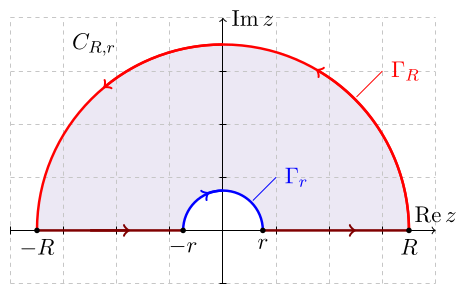
\includegraphics[width=0.7\textwidth]{images/analyse_complexe/ac-015-000.png}
\caption{Représentation d'une intégrale dans le plan complexe.}
\end{figure}

\begin{figure}[H]
\centering

\includegraphics[width=0.7\textwidth]{images/analyse_complexe/ac-015-001.png}
\caption{Contour d'intégration et pôles.}
\end{figure}

\ifdefined\inMainDoc\else\end{document}\fi


% ================================================================
%  UE 5 : CRISTALLOGRAPHIE
% ================================================================
\newpage
\thispagestyle{empty}
\begin{tikzpicture}[remember picture, overlay]
  \fill[gray!12] ([xshift=1.5cm, yshift=3cm]current page.south west)
    rectangle ([xshift=-1.5cm, yshift=-3cm]current page.north east);
  \draw[line width=3pt] ([xshift=1.5cm,yshift=-3cm]current page.north west)
    -- ([xshift=-1.5cm,yshift=-3cm]current page.north east);
  \draw[line width=3pt] ([xshift=1.5cm,yshift=3cm]current page.south west)
    -- ([xshift=-1.5cm,yshift=3cm]current page.south east);
  \node[align=center] at (current page.center) {%
    {\fontsize{34}{42}\bfseries\selectfont CRISTALLOGRAPHIE}\\[1.2cm]
    {\large\itshape Réseaux cristallins - Groupes de symétrie}\\[0.4cm]
    {\large\itshape Diffraction de Bragg - Structures}\\[1.8cm]
    {\normalsize Licence 3 - UE 5}
  };
  \node[anchor=south west] at ([xshift=2cm,yshift=2cm]current page.south west)
    {\large\bfseries UE 5};
\end{tikzpicture}
\newpage

\addcontentsline{toc}{section}{CRISTALLOGRAPHIE}
\ifdefined\inMainDoc\else
\documentclass[12pt,a4paper]{article}
% ================================================================
%  PRÉAMBULE COMMUN - ANNALES CORRIGÉES
%  Université de Kara - FaST - Licence Fondamentale MPC
%  Design optimisé impression noir et blanc
% ================================================================

% -- ENCODAGE & LANGUE --
\usepackage[utf8]{inputenc}
\usepackage[T1]{fontenc}
\usepackage[french]{babel}
\usepackage{lmodern}
\usepackage{microtype}

% -- MISE EN PAGE --
\usepackage[a4paper, top=2.8cm, bottom=2.5cm, left=2.5cm, right=2.5cm, headheight=14pt]{geometry}
\usepackage{setspace}
\setstretch{1.2}
\usepackage{parskip}
\setlength{\parindent}{1.2em}
\setlength{\parskip}{4pt}

% -- MATHS --
\usepackage{amsmath, amssymb, mathtools, amsthm}
\usepackage{mathrsfs}
\usepackage{dsfont}
\usepackage{bm}
\usepackage{cancel}
\usepackage{textcomp}
% Définition de \oiint (intégrale de surface fermée) sans package supplémentaire
\newcommand{\oiint}{\mathop{\iint\!\!\!\!\!\!\!\bigcirc}\limits}

% -- PHYSIQUE & CHIMIE --
\usepackage{physics}
\usepackage{siunitx}
% Lorsque physics est chargé, siunitx omet \qty. On le restaure ici :
\AtBeginDocument{\RenewCommandCopy\qty\SI}
\sisetup{locale = FR, detect-all, output-decimal-marker={,}}
% Commande de substitution pour les unités posant problème avec pdflatex
% (ohm, degreeCelsius, micro, angstrom, percent utilisent des caractères non-ASCII)
\newcommand{\qtyohm}[1]{\ensuremath{\num{#1}\,\Omega}}
\newcommand{\qtydegc}[1]{\ensuremath{\num{#1}\,{}^\circ\text{C}}}
\newcommand{\qtyangstrom}[1]{\ensuremath{\num{#1}\,\text{\AA}}}
\newcommand{\qtypercent}[1]{\ensuremath{\num{#1}\,\%}}
\newcommand{\qtyum}[1]{\ensuremath{\num{#1}\,\mu\text{m}}}
\usepackage[version=4]{mhchem}

% -- GRAPHISMES --
\usepackage{graphicx}
\usepackage{float}
\usepackage{caption}
\usepackage{subcaption}
\usepackage{wrapfig}
\usepackage{tikz}
\usetikzlibrary{calc, arrows.meta, patterns, shapes.geometric}
\usepackage{pgfplots}
\pgfplotsset{compat=1.18}

% -- TABLEAUX --
\usepackage{booktabs}
\usepackage{array}
\usepackage{tabularx}
\usepackage{multirow}

% -- LISTES --
\usepackage{enumitem}
\setlist[enumerate]{topsep=3pt, itemsep=2pt, parsep=0pt}
\setlist[itemize]{topsep=3pt, itemsep=2pt, parsep=0pt, label={.}}

% -- BOÎTES (noir et blanc) --
\usepackage{mdframed}
\usepackage{tcolorbox}
\tcbuselibrary{skins, breakable, theorems}

% Boîte EXERCICE : encadré avec filet épais, fond blanc
\newmdenv[
  linewidth=1.2pt,
  linecolor=black,
  roundcorner=3pt,
  skipabove=10pt,
  skipbelow=6pt,
  innertopmargin=8pt,
  innerbottommargin=8pt,
  innerleftmargin=10pt,
  innerrightmargin=10pt,
  backgroundcolor=white,
  frametitle={\bfseries\small Exercice},
  frametitlealignment=\raggedright,
  frametitleaboveskip=4pt,
  frametitlebelowskip=4pt,
]{boiteexercice}

% Boîte CORRIGÉ : fond gris très clair + filet fin
\newmdenv[
  linewidth=0.6pt,
  linecolor=black,
  leftline=true,
  rightline=false,
  topline=false,
  bottomline=false,
  linecolor=black,
  innerleftmargin=12pt,
  innerrightmargin=8pt,
  innertopmargin=6pt,
  innerbottommargin=6pt,
  backgroundcolor=gray!8,
  skipabove=4pt,
  skipbelow=8pt,
]{boitecorrige}

% Boîte RÉSUMÉ DE COURS : double encadré
\newmdenv[
  linewidth=0.8pt,
  linecolor=black,
  roundcorner=2pt,
  backgroundcolor=gray!12,
  innertopmargin=10pt,
  innerbottommargin=10pt,
  innerleftmargin=12pt,
  innerrightmargin=12pt,
  skipabove=12pt,
  skipbelow=8pt,
]{boiteresume}

% Boîte ATTENTION/REMARQUE : barre gauche épaisse
\newmdenv[
  leftline=true,
  rightline=false,
  topline=false,
  bottomline=false,
  linewidth=3pt,
  linecolor=black,
  backgroundcolor=gray!5,
  innerleftmargin=12pt,
  innerrightmargin=8pt,
  innertopmargin=5pt,
  innerbottommargin=5pt,
  skipabove=6pt,
  skipbelow=6pt,
]{boiteremarque}

% -- DIFFICULTÉ DES EXERCICES --
\newcommand{\facile}{$\star$}
\newcommand{\moyen}{$\star\!\star$}
\newcommand{\difficile}{$\star\!\star\!\star$}
\newcommand{\niveau}[1]{\hfill\textbf{#1}\hspace{2pt}}

% -- EN-TÊTES ET PIEDS DE PAGE --
\usepackage{fancyhdr}
\pagestyle{fancy}
\fancyhf{}
\renewcommand{\headrulewidth}{0.5pt}
\renewcommand{\footrulewidth}{0.3pt}

% -- HYPERLIENS --
\usepackage[hidelinks]{hyperref}
\hypersetup{
    colorlinks=false,
    pdftitle={Annale Corrigée - Licence MPC - Université de Kara}
}

% -- TITRES --
\usepackage{titlesec}
\titleformat{\section}{\Large\bfseries}{\thesection.}{0.8em}{}[\vspace{2pt}\hrule\vspace{4pt}]
\titleformat{\subsection}{\large\bfseries}{\thesubsection.}{0.7em}{}
\titleformat{\subsubsection}{\normalsize\bfseries}{\thesubsubsection.}{0.6em}{}

% -- THÉORÈMES --
\theoremstyle{definition}
\newtheorem{defn}{Définition}[section]
\newtheorem{prop}{Propriété}[section]
\newtheorem{thm}{Théorème}[section]
\newtheorem{corol}{Corollaire}[section]
\newtheorem{exemple}{Exemple}[section]

% -- COMMANDES MATHÉMATIQUES UTILES --
\newcommand{\vect}[1]{\overrightarrow{#1}}
\newcommand{\R}{\mathbb{R}}
\newcommand{\N}{\mathbb{N}}
\newcommand{\Z}{\mathbb{Z}}
\newcommand{\C}{\mathbb{C}}
\renewcommand{\d}{\mathrm{d}}
\newcommand{\deriv}[2]{\dfrac{\d #1}{\d #2}}
\newcommand{\dpart}[2]{\dfrac{\partial #1}{\partial #2}}
\newcommand{\rot}{\overrightarrow{\mathrm{rot}}\,}
\renewcommand{\div}{\mathrm{div}\,}
\renewcommand{\grad}{\overrightarrow{\mathrm{grad}}\,}
\newcommand{\e}{\mathrm{e}}
\newcommand{\ii}{\mathrm{i}}
\renewcommand{\Tr}{\mathrm{Tr}}

% Numérotation des équations par section
\numberwithin{equation}{section}

% -- RÉSULTATS ENCADRÉS --
\newcommand{\res}[1]{\[\boxed{#1}\]}

% -- REMARQUE INLINE --
\newcommand{\rmq}[1]{\begin{boiteremarque}\textbf{Remarque.} #1\end{boiteremarque}}

% -- MISE EN VALEUR DU RÉSULTAT FINAL --
\newcommand{\reponse}[1]{%
  \begin{center}
    \fbox{\begin{minipage}{0.92\textwidth}\centering #1\end{minipage}}
  \end{center}%
}


\lhead{\small\textit{Cristallographie - Licence 3}}
\rhead{\small\textit{FaST, Université de Kara}}
\cfoot{\thepage}

\begin{document}
\fi

\begin{center}
  {\LARGE\bfseries CRISTALLOGRAPHIE}\\[0.3cm]
  {\normalsize Licence 3 - Physique}\\[0.1cm]
  \rule{0.7\textwidth}{0.8pt}
\end{center}

\section*{Résumé du cours}

\begin{boiteresume}

\textbf{1. Réseaux de Bravais et mailles élémentaires.}
Un réseau de Bravais est un ensemble infini de points défini par les vecteurs de translation $\vec{T} = n_1\vec{a}+n_2\vec{b}+n_3\vec{c}$, $n_i\in\Z$. Il existe 14 réseaux de Bravais répartis en 7 systèmes cristallins. La maille élémentaire est le parallélépipède de base $(\vec{a},\vec{b},\vec{c})$ qui engendre le réseau par translation. La multiplicité (nombre d'atomes par maille) dépend du type de réseau : simple (1), centré CC (2), faces centrées CFC (4), base centrée (2).

\textbf{2. Indices de Miller.}
Un plan cristallographique $(hkl)$ est défini par ses intersections $a/h$, $b/k$, $c/l$ avec les axes. Une direction $[uvw]$ est le vecteur $u\vec{a}+v\vec{b}+w\vec{c}$. La famille de plans $\{hkl\}$ regroupe tous les plans équivalents par symétrie.

\textbf{3. Structures cristallines courantes.}
\begin{itemize}[nosep]
  \item Cubique simple (CS) : $z=1$, compacité $\pi/6 \approx 52\,\%$.
  \item Cubique centré (CC) : $z=2$, tangence selon la grande diagonale $4r=a\sqrt{3}$, compacité $\approx 68\,\%$.
  \item Cubique à faces centrées (CFC) : $z=4$, tangence sur la diagonale des faces $4r=a\sqrt{2}$, compacité $\approx 74\,\%$.
  \item Hexagonal compact (HC) : $z=2$, empilement ABAB, compacité $\approx 74\,\%$.
\end{itemize}

\textbf{4. Réseau réciproque.}
Les vecteurs de base réciproques sont $\vec{a}^* = \tfrac{\vec{b}\wedge\vec{c}}{V}$, etc., avec $V = \vec{a}\cdot(\vec{b}\wedge\vec{c})$. Pour un réseau orthorhombique ($\alpha=\beta=\gamma=90^\circ$), $a^*=1/a$, $b^*=1/b$, $c^*=1/c$. La distance réticulaire entre plans $(hkl)$ est $d_{hkl} = 1/|\vec{n}_{hkl}^*|$.

\textbf{5. Diffraction des rayons X : loi de Bragg.}
La diffraction a lieu selon la loi de Bragg : $2d_{hkl}\sin\theta = n\lambda$, où $d_{hkl}$ est la distance interréticulaire, $\theta$ l'angle de diffraction et $\lambda$ la longueur d'onde. Les rayons X sont diffractés de façon discontinue (pics de diffraction).

\textbf{6. Facteur de structure et facteur de forme.}
Le facteur de structure $F_{hkl} = \sum_j f_j\,\e^{2\pi\ii(hx_j+ky_j+lz_j)}$ détermine l'intensité des pics de diffraction. Les extinctions systématiques (réflexions interdites) sont liées à la symétrie du réseau.

\end{boiteresume}

\newpage
\subsection*{Exercice 1 - Vrai ou faux - notions fondamentales \niveau{\facile}}

\begin{boiteexercice}
\niveau{\facile}
Indiquer si chacune des affirmations suivantes est vraie ou fausse, en justifiant brièvement.

\begin{enumerate}
\item $(hkl)$ sont les longueurs découpées sur les axes par le plan noté $(hkl)$.
\item $[uvw]$ représente les coordonnées d'un atome dans la maille.
\item Le réseau réciproque est périodique et fini.
\item Un groupe ponctuel est plus symétrique qu'un groupe d'espace.
\item $4_2$ est un axe hélicoïdal.
\item P2/c est un groupe ponctuel.
\item L'axe $2$ est plus symétrique que l'axe $3$.
\item La maille simple pour la structure CFC est un rhomboèdre.
\item La direction $[110]$ dans la structure CFC est plus dense que la direction $[111]$ dans une structure CC.
\item Le cristal NaCl est composé de l'emboîtement de deux réseaux CC et CFC.
\item Les indices de Miller sont valables pour tous les systèmes cristallins.
\item L'empilement des couches dans la structure CFC est de type ABAB.
\item La maille triclinique possède un centre de symétrie.
\item La maille CFC contient une seule lacune octaédrique.
\item Les rayons X sont diffractés par un cristal de façon continue.
\item La structure cristalline est moins symétrique que le réseau cristallin.
\item Le réseau réciproque est périodique et infini.
\item $4_2$ est un axe de rotation direct.
\item 2,2,2,1 est un groupe ponctuel.
\item L'axe $3$ est plus symétrique que l'axe $2$.
\item La maille simple pour la structure CC est un rhomboèdre.
\item La direction $[110]$ dans la structure CC est plus dense que la direction $[111]$ dans une structure CFC.
\item Le plan $(10\bar{1}0)$ est moins dense que le plan $(0001)$ dans la structure hexagonale.
\item Le cristal NaCl est composé de l'emboîtement de deux réseaux CC.
\item L'empilement des couches dans la structure HC est de type ABAB.
\item La maille triclinique possède un plan de symétrie.
\item La densité électronique est périodique dans un cristal.
\item La structure diamant contient des lacunes tétraédriques.
\item Structure cristalline $-$ translation $=$ groupe ponctuel.
\item Les rayons X sont diffractés par un cristal de façon discontinue.
\item La structure cristalline est moins symétrique que le réseau cristallin.
\item La structure cubique CC est moins compacte que la structure cubique CFC.
\item La symétrie de translation existe dans une figure finie.
\item L'axe d'ordre $5$ existe dans une figure périodique infinie.
\item Les rayons X sont diffractés par un matériau amorphe.
\end{enumerate}
\end{boiteexercice}

\begin{boitecorrige}

\begin{enumerate}
\item \textbf{Faux.} $(hkl)$ sont les indices de Miller du plan, pas les longueurs découpées sur les axes.
\item \textbf{Faux.} $[uvw]$ représente une direction cristallographique, pas les coordonnées d'un atome.
\item \textbf{Faux.} Le réseau réciproque est périodique et \emph{infini}.
\item \textbf{Faux.} Un groupe d'espace est plus riche en symétrie car il inclut les translations.
\item \textbf{Vrai.} $4_2$ est bien un axe hélicoïdal d'ordre 4 (rotation de $90°$ combinée à une translation de $c/2$).
\item \textbf{Faux.} P2/c est un groupe d'espace (notation d'Hermann-Mauguin), pas un groupe ponctuel.
\item \textbf{Faux.} L'axe 3 est plus symétrique que l'axe 2 (ordre de symétrie plus élevé).
\item \textbf{Vrai.} La maille primitive de la structure CFC est un rhomboèdre d'angle $60°$.
\item \textbf{Vrai.} Dans CFC, $[110]$ est la direction de plus grande densité linéaire.
\item \textbf{Vrai.} NaCl est formé de deux réseaux CFC décalés de $a/2$, composés respectivement de Na$^+$ et Cl$^-$.
\item \textbf{Vrai.} Les indices de Miller s'appliquent à tous les systèmes cristallins (avec la convention à 4 indices pour l'hexagonal).
\item \textbf{Faux.} L'empilement CFC est de type ABCABC.
\item \textbf{Faux.} La maille triclinique n'a pas nécessairement de centre de symétrie (tout dépend du groupe d'espace).
\item \textbf{Faux.} La maille CFC contient 4 lacunes octaédriques (une par atome) et 8 lacunes tétraédriques.
\item \textbf{Faux.} Les rayons X sont diffractés de façon \emph{discontinue} (pics de diffraction aux angles de Bragg).
\item \textbf{Vrai.} La structure cristalline (réseau + motif) est en général moins symétrique que le réseau seul.
\item \textbf{Vrai.}
\item \textbf{Faux.} $4_2$ est un axe \emph{hélicoïdal}, pas un axe de rotation pure.
\item \textbf{Faux.} La notation 2,2,2,1 n'est pas une notation standard pour un groupe ponctuel.
\item \textbf{Vrai.}
\item \textbf{Faux.} La maille simple pour CC est un cube, pas un rhomboèdre.
\item \textbf{Faux.} La direction $[111]$ dans CFC est plus dense que $[110]$ dans CC.
\item \textbf{Vrai.} Le plan basal $(0001)$ est le plan le plus dense en hexagonal.
\item \textbf{Faux.} NaCl est formé de deux réseaux CFC imbriqués, pas CC.
\item \textbf{Vrai.} L'empilement HC est de type ABAB.
\item \textbf{Faux.} La maille triclinique ne possède pas nécessairement de plan de symétrie.
\item \textbf{Vrai.} La densité électronique $\rho(\vec{r})$ est une fonction périodique dans un cristal.
\item \textbf{Vrai.} La structure diamant comporte des sites tétraédriques partiellement occupés.
\item \textbf{Vrai.} Retirer les translations d'un groupe d'espace donne le groupe ponctuel associé.
\item \textbf{Vrai.} (Répétition de la question 15 avec la réponse correcte.)
\item \textbf{Vrai.} (Répétition de la question 16.)
\item \textbf{Vrai.} La compacité de CC ($68\,\%$) est inférieure à celle de CFC ($74\,\%$).
\item \textbf{Faux.} La symétrie de translation n'existe que dans une figure périodique infinie.
\item \textbf{Faux.} Un axe d'ordre 5 est incompatible avec la périodicité cristalline (théorème de restriction cristallographique).
\item \textbf{Faux.} Un matériau amorphe ne produit pas de pics de diffraction nets (halo diffus seulement).
\end{enumerate}

\textbf{Définitions essentielles.}

\textbf{Réseau cristallin :} Arrangement périodique et infini de points dans l'espace, représentant la périodicité translationnelle du cristal.

\textbf{Motif cristallin :} Arrangement d'atomes ou de molécules associé à chaque n\oe{}ud du réseau et qui se répète de façon identique.

\textbf{Structure cristalline :} Combinaison du réseau cristallin et du motif, décrivant l'arrangement complet des atomes dans le cristal.

\textbf{Maille cristalline :} Parallélépipède élémentaire qui, répété par translation dans les trois directions, reconstitue tout le cristal.

\textbf{Réseau réciproque :} Réseau mathématique dans l'espace de Fourier dont les n\oe{}uds correspondent aux vecteurs de diffraction possibles.

\textbf{Élément de symétrie :} Opération géométrique (rotation, réflexion, inversion, translation hélicoïdale) qui laisse le cristal globalement invariant.

\textbf{Groupe ponctuel :} Ensemble des opérations de symétrie qui laissent invariant au moins un point du cristal (rotations, réflexions, inversion).

\textbf{Groupe d'espace :} Ensemble complet des opérations de symétrie (y compris les translations) qui laissent le cristal invariant.

\end{boitecorrige}

\subsection*{Exercice 2 - Multiplicité des mailles \niveau{\facile}}

\begin{boiteexercice}
\niveau{\facile}
Calculer la multiplicité (nombre d'atomes par maille) pour :
\begin{enumerate}[label=\alph*)]
  \item le réseau cubique simple,
  \item le réseau cubique à faces centrées.
\end{enumerate}
\end{boiteexercice}

\begin{boitecorrige}
\textbf{a) Cubique simple.} Chaque sommet appartient à 8 mailles adjacentes :
\[
z = 8 \times \frac{1}{8} = 1 \text{ atome par maille.}
\]

\textbf{b) Cubique à faces centrées.} Sommets et centres des faces :
\[
z = 8 \times \frac{1}{8} + 6 \times \frac{1}{2} = 1 + 3 = 4 \text{ atomes par maille.}
\]
\end{boitecorrige}

\subsection*{Exercice 3 - Structure CFC : paramètre de maille et compacité \niveau{\moyen}}

\begin{boiteexercice}
\niveau{\moyen}
Pour la maille cubique à faces centrées :
\begin{enumerate}
  \item Calculer le nombre d'atomes $z$ par maille.
  \item Trouver la relation entre le rayon $r$ de l'atome et le paramètre de maille $a$.
  \item Calculer la compacité de cette structure.
\end{enumerate}
\end{boiteexercice}

\begin{boitecorrige}
\begin{enumerate}
\item D'après le résultat précédent, $z = 4$ atomes par maille.

\item Dans la structure CFC, les atomes sont en contact selon la diagonale d'une face. La diagonale de la face vaut $a\sqrt{2}$ et elle est égale à $4r$ :
\[
a\sqrt{2} = 4r \implies r = \frac{a\sqrt{2}}{4} = \frac{a}{2\sqrt{2}}.
\]

\begin{center}
\begin{tikzpicture}[scale=1.8, line join=round]
  % Arêtes visibles du cube CFC
  \pgfmathsetmacro{\a}{1.5}
  % Face avant
  \draw[thick] (0,0,0) -- (\a,0,0) -- (\a,\a,0) -- (0,\a,0) -- cycle;
  % Face droite
  \draw[thick] (\a,0,0) -- (\a,0,\a) -- (\a,\a,\a) -- (\a,\a,0);
  % Face haute
  \draw[thick] (0,\a,0) -- (0,\a,\a) -- (\a,\a,\a);
  % Arêtes arrière (en tirets)
  \draw[thick, dashed] (0,0,0) -- (0,0,\a) -- (\a,0,\a);
  \draw[thick, dashed] (0,0,\a) -- (0,\a,\a);
  % Atomes aux 8 sommets
  \foreach \x in {0,\a} \foreach \y in {0,\a} \foreach \z in {0,\a}
    \shade[ball color=blue!60] (\x,\y,\z) circle (0.18);
  % Atomes sur les 6 faces (centres)
  \shade[ball color=red!70] (\a/2,\a/2,0) circle (0.18);   % face avant
  \shade[ball color=red!70] (\a/2,\a/2,\a) circle (0.18);  % face arrière
  \shade[ball color=red!70] (\a/2,0,\a/2) circle (0.18);   % face bas
  \shade[ball color=red!70] (\a/2,\a,\a/2) circle (0.18);  % face haut
  \shade[ball color=red!70] (0,\a/2,\a/2) circle (0.18);   % face gauche
  \shade[ball color=red!70] (\a,\a/2,\a/2) circle (0.18);  % face droite
  % Diagonale de la face avant avec annotation
  \draw[red!80, thick, <->] (0,0,0) -- (\a,\a,0)
    node[midway, below right, font=\scriptsize] {$a\sqrt{2} = 4r$};
  % Paramètre a
  \draw[blue!70, <->] (0,-0.3,0) -- (\a,-0.3,0)
    node[midway, below, font=\scriptsize] {$a$};
\end{tikzpicture}
\captionof{figure}{\small Maille CFC : atomes de sommets (bleu) et de faces (rouge). La diagonale d'une face vaut $a\sqrt{2} = 4r$.}
\end{center}

\item La compacité est le rapport du volume occupé par les atomes sur le volume de la maille :
\[
C = \frac{z \cdot \frac{4}{3}\pi r^3}{a^3}
= \frac{4 \cdot \frac{4}{3}\pi\left(\frac{a}{2\sqrt{2}}\right)^3}{a^3}
= \frac{\frac{16\pi}{3}\cdot\frac{a^3}{16\sqrt{2}}}{a^3}
= \frac{\pi}{3\sqrt{2}} \approx 0{,}74 = 74\,\%.
\]
\end{enumerate}
\end{boitecorrige}

\subsection*{Exercice 4 - Polonium : compacité et masse volumique \niveau{\moyen}}

\begin{boiteexercice}
\niveau{\moyen}
Le polonium cristallise dans le système cubique simple de paramètre $a = 335{,}2\;\text{pm}$ et de masse molaire $M_\text{Po} = 209\;\text{g\,mol}^{-1}$.
\begin{enumerate}
  \item Calculer la compacité du polonium.
  \item Calculer la masse volumique du cristal.
\end{enumerate}
\end{boiteexercice}

\begin{boitecorrige}
\begin{enumerate}
\item Dans le cubique simple, les atomes sont tangents le long des arêtes : $a = 2r$, soit $r = a/2$. Avec $z=1$ :
\[
C = \frac{\frac{4}{3}\pi\left(\frac{a}{2}\right)^3}{a^3} = \frac{\pi}{6} \approx 0{,}52 = 52\,\%.
\]

\item
\[
\rho = \frac{z\cdot M_\text{Po}/N_A}{a^3}
= \frac{1 \times 209\times10^{-3}/6{,}022\times10^{23}}{(335{,}2\times10^{-12})^3}
\approx 9{,}22\times10^3\;\text{kg\,m}^{-3}.
\]
\end{enumerate}
\end{boitecorrige}

\subsection*{Exercice 5 - Dioxygène solide : nombre de molécules par maille \niveau{\facile}}

\begin{boiteexercice}
\niveau{\facile}
Le dioxygène solide cristallise dans un système cubique de paramètre $a = 683\;\text{pm}$ et de masse volumique $\rho = 1{,}32\;\text{kg\,m}^{-3}$.

Combien de molécules de $\text{O}_2$ la maille contient-elle ? (Donner : $M_{\text{O}_2} = 32\;\text{g\,mol}^{-1}$.)
\end{boiteexercice}

\begin{boitecorrige}
On écrit la masse volumique en fonction du nombre $N$ de molécules par maille :
\[
\rho = \frac{N\cdot M}{N_A\cdot a^3}
\implies N = \frac{\rho\cdot N_A\cdot a^3}{M}
= \frac{1{,}32 \times 6{,}022\times10^{23} \times (683\times10^{-12})^3}{32\times10^{-3}}
\approx 7{,}9 \approx 8.
\]
La maille contient \textbf{8 molécules} de $\text{O}_2$.
\end{boitecorrige}

\subsection*{Exercice 6 - Réseau réciproque \niveau{\moyen}}

\begin{boiteexercice}
\niveau{\moyen}
\begin{enumerate}
  \item Représenter l'allure du réseau réciproque d'un réseau orthorhombique ($\alpha=\beta=\gamma=90°$).
  \item Représenter l'allure du réseau réciproque d'un réseau monoclinique ($\alpha=\gamma=90°$, $\beta\neq90°$).
\end{enumerate}
\end{boiteexercice}

\begin{boitecorrige}
\begin{enumerate}
\item Pour un réseau orthorhombique, les vecteurs réciproques sont parallèles aux vecteurs directs et de longueurs $a^*=1/a$, $b^*=1/b$, $c^*=1/c$. Les angles du réseau réciproque sont $\alpha^*=\beta^*=\gamma^*=90°$ : le réseau réciproque est aussi orthorhombique.

\item Pour un réseau monoclinique (axe $b$ unique) : $b^*=1/b$ reste perpendiculaire au plan $(ac)$, mais $a^*$ et $c^*$ sont inclinés. On a :
\[
a^* = \frac{1}{a\sin\beta},\quad c^* = \frac{1}{c\sin\beta},\quad \gamma^* = 180°-\beta,\quad \alpha^*=\beta^*=90°.
\]
Le réseau réciproque est monoclinique avec l'angle $\gamma^* = 180°-\beta$.
\end{enumerate}
\end{boitecorrige}

\subsection*{Exercice 7 - Réseau réciproque orthorhombique et distance réticulaire \niveau{\moyen}}

\begin{boiteexercice}
\niveau{\moyen}
\begin{enumerate}
  \item Déterminer la base réciproque d'un réseau orthorhombique ($a\neq b\neq c$, $\alpha=\beta=\gamma=90°$).
  \item En déduire l'expression de la distance réticulaire $d_{hkl}$.
\end{enumerate}
\end{boiteexercice}

\begin{boitecorrige}
\begin{enumerate}
\item Comme $\beta=\gamma=90°$, $\vec{a}^*$ est parallèle à $\vec{a}$ et la condition $\vec{a}\cdot\vec{a}^*=1$ donne $a^*=1/a$. De même $b^*=1/b$ et $c^*=1/c$. Les angles du réseau réciproque valent tous $90°$.

\item Le vecteur du réseau réciproque est $\vec{n}_{hkl}^* = h\vec{a}^*+k\vec{b}^*+l\vec{c}^*$, de norme carrée :
\[
|\vec{n}_{hkl}^*|^2 = h^2a^{*2}+k^2b^{*2}+l^2c^{*2} = \frac{h^2}{a^2}+\frac{k^2}{b^2}+\frac{l^2}{c^2}.
\]
Puisque $d_{hkl}=1/|\vec{n}_{hkl}^*|$ :
\[
\boxed{d_{hkl} = \left(\frac{h^2}{a^2}+\frac{k^2}{b^2}+\frac{l^2}{c^2}\right)^{-1/2}.}
\]
\end{enumerate}
\end{boitecorrige}

\subsection*{Exercice 8 - Distance interréticulaire - maille orthorhombique \niveau{\facile}}

\begin{boiteexercice}
\niveau{\facile}
Calculer la distance interréticulaire $d_{hkl}$ pour une maille orthorhombique de paramètres $a=0{,}82\;\text{nm}$, $b=0{,}94\;\text{nm}$, $c=0{,}75\;\text{nm}$ pour :
\begin{enumerate}[label=\alph*)]
  \item les plans $(123)$,
  \item les plans $(246)$.
\end{enumerate}
\end{boiteexercice}

\begin{boitecorrige}
On applique la formule $d_{hkl} = \left(\dfrac{h^2}{a^2}+\dfrac{k^2}{b^2}+\dfrac{l^2}{c^2}\right)^{-1/2}$.

\textbf{a)}
\[
d_{123} = \left(\frac{1}{0{,}82^2}+\frac{4}{0{,}94^2}+\frac{9}{0{,}75^2}\right)^{-1/2} \approx 0{,}21\;\text{nm.}
\]

\textbf{b)}
\[
d_{246} = \left(\frac{4}{0{,}82^2}+\frac{16}{0{,}94^2}+\frac{36}{0{,}75^2}\right)^{-1/2} \approx 0{,}11\;\text{nm.}
\]
On remarque que $d_{246} = d_{123}/2$, conformément à la propriété $d_{nh,nk,nl} = d_{hkl}/n$.
\end{boitecorrige}

\subsection*{Exercice 9 - Réseau réciproque de l'indium \niveau{\moyen}}

\begin{boiteexercice}
\niveau{\moyen}
L'indium cristallise à température ambiante dans un réseau tétragonal simple de paramètres $a=3{,}25\;\text{\AA}$ et $c=4{,}95\;\text{\AA}$.
\begin{enumerate}
  \item Déterminer son réseau réciproque.
  \item Calculer les volumes $V$ (maille directe) et $V^*$ (maille réciproque), puis le produit $V\times V^*$.
\end{enumerate}
\end{boiteexercice}

\begin{boitecorrige}
\begin{enumerate}
\item Pour un réseau tétragonal simple, $a=b\neq c$ et $\alpha=\beta=\gamma=90°$. Le réseau réciproque vérifie alors $a^*=b^*=1/a$, $c^*=1/c$ et $\alpha^*=\beta^*=\gamma^*=90°$. Le réseau réciproque est donc aussi \textbf{tétragonal primitif}.

\item
\begin{align*}
V &= a^2c = (3{,}25)^2\times 4{,}95 = 52{,}3\;\text{\AA}^3\\
V^* &= a^{*2}c^* = \frac{1}{a^2c} = \frac{1}{52{,}3} \approx 1{,}91\times10^{-2}\;\text{\AA}^{-3}
\end{align*}
Donc $V\times V^* = 1$, résultat général valable pour tout réseau :
le volume de la maille réciproque est l'inverse du volume de la maille directe.
\end{enumerate}
\end{boitecorrige}

\subsection*{Exercice 10 - Symétrie d'un cube peint \niveau{\moyen}}

\begin{boiteexercice}
\niveau{\moyen}
On considère un cube dont les faces sont peintes de couleurs différentes de sorte que la seule symétrie rotationnelle préservée soit l'axe $4$ passant par le centre de chaque paire de faces opposées (un seul axe $4$ unique), l'axe $3$ passant par les sommets et un axe $2$.
\begin{enumerate}
  \item Déterminer les éléments de symétrie de ce cube.
  \item À quel système cristallin appartient-il ?
  \item Donner la notation d'Hermann-Mauguin.
\end{enumerate}
\end{boiteexercice}

\begin{boitecorrige}
\begin{enumerate}
\item Les éléments de symétrie sont : un axe d'ordre 4 (selon une paire de faces opposées), quatre axes d'ordre 3 (diagonales principales du cube), six axes d'ordre 2 (centres des arêtes). Les peintures éliminent les plans de symétrie et le centre d'inversion.

\item Le système est \textbf{cubique}, car la présence d'au moins deux axes d'ordre 4 (ici un axe propre, caractéristique du cubique) et d'axes d'ordre 3 est la signature du système cubique.

\item Notation d'Hermann-Mauguin : $\mathbf{432}$, indiquant un axe principal d'ordre 4, des axes secondaires d'ordre 3 et des axes d'ordre 2.
\end{enumerate}
\end{boitecorrige}

\subsection*{Exercice 11 - Opérations de symétrie et groupes ponctuels \niveau{\difficile}}

\begin{boiteexercice}
\niveau{\difficile}
\begin{enumerate}
  \item Montrer qu'un axe $\bar{2}$ est équivalent à un plan miroir.
  \item Montrer qu'un axe $\bar{6}$ est équivalent à un axe $3$ perpendiculaire à un miroir.
\end{enumerate}
\end{boiteexercice}

\begin{boitecorrige}
\begin{enumerate}
\item L'axe $\bar{2}$ est une rotation-inversion d'ordre 2 : on effectue une rotation de $180°$ suivie d'une inversion par rapport au point fixe. Soit un point $M_1$. La rotation de $180°$ le porte en $M_2$ (point diamétralement opposé dans le plan perpendiculaire à l'axe), puis l'inversion porte $M_2$ en $M_3$. On constate que la transformation $M_1\to M_3$ est exactement une réflexion par rapport au plan perpendiculaire à l'axe : $\bar{2} \equiv m$.

\item L'axe $\bar{6}$ effectue une rotation de $60°$ suivie d'une inversion. En appliquant l'opération à un ensemble de points, on vérifie que les orbites générées sont identiques à celles produites par un axe 3 (rotation de $120°$) combiné avec un miroir perpendiculaire à cet axe : $\bar{6} \equiv 3\perp m$.
\end{enumerate}
\end{boitecorrige}

\subsection*{Exercice 12 - Rayons X : production et caractéristiques \niveau{\moyen}}

\begin{boiteexercice}
\niveau{\moyen}
Un tube à rayons X est équipé d'une anode et produit un faisceau de haute énergie.
\begin{enumerate}
  \item Pour une anode de cuivre (électrons à $40\;\text{keV}$) : donner les séries de raies émises.
  \item Calculer la transmission de la fenêtre en béryllium ($e=0{,}5\;\text{mm}$, $l_\text{abs}=5{,}371\;\text{mm}$ à $8050\;\text{eV}$) pour la raie $\text{K}\alpha$ du Cu.
  \item Pour une anode de tungstène (mêmes électrons à $40\;\text{keV}$) : donner les séries de raies accessibles.
\end{enumerate}
\end{boiteexercice}

\begin{boitecorrige}
\begin{enumerate}
\item Les électrons à $40\;\text{keV}$ ont une énergie supérieure à toutes les énergies de liaison des électrons du cuivre (énergie de la couche K du Cu : environ $8{,}98\;\text{keV}$). Toutes les couches peuvent être ionisées, donc les séries K$\alpha_1$, K$\alpha_2$, K$\beta$, L$\alpha$, L$\beta$ sont émises. La longueur d'onde se calcule par $\lambda\;[\text{nm}] = 1239{,}84\,/\,E\;[\text{eV}]$.

\item La loi d'atténuation donne la transmission :
\[
T = \e^{-e/l_\text{abs}} = \e^{-0{,}5/5{,}371} \approx 0{,}91 = 91\,\%.
\]

\item L'énergie de liaison de la couche K du tungstène est d'environ $69{,}5\;\text{keV}$, soit supérieure à $40\;\text{keV}$. Les raies K ne peuvent pas être émises. Seules les raies des couches L (et M) sont accessibles : L$\alpha_1$, L$\alpha_2$, L$\beta_1$, L$\beta_2$, L$\gamma$, M$\alpha$.
\end{enumerate}
\end{boitecorrige}

\subsection*{Exercice 13 - Tube émetteur de rayons X : calculs énergétiques \niveau{\moyen}}

\begin{boiteexercice}
\niveau{\moyen}
Dans un tube à rayons X, les électrons sont accélérés sous une tension $U = 60\;\text{kV}$. Données : masse de l'électron $m_e = 9{,}1\times10^{-31}\;\text{kg}$, $h = 6{,}62\times10^{-34}\;\text{J\,s}$, $e = 1{,}6\times10^{-19}\;\text{C}$.
\begin{enumerate}
  \item Calculer l'énergie cinétique acquise (en J et en keV) et la vitesse des électrons.
  \item Calculer la fréquence maximale du photon émis et la longueur d'onde correspondante.
  \item Pour une anode de tungstène ($Z=74$) et un rendement de $2\,\%$, calculer la constante $k$ du tube ($R = kZV$, avec $R$ le rendement, $V$ la tension).
  \item En déduire la puissance du rayonnement pour un courant anodique $I = 20\;\text{mA}$.
\end{enumerate}
\end{boiteexercice}

\begin{boitecorrige}
\begin{enumerate}
\item L'énergie cinétique est $E_c = eU = 1{,}6\times10^{-19}\times60\times10^3 = 9{,}6\times10^{-15}\;\text{J} = 60\;\text{keV}$.

Vitesse :
\[
v = \sqrt{\frac{2E_c}{m_e}} = \sqrt{\frac{2\times9{,}6\times10^{-15}}{9{,}1\times10^{-31}}} \approx 1{,}45\times10^8\;\text{m\,s}^{-1}.
\]

\item Fréquence maximale (toute l'énergie cinétique convertie en un seul photon) :
\[
\nu_\text{max} = \frac{E_c}{h} = \frac{9{,}6\times10^{-15}}{6{,}62\times10^{-34}} \approx 1{,}45\times10^{19}\;\text{Hz}.
\]
Longueur d'onde minimale :
\[
\lambda_\text{min} = \frac{c}{\nu_\text{max}} = \frac{3\times10^8}{1{,}45\times10^{19}} \approx 20{,}7\;\text{pm.}
\]

\item La constante $k$ vaut :
\[
k = \frac{R}{ZV} = \frac{0{,}02}{74\times60\times10^3} \approx 4{,}50\times10^{-9}.
\]

\item Puissance du rayonnement :
\[
P = kIZV^2 = 4{,}50\times10^{-9}\times20\times10^{-3}\times74\times(60\times10^3)^2 \approx 24\;\text{W.}
\]
\end{enumerate}
\end{boitecorrige}


\newpage
\section{Exercices supplémentaires de cristallographie}

\subsection*{Exercice 14 - Réseau cubique centré (CC) \niveau{\moyen}}

\begin{boiteexercice}
Pour une structure cubique centrée (CC) :
\begin{enumerate}
  \item Calculer le nombre d'atomes par maille.
  \item Trouver la relation entre le rayon atomique $r$ et le paramètre de maille $a$.
  \item Calculer la compacité.
  \item Le fer $\alpha$ cristallise en CC avec $a = 286{,}5\;\text{pm}$ et $M_{Fe} = 55{,}85\;\text{g\,mol}^{-1}$. Calculer la masse volumique.
\end{enumerate}
\end{boiteexercice}

\begin{boitecorrige}
\textbf{1.} Multiplicité : $8 \times \frac{1}{8} + 1 = 2$ atomes par maille.

\textbf{2.} Les atomes sont tangents le long de la grande diagonale du cube :
\[
4r = a\sqrt{3} \implies r = \frac{a\sqrt{3}}{4}
\]

\textbf{3.} Compacité :
\[
C = \frac{2 \times \frac{4}{3}\pi r^3}{a^3} = \frac{2 \times \frac{4}{3}\pi\left(\frac{a\sqrt{3}}{4}\right)^3}{a^3} = \frac{\pi\sqrt{3}}{8} \approx 0{,}68 = 68\,\%
\]

\textbf{4.} Masse volumique du fer $\alpha$ :
\[
\rho = \frac{z \cdot M_{Fe}}{N_A \cdot a^3} = \frac{2 \times 55{,}85 \times 10^{-3}}{6{,}022\times10^{23} \times (286{,}5\times10^{-12})^3} \approx 7875\;\text{kg\,m}^{-3}
\]
\end{boitecorrige}

\clearpage
\subsection*{Exercice 15 - Loi de Bragg et diffraction \niveau{\moyen}}

\begin{boiteexercice}
On fait diffracter des rayons X de longueur d'onde $\lambda = 154\;\text{pm}$ sur un cristal de nickel (CFC, $a = 352\;\text{pm}$).
\begin{enumerate}
  \item Calculer la distance interréticulaire $d_{111}$, $d_{110}$ et $d_{100}$.
  \item Calculer les angles de Bragg pour les plans $(111)$, $(200)$ et $(220)$ à l'ordre 1.
  \item Indiquer les extinctions systématiques dans un réseau CFC.
\end{enumerate}
\end{boiteexercice}

\begin{boitecorrige}
\textbf{1.} Pour un réseau cubique : $d_{hkl} = \dfrac{a}{\sqrt{h^2+k^2+l^2}}$.
\[
d_{111} = \frac{352}{\sqrt{3}} \approx 203{,}3\;\text{pm}, \quad d_{110} = \frac{352}{\sqrt{2}} \approx 248{,}9\;\text{pm}, \quad d_{100} = 352\;\text{pm}
\]

\textbf{2.} Loi de Bragg ($n=1$) : $2d\sin\theta = \lambda$, soit $\sin\theta = \dfrac{\lambda}{2d}$.

\begin{align*}
\theta_{111} &= \arcsin\!\left(\frac{154}{2\times203{,}3}\right) \approx 22{,}2^\circ \\
\theta_{200} &= \arcsin\!\left(\frac{154}{2\times176}\right) \approx 25{,}9^\circ \\
\theta_{220} &= \arcsin\!\left(\frac{154}{2\times124{,}5}\right) \approx 38{,}2^\circ
\end{align*}

\textbf{3.} Dans un réseau CFC, les extinctions systématiques ont lieu quand les indices $h$, $k$, $l$ sont mixtes (certains pairs et certains impairs). La réflexion est permise seulement si $h$, $k$, $l$ sont tous pairs ou tous impairs. Les plans $(100)$, $(110)$, $(210)$ sont interdits ; les plans $(111)$, $(200)$, $(220)$, $(311)$ sont permis.
\end{boitecorrige}

\subsection*{Exercice 16 - Structure NaCl et facteur de structure \niveau{\difficile}}

\begin{boiteexercice}
La structure NaCl est constituée de deux réseaux CFC imbriqués (Na$^+$ et Cl$^-$) décalés de $a/2$ selon un axe.
\begin{enumerate}
  \item Calculer le nombre d'ions Na$^+$ et Cl$^-$ par maille.
  \item Écrire les positions fractionnaires des ions.
  \item Calculer le facteur de structure $F_{hkl}$ pour NaCl. Identifier les conditions d'extinction.
  \item Le paramètre de maille de NaCl est $a = 562\;\text{pm}$, $M_{Na} = 23\;\text{g\,mol}^{-1}$, $M_{Cl} = 35{,}5\;\text{g\,mol}^{-1}$. Calculer la masse volumique.
\end{enumerate}
\end{boiteexercice}

\begin{boitecorrige}
\textbf{1.} Multiplicité de Na$^+$ : $12\times\frac{1}{4} + 1 = 4$ ions. Multiplicité de Cl$^-$ : $8\times\frac{1}{8} + 6\times\frac{1}{2} = 4$ ions. Total : 4 motifs NaCl.

\textbf{2.} Positions de Na$^+$ : $(0,0,0)$, $(\frac{1}{2},\frac{1}{2},0)$, $(\frac{1}{2},0,\frac{1}{2})$, $(0,\frac{1}{2},\frac{1}{2})$.

Positions de Cl$^-$ : $(\frac{1}{2},0,0)$, $(0,\frac{1}{2},0)$, $(0,0,\frac{1}{2})$, $(\frac{1}{2},\frac{1}{2},\frac{1}{2})$.

\textbf{3.} Le facteur de structure :
\[
F_{hkl} = f_{Na}\sum_{Na}\e^{2\pi\ii(hx_j+ky_j+lz_j)} + f_{Cl}\sum_{Cl}\e^{2\pi\ii(hx_j+ky_j+lz_j)}
\]
\[
= (f_{Na} + f_{Cl}\e^{\ii\pi(h+k+l)})\underbrace{(1+\e^{\ii\pi(h+k)}+\e^{\ii\pi(h+l)}+\e^{\ii\pi(k+l)})}_{\text{facteur CFC}}
\]

Le facteur CFC est nul si $h$, $k$, $l$ sont mixtes. Pour indices tous de même parité :
\begin{itemize}[nosep]
  \item Si $h+k+l$ pair : $F_{hkl} = 4(f_{Na} + f_{Cl})$
  \item Si $h+k+l$ impair : $F_{hkl} = 4(f_{Na} - f_{Cl})$
\end{itemize}

\textbf{4.} Masse volumique :
\[
\rho = \frac{4(M_{Na}+M_{Cl})}{N_A\cdot a^3} = \frac{4\times58{,}5\times10^{-3}}{6{,}022\times10^{23}\times(562\times10^{-12})^3} \approx 2163\;\text{kg\,m}^{-3}
\]
\end{boitecorrige}

\subsection*{Exercice 17 - Structure hexagonale compacte (HC) \niveau{\moyen}}

\begin{boiteexercice}
Dans la structure hexagonale compacte (HC) :
\begin{enumerate}
  \item Calculer le nombre d'atomes par maille.
  \item Trouver le rapport $c/a$ idéal.
  \item Calculer la compacité.
  \item Comparer avec la structure CFC.
\end{enumerate}
\end{boiteexercice}

\begin{boitecorrige}
\textbf{1.} La maille HC contient : 2 atomes (1 dans la maille + fractions des sommets et des faces basales) : $z = 2$.

\textbf{2.} Dans HC, les sphères de rayon $r$ sont tangentes. L'empilement ABAB impose :
\[
\frac{c}{a} = \sqrt{\frac{8}{3}} \approx 1{,}633
\]

\textbf{3.} Volume de la maille hexagonale : $V = \frac{\sqrt{3}}{2}a^2 c$. Relation $a = 2r$ :
\[
C = \frac{2\times\frac{4}{3}\pi r^3}{\frac{\sqrt{3}}{2}a^2 c} = \frac{\pi}{3\sqrt{2}} \approx 0{,}74 = 74\,\%
\]

\textbf{4.} La compacité de HC ($\approx74\,\%$) est identique à celle de CFC ($\approx74\,\%$). Les deux structures sont des empilements compacts de sphères dures, différant seulement dans la séquence d'empilement : ABCABC pour CFC et ABAB pour HC.

\begin{center}
\begin{tikzpicture}[scale=0.72]
  % ---- HC (ABAB) ----
  \node[font=\bfseries\small] at (1.8, 7.2) {HC : empilement ABAB};
  % Couche A (bas)
  \foreach \x in {0,1,2,3}
    \shade[ball color=blue!60] (\x*0.9, 0) circle (0.38);
  \node[right, font=\scriptsize] at (3.7, 0) {A};
  % Couche B
  \foreach \x in {0,1,2}
    \shade[ball color=red!60] (\x*0.9+0.45, 0.78) circle (0.38);
  \node[right, font=\scriptsize] at (3.7, 0.78) {B};
  % Couche A
  \foreach \x in {0,1,2,3}
    \shade[ball color=blue!60] (\x*0.9, 1.56) circle (0.38);
  \node[right, font=\scriptsize] at (3.7, 1.56) {A};
  % Couche B
  \foreach \x in {0,1,2}
    \shade[ball color=red!60] (\x*0.9+0.45, 2.34) circle (0.38);
  \node[right, font=\scriptsize] at (3.7, 2.34) {B};
  % Couche A
  \foreach \x in {0,1,2,3}
    \shade[ball color=blue!60] (\x*0.9, 3.12) circle (0.38);
  \node[right, font=\scriptsize] at (3.7, 3.12) {A};

  % ---- CFC (ABCABC) ----
  \node[font=\bfseries\small] at (9.0, 7.2) {CFC : empilement ABCABC};
  % Couche A (bas)
  \foreach \x in {0,1,2,3}
    \shade[ball color=blue!60] (\x*0.9+5.5, 0) circle (0.38);
  \node[right, font=\scriptsize] at (9.7, 0) {A};
  % Couche B
  \foreach \x in {0,1,2}
    \shade[ball color=red!60] (\x*0.9+5.95, 0.78) circle (0.38);
  \node[right, font=\scriptsize] at (9.7, 0.78) {B};
  % Couche C
  \foreach \x in {0,1,2}
    \shade[ball color=green!60!black] (\x*0.9+6.2, 1.56) circle (0.38);
  \node[right, font=\scriptsize] at (9.7, 1.56) {C};
  % Couche A
  \foreach \x in {0,1,2,3}
    \shade[ball color=blue!60] (\x*0.9+5.5, 2.34) circle (0.38);
  \node[right, font=\scriptsize] at (9.7, 2.34) {A};
  % Couche B
  \foreach \x in {0,1,2}
    \shade[ball color=red!60] (\x*0.9+5.95, 3.12) circle (0.38);
  \node[right, font=\scriptsize] at (9.7, 3.12) {B};

  % Séparateur
  \draw[gray, dashed] (4.8, -0.5) -- (4.8, 7.0);
\end{tikzpicture}
\captionof{figure}{\small Comparaison des empilements compacts : ABAB (structure HC, à gauche) et ABCABC (structure CFC, à droite). Les couleurs distinguent les positions A, B et C des couches atomiques.}
\end{center}
\end{boitecorrige}

\subsection*{Exercice 18 - Réseau réciproque et condition de Laue \niveau{\difficile}}

\begin{boiteexercice}
Considérer un réseau cubique simple de paramètre $a$.
\begin{enumerate}
  \item Calculer les vecteurs de base du réseau réciproque.
  \item Écrire la condition de Laue pour la diffraction.
  \item Montrer que la condition de Laue est équivalente à la loi de Bragg.
  \item Pour $\lambda = 150\;\text{pm}$ et $a = 400\;\text{pm}$, quelles familles de plans $(hkl)$ peuvent diffracter ?
\end{enumerate}
\end{boiteexercice}

\begin{boitecorrige}
\textbf{1.} Pour un réseau cubique ($\vec{a} = a\hat{x}$, $\vec{b} = a\hat{y}$, $\vec{c} = a\hat{z}$) :
\[
\vec{a}^* = \frac{1}{a}\hat{x}, \quad \vec{b}^* = \frac{1}{a}\hat{y}, \quad \vec{c}^* = \frac{1}{a}\hat{z}
\]
Le réseau réciproque est aussi cubique de paramètre $1/a$.

\textbf{2.} La condition de Laue : le vecteur de diffusion $\vec{Q} = \vec{k}_f - \vec{k}_i$ doit être un vecteur du réseau réciproque :
\[
\vec{Q} = h\vec{a}^* + k\vec{b}^* + l\vec{c}^* = \vec{G}_{hkl}
\]

\textbf{3.} Pour une diffusion élastique ($|\vec{k}_f| = |\vec{k}_i| = 1/\lambda$), on a $|\vec{Q}| = 2\sin\theta/\lambda$. Le module du vecteur réciproque est $|\vec{G}_{hkl}| = 1/d_{hkl}$. L'égalité donne :
\[
\frac{2\sin\theta}{\lambda} = \frac{1}{d_{hkl}} \implies 2d_{hkl}\sin\theta = \lambda
\]
C'est bien la loi de Bragg.

\textbf{4.} La condition est $2d_{hkl}\sin\theta = \lambda$ avec $\sin\theta \leq 1$, soit $d_{hkl} \geq \lambda/2 = 75\;\text{pm}$.
\[
d_{hkl} = \frac{400}{\sqrt{h^2+k^2+l^2}} \geq 75 \implies h^2+k^2+l^2 \leq \left(\frac{400}{75}\right)^2 \approx 28{,}4
\]
Les familles accessibles sont : $(100)$, $(110)$, $(111)$, $(200)$, $(210)$, $(211)$, $(220)$, $(300)$, $(221)$, $(310)$, $(311)$, $(222)$, $(320)$, $(321)$.
\end{boitecorrige}


\subsection*{Exercice 19 - Loi de Bragg et diffraction X \niveau{\moyen}}

\begin{boiteexercice}
Un cristal cubique face centrée (CFC) d'aluminium ($a=404{,}95\;\text{pm}$) est irradié par des rayons X de longueur d'onde $\lambda=154\;\text{pm}$ (radiation $K_\alpha$ du cuivre).
\begin{enumerate}
  \item Rappeler la loi de Bragg et l'interpréter géométriquement.
  \item Calculer les angles de Bragg $\theta$ pour les réflexions $(111)$, $(200)$ et $(220)$.
  \item Pour une structure CFC, les réflexions sont permises seulement si $h$, $k$, $l$ sont tous pairs ou tous impairs. Quelles sont les 3 premières réflexions permises (en ordre croissant d'angle) ?
  \item À partir des angles mesurés, comment déduire le paramètre de maille $a$ ?
\end{enumerate}
\end{boiteexercice}

\begin{boitecorrige}
\textbf{1.} La loi de Bragg :
\[
\boxed{2d_{hkl}\sin\theta = n\lambda}
\]
Interprétation : les rayons X réfléchis par deux plans adjacents ($hkl$) distants de $d_{hkl}$ interfèrent constructivement si la différence de marche $2d\sin\theta$ est un multiple entier de la longueur d'onde.

\textbf{2.} Pour un réseau cubique : $d_{hkl} = a/\sqrt{h^2+k^2+l^2}$.
\begin{itemize}[nosep]
  \item $(111)$ : $d_{111} = 404{,}95/\sqrt{3} = 233{,}8\;\text{pm}$. $\sin\theta = \lambda/(2d) = 154/(2\times233{,}8) = 0{,}3294 \implies \theta = 19{,}2°$
  \item $(200)$ : $d_{200} = 404{,}95/2 = 202{,}5\;\text{pm}$. $\sin\theta = 154/405 = 0{,}3802 \implies \theta = 22{,}3°$
  \item $(220)$ : $d_{220} = 404{,}95/\sqrt{8} = 143{,}2\;\text{pm}$. $\sin\theta = 154/(2\times143{,}2) = 0{,}5376 \implies \theta = 32{,}5°$
\end{itemize}

\textbf{3.} Les réflexions permises pour CFC (indices tous pairs ou tous impairs) et leurs distances :
\[
(111): d=233{,}8\;\text{pm}, \quad (200): d=202{,}5\;\text{pm}, \quad (220): d=143{,}2\;\text{pm}
\]
Dans l'ordre croissant d'angle ($\propto 1/d$) : $(111)<(200)<(220)$, ce qui correspond bien aux angles $19{,}2°$, $22{,}3°$, $32{,}5°$.

\textbf{4.} En mesurant $\theta_{hkl}$, on tire $d_{hkl} = \lambda/(2\sin\theta)$, puis :
\[
a = d_{hkl}\sqrt{h^2+k^2+l^2}
\]
On prend la moyenne sur plusieurs réflexions pour améliorer la précision.
\end{boitecorrige}

\subsection*{Exercice 20 - Facteur de structure cristallographique \niveau{\difficile}}

\begin{boiteexercice}
Le facteur de structure est $F_{hkl} = \sum_j f_j \exp[2\pi\mathrm{i}(hx_j+ky_j+lz_j)]$ où $(x_j,y_j,z_j)$ sont les coordonnées fractionnaires des atomes dans la maille et $f_j$ leur facteur de diffusion atomique.
\begin{enumerate}
  \item Pour une structure CFC (atomes identiques aux positions $(0,0,0)$, $(1/2,1/2,0)$, $(1/2,0,1/2)$, $(0,1/2,1/2)$), calculer $F_{hkl}$ et montrer que la réflexion est éteinte si $h,k,l$ sont de parité mixte.
  \item Pour la structure diamant (atomes supplémentaires aux positions du CFC décalées de $(1/4,1/4,1/4)$), donner l'expression de $F_{hkl}$.
  \item Pour le NaCl (structure CFC de deux atomes : Na en $\vec{0}$ et Cl en $(1/2,0,0)$), calculer $F_{hkl}$ en fonction de $f_\text{Na}$ et $f_\text{Cl}$.
  \item Quelle information physique contient le module $|F_{hkl}|$ ?
\end{enumerate}
\end{boiteexercice}

\begin{boitecorrige}
\textbf{1.} Pour la structure CFC :
\[
F_{hkl} = f\left[1 + \e^{\mathrm{i}\pi(h+k)} + \e^{\mathrm{i}\pi(h+l)} + \e^{\mathrm{i}\pi(k+l)}\right]
\]
\begin{itemize}[nosep]
  \item Si $h,k,l$ tous impairs : $e^{\mathrm{i}\pi(\text{pair})}=1$ pour chaque terme, donc $F_{hkl}=4f$.
  \item Si $h,k,l$ tous pairs : même résultat, $F_{hkl}=4f$.
  \item Si parité mixte (ex. $h$ pair, $k$ impair, $l$ impair) : $\e^{\mathrm{i}\pi(h+k)}=-1$, $\e^{\mathrm{i}\pi(h+l)}=-1$, $\e^{\mathrm{i}\pi(k+l)}=1$, donc $F_{hkl}=f(1-1-1+1)=0$. Réflexion éteinte.
\end{itemize}

\textbf{2.} Pour le diamant, chaque motif CFC est doublé avec un décalage de $(1/4,1/4,1/4)$ :
\[
F_{hkl}^\text{diamant} = F_{hkl}^\text{CFC}\left[1 + \e^{\mathrm{i}\pi(h+k+l)/2}\right] = 4f\left[1 + \e^{\mathrm{i}\pi(h+k+l)/2}\right]
\]
Des extinctions supplémentaires apparaissent lorsque $h+k+l \equiv 2\pmod{4}$.

\textbf{3.} Pour NaCl, en utilisant le motif CFC avec Na aux 4 positions $(0,0,0)$ + permutations de $(1/2,1/2,0)$, et Cl décalé de $(1/2,0,0)$ :
\[
F_{hkl}^\text{NaCl} = (f_\text{Na} + f_\text{Cl}\e^{\mathrm{i}\pi h})\left[1 + \e^{\mathrm{i}\pi(h+k)} + \e^{\mathrm{i}\pi(h+l)} + \e^{\mathrm{i}\pi(k+l)}\right]
\]
Pour $h,k,l$ tous impairs : $F = 4(f_\text{Na}-f_\text{Cl})$ (faible intensité si $f_\text{Na}\approx f_\text{Cl}$).
Pour $h,k,l$ tous pairs : $F = 4(f_\text{Na}+f_\text{Cl})$ (forte intensité).

\textbf{4.} L'intensité diffractée est $I_{hkl} \propto |F_{hkl}|^2$. Le module $|F_{hkl}|$ est obtenu expérimentalement à partir des intensités ; il contient l'information sur la distribution électronique (donc la structure) de la maille. La phase de $F_{hkl}$ n'est pas directement mesurable (problème de la phase en cristallographie).
\end{boitecorrige}

\subsection*{Exercice 21 - Densité de réseaux et plans cristallins \niveau{\moyen}}

\begin{boiteexercice}
Considérons un cristal de fer $\alpha$ (CC, $a=286\;\text{pm}$, masse molaire $M=56\;\text{g/mol}$).
\begin{enumerate}
  \item Calculer la densité linéique d'atomes dans la direction $\langle111\rangle$ (grande diagonale du cube).
  \item Calculer la densité surfacique d'atomes dans le plan $(110)$.
  \item Calculer la masse volumique théorique de Fe $\alpha$ et comparer à la valeur expérimentale $\rho_\text{exp}=7{,}87\;\text{g/cm}^3$.
  \item Calculer le taux d'occupation de la structure CC et comparer à CFC.
\end{enumerate}
\end{boiteexercice}

\begin{boitecorrige}
\textbf{1.} La direction $[111]$ est la grande diagonale du cube, de longueur $\sqrt{3}\,a$. Elle passe par 2 atomes (les coins comptent $1/8$ chacun, soit $2\times 1/8 = 1/4$ des 8 coins, mais la diagonale passe exactement par les coins $[000]$ et $[111]$ plus le centre $[1/2,1/2,1/2]$). Les atomes sur la diagonale : 2 atomes de coin ($2\times 1/2 = 1$ équivalent) + 1 atome de centre (entier) = 2 atomes.
\[
\rho_L = \frac{2}{\sqrt{3}\,a} = \frac{2}{\sqrt{3}\times286\times10^{-10}} = \frac{2}{495\;\text{pm}} \approx \qty{4.04e9}{m^{-1}}
\]

\textbf{2.} Le plan $(110)$ est un rectangle de dimensions $a\times\sqrt{2}\,a$. Il contient : 4 coins ($4\times 1/4=1$) + 1 côté long ($2\times 1/2=1$) = 2 atomes.
\[
\rho_S = \frac{2}{a\times\sqrt{2}\,a} = \frac{2}{\sqrt{2}\,a^2} = \frac{\sqrt{2}}{a^2} = \frac{1{,}414}{(286)^2\;\text{pm}^2} \approx \qty{1.73e19}{m^{-2}}
\]

\textbf{3.} La maille CC contient $n=2$ atomes ($8\times1/8+1$). Volume de maille $V=a^3=(286\times10^{-12})^3=2{,}34\times10^{-29}\;\text{m}^3$.
\[
\rho = \frac{n\,M}{N_A\,V} = \frac{2\times56\times10^{-3}}{6{,}022\times10^{23}\times2{,}34\times10^{-29}} \approx \qty{7.95e3}{kg/m^3} = \qty{7.95}{g/cm^3}
\]
Accord excellent avec $\rho_\text{exp}=7{,}87\;\text{g/cm}^3$ (écart $<\!1\;\%$).

\textbf{4.} Pour la maille CC ($a=2R/\sqrt{3}$ car $\sqrt{3}\,a=4R$) :
\[
C_{CC} = \frac{2\times\frac{4}{3}\pi R^3}{a^3} = \frac{2\times\frac{4}{3}\pi\left(\frac{\sqrt{3}}{4}a\right)^3}{a^3} = \frac{\pi\sqrt{3}}{8} \approx 68\,\%
\]
Pour CFC, $C_{CFC}=\pi/(3\sqrt{2})\approx74\,\%$. La structure CC est moins compacte de $\approx6$ points de pourcentage.
\end{boitecorrige}

\subsection*{Exercice 22 - Défauts cristallins de Schottky et Frenkel \niveau{\difficile}}

\begin{boiteexercice}
Dans un cristal ionique MgO (structure NaCl, $a=421\;\text{pm}$, énergie de formation d'un défaut de Schottky $E_S=6\;\text{eV}$ par paire), on considère les défauts ponctuels à $T=1000\;\text{K}$.
\begin{enumerate}
  \item Définir les défauts de Schottky et de Frenkel. Quelle est la différence fondamentale ?
  \item Calculer le nombre de paires de défauts de Schottky par mole à $T=1000\;\text{K}$. (On rappelle que $n_S = N\exp(-E_S/2k_BT)$.)
  \item Si l'énergie de migration d'un ion $\text{Mg}^{2+}$ est $E_m=1{,}5\;\text{eV}$, calculer la conductivité relative $\sigma\propto n_S\exp(-E_m/k_BT)$ normalisée à sa valeur à $T=1000\;\text{K}$.
  \item Comparer la concentration de défauts de Schottky à $T=1000\;\text{K}$ et à $T=300\;\text{K}$.
\end{enumerate}
\end{boiteexercice}

\begin{boitecorrige}
\textbf{1.} Un défaut de \textbf{Schottky} est la formation d'une lacune par déplacement d'un atome vers la surface du cristal (conservation du réseau). Dans les cristaux ioniques, les lacunes se forment par paires (cation + anion) pour conserver la neutralité. Un défaut de \textbf{Frenkel} est le déplacement d'un ion de son site normal vers un site interstitiel : on crée simultanément une lacune et un interstitiel. Différence fondamentale : le défaut de Schottky modifie le volume du cristal ; le défaut de Frenkel ne le modifie pas.

\textbf{2.} On utilise $k_B = 8{,}617\times10^{-5}\;\text{eV/K}$. À $T=1000\;\text{K}$ :
\[
k_BT = 8{,}617\times10^{-5}\times1000 = 0{,}08617\;\text{eV}
\]
\[
\frac{E_S}{2k_BT} = \frac{6}{2\times0{,}08617} = 34{,}8
\]
\[
n_S = N_A\,\e^{-34{,}8} = 6{,}022\times10^{23}\times\e^{-34{,}8}
\]
$\e^{-34{,}8} = \e^{-34{,}8} \approx 7{,}6\times10^{-16}$, donc :
\[
n_S \approx 6{,}022\times10^{23}\times7{,}6\times10^{-16} \approx 4{,}6\times10^8\;\text{paires/mol}
\]
Très faible : environ $5\times10^8$ paires pour $6\times10^{23}$ sites, soit une fraction $\approx 8\times10^{-16}$.

\textbf{3.} La conductivité est proportionnelle à $n_S\e^{-E_m/k_BT}$. Normalisée à $T=1000\;\text{K}$ :
\[
\frac{\sigma(T)}{\sigma(1000)} = \exp\!\left[-\frac{E_S/2+E_m}{k_B}\left(\frac{1}{T}-\frac{1}{1000}\right)\right]
\]
L'énergie d'activation totale est $E_a = E_S/2 + E_m = 3+1{,}5 = \qty{4.5}{eV}$.

\textbf{4.} À $T=300\;\text{K}$ : $k_BT = 0{,}02585\;\text{eV}$, donc $E_S/(2k_BT) = 6/(2\times0{,}02585) = 116$.
\[
n_S(300) = N_A\,\e^{-116} \approx 6\times10^{23}\times5\times10^{-51} \approx 3\times10^{-27}\;\text{paires/mol}
\]
Le rapport $n_S(1000)/n_S(300) = \e^{116-34{,}8} = \e^{81{,}2} \approx 10^{35}$. Les défauts de Schottky sont complètement négligeables à température ambiante dans MgO ; ils deviennent significatifs seulement à haute température.
\end{boitecorrige}

\subsection*{Exercice 23 - Sphères dures et compacité des structures cubiques \niveau{\facile}}

\begin{boiteexercice}
On considère trois structures cubiques : cubique simple (CS), cubique centré (CC) et cubique à faces centrées (CFC). Les atomes sont assimilés à des sphères dures de rayon $r$.
\begin{enumerate}
  \item Pour chaque structure, exprimer le paramètre de maille $a$ en fonction de $r$.
  \item Calculer la compacité $C$ dans chaque cas.
  \item Calculer le taux de vide $(1-C)$ et commenter.
\end{enumerate}
\end{boiteexercice}

\begin{boitecorrige}
\textbf{1.} Relation $a(r)$ :
\begin{itemize}[nosep]
  \item CS : tangence sur les arêtes, $a = 2r$.
  \item CC : tangence sur la grande diagonale, $4r = a\sqrt{3} \implies a = \dfrac{4r}{\sqrt{3}}$.
  \item CFC : tangence sur la diagonale d'une face, $4r = a\sqrt{2} \implies a = \dfrac{4r}{\sqrt{2}} = 2r\sqrt{2}$.
\end{itemize}

\textbf{2.} Compacité $C = \dfrac{z\cdot \frac{4}{3}\pi r^3}{a^3}$ :
\[
C_{CS} = \frac{\frac{4}{3}\pi r^3}{(2r)^3} = \frac{\pi}{6} \approx 0{,}52
\]
\[
C_{CC} = \frac{2\cdot \frac{4}{3}\pi r^3}{\left(\frac{4r}{\sqrt{3}}\right)^3} = \frac{\pi\sqrt{3}}{8} \approx 0{,}68
\]
\[
C_{CFC} = \frac{4\cdot \frac{4}{3}\pi r^3}{(2r\sqrt{2})^3} = \frac{\pi}{3\sqrt{2}} \approx 0{,}74
\]

\textbf{3.} Taux de vide $(1-C)$ : CS $\approx 48\,\%$, CC $\approx 32\,\%$, CFC $\approx 26\,\%$. La structure CFC est la plus compacte des trois structures cubiques ; c'est pourquoi de nombreux métaux (Cu, Al, Ag, Au, Pt) cristallisent dans ce système.
\end{boitecorrige}

\subsection*{Exercice 24 - Site interstitiel tétraédrique et octaédrique \niveau{\moyen}}

\begin{boiteexercice}
Dans une structure CFC, on étudie les sites interstitiels pouvant accueillir des atomes plus petits.
\begin{enumerate}
  \item Déterminer le nombre de sites tétraédriques et octaédriques par maille CFC.
  \item Calculer le rayon maximal $r_t$ d'un atome occupant un site tétraédrique en fonction de $R$ (rayon de l'atome hôte).
  \item Calculer le rayon maximal $r_o$ d'un atome occupant un site octaédrique.
  \item Application : le carbone (rayon $r_C \approx 71\;\text{pm}$) se place dans les sites octaédriques du fer $\gamma$ (CFC, $R_{Fe} \approx 129\;\text{pm}$). Vérifier la compatibilité géométrique.
\end{enumerate}
\end{boiteexercice}

\begin{boitecorrige}
\textbf{1.} Pour une maille CFC ($z=4$ atomes) : il y a $8$ sites tétraédriques (deux par cube de l'octant) et $4$ sites octaédriques (centre + milieux des arêtes : $1 + 12\times \tfrac{1}{4} = 4$).

\textbf{2.} Site tétraédrique : centre d'un cube d'arête $a/2$. La distance du centre au sommet vaut $\frac{\sqrt{3}}{4}a$. On a donc $R + r_t = \frac{\sqrt{3}}{4}a$. Avec $R = \frac{a\sqrt{2}}{4}$ :
\[
r_t = \frac{\sqrt{3}}{4}a - \frac{\sqrt{2}}{4}a = \frac{a}{4}(\sqrt{3}-\sqrt{2})
\quad\Rightarrow\quad \frac{r_t}{R} = \frac{\sqrt{3}-\sqrt{2}}{\sqrt{2}} \approx 0{,}225
\]

\textbf{3.} Site octaédrique : au centre de la maille ou milieu d'arête. La distance au plus proche voisin vaut $a/2$. Donc $R + r_o = a/2$, soit :
\[
\frac{r_o}{R} = \frac{a/2 - R}{R} = \frac{a/2}{a\sqrt{2}/4} - 1 = \sqrt{2} - 1 \approx 0{,}414
\]

\textbf{4.} Pour le fer $\gamma$ (CFC) : $R_{Fe} = 129\;\text{pm}$, donc $r_o^{max} = 0{,}414 \times 129 \approx 53{,}4\;\text{pm}$. Le carbone a $r_C = 71\;\text{pm} > 53{,}4\;\text{pm}$ : la solution solide est donc \textbf{ sursaturée} et la maille est distordue. C'est l'origine de la dureté de l'acier trempé (martensite).
\reponse{Sites Td : 8/maille, $r_t/R \approx 0{,}225$ \quad; \quad Sites Od : 4/maille, $r_o/R \approx 0{,}414$.}
\end{boitecorrige}

\subsection*{Exercice 25 - Densité théorique du cuivre CFC \niveau{\facile}}

\begin{boiteexercice}
Le cuivre cristallise dans une structure CFC de paramètre $a = 361{,}5\;\text{pm}$. Masse molaire $M_{Cu} = 63{,}55\;\text{g\,mol}^{-1}$, $N_A = 6{,}022\times10^{23}\;\text{mol}^{-1}$.
\begin{enumerate}
  \item Calculer la masse volumique théorique $\rho_\text{th}$.
  \item La comparer à la valeur expérimentale $\rho_\text{exp} = 8960\;\text{kg\,m}^{-3}$.
  \item En déduire la compacité attendue.
\end{enumerate}
\end{boiteexercice}

\begin{boitecorrige}
\textbf{1.} Pour CFC, $z = 4$ atomes par maille :
\[
\rho_\text{th} = \frac{z\,M}{N_A\,a^3} = \frac{4\times 63{,}55\times 10^{-3}}{6{,}022\times 10^{23}\times (361{,}5\times 10^{-12})^3} \approx 8940\;\text{kg\,m}^{-3}
\]

\textbf{2.} Écart relatif avec la valeur expérimentale :
\[
\frac{|\rho_\text{th}-\rho_\text{exp}|}{\rho_\text{exp}} = \frac{|8940-8960|}{8960} \approx 0{,}22\,\%
\]
Excellent accord : la structure CFC est bien celle du cuivre.

\textbf{3.} Compacité théorique de CFC :
\[
C = \frac{\pi}{3\sqrt{2}} \approx 0{,}740 = 74\,\%
\]
\reponse{$\rho_\text{th} \approx 8940\;\text{kg\,m}^{-3}$ (écart $< 0{,}3\,\%$ avec l'expérience), compacité $74\,\%$.}
\end{boitecorrige}

\subsection*{Exercice 26 - Indices de Miller et plan réticulaire \niveau{\facile}}

\begin{boiteexercice}
On considère un réseau cubique simple de paramètre $a$.
\begin{enumerate}
  \item Déterminer les indices de Miller d'un plan coupant les axes en $x = a/2$, $y = a/3$, $z = a$.
  \item Représenter le plan $(2\,1\,0)$ dans une maille cubique.
  \item Calculer la distance interréticulaire $d_{210}$.
  \item Même question pour les plans $(1\,1\,1)$ et $(2\,2\,0)$.
\end{enumerate}
\end{boiteexercice}

\begin{boitecorrige}
\textbf{1.} Les indices de Miller $(hkl)$ sont l'inverse des intersections (ramenées à des entiers) :
\[
\frac{1}{x/a} : \frac{1}{y/a} : \frac{1}{z/a} = \frac{1}{1/2} : \frac{1}{1/3} : \frac{1}{1} = 2 : 3 : 1
\]
Le plan est donc $(2\,3\,1)$.

\textbf{2.} Le plan $(2\,1\,0)$ coupe les axes en $a/2$, $a$, et $\infty$ (parallèle à l'axe $z$). Il s'agit d'un plan vertical contenant l'axe $z$.

\textbf{3.} Pour un réseau cubique : $d_{hkl} = \dfrac{a}{\sqrt{h^2+k^2+l^2}}$.
\[
d_{210} = \frac{a}{\sqrt{4+1+0}} = \frac{a}{\sqrt{5}} \approx 0{,}447\,a
\]

\textbf{4.} De même :
\[
d_{111} = \frac{a}{\sqrt{3}} \approx 0{,}577\,a, \qquad d_{220} = \frac{a}{\sqrt{8}} = \frac{a}{2\sqrt{2}} \approx 0{,}354\,a
\]
\reponse{$d_{210} = a/\sqrt{5}$, $d_{111} = a/\sqrt{3}$, $d_{220} = a/(2\sqrt{2})$.}
\end{boitecorrige}

\newpage
\section*{Galerie d'illustrations cristallographiques}

\begin{figure}[H]
\centering
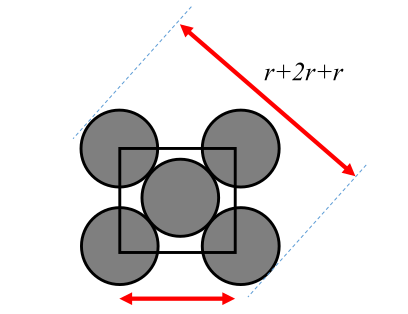
\includegraphics[width=0.7\textwidth]{images/cristallographie/cryst-005-000.png}
\caption{Schéma de réseau cristallin.}
\end{figure}

\begin{figure}[H]
\centering

\includegraphics[width=0.7\textwidth]{images/cristallographie/cryst-005-001.png}
\caption{Maille élémentaire et vecteurs de base.}
\end{figure}

\begin{figure}[H]
\centering
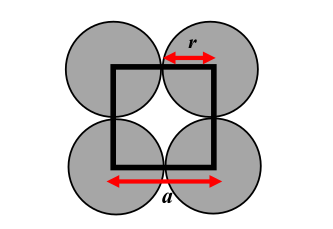
\includegraphics[width=0.7\textwidth]{images/cristallographie/cryst-006-002.png}
\caption{Structure cubique à faces centrées (CFC).}
\end{figure}

\begin{figure}[H]
\centering

\includegraphics[width=0.7\textwidth]{images/cristallographie/cryst-006-003.png}
\caption{Structure cubique centrée (CC).}
\end{figure}

\begin{figure}[H]
\centering
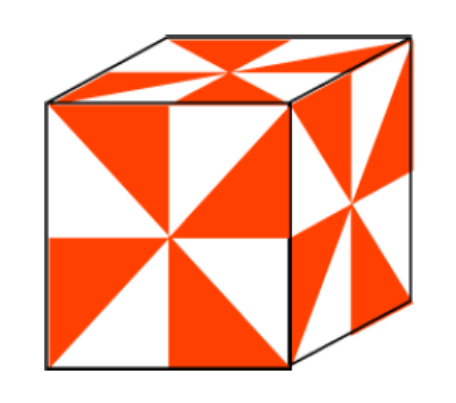
\includegraphics[width=0.7\textwidth]{images/cristallographie/cryst-010-004.png}
\caption{Indices de Miller d'un plan cristallin.}
\end{figure}

\begin{figure}[H]
\centering

\includegraphics[width=0.7\textwidth]{images/cristallographie/cryst-010-005.png}
\caption{Famille de plans réticulaires équivalents.}
\end{figure}

\begin{figure}[H]
\centering
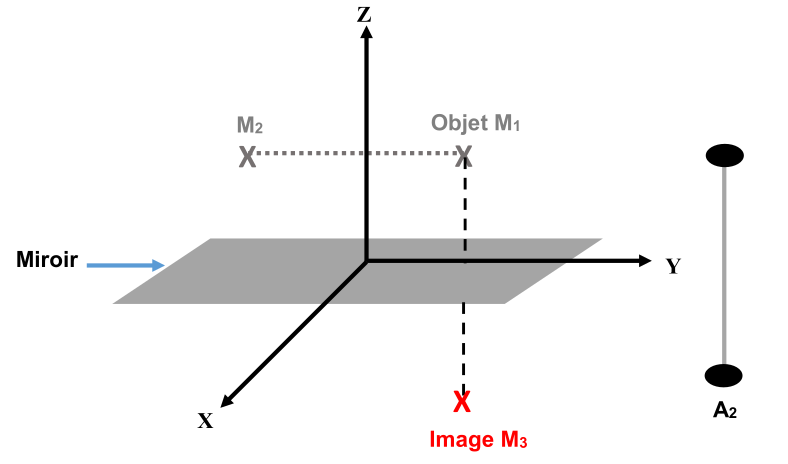
\includegraphics[width=0.7\textwidth]{images/cristallographie/cryst-011-006.png}
\caption{Loi de Bragg : diffraction des rayons X.}
\end{figure}

\begin{figure}[H]
\centering

\includegraphics[width=0.7\textwidth]{images/cristallographie/cryst-011-007.png}
\caption{Géométrie de la diffraction.}
\end{figure}

\begin{figure}[H]
\centering
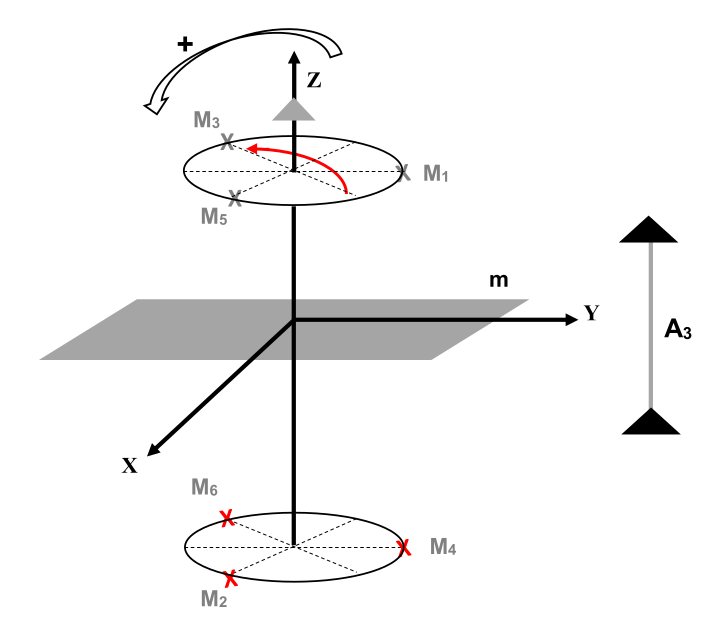
\includegraphics[width=0.7\textwidth]{images/cristallographie/cryst-012-008.png}
\caption{Réseau réciproque et vecteur de diffusion.}
\end{figure}

\begin{figure}[H]
\centering

\includegraphics[width=0.7\textwidth]{images/cristallographie/cryst-012-009.png}
\caption{Sphère d'Ewald et condition de diffraction.}
\end{figure}

\begin{figure}[H]
\centering
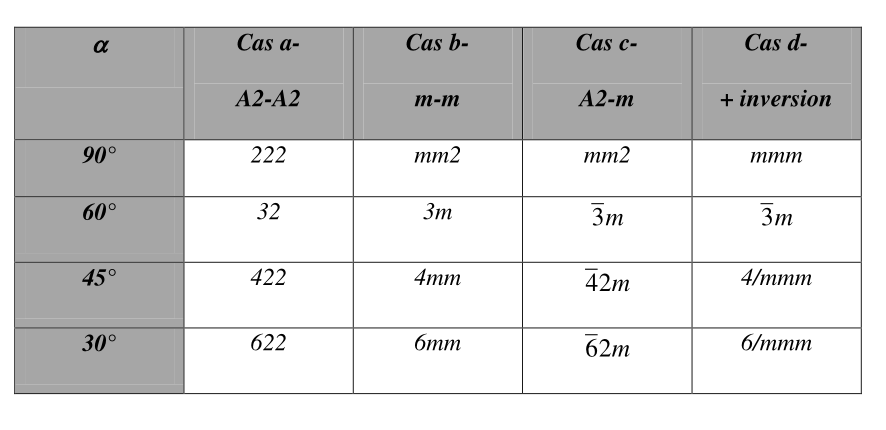
\includegraphics[width=0.7\textwidth]{images/cristallographie/cryst-013-010.png}
\caption{Structure NaCl : emboîtement de deux réseaux CFC.}
\end{figure}

\begin{figure}[H]
\centering

\includegraphics[width=0.7\textwidth]{images/cristallographie/cryst-013-011.png}
\caption{Sites interstitiels tétraédriques et octaédriques.}
\end{figure}

\begin{figure}[H]
\centering
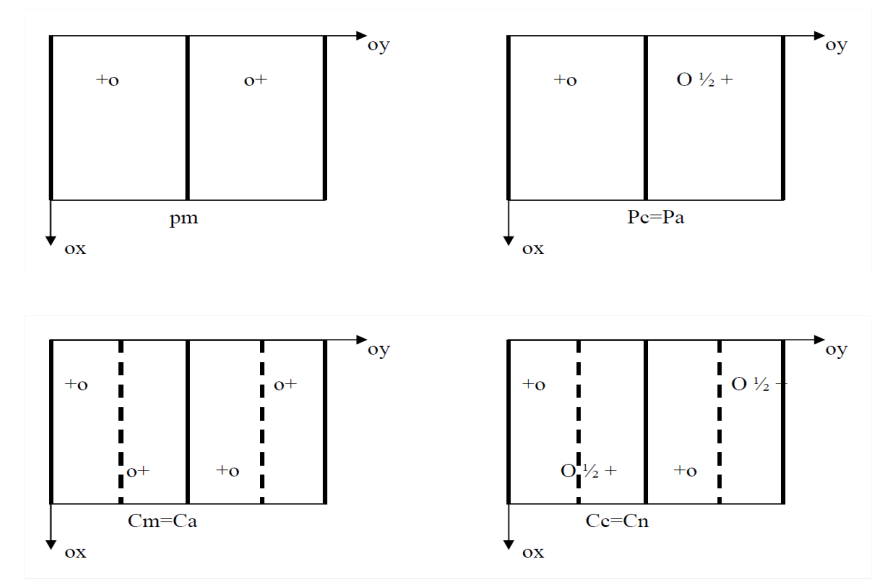
\includegraphics[width=0.7\textwidth]{images/cristallographie/cryst-014-012.png}
\caption{Structure hexagonale compacte (HC).}
\end{figure}

\begin{figure}[H]
\centering

\includegraphics[width=0.7\textwidth]{images/cristallographie/cryst-014-013.png}
\caption{Empilements compacts ABAB et ABCABC.}
\end{figure}

\ifdefined\inMainDoc\else\end{document}\fi


% ================================================================
%  UE 6 : ÉLECTROMAGNÉTISME DANS LA MATIÈRE
% ================================================================
\newpage
\thispagestyle{empty}
\begin{tikzpicture}[remember picture, overlay]
  \fill[gray!12] ([xshift=1.5cm, yshift=3cm]current page.south west)
    rectangle ([xshift=-1.5cm, yshift=-3cm]current page.north east);
  \draw[line width=3pt] ([xshift=1.5cm,yshift=-3cm]current page.north west)
    -- ([xshift=-1.5cm,yshift=-3cm]current page.north east);
  \draw[line width=3pt] ([xshift=1.5cm,yshift=3cm]current page.south west)
    -- ([xshift=-1.5cm,yshift=3cm]current page.south east);
  \node[align=center] at (current page.center) {%
    {\fontsize{24}{32}\bfseries\selectfont ÉLECTROMAGNÉTISME}\\[0.3cm]
    {\fontsize{24}{32}\bfseries\selectfont DANS LA MATIÈRE}\\[1.0cm]
    {\large\itshape Milieux diélectriques et magnétiques}\\[0.4cm]
    {\large\itshape Conditions aux interfaces}\\[1.5cm]
    {\normalsize Licence 3 - UE 6}
  };
  \node[anchor=south west] at ([xshift=2cm,yshift=2cm]current page.south west)
    {\large\bfseries UE 6};
\end{tikzpicture}
\newpage

\addcontentsline{toc}{section}{ÉLECTROMAGNÉTISME DANS LA MATIÈRE}
\ifdefined\inMainDoc\else
\documentclass[12pt,a4paper]{article}
% ================================================================
%  PRÉAMBULE COMMUN - ANNALES CORRIGÉES
%  Université de Kara - FaST - Licence Fondamentale MPC
%  Design optimisé impression noir et blanc
% ================================================================

% -- ENCODAGE & LANGUE --
\usepackage[utf8]{inputenc}
\usepackage[T1]{fontenc}
\usepackage[french]{babel}
\usepackage{lmodern}
\usepackage{microtype}

% -- MISE EN PAGE --
\usepackage[a4paper, top=2.8cm, bottom=2.5cm, left=2.5cm, right=2.5cm, headheight=14pt]{geometry}
\usepackage{setspace}
\setstretch{1.2}
\usepackage{parskip}
\setlength{\parindent}{1.2em}
\setlength{\parskip}{4pt}

% -- MATHS --
\usepackage{amsmath, amssymb, mathtools, amsthm}
\usepackage{mathrsfs}
\usepackage{dsfont}
\usepackage{bm}
\usepackage{cancel}
\usepackage{textcomp}
% Définition de \oiint (intégrale de surface fermée) sans package supplémentaire
\newcommand{\oiint}{\mathop{\iint\!\!\!\!\!\!\!\bigcirc}\limits}

% -- PHYSIQUE & CHIMIE --
\usepackage{physics}
\usepackage{siunitx}
% Lorsque physics est chargé, siunitx omet \qty. On le restaure ici :
\AtBeginDocument{\RenewCommandCopy\qty\SI}
\sisetup{locale = FR, detect-all, output-decimal-marker={,}}
% Commande de substitution pour les unités posant problème avec pdflatex
% (ohm, degreeCelsius, micro, angstrom, percent utilisent des caractères non-ASCII)
\newcommand{\qtyohm}[1]{\ensuremath{\num{#1}\,\Omega}}
\newcommand{\qtydegc}[1]{\ensuremath{\num{#1}\,{}^\circ\text{C}}}
\newcommand{\qtyangstrom}[1]{\ensuremath{\num{#1}\,\text{\AA}}}
\newcommand{\qtypercent}[1]{\ensuremath{\num{#1}\,\%}}
\newcommand{\qtyum}[1]{\ensuremath{\num{#1}\,\mu\text{m}}}
\usepackage[version=4]{mhchem}

% -- GRAPHISMES --
\usepackage{graphicx}
\usepackage{float}
\usepackage{caption}
\usepackage{subcaption}
\usepackage{wrapfig}
\usepackage{tikz}
\usetikzlibrary{calc, arrows.meta, patterns, shapes.geometric}
\usepackage{pgfplots}
\pgfplotsset{compat=1.18}

% -- TABLEAUX --
\usepackage{booktabs}
\usepackage{array}
\usepackage{tabularx}
\usepackage{multirow}

% -- LISTES --
\usepackage{enumitem}
\setlist[enumerate]{topsep=3pt, itemsep=2pt, parsep=0pt}
\setlist[itemize]{topsep=3pt, itemsep=2pt, parsep=0pt, label={.}}

% -- BOÎTES (noir et blanc) --
\usepackage{mdframed}
\usepackage{tcolorbox}
\tcbuselibrary{skins, breakable, theorems}

% Boîte EXERCICE : encadré avec filet épais, fond blanc
\newmdenv[
  linewidth=1.2pt,
  linecolor=black,
  roundcorner=3pt,
  skipabove=10pt,
  skipbelow=6pt,
  innertopmargin=8pt,
  innerbottommargin=8pt,
  innerleftmargin=10pt,
  innerrightmargin=10pt,
  backgroundcolor=white,
  frametitle={\bfseries\small Exercice},
  frametitlealignment=\raggedright,
  frametitleaboveskip=4pt,
  frametitlebelowskip=4pt,
]{boiteexercice}

% Boîte CORRIGÉ : fond gris très clair + filet fin
\newmdenv[
  linewidth=0.6pt,
  linecolor=black,
  leftline=true,
  rightline=false,
  topline=false,
  bottomline=false,
  linecolor=black,
  innerleftmargin=12pt,
  innerrightmargin=8pt,
  innertopmargin=6pt,
  innerbottommargin=6pt,
  backgroundcolor=gray!8,
  skipabove=4pt,
  skipbelow=8pt,
]{boitecorrige}

% Boîte RÉSUMÉ DE COURS : double encadré
\newmdenv[
  linewidth=0.8pt,
  linecolor=black,
  roundcorner=2pt,
  backgroundcolor=gray!12,
  innertopmargin=10pt,
  innerbottommargin=10pt,
  innerleftmargin=12pt,
  innerrightmargin=12pt,
  skipabove=12pt,
  skipbelow=8pt,
]{boiteresume}

% Boîte ATTENTION/REMARQUE : barre gauche épaisse
\newmdenv[
  leftline=true,
  rightline=false,
  topline=false,
  bottomline=false,
  linewidth=3pt,
  linecolor=black,
  backgroundcolor=gray!5,
  innerleftmargin=12pt,
  innerrightmargin=8pt,
  innertopmargin=5pt,
  innerbottommargin=5pt,
  skipabove=6pt,
  skipbelow=6pt,
]{boiteremarque}

% -- DIFFICULTÉ DES EXERCICES --
\newcommand{\facile}{$\star$}
\newcommand{\moyen}{$\star\!\star$}
\newcommand{\difficile}{$\star\!\star\!\star$}
\newcommand{\niveau}[1]{\hfill\textbf{#1}\hspace{2pt}}

% -- EN-TÊTES ET PIEDS DE PAGE --
\usepackage{fancyhdr}
\pagestyle{fancy}
\fancyhf{}
\renewcommand{\headrulewidth}{0.5pt}
\renewcommand{\footrulewidth}{0.3pt}

% -- HYPERLIENS --
\usepackage[hidelinks]{hyperref}
\hypersetup{
    colorlinks=false,
    pdftitle={Annale Corrigée - Licence MPC - Université de Kara}
}

% -- TITRES --
\usepackage{titlesec}
\titleformat{\section}{\Large\bfseries}{\thesection.}{0.8em}{}[\vspace{2pt}\hrule\vspace{4pt}]
\titleformat{\subsection}{\large\bfseries}{\thesubsection.}{0.7em}{}
\titleformat{\subsubsection}{\normalsize\bfseries}{\thesubsubsection.}{0.6em}{}

% -- THÉORÈMES --
\theoremstyle{definition}
\newtheorem{defn}{Définition}[section]
\newtheorem{prop}{Propriété}[section]
\newtheorem{thm}{Théorème}[section]
\newtheorem{corol}{Corollaire}[section]
\newtheorem{exemple}{Exemple}[section]

% -- COMMANDES MATHÉMATIQUES UTILES --
\newcommand{\vect}[1]{\overrightarrow{#1}}
\newcommand{\R}{\mathbb{R}}
\newcommand{\N}{\mathbb{N}}
\newcommand{\Z}{\mathbb{Z}}
\newcommand{\C}{\mathbb{C}}
\renewcommand{\d}{\mathrm{d}}
\newcommand{\deriv}[2]{\dfrac{\d #1}{\d #2}}
\newcommand{\dpart}[2]{\dfrac{\partial #1}{\partial #2}}
\newcommand{\rot}{\overrightarrow{\mathrm{rot}}\,}
\renewcommand{\div}{\mathrm{div}\,}
\renewcommand{\grad}{\overrightarrow{\mathrm{grad}}\,}
\newcommand{\e}{\mathrm{e}}
\newcommand{\ii}{\mathrm{i}}
\renewcommand{\Tr}{\mathrm{Tr}}

% Numérotation des équations par section
\numberwithin{equation}{section}

% -- RÉSULTATS ENCADRÉS --
\newcommand{\res}[1]{\[\boxed{#1}\]}

% -- REMARQUE INLINE --
\newcommand{\rmq}[1]{\begin{boiteremarque}\textbf{Remarque.} #1\end{boiteremarque}}

% -- MISE EN VALEUR DU RÉSULTAT FINAL --
\newcommand{\reponse}[1]{%
  \begin{center}
    \fbox{\begin{minipage}{0.92\textwidth}\centering #1\end{minipage}}
  \end{center}%
}


\lhead{\small\textit{Électromagnétisme dans la Matière - Licence 3}}
\rhead{\small\textit{FaST, Université de Kara}}
\cfoot{\thepage}

\begin{document}
\fi

\begin{center}
  {\LARGE\bfseries ÉLECTROMAGNÉTISME DANS LA MATIÈRE}\\[0.3cm]
  {\normalsize Licence 3 - Physique}\\[0.1cm]
  \rule{0.7\textwidth}{0.8pt}
\end{center}

\section*{Résumé du cours}

\begin{boiteresume}

\textbf{1. Polarisation diélectrique.}
Dans un diélectrique LHI (linéaire, homogène, isotrope), les dipôles microscopiques créent une polarisation macroscopique $\vec{P} = \epsilon_0\chi_e\vec{E}$, avec $\chi_e = \epsilon_r-1$ la susceptibilité électrique. Le vecteur déplacement électrique est :
\[
\vec{D} = \epsilon_0\vec{E} + \vec{P} = \epsilon_0\epsilon_r\vec{E}.
\]
Les charges de polarisation volumiques et surfaciques sont $\rho_p = -\div\vec{P}$ et $\sigma_p = \vec{P}\cdot\hat{n}$.

\textbf{2. Champ local (relation de Clausius-Mossotti).}
Pour un diélectrique, le champ local ressenti par un dipôle est :
\[
\vec{E}_\text{loc} = \vec{E} + \frac{\vec{P}}{3\epsilon_0},
\]
ce qui conduit, pour une polarisabilité atomique $\alpha$, à la relation de Clausius-Mossotti :
$\dfrac{\epsilon_r-1}{\epsilon_r+2} = \dfrac{n\alpha}{3\epsilon_0}$, où $n$ est la densité de dipôles.

\textbf{3. Magnétisation.}
Dans un milieu magnétique LHI, $\vec{M} = \chi_m\vec{H}$ avec $\chi_m$ la susceptibilité magnétique. Le champ $\vec{B}$ et le vecteur excitation $\vec{H}$ sont liés par :
\[
\vec{B} = \mu_0(\vec{H}+\vec{M}) = \mu_0\mu_r\vec{H}.
\]
Les courants d'aimantation volumiques et surfaciques sont $\vec{j}_m = \rot\vec{M}$ et $\vec{K}_m = \vec{M}\times\hat{n}$.

\textbf{4. Équations de Maxwell dans la matière.}
\[
\div\vec{D} = \rho_\ell, \quad
\div\vec{B} = 0, \quad
\rot\vec{E} = -\frac{\partial\vec{B}}{\partial t}, \quad
\rot\vec{H} = \vec{j}_\ell + \frac{\partial\vec{D}}{\partial t}.
\]

\textbf{5. Conditions aux limites à une interface.}
Pour une interface entre deux milieux (1) et (2), avec la normale $\hat{n}$ de (1) vers (2) :
\[
(D_2-D_1)\cdot\hat{n} = \sigma_\ell, \quad
(B_2-B_1)\cdot\hat{n} = 0, \quad
(E_2-E_1)\times\hat{n} = \vec{0}, \quad
(H_2-H_1)\times\hat{n} = \vec{K}_\ell.
\]
En l'absence de charges et courants libres surfaciques : la composante normale de $\vec{D}$ et la composante tangentielle de $\vec{E}$ sont continues.

\textbf{6. Ondes électromagnétiques dans les milieux matériels.}
Dans un milieu LHI non absorbant d'indices $\epsilon_r$ et $\mu_r$, l'onde plane se propage avec la vitesse $v = c/n$, où l'indice de réfraction vaut $n = \sqrt{\epsilon_r\mu_r}$. En présence d'absorption, $n$ devient complexe : $\tilde{n} = n + \ii\kappa$ (avec $\kappa$ le coefficient d'extinction). L'intensité décroît en $\e^{-2\kappa\omega z/c}$ (loi de Beer-Lambert). À une interface, les lois de Snell-Descartes s'appliquent : $n_1\sin\theta_1 = n_2\sin\theta_2$.

\end{boiteresume}

\newpage
\subsection*{Exercice 1 - Champ local dans un diélectrique \niveau{\moyen}}

\begin{boiteexercice}
On considère un diélectrique LHI de polarisation uniforme $\vec{P}$ dans un champ extérieur $\vec{E}_0$. On creuse une cavité sphérique de rayon $R$ (très petit à l'échelle macroscopique) centrée sur un point $M$ du diélectrique.
\begin{enumerate}
  \item Exprimer le champ local $\vec{E}_\text{loc}$ en $M$ en fonction du champ macroscopique $\vec{E}$ et du champ $\vec{E}_p'(M)$ créé par les charges de polarisation sur la surface $S'$ de la cavité.
  \item Calculer $\vec{E}_p'(M)$ en fonction de $\vec{P}$ et $\epsilon_0$. En déduire $\vec{E}_\text{loc}$ en fonction de $\vec{P}$, $\epsilon_0$ et $\vec{E}$.
\end{enumerate}
\end{boiteexercice}

\begin{boitecorrige}

\textbf{1. Expression du champ local.}

Le champ en $M$ résulte de trois contributions :
\[
\vec{E}_\text{loc} = \vec{E}_0 + \vec{E}_p + \vec{E}_p',
\]
où $\vec{E}_p$ est le champ créé par les charges de polarisation sur la surface extérieure $S$ du diélectrique, et $\vec{E}_p'$ est celui créé par les charges sur la surface $S'$ de la cavité. Or $\vec{E}_0 + \vec{E}_p = \vec{E}$ (champ macroscopique), d'où :
\[
\vec{E}_\text{loc} = \vec{E} + \vec{E}_p'.
\]

\textbf{2. Calcul de $\vec{E}_p'$.}

La densité surfacique de charges de polarisation sur $S'$ est $\sigma_p = \vec{P}\cdot(-\hat{e}_r) = -P\cos\theta$ (la normale extérieure à la cavité est $-\hat{e}_r$). Le champ élémentaire en $M$ créé par un élément de surface $\d S' = 2\pi R^2\sin\theta\,\d\theta$ est, par la loi de Coulomb :
\[
\d\vec{E}_p' = \frac{1}{4\pi\epsilon_0}\,\frac{\sigma_p\,\d S'}{R^2}\,(-\hat{e}_r).
\]
Par symétrie de révolution autour de l'axe $\vec{P}$, seule la composante sur cet axe subsiste :
\[
E_{p,z}' = \frac{P}{2\epsilon_0}\int_0^{\pi}\cos^2\theta\sin\theta\,\d\theta
= \frac{P}{2\epsilon_0}\cdot\frac{2}{3} = \frac{P}{3\epsilon_0}.
\]
Donc :
\[
\vec{E}_p' = \frac{\vec{P}}{3\epsilon_0},
\qquad\text{et}\qquad
\boxed{\vec{E}_\text{loc} = \vec{E} + \frac{\vec{P}}{3\epsilon_0}.}
\]
Ce résultat est la \emph{relation de Lorentz} pour le champ local.
\end{boitecorrige}

\subsection*{Exercice 2 - Condensateur plan avec deux diélectriques en parallèle \niveau{\moyen}}

\begin{boiteexercice}
Un condensateur plan est formé de deux plaques rectangulaires de dimensions $(a, e)$ séparées d'une distance $d$. Il porte une distribution surfacique de charges libres $\sigma_\ell$. On néglige les effets de bord.
\begin{enumerate}
  \item Condensateur à air. Calculer le champ électrique entre les armatures et la capacité $C_0$.
  \item Le condensateur est maintenant rempli de deux diélectriques de permittivités relatives $\epsilon_{r1}$ et $\epsilon_{r2}$, disposés en parallèle sur des longueurs $e_1$ et $e_2$ respectivement ($e_1+e_2=e$).
  \begin{enumerate}[label=\alph*)]
    \item Calculer les champs $\vec{D}_i$ et $\vec{E}_i$ dans chaque diélectrique $i$.
    \item En déduire une relation entre la densité de charges libres $\sigma_\ell$ et la densité de charges de polarisation $\sigma_p^i$ dans le diélectrique $i$.
    \item Calculer la nouvelle capacité $C$ en fonction de $a$, $e_1$, $e_2$, $d$, $\epsilon_{r1}$ et $\epsilon_{r2}$. Conclure.
    \item Que vaut $C$ si les deux diélectriques sont identiques ?
  \end{enumerate}
\end{enumerate}
\end{boiteexercice}

\begin{boitecorrige}

\textbf{1. Condensateur à air.}

Par le théorème de Gauss, chaque armature crée $\sigma_\ell/(2\epsilon_0)$. Les deux contributions s'ajoutent entre les armatures :
\[
\vec{E}_0 = \frac{\sigma_\ell}{\epsilon_0}\,\hat{e}_z.
\]
La tension est $U_0 = E_0\,d$, et la capacité :
\[
C_0 = \frac{Q_\ell}{U_0} = \frac{\sigma_\ell\,ae}{E_0\,d} = \frac{\epsilon_0\,ae}{d}.
\]

\textbf{2. Avec deux diélectriques en parallèle.}

\textbf{a)} Les diélectriques étant disposés parallèlement aux armatures (même tension à leurs bornes), la continuité de la composante normale de $\vec{D}$ à l'interface armature/diélectrique donne :
\[
\vec{D}_i = \sigma_\ell\,\hat{e}_z
\qquad\Rightarrow\qquad
\vec{E}_i = \frac{\vec{D}_i}{\epsilon_0\epsilon_{ri}} = \frac{\sigma_\ell}{\epsilon_0\epsilon_{ri}}\,\hat{e}_z.
\]

\textbf{b)} La polarisation dans le diélectrique $i$ est $\vec{P}_i = (\epsilon_{ri}-1)\epsilon_0\vec{E}_i = \left(1-\dfrac{1}{\epsilon_{ri}}\right)\sigma_\ell\,\hat{e}_z$.

La charge de polarisation surfacique à l'interface avec l'armature est $\sigma_p^i = P_i\cdot(-1)$ (normale sortante opposée) :
\[
\sigma_p^i = -\left(1 - \frac{1}{\epsilon_{ri}}\right)\sigma_\ell = \left(\frac{1}{\epsilon_{ri}}-1\right)\sigma_\ell.
\]

\textbf{c)} Le système est équivalent à deux condensateurs en parallèle, chacun de surface $ae_i$ et de distance $d$. La capacité totale est :
\[
C = C_1 + C_2 = \frac{\epsilon_0\epsilon_{r1}\,ae_1}{d} + \frac{\epsilon_0\epsilon_{r2}\,ae_2}{d}
= \frac{\epsilon_0\,a}{d}\!\left(\epsilon_{r1}\,e_1+\epsilon_{r2}\,e_2\right).
\]
Deux condensateurs en parallèle ont la même tension à leurs bornes et leurs capacités s'additionnent.

\textbf{d)} Si $\epsilon_{r1}=\epsilon_{r2}=\epsilon_r$, alors $e_1+e_2=e$ et :
\[
C = \frac{\epsilon_0\epsilon_r\,ae}{d} = \epsilon_r C_0.
\]
On retrouve bien que remplir un condensateur d'un diélectrique uniforme multiplie sa capacité par $\epsilon_r$.

\end{boitecorrige}

\subsection*{Exercice 3 - Réfraction à l'interface entre deux diélectriques \niveau{\moyen}}

\begin{boiteexercice}
Une onde électromagnétique plane se propage dans le vide et atteint une interface plane avec un diélectrique de permittivité relative $\epsilon_r = 4$ (milieu non magnétique). L'angle d'incidence est $\theta_i = 30°$.
\begin{enumerate}
  \item Calculer l'indice de réfraction $n$ du diélectrique.
  \item Appliquer la loi de Snell-Descartes pour trouver l'angle de réfraction $\theta_r$.
  \item Existe-t-il un angle de Brewster pour une polarisation TM ? Si oui, le calculer.
\end{enumerate}
\end{boiteexercice}

\begin{boitecorrige}

\textbf{1.} Pour un milieu non magnétique ($\mu_r=1$) : $n = \sqrt{\epsilon_r} = \sqrt{4} = 2$.

\textbf{2.} La loi de Snell-Descartes donne ($n_1=1$ pour le vide, $n_2=2$) :
\[
n_1\sin\theta_i = n_2\sin\theta_r \implies \sin\theta_r = \frac{\sin 30°}{2} = \frac{1}{4}
\implies \theta_r = \arcsin\!\left(\frac{1}{4}\right) \approx 14{,}5°.
\]

\textbf{3.} L'angle de Brewster $\theta_B$ pour la polarisation TM vérifie $\tan\theta_B = n_2/n_1 = 2$, soit :
\[
\theta_B = \arctan(2) \approx 63{,}4°.
\]
À cet angle d'incidence, la composante TM du champ réfléchi s'annule.
\end{boitecorrige}

\subsection*{Exercice 4 - Conditions aux limites magnétiques \niveau{\moyen}}

\begin{boiteexercice}
On considère une interface plane séparant deux milieux magnétiques LHI de perméabilités relatives $\mu_{r1}$ et $\mu_{r2}$. Un champ $\vec{B}_1$ fait un angle $\alpha_1$ avec la normale à l'interface dans le milieu 1.
\begin{enumerate}
  \item Écrire les conditions aux limites sur $\vec{B}$ et $\vec{H}$ à l'interface (en l'absence de courant surfacique libre).
  \item Établir la loi de réfraction du champ magnétique : $\dfrac{\tan\alpha_1}{\tan\alpha_2} = \dfrac{\mu_{r1}}{\mu_{r2}}$.
\end{enumerate}
\end{boiteexercice}

\begin{boitecorrige}

\textbf{1. Conditions aux limites.}

En l'absence de courant surfacique libre, les conditions aux limites sont :
\begin{align*}
B_{2n} &= B_{1n} \quad\text{(composante normale de $\vec{B}$, continue)}\\
H_{2t} &= H_{1t} \quad\text{(composante tangentielle de $\vec{H}$, continue)}
\end{align*}

\textbf{2. Loi de réfraction.}

Les composantes sont :
\[
B_{1n} = B_1\cos\alpha_1,\quad B_{1t} = B_1\sin\alpha_1,\quad H_{1t} = \frac{B_{1t}}{\mu_0\mu_{r1}} = \frac{B_1\sin\alpha_1}{\mu_0\mu_{r1}}.
\]
La continuité de $B_n$ donne $B_1\cos\alpha_1 = B_2\cos\alpha_2$.

La continuité de $H_t$ donne $\dfrac{B_1\sin\alpha_1}{\mu_{r1}} = \dfrac{B_2\sin\alpha_2}{\mu_{r2}}$.

En divisant la seconde équation par la première :
\[
\frac{\tan\alpha_1}{\mu_{r1}} = \frac{\tan\alpha_2}{\mu_{r2}}
\implies \boxed{\frac{\tan\alpha_1}{\tan\alpha_2} = \frac{\mu_{r1}}{\mu_{r2}}.}
\]
\end{boitecorrige}

\subsection*{Exercice 5 - Onde électromagnétique dans un milieu absorbant \niveau{\difficile}}

\begin{boiteexercice}
On considère une onde électromagnétique plane de pulsation $\omega$ se propageant dans un milieu conducteur de permittivité $\epsilon_r$, de perméabilité $\mu_r = 1$ et de conductivité $\sigma$.
\begin{enumerate}
  \item Montrer que l'équation de propagation pour le champ $\vec{E}$ s'écrit :
  \[
    \Delta\vec{E} = \mu_0\epsilon_0\epsilon_r\frac{\partial^2\vec{E}}{\partial t^2} + \mu_0\sigma\frac{\partial\vec{E}}{\partial t}.
  \]
  \item En cherchant une solution en onde plane $\vec{E} = \vec{E}_0\,\e^{\ii(\tilde{k}z-\omega t)}$, montrer que le vecteur d'onde complexe vérifie $\tilde{k}^2 = \mu_0\epsilon_0\omega^2\!\left(\epsilon_r + \dfrac{\ii\sigma}{\epsilon_0\omega}\right)$.
  \item Identifier la profondeur de peau $\delta$ (distance de pénétration) dans la limite des bons conducteurs ($\sigma\gg\epsilon_0\epsilon_r\omega$).
\end{enumerate}
\end{boiteexercice}

\begin{boitecorrige}

\textbf{1. Équation de propagation.}

La loi d'Ohm donne $\vec{j} = \sigma\vec{E}$. Les équations de Maxwell dans le milieu ($\div\vec{E}=0$ pour une onde transverse) donnent :
\[
\rot(\rot\vec{E}) = -\nabla^2\vec{E} = -\mu_0\frac{\partial}{\partial t}(\rot\vec{H}) = -\mu_0\frac{\partial}{\partial t}\!\left(\sigma\vec{E}+\epsilon_0\epsilon_r\frac{\partial\vec{E}}{\partial t}\right).
\]
D'où l'équation de propagation :
\[
\Delta\vec{E} = \mu_0\epsilon_0\epsilon_r\frac{\partial^2\vec{E}}{\partial t^2} + \mu_0\sigma\frac{\partial\vec{E}}{\partial t}.
\]

\textbf{2. Relation de dispersion.}

En substituant $\vec{E} = \vec{E}_0\,\e^{\ii(\tilde{k}z-\omega t)}$, on obtient $-\tilde{k}^2 = -\mu_0\epsilon_0\epsilon_r\omega^2 + \ii\mu_0\sigma\omega$, soit :
\[
\tilde{k}^2 = \mu_0\epsilon_0\omega^2\!\left(\epsilon_r + \frac{\ii\sigma}{\epsilon_0\omega}\right).
\]
C'est la permittivité complexe $\tilde{\epsilon}_r = \epsilon_r + \ii\sigma/(\epsilon_0\omega)$.

\textbf{3. Profondeur de peau.}

Dans la limite $\sigma\gg\epsilon_0\epsilon_r\omega$ (bon conducteur) :
\[
\tilde{k}^2 \approx \ii\mu_0\sigma\omega
\implies \tilde{k} \approx \frac{1+\ii}{\sqrt{2}}\sqrt{\mu_0\sigma\omega}.
\]
La partie imaginaire donne l'amortissement : l'amplitude décroît comme $\e^{-\Im(\tilde{k})z}$. La profondeur de peau est :
\[
\boxed{\delta = \frac{1}{\Im(\tilde{k})} = \sqrt{\frac{2}{\mu_0\sigma\omega}}.}
\]
L'onde est atténuée d'un facteur $1/e$ sur une distance $\delta$. Pour le cuivre à $50\;\text{Hz}$, $\delta\approx 9\;\text{mm}$.

\end{boitecorrige}

\subsection*{Exercice 6 - Énergie électromagnétique dans un diélectrique \niveau{\moyen}}

\begin{boiteexercice}
Un condensateur plan de surface $S$ et de distance $d$ est rempli d'un diélectrique de permittivité $\epsilon_r$. Il est chargé sous une tension $U$.
\begin{enumerate}
  \item Calculer l'énergie électrostatique stockée.
  \item Calculer la densité d'énergie électromagnétique dans le diélectrique.
  \item Exprimer la force exercée sur le diélectrique si on l'introduit progressivement entre les armatures, à charge constante.
\end{enumerate}
\end{boiteexercice}

\begin{boitecorrige}

\textbf{1.} La capacité est $C = \epsilon_0\epsilon_r S/d$ et l'énergie stockée :
\[
W = \frac{1}{2}CU^2 = \frac{\epsilon_0\epsilon_r S U^2}{2d}.
\]

\textbf{2.} Le champ entre les armatures est $E = U/d$. La densité d'énergie dans le diélectrique est :
\[
u_e = \frac{1}{2}\vec{D}\cdot\vec{E} = \frac{1}{2}\epsilon_0\epsilon_r E^2 = \frac{\epsilon_0\epsilon_r U^2}{2d^2}.
\]
On vérifie bien que $W = u_e\cdot Sd$.

\textbf{3.} À charge $Q$ constante, l'énergie est $W = Q^2/(2C)$. En notant $x$ la fraction du condensateur remplie par le diélectrique (longueur $x$ sur la longueur totale $L$) :
\[
C(x) = \frac{\epsilon_0 S}{d}\!\left[\epsilon_r\,\frac{x}{L} + 1\cdot\frac{L-x}{L}\right] = C_0\!\left[1 + (\epsilon_r-1)\frac{x}{L}\right].
\]
La force est :
\[
F = -\frac{\partial W}{\partial x}\Bigg|_Q = \frac{Q^2}{2C^2}\frac{\partial C}{\partial x} = \frac{Q^2(\epsilon_r-1)}{2C_0 L}\cdot\frac{C_0^2}{C^2} \cdot \frac{\d C}{\d x}.
\]
Le diélectrique est aspiré vers l'intérieur du condensateur ($\epsilon_r > 1$, donc $F > 0$ dans le sens d'insertion) car cela diminue l'énergie à charge constante.

\end{boitecorrige}

\subsection*{Exercice 7 - Sphère diélectrique dans un champ uniforme \niveau{\difficile}}

\begin{boiteexercice}
Une sphère de rayon $R$, constituée d'un diélectrique LHI de permittivité relative $\epsilon_r$, est plongée dans un champ électrostatique uniforme $\vec{E}_0 = E_0\,\hat{e}_z$ dans le vide.
\begin{enumerate}
  \item Déterminer le potentiel $V_1$ à l'intérieur de la sphère et $V_2$ à l'extérieur, en cherchant des solutions à symétrie axiale de la forme $V(r,\theta) = \sum_l (A_l r^l + B_l r^{-(l+1)})P_l(\cos\theta)$.
  \item Exprimer le champ électrique $\vec{E}_\text{int}$ à l'intérieur de la sphère.
  \item Calculer la polarisation $\vec{P}$ et la densité surfacique de charges de polarisation $\sigma_p$.
\end{enumerate}
\end{boiteexercice}

\begin{boitecorrige}

\textbf{1. Potentiel à l'intérieur et à l'extérieur.}

À l'extérieur, le potentiel doit tendre vers $-E_0 r\cos\theta$ (champ uniforme) lorsque $r\to\infty$. À l'intérieur, il doit être fini en $r=0$. On conserve uniquement le terme $l=1$ :
\[
V_1(r,\theta) = -A\,r\cos\theta \quad (r<R),\qquad V_2(r,\theta) = -E_0\,r\cos\theta + \frac{B\cos\theta}{r^2} \quad (r>R).
\]
Les conditions aux limites à $r=R$ sont la continuité du potentiel et celle de la composante normale de $\vec{D} = \epsilon_0\epsilon_r\vec{E}$ :
\begin{align*}
V_1(R,\theta) &= V_2(R,\theta) \quad\Rightarrow\quad -AR = -E_0 R + B/R^2,\\
\epsilon_r\,\frac{\partial V_1}{\partial r}\Big|_R &= \frac{\partial V_2}{\partial r}\Big|_R \quad\Rightarrow\quad -\epsilon_r A = -E_0 - 2B/R^3.
\end{align*}
La résolution donne :
\[
A = \frac{3E_0}{\epsilon_r+2}, \qquad B = R^3 E_0\,\frac{\epsilon_r-1}{\epsilon_r+2}.
\]

\textbf{2. Champ intérieur.}

Le potentiel $V_1 = -A\,z$ correspond à un champ uniforme :
\[
\vec{E}_\text{int} = A\,\hat{e}_z = \frac{3}{\epsilon_r+2}\,\vec{E}_0.
\]
Le champ à l'intérieur est donc uniforme et réduit par le facteur $3/(\epsilon_r+2)$ : c'est le \emph{champ dépolarisant}.

\textbf{3. Polarisation et charges de polarisation.}

La polarisation est uniforme :
\[
\vec{P} = \epsilon_0(\epsilon_r-1)\vec{E}_\text{int} = 3\epsilon_0\,\frac{\epsilon_r-1}{\epsilon_r+2}\,\vec{E}_0.
\]
La densité surfacique de charges de polarisation est $\sigma_p = \vec{P}\cdot\hat{n} = P\cos\theta$, soit une distribution dipolaire surfacique. Le moment dipolaire total vaut $\vec{p} = \vec{P}\cdot(4\pi R^3/3)$, qui co\"incide avec le dipôle équivalent au champ extérieur ($B = p/(4\pi\epsilon_0)$).

\reponse{$\vec{E}_\text{int} = \dfrac{3}{\epsilon_r+2}\,\vec{E}_0$}
\end{boitecorrige}

\subsection*{Exercice 8 - Solénoïde torique à noyau ferromagnétique \niveau{\moyen}}

\begin{boiteexercice}
Un solénoïde torique de rayon moyen $R$ et de section circulaire de rayon $a\ll R$ comporte $N$ spires. Il est bobiné autour d'un noyau ferromagnétique de perméabilité $\mu_r = 1000$.
\begin{enumerate}
  \item Déterminer le champ $\vec{H}$, puis $\vec{B}$ à l'intérieur du tore en fonction du courant $I$.
  \item Calculer l'inductance $L$ de la bobine.
  \item On ouvre une mince fente d'épaisseur $e\ll 2\pi R$ dans le tore. En supposant que $\vec{B}$ reste tangentiel et continu, calculer le nouveau champ $H_\text{fer}$ dans le fer et $H_\text{air}$ dans la fente. Conclure.
\end{enumerate}
\end{boiteexercice}

\begin{boitecorrige}

\textbf{1. Champ dans le tore.}

Par symétrie, on applique le théorème d'Ampère sur un cercle de rayon $R$ :
\[
\oint \vec{H}\cdot\d\vec{\ell} = H\cdot 2\pi R = NI \quad\Rightarrow\quad H = \frac{NI}{2\pi R}.
\]
Le champ $B$ vaut alors :
\[
B = \mu_0\mu_r H = \frac{\mu_0\mu_r N I}{2\pi R}.
\]

\textbf{2. Inductance.}

Le flux à travers une spire est $\Phi_\text{spire} = B\cdot\pi a^2$. Le flux total pour $N$ spires :
\[
\Phi = N\Phi_\text{spire} = \frac{\mu_0\mu_r N^2 \pi a^2 I}{2\pi R}.
\]
L'inductance est $L = \Phi/I$, soit :
\[
L = \frac{\mu_0\mu_r N^2 a^2}{2R}.
\]

\textbf{3. Fente d'air.}

La continuité de la composante normale de $\vec{B}$ donne $B_\text{fer} = B_\text{air} = B$. En revanche, $H$ est discontinu :
\[
H_\text{fer} = \frac{B}{\mu_0\mu_r}, \qquad H_\text{air} = \frac{B}{\mu_0}.
\]
Le théorème d'Ampère devient :
\[
NI = H_\text{fer}(2\pi R - e) + H_\text{air}\,e = \frac{B}{\mu_0}\!\left[\frac{2\pi R - e}{\mu_r} + e\right].
\]
Comme $e\ll 2\pi R$ mais $\mu_r\gg 1$, le terme $e$ peut dominer. Par exemple pour $\mu_r = 1000$ et $e/(2\pi R) = 10^{-3}$, le rapport des champs vaut $H_\text{air}/H_\text{fer} = \mu_r$, et la fente d'air \emph{« désaimante »} fortement le noyau : le champ $B$ chute d'un facteur $\approx 2$. C'est pourquoi les circuits magnétiques réels doivent avoir des entrefers les plus courts possibles.

\reponse{$L = \dfrac{\mu_0\mu_r N^2 a^2}{2R}$}
\end{boitecorrige}

\subsection*{Exercice 9 - Capacité d'un câble coaxial à deux diélectriques \niveau{\moyen}}

\begin{boiteexercice}
Un câble coaxial est constitué d'un conducteur interne de rayon $a$ et d'une gaine externe de rayon interne $b$. L'espace entre les conducteurs est partiellement rempli de deux diélectriques concentriques : un diélectrique de permittivité $\epsilon_1$ entre $a$ et $c$ (avec $a<c<b$), et un diélectrique $\epsilon_2$ entre $c$ et $b$. La longueur du câble est $\ell$.
\begin{enumerate}
  \item Déterminer $\vec{D}$, $\vec{E}_1$ et $\vec{E}_2$ pour une charge $\lambda$ par unité de longueur.
  \item Calculer la ddp $U$ entre les conducteurs.
  \item En déduire la capacité par unité de longueur $C/\ell$.
\end{enumerate}
\end{boiteexercice}

\begin{boitecorrige}

\textbf{1. Champs.}

Par symétrie cylindrique, $\vec{D} = D(r)\hat{e}_r$. Le théorème de Gauss sur un cylindre de rayon $r$ ($a<r<b$) et de longueur $\ell$ :
\[
\oint \vec{D}\cdot\d\vec{S} = D\cdot 2\pi r \ell = \lambda \ell \quad\Rightarrow\quad \vec{D} = \frac{\lambda}{2\pi r}\hat{e}_r.
\]
Les champs électriques dans chaque diélectrique :
\[
\vec{E}_1 = \frac{\lambda}{2\pi\epsilon_1 r}\hat{e}_r \;(a<r<c), \qquad \vec{E}_2 = \frac{\lambda}{2\pi\epsilon_2 r}\hat{e}_r \;(c<r<b).
\]

\textbf{2. Différence de potentiel.}

\[
U = \int_a^b E(r)\,\d r = \int_a^c \frac{\lambda\,\d r}{2\pi\epsilon_1 r} + \int_c^b \frac{\lambda\,\d r}{2\pi\epsilon_2 r} = \frac{\lambda}{2\pi}\!\left[\frac{\ln(c/a)}{\epsilon_1} + \frac{\ln(b/c)}{\epsilon_2}\right].
\]

\textbf{3. Capacité linéique.}

\[
\frac{C}{\ell} = \frac{\lambda}{U} = \frac{2\pi}{\dfrac{\ln(c/a)}{\epsilon_1} + \dfrac{\ln(b/c)}{\epsilon_2}}.
\]
Les deux diélectriques en série s'additionnent comme des capacités en série. Pour $\epsilon_1 = \epsilon_2 = \epsilon$, on retrouve $C/\ell = 2\pi\epsilon/\ln(b/a)$.

\reponse{$C/\ell = \dfrac{2\pi}{\dfrac{1}{\epsilon_1}\ln\dfrac{c}{a} + \dfrac{1}{\epsilon_2}\ln\dfrac{b}{c}}$}
\end{boitecorrige}

\subsection*{Exercice 10 - Pression de radiation sur un miroir parfait \niveau{\moyen}}

\begin{boiteexercice}
Une onde électromagnétique plane progressive monochromatique d'intensité $I$ (en $\text{W\,m}^{-2}$) arrive normalement sur un miroir parfaitement conducteur (réflectivité $R=1$).
\begin{enumerate}
  \item Rappeler la relation entre $I$ et le module du vecteur de Poynting moyen $\langle\Pi\rangle$.
  \item Calculer la pression de radiation $P_\text{rad}$ exercée sur le miroir par transfert de quantité de mouvement.
  \item Application : un laser de puissance $1\;\text{kW}$ focalisé sur $1\;\text{mm}^2$. Calculer $P_\text{rad}$.
\end{enumerate}
\end{boiteexercice}

\begin{boitecorrige}

\textbf{1. Intensité.}

Pour une onde plane dans le vide, $\vec{E} = E_0\cos(kz-\omega t)\hat{e}_x$, $\vec{B} = E_0/c\cos(kz-\omega t)\hat{e}_y$. Le vecteur de Poynting vaut :
\[
\vec{\Pi} = \frac{\vec{E}\times\vec{B}}{\mu_0} = \frac{E_0^2}{\mu_0 c}\cos^2(kz-\omega t)\,\hat{e}_z.
\]
En moyenne temporelle $\langle\cos^2\rangle = 1/2$, donc :
\[
I = \langle\Pi\rangle = \frac{E_0^2}{2\mu_0 c}.
\]

\textbf{2. Pression de radiation.}

Le miroir parfait réfléchit l'onde : la quantité de mouvement par photon passe de $+p$ à $-p$, soit une variation $\Delta p = 2p$. Pour $n$ photons par unité de volume et de temps, le flux de quantité de mouvement réfléchi est $2I/c$. La pression de radiation est donc :
\[
P_\text{rad} = \frac{2I}{c}.
\]

\textbf{3. Application.}

Pour $P_\text{laser} = 1\;\text{kW}$ sur $S = 1\;\text{mm}^2 = 10^{-6}\;\text{m}^2$ :
\[
I = \frac{10^3}{10^{-6}} = 10^9\;\text{W\,m}^{-2}, \qquad P_\text{rad} = \frac{2\times 10^9}{3\times 10^8} \approx 6{,}67\;\text{Pa}.
\]
Soit une force $F = P_\text{rad}\cdot S \approx 6{,}67\;\mu\text{N}$.

\reponse{$P_\text{rad} = \dfrac{2I}{c}$}
\end{boitecorrige}

\subsection*{Exercice 11 - Théorème de Clausius-Mossotti pour les gaz \niveau{\moyen}}

\begin{boiteexercice}
On considère un gaz de molécules polaires de moment dipolaire permanent $p_0$, à la température $T$ et de densité volumique $n$.
\begin{enumerate}
  \item Établir la polarisation moyenne de Langevin $\langle p_z\rangle = p_0\mathcal{L}(\beta)$ avec $\beta = p_0 E/(k_B T)$.
  \item Dans la limite $\beta\ll 1$, montrer que la permittivité relative suit la loi de Debye : $\epsilon_r - 1 \approx \dfrac{n p_0^2}{3\epsilon_0 k_B T}$.
  \item Application numérique pour la vapeur d'eau à $T=300\;\text{K}$ ($p_0 = 6{,}2\times 10^{-30}\;\text{C\,m}$, $n$ correspondant à $1\;\text{atm}$).
\end{enumerate}
\end{boiteexercice}

\begin{boitecorrige}

\textbf{1. Polarisation de Langevin.}

L'énergie d'un dipôle dans le champ $E$ est $U = -p_0 E\cos\theta = -k_B T\beta\cos\theta$. La probabilité d'orientation est donnée par Boltzmann : $\d P \propto \e^{-\beta\cos\theta}\sin\theta\,\d\theta\,\d\phi/(4\pi)$. La moyenne du cosinus :
\[
\langle\cos\theta\rangle = \frac{\displaystyle\int_0^\pi \cos\theta\,\e^{-\beta\cos\theta}\sin\theta\,\d\theta}{\displaystyle\int_0^\pi \e^{-\beta\cos\theta}\sin\theta\,\d\theta} = \coth\beta - \frac{1}{\beta} = \mathcal{L}(\beta),
\]
où $\mathcal{L}$ est la fonction de Langevin. La polarisation moyenne est donc :
\[
\langle p_z\rangle = p_0\,\mathcal{L}(\beta).
\]

\textbf{2. Limite $\beta\ll 1$ (champ faible ou haute température).}

Le développement limité $\mathcal{L}(\beta)\approx \beta/3$ à l'ordre 1 donne :
\[
\langle p_z\rangle \approx \frac{p_0\,\beta}{3} = \frac{p_0^2 E}{3k_B T}.
\]
La polarisation macroscopique est $P = n\langle p_z\rangle$, soit :
\[
P = \frac{n p_0^2}{3 k_B T}\,E \quad\Rightarrow\quad \chi_e = \frac{P}{\epsilon_0 E} = \frac{n p_0^2}{3\epsilon_0 k_B T}.
\]
Comme $\epsilon_r = 1 + \chi_e$ : \quad $\epsilon_r - 1 \approx \dfrac{n p_0^2}{3\epsilon_0 k_B T}$, ce qui est la loi de Debye.

\textbf{3. Application numérique.}

À $T=300\;\text{K}$ et $1\;\text{atm}$, $n = P/(k_B T) \approx 10^5/(1{,}38\times 10^{-23}\times 300) \approx 2{,}5\times 10^{25}\;\text{m}^{-3}$.
\[
\epsilon_r - 1 = \frac{2{,}5\times 10^{25}\times(6{,}2\times 10^{-30})^2}{3\times 8{,}85\times 10^{-12}\times 1{,}38\times 10^{-23}\times 300} \approx 7\times 10^{-4}.
\]
Ce résultat est cohérent avec la vapeur d'eau à l'état gazeux dilué (l'eau liquide a $\epsilon_r\approx 80$ à cause des interactions dipolaires fortes).

\reponse{$\epsilon_r - 1 \approx \dfrac{n p_0^2}{3\epsilon_0 k_B T}$}
\end{boitecorrige}

\subsection*{Exercice 12 - Onde évanescente et réflexion totale \niveau{\difficile}}

\begin{boiteexercice}
Une onde électromagnétique polarisée TM se propage dans un milieu d'indice $n_1$ et atteint l'interface avec un milieu d'indice $n_2 < n_1$ sous une incidence $\theta_i > \theta_c = \arcsin(n_2/n_1)$ (réflexion totale).
\begin{enumerate}
  \item Montrer que le vecteur d'onde transmis $\vec{k}_2$ est complexe et déterminer ses composantes.
  \item Définir l'onde évanescente et écrire le champ $\vec{E}_t$ dans le milieu 2.
  \item Calculer le vecteur de Poynting moyen $\langle\vec{\Pi}\rangle$ dans le milieu 2 et conclure.
\end{enumerate}
\end{boiteexercice}

\begin{boitecorrige}

\textbf{1. Vecteur d'onde transmis.}

La conservation de la composante tangentielle $k_x = k_1\sin\theta_i$ et la relation de dispersion $|\vec{k}_2|^2 = n_2^2 \omega^2/c^2$ donnent :
\[
k_{2x} = k_1\sin\theta_i = \frac{n_1\omega}{c}\sin\theta_i, \qquad k_{2z}^2 = k_2^2 - k_{2x}^2 = \frac{\omega^2}{c^2}(n_2^2 - n_1^2\sin^2\theta_i).
\]
Comme $\theta_i > \theta_c$, on a $n_1\sin\theta_i > n_2$, donc $k_{2z}^2 < 0$. On pose :
\[
k_{2z} = \ii\kappa, \quad \kappa = \frac{\omega}{c}\sqrt{n_1^2\sin^2\theta_i - n_2^2} > 0.
\]

\textbf{2. Onde évanescente.}

Le champ transmis (polarisation TM) s'écrit :
\[
\vec{E}_t(\vec{r},t) = \vec{E}_{t0}\,\e^{\ii(k_{2x}x-\omega t)}\,\e^{-\kappa z}.
\]
L'onde « glisse » le long de l'interface (propagation selon $x$) tout en s'atténuant exponentiellement selon $z$ sur une profondeur caractéristique :
\[
\delta_\text{év} = \frac{1}{\kappa} = \frac{\lambda_0}{2\pi\sqrt{n_1^2\sin^2\theta_i - n_2^2}}.
\]

\textbf{3. Vecteur de Poynting moyen.}

Le champ magnétique $\vec{B}_t = \vec{k}_2\times\vec{E}_t/\omega$ a une composante complexe. Le vecteur de Poynting moyen s'écrit :
\[
\langle\vec{\Pi}\rangle = \frac{1}{2\mu_0}\text{Re}\!\left(\vec{E}_t\times\vec{B}_t^*\right).
\]
On montre que $\langle\Pi_z\rangle = 0$ : il n'y a pas de flux d'énergie en moyenne vers le milieu 2. En revanche, $\langle\Pi_x\rangle \neq 0$ : l'énergie se propage parallèlement à l'interface, à l'intérieur du milieu 2 sur la profondeur $\delta_\text{év}$. C'est l'\emph{onde évanescente}, utilisée notamment dans les microscopes de fluorescence totale interne (TIRF).

\reponse{$\delta_\text{év} = \dfrac{\lambda_0}{2\pi\sqrt{n_1^2\sin^2\theta_i - n_2^2}}$}
\end{boitecorrige}

\subsection*{Exercice 13 - Bilan énergétique de l'onde de plasma \niveau{\difficile}}

\begin{boiteexercice}
Dans un plasma froid, dilué et non collisionnel, les électrons (charge $-e$, masse $m_e$, densité $n_e$) sont mobiles devant des ions fixes. La permittivité diélectrique effective vaut :
\[
\epsilon(\omega) = \epsilon_0\!\left(1 - \frac{\omega_p^2}{\omega^2}\right), \qquad \omega_p^2 = \frac{n_e e^2}{\epsilon_0 m_e}.
\]
\begin{enumerate}
  \item Discuter la propagation d'une onde plane selon $\omega \lessgtr \omega_p$. Que vaut la vitesse de phase $v_\varphi$ et de groupe $v_g$ pour $\omega > \omega_p$ ?
  \item Pour $\omega < \omega_p$, montrer que l'onde est évanescente et calculer la profondeur de pénétration.
  \item Application : ionosphère terrestre ($n_e\approx 10^{12}\;\text{m}^{-3}$). Calculer $\omega_p$ et $f_p = \omega_p/(2\pi)$.
\end{enumerate}
\end{boiteexercice}

\begin{boitecorrige}

\textbf{1. Régime $\omega > \omega_p$ : propagation.}

La relation de dispersion est $k^2 c^2 = \omega^2 - \omega_p^2$, soit :
\[
k(\omega) = \frac{1}{c}\sqrt{\omega^2 - \omega_p^2}.
\]
L'indice de réfraction effectif vaut $n = \sqrt{1-\omega_p^2/\omega^2} < 1$. Les vitesses :
\[
v_\varphi = \frac{\omega}{k} = \frac{c}{\sqrt{1-\omega_p^2/\omega^2}} > c, \qquad v_g = \frac{\d\omega}{\d k} = c\sqrt{1-\frac{\omega_p^2}{\omega^2}} < c.
\]
On vérifie $v_\varphi v_g = c^2$ : aucun conflit avec la relativité (l'information voyage à $v_g < c$).

\textbf{2. Régime $\omega < \omega_p$ : onde évanescente.}

$k^2 < 0$, donc $k = \ii\kappa$ avec $\kappa = \sqrt{\omega_p^2 - \omega^2}/c$. L'onde est évanescente :
\[
\vec{E}(z,t) = \vec{E}_0\,\e^{-\kappa z}\,\e^{-\ii\omega t}.
\]
Profondeur de pénétration : $\delta = 1/\kappa = c/\sqrt{\omega_p^2-\omega^2}$. Pour $\omega\to 0$, $\delta\to c/\omega_p$ : c'est la \emph{longueur de pénétration inertielle}. Pour $\omega\to\omega_p^-$, $\delta\to\infty$ : l'onde pénètre très profondément juste sous la coupure.

\textbf{3. Application ionosphère.}

\[
\omega_p = \sqrt{\frac{n_e e^2}{\epsilon_0 m_e}} = \sqrt{\frac{10^{12}\times(1{,}6\times 10^{-19})^2}{8{,}85\times 10^{-12}\times 9{,}1\times 10^{-31}}} \approx 5{,}6\times 10^7\;\text{rad\,s}^{-1}.
\]
Soit $f_p \approx 9\;\text{MHz}$. Les ondes radio de fréquence inférieure à $f_p$ sont réfléchies par l'ionosphère (utilisées pour les communications longues distances par bonds), tandis que celles au-dessus de $f_p$ traversent (communications spatiales).

\reponse{$f_p = \dfrac{1}{2\pi}\sqrt{\dfrac{n_e e^2}{\epsilon_0 m_e}} \approx 9\;\text{MHz pour l'ionosphère}$}
\end{boitecorrige}

\ifdefined\inMainDoc\else\end{document}\fi


% ================================================================
%  UE 7 : MÉCANIQUE ANALYTIQUE
% ================================================================
\newpage
\thispagestyle{empty}
\begin{tikzpicture}[remember picture, overlay]
  \fill[gray!12] ([xshift=1.5cm, yshift=3cm]current page.south west)
    rectangle ([xshift=-1.5cm, yshift=-3cm]current page.north east);
  \draw[line width=3pt] ([xshift=1.5cm,yshift=-3cm]current page.north west)
    -- ([xshift=-1.5cm,yshift=-3cm]current page.north east);
  \draw[line width=3pt] ([xshift=1.5cm,yshift=3cm]current page.south west)
    -- ([xshift=-1.5cm,yshift=3cm]current page.south east);
  \node[align=center] at (current page.center) {%
    {\fontsize{30}{38}\bfseries\selectfont MÉCANIQUE ANALYTIQUE}\\[1.2cm]
    {\large\itshape Formalisme de Lagrange}\\[0.4cm]
    {\large\itshape Formalisme de Hamilton - Variables cycliques}\\[1.8cm]
    {\normalsize Licence 3 - UE 7}
  };
  \node[anchor=south west] at ([xshift=2cm,yshift=2cm]current page.south west)
    {\large\bfseries UE 7};
\end{tikzpicture}
\newpage

\addcontentsline{toc}{section}{MÉCANIQUE ANALYTIQUE}
\ifdefined\inMainDoc\else
\documentclass[12pt,a4paper]{article}
% ================================================================
%  PRÉAMBULE COMMUN - ANNALES CORRIGÉES
%  Université de Kara - FaST - Licence Fondamentale MPC
%  Design optimisé impression noir et blanc
% ================================================================

% -- ENCODAGE & LANGUE --
\usepackage[utf8]{inputenc}
\usepackage[T1]{fontenc}
\usepackage[french]{babel}
\usepackage{lmodern}
\usepackage{microtype}

% -- MISE EN PAGE --
\usepackage[a4paper, top=2.8cm, bottom=2.5cm, left=2.5cm, right=2.5cm, headheight=14pt]{geometry}
\usepackage{setspace}
\setstretch{1.2}
\usepackage{parskip}
\setlength{\parindent}{1.2em}
\setlength{\parskip}{4pt}

% -- MATHS --
\usepackage{amsmath, amssymb, mathtools, amsthm}
\usepackage{mathrsfs}
\usepackage{dsfont}
\usepackage{bm}
\usepackage{cancel}
\usepackage{textcomp}
% Définition de \oiint (intégrale de surface fermée) sans package supplémentaire
\newcommand{\oiint}{\mathop{\iint\!\!\!\!\!\!\!\bigcirc}\limits}

% -- PHYSIQUE & CHIMIE --
\usepackage{physics}
\usepackage{siunitx}
% Lorsque physics est chargé, siunitx omet \qty. On le restaure ici :
\AtBeginDocument{\RenewCommandCopy\qty\SI}
\sisetup{locale = FR, detect-all, output-decimal-marker={,}}
% Commande de substitution pour les unités posant problème avec pdflatex
% (ohm, degreeCelsius, micro, angstrom, percent utilisent des caractères non-ASCII)
\newcommand{\qtyohm}[1]{\ensuremath{\num{#1}\,\Omega}}
\newcommand{\qtydegc}[1]{\ensuremath{\num{#1}\,{}^\circ\text{C}}}
\newcommand{\qtyangstrom}[1]{\ensuremath{\num{#1}\,\text{\AA}}}
\newcommand{\qtypercent}[1]{\ensuremath{\num{#1}\,\%}}
\newcommand{\qtyum}[1]{\ensuremath{\num{#1}\,\mu\text{m}}}
\usepackage[version=4]{mhchem}

% -- GRAPHISMES --
\usepackage{graphicx}
\usepackage{float}
\usepackage{caption}
\usepackage{subcaption}
\usepackage{wrapfig}
\usepackage{tikz}
\usetikzlibrary{calc, arrows.meta, patterns, shapes.geometric}
\usepackage{pgfplots}
\pgfplotsset{compat=1.18}

% -- TABLEAUX --
\usepackage{booktabs}
\usepackage{array}
\usepackage{tabularx}
\usepackage{multirow}

% -- LISTES --
\usepackage{enumitem}
\setlist[enumerate]{topsep=3pt, itemsep=2pt, parsep=0pt}
\setlist[itemize]{topsep=3pt, itemsep=2pt, parsep=0pt, label={.}}

% -- BOÎTES (noir et blanc) --
\usepackage{mdframed}
\usepackage{tcolorbox}
\tcbuselibrary{skins, breakable, theorems}

% Boîte EXERCICE : encadré avec filet épais, fond blanc
\newmdenv[
  linewidth=1.2pt,
  linecolor=black,
  roundcorner=3pt,
  skipabove=10pt,
  skipbelow=6pt,
  innertopmargin=8pt,
  innerbottommargin=8pt,
  innerleftmargin=10pt,
  innerrightmargin=10pt,
  backgroundcolor=white,
  frametitle={\bfseries\small Exercice},
  frametitlealignment=\raggedright,
  frametitleaboveskip=4pt,
  frametitlebelowskip=4pt,
]{boiteexercice}

% Boîte CORRIGÉ : fond gris très clair + filet fin
\newmdenv[
  linewidth=0.6pt,
  linecolor=black,
  leftline=true,
  rightline=false,
  topline=false,
  bottomline=false,
  linecolor=black,
  innerleftmargin=12pt,
  innerrightmargin=8pt,
  innertopmargin=6pt,
  innerbottommargin=6pt,
  backgroundcolor=gray!8,
  skipabove=4pt,
  skipbelow=8pt,
]{boitecorrige}

% Boîte RÉSUMÉ DE COURS : double encadré
\newmdenv[
  linewidth=0.8pt,
  linecolor=black,
  roundcorner=2pt,
  backgroundcolor=gray!12,
  innertopmargin=10pt,
  innerbottommargin=10pt,
  innerleftmargin=12pt,
  innerrightmargin=12pt,
  skipabove=12pt,
  skipbelow=8pt,
]{boiteresume}

% Boîte ATTENTION/REMARQUE : barre gauche épaisse
\newmdenv[
  leftline=true,
  rightline=false,
  topline=false,
  bottomline=false,
  linewidth=3pt,
  linecolor=black,
  backgroundcolor=gray!5,
  innerleftmargin=12pt,
  innerrightmargin=8pt,
  innertopmargin=5pt,
  innerbottommargin=5pt,
  skipabove=6pt,
  skipbelow=6pt,
]{boiteremarque}

% -- DIFFICULTÉ DES EXERCICES --
\newcommand{\facile}{$\star$}
\newcommand{\moyen}{$\star\!\star$}
\newcommand{\difficile}{$\star\!\star\!\star$}
\newcommand{\niveau}[1]{\hfill\textbf{#1}\hspace{2pt}}

% -- EN-TÊTES ET PIEDS DE PAGE --
\usepackage{fancyhdr}
\pagestyle{fancy}
\fancyhf{}
\renewcommand{\headrulewidth}{0.5pt}
\renewcommand{\footrulewidth}{0.3pt}

% -- HYPERLIENS --
\usepackage[hidelinks]{hyperref}
\hypersetup{
    colorlinks=false,
    pdftitle={Annale Corrigée - Licence MPC - Université de Kara}
}

% -- TITRES --
\usepackage{titlesec}
\titleformat{\section}{\Large\bfseries}{\thesection.}{0.8em}{}[\vspace{2pt}\hrule\vspace{4pt}]
\titleformat{\subsection}{\large\bfseries}{\thesubsection.}{0.7em}{}
\titleformat{\subsubsection}{\normalsize\bfseries}{\thesubsubsection.}{0.6em}{}

% -- THÉORÈMES --
\theoremstyle{definition}
\newtheorem{defn}{Définition}[section]
\newtheorem{prop}{Propriété}[section]
\newtheorem{thm}{Théorème}[section]
\newtheorem{corol}{Corollaire}[section]
\newtheorem{exemple}{Exemple}[section]

% -- COMMANDES MATHÉMATIQUES UTILES --
\newcommand{\vect}[1]{\overrightarrow{#1}}
\newcommand{\R}{\mathbb{R}}
\newcommand{\N}{\mathbb{N}}
\newcommand{\Z}{\mathbb{Z}}
\newcommand{\C}{\mathbb{C}}
\renewcommand{\d}{\mathrm{d}}
\newcommand{\deriv}[2]{\dfrac{\d #1}{\d #2}}
\newcommand{\dpart}[2]{\dfrac{\partial #1}{\partial #2}}
\newcommand{\rot}{\overrightarrow{\mathrm{rot}}\,}
\renewcommand{\div}{\mathrm{div}\,}
\renewcommand{\grad}{\overrightarrow{\mathrm{grad}}\,}
\newcommand{\e}{\mathrm{e}}
\newcommand{\ii}{\mathrm{i}}
\renewcommand{\Tr}{\mathrm{Tr}}

% Numérotation des équations par section
\numberwithin{equation}{section}

% -- RÉSULTATS ENCADRÉS --
\newcommand{\res}[1]{\[\boxed{#1}\]}

% -- REMARQUE INLINE --
\newcommand{\rmq}[1]{\begin{boiteremarque}\textbf{Remarque.} #1\end{boiteremarque}}

% -- MISE EN VALEUR DU RÉSULTAT FINAL --
\newcommand{\reponse}[1]{%
  \begin{center}
    \fbox{\begin{minipage}{0.92\textwidth}\centering #1\end{minipage}}
  \end{center}%
}


\lhead{\small\textit{Mécanique Analytique - Licence 3}}
\rhead{\small\textit{FaST, Université de Kara}}
\cfoot{\thepage}

\begin{document}
\fi

\begin{center}
  {\LARGE\bfseries MÉCANIQUE ANALYTIQUE}\\[0.3cm]
  {\normalsize Licence 3 - Physique}\\[0.1cm]
  \rule{0.7\textwidth}{0.8pt}
\end{center}

\vspace{0.3cm}

\section*{Résumé du cours}

\begin{boiteresume}

\textbf{1. Principe de Hamilton.} Le mouvement réel d'un système entre deux instants $t_1$ et $t_2$ est celui qui rend stationnaire l'action $S = \int_{t_1}^{t_2} \mathcal{L}\,\d t$, où $\mathcal{L} = T - V$ est le lagrangien. Cela conduit aux équations d'Euler-Lagrange.

\textbf{2. Équations de Lagrange.} Pour un système à $n$ degrés de liberté de coordonnées généralisées $\{q_k\}$ :
\[
  \frac{\d}{\d t}\!\left(\frac{\partial \mathcal{L}}{\partial \dot{q}_k}\right) - \frac{\partial \mathcal{L}}{\partial q_k} = Q_k^{\mathrm{nc}}, \qquad k = 1,\ldots,n
\]
où $Q_k^{\mathrm{nc}}$ désigne les forces généralisées non conservatives (frottement, excitation externe). En l'absence de telles forces, $Q_k^{\mathrm{nc}} = 0$.

\textbf{3. Coordonnées généralisées et énergie cinétique.} On choisit un jeu de coordonnées $q_k$ adapté aux contraintes. L'énergie cinétique s'exprime sous la forme quadratique $T = \frac{1}{2}\sum_{i,j} M_{ij}(q)\,\dot{q}_i\dot{q}_j$.

\textbf{4. Intégrales premières.} Si $\mathcal{L}$ ne dépend pas explicitement du temps, l'énergie mécanique $E = T + V$ est conservée. Si $\mathcal{L}$ ne dépend pas d'une coordonnée $q_k$ (coordonnée cyclique), le moment généralisé conjugué $p_k = \partial\mathcal{L}/\partial\dot{q}_k$ est conservé.

\textbf{5. Hamiltonien et équations de Hamilton.} Le hamiltonien est défini par la transformée de Legendre :
\[
  \mathcal{H}(q_k, p_k, t) = \sum_k p_k\dot{q}_k - \mathcal{L}
\]
Les équations canoniques sont :
\[
  \dot{q}_k = \frac{\partial\mathcal{H}}{\partial p_k}, \qquad \dot{p}_k = -\frac{\partial\mathcal{H}}{\partial q_k}
\]
Si $\mathcal{H}$ ne dépend pas explicitement du temps, il est une intégrale première du mouvement.

\textbf{6. Crochets de Poisson.} Pour deux observables $f$ et $g$ :
\[
  \{f, g\} = \sum_k\left(\frac{\partial f}{\partial q_k}\frac{\partial g}{\partial p_k} - \frac{\partial f}{\partial p_k}\frac{\partial g}{\partial q_k}\right)
\]
Une observable $f$ est une intégrale première si et seulement si $\{\mathcal{H}, f\} = 0$ (et $\partial f/\partial t = 0$).

\end{boiteresume}

\newpage

\section{Déplacements virtuels et principe de d'Alembert}

\subsection*{Exercice 1 - Système de treillis articulé \niveau{\moyen}}

\begin{boiteexercice}
\begin{enumerate}
  \item Rappeler ce qu'est un déplacement virtuel et qu'appelle-t-on travail virtuel. Que devient ce travail si le système est statique ou se déplace à vitesse uniforme ?

  \item On considère une masse $m$ placée en $A$ et reliée par deux tiges rigides aux points $O$ et $B$. Les barres de longueur $OA = AB = l$ sont articulées en $A$. Le support de l'articulation $O$ est fixe et le patin articulé en $B$ peut glisser sans frottement le long de l'axe horizontal. Les articulations sont supposées parfaites et les masses des tiges et du patin sont négligeables.
  \begin{enumerate}
    \item[a)] Quel est le nombre de degrés de liberté de ce système ?
    \item[b)] En appliquant le principe de d'Alembert, quelle force $F$ faut-il appliquer au patin pour que le système reste en équilibre ?
    \item[c)] Déterminer la valeur de la réaction en $B$.
  \end{enumerate}
\end{enumerate}
\end{boiteexercice}

\begin{boitecorrige}
\begin{enumerate}
  \item Un déplacement virtuel est un déplacement infinitésimal imaginaire compatible avec les contraintes, effectué à un instant figé. Le travail virtuel est le travail de l'ensemble des forces actives lors de ce déplacement. Pour un système statique ou en mouvement uniforme, la résultante des forces extérieures est nulle, de sorte que le travail virtuel de toutes les forces est nul.

  \item La masse $m$ se déplace dans un plan avec la contrainte $OM = l$, donc elle possède un seul degré de liberté. On choisit $\theta$ comme coordonnée généralisée.

  \begin{enumerate}
    \item[a)] Le système possède \textbf{un seul degré de liberté}, repéré par l'angle $\theta$.

    \item[b)] On dénombre quatre forces : les réactions normales $\vec{R}_O$ et $\vec{R}_B$ (sans frottement), le poids $m\vec{g}$ et la force $\vec{F}$ appliquée en $B$. En base cartésienne :
    \[
      \overrightarrow{OA} = l\cos\theta\,\vec{i} + l\sin\theta\,\vec{j}, \qquad
      \overrightarrow{OB} = 2l\cos\theta\,\vec{i}
    \]
    La force généralisée associée à $\theta$ vaut :
    \begin{align*}
      Q_\theta &= \vec{F}\cdot\frac{\partial\overrightarrow{OB}}{\partial\theta} + m\vec{g}\cdot\frac{\partial\overrightarrow{OA}}{\partial\theta}\\
              &= (-F\vec{i})\cdot(-2l\sin\theta\,\vec{i}) + (-mg\vec{j})\cdot(-l\sin\theta\,\vec{i}+l\cos\theta\,\vec{j})
    \end{align*}
    \[
      Q_\theta = 2lF\sin\theta - mgl\cos\theta
    \]
    Le principe de d'Alembert $Q_\theta = 0$ donne :
    \[
      \boxed{F = \frac{mg}{2}\cot\theta}
    \]

    \item[c)] Pour trouver $R_B$, on considère une rotation virtuelle $\delta\psi$ à $\theta$ constant (rotation du treillis autour de $O$). Seuls le poids et $\vec{R}_B$ travaillent. Par le principe de d'Alembert appliqué à la coordonnée généralisée $\psi$ évaluée en $\psi=0$, on obtient :
    \[
      \boxed{R_B = \frac{mg}{2}}
    \]
  \end{enumerate}
\end{enumerate}
\end{boitecorrige}

\section{Formalisme lagrangien}

\subsection*{Exercice 2 - Roulement d'une sphère sur une autre \niveau{\difficile}}

\begin{boiteexercice}
Une sphère $S_1$ pleine de rayon $a$ roule sans glisser sur une deuxième sphère $S_2$ fixe de rayon $b$. À $t = 0$, $S_1$ est au sommet de $S_2$.

\begin{enumerate}
  \item Cas où $S_1$ reste en contact avec $S_2$ :
  \begin{enumerate}
    \item[a)] Exprimer la condition de roulement sans glissement.
    \item[b)] En utilisant le théorème de Koenig, calculer l'énergie cinétique de $S_1$ et l'énergie potentielle. En déduire le lagrangien.
    \item[c)] Écrire les équations du mouvement de $S_1$.
  \end{enumerate}
  \item Cas où $S_1$ peut perdre le contact avec $S_2$ :
  \begin{enumerate}
    \item[a)] Écrire la contrainte de contact.
    \item[b)] Écrire le lagrangien et le comparer au cas précédent.
    \item[c)] Déterminer l'angle $\varphi$ au-delà duquel le contact est rompu.
  \end{enumerate}
\end{enumerate}
\end{boiteexercice}

\begin{boitecorrige}
\textbf{1. Contact maintenu.}

\begin{enumerate}
  \item[a)] La condition de roulement sans glissement est obtenue par deux méthodes équivalentes. En égalisant les arcs parcourus on trouve :
  \[
    a\psi = b\theta
  \]
  En calculant la vitesse du point de contact $I$ appartenant à $S_1$ et en imposant qu'elle soit nulle (puisque $S_2$ est fixe) :
  \[
    \vec{V}(I \in S_1) = \bigl[(a+b)\dot\theta - a(\dot\theta + \dot\psi)\bigr]\vec{k}\wedge\vec{e}_\rho = 0
    \implies b\dot\theta = a\dot\psi \implies b\theta = a\psi
  \]

  \item[b)] Le vecteur rotation de $S_1$ est $\vec{\Omega} = (\dot\theta + \dot\psi)\vec{j}$, et le moment d'inertie par rapport au centre est $I_G = \frac{2}{5}ma^2$. Par le théorème de Koenig :
  \[
    T = \frac{1}{2}I_G(\dot\theta+\dot\psi)^2 + \frac{1}{2}m(a+b)^2\dot\theta^2
      = \frac{ma^2}{5}(\dot\theta+\dot\psi)^2 + \frac{m(a+b)^2}{2}\dot\theta^2
  \]
  En utilisant la contrainte $\dot\psi = (b/a)\dot\theta$, on peut exprimer $T$ en fonction de $\dot\theta$ seul. L'énergie potentielle est $V = -mg(a+b)\cos\theta$ (avec $V = 0$ au sommet). Le lagrangien est $\mathcal{L} = T - V$.

  \item[c)] L'équation de Lagrange associée à $\theta$ donne l'équation du mouvement, que l'on complète par la relation de liaison $a\psi = b\theta$ pour déterminer $\psi(t)$.
\end{enumerate}

\textbf{2. Contact non maintenu.} Lorsque $S_1$ peut quitter $S_2$, la distance $r$ entre les centres est une variable supplémentaire. La contrainte de contact est $r = a+b$ (inégalité). Le lagrangien est alors plus général (il contient $r$, $\dot{r}$, $\theta$, $\dot\theta$). La condition de rupture du contact est obtenue en annulant la réaction normale $R_N = 0$. Par la conservation de l'énergie et l'équation du mouvement radiale, on trouve :
\[
  \cos\varphi_{\mathrm{rupture}} = \frac{10}{17}
\]
\end{boitecorrige}

\section{Formalisme hamiltonien}

\subsection*{Exercice 3 - Électron en orbite autour d'un noyau \niveau{\difficile}}

\begin{boiteexercice}
On étudie le mouvement classique d'un électron de masse $m$ et de charge $-e$ soumis à l'attraction électrostatique d'un noyau de charge $+Ze$. On pose $k = Ze^2/(4\pi\varepsilon_0)$.

\begin{enumerate}
  \item Écrire le potentiel $V(r)$ en coordonnées sphériques $(r,\theta,\varphi)$.
  \item Écrire le lagrangien $\mathcal{L}$ puis le hamiltonien $\mathcal{H}$. Vérifier que $\mathcal{H}$ est conservé.
  \item Calculer le crochet de Poisson $\{\mathcal{H}, \vec{L}\}$ où $\vec{L}$ est le moment cinétique orbital. Conclure.
  \item On pose $\dot\varphi = 0$ pour tout $t$. Justifier et donner le nouveau hamiltonien.
  \item Écrire les équations de Hamilton et identifier une nouvelle intégrale première.
  \item Montrer qu'un mouvement circulaire stable est possible et donner le rayon $r_c$.
\end{enumerate}
\end{boiteexercice}

\begin{boitecorrige}
\begin{enumerate}
  \item Le potentiel coulombien attractif est :
  \[
    V(r) = -\frac{k}{r}, \qquad k = \frac{Ze^2}{4\pi\varepsilon_0}
  \]

  \item La vitesse en coordonnées sphériques donne $T = \frac{m}{2}(\dot r^2 + r^2\dot\theta^2 + r^2\sin^2\!\theta\,\dot\varphi^2)$. Le lagrangien est $\mathcal{L} = T - V$. Les moments conjugués sont :
  \[
    p_r = m\dot r, \qquad p_\theta = mr^2\dot\theta, \qquad p_\varphi = mr^2\sin^2\!\theta\,\dot\varphi
  \]
  Le hamiltonien vaut :
  \[
    \mathcal{H} = \frac{p_r^2}{2m} + \frac{p_\theta^2}{2mr^2} + \frac{p_\varphi^2}{2mr^2\sin^2\!\theta} - \frac{k}{r}
  \]
  Comme $\mathcal{H}$ ne dépend pas explicitement du temps, il est conservé.

  \item Pour une force centrale, le moment des forces par rapport à l'origine est nul. D'après le théorème du moment cinétique $\d\vec{L}/\d t = \vec{0}$, et comme $\vec{L}$ ne dépend pas explicitement du temps :
  \[
    \{\mathcal{H}, \vec{L}\} = \frac{\d\vec{L}}{\d t} = \vec{0}
  \]
  Le moment cinétique orbital est donc une intégrale première du mouvement.

  \item La conservation de $\vec{L}$ impose que le mouvement se déroule dans un plan invariant passant par l'origine. On choisit ce plan tel que $\varphi = \mathrm{cte}$, ce qui implique $\dot\varphi = 0$ et $p_\varphi = 0$. Le nouveau hamiltonien est :
  \[
    \mathcal{H} = \frac{p_r^2}{2m} + \frac{p_\theta^2}{2mr^2} - \frac{k}{r}
  \]

  \item Les équations de Hamilton donnent :
  \[
    \dot r = \frac{p_r}{m}, \qquad
    \dot p_r = -\frac{p_\theta^2}{mr^3} + \frac{k}{r^2}, \qquad
    \dot\theta = \frac{p_\theta}{mr^2}, \qquad
    \dot p_\theta = 0
  \]
  Comme $\theta$ est une coordonnée cyclique, $p_\theta$ est une intégrale première.

  \item Pour un cercle de rayon $r_c$, on impose $\dot r = 0$, donc $p_r = 0$, et $\dot p_r = 0$. La deuxième équation donne :
  \[
    -\frac{p_\theta^2}{mr_c^3} + \frac{k}{r_c^2} = 0 \implies \boxed{r_c = \frac{p_\theta^2}{mk}}
  \]
  La stabilité est garantie car le potentiel effectif $\tilde V(r) = p_\theta^2/(2mr^2) - k/r$ est minimal en $r = r_c$ (le minimum est un puits de potentiel).
\end{enumerate}
\end{boitecorrige}

\subsection*{Exercice 4 - Transformations canoniques linéaires \niveau{\moyen}}

\begin{boiteexercice}
Soit la transformation linéaire dans $\mathbb{R}^2$ :
\[
  \begin{pmatrix} Q \\ P \end{pmatrix}
  = \begin{pmatrix} a & b \\ c & d \end{pmatrix}
  \begin{pmatrix} q \\ p \end{pmatrix}
\]
\begin{enumerate}
  \item À quelle condition cette transformation est-elle canonique ?
  \item Montrer que ces transformations forment un sous-groupe de $GL(2,\mathbb{R})$.
\end{enumerate}
\end{boiteexercice}

\begin{boitecorrige}
\begin{enumerate}
  \item Une transformation est canonique si et seulement si elle préserve le crochet de Poisson fondamental $\{Q, P\} = 1$. En calculant ce crochet avec $(Q,P) = (aq+bp,\, cq+dp)$, on obtient la condition :
  \[
    \{Q,P\} = ad - bc = 1
  \]
  La transformation est donc canonique si et seulement si $\det\!\begin{pmatrix} a & b \\ c & d \end{pmatrix} = 1$, c'est-à-dire si la matrice appartient à $SL(2,\mathbb{R})$.

  \item L'ensemble $SL(2,\mathbb{R})$ est un sous-groupe de $GL(2,\mathbb{R})$ car : (i) la matrice identité est dans $SL(2,\mathbb{R})$ ; (ii) le produit de deux matrices de déterminant 1 a lui aussi le déterminant 1 ; (iii) l'inverse d'une matrice de $SL(2,\mathbb{R})$ est encore dans $SL(2,\mathbb{R})$.
\end{enumerate}
\end{boitecorrige}

\subsection*{Exercice 5 - Transformation canonique et nouvelle forme de Hamilton \niveau{\difficile}}

\begin{boiteexercice}
Considérons la transformation :
\begin{align*}
  q_1 &= Q_1\cos\lambda + \frac{\sin\lambda}{m\omega}P_2, \qquad
  q_2 = Q_2\cos\lambda + \frac{\sin\lambda}{m\omega}P_1 \\
  p_1 &= -m\omega Q_2\sin\lambda + P_1\cos\lambda, \qquad
  p_2 = -m\omega Q_1\sin\lambda + P_2\cos\lambda
\end{align*}
où $m$, $\omega$ et $\lambda$ sont des constantes.
\begin{enumerate}
  \item Déterminer la fonction génératrice de cette transformation.
  \item Trouver la nouvelle forme du hamiltonien $\mathcal{H}(Q_i,P_i)$.
\end{enumerate}
\end{boiteexercice}

\begin{boitecorrige}
\begin{enumerate}
  \item On vérifie d'abord que cette transformation est canonique en calculant les crochets de Poisson fondamentaux $\{Q_i, P_j\} = \delta_{ij}$. La fonction génératrice de type $F_1(q_i, Q_i)$ est obtenue en exprimant $p_i = \partial F_1/\partial q_i$ et $P_i = -\partial F_1/\partial Q_i$, puis en intégrant. On trouve une fonction génératrice de type mixte $F_2(q_i, P_i)$ plus simple à calculer à partir des relations données.

  \item En substituant les nouvelles coordonnées dans l'hamiltonien original de l'oscillateur harmonique couplé $\mathcal{H} = \sum_i\bigl[p_i^2/(2m) + m\omega^2 q_i^2/2\bigr]$ et en utilisant les relations de transformation, on vérifie que le hamiltonien garde la même forme en $(Q_i, P_i)$, ce qui confirme que la transformation est canonique et préserve la structure de l'hamiltonien.
\end{enumerate}
\end{boitecorrige}


\newpage
\section{Exercices supplémentaires}

\subsection*{Exercice 6 - Pendule double : modes normaux \niveau{\difficile}}

\begin{boiteexercice}
On considère un pendule double : une masse $m_1$ est accrochée à un pivot fixe par une tige rigide de longueur $l_1$, et une masse $m_2$ est accrochée à $m_1$ par une tige rigide de longueur $l_2$. On note $\theta_1$ et $\theta_2$ les angles des tiges avec la verticale.
\begin{enumerate}
  \item Pour les petites oscillations ($\theta_1,\theta_2\ll 1$), écrire le lagrangien linéarisé.
  \item Écrire les équations du mouvement sous forme matricielle $\overline{M}\ddot{Q} + \overline{K}Q = 0$.
  \item Pour $m_1=m_2=m$ et $l_1=l_2=l$, trouver les pulsations propres $\omega_\pm$.
  \item Décrire les mouvements correspondant aux deux modes normaux.
\end{enumerate}
\end{boiteexercice}

\begin{boitecorrige}
\textbf{1.} Pour les petites oscillations, en ne gardant que les termes quadratiques :
\begin{align*}
T &= \frac{1}{2}(m_1+m_2)l_1^2\dot\theta_1^2 + \frac{1}{2}m_2 l_2^2\dot\theta_2^2 + m_2 l_1 l_2\dot\theta_1\dot\theta_2\\
V &= \frac{1}{2}(m_1+m_2)g l_1\theta_1^2 + \frac{1}{2}m_2 g l_2\theta_2^2
\end{align*}
Le lagrangien est $\mathcal{L} = T - V$.

\textbf{2.} Les équations de Lagrange donnent le système matriciel avec :
\[
\overline{M} = \begin{pmatrix}(m_1+m_2)l_1^2 & m_2 l_1 l_2\\ m_2 l_1 l_2 & m_2 l_2^2\end{pmatrix}, \quad
\overline{K} = \begin{pmatrix}(m_1+m_2)g l_1 & 0\\ 0 & m_2 g l_2\end{pmatrix}
\]

\textbf{3.} Pour $m_1=m_2=m$ et $l_1=l_2=l$, on cherche des solutions $Q = A\e^{i\omega t}$ :
\[
\det(\overline{K}-\omega^2\overline{M}) = 0
\]
\[
\det\begin{pmatrix}2mgl - 2ml^2\omega^2 & -ml^2\omega^2\\ -ml^2\omega^2 & mgl-ml^2\omega^2\end{pmatrix} = 0
\]
\[
(2mgl-2ml^2\omega^2)(mgl-ml^2\omega^2) - (ml^2\omega^2)^2 = 0
\]
En posant $x = l\omega^2/g$ :
\[
2(1-x)(1-x) - x^2 = 0 \implies 2x^2 - 4x + 2 - x^2 = 0 \implies x^2 - 4x + 2 = 0
\]
\[
x = 2\pm\sqrt{2} \implies \boxed{\omega_\pm^2 = \frac{g}{l}(2\pm\sqrt{2})}
\]

\textbf{4.}
\begin{itemize}
  \item Mode $\omega_-^2 = g(2-\sqrt{2})/l$ (pulsation basse) : les deux pendules oscillent en phase ($\theta_1$ et $\theta_2$ du même côté).
  \item Mode $\omega_+^2 = g(2+\sqrt{2})/l$ (pulsation haute) : les deux pendules oscillent en opposition de phase ($\theta_1$ et $\theta_2$ de côtés opposés).
\end{itemize}
\end{boitecorrige}

\subsection*{Exercice 7 - Oscillateur harmonique hamiltonien et crochets de Poisson \niveau{\moyen}}

\begin{boiteexercice}
L'oscillateur harmonique unidimensionnel a le hamiltonien :
\[
\mathcal{H} = \frac{p^2}{2m} + \frac{m\omega^2 q^2}{2}
\]
\begin{enumerate}
  \item Écrire les équations canoniques de Hamilton.
  \item Calculer les crochets de Poisson $\{\mathcal{H},q\}$, $\{\mathcal{H},p\}$ et $\{q,p\}$.
  \item Résoudre les équations de mouvement et donner $q(t)$ et $p(t)$ avec les conditions initiales $q(0)=q_0$, $p(0)=p_0$.
  \item Vérifier que $\mathcal{H}$ est bien conservé.
  \item Montrer que la trajectoire dans l'espace des phases $(q,p)$ est une ellipse. Donner ses demi-axes.
\end{enumerate}
\end{boiteexercice}

\begin{boitecorrige}
\textbf{1.} Équations de Hamilton :
\[
\dot q = \frac{\partial\mathcal{H}}{\partial p} = \frac{p}{m}, \qquad \dot p = -\frac{\partial\mathcal{H}}{\partial q} = -m\omega^2 q
\]

\textbf{2.} Crochets de Poisson :
\[
\{\mathcal{H},q\} = \frac{\partial\mathcal{H}}{\partial p}\frac{\partial q}{\partial q} - \frac{\partial\mathcal{H}}{\partial q}\frac{\partial q}{\partial p} = \frac{p}{m}\cdot 1 - 0 = \frac{p}{m} = \dot q
\]
\[
\{\mathcal{H},p\} = \frac{\partial\mathcal{H}}{\partial p}\frac{\partial p}{\partial q} - \frac{\partial\mathcal{H}}{\partial q}\frac{\partial p}{\partial p} = 0 - m\omega^2 q = -m\omega^2 q = \dot p
\]
\[
\{q,p\} = \frac{\partial q}{\partial q}\frac{\partial p}{\partial p} - \frac{\partial q}{\partial p}\frac{\partial p}{\partial q} = 1\cdot1 - 0\cdot0 = 1
\]

\textbf{3.} Le système donne $\ddot q + \omega^2 q = 0$. La solution générale est :
\[
q(t) = q_0\cos(\omega t) + \frac{p_0}{m\omega}\sin(\omega t)
\]
\[
p(t) = m\dot q = -m\omega q_0\sin(\omega t) + p_0\cos(\omega t)
\]

\textbf{4.} On vérifie :
\[
\mathcal{H}(t) = \frac{p^2}{2m}+\frac{m\omega^2 q^2}{2} = \frac{p_0^2}{2m}+\frac{m\omega^2 q_0^2}{2} = \mathcal{H}(0) = E\quad
\]

\textbf{5.} De la conservation de l'énergie :
\[
\frac{q^2}{q_0^2+(p_0/m\omega)^2} + \frac{p^2}{p_0^2+(m\omega q_0)^2} = 1
\]
C'est une ellipse de demi-axes $a = \sqrt{2E/(m\omega^2)}$ et $b = \sqrt{2mE}$.
\end{boitecorrige}

\subsection*{Exercice 8 - Particule chargée dans un champ électromagnétique \niveau{\difficile}}

\begin{boiteexercice}
Soit une particule de masse $m$ et de charge $q$ se déplaçant dans un champ électromagnétique décrit par le potentiel scalaire $\phi(\vec{r},t)$ et le potentiel vecteur $\vec{A}(\vec{r},t)$.

Le lagrangien est :
\[
\mathcal{L} = \frac{1}{2}m|\dot{\vec{r}}|^2 + q\dot{\vec{r}}\cdot\vec{A}(\vec{r},t) - q\phi(\vec{r},t)
\]
\begin{enumerate}
  \item Calculer le moment généralisé $p_i = \partial\mathcal{L}/\partial\dot x_i$.
  \item Écrire les équations de Lagrange.
  \item Montrer que ces équations sont équivalentes à la force de Lorentz $\vec{F} = q(\vec{E}+\dot{\vec{r}}\wedge\vec{B})$ avec $\vec{E} = -\vec{\nabla}\phi - \partial\vec{A}/\partial t$ et $\vec{B} = \vec{\nabla}\wedge\vec{A}$.
  \item Écrire le hamiltonien $\mathcal{H}$ en fonction de $\vec{p}$ et $\vec{A}$.
\end{enumerate}
\end{boiteexercice}

\begin{boitecorrige}
\textbf{1.} Moment généralisé :
\[
p_i = \frac{\partial\mathcal{L}}{\partial\dot x_i} = m\dot x_i + qA_i
\]
On voit que $\vec{p} = m\dot{\vec{r}} + q\vec{A}$ : le moment conjugué diffère de la quantité de mouvement cinétique par le terme $q\vec{A}$.

\textbf{2.} Équations de Lagrange $\frac{\d}{\d t}\frac{\partial\mathcal{L}}{\partial\dot x_i} = \frac{\partial\mathcal{L}}{\partial x_i}$ :
\[
m\ddot x_i + q\dot A_i = q\sum_j\dot x_j\frac{\partial A_j}{\partial x_i} - q\frac{\partial\phi}{\partial x_i}
\]

\textbf{3.} La dérivée totale de $A_i$ est $\dot A_i = \partial A_i/\partial t + \sum_j\dot x_j\partial A_i/\partial x_j$. En substituant :
\[
m\ddot x_i = q\left(-\frac{\partial\phi}{\partial x_i} - \frac{\partial A_i}{\partial t}\right) + q\sum_j\dot x_j\left(\frac{\partial A_j}{\partial x_i} - \frac{\partial A_i}{\partial x_j}\right)
\]
Le premier terme est $qE_i$ et le second est $q(\dot{\vec{r}}\wedge\vec{B})_i$ (en utilisant $B_k = \varepsilon_{ijk}\partial A_j/\partial x_i$). On retrouve la force de Lorentz.

\textbf{4.} Le hamiltonien $\mathcal{H} = \vec{p}\cdot\dot{\vec{r}} - \mathcal{L}$, avec $\dot{\vec{r}} = (\vec{p}-q\vec{A})/m$ :
\[
\mathcal{H} = \frac{(\vec{p}-q\vec{A})^2}{2m} + q\phi
\]
\end{boitecorrige}

\subsection*{Exercice 9 - Transformation canonique (Q, P) et vérification \niveau{\moyen}}

\begin{boiteexercice}
On considère la transformation :
\[
Q = \arctan\!\left(\frac{q}{p}\right), \qquad P = \frac{1}{2}(p^2+q^2)
\]
\begin{enumerate}
  \item Vérifier que cette transformation est canonique en calculant $\{Q,P\}_{q,p}$.
  \item Exprimer le hamiltonien de l'oscillateur harmonique $\mathcal{H} = p^2/(2m)+m\omega^2 q^2/2$ en fonction de $(Q,P)$ pour $m=1$ et $\omega=1$.
  \item Écrire les équations de Hamilton pour $(Q,P)$ et les résoudre.
  \item Interpréter géométriquement dans l'espace des phases.
\end{enumerate}
\end{boiteexercice}

\begin{boitecorrige}
\textbf{1.} On calcule le crochet de Poisson :
\[
\{Q,P\} = \frac{\partial Q}{\partial q}\frac{\partial P}{\partial p} - \frac{\partial Q}{\partial p}\frac{\partial P}{\partial q}
\]
\[
\frac{\partial Q}{\partial q} = \frac{1}{1+(q/p)^2}\cdot\frac{1}{p} = \frac{p}{p^2+q^2}
\]
\[
\frac{\partial Q}{\partial p} = \frac{1}{1+(q/p)^2}\cdot\left(-\frac{q}{p^2}\right) = \frac{-q}{p^2+q^2}
\]
\[
\frac{\partial P}{\partial p} = p, \qquad \frac{\partial P}{\partial q} = q
\]
\[
\{Q,P\} = \frac{p}{p^2+q^2}\cdot p - \frac{-q}{p^2+q^2}\cdot q = \frac{p^2+q^2}{p^2+q^2} = 1
\]
La transformation est canonique.

\textbf{2.} Pour $m=1$, $\omega=1$ : $\mathcal{H} = \frac{p^2+q^2}{2} = P$.

\textbf{3.} Les équations de Hamilton :
\[
\dot Q = \frac{\partial\mathcal{H}}{\partial P} = 1 \implies Q(t) = t + Q_0
\]
\[
\dot P = -\frac{\partial\mathcal{H}}{\partial Q} = 0 \implies P(t) = P_0 = \text{cste}
\]
La solution est triviale : $P$ est constant (l'énergie) et $Q$ croît linéairement.

\textbf{4.} Géométriquement, dans l'espace $(q,p)$, les trajectoires sont des cercles $q^2+p^2 = 2P_0 = \text{cste}$ (orbites circulaires). La variable $Q = \arctan(q/p)$ est l'angle polaire sur cet cercle, qui tourne à vitesse uniforme $\dot Q = 1 = \omega$.
\end{boitecorrige}

\subsection*{Exercice 10 - Variables action-angle de l'oscillateur harmonique \niveau{\difficile}}

\begin{boiteexercice}
Pour un oscillateur harmonique $\mathcal{H} = p^2/(2m) + m\omega^2 q^2/2$ d'énergie $E$, les variables action-angle ($J$, $\theta$) sont définies par :
\[
J = \oint p\,\d q \quad\text{(action = intégrale sur un cycle)}
\]
\begin{enumerate}
  \item L'orbite est une ellipse $\frac{q^2}{a^2}+\frac{p^2}{b^2}=1$. Donner $a$ et $b$ en fonction de $E$, $m$ et $\omega$.
  \item Calculer $J = \oint p\,\d q = \pi ab$. Exprimer $J$ en fonction de $E$ et $\omega$ : $J = \pi E/\omega$.
  \item Exprimer $H$ en fonction de $J$ : $H(J) = \omega J/\pi$.
  \item La pulsation est $\dot\theta = \partial H/\partial J$. Calculer $\dot\theta$ et vérifier qu'on retrouve $\omega$.
  \item Généraliser : pour un hamiltonien quelconque $H(J)$, quelle est la fréquence d'oscillation ?
\end{enumerate}
\end{boiteexercice}

\begin{boitecorrige}
\textbf{1.} Sur l'orbite d'énergie $E$ : $p^2/(2m)+m\omega^2 q^2/2=E$, soit :
\[
\frac{q^2}{a^2}+\frac{p^2}{b^2}=1, \quad a = \sqrt{\frac{2E}{m\omega^2}}, \quad b = \sqrt{2mE}
\]

\textbf{2.} L'intégrale d'action est l'aire de l'ellipse :
\[
J = \oint p\,\d q = \pi ab = \pi\sqrt{\frac{2E}{m\omega^2}}\cdot\sqrt{2mE} = \pi\cdot\frac{2E}{\omega}
\]
Donc :
\[
\boxed{J = \frac{\pi E}{\omega}} \quad\Longleftrightarrow\quad E = \frac{\omega J}{\pi}
\]

\textbf{3.} $H(J) = \dfrac{\omega J}{\pi}$.

\textbf{4.} La variable angle conjuguée à $J$ évolue selon :
\[
\dot\theta = \frac{\partial H}{\partial J} = \frac{\omega}{\pi}
\]
La période est $T = 2\pi/\dot\theta \cdot (\pi) = 2\pi/\omega$... Attention : le facteur $\pi$ vient de la convention choisie. En utilisant la convention standard $J = \oint p\,\d q/(2\pi) = E/\omega$, on obtient $H = \omega J$ et $\dot\theta = \omega$.

\textbf{5.} Pour un hamiltonien général $H(J)$, la fréquence d'oscillation est :
\[
\nu = \frac{1}{2\pi}\frac{\partial H}{\partial J}
\]
Le grand avantage des variables action-angle est que $J$ est une constante du mouvement (intégrale première) et $\theta$ évolue linéairement en temps.
\end{boitecorrige}

\subsection*{Exercice 11 - Pendule simple : équation de Lagrange \niveau{\facile}}

\begin{boiteexercice}
Un pendule simple de masse $m$ et de longueur $\ell$ oscille dans le plan vertical. On note $\theta$ l'angle avec la verticale.
\begin{enumerate}
  \item Écrire le lagrangien $L(\theta,\dot\theta)$.
  \item Établir l'équation du mouvement via l'équation de Lagrange.
  \item Linéariser pour de petites oscillations et donner la pulsation propre $\omega_0$.
  \item Donner l'expression de l'énergie mécanique et vérifier sa conservation.
\end{enumerate}
\end{boiteexercice}

\begin{boitecorrige}
\textbf{1.} Énergie cinétique $T = \tfrac{1}{2}m\ell^2\dot\theta^2$, énergie potentielle $U = -mg\ell\cos\theta$ (origine au point d'attache) :
\[
L = T - U = \tfrac{1}{2}m\ell^2\dot\theta^2 + mg\ell\cos\theta
\]

\textbf{2.} Équation de Lagrange $\dfrac{\d}{\d t}\dfrac{\partial L}{\partial\dot\theta} - \dfrac{\partial L}{\partial\theta} = 0$ :
\[
m\ell^2\ddot\theta + mg\ell\sin\theta = 0 \quad\Longrightarrow\quad \ddot\theta + \frac{g}{\ell}\sin\theta = 0
\]

\textbf{3.} Pour $\theta$ petit, $\sin\theta \approx \theta$ :
\[
\ddot\theta + \omega_0^2\,\theta = 0, \qquad \omega_0 = \sqrt{g/\ell}
\]

\textbf{4.} Énergie mécanique $E = T + U = \tfrac{1}{2}m\ell^2\dot\theta^2 - mg\ell\cos\theta$. Sa dérivée :
\[
\frac{\d E}{\d t} = m\ell^2\dot\theta\ddot\theta + mg\ell\sin\theta\,\dot\theta = m\ell^2\dot\theta\!\left(\ddot\theta + \frac{g}{\ell}\sin\theta\right) = 0
\]
L'énergie est conservée (système conservatif).
\reponse{$\omega_0 = \sqrt{g/\ell}$, énergie $E = \tfrac{1}{2}m\ell^2\dot\theta^2 - mg\ell\cos\theta$ constante.}
\end{boitecorrige}

\subsection*{Exercice 12 - Chute libre avec résistance de l'air \niveau{\moyen}}

\begin{boiteexercice}
Un point matériel de masse $m$ tombe dans le champ de pesanteur $g$ avec une force de frottement fluide $\vec{F}_f = -\alpha\vec{v}$ ($\alpha > 0$).
\begin{enumerate}
  \item Écrire le lagrangien avec force généralisée non conservative.
  \item Établir l'équation du mouvement.
  \item Déterminer la vitesse limite $v_\ell$.
  \item Donner la solution $v(t)$ pour $v(0) = 0$.
\end{enumerate}
\end{boiteexercice}

\begin{boitecorrige}
\textbf{1.} Coordonnée : $z$ orienté vers le bas. $T = \tfrac{1}{2}m\dot z^2$, $U = -mgz$. Force généralisée : $Q_z = -\alpha\dot z$.
\[
L = \tfrac{1}{2}m\dot z^2 + mgz
\]

\textbf{2.} Lagrange avec second membre : $\dfrac{\d}{\d t}\dfrac{\partial L}{\partial\dot z} - \dfrac{\partial L}{\partial z} = Q_z$ :
\[
m\ddot z - mg = -\alpha\dot z \quad\Longrightarrow\quad m\ddot z + \alpha\dot z = mg
\]

\textbf{3.} Vitesse limite ($\ddot z = 0$) :
\[
v_\ell = \frac{mg}{\alpha}
\]

\textbf{4.} Solution avec $v(0) = 0$ :
\[
v(t) = v_\ell\left(1 - \e^{-\alpha t/m}\right) = \frac{mg}{\alpha}\left(1 - \e^{-\alpha t/m}\right)
\]
En intégrant : $z(t) = v_\ell t - \dfrac{m v_\ell}{\alpha}\left(1 - \e^{-\alpha t/m}\right)$.
\reponse{$v_\ell = mg/\alpha$, $v(t) = v_\ell(1 - \e^{-\alpha t/m})$.}
\end{boitecorrige}

\subsection*{Exercice 13 - Particule dans un champ central : conservation du moment cinétique \niveau{\difficile}}

\begin{boiteexercice}
Une particule de masse $m$ se déplace dans un potentiel central $V(r)$.
\begin{enumerate}
  \item Écrire le lagrangien en coordonnées polaires $(r, \theta)$.
  \item Montrer que $\theta$ est une coordonnée cyclique et en déduire la conservation de $L_z = mr^2\dot\theta$.
  \item Établir l'équation radiale du mouvement.
  \item Donner l'expression de l'énergie effective $E_\text{eff}$.
\end{enumerate}
\end{boiteexercice}

\begin{boitecorrige}
\textbf{1.} En polaires, $v^2 = \dot r^2 + r^2\dot\theta^2$, donc :
\[
L = \tfrac{1}{2}m(\dot r^2 + r^2\dot\theta^2) - V(r)
\]

\textbf{2.} $\theta$ n'apparaît pas explicitement dans $L$ (coordonnée cyclique). L'équation de Lagrange pour $\theta$ donne :
\[
\frac{\d}{\d t}(mr^2\dot\theta) = 0 \quad\Longrightarrow\quad L_z = mr^2\dot\theta = \text{cte}
\]

\textbf{3.} Équation radiale :
\[
m\ddot r - mr\dot\theta^2 = -\frac{\d V}{\d r}
\]
En utilisant $\dot\theta = L_z/(mr^2)$ :
\[
m\ddot r = \frac{L_z^2}{mr^3} - \frac{\d V}{\d r}
\]

\textbf{4.} Énergie effective : on écrit $E = \tfrac{1}{2}m\dot r^2 + \dfrac{L_z^2}{2mr^2} + V(r)$, soit :
\[
E_\text{eff}(r) = V(r) + \frac{L_z^2}{2mr^2}
\]
Le problème à 2 ddl se ramène à un problème à 1 ddl avec ce potentiel effectif.
\reponse{$L_z = mr^2\dot\theta$ conservé ; $E_\text{eff}(r) = V(r) + L_z^2/(2mr^2)$.}
\end{boitecorrige}

\subsection*{Exercice 14 - Crochets de Poisson et constantes du mouvement \niveau{\difficile}}

\begin{boiteexercice}
On définit le crochet de Poisson de deux fonctions $f(q,p)$ et $g(q,p)$ :
\[
\{f, g\} = \sum_i \left(\frac{\partial f}{\partial q_i}\frac{\partial g}{\partial p_i} - \frac{\partial f}{\partial p_i}\frac{\partial g}{\partial q_i}\right)
\]
\begin{enumerate}
  \item Calculer $\{q_i, p_j\}$ et $\{q_i, q_j\}$, $\{p_i, p_j\}$.
  \item Vérifier l'identité de Jacobi $\{f, \{g, h\}\} + \{g, \{h, f\}\} + \{h, \{f, g\}\} = 0$ (sur un exemple).
  \item Montrer que si $f$ ne dépend pas explicitement du temps, $\dot f = \{f, H\}$.
  \item En déduire que $H$ est constante du mouvement si $\partial H/\partial t = 0$.
\end{enumerate}
\end{boiteexercice}

\begin{boitecorrige}
\textbf{1.} Relations canoniques :
\[
\{q_i, p_j\} = \delta_{ij}, \quad \{q_i, q_j\} = 0, \quad \{p_i, p_j\} = 0
\]

\textbf{2.} Identité de Jacobi (vérification sur $f = q^2$, $g = p^2$, $h = qp$) :
\begin{align*}
\{f, g\} &= 4qp, \quad \{g, h\} = -2p^2, \quad \{h, f\} = -2q^2 \\
\{f, \{g, h\}\} &= \{q^2, -2p^2\} = -8qp \\
\{g, \{h, f\}\} &= \{p^2, -2q^2\} = 8qp \\
\{h, \{f, g\}\} &= \{qp, 4qp\} = 0
\end{align*}
Somme : $-8qp + 8qp + 0 = 0$. \textbf{OK}.

\textbf{3.} Si $\partial f/\partial t = 0$, alors $\dot f = \{f, H\}$ (théorème de Poisson).

\textbf{4.} Application à $f = H$ : $\dot H = \{H, H\} + \partial H/\partial t = 0 + 0 = 0$. Donc $H$ est conservée si $\partial H/\partial t = 0$ (système conservatif).
\reponse{$\{q_i, p_j\} = \delta_{ij}$ ; $H$ conservée si $\partial H/\partial t = 0$.}
\end{boitecorrige}

\subsection*{Exercice 15 - Hamiltonien d'un oscillateur anharmonique \niveau{\difficile}}

\begin{boiteexercice}
On considère un oscillateur anharmonique de potentiel $V(x) = \tfrac{1}{2}kx^2 + \tfrac{1}{4}\alpha x^4$ ($\alpha > 0$).
\begin{enumerate}
  \item Écrire le hamiltonien $H(x, p)$.
  \item Écrire les équations de Hamilton.
  \item Donner l'expression de l'énergie $E$ en fonction de l'amplitude maximale $A$.
  \item Discuter qualitativement la période en fonction de l'amplitude.
\end{enumerate}
\end{boiteexercice}

\begin{boitecorrige}
\textbf{1.} $H = T + U = \dfrac{p^2}{2m} + \dfrac{1}{2}kx^2 + \dfrac{1}{4}\alpha x^4$.

\textbf{2.} Équations de Hamilton :
\[
\dot x = \frac{\partial H}{\partial p} = \frac{p}{m}, \qquad \dot p = -\frac{\partial H}{\partial x} = -kx - \alpha x^3
\]

\textbf{3.} À l'amplitude $A$, $p = 0$ et $x = A$ :
\[
E = \frac{1}{2}kA^2 + \frac{1}{4}\alpha A^4
\]

\textbf{4.} L'anharmonicité ($\alpha x^4$) rend la période dépendante de l'amplitude : pour $\alpha > 0$, la raideur effective augmente avec $|x|$, donc $T$ diminue quand $A$ augmente. Pour un oscillateur harmonique pur ($\alpha = 0$), $T = 2\pi\sqrt{m/k}$ indépendant de $A$.
\reponse{$H = p^2/(2m) + kx^2/2 + \alpha x^4/4$ ; $E(A) = kA^2/2 + \alpha A^4/4$.}
\end{boitecorrige}

\subsection*{Exercice 16 - Pendule cycloïdal (isochronisme) \niveau{\difficile}}

\begin{boiteexercice}
Un point matériel glisse sans frottement sur une cycloïde d'équation paramétrique
\[
x = a(\theta - \sin\theta), \qquad y = a(1 + \cos\theta)
\]
avec $a > 0$ et $y$ orienté vers le haut.
\begin{enumerate}
  \item Calculer l'élément de longueur $\d s$.
  \item Écrire le lagrangien en fonction de $\theta$.
  \item Établir l'équation du mouvement et montrer l'isochronisme.
  \item Donner la période $T$.
\end{enumerate}
\end{boiteexercice}

\begin{boitecorrige}
\textbf{1.} $\d x/\d\theta = a(1 - \cos\theta)$, $\d y/\d\theta = -a\sin\theta$.
\[
\d s^2 = \d x^2 + \d y^2 = a^2[(1-\cos\theta)^2 + \sin^2\theta]\,\d\theta^2 = 2a^2(1-\cos\theta)\,\d\theta^2 = 4a^2\sin^2(\theta/2)\,\d\theta^2
\]
\[
\d s = 2a\sin(\theta/2)\,|\d\theta|
\]

\textbf{2.} Vitesse : $v = \dot s = 2a\sin(\theta/2)\,\dot\theta$ (en prenant $\theta \in [0, 2\pi]$). Énergie cinétique $T = \tfrac{1}{2}m v^2 = 2ma^2\sin^2(\theta/2)\,\dot\theta^2$. Énergie potentielle (origine au point bas $\theta = \pi$) :
\[
U = mgy = mga(1 + \cos\theta) = 2mga\cos^2(\theta/2)
\]
\[
L = 2ma^2\sin^2(\theta/2)\,\dot\theta^2 - 2mga\cos^2(\theta/2)
\]

\textbf{3.} En posant $u = \cos(\theta/2)$, on montre que l'équation du mouvement devient :
\[
\ddot u + \frac{g}{4a}\,u = 0
\]
C'est l'équation d'un oscillateur harmonique de pulsation $\omega_0 = \sqrt{g/(4a)}$, \textbf{indépendante de l'amplitude} : c'est l'isochronisme.

\textbf{4.} Période :
\[
T = 2\pi\sqrt{\frac{4a}{g}} = 4\pi\sqrt{\frac{a}{g}}
\]
Contrairement au pendule simple, la période ne dépend pas de l'amplitude des oscillations (propriété découverte par Huygens).
\reponse{$T = 4\pi\sqrt{a/g}$, indépendante de l'amplitude (isochronisme).}
\end{boitecorrige}

\subsection*{Exercice 17 - Toupie symétrique : précession régulière \niveau{\difficile}}

\begin{boiteexercice}
Une toupie symétrique de masse $m$, moments d'inertie $I_1 = I_2 \neq I_3$, est en rotation autour de son axe avec vitesse angulaire $\omega_3$. Le point de contact est fixe, le centre de masse est à la distance $\ell$ du point.
\begin{enumerate}
  \item Écrire le lagrangien en angles d'Euler $(\theta, \varphi, \psi)$.
  \item Identifier les coordonnées cycliques.
  \item Donner les constantes du mouvement.
  \item Établir la vitesse de précession $\dot\varphi$ en régime de précession régulière ($\theta$ constant).
\end{enumerate}
\end{boiteexercice}

\begin{boitecorrige}
\textbf{1.} Énergie cinétique de rotation (avec $\omega_1 = \dot\theta\cos\psi + \dot\varphi\sin\theta\sin\psi$, etc.) :
\[
T = \tfrac{1}{2}I_1(\dot\theta^2 + \dot\varphi^2\sin^2\theta) + \tfrac{1}{2}I_3(\dot\psi + \dot\varphi\cos\theta)^2
\]
\[
U = mg\ell\cos\theta, \qquad L = T - U
\]

\textbf{2.} Coordonnées cycliques : $\varphi$ et $\psi$ (n'apparaissent pas explicitement dans $L$).

\textbf{3.} Constantes du mouvement :
\[
p_\varphi = I_1\dot\varphi\sin^2\theta + I_3(\dot\psi + \dot\varphi\cos\theta)\cos\theta, \quad p_\psi = I_3(\dot\psi + \dot\varphi\cos\theta)
\]
L'énergie totale $E = T + U$ est aussi conservée.

\textbf{4.} En précession régulière ($\dot\theta = 0$, $\dot\varphi = \Omega$ constant) et $\omega_3 = \dot\psi + \dot\varphi\cos\theta$ constant. L'équation effective donne :
\[
\Omega_\pm = \frac{I_3\omega_3 \pm \sqrt{I_3^2\omega_3^2 - 4I_1 mg\ell\cos\theta}}{2I_1\cos\theta}
\]
Pour $\omega_3$ grand, deux régimes : précession lente ($\Omega_-$) et précession rapide ($\Omega_+$). La précession lente est la plus souvent observée :
\[
\Omega_- \approx \frac{mg\ell}{I_3\omega_3}
\]
\reponse{$\Omega_\pm$ donnés ci-dessus ; précession lente $\Omega \approx mg\ell/(I_3\omega_3)$.}
\end{boitecorrige}

\subsection*{Exercice 18 - Théorème de Noether : translation spatiale \niveau{\moyen}}

\begin{boiteexercice}
Soit un système de $N$ particules interagissant par un potentiel $V(\vec r_i - \vec r_j)$ dépendant seulement des différences de positions.
\begin{enumerate}
  \item Montrer que le lagrangien est invariant par translation globale $\vec r_i \to \vec r_i + \vec a$.
  \item En déduire (théorème de Noether) la conservation d'une grandeur physique.
  \item Identifier cette grandeur.
  \item Application : pour deux particules en interaction gravitationnelle, donner l'expression de la grandeur conservée.
\end{enumerate}
\end{boiteexercice}

\begin{boitecorrige}
\textbf{1.} Sous $\vec r_i \to \vec r_i + \vec a$, on a $\dot{\vec r}_i \to \dot{\vec r}_i$ (vitesses inchangées) et $\vec r_i - \vec r_j \to \vec r_i - \vec r_j$ (différences inchangées). Donc $T$ et $V$ sont invariants : $L$ est invariant.

\textbf{2.} Théorème de Noether : à toute symétrie continue correspond une constante du mouvement. Ici la symétrie de translation globale (3 paramètres) donne 3 constantes.

\textbf{3.} Les quantités conservées sont les composantes de la quantité de mouvement totale :
\[
\vec{P} = \sum_{i=1}^N m_i \dot{\vec{r}}_i = \text{cte}
\]

\textbf{4.} Pour deux particules en interaction gravitationnelle $V = -Gm_1 m_2/|\vec r_1 - \vec r_2|$ :
\[
\vec{P} = m_1\dot{\vec{r}}_1 + m_2\dot{\vec{r}}_2 = \text{cte}
\]
On peut se ramener au référentiel barycentrique où $\vec{P} = 0$.
\reponse{Symétrie de translation $\Rightarrow$ conservation de $\vec{P} = \sum m_i\dot{\vec{r}}_i$.}
\end{boitecorrige}

\newpage
\section*{Galerie d'illustrations - Mécanique analytique}

\begin{figure}[H]
\centering
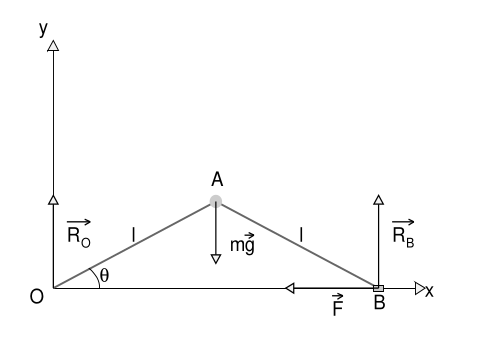
\includegraphics[width=0.7\textwidth]{images/mecanique_analytique/ma-001-000.png}
\caption{Système de treillis articulé : schéma.}
\end{figure}

\begin{figure}[H]
\centering

\includegraphics[width=0.7\textwidth]{images/mecanique_analytique/ma-001-001.png}
\caption{Forces et contraintes sur le treillis.}
\end{figure}

\begin{figure}[H]
\centering
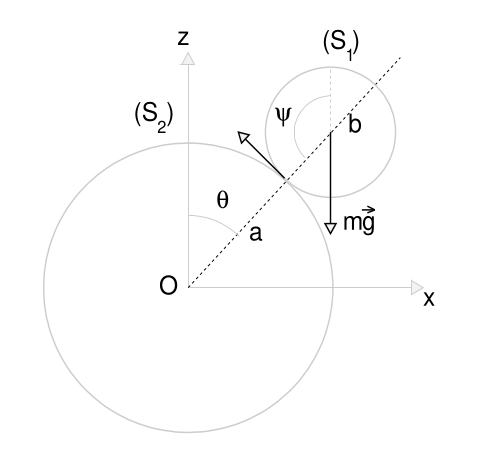
\includegraphics[width=0.7\textwidth]{images/mecanique_analytique/ma-003-002.png}
\caption{Roulement d'une sphère sur une autre.}
\end{figure}

\begin{figure}[H]
\centering

\includegraphics[width=0.7\textwidth]{images/mecanique_analytique/ma-003-003.png}
\caption{Électron en orbite : modèle planétaire.}
\end{figure}

\begin{figure}[H]
\centering
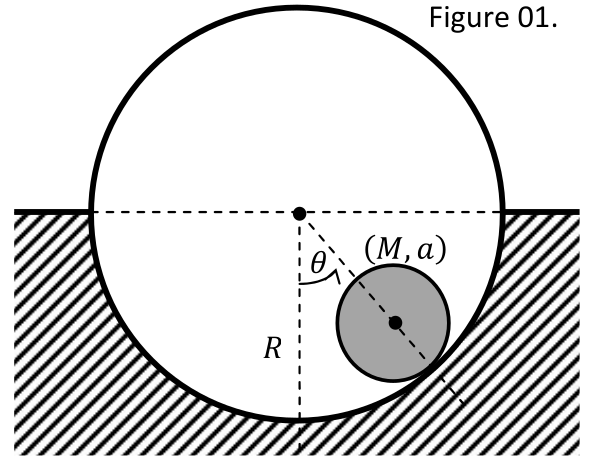
\includegraphics[width=0.7\textwidth]{images/mecanique_analytique/ma-011-004.png}
\caption{Pendule double : configuration.}
\end{figure}

\begin{figure}[H]
\centering

\includegraphics[width=0.7\textwidth]{images/mecanique_analytique/ma-011-005.png}
\caption{Modes normaux du pendule double.}
\end{figure}

\ifdefined\inMainDoc\else\end{document}\fi


% ================================================================
%  UE 8 : MÉCANIQUE DES MILIEUX CONTINUS
% ================================================================
\newpage
\thispagestyle{empty}
\begin{tikzpicture}[remember picture, overlay]
  \fill[gray!12] ([xshift=1.5cm, yshift=3cm]current page.south west)
    rectangle ([xshift=-1.5cm, yshift=-3cm]current page.north east);
  \draw[line width=3pt] ([xshift=1.5cm,yshift=-3cm]current page.north west)
    -- ([xshift=-1.5cm,yshift=-3cm]current page.north east);
  \draw[line width=3pt] ([xshift=1.5cm,yshift=3cm]current page.south west)
    -- ([xshift=-1.5cm,yshift=3cm]current page.south east);
  \node[align=center] at (current page.center) {%
    {\fontsize{24}{32}\bfseries\selectfont MÉCANIQUE DES MILIEUX}\\[0.3cm]
    {\fontsize{24}{32}\bfseries\selectfont CONTINUS}\\[1.0cm]
    {\large\itshape Tenseurs - Cinématique}\\[0.4cm]
    {\large\itshape Déformation - Contraintes}\\[1.5cm]
    {\normalsize Licence 3 - UE 8}
  };
  \node[anchor=south west] at ([xshift=2cm,yshift=2cm]current page.south west)
    {\large\bfseries UE 8};
\end{tikzpicture}
\newpage

\addcontentsline{toc}{section}{MÉCANIQUE DES MILIEUX CONTINUS}
\ifdefined\inMainDoc\else
\documentclass[12pt,a4paper]{article}
% ================================================================
%  PRÉAMBULE COMMUN - ANNALES CORRIGÉES
%  Université de Kara - FaST - Licence Fondamentale MPC
%  Design optimisé impression noir et blanc
% ================================================================

% -- ENCODAGE & LANGUE --
\usepackage[utf8]{inputenc}
\usepackage[T1]{fontenc}
\usepackage[french]{babel}
\usepackage{lmodern}
\usepackage{microtype}

% -- MISE EN PAGE --
\usepackage[a4paper, top=2.8cm, bottom=2.5cm, left=2.5cm, right=2.5cm, headheight=14pt]{geometry}
\usepackage{setspace}
\setstretch{1.2}
\usepackage{parskip}
\setlength{\parindent}{1.2em}
\setlength{\parskip}{4pt}

% -- MATHS --
\usepackage{amsmath, amssymb, mathtools, amsthm}
\usepackage{mathrsfs}
\usepackage{dsfont}
\usepackage{bm}
\usepackage{cancel}
\usepackage{textcomp}
% Définition de \oiint (intégrale de surface fermée) sans package supplémentaire
\newcommand{\oiint}{\mathop{\iint\!\!\!\!\!\!\!\bigcirc}\limits}

% -- PHYSIQUE & CHIMIE --
\usepackage{physics}
\usepackage{siunitx}
% Lorsque physics est chargé, siunitx omet \qty. On le restaure ici :
\AtBeginDocument{\RenewCommandCopy\qty\SI}
\sisetup{locale = FR, detect-all, output-decimal-marker={,}}
% Commande de substitution pour les unités posant problème avec pdflatex
% (ohm, degreeCelsius, micro, angstrom, percent utilisent des caractères non-ASCII)
\newcommand{\qtyohm}[1]{\ensuremath{\num{#1}\,\Omega}}
\newcommand{\qtydegc}[1]{\ensuremath{\num{#1}\,{}^\circ\text{C}}}
\newcommand{\qtyangstrom}[1]{\ensuremath{\num{#1}\,\text{\AA}}}
\newcommand{\qtypercent}[1]{\ensuremath{\num{#1}\,\%}}
\newcommand{\qtyum}[1]{\ensuremath{\num{#1}\,\mu\text{m}}}
\usepackage[version=4]{mhchem}

% -- GRAPHISMES --
\usepackage{graphicx}
\usepackage{float}
\usepackage{caption}
\usepackage{subcaption}
\usepackage{wrapfig}
\usepackage{tikz}
\usetikzlibrary{calc, arrows.meta, patterns, shapes.geometric}
\usepackage{pgfplots}
\pgfplotsset{compat=1.18}

% -- TABLEAUX --
\usepackage{booktabs}
\usepackage{array}
\usepackage{tabularx}
\usepackage{multirow}

% -- LISTES --
\usepackage{enumitem}
\setlist[enumerate]{topsep=3pt, itemsep=2pt, parsep=0pt}
\setlist[itemize]{topsep=3pt, itemsep=2pt, parsep=0pt, label={.}}

% -- BOÎTES (noir et blanc) --
\usepackage{mdframed}
\usepackage{tcolorbox}
\tcbuselibrary{skins, breakable, theorems}

% Boîte EXERCICE : encadré avec filet épais, fond blanc
\newmdenv[
  linewidth=1.2pt,
  linecolor=black,
  roundcorner=3pt,
  skipabove=10pt,
  skipbelow=6pt,
  innertopmargin=8pt,
  innerbottommargin=8pt,
  innerleftmargin=10pt,
  innerrightmargin=10pt,
  backgroundcolor=white,
  frametitle={\bfseries\small Exercice},
  frametitlealignment=\raggedright,
  frametitleaboveskip=4pt,
  frametitlebelowskip=4pt,
]{boiteexercice}

% Boîte CORRIGÉ : fond gris très clair + filet fin
\newmdenv[
  linewidth=0.6pt,
  linecolor=black,
  leftline=true,
  rightline=false,
  topline=false,
  bottomline=false,
  linecolor=black,
  innerleftmargin=12pt,
  innerrightmargin=8pt,
  innertopmargin=6pt,
  innerbottommargin=6pt,
  backgroundcolor=gray!8,
  skipabove=4pt,
  skipbelow=8pt,
]{boitecorrige}

% Boîte RÉSUMÉ DE COURS : double encadré
\newmdenv[
  linewidth=0.8pt,
  linecolor=black,
  roundcorner=2pt,
  backgroundcolor=gray!12,
  innertopmargin=10pt,
  innerbottommargin=10pt,
  innerleftmargin=12pt,
  innerrightmargin=12pt,
  skipabove=12pt,
  skipbelow=8pt,
]{boiteresume}

% Boîte ATTENTION/REMARQUE : barre gauche épaisse
\newmdenv[
  leftline=true,
  rightline=false,
  topline=false,
  bottomline=false,
  linewidth=3pt,
  linecolor=black,
  backgroundcolor=gray!5,
  innerleftmargin=12pt,
  innerrightmargin=8pt,
  innertopmargin=5pt,
  innerbottommargin=5pt,
  skipabove=6pt,
  skipbelow=6pt,
]{boiteremarque}

% -- DIFFICULTÉ DES EXERCICES --
\newcommand{\facile}{$\star$}
\newcommand{\moyen}{$\star\!\star$}
\newcommand{\difficile}{$\star\!\star\!\star$}
\newcommand{\niveau}[1]{\hfill\textbf{#1}\hspace{2pt}}

% -- EN-TÊTES ET PIEDS DE PAGE --
\usepackage{fancyhdr}
\pagestyle{fancy}
\fancyhf{}
\renewcommand{\headrulewidth}{0.5pt}
\renewcommand{\footrulewidth}{0.3pt}

% -- HYPERLIENS --
\usepackage[hidelinks]{hyperref}
\hypersetup{
    colorlinks=false,
    pdftitle={Annale Corrigée - Licence MPC - Université de Kara}
}

% -- TITRES --
\usepackage{titlesec}
\titleformat{\section}{\Large\bfseries}{\thesection.}{0.8em}{}[\vspace{2pt}\hrule\vspace{4pt}]
\titleformat{\subsection}{\large\bfseries}{\thesubsection.}{0.7em}{}
\titleformat{\subsubsection}{\normalsize\bfseries}{\thesubsubsection.}{0.6em}{}

% -- THÉORÈMES --
\theoremstyle{definition}
\newtheorem{defn}{Définition}[section]
\newtheorem{prop}{Propriété}[section]
\newtheorem{thm}{Théorème}[section]
\newtheorem{corol}{Corollaire}[section]
\newtheorem{exemple}{Exemple}[section]

% -- COMMANDES MATHÉMATIQUES UTILES --
\newcommand{\vect}[1]{\overrightarrow{#1}}
\newcommand{\R}{\mathbb{R}}
\newcommand{\N}{\mathbb{N}}
\newcommand{\Z}{\mathbb{Z}}
\newcommand{\C}{\mathbb{C}}
\renewcommand{\d}{\mathrm{d}}
\newcommand{\deriv}[2]{\dfrac{\d #1}{\d #2}}
\newcommand{\dpart}[2]{\dfrac{\partial #1}{\partial #2}}
\newcommand{\rot}{\overrightarrow{\mathrm{rot}}\,}
\renewcommand{\div}{\mathrm{div}\,}
\renewcommand{\grad}{\overrightarrow{\mathrm{grad}}\,}
\newcommand{\e}{\mathrm{e}}
\newcommand{\ii}{\mathrm{i}}
\renewcommand{\Tr}{\mathrm{Tr}}

% Numérotation des équations par section
\numberwithin{equation}{section}

% -- RÉSULTATS ENCADRÉS --
\newcommand{\res}[1]{\[\boxed{#1}\]}

% -- REMARQUE INLINE --
\newcommand{\rmq}[1]{\begin{boiteremarque}\textbf{Remarque.} #1\end{boiteremarque}}

% -- MISE EN VALEUR DU RÉSULTAT FINAL --
\newcommand{\reponse}[1]{%
  \begin{center}
    \fbox{\begin{minipage}{0.92\textwidth}\centering #1\end{minipage}}
  \end{center}%
}


\lhead{\small\textit{Mécanique des Milieux Continus - Licence 3}}
\rhead{\small\textit{FaST, Université de Kara}}
\cfoot{\thepage}

\begin{document}
\fi

\begin{center}
  {\LARGE\bfseries MÉCANIQUE DES MILIEUX CONTINUS}\\[0.3cm]
  {\normalsize Licence 3 - Physique}\\[0.1cm]
  \rule{0.7\textwidth}{0.8pt}
\end{center}

\section*{Résumé du cours}

\begin{boiteresume}

\textbf{1. Algèbre tensorielle.} Un tenseur d'ordre 2 $\overline{\overline{T}}$ a des composantes $T_{ij}$ dans une base orthonormée. La règle de changement de base : $T'_{ij} = \alpha_{ip}\alpha_{jq}T_{pq}$ (convention d'Einstein). Symétrie ($T_{ij}=T_{ji}$) et antisymétrie ($T_{ij}=-T_{ji}$) sont des propriétés tensorielles. Tout tenseur se décompose : $\overline{\overline{T}} = \overline{\overline{T}}^S + \overline{\overline{T}}^A$ avec $\overline{\overline{T}}^S = \frac{1}{2}(\overline{\overline{T}}+\overline{\overline{T}}^T)$ et $\overline{\overline{T}}^A = \frac{1}{2}(\overline{\overline{T}}-\overline{\overline{T}}^T)$. Produit doublement contracté : $\overline{\overline{S}}:\overline{\overline{T}} = S_{ij}T_{ji}$.

\textbf{2. Cinématique des milieux continus.} Description lagrangienne : $\vec{x} = \vec{\chi}(\vec{X}, t)$ où $\vec{X}$ est la position initiale. Tenseur gradient de la transformation : $F_{iJ} = \partial x_i/\partial X_J$. Tenseur des dilatations de Cauchy-Green à droite : $\overline{\overline{C}} = \overline{\overline{F}}^T\overline{\overline{F}}$. Tenseur des déformations de Green-Lagrange : $\overline{\overline{E}} = \frac{1}{2}(\overline{\overline{C}}-\overline{\overline{I}})$. Jacobien : $J = \det\overline{\overline{F}} > 0$ (conservation de la masse : $\rho J = \rho_0$).

\textbf{3. Cinématique eulérienne.} Tenseur gradient de vitesse : $\overline{\overline{L}} = \overline{\mathrm{grad}}\,\vec{V}$. Décomposition : $\overline{\overline{L}} = \overline{\overline{D}} + \overline{\overline{\Omega}}$ où $\overline{\overline{D}} = \frac{1}{2}(\overline{\overline{L}}+\overline{\overline{L}}^T)$ est le tenseur des taux de déformation et $\overline{\overline{\Omega}} = \frac{1}{2}(\overline{\overline{L}}-\overline{\overline{L}}^T)$ le tenseur des taux de rotation. Conservation de la masse : $\frac{\partial \rho}{\partial t} + \mathrm{div}(\rho\vec{V}) = 0$.

\textbf{4. Mouvement rigidifiant.} Un mouvement est rigidifiant si et seulement si $\overline{\overline{E}} = \overline{\overline{0}}$ (ou de manière équivalente $\overline{\overline{D}} = \overline{\overline{0}}$). Le tenseur des dilatations vaut alors $\overline{\overline{C}} = \overline{\overline{I}}$ : aucune déformation, seul une rotation globale du solide.

\textbf{5. Équations du mouvement.} Équation d'équilibre (quasi-statique) : $\mathrm{div}\,\overline{\overline{\sigma}} + \rho\vec{f} = \vec{0}$. Loi de comportement élastique linéaire (isotrope) : $\overline{\overline{\sigma}} = \lambda(\mathrm{tr}\,\overline{\overline{\varepsilon}})\overline{\overline{I}} + 2\mu\overline{\overline{\varepsilon}}$ avec $\overline{\overline{\varepsilon}}$ le tenseur des petites déformations.

\end{boiteresume}

\newpage
\section{Algèbre tensorielle}

\subsection*{Exercice 1 - Propriétés tensorielles de la symétrie \niveau{\facile}}

\begin{boiteexercice}
Soit $\overline{\overline{S}}$ un tenseur d'ordre 2 symétrique ($S_{ij}=S_{ji}$) dans une base orthonormée $B$. Montrer que cette propriété de symétrie est conservée dans toute autre base orthonormée $B'$.
\end{boiteexercice}

\begin{boitecorrige}
Soit $\alpha_{ij}$ la matrice de passage de $B$ à $B'$. Dans la base $B'$, les composantes de $\overline{\overline{S}}$ sont données par la loi de changement de base :
\[
S'_{ij} = \alpha_{ip}\,\alpha_{jq}\,S_{pq}
\]
On veut montrer que $S'_{ij} = S'_{ji}$. Puisque $S_{pq} = S_{qp}$, on peut intervertir les indices muets $p \leftrightarrow q$ :
\[
S'_{ij} = \alpha_{ip}\,\alpha_{jq}\,S_{pq} = \alpha_{ip}\,\alpha_{jq}\,S_{qp} = \alpha_{jq}\,\alpha_{ip}\,S_{qp}
\]
Or, en renommant les indices muets ($p \to q$, $q \to p$) dans l'expression de $S'_{ji}$ :
\[
S'_{ji} = \alpha_{jp}\,\alpha_{iq}\,S_{pq}
\]
En intervertissant $p \leftrightarrow q$ dans $S'_{ij}$ : $S'_{ij} = \alpha_{jp}\,\alpha_{iq}\,S_{pq} = S'_{ji}$. La symétrie est bien une propriété tensorielle.
\end{boitecorrige}

\subsection*{Exercice 2 - Décomposition d'un tenseur \niveau{\facile}}

\begin{boiteexercice}
\begin{enumerate}
  \item Montrer que tout tenseur $\overline{\overline{T}}$ peut se décomposer en une partie symétrique $\overline{\overline{T}}^S$ et une partie antisymétrique $\overline{\overline{T}}^A$.
  \item Montrer que pour $\overline{\overline{S}}$ symétrique et $\overline{\overline{A}}$ antisymétrique, on a $\overline{\overline{S}}:\overline{\overline{A}} = 0$.
  \item En déduire que $\overline{\overline{S}}:\overline{\overline{T}} = \overline{\overline{S}}:\overline{\overline{T}}^S$.
\end{enumerate}
\end{boiteexercice}

\begin{boitecorrige}
\textbf{1.} On pose :
\[
\overline{\overline{T}}^S = \frac{1}{2}(\overline{\overline{T}}+\overline{\overline{T}}^T), \qquad \overline{\overline{T}}^A = \frac{1}{2}(\overline{\overline{T}}-\overline{\overline{T}}^T)
\]
En composantes : $T^S_{ij} = \frac{1}{2}(T_{ij}+T_{ji}) = T^S_{ji}$ (symétrique) et $T^A_{ij} = \frac{1}{2}(T_{ij}-T_{ji}) = -T^A_{ji}$ (antisymétrique). On vérifie $\overline{\overline{T}}^S + \overline{\overline{T}}^A = \overline{\overline{T}}$.

\textbf{2.} En développant explicitement $\overline{\overline{S}}:\overline{\overline{A}} = S_{ij}A_{ji}$ :
\[
\overline{\overline{S}}:\overline{\overline{A}} = \sum_{i,j} S_{ij}A_{ji}
\]
Les termes diagonaux sont nuls ($A_{ii}=0$ car antisymétrique). Pour les termes hors diagonale, par symétrie $S_{ij}=S_{ji}$ et antisymétrie $A_{ij}=-A_{ji}$ :
\[
S_{12}A_{21} + S_{21}A_{12} = S_{12}A_{21} + S_{12}(-A_{21}) = 0
\]
et de même pour les autres paires. Donc $\overline{\overline{S}}:\overline{\overline{A}} = 0$.

\textbf{3.} Par distributivité et le résultat précédent :
\[
\overline{\overline{S}}:\overline{\overline{T}} = \overline{\overline{S}}:(\overline{\overline{T}}^S + \overline{\overline{T}}^A) = \overline{\overline{S}}:\overline{\overline{T}}^S + \underbrace{\overline{\overline{S}}:\overline{\overline{T}}^A}_{=0} = \overline{\overline{S}}:\overline{\overline{T}}^S
\]
\end{boitecorrige}

\section{Cinématique des milieux continus}

\subsection*{Exercice 3 - Rotation solide \niveau{\moyen}}

\begin{boiteexercice}
On considère le mouvement défini en représentation lagrangienne par ($\omega$ constante positive) :
\[
\begin{cases}
x_1 = X_1\cos(\omega t) - X_2\sin(\omega t)\\
x_2 = X_1\sin(\omega t) + X_2\cos(\omega t)\\
x_3 = X_3
\end{cases}
\]
\begin{enumerate}
  \item Calculer le tenseur gradient $\overline{\overline{F}}$, le tenseur des dilatations $\overline{\overline{C}}$ et le tenseur des déformations $\overline{\overline{E}}$.
  \item À quelle classe particulière ce mouvement appartient-il ? Justifier.
  \item Calculer le jacobien $J$ et en déduire la masse volumique à l'instant $t$.
  \item Calculer les champs de vitesse et d'accélération lagrangiens.
  \item Exprimer $\vec{V}$ et $\vec{\gamma}$ en coordonnées eulériennes. Calculer $\overline{\overline{D}}$ et $\overline{\overline{\Omega}}$.
\end{enumerate}
\end{boiteexercice}

\begin{boitecorrige}
\textbf{1.} Le terme général de $\overline{\overline{F}}$ est $F_{iJ} = \partial x_i/\partial X_J$ :
\[
\overline{\overline{F}} = \begin{pmatrix}\cos\omega t & -\sin\omega t & 0\\ \sin\omega t & \cos\omega t & 0\\ 0 & 0 & 1\end{pmatrix}
\]
Tenseur des dilatations $\overline{\overline{C}} = \overline{\overline{F}}^T\overline{\overline{F}}$ :
\[
\overline{\overline{C}} = \begin{pmatrix}\cos\omega t & \sin\omega t & 0\\ -\sin\omega t & \cos\omega t & 0\\ 0 & 0 & 1\end{pmatrix}\begin{pmatrix}\cos\omega t & -\sin\omega t & 0\\ \sin\omega t & \cos\omega t & 0\\ 0 & 0 & 1\end{pmatrix} = \begin{pmatrix}1&0&0\\0&1&0\\0&0&1\end{pmatrix} = \overline{\overline{I}}
\]
Donc $\overline{\overline{E}} = \frac{1}{2}(\overline{\overline{C}}-\overline{\overline{I}}) = \overline{\overline{0}}$.

\textbf{2.} Puisque $\overline{\overline{E}} = \overline{\overline{0}}$, ce mouvement est \textbf{rigidifiant} : c'est une rotation pure autour de l'axe $\vec{e}_3$ à vitesse angulaire $\omega$.

\textbf{3.} $J = \det\overline{\overline{F}} = \cos^2\omega t + \sin^2\omega t = 1$. La conservation de la masse $\rho J = \rho_0$ donne $\rho = \rho_0$ : la masse volumique est constante.

\textbf{4.} Le champ de vitesse lagrangien $\vec{V} = D\vec{x}/Dt$ :
\[
\begin{cases}
V_1 = -\omega X_1\sin\omega t - \omega X_2\cos\omega t\\
V_2 = \omega X_1\cos\omega t - \omega X_2\sin\omega t\\
V_3 = 0
\end{cases}
\]
L'accélération $\vec{\gamma} = D\vec{V}/Dt$ :
\[
\begin{cases}
\gamma_1 = -\omega^2(X_1\cos\omega t - X_2\sin\omega t) = -\omega^2 x_1\\
\gamma_2 = -\omega^2(X_1\sin\omega t + X_2\cos\omega t) = -\omega^2 x_2\\
\gamma_3 = 0
\end{cases}
\]

\textbf{5.} En inversant la transformation ($X_1 = x_1\cos\omega t + x_2\sin\omega t$, $X_2 = -x_1\sin\omega t + x_2\cos\omega t$), on exprime $\vec{V}$ en coordonnées eulériennes :
\[
\vec{V}(\vec{x},t) = \omega(-x_2\vec{e}_1 + x_1\vec{e}_2)
\]
Le tenseur gradient de vitesse $\overline{\overline{L}} = \overline{\mathrm{grad}}\,\vec{V}$ a pour composantes $L_{ij} = \partial V_i/\partial x_j$ :
\[
\overline{\overline{L}} = \omega\begin{pmatrix}0&-1&0\\1&0&0\\0&0&0\end{pmatrix}
\]
$\overline{\overline{L}}$ est antisymétrique, donc $\overline{\overline{D}} = \overline{\overline{0}}$ et $\overline{\overline{\Omega}} = \overline{\overline{L}}$. Le taux de rotation est $\omega$ autour de $\vec{e}_3$.
\end{boitecorrige}

\subsection*{Exercice 4 - Cinématique d'un tourbillon \niveau{\moyen}}

\begin{boiteexercice}
On considère un mouvement eulérien défini par :
\[
\vec{V}(x_1,x_2) = A(x_1,x_2)\begin{pmatrix}-x_2\\x_1\\0\end{pmatrix}, \quad A = \frac{\alpha}{2\pi(x_1^2+x_2^2)}
\]
où $\alpha$ est une constante positive, défini pour $x_1^2+x_2^2 > 0$.
\begin{enumerate}
  \item De quel type de mouvement s'agit-il qualitativement ?
  \item Calculer la matrice du tenseur gradient de vitesse $\overline{\overline{L}}$.
  \item En déduire $\overline{\overline{D}}$ et $\overline{\overline{\Omega}}$. Commenter.
  \item Calculer $\mathrm{div}\,\vec{V}$ et en déduire la masse volumique à tout instant.
\end{enumerate}
\end{boiteexercice}

\begin{boitecorrige}
\textbf{1.} Les lignes de courant sont des cercles centrés à l'origine. Il s'agit d'un \textbf{tourbillon} (ou vortex) à circulation constante.

\textbf{2.} Avec $A = \alpha/[2\pi(x_1^2+x_2^2)]$, les dérivées partielles de $V_1 = -Ax_2$ et $V_2 = Ax_1$ donnent :
\[
\overline{\overline{L}} = \frac{A}{x_1^2+x_2^2}\begin{pmatrix}2x_1x_2 & x_2^2-x_1^2 & 0\\ x_2^2-x_1^2 & -2x_1x_2 & 0\\ 0 & 0 & 0\end{pmatrix}
\]

\textbf{3.} La partie symétrique $\overline{\overline{D}} = \frac{1}{2}(\overline{\overline{L}}+\overline{\overline{L}}^T)$ et la partie antisymétrique $\overline{\overline{\Omega}} = \frac{1}{2}(\overline{\overline{L}}-\overline{\overline{L}}^T)$ :

On vérifie que $\overline{\overline{L}}$ est \textbf{symétrique} (puisque $L_{12}=L_{21}$ et $L_{11}+L_{22}=0$). Donc $\overline{\overline{D}} = \overline{\overline{L}}$ et $\overline{\overline{\Omega}} = \overline{\overline{0}}$. Le mouvement a des taux de déformation non nuls mais aucune rotation instantanée : paradoxalement, ce tourbillon est \textit{irrotationnel}.

\textbf{4.} $\mathrm{div}\,\vec{V} = \partial V_1/\partial x_1 + \partial V_2/\partial x_2 = \frac{2Ax_1x_2}{x_1^2+x_2^2} + \frac{-2Ax_1x_2}{x_1^2+x_2^2} = 0$.

L'écoulement est incompressible : $\frac{D\rho}{Dt} = -\rho\,\mathrm{div}\,\vec{V} = 0$, donc $\rho = \rho_0$ (constante en tout point et tout instant).
\end{boitecorrige}

\subsection*{Exercice 5 - Petites déformations \niveau{\difficile}}

\begin{boiteexercice}
Un milieu élastique linéaire isotrope (module de Young $E=\qty{210}{GPa}$, coefficient de Poisson $\nu=0{,}3$) est soumis à un état de contrainte uniaxial : $\sigma_{11} = \sigma_0$, toutes les autres composantes nulles.
\begin{enumerate}
  \item Rappeler la loi de comportement de Hooke généralisée reliant $\overline{\overline{\varepsilon}}$ à $\overline{\overline{\sigma}}$.
  \item Calculer toutes les composantes du tenseur des petites déformations $\varepsilon_{ij}$.
  \item Calculer la dilatation volumique $\theta = \mathrm{tr}\,\overline{\overline{\varepsilon}}$.
  \item Calculer les coefficients de Lamé $\lambda$ et $\mu$ (module de cisaillement) en fonction de $E$ et $\nu$.
\end{enumerate}
\end{boiteexercice}

\begin{boitecorrige}
\textbf{1.} Loi de Hooke généralisée (isotrope) :
\[
\varepsilon_{ij} = \frac{1+\nu}{E}\sigma_{ij} - \frac{\nu}{E}(\mathrm{tr}\,\overline{\overline{\sigma}})\delta_{ij}
\]

\textbf{2.} Ici $\mathrm{tr}\,\overline{\overline{\sigma}} = \sigma_0$. On obtient :
\[
\varepsilon_{11} = \frac{1+\nu}{E}\sigma_0 - \frac{\nu}{E}\sigma_0 = \frac{\sigma_0}{E}
\]
\[
\varepsilon_{22} = \varepsilon_{33} = 0 - \frac{\nu}{E}\sigma_0 = -\frac{\nu\sigma_0}{E}
\]
Toutes les composantes de cisaillement ($i\neq j$) sont nulles.

Application numérique : $\varepsilon_{11} = \sigma_0/210\,\text{GPa}$, $\varepsilon_{22}=\varepsilon_{33}=-0{,}3\sigma_0/210\,\text{GPa}$.

\textbf{3.} Dilatation volumique :
\[
\theta = \varepsilon_{11}+\varepsilon_{22}+\varepsilon_{33} = \frac{\sigma_0}{E} - \frac{2\nu\sigma_0}{E} = \frac{(1-2\nu)\sigma_0}{E} = \frac{0{,}4\,\sigma_0}{210\,\text{GPa}}
\]

\textbf{4.} Les coefficients de Lamé :
\[
\mu = \frac{E}{2(1+\nu)} = \frac{210}{2\times1{,}3} \approx \qty{80.8}{GPa}
\]
\[
\lambda = \frac{E\nu}{(1+\nu)(1-2\nu)} = \frac{210\times0{,}3}{1{,}3\times0{,}4} \approx \qty{121}{GPa}
\]
\end{boitecorrige}


\section{Cinématique avancée}

\subsection*{Exercice 6 - Rotation solide en coordonnées polaires \niveau{\difficile}}

\begin{boiteexercice}
On considère le mouvement défini en représentation lagrangienne par ($\omega$ constante positive) :
\[
\begin{cases}
x_1 = X_1\cos(\omega t) - X_2\sin(\omega t)\\
x_2 = X_1\sin(\omega t) + X_2\cos(\omega t)\\
x_3 = X_3
\end{cases}
\]
\begin{enumerate}
  \item Calculer $\overline{\overline{F}}$, $\overline{\overline{C}}$, $\overline{\overline{E}}$. À quelle classe ce mouvement appartient-il ?
  \item Calculer le jacobien $J$ et en déduire la masse volumique.
  \item Calculer les champs de vitesse et d'accélération lagrangiens, puis eulériens. En déduire $\overline{\overline{D}}$ et $\overline{\overline{\Omega}}$.
  \item En coordonnées polaires lagrangiennes $(R,\Theta)$ et eulériennes $(r,\theta)$, exprimer les fonctions $X_r$ et $X_\theta$ définissant le mouvement.
  \item Exprimer le champ de vitesse en coordonnées polaires dans la base $B' = (\vec{e}_r, \vec{e}_\theta, \vec{e}_3)$.
  \item Calculer l'accélération centripète $\gamma_r$ et tangentielle $\gamma_\theta$.
  \item Définir les trajectoires du mouvement.
\end{enumerate}
\end{boiteexercice}

\begin{boitecorrige}
\textbf{1.} $\overline{\overline{F}} = \begin{pmatrix}\cos\omega t & -\sin\omega t & 0\\ \sin\omega t & \cos\omega t & 0\\ 0 & 0 & 1\end{pmatrix}$, $\overline{\overline{C}} = \overline{\overline{F}}^T\overline{\overline{F}} = \overline{\overline{I}}$, donc $\overline{\overline{E}} = \overline{\overline{0}}$ : \textbf{mouvement rigidifiant} (rotation pure).

\textbf{2.} $J = \det\overline{\overline{F}} = \cos^2\omega t + \sin^2\omega t = 1$, donc $\rho = \rho_0$ (masse volumique constante).

\textbf{3.} Champ de vitesse lagrangien $\vec{V} = D\vec{x}/Dt$ :
\[
V_1 = -\omega X_1\sin\omega t - \omega X_2\cos\omega t, \quad V_2 = \omega X_1\cos\omega t - \omega X_2\sin\omega t, \quad V_3 = 0
\]
Accélération lagrangienne : $\gamma_1 = -\omega^2 x_1$, $\gamma_2 = -\omega^2 x_2$, $\gamma_3 = 0$.

En coordonnées eulériennes (en inversant la transformation) :
\[
\vec{V}(\vec{x},t) = \omega(-x_2\vec{e}_1 + x_1\vec{e}_2), \qquad \vec{\gamma} = -\omega^2(x_1\vec{e}_1 + x_2\vec{e}_2)
\]
Le tenseur $\overline{\overline{L}} = \overline{\mathrm{grad}}\,\vec{V}$ est antisymétrique : $\overline{\overline{D}} = \overline{\overline{0}}$ et $\overline{\overline{\Omega}} = \overline{\overline{L}} = \omega\begin{pmatrix}0&-1&0\\1&0&0\\0&0&0\end{pmatrix}$.

\textbf{4.} En passant aux coordonnées polaires : $r = \sqrt{x_1^2+x_2^2} = R$ et $\theta = \Theta + \omega t$.
\[
\begin{cases} r = R \\ \theta = \Theta + \omega t \end{cases}
\]

\textbf{5.} En remplaçant $x_1 = r\cos\theta$, $x_2 = r\sin\theta$ dans $\vec{V} = \omega(-x_2\vec{e}_1 + x_1\vec{e}_2)$, et en utilisant $\vec{e}_\theta = -\sin\theta\,\vec{e}_1 + \cos\theta\,\vec{e}_2$ :
\[
\vec{V} = \omega r\,\vec{e}_\theta \quad\Longrightarrow\quad V_r = 0,\; V_\theta = \omega r,\; V_3 = 0
\]

\textbf{6.} En polaires, $\vec{\gamma} = -\omega^2 r\,\vec{e}_r$ : accélération purement \textbf{centripète}.
\[
\gamma_r = -\omega^2 r, \qquad \gamma_\theta = 0
\]

\textbf{7.} Les trajectoires sont des \textbf{cercles centrés à l'origine}, de rayon $R$ constant, parcourus à vitesse angulaire $\omega$ (constante).
\end{boitecorrige}

\subsection*{Exercice 7 - Étude d'un tourbillon (examen partiel) \niveau{\difficile}}

\begin{boiteexercice}
On considère un mouvement eulérien défini par :
\[
\begin{cases}
V_1 = -A(x_1,x_2)\,x_2\\
V_2 = A(x_1,x_2)\,x_1\\
V_3 = 0
\end{cases}
\quad\text{avec}\quad A(x_1,x_2) = \frac{\alpha}{2\pi(x_1^2+x_2^2)},\; \alpha > 0
\]
défini pour $x_1^2 + x_2^2 > 0$.
\begin{enumerate}
  \item De quel type de mouvement s'agit-il ?
  \item Montrer que la matrice du tenseur gradient de vitesse $\overline{\overline{L}}$ est :
  \[
  \overline{\overline{L}} = \frac{A}{x_1^2+x_2^2}\begin{bmatrix}2x_1x_2 & x_2^2-x_1^2 & 0\\ x_2^2-x_1^2 & -2x_1x_2 & 0\\ 0 & 0 & 0\end{bmatrix}_B
  \]
  \item En déduire $\overline{\overline{\Omega}}$ et $\overline{\overline{D}}$. Commenter.
  \item Calculer $\mathrm{div}\,\vec{V}$ et en déduire la masse volumique.
\end{enumerate}
\end{boiteexercice}

\begin{boitecorrige}
\textbf{1.} Le mouvement est \textbf{plan, permanent et isochore} (tourbillon irrotationnel).

\textbf{2.} On calcule $\partial A/\partial x_i$ puis les dérivées $L_{ij} = \partial V_i/\partial x_j$ :
\[
\frac{\partial A}{\partial x_1} = -A\frac{2x_1}{x_1^2+x_2^2}, \quad \frac{\partial A}{\partial x_2} = -A\frac{2x_2}{x_1^2+x_2^2}
\]
On obtient :
\begin{align*}
L_{11} = \frac{\partial V_1}{\partial x_1} &= \frac{2Ax_1x_2}{x_1^2+x_2^2}, \quad
L_{12} = \frac{\partial V_1}{\partial x_2} = \frac{A(x_2^2-x_1^2)}{x_1^2+x_2^2}\\
L_{21} = \frac{\partial V_2}{\partial x_1} &= \frac{A(x_2^2-x_1^2)}{x_1^2+x_2^2}, \quad
L_{22} = \frac{\partial V_2}{\partial x_2} = \frac{-2Ax_1x_2}{x_1^2+x_2^2}
\end{align*}
La matrice obtenue est bien celle de l'énoncé.

\textbf{3.} La matrice $\overline{\overline{L}}$ est \textbf{symétrique} ($L_{12} = L_{21}$). Donc $\overline{\overline{\Omega}} = \overline{\overline{0}}$ et $\overline{\overline{D}} = \overline{\overline{L}}$. \textit{Paradoxalement, ce tourbillon est irrotationnel} (pas de rotation instantanée) mais présente des taux de déformation non nuls.

\textbf{4.} $\mathrm{div}\,\vec{V} = L_{11} + L_{22} + L_{33} = \frac{2Ax_1x_2 - 2Ax_1x_2}{x_1^2+x_2^2} + 0 = 0$.

Le mouvement est incompressible, donc $D\rho/Dt = 0$ et $\rho = \rho_0$ en tout point et tout instant.
\end{boitecorrige}


\newpage
\section{Mécanique des milieux continus : contraintes et déformations}

\subsection*{Exercice 8 - Tenseur des contraintes : définition et équilibre \niveau{\moyen}}

\begin{boiteexercice}
Le tenseur des contraintes de Cauchy $\overline{\overline{\sigma}}$ est défini par $\vec{t} = \overline{\overline{\sigma}}\cdot\hat{n}$ où $\vec{t}$ est le vecteur contrainte sur la facette de normale $\hat{n}$.
\begin{enumerate}
  \item Définir les composantes normales ($\sigma_{ii}$) et tangentielles ($\sigma_{ij}$, $i\neq j$) du tenseur.
  \item Montrer par un raisonnement sur un tétraèdre de Cauchy que $\overline{\overline{\sigma}}$ est bien un tenseur du second ordre.
  \item En appliquant le bilan des forces sur un volume élémentaire, établir les équations d'équilibre statique :
  \[
  \frac{\partial\sigma_{ij}}{\partial x_j} + f_i = 0
  \]
  où $f_i$ est la composante $i$ de la force volumique.
  \item Montrer par un bilan du moment cinétique que $\overline{\overline{\sigma}}$ est symétrique : $\sigma_{ij} = \sigma_{ji}$.
\end{enumerate}
\end{boiteexercice}

\begin{boitecorrige}
\textbf{1.} Le tenseur des contraintes $\overline{\overline{\sigma}}$ est la matrice $3\times3$ dont l'élément $\sigma_{ij}$ représente la force par unité de surface dans la direction $\vec{e}_i$ exercée sur la facette de normale $\vec{e}_j$.
\begin{itemize}
  \item Composantes \textbf{normales} ($i=j$) : $\sigma_{11},\sigma_{22},\sigma_{33}$ ; contraintes de traction ($>0$) ou compression ($<0$).
  \item Composantes \textbf{tangentielles} ($i\neq j$) : $\sigma_{12},\sigma_{13},\ldots$ ; contraintes de cisaillement.
\end{itemize}

\textbf{2.} On considère un tétraèdre de Cauchy de faces de normales $\hat{n}$ et $-\vec{e}_1$, $-\vec{e}_2$, $-\vec{e}_3$. Le bilan de forces à l'équilibre (en négligeant les forces volumiques d'ordre 3 devant les forces de surface d'ordre 2) donne :
\[
t_i(\hat{n}) = \sigma_{ij}n_j
\]
ce qui montre que le vecteur contrainte $\vec{t}$ est l'image linéaire de $\hat{n}$ par $\overline{\overline{\sigma}}$ : c'est bien un tenseur.

\textbf{3.} Sur un volume élémentaire $dV$, la force de surface est $\oint_{\partial V}\sigma_{ij}n_j\,\d S$. Par le théorème de la divergence et en appliquant la deuxième loi de Newton (équilibre statique $\rho\vec{a}=\vec{0}$) :
\[
\int_V\left(\frac{\partial\sigma_{ij}}{\partial x_j} + f_i\right)\d V = 0
\]
Pour tout volume $V$, cela implique $\dfrac{\partial\sigma_{ij}}{\partial x_j} + f_i = 0$.

\textbf{4.} Le bilan du moment cinétique sur un volume élémentaire, en ne retenant que les termes dominants (d'ordre surface$^2$), donne $\sigma_{ij}-\sigma_{ji}=0$ pour tout $i,j$ : le tenseur des contraintes est symétrique.
\end{boitecorrige}

\subsection*{Exercice 9 - Tenseur des petites déformations \niveau{\moyen}}

\begin{boiteexercice}
Pour un déplacement $\vec{u}(\vec{x})$ petits (approximation linéaire), le tenseur des petites déformations est :
\[
\varepsilon_{ij} = \frac{1}{2}\left(\frac{\partial u_i}{\partial x_j} + \frac{\partial u_j}{\partial x_i}\right)
\]
\begin{enumerate}
  \item Interpréter physiquement les composantes diagonales $\varepsilon_{ii}$ et les composantes de cisaillement $\varepsilon_{ij}$ ($i\neq j$).
  \item Calculer la déformation volumique $\theta = \varepsilon_{kk} = \text{tr}\,\overline{\overline{\varepsilon}} = \text{div}\,\vec{u}$.
  \item Pour le champ de déplacement $\vec{u} = (ax_1, bx_2, cx_3)$ ($a,b,c$ constants), calculer $\overline{\overline{\varepsilon}}$ et $\theta$.
  \item Pour $\vec{u} = \alpha(-x_2, x_1, 0)$ ($\alpha$ petit), calculer $\overline{\overline{\varepsilon}}$. Quel type de déformation s'agit-il ?
  \item Décomposer un déplacement quelconque en une partie déformation pure et une partie rotation.
\end{enumerate}
\end{boiteexercice}

\begin{boitecorrige}
\textbf{1.}
\begin{itemize}
  \item $\varepsilon_{11} = \partial u_1/\partial x_1$ : allongement relatif dans la direction $\vec{e}_1$.
  \item $\varepsilon_{12} = \frac{1}{2}(\partial u_1/\partial x_2 + \partial u_2/\partial x_1)$ : demi-angle de glissement entre les directions $\vec{e}_1$ et $\vec{e}_2$.
\end{itemize}

\textbf{2.} La déformation volumique :
\[
\theta = \varepsilon_{11}+\varepsilon_{22}+\varepsilon_{33} = \frac{\partial u_1}{\partial x_1}+\frac{\partial u_2}{\partial x_2}+\frac{\partial u_3}{\partial x_3} = \text{div}\,\vec{u}
\]

\textbf{3.} Pour $\vec{u} = (ax_1, bx_2, cx_3)$ :
\[
\overline{\overline{\varepsilon}} = \begin{pmatrix}a&0&0\\0&b&0\\0&0&c\end{pmatrix}, \qquad\theta = a+b+c
\]
Déformation homogène sans cisaillement.

\textbf{4.} Pour $\vec{u} = \alpha(-x_2, x_1, 0)$ :
\[
\frac{\partial u_1}{\partial x_1}=0,\quad\frac{\partial u_1}{\partial x_2}=-\alpha,\quad\frac{\partial u_2}{\partial x_1}=\alpha,\quad\frac{\partial u_2}{\partial x_2}=0
\]
\[
\varepsilon_{12} = \frac{1}{2}(-\alpha+\alpha) = 0
\]
Donc $\overline{\overline{\varepsilon}} = \overline{\overline{0}}$ : c'est une \textbf{rotation pure} de petite amplitude $\alpha$ autour de $\vec{e}_3$. Il n'y a aucune déformation.

\textbf{5.} Le gradient de déplacement se décompose en :
\[
\frac{\partial u_i}{\partial x_j} = \varepsilon_{ij} + \omega_{ij}, \quad\omega_{ij} = \frac{1}{2}\left(\frac{\partial u_i}{\partial x_j}-\frac{\partial u_j}{\partial x_i}\right)
\]
$\overline{\overline{\varepsilon}}$ est symétrique (déformation pure) et $\overline{\overline{\omega}}$ est antisymétrique (rotation infinitésimale).
\end{boitecorrige}

\subsection*{Exercice 10 - Loi de Hooke généralisée et coefficients de Lamé \niveau{\moyen}}

\begin{boiteexercice}
Pour un milieu élastique linéaire isotrope, la loi de Hooke généralisée s'écrit :
\[
\sigma_{ij} = \lambda\varepsilon_{kk}\delta_{ij} + 2\mu\varepsilon_{ij}
\]
où $\lambda$ et $\mu$ sont les coefficients de Lamé.
\begin{enumerate}
  \item En inversant, exprimer $\varepsilon_{ij}$ en fonction de $\sigma_{ij}$, $\lambda$ et $\mu$ (ou en termes du module d'Young $E$ et du coefficient de Poisson $\nu$).
  \item Donner les relations entre ($\lambda$, $\mu$) et ($E$, $\nu$).
  \item Pour l'acier ($E = 210$ GPa, $\nu = 0{,}3$), calculer $\lambda$ et $\mu$.
  \item Pour un état de contrainte hydrostatique $\sigma_{ij} = -p\delta_{ij}$, montrer que $\varepsilon_{kk} = -p/K$ où $K = \lambda + 2\mu/3$ est le module de compressibilité.
  \item Quelle est la signification physique de la condition $\nu = 1/2$ ? Et de $\nu < 0$ ?
\end{enumerate}
\end{boiteexercice}

\begin{boitecorrige}
\textbf{1.} On contracte la loi de Hooke : $\sigma_{kk} = (3\lambda+2\mu)\varepsilon_{kk}$. En substituant dans $\sigma_{ij}$ :
\[
\varepsilon_{ij} = \frac{1}{2\mu}\sigma_{ij} - \frac{\lambda}{2\mu(3\lambda+2\mu)}\sigma_{kk}\delta_{ij}
\]

\textbf{2.} Par identification avec la loi de Hooke en termes de $E$ et $\nu$ :
\[
\mu = \frac{E}{2(1+\nu)}, \qquad \lambda = \frac{E\nu}{(1+\nu)(1-2\nu)}
\]
Réciproquement :
\[
E = \frac{\mu(3\lambda+2\mu)}{\lambda+\mu}, \qquad \nu = \frac{\lambda}{2(\lambda+\mu)}
\]

\textbf{3.} Pour l'acier :
\[
\mu = \frac{210}{2\times1{,}3} \approx 80{,}8\;\text{GPa}, \qquad \lambda = \frac{210\times0{,}3}{1{,}3\times0{,}4} \approx 121{,}2\;\text{GPa}
\]

\textbf{4.} Pour $\sigma_{ij} = -p\delta_{ij}$ : la loi inverse donne $\varepsilon_{ij} = \frac{-p}{3\lambda+2\mu}\delta_{ij}$, soit $\varepsilon_{kk} = \frac{-3p}{3\lambda+2\mu}$. En posant $K = (3\lambda+2\mu)/3 = \lambda+2\mu/3$ :
\[
\varepsilon_{kk} = -\frac{p}{K}
\]

\textbf{5.} $\nu=1/2$ : $\lambda\to\infty$, $K\to\infty$, matériau incompressible (caoutchouc). Pour $\nu<0$ (matériaux auxétiques, rares) : le matériau se dilate transversalement sous traction axiale.
\end{boitecorrige}

\subsection*{Exercice 11 - Ondes élastiques dans un solide \niveau{\difficile}}

\begin{boiteexercice}
Dans un solide élastique isotrope de densité $\rho$, de coefficients de Lamé $\lambda$ et $\mu$, les ondes de déplacement $\vec{u}$ vérifient l'équation :
\[
\rho\ddot{u}_i = (\lambda+\mu)\frac{\partial}{\partial x_i}(\text{div}\,\vec{u}) + \mu\Delta u_i
\]
\begin{enumerate}
  \item En décomposant $\vec{u} = \vec{\nabla}\phi + \vec{\nabla}\wedge\vec{\psi}$ (décomposition de Helmholtz), montrer que $\phi$ et $\vec{\psi}$ vérifient des équations d'onde.
  \item Identifier la vitesse des ondes longitudinales $V_L = \sqrt{(\lambda+2\mu)/\rho}$ et des ondes transversales $V_T = \sqrt{\mu/\rho}$.
  \item Pour l'acier ($\rho = 7800$ kg.m$^{-3}$, $E = 210$ GPa, $\nu = 0{,}3$), calculer $V_L$ et $V_T$.
  \item Montrer que $V_L > V_T$ toujours. En déduire que dans un séisme, l'onde primaire P arrive avant l'onde secondaire S.
  \item Quelle est la nature des déformations pour une onde longitudinale et pour une onde transversale ?
\end{enumerate}
\end{boiteexercice}

\begin{boitecorrige}
\textbf{1.} Avec $\vec{u} = \vec{\nabla}\phi + \vec{\nabla}\wedge\vec{\psi}$, on a $\text{div}\,\vec{u} = \Delta\phi$ et $\vec{\nabla}\wedge\vec{u} = \Delta\vec{\psi}$.

En substituant dans l'équation du mouvement et en séparant les parties scalaire et vectorielle :
\[
\rho\ddot\phi = (\lambda+2\mu)\Delta\phi \quad\text{(potentiel scalaire)}
\]
\[
\rho\ddot{\vec{\psi}} = \mu\Delta\vec{\psi} \quad\text{(potentiel vecteur)}
\]

\textbf{2.} Les vitesses sont donc :
\[
V_L = \sqrt{\frac{\lambda+2\mu}{\rho}} \quad\text{(onde longitudinale, P)}, \qquad V_T = \sqrt{\frac{\mu}{\rho}} \quad\text{(onde transversale, S)}
\]

\textbf{3.} Pour l'acier : $\mu = 80{,}8$ GPa, $\lambda = 121{,}2$ GPa.
\begin{align*}
V_L &= \sqrt{\frac{(121{,}2+2\times80{,}8)\times10^9}{7800}} = \sqrt{\frac{282{,}8\times10^9}{7800}}\approx\sqrt{36{,}3\times10^6}\approx 6020\;\text{m.s}^{-1}\\
V_T &= \sqrt{\frac{80{,}8\times10^9}{7800}}\approx\sqrt{10{,}36\times10^6}\approx 3220\;\text{m.s}^{-1}
\end{align*}

\textbf{4.} Puisque $\lambda+2\mu = \lambda + 2\mu > \mu$ (car $\lambda>0$ et $\mu>0$), on a toujours $V_L > V_T$. Dans un séisme, l'onde P (longitudinale) est plus rapide : elle arrive la première aux sismographes.

\textbf{5.}
\begin{itemize}
  \item Onde longitudinale (P) : $\vec{\nabla}\wedge\vec{u}=\vec{0}$, le déplacement est parallèle à la direction de propagation. C'est une onde de compression/dilatation.
  \item Onde transversale (S) : $\text{div}\,\vec{u}=0$, le déplacement est perpendiculaire à la direction de propagation. C'est une onde de cisaillement.
\end{itemize}
\end{boitecorrige}

\subsection*{Exercice 12 - Torsion d'un cylindre circulaire \niveau{\difficile}}

\begin{boiteexercice}
On considère un cylindre circulaire de rayon $R$ et de longueur $L$, soumis à un moment de torsion $M_t$ appliqué à ses deux extrémités.
\begin{enumerate}
  \item On suppose que le champ de déplacement est $u_r = 0$, $u_\theta = r\alpha z/L$, $u_z = 0$, où $\alpha$ est l'angle de torsion entre les deux extrémités. Calculer les composantes non nulles du tenseur des petites déformations.
  \item Appliquer la loi de Hooke pour calculer les contraintes non nulles.
  \item Vérifier que les équations d'équilibre sont satisfaites.
  \item Calculer le moment de torsion $M_t = \int_0^R\sigma_{\theta z}\cdot r\cdot 2\pi r\,\d r$ et en déduire l'angle $\alpha$ en fonction de $M_t$, $L$, $\mu$ et $R$.
\end{enumerate}
\end{boiteexercice}

\begin{boitecorrige}
\textbf{1.} Les composantes du tenseur des petites déformations en coordonnées cylindriques pour $\vec{u} = u_\theta(r,z)\vec{e}_\theta$ :
\[
\varepsilon_{\theta z} = \frac{1}{2}\left(\frac{\partial u_\theta}{\partial z} + \frac{1}{r}\frac{\partial u_z}{\partial\theta}\right) = \frac{1}{2}\cdot\frac{r\alpha}{L}
\]
Toutes les autres composantes sont nulles. La seule déformation non nulle est le cisaillement $\varepsilon_{\theta z} = r\alpha/(2L)$.

\textbf{2.} Par la loi de Hooke $\sigma_{ij} = 2\mu\varepsilon_{ij}$ (les termes diagonaux sont nuls car $\varepsilon_{kk}=0$) :
\[
\sigma_{\theta z} = 2\mu\varepsilon_{\theta z} = \frac{\mu r\alpha}{L}
\]
La contrainte de cisaillement est proportionnelle à $r$ : elle est nulle sur l'axe et maximale à $r=R$.

\textbf{3.} En l'absence de forces volumiques, les équations d'équilibre sont $\partial\sigma_{ij}/\partial x_j = 0$. Ici $\sigma_{\theta z} = \mu r\alpha/L$ dépend de $r$ mais pas de $z$ ni $\theta$, et l'équation d'équilibre en $z$ donne $\partial\sigma_{\theta z}/\partial\theta + \partial\sigma_{zz}/\partial z = 0$ : satisfait.

\textbf{4.} Moment de torsion :
\[
M_t = \int_0^R\sigma_{\theta z}\cdot r\cdot 2\pi r\,\d r = 2\pi\frac{\mu\alpha}{L}\int_0^R r^3\,\d r = 2\pi\frac{\mu\alpha}{L}\cdot\frac{R^4}{4} = \frac{\pi\mu\alpha R^4}{2L}
\]
En posant $I_p = \pi R^4/2$ (moment polaire d'inertie) :
\[
\alpha = \frac{M_t L}{\mu I_p} = \frac{2M_t L}{\mu\pi R^4}
\]
C'est la formule de Saint-Venant pour la torsion d'un cylindre circulaire.
\end{boitecorrige}

\subsection*{Exercice 13 - Contraintes et déformations en 2D : état plan \niveau{\moyen}}

\begin{boiteexercice}
On considère un état de contrainte plane ($\sigma_{i3}=0$ pour tout $i$) avec :
\[
\sigma_{11} = 100\;\text{MPa},\quad\sigma_{22} = -50\;\text{MPa},\quad\sigma_{12} = 40\;\text{MPa}
\]
\begin{enumerate}
  \item Calculer les contraintes principales $\sigma_1$ et $\sigma_2$ (valeurs propres de $\overline{\overline{\sigma}}$).
  \item Calculer les directions principales.
  \item Calculer la contrainte de cisaillement maximale $\tau_{\max}$ et la contrainte normale sur cette facette.
  \item Le milieu est de l'acier ($E=210$ GPa, $\nu=0{,}3$). Calculer toutes les déformations $\varepsilon_{ij}$.
\end{enumerate}
\end{boiteexercice}

\begin{boitecorrige}
\textbf{1.} Valeurs propres de $\begin{pmatrix}100&40\\40&-50\end{pmatrix}$ :
\[
\sigma_{1,2} = \frac{\sigma_{11}+\sigma_{22}}{2}\pm\sqrt{\left(\frac{\sigma_{11}-\sigma_{22}}{2}\right)^2+\sigma_{12}^2}
\]
\[
= \frac{50}{1}\pm\sqrt{75^2+40^2} = 25\pm\sqrt{5625+1600} = 25\pm\sqrt{7225} = 25\pm85
\]
\[
\sigma_1 = 110\;\text{MPa},\quad\sigma_2 = -60\;\text{MPa}
\]

\textbf{2.} Direction principale associée à $\sigma_1$ : $\tan(2\theta) = \frac{2\sigma_{12}}{\sigma_{11}-\sigma_{22}} = \frac{80}{150}\approx 0{,}533$, donc $2\theta\approx 28°$, soit $\theta\approx 14°$.

\textbf{3.} Cisaillement maximum :
\[
\tau_{\max} = \frac{\sigma_1-\sigma_2}{2} = \frac{110-(-60)}{2} = 85\;\text{MPa}
\]
La contrainte normale sur la facette de cisaillement maximum est $(\sigma_1+\sigma_2)/2 = 25$ MPa.

\textbf{4.} Loi de Hooke inverse :
\begin{align*}
\varepsilon_{11} &= \frac{1}{E}(\sigma_{11}-\nu\sigma_{22}) = \frac{100+0{,}3\times50}{210\times10^3} = \frac{115}{210\times10^3}\approx 548\;\mu\text{m/m}\\
\varepsilon_{22} &= \frac{1}{E}(\sigma_{22}-\nu\sigma_{11}) = \frac{-50-30}{210\times10^3}\approx -381\;\mu\text{m/m}\\
\varepsilon_{12} &= \frac{\sigma_{12}}{2\mu} = \frac{40}{2\times80{,}8\times10^3}\approx 247\;\mu\text{m/m}\\
\varepsilon_{33} &= \frac{-\nu}{E}(\sigma_{11}+\sigma_{22}) = \frac{-0{,}3\times50}{210\times10^3}\approx -71\;\mu\text{m/m}
\end{align*}
\end{boitecorrige}


\subsection*{Exercice 14 - Déformations principales d'un tenseur \niveau{\difficile}}

\begin{boiteexercice}
Soit un milieu soumis à un tenseur de déformation $\overline{\overline{E}}$ dont la matrice dans la base $B=(\vec{e}_1,\vec{e}_2,\vec{e}_3)$ est :
\[
\overline{\overline{E}} = \begin{bmatrix}3&2&4\\2&3&4\\4&4&1\end{bmatrix}_B
\]
\begin{enumerate}
  \item Calculer la trace $E_I = \mathrm{tr}\,\overline{\overline{E}}$, le déterminant $E_{III}$ et la matrice $\overline{\overline{E}}^2$. En déduire le second invariant $E_{II} = \frac{1}{2}\left[(\mathrm{tr}\,\overline{\overline{E}})^2 - \mathrm{tr}(\overline{\overline{E}}^2)\right]$. En déduire sans calcul le polynôme caractéristique.
  \item Développer $\det(\overline{\overline{E}}-\lambda\overline{\overline{I}})$ et retrouver ce polynôme.
  \item Factoriser ce polynôme sous la forme $-(\lambda-E_1)(\lambda-E_2)(\lambda-E_3)$. En déduire les déformations principales et la forme de $\overline{\overline{E}}$ dans sa base principale.
  \item Ordonner les déformations principales. Calculer le vecteur propre $\vec{b}_2$ correspondant à $E_2$.
\end{enumerate}
\end{boiteexercice}

\begin{boitecorrige}
\textbf{1.} Trace :
\[
E_I = \mathrm{tr}\,\overline{\overline{E}} = 3+3+1 = 7
\]
Déterminant (règle de Sarrus) :
\[
E_{III} = \det\overline{\overline{E}} = 3\cdot3\cdot1 + 2\cdot4\cdot4 + 4\cdot2\cdot4 - 4\cdot3\cdot4 - 4\cdot4\cdot3 - 1\cdot2\cdot2 = 9+32+32-48-48-4 = -27
\]
Carré du tenseur :
\[
\overline{\overline{E}}^2 = \begin{bmatrix}3&2&4\\2&3&4\\4&4&1\end{bmatrix}\begin{bmatrix}3&2&4\\2&3&4\\4&4&1\end{bmatrix} = \begin{bmatrix}29&28&24\\28&29&24\\24&24&33\end{bmatrix}
\]
$\mathrm{tr}(\overline{\overline{E}}^2) = 29+29+33 = 91$. Second invariant :
\[
E_{II} = \frac{1}{2}(7^2 - 91) = \frac{1}{2}(49-91) = -21
\]
Polynôme caractéristique :
\[
\det(\overline{\overline{E}}-\lambda\overline{\overline{I}}) = -\lambda^3 + E_I\lambda^2 - E_{II}\lambda + E_{III} = -\lambda^3 + 7\lambda^2 + 21\lambda - 27
\]

\textbf{2.} Calcul direct du déterminant :
\[
\overline{\overline{E}}-\lambda\overline{\overline{I}} = \begin{bmatrix}3-\lambda&2&4\\2&3-\lambda&4\\4&4&1-\lambda\end{bmatrix}
\]
En développant par la règle de Sarrus :
\begin{align*}
\det(\overline{\overline{E}}-\lambda\overline{\overline{I}}) &= (3-\lambda)^2(1-\lambda)+32+32 - 4(3-\lambda)\cdot4 - 4\cdot4(3-\lambda) - (1-\lambda)\cdot4\\
&= -\lambda^3 + 7\lambda^2 + 21\lambda - 27
\end{align*}
On retrouve bien le résultat de la question 1.

\textbf{3.} On cherche à factoriser directement le déterminant. En soustrayant la colonne C2 de la colonne C1 :
\[
\det(\overline{\overline{E}}-\lambda\overline{\overline{I}}) = \begin{vmatrix}1-\lambda&2&4\\\lambda-1&3-\lambda&4\\0&4&1-\lambda\end{vmatrix} = (\lambda-1)\begin{vmatrix}-1&2&4\\1&3-\lambda&4\\0&4&1-\lambda\end{vmatrix}
\]
En ajoutant L1 à L2 puis en développant :
\[
= -(\lambda-1)\begin{vmatrix}5-\lambda&8\\4&1-\lambda\end{vmatrix} = -(\lambda-1)\left[(5-\lambda)(1-\lambda)-32\right]
\]
\[
= -(\lambda-1)(\lambda^2-6\lambda-27) = -(\lambda-1)(\lambda-9)(\lambda+3)
\]
Les déformations principales sont $E_1=9$, $E_2=1$, $E_3=-3$, et dans la base principale :
\[
\overline{\overline{E}} = \begin{bmatrix}9&0&0\\0&1&0\\0&0&-3\end{bmatrix}_{\text{base principale}}
\]

\textbf{4.} Ordonnées : $E_1=9 > E_2=1 > E_3=-3$. Vecteur propre $\vec{b}_2$ associé à $E_2=1$ : $(\overline{\overline{E}}-\overline{\overline{I}})\vec{b}_2=\vec{0}$ donne :
\[
\begin{bmatrix}2&2&4\\2&2&4\\4&4&0\end{bmatrix}\begin{bmatrix}b_{2,1}\\b_{2,2}\\b_{2,3}\end{bmatrix}=\vec{0}
\]
De la troisième équation $4b_{2,1}+4b_{2,2}=0$, on tire $b_{2,1}=-b_{2,2}$. De la première : $2b_{2,1}+2b_{2,2}+4b_{2,3}=0$, soit $b_{2,3}=0$. En normalisant :
\[
\vec{b}_2 = \frac{\sqrt{2}}{2}\vec{e}_1 - \frac{\sqrt{2}}{2}\vec{e}_2
\]
\end{boitecorrige}


\subsection*{Exercice 15 - Tenseur de Cauchy à partir de mesures de forces \niveau{\difficile}}

\begin{boiteexercice}
Soit un milieu continu dont l'état de contrainte est homogène et stationnaire. On considère un domaine matériel en forme de tétraèdre dont les arêtes parallèles aux axes ont une longueur $c$ (voir figure). Un expérimentateur mesure :
\begin{itemize}
  \item La composante normale de la force sur la face de normale $-\vec{e}_1$ : $F_1$
  \item La composante normale de la force sur la face de normale $-\vec{e}_2$ : $F_2$
  \item La composante normale de la force sur la face de normale $-\vec{e}_3$ : $F_3$
  \item La force totale sur la face inclinée : $\vec{G} = G_1\vec{e}_1+G_2\vec{e}_2+G_3\vec{e}_3$
\end{itemize}
Déterminer toutes les composantes de la matrice du tenseur de Cauchy $\overline{\overline{\sigma}}$.

\begin{center}
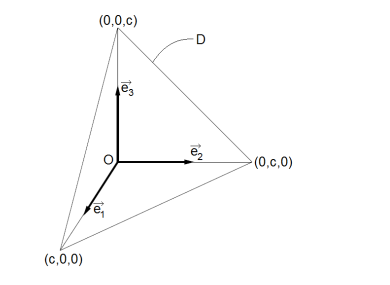
\includegraphics[width=0.45\textwidth]{images/contraintes.png}
\end{center}
\end{boiteexercice}

\begin{boitecorrige}
Le tenseur de Cauchy est symétrique : il y a 6 inconnues $\sigma_{11},\sigma_{22},\sigma_{33},\sigma_{12},\sigma_{13},\sigma_{23}$.

\textbf{Termes diagonaux.} Sur la face de normale sortante $-\vec{e}_1$, le vecteur contrainte est $\vec{T}(-\vec{e}_1)=-\overline{\overline{\sigma}}\cdot\vec{e}_1 = (-\sigma_{11},-\sigma_{12},-\sigma_{13})^T$. La composante normale (projection sur $-\vec{e}_1$) vaut $\sigma_{11}$. La surface de cette facette triangulaire est $S = c^2/2$, donc :
\[
F_1 = S\,\sigma_{11} \Longrightarrow \sigma_{11} = \frac{2F_1}{c^2}
\]
Par des raisonnements identiques sur les deux autres facettes :
\[
\sigma_{22} = \frac{2F_2}{c^2}, \qquad \sigma_{33} = \frac{2F_3}{c^2}
\]

\textbf{Termes hors-diagonaux.} La face inclinée a pour normale unitaire sortante $\vec{n} = \frac{1}{\sqrt{3}}(\vec{e}_1+\vec{e}_2+\vec{e}_3)$ et pour surface $S' = c^2\sqrt{3}/2$. Le vecteur contrainte est :
\[
\vec{T}(\vec{n}) = \frac{1}{\sqrt{3}}\begin{pmatrix}\sigma_{11}+\sigma_{12}+\sigma_{13}\\\sigma_{12}+\sigma_{22}+\sigma_{23}\\\sigma_{13}+\sigma_{23}+\sigma_{33}\end{pmatrix}
\]
La force sur cette facette vaut $\vec{G} = S'\,\vec{T}(\vec{n})$.

En substituant les termes diagonaux et en résolvant le système :
\[
\begin{cases}
\sigma_{12}+\sigma_{13} = (2G_1-2F_1)/c^2\\[2pt]
\sigma_{12}+\sigma_{23} = (2G_2-2F_2)/c^2\\[2pt]
\sigma_{13}+\sigma_{23} = (2G_3-2F_3)/c^2
\end{cases}
\]
En ajoutant les trois équations et en divisant par 2 :
\[
\sigma_{12}+\sigma_{13}+\sigma_{23} = \frac{(G_1+G_2+G_3)-(F_1+F_2+F_3)}{c^2}.
\]

En soustrayant chaque équation, on obtient finalement :
\begin{align*}
\sigma_{12} &= \frac{(G_1-F_1)+(G_2-F_2)-(G_3-F_3)}{c^2}\\
\sigma_{13} &= \frac{(G_1-F_1)-(G_2-F_2)+(G_3-F_3)}{c^2}\\
\sigma_{23} &= \frac{-(G_1-F_1)+(G_2-F_2)+(G_3-F_3)}{c^2}
\end{align*}
\end{boitecorrige}

\subsection*{Exercice 16 - Cisaillement simple \niveau{\facile}}

\begin{boiteexercice}
Un bloc élastique cubique de côté $a$, soumis à un cisaillement simple dans le plan $(x,y)$, a pour tenseur des contraintes :
\[
\sigma = \begin{pmatrix} 0 & \tau & 0 \\ \tau & 0 & 0 \\ 0 & 0 & 0 \end{pmatrix}.
\]
\begin{enumerate}
  \item Calculer les contraintes principales et les directions principales.
  \item Tracer le cercle de Mohr et déterminer la contrainte tangentielle maximale.
  \item Pour $\tau = 50\;\text{MPa}$, donner les valeurs des contraintes principales.
\end{enumerate}
\end{boiteexercice}

\begin{boitecorrige}

\textbf{1. Contraintes principales.}

Le polynôme caractéristique de $\sigma$ est $\det(\sigma - \lambda I) = -\lambda(\lambda^2 - \tau^2) = 0$, dont les racines sont :
\[
\sigma_1 = \tau, \quad \sigma_2 = -\tau, \quad \sigma_3 = 0.
\]
Les directions principales associées dans le plan $(x,y)$ sont à $\pm 45°$ des axes $x$ et $y$ :
\[
\hat{e}_1 = \frac{1}{\sqrt{2}}(\hat{e}_x + \hat{e}_y), \quad \hat{e}_2 = \frac{1}{\sqrt{2}}(\hat{e}_x - \hat{e}_y).
\]

\textbf{2. Cercle de Mohr.}

Dans le plan $(\sigma, \tau)$, le cercle de Mohr dans le plan de cisaillement a pour centre $(0, 0)$ et rayon $\tau$. Le cercle passe par les points $(\pm\tau, 0)$ (contraintes principales) et $(0, \pm\tau)$ (plans à 45°). La contrainte tangentielle maximale est donc :
\[
\tau_\text{max} = \tau.
\]

\textbf{3. Application numérique.}

Pour $\tau = 50\;\text{MPa}$ :
\[
\sigma_1 = +50\;\text{MPa}, \quad \sigma_2 = -50\;\text{MPa}, \quad \sigma_3 = 0.
\]
C'est un état de \emph{traction pure} dans la direction à $+45°$ et \emph{compression pure} dans la direction à $-45°$. Cette propriété est exploitée pour expliquer pourquoi un matériau fragile en cisaillement casse selon des plans à 45° (failure en traction).

\reponse{$\sigma_{1,2} = \pm\tau$, directions à $\pm 45°$ ; $\tau_\text{max} = \tau$}
\end{boitecorrige}

\subsection*{Exercice 17 - Équation de Navier-Stokes incompressible \niveau{\difficile}}

\begin{boiteexercice}
On considère un écoulement incompressible newtonien de densité $\rho$ et de viscosité dynamique $\mu$, régi par l'équation de Navier-Stokes :
\[
\rho\!\left(\frac{\partial\vec{v}}{\partial t} + (\vec{v}\cdot\grad)\vec{v}\right) = -\grad p + \mu\,\Delta\vec{v} + \rho\vec{f}.
\]
\begin{enumerate}
  \item Énoncer l'équation de continuité pour un écoulement incompressible.
  \item Montrer que pour un écoulement permanent ($\partial_t\vec{v}=0$) et sans forces volumiques ($\vec{f}=0$), la pression se calcule à partir de $\vec{v}$ par une équation de Poisson.
  \item Cas d'application : écoulement de Poiseuille plan entre deux plaques parallèles distantes de $2h$, gradient de pression $-G$. Donner le profil $v_x(y)$ et le débit volumique par unité de largeur.
\end{enumerate}
\end{boiteexercice}

\begin{boitecorrige}

\textbf{1. Continuité.}

La conservation de la masse pour un fluide incompressible ($\rho = $ cste) donne :
\[
\div\vec{v} = 0.
\]

\textbf{2. Équation de Poisson pour la pression.}

Pour un écoulement permanent sans forces volumiques :
\[
\rho(\vec{v}\cdot\grad)\vec{v} = -\grad p + \mu\,\Delta\vec{v}.
\]
En prenant la divergence des deux côtés et utilisant $\div\vec{v} = 0$ :
\[
\div\!\left[(\vec{v}\cdot\grad)\vec{v}\right] = -\Delta p + \mu\,\div(\Delta\vec{v}) = -\Delta p + \mu\,\Delta(\div\vec{v}) = -\Delta p.
\]
Donc :
\[
\Delta p = -\rho\,\div\!\left[(\vec{v}\cdot\grad)\vec{v}\right].
\]
C'est une équation de Poisson pour $p$, dont le second membre est connu dès que $\vec{v}$ est donné. Elle est utilisée dans les méthodes numériques de projection (Chorin) pour imposer l'incompressibilité.

\textbf{3. Écoulement de Poiseuille plan.}

Entre deux plaques en $y=\pm h$, le profil est unidirectionnel $\vec{v} = v_x(y)\hat{e}_x$. L'équation stationnaire devient :
\[
0 = -\frac{\d p}{\d x} + \mu\frac{\d^2 v_x}{\d y^2}.
\]
Avec $\d p/\d x = -G$ (gradient de pression constant) et $v_x(\pm h) = 0$ (non-glissement), on intègre deux fois :
\[
v_x(y) = \frac{G}{2\mu}(h^2 - y^2).
\]
Le profil est parabolique, maximal au centre ($v_\text{max} = Gh^2/(2\mu)$). Le débit volumique par unité de largeur :
\[
Q/L = \int_{-h}^{h} v_x(y)\,\d y = \frac{G}{2\mu}\!\left[h^2\cdot 2h - \frac{2h^3}{3}\right] = \frac{2Gh^3}{3\mu}.
\]
La vitesse moyenne est $\bar{v} = Q/(2hL) = Gh^2/(3\mu) = \tfrac{2}{3}v_\text{max}$.

\reponse{$v_x(y) = \dfrac{G}{2\mu}(h^2-y^2)$, \quad $Q/L = \dfrac{2Gh^3}{3\mu}$}
\end{boitecorrige}

\subsection*{Exercice 18 - Onde longitudinale dans une barre élastique \niveau{\moyen}}

\begin{boiteexercice}
On considère une barre élastique homogène de module d'Young $E$ et de masse volumique $\rho$, occupant l'axe $x\in[0,L]$. On note $u(x,t)$ le déplacement longitudinal.
\begin{enumerate}
  \item Établir l'équation d'onde par un bilan de forces sur un élément $\d x$.
  \item Donner la vitesse de propagation $c$ de l'onde.
  \item Application : barre en acier ($E = 200\;\text{GPa}$, $\rho = 7800\;\text{kg\,m}^{-3}$). Calculer $c$.
\end{enumerate}
\end{boiteexercice}

\begin{boitecorrige}

\textbf{1. Équation d'onde.}

Sur un élément $\d x$ de section $S$, la force à gauche est $F(x) = S\sigma_{xx} = SE\,\partial_x u$ (loi de Hooke 1D). Celle à droite est $F(x+\d x) = F(x) + \partial_x F\,\d x$. La masse est $\rho S\,\d x$. Par Newton :
\[
\rho S\,\d x\,\frac{\partial^2 u}{\partial t^2} = \partial_x F\,\d x = SE\,\frac{\partial^2 u}{\partial x^2}\,\d x.
\]
En simplifiant :
\[
\frac{\partial^2 u}{\partial t^2} = \frac{E}{\rho}\,\frac{\partial^2 u}{\partial x^2}.
\]

\textbf{2. Vitesse de propagation.}

L'équation est de type d'Alembert avec :
\[
c = \sqrt{E/\rho}.
\]

\textbf{3. Application acier.}

\[
c = \sqrt{\frac{200\times 10^9}{7800}} \approx 5064\;\text{m\,s}^{-1}.
\]
C'est la vitesse du son dans l'acier (valeur typique $5000$--$6000\;\text{m\,s}^{-1}$ selon l'alliage). On peut comparer avec la vitesse du son dans l'air ($\sim 340\;\text{m\,s}^{-1}$) : la barre solide transmet les vibrations 15 fois plus vite.

\reponse{$c = \sqrt{E/\rho} \approx 5\;\text{km\,s}^{-1}$ pour l'acier}
\end{boitecorrige}

\subsection*{Exercice 19 - Équilibre d'un barrage poids \niveau{\moyen}}

\begin{boiteexercice}
Un barrage poids triangulaire de hauteur $H$ et de largeur à la base $B$ retient une eau de densité $\rho_e$ sur sa face verticale amont. La masse volumique du béton est $\rho_b$.
\begin{enumerate}
  \item Calculer la résultante des forces de pression de l'eau sur le barrage.
  \item Calculer le moment de renversement par rapport au pied aval.
  \item Condition de non-renversement : $B/H \ge ?$ en fonction de $\rho_b/\rho_e$.
\end{enumerate}
\end{boiteexercice}

\begin{boitecorrige}

\textbf{1. Résultante des forces de pression.}

La pression hydrostatique à profondeur $z$ (depuis la surface libre) vaut $p(z) = \rho_e g z$. Sur la face verticale de hauteur $H$, la force par unité de largeur est :
\[
F = \int_0^H p(z)\,\d z = \rho_e g \frac{H^2}{2}.
\]
Le point d'application est à $2H/3$ de la surface libre, soit $H/3$ au-dessus de la base.

\textbf{2. Moment de renversement.}

Le moment de la force $F$ par rapport au pied aval (situé à la base, côté eau) vaut :
\[
M_\text{renv} = F \times \frac{H}{3} = \frac{\rho_e g H^3}{6}.
\]

\textbf{3. Condition de stabilité.}

Le poids du barrage par unité de largeur (triangle de hauteur $H$ et base $B$) :
\[
P = \rho_b g \frac{BH}{2}.
\]
Le centre de gravité du triangle est à $B/3$ du pied aval. Le moment stabilisant :
\[
M_\text{stab} = P \times \frac{B}{3} = \rho_b g \frac{BH}{2}\cdot\frac{B}{3} = \frac{\rho_b g B^2 H}{6}.
\]
Condition de non-renversement ($M_\text{stab} \ge M_\text{renv}$) :
\[
\frac{\rho_b g B^2 H}{6} \ge \frac{\rho_e g H^3}{6} \quad\Rightarrow\quad \frac{B^2}{H^2} \ge \frac{\rho_e}{\rho_b} \quad\Rightarrow\quad \frac{B}{H} \ge \sqrt{\frac{\rho_e}{\rho_b}}.
\]
Pour $\rho_b/\rho_e \approx 2{,}4$ (béton/eau), on obtient $B/H \ge 1/\sqrt{2{,}4} \approx 0{,}65$. En pratique, on prend $B/H \ge 0{,}7$ à $0{,}8$ pour inclure un coefficient de sécurité.

\reponse{$\dfrac{B}{H} \ge \sqrt{\dfrac{\rho_e}{\rho_b}} \approx 0{,}65$ pour béton/eau}
\end{boitecorrige}

\subsection*{Exercice 20 - Tenseur des déformations et rotationnel \niveau{\difficile}}

\begin{boiteexercice}
Soit le champ de déplacement :
\[
\vec{u}(x,y,z) = (\alpha xy,\, \beta xz,\, \gamma yz)
\]
où $\alpha, \beta, \gamma$ sont des constantes petites.
\begin{enumerate}
  \item Calculer la matrice jacobienne $\grad\vec{u}$.
  \item En déduire le tenseur des petites déformations $\epsilon$ et le tenseur rotationnel $\omega$.
  \item Vérifier la compatibilité géométrique (équations de Saint-Venant).
\end{enumerate}
\end{boiteexercice}

\begin{boitecorrige}

\textbf{1. Jacobienne.}

\[
\grad\vec{u} = \begin{pmatrix}
\partial_x u_x & \partial_y u_x & \partial_z u_x \\
\partial_x u_y & \partial_y u_y & \partial_z u_y \\
\partial_x u_z & \partial_y u_z & \partial_z u_z
\end{pmatrix} = \begin{pmatrix}
\alpha y & \alpha x & 0 \\
0 & 0 & \beta x \\
0 & \gamma z & \gamma y
\end{pmatrix}.
\]

\textbf{2. Déformations et rotation.}

Le tenseur des déformations (partie symétrique) :
\[
\epsilon = \frac{1}{2}(\grad\vec{u} + {}^t\!\grad\vec{u}) = \begin{pmatrix}
\alpha y & \alpha x/2 & 0 \\
\alpha x/2 & 0 & \beta x/2 + \gamma z/2 \\
0 & \beta x/2 + \gamma z/2 & \gamma y
\end{pmatrix}.
\]
Le tenseur rotation (partie antisymétrique) :
\[
\omega = \frac{1}{2}(\grad\vec{u} - {}^t\!\grad\vec{u}) = \begin{pmatrix}
0 & \alpha x/2 & 0 \\
-\alpha x/2 & 0 & \beta x/2 - \gamma z/2 \\
0 & -\beta x/2 + \gamma z/2 & 0
\end{pmatrix}.
\]
Le vecteur rotation associé est $\vec{\Omega} = \tfrac{1}{2}\rot\vec{u} = \tfrac{1}{2}\bigl(\partial_y u_z - \partial_z u_y,\, \partial_z u_x - \partial_x u_z,\, \partial_x u_y - \partial_y u_x\bigr) = \tfrac{1}{2}(\gamma z,\, 0,\, -\alpha x)$.

\textbf{3. Compatibilité de Saint-Venant.}

Les équations de compatibilité assurent que les $\epsilon_{ij}$ proviennent bien d'un champ de déplacement unique. Elles s'écrivent :
\[
\partial_{kl}\epsilon_{ij} + \partial_{ij}\epsilon_{kl} = \partial_{ik}\epsilon_{jl} + \partial_{jl}\epsilon_{ik}.
\]
Pour le champ donné, par exemple $\partial_y\epsilon_{xx} = \alpha$, $\partial_{xy}\epsilon_{xy} = \alpha/2$. Vérifions une équation :
\[
\partial_{yy}\epsilon_{xx} + \partial_{xx}\epsilon_{yy} = 0 + 0 = 0, \qquad 2\partial_{xy}\epsilon_{xy} = 2\times\frac{\alpha}{2} = \alpha.
\]
Pour compatibilité : $0 = \alpha$, soit $\alpha = 0$. Cela signifie que le champ $\vec{u}$ n'est physiquement compatible que si $\alpha = 0$. Plus généralement, les équations de Saint-Venant imposent ici $\alpha = \beta = \gamma = 0$ : le champ n'est pas physiquement réalisable en petites déformations. C'est un exemple pédagogique de l'importance des conditions de compatibilité.

\reponse{$\epsilon_{ij} = \tfrac{1}{2}(\partial_i u_j + \partial_j u_i)$ ; champ non compatible sauf si $\alpha=\beta=\gamma=0$}
\end{boitecorrige}

\ifdefined\inMainDoc\else\end{document}\fi


% ================================================================
%  UE 9 : OPTIQUE PHYSIQUE
% ================================================================
\newpage
\thispagestyle{empty}
\begin{tikzpicture}[remember picture, overlay]
  \fill[gray!12] ([xshift=1.5cm, yshift=3cm]current page.south west)
    rectangle ([xshift=-1.5cm, yshift=-3cm]current page.north east);
  \draw[line width=3pt] ([xshift=1.5cm,yshift=-3cm]current page.north west)
    -- ([xshift=-1.5cm,yshift=-3cm]current page.north east);
  \draw[line width=3pt] ([xshift=1.5cm,yshift=3cm]current page.south west)
    -- ([xshift=-1.5cm,yshift=3cm]current page.south east);
  \node[align=center] at (current page.center) {%
    {\fontsize{34}{42}\bfseries\selectfont OPTIQUE PHYSIQUE}\\[1.2cm]
    {\large\itshape Interférences - Diffraction}\\[0.4cm]
    {\large\itshape Réseaux - Polarisation}\\[1.8cm]
    {\normalsize Licence 3 - UE 9}
  };
  \node[anchor=south west] at ([xshift=2cm,yshift=2cm]current page.south west)
    {\large\bfseries UE 9};
\end{tikzpicture}
\newpage

\addcontentsline{toc}{section}{OPTIQUE PHYSIQUE}
\ifdefined\inMainDoc\else
\documentclass[12pt,a4paper]{article}
% ================================================================
%  PRÉAMBULE COMMUN - ANNALES CORRIGÉES
%  Université de Kara - FaST - Licence Fondamentale MPC
%  Design optimisé impression noir et blanc
% ================================================================

% -- ENCODAGE & LANGUE --
\usepackage[utf8]{inputenc}
\usepackage[T1]{fontenc}
\usepackage[french]{babel}
\usepackage{lmodern}
\usepackage{microtype}

% -- MISE EN PAGE --
\usepackage[a4paper, top=2.8cm, bottom=2.5cm, left=2.5cm, right=2.5cm, headheight=14pt]{geometry}
\usepackage{setspace}
\setstretch{1.2}
\usepackage{parskip}
\setlength{\parindent}{1.2em}
\setlength{\parskip}{4pt}

% -- MATHS --
\usepackage{amsmath, amssymb, mathtools, amsthm}
\usepackage{mathrsfs}
\usepackage{dsfont}
\usepackage{bm}
\usepackage{cancel}
\usepackage{textcomp}
% Définition de \oiint (intégrale de surface fermée) sans package supplémentaire
\newcommand{\oiint}{\mathop{\iint\!\!\!\!\!\!\!\bigcirc}\limits}

% -- PHYSIQUE & CHIMIE --
\usepackage{physics}
\usepackage{siunitx}
% Lorsque physics est chargé, siunitx omet \qty. On le restaure ici :
\AtBeginDocument{\RenewCommandCopy\qty\SI}
\sisetup{locale = FR, detect-all, output-decimal-marker={,}}
% Commande de substitution pour les unités posant problème avec pdflatex
% (ohm, degreeCelsius, micro, angstrom, percent utilisent des caractères non-ASCII)
\newcommand{\qtyohm}[1]{\ensuremath{\num{#1}\,\Omega}}
\newcommand{\qtydegc}[1]{\ensuremath{\num{#1}\,{}^\circ\text{C}}}
\newcommand{\qtyangstrom}[1]{\ensuremath{\num{#1}\,\text{\AA}}}
\newcommand{\qtypercent}[1]{\ensuremath{\num{#1}\,\%}}
\newcommand{\qtyum}[1]{\ensuremath{\num{#1}\,\mu\text{m}}}
\usepackage[version=4]{mhchem}

% -- GRAPHISMES --
\usepackage{graphicx}
\usepackage{float}
\usepackage{caption}
\usepackage{subcaption}
\usepackage{wrapfig}
\usepackage{tikz}
\usetikzlibrary{calc, arrows.meta, patterns, shapes.geometric}
\usepackage{pgfplots}
\pgfplotsset{compat=1.18}

% -- TABLEAUX --
\usepackage{booktabs}
\usepackage{array}
\usepackage{tabularx}
\usepackage{multirow}

% -- LISTES --
\usepackage{enumitem}
\setlist[enumerate]{topsep=3pt, itemsep=2pt, parsep=0pt}
\setlist[itemize]{topsep=3pt, itemsep=2pt, parsep=0pt, label={.}}

% -- BOÎTES (noir et blanc) --
\usepackage{mdframed}
\usepackage{tcolorbox}
\tcbuselibrary{skins, breakable, theorems}

% Boîte EXERCICE : encadré avec filet épais, fond blanc
\newmdenv[
  linewidth=1.2pt,
  linecolor=black,
  roundcorner=3pt,
  skipabove=10pt,
  skipbelow=6pt,
  innertopmargin=8pt,
  innerbottommargin=8pt,
  innerleftmargin=10pt,
  innerrightmargin=10pt,
  backgroundcolor=white,
  frametitle={\bfseries\small Exercice},
  frametitlealignment=\raggedright,
  frametitleaboveskip=4pt,
  frametitlebelowskip=4pt,
]{boiteexercice}

% Boîte CORRIGÉ : fond gris très clair + filet fin
\newmdenv[
  linewidth=0.6pt,
  linecolor=black,
  leftline=true,
  rightline=false,
  topline=false,
  bottomline=false,
  linecolor=black,
  innerleftmargin=12pt,
  innerrightmargin=8pt,
  innertopmargin=6pt,
  innerbottommargin=6pt,
  backgroundcolor=gray!8,
  skipabove=4pt,
  skipbelow=8pt,
]{boitecorrige}

% Boîte RÉSUMÉ DE COURS : double encadré
\newmdenv[
  linewidth=0.8pt,
  linecolor=black,
  roundcorner=2pt,
  backgroundcolor=gray!12,
  innertopmargin=10pt,
  innerbottommargin=10pt,
  innerleftmargin=12pt,
  innerrightmargin=12pt,
  skipabove=12pt,
  skipbelow=8pt,
]{boiteresume}

% Boîte ATTENTION/REMARQUE : barre gauche épaisse
\newmdenv[
  leftline=true,
  rightline=false,
  topline=false,
  bottomline=false,
  linewidth=3pt,
  linecolor=black,
  backgroundcolor=gray!5,
  innerleftmargin=12pt,
  innerrightmargin=8pt,
  innertopmargin=5pt,
  innerbottommargin=5pt,
  skipabove=6pt,
  skipbelow=6pt,
]{boiteremarque}

% -- DIFFICULTÉ DES EXERCICES --
\newcommand{\facile}{$\star$}
\newcommand{\moyen}{$\star\!\star$}
\newcommand{\difficile}{$\star\!\star\!\star$}
\newcommand{\niveau}[1]{\hfill\textbf{#1}\hspace{2pt}}

% -- EN-TÊTES ET PIEDS DE PAGE --
\usepackage{fancyhdr}
\pagestyle{fancy}
\fancyhf{}
\renewcommand{\headrulewidth}{0.5pt}
\renewcommand{\footrulewidth}{0.3pt}

% -- HYPERLIENS --
\usepackage[hidelinks]{hyperref}
\hypersetup{
    colorlinks=false,
    pdftitle={Annale Corrigée - Licence MPC - Université de Kara}
}

% -- TITRES --
\usepackage{titlesec}
\titleformat{\section}{\Large\bfseries}{\thesection.}{0.8em}{}[\vspace{2pt}\hrule\vspace{4pt}]
\titleformat{\subsection}{\large\bfseries}{\thesubsection.}{0.7em}{}
\titleformat{\subsubsection}{\normalsize\bfseries}{\thesubsubsection.}{0.6em}{}

% -- THÉORÈMES --
\theoremstyle{definition}
\newtheorem{defn}{Définition}[section]
\newtheorem{prop}{Propriété}[section]
\newtheorem{thm}{Théorème}[section]
\newtheorem{corol}{Corollaire}[section]
\newtheorem{exemple}{Exemple}[section]

% -- COMMANDES MATHÉMATIQUES UTILES --
\newcommand{\vect}[1]{\overrightarrow{#1}}
\newcommand{\R}{\mathbb{R}}
\newcommand{\N}{\mathbb{N}}
\newcommand{\Z}{\mathbb{Z}}
\newcommand{\C}{\mathbb{C}}
\renewcommand{\d}{\mathrm{d}}
\newcommand{\deriv}[2]{\dfrac{\d #1}{\d #2}}
\newcommand{\dpart}[2]{\dfrac{\partial #1}{\partial #2}}
\newcommand{\rot}{\overrightarrow{\mathrm{rot}}\,}
\renewcommand{\div}{\mathrm{div}\,}
\renewcommand{\grad}{\overrightarrow{\mathrm{grad}}\,}
\newcommand{\e}{\mathrm{e}}
\newcommand{\ii}{\mathrm{i}}
\renewcommand{\Tr}{\mathrm{Tr}}

% Numérotation des équations par section
\numberwithin{equation}{section}

% -- RÉSULTATS ENCADRÉS --
\newcommand{\res}[1]{\[\boxed{#1}\]}

% -- REMARQUE INLINE --
\newcommand{\rmq}[1]{\begin{boiteremarque}\textbf{Remarque.} #1\end{boiteremarque}}

% -- MISE EN VALEUR DU RÉSULTAT FINAL --
\newcommand{\reponse}[1]{%
  \begin{center}
    \fbox{\begin{minipage}{0.92\textwidth}\centering #1\end{minipage}}
  \end{center}%
}


\lhead{\small\textit{Optique Physique - Licence 3}}
\rhead{\small\textit{FaST, Université de Kara}}
\cfoot{\thepage}

\begin{document}
\fi

\begin{center}
  {\LARGE\bfseries OPTIQUE PHYSIQUE}\\[0.3cm]
  {\normalsize Licence 3 - Physique}\\[0.1cm]
  \rule{0.7\textwidth}{0.8pt}
\end{center}

\section*{Résumé du cours}

\begin{boiteresume}

\textbf{1. Lumière cohérente et interférences.} Deux ondes $E_1 = E_0\cos(\omega t + \varphi_1)$ et $E_2 = E_0\cos(\omega t + \varphi_2)$ sont cohérentes si leur déphasage $\Delta\varphi = \varphi_1-\varphi_2$ est constant. L'intensité résultante est :
\[
I = 4I_0\cos^2\!\left(\frac{\Delta\varphi}{2}\right)
\]
avec $\Delta\varphi = \frac{2\pi}{\lambda}\delta$ ($\delta$ : différence de marche optique). Franges brillantes si $\delta = k\lambda$, sombres si $\delta = (2k+1)\lambda/2$.

\textbf{2. Expérience des fentes d'Young.} Deux fentes distantes de $a$ éclairées par une source à distance $D$. Position des franges : $y_k = k\lambda D/a$. Interfrange : $i = \lambda D/a$.

\textbf{3. Diffraction.} La diffraction de Fraunhofer par une fente de largeur $b$ donne une figure d'intensité :
\[
I(\theta) = I_0\left(\frac{\sin(\beta/2)}{\beta/2}\right)^2, \quad \beta = \frac{2\pi b\sin\theta}{\lambda}
\]
Minimum (extinction) : $b\sin\theta = m\lambda$ ($m\neq0$ entier).

\textbf{4. Réseau de diffraction.} Un réseau de $N$ fentes espacées du pas $p$ donne des maxima principaux dans les directions $p\sin\theta = m\lambda$ (ordre $m$). Le pouvoir de résolution : $\mathcal{R} = mN$.

\textbf{5. Polarisation.} La loi de Malus : un faisceau polarisé linéairement d'intensité $I_0$ passe par un polariseur faisant un angle $\theta$ avec la direction de polarisation : $I = I_0\cos^2\theta$.

\end{boiteresume}

\newpage
\section{Interférences lumineuses}

\subsection*{Exercice 1 - Fentes d'Young \niveau{\facile}}

\begin{boiteexercice}
Dans une expérience de fentes d'Young, les deux fentes sont distantes de $a = \qty{0.5}{mm}$ et l'écran est placé à $D = \qty{1.5}{m}$. On utilise une lumière de longueur d'onde $\lambda = \qty{589}{nm}$ (jaune sodium).
\begin{enumerate}
  \item Calculer l'interfrange $i$.
  \item À quelle position sur l'écran se trouve la 3\textsuperscript{e} frange brillante (ordre $k=3$) ?
  \item La source s'élève de $h=\qty{0.2}{mm}$ par rapport à l'axe optique. Quel est l'effet sur les franges ?
\end{enumerate}
\end{boiteexercice}

\begin{boitecorrige}
\textbf{1.} $i = \dfrac{\lambda D}{a} = \dfrac{589\times10^{-9}\times1{,}5}{0{,}5\times10^{-3}} = \qty{1.767}{mm}$.

\textbf{2.} Position de la frange brillante d'ordre $k=3$ :
\[
y_3 = 3i = 3\times\qty{1.767}{mm} = \qty{5.30}{mm}
\]

\textbf{3.} Si la source se déplace de $h$ vers le haut, la différence de marche devient $\delta = \frac{ay}{D} - \frac{ah}{D_s}$ où $D_s$ est la distance source-fentes. L'ensemble du système de franges se translate de $\Delta y = -\frac{Dh}{D_s}$ vers le bas. La périodicité (interfrange) est inchangée.
\end{boitecorrige}

\subsection*{Exercice 2 - Lame à faces parallèles et coins d'air \niveau{\moyen}}

\begin{boiteexercice}
Un coin d'air est formé par deux lames de verre plates, dont l'une est légèrement inclinée d'un angle $\alpha = 2'$ (minutes d'arc). On observe les franges en lumière monochromatique de longueur d'onde $\lambda = \qty{550}{nm}$.
\begin{enumerate}
  \item Calculer l'interfrange $i$ (distance entre deux franges brillantes consécutives).
  \item Combien de franges observe-t-on sur une longueur de \qty{20}{mm} ?
  \item La frange centrale (d'ordre 0) est-elle brillante ou sombre ? Expliquer.
\end{enumerate}
\end{boiteexercice}

\begin{boitecorrige}
\textbf{1.} La différence de marche au point situé à $x$ du contact est $\delta = 2e(x) = 2x\tan\alpha \approx 2x\alpha$ (avec $\alpha$ en radians). L'interfrange correspond à $\Delta\delta = \lambda$, soit $2\alpha\Delta x = \lambda$ :
\[
i = \Delta x = \frac{\lambda}{2\alpha} = \frac{550\times10^{-9}}{2\times(2/60)\times(\pi/180)} = \frac{550\times10^{-9}}{1{,}164\times10^{-4}} \approx \qty{4.73}{mm}
\]

\textbf{2.} Nombre de franges : $N = \frac{20}{4{,}73} \approx 4{,}2$, donc environ 4 franges.

\textbf{3.} La frange centrale (en $x=0$, épaisseur nulle) est une frange \textbf{sombre}. En effet, lors de la réflexion sur la lame du dessous (verre plus dense), il y a un déphasage de $\pi$ (changement de signe du champ réfléchi). La différence de marche effective en $e=0$ est $\delta = 0+\lambda/2$, ce qui donne une extinction.
\end{boitecorrige}

\section{Diffraction}

\subsection*{Exercice 3 - Diffraction par une fente \niveau{\moyen}}

\begin{boiteexercice}
Un faisceau laser de longueur d'onde $\lambda = \qty{633}{nm}$ éclaire une fente de largeur $b = \qty{0.1}{mm}$. L'écran est à $D = \qty{2}{m}$.
\begin{enumerate}
  \item Calculer la position du premier minimum de diffraction.
  \item Quelle est la largeur de la tache centrale ?
  \item Comparer la largeur de la tache à la largeur de la fente.
\end{enumerate}
\end{boiteexercice}

\begin{boitecorrige}
\textbf{1.} Premier minimum : $b\sin\theta_1 = \lambda$, donc $\sin\theta_1 = \lambda/b = 633\times10^{-9}/(0{,}1\times10^{-3}) = 6{,}33\times10^{-3}$. Pour de petits angles : $\theta_1\approx\sin\theta_1$, et la position sur l'écran est :
\[
y_1 = D\tan\theta_1 \approx D\theta_1 = 2\times6{,}33\times10^{-3} = \qty{12.66}{mm}
\]

\textbf{2.} La tache centrale s'étend de $-y_1$ à $+y_1$ : largeur $= 2y_1 = \qty{25.3}{mm}$.

\textbf{3.} Rapport largeur tache/largeur fente : $25{,}3\,\text{mm}/0{,}1\,\text{mm} = 253$. La diffraction est d'autant plus importante que la fente est étroite : la tache est 253 fois plus large que la fente.
\end{boitecorrige}

\subsection*{Exercice 4 - Réseau de diffraction \niveau{\moyen}}

\begin{boiteexercice}
Un réseau de diffraction possède $N = 500$ traits/mm. On l'éclaire normalement avec la lumière blanche visible ($\lambda\in[400\,\text{nm},\;700\,\text{nm}]$).
\begin{enumerate}
  \item Calculer le pas du réseau $p$.
  \item À quel angle sort la raie verte ($\lambda=\qty{550}{nm}$) au premier ordre ?
  \item Le spectre du premier ordre chevauche-t-il celui du second ordre ? (Calculer l'angle de la raie violette au 2\textsuperscript{e} ordre et celui de la raie rouge au 1\textsuperscript{er} ordre.)
  \item Quel est le pouvoir de résolution à l'ordre 2 pour un réseau de 3\,cm de large ?
\end{enumerate}
\end{boiteexercice}

\begin{boitecorrige}
\textbf{1.} $p = 1/500\,\text{mm}^{-1} = \qtyum{2}$.

\textbf{2.} Condition de réseau : $p\sin\theta = m\lambda$. Au 1\textsuperscript{er} ordre ($m=1$) pour $\lambda=\qty{550}{nm}$ :
$\sin\theta = 550\times10^{-9}/(2\times10^{-6}) = 0{,}275$, donc $\theta = 15{,}96°\approx16°$.

\textbf{3.} Raie violette au 2\textsuperscript{e} ordre : $\sin\theta = 2\times400\times10^{-9}/(2\times10^{-6}) = 0{,}4$, $\theta=23{,}6°$.
Raie rouge au 1\textsuperscript{er} ordre : $\sin\theta = 700\times10^{-9}/(2\times10^{-6}) = 0{,}35$, $\theta=20{,}5°$.

Le spectre du 1\textsuperscript{er} ordre s'étend de $\approx11{,}5°$ (violet) à $\approx20{,}5°$ (rouge). Le 2\textsuperscript{e} ordre commence à $\approx23{,}6°$. Les spectres ne se chevauchent pas.

\textbf{4.} Nombre de traits sur 3\,cm : $N = 500\times30 = 15000$ traits. Pouvoir de résolution : $\mathcal{R} = mN = 2\times15000 = 30\,000$. On peut résoudre deux longueurs d'onde séparées de $\Delta\lambda = \lambda/\mathcal{R} = 550/30000 \approx \qty{0.018}{nm}$.
\end{boitecorrige}

\subsection*{Exercice 5 - Polarisation : loi de Malus \niveau{\difficile}}

\begin{boiteexercice}
Un faisceau de lumière naturelle d'intensité $I_0$ traverse successivement :
\begin{itemize}[nosep]
  \item Un premier polariseur $P_1$ (orientation $0°$).
  \item Un second polariseur $P_2$ (orientation $\theta$).
  \item Un troisième polariseur $P_3$ (orientation $90°$).
\end{itemize}
\begin{enumerate}
  \item Exprimer l'intensité $I_3$ sortant de $P_3$ en fonction de $I_0$ et $\theta$.
  \item Pour quelle valeur de $\theta$ l'intensité $I_3$ est-elle maximale ?
  \item Comparer avec l'intensité si $P_2$ était absent.
\end{enumerate}
\end{boiteexercice}

\begin{boitecorrige}
\textbf{1.} Après $P_1$ (lumière naturelle $\to$ polarisée) : $I_1 = I_0/2$ (polariseur extrait la moitié de l'intensité).

Après $P_2$ (angle $\theta$ avec $P_1$) : $I_2 = I_1\cos^2\theta = \frac{I_0}{2}\cos^2\theta$.

Après $P_3$ (angle $90°-\theta$ avec $P_2$) : $I_3 = I_2\cos^2(90°-\theta) = \frac{I_0}{2}\cos^2\theta\sin^2\theta$.

En utilisant $\sin(2\theta)=2\sin\theta\cos\theta$ :
\[
\boxed{I_3 = \frac{I_0}{8}\sin^2(2\theta)}
\]

\textbf{2.} Maximum pour $\sin^2(2\theta)=1$, soit $\theta=45°$ : $I_{3,\max} = \dfrac{I_0}{8}$.

\textbf{3.} Sans $P_2$, les polariseurs $P_1$ et $P_3$ sont croisés (angle $90°$) : $I_3=\frac{I_0}{2}\cos^2(90°)=0$.

Le polariseur intermédiaire, placé à $45°$, permet de « faire passer » de la lumière à travers deux polariseurs croisés. C'est un résultat contre-intuitif : ajouter un polariseur augmente l'intensité transmise (de 0 à $I_0/8$).
\end{boitecorrige}


\section{Interférences - dispositifs complémentaires}

\subsection*{Exercice 6 - Déplacement latéral de la source dans l'expérience des trous de Young \niveau{\moyen}}

\begin{boiteexercice}
On réalise l'expérience de Young : une plaque P est percée de deux fentes étroites $F_1$ et $F_2$ identiques, parallèles et distantes de $a$. Une fente source F très fine est éclairée par une lumière monochromatique de longueur d'onde $\lambda$. Toutes les fentes sont dans des plans perpendiculaires au plan de la figure. On note $x'$ la distance de F au centre $O_1$ du plan S. S est à une distance $D'$ de P. À la distance $D \gg a$ du plan des fentes, on place un écran vertical.
\begin{enumerate}
  \item Soient deux rayons issus de la source et arrivant sur l'écran à une distance $x$ de O, après être passés respectivement par $F_1$ et $F_2$. Déterminer la différence de marche et le déphasage entre ces rayons.
  \item Comment est modifiée l'image sur l'écran par rapport à la situation usuelle où F est équidistante de $F_1$ et $F_2$ ? Donner la position du centre de la figure d'interférence.
\end{enumerate}
\begin{figure}[H]
\centering
\includegraphics[width=0.7\textwidth]{images/op5.jpg}
\end{figure}
\end{boiteexercice}

\begin{boitecorrige}
La source est décentrée : les deux rayons parcourent des distances différentes pour atteindre $F_1$ et $F_2$. On note $\delta'$ la différence de marche entre les deux rayons en provenance de F, et $\delta$ la différence de marche classique au point M de l'écran.

\begin{enumerate}
  \item \textbf{Calcul de $\delta$.} On obtient le résultat classique :
  \[
  \delta = \frac{ax}{D}
  \]
  \textbf{Calcul de $\delta'$.} On note $\theta'$ l'angle $\widehat{F_2 F_1 H'}$. Dans le triangle $(F O_2 O_1)$, $\tan\theta' = x'/D'$, donc :
  \[
  \delta' = a\sin\theta' \approx \frac{ax'}{D'}
  \]
  La différence de marche totale et le déphasage valent :
  \[
  \Delta = \delta + \delta' = a\!\left(\frac{x}{D}+\frac{x'}{D'}\right), \qquad
  \varphi = \frac{2\pi}{\lambda}\,a\!\left(\frac{x}{D}+\frac{x'}{D'}\right)
  \]
\begin{figure}[H]
\centering
\includegraphics[width=0.7\textwidth]{images/op6.jpg}
\end{figure}

  \item L'intensité sur l'écran est $I(x) = I_0(1+\cos\varphi)$. Dans le cas usuel ($x'=0$), la frange centrale est en $x=0$. Ici, la figure d'interférence est \textbf{décalée} : la frange centrale (où $\varphi=0$) est en $x = -x'D/D'$. L'interfrange reste inchangé.
\end{enumerate}
\end{boitecorrige}

\subsection*{Exercice 7 - Biprisme de Fresnel \niveau{\moyen}}

\begin{boiteexercice}
Une onde lumineuse plane de longueur d'onde $\lambda$ rencontre normalement la face d'entrée d'un biprisme transparent : le premier verre, d'indice $n$, est un biprisme de petit angle $A$, suivi d'une lame à faces parallèles d'indice $n'$. Qu'observe-t-on sur un écran E disposé perpendiculairement à la direction incidente ? On se place dans l'approximation des petits angles.

Application numérique : $A = 5{,}0°$, $n = 1{,}520$, $n' = 1{,}500$, $\lambda = 0{,}7\;\mu\text{m}$.
\begin{figure}[H]
\centering
\includegraphics[width=0.5\textwidth]{images/op10.jpg}
\end{figure}
\end{boiteexercice}

\begin{boitecorrige}
Il s'agit de l'interférence de deux ondes planes dont les vecteurs d'onde forment un angle $2\theta_2$. On suit un rayon dévié vers le bas. À la sortie du biprisme (loi de Descartes au petit angle avec $i = A$) :
\begin{figure}[H]
\centering
\includegraphics[width=0.5\textwidth]{images/op11.jpg}
\end{figure}
\[
\theta_1 = i' - i = \left(\frac{n}{n'}-1\right)A = \frac{(n-n')A}{n'}
\]
Puis le rayon traverse la lame d'indice $N$ ; on montre que :
\[
\theta_2 = n'\theta_1 = (n-n')A
\]
L'interférence donne des franges d'interfrange :
\[
i = \frac{\lambda}{2\sin\theta_2} \approx \frac{\lambda}{2\theta_2} = \frac{\lambda}{2(n-n')A}
\]
\begin{figure}[H]
\centering
\includegraphics[width=0.5\textwidth]{images/op12.jpg}
\end{figure}
\textbf{A.N.} $A = 5° = 0{,}0873\;\text{rad}$, $(n-n') = 0{,}020$ :
\[
i = \frac{0{,}7\times10^{-6}}{2\times0{,}020\times0{,}0873} \approx \qty{0.20}{mm}
\]
On observe sur l'écran une figure d'interférence constituée de franges alternativement sombres et brillantes de pas $i \approx 0{,}20\;\text{mm}$.
\end{boitecorrige}

\subsection*{Exercice 8 - Miroir de Lloyd \niveau{\moyen}}

\begin{boiteexercice}
On note $d$ la distance du bord du miroir à l'écran, $a$ la distance de la source S au miroir, et $\ell$ la distance horizontale de S au bord du miroir.
\begin{enumerate}
  \item Justifier qu'on observe sur l'écran l'interférence de deux ondes et préciser lesquelles. Comparer les amplitudes.
  \item Représenter la zone d'interférence.
  \item Déterminer la distance entre les deux sources virtuelles $S_1$ et $S_2$ équivalentes. Quelle est leur distance à l'écran ?
  \item En déduire l'expression de l'intensité sur l'écran. Quelle est la forme des franges ?
\end{enumerate}
\begin{figure}[H]
\centering
\includegraphics[width=0.5\textwidth]{images/op13.jpg}
\end{figure}
\end{boiteexercice}

\begin{boitecorrige}
\begin{enumerate}
  \item Sur l'écran, on observe l'interférence de l'onde issue \textit{directement} de S et de celle qui, issue de S, se réfléchit sur le miroir. C'est un phénomène par division du front d'onde. Les deux ondes ont même amplitude $A$.
\begin{figure}[H]
\centering
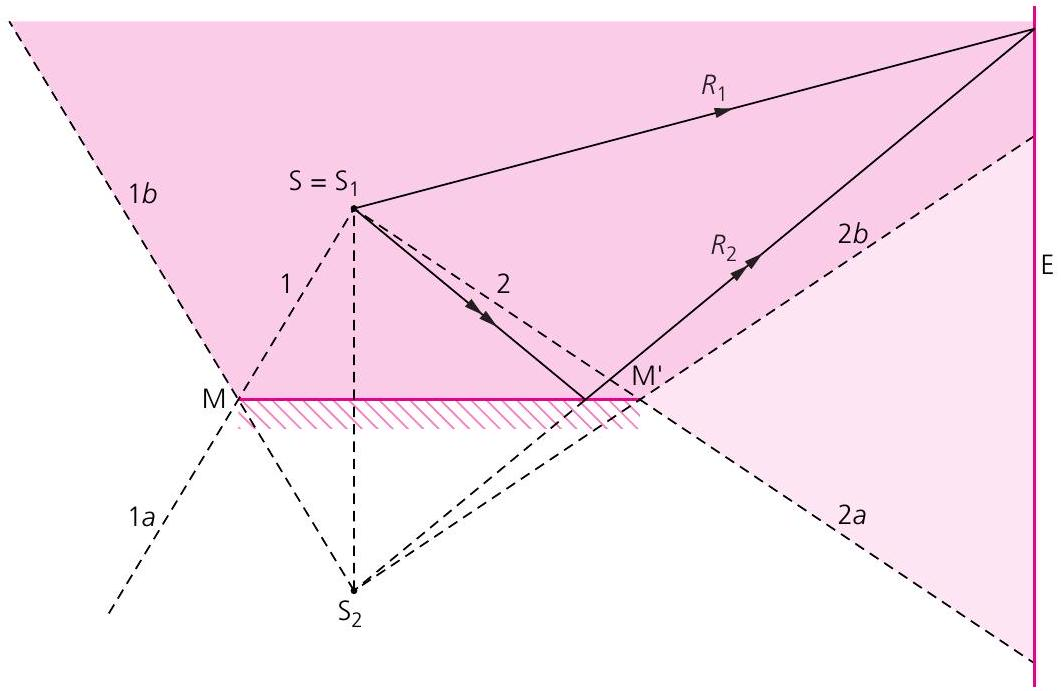
\includegraphics[width=0.7\textwidth]{images/op14.jpg}
\end{figure}
  \item La zone d'interférence correspond à la région où les deux sous-faisceaux se recouvrent (indiquée en sombre sur la figure).

  \item Les deux sous-faisceaux sont coniques de sommets $S_1 \equiv S$ et $S_2$ (image de S par le miroir). Les deux sources virtuelles sont distantes de $2a$ parallèlement à l'écran. Leur distance à l'écran est $(\ell + d)$.

  \item On applique le résultat des trous de Young :
  \[
  I(x) = I_0\!\left[1+\cos\!\left(2\pi\,\frac{2a}{\lambda(\ell+d)}\,x\right)\right]
  \]
  On observe des franges brillantes et sombres d'intensité continûment variable sur la partie de l'écran où les deux sous-faisceaux se croisent.
\end{enumerate}
\end{boitecorrige}

\subsection*{Exercice 9 - Biprisme de Fresnel en Lumière Blanche \niveau{\difficile}}

\begin{boiteexercice}
On considère un biprisme d'angle au sommet $\alpha$ (avec $\alpha$ petit) et d'indice $n = 1{,}5$. Le biprisme est éclairé par une source lumineuse ponctuelle S. On observe la figure d'interférences sur un écran à la distance $L = 3\;\text{m}$ de son sommet. La source, à la distance $D = 2\;\text{cm}$ du sommet, émet de la lumière blanche ($400\;\text{nm} < \lambda < 750\;\text{nm}$).
\begin{figure}[H]
\centering
\includegraphics[width=0.8\textwidth]{images/op22.png}
\end{figure}
\begin{enumerate}
  \item Rappeler les caractéristiques de la figure d'interférence en lumière monochromatique (largeur de la zone d'interférence et nombre de franges sombres).
  \item Combien de cannelures sombres observe-t-on au point M en lumière blanche ? Faire l'application numérique pour $x = 10\;\text{mm}$.
\end{enumerate}
\end{boiteexercice}

\begin{boitecorrige}
\begin{enumerate}
\item \textbf{Lumière monochromatique.} Le biprisme crée deux sources virtuelles $S_1$ et $S_2$ symétriques par rapport à S.
\begin{figure}[H]
\centering
\includegraphics[width=0.8\textwidth]{images/op23.png}
\end{figure}
La déviation d'un prisme de petit angle $\alpha$ est $\beta = (n-1)\alpha$. Les sources virtuelles sont séparées de :
\[
a = S_1 S_2 = 2(n-1)\alpha D
\]
\begin{figure}[H]
\centering
\includegraphics[width=0.8\textwidth]{images/op24.png}
\end{figure}
La largeur de la zone d'interférence est $d = 2(n-1)\alpha L$. L'interfrange est :
\[
i = \frac{\lambda(D+L)}{a} = \frac{\lambda(D+L)}{2(n-1)\alpha D}
\]
Le nombre de franges sombres est $N \approx d/i$.

\item \textbf{Lumière blanche --- cannelures sombres.} La différence de marche au point M(x) est :
\[
\delta(M) = \frac{a\,x}{D+L} = \frac{2(n-1)\alpha D\,x}{D+L}
\]
Les cannelures sombres correspondent aux longueurs d'onde éteintes vérifiant $\delta = (2k+1)\lambda/2$, soit :
\[
\lambda_k = \frac{2\delta(M)}{2k+1}
\]
La condition pour que $\lambda_k$ soit dans le visible ($\lambda_v = 400\;\text{nm}$, $\lambda_r = 750\;\text{nm}$) donne :
\[
\frac{2\delta(M)}{(2k+1)\lambda_r} \leq 1 \leq \frac{2\delta(M)}{(2k+1)\lambda_v}
\quad\Longrightarrow\quad
\frac{\delta(M)}{\lambda_r} - \frac{1}{2} \leq k \leq \frac{\delta(M)}{\lambda_v} - \frac{1}{2}
\]
\textbf{A.N.} Pour $x = 10\;\text{mm}$, avec les valeurs de l'énoncé on trouve $15 \leq k \leq 28$, soit \textbf{14 cannelures sombres}.
\end{enumerate}
\end{boitecorrige}

\subsection*{Exercice 10 - Coin d'air et cohérence temporelle \niveau{\moyen}}

\begin{boiteexercice}
Une onde lumineuse monochromatique plane de longueur d'onde $\lambda_0$ rencontre un coin de verre d'indice $n$ dont les faces font un angle $\alpha$ très petit. Le plan d'incidence est perpendiculaire à l'arête du coin, et l'angle d'incidence est $i$.
\begin{enumerate}
  \item Déterminer l'interfrange $\Delta x$ de la figure d'interférence obtenue par réflexion sur les faces de la lame lorsque $i = 0$.
  \item La source émet une lumière de spectre de largeur $\Delta\lambda$ centré sur $\lambda$. La longueur de cohérence est $L = \lambda^2/\Delta\lambda$. Les franges disparaissent quand la différence de marche dépasse $L$. Calculer $\alpha$ et la finesse $\lambda/\Delta\lambda$ si les franges disparaissent à la distance $l = 8\;\text{cm}$ du sommet.

Données : $\lambda = 0{,}55\;\mu\text{m}$, $i = 0$, $\Delta x = 0{,}21\;\text{mm}$, $n = 1{,}5$.
\end{enumerate}
\begin{figure}[H]
\centering
\includegraphics[width=0.7\textwidth]{images/op26.png}
\end{figure}
\end{boiteexercice}

\begin{boitecorrige}
\begin{enumerate}
  \item L'intensité lumineuse pour le coin de verre à incidence normale s'écrit :
  \[
  I(x) \approx \frac{I_0}{2}(1+\cos(2kn\alpha x))
  \]
  L'interfrange est donc :
  \[
  \Delta x = \frac{\lambda}{2n\alpha}
  \]

  \item \textbf{A.N.} $\alpha = \dfrac{\lambda}{2n\Delta x} = \dfrac{0{,}55\times10^{-6}}{2\times1{,}5\times0{,}21\times10^{-3}} = 8{,}7\times10^{-4}\;\text{rad}$.

  À la distance $l$ du sommet, la différence de marche est $\delta \approx 2nl\alpha$. Quand les franges disparaissent : $\delta = L = \lambda^2/\Delta\lambda$. L'ordre d'interférence correspondant est $P_l = \delta/\lambda = \lambda/\Delta\lambda$, soit :
  \[
  \frac{\Delta\lambda}{\lambda} = \frac{\lambda}{2nl\alpha} = \frac{\Delta x}{l} = \frac{0{,}21\;\text{mm}}{80\;\text{mm}} = 2{,}6\times10^{-3}
  \]
  La finesse est $\lambda/\Delta\lambda \approx 385$.
\end{enumerate}
\end{boitecorrige}

\subsection*{Exercice 11 - Les anneaux de Newton \niveau{\moyen}}

\begin{boiteexercice}
On considère le dispositif des anneaux de Newton. On utilise une lentille plan-convexe de rayon $R$ et d'angle d'ouverture $\theta$, dont la face courbe repose en O sur un plan de verre $Ox$. Il existe entre le plan et la lentille une lame d'air d'épaisseur $e(x)$ variable, avec $e(0) = 0$. On suppose $e \ll R$. Une source monochromatique étendue éclaire la lentille en incidence normale.
\begin{figure}[H]
\centering
\includegraphics[width=0.8\textwidth]{images/op27.png}
\end{figure}
\begin{enumerate}
  \item Rappeler quelles ondes interférent et préciser le lieu de localisation des franges.
  \item Calculer la différence de marche $\delta(x)$.
  \item Exprimer $e(x)$ en fonction de $x$. Décrire la figure d'interférence. Quel aspect a la frange centrale ?
\end{enumerate}
\end{boiteexercice}

\begin{boitecorrige}
\begin{enumerate}
  \item Les rayons qui interférent sont : $R_1$, directement réfléchis par la face courbe de la lame d'air (face courbe de la lentille), et $R_2$, réfractés dans la lame d'air puis réfléchis par la face plane. Les rayons se coupent sur la face courbe : les franges sont localisées sur la lentille (en pratique, sur le plan $Ox$ car $e$ est très petit).

  \item $R_2$ parcourt $2e(x)$ dans l'air et subit une réflexion d'un milieu d'indice 1 vers un milieu d'indice $n > 1$ : déphasage $\pi$ équivalent à $\lambda/2$. Donc :
  \[
  \delta = 2e(x) + \frac{\lambda}{2}
  \]

  \item La lentille est une portion de sphère : $R^2 = x^2 + (R-e)^2$. Avec $e \ll R$ :
  \[
  e \approx \frac{x^2}{2R}
  \]
  L'intensité est :
  \[
  I(x) = I_0\!\left(1 - \cos\!\left(\frac{2\pi x^2}{\lambda R}\right)\right)
  \]
  Les zones d'égale intensité sont des cercles concentriques. Les franges sombres ont pour rayons $x_k = \sqrt{k R \lambda}$ avec $k$ entier. Les franges brillantes ont $x_k = \sqrt{(k+1/2)R\lambda}$. La frange centrale est sombre.
\end{enumerate}
\end{boitecorrige}

\section{Interféromètre de Michelson}

\subsection*{Exercice 12 - Franges de lames minces au Michelson \niveau{\difficile}}

\begin{boiteexercice}
Dans l'interféromètre de Michelson (séparatrice G infiniment mince), la source S est étendue et monochromatique ($\lambda = 0{,}5\;\mu\text{m}$).
\begin{enumerate}
  \item Depuis la position de référence ($IK_1 = IK_2$), on déplace $M_2$ de 1\,cm selon $x$. On observe dans le plan focal image d'une lentille $L$. Qu'observe-t-on ? Quelle est la variation de l'ordre d'interférence au centre si l'on place sur l'un des bras une lame mince d'épaisseur $7{,}5\;\mu\text{m}$ et d'indice $n = 1{,}5$ ?
  \item On revient à la position $IK_1 = IK_2$ et on fait pivoter $M_2$ d'un angle $\alpha$ très faible autour d'un axe passant par $K_2$. Qu'observe-t-on sur $M_1$ ? Exprimer l'éclairement en un point P de $M_1$ tel que $K_1 P = X$. Que vaut l'interfrange $i^*$ ?
\end{enumerate}
\begin{figure}[H]
\centering
\includegraphics[width=0.4\textwidth]{images/op30.png}
\end{figure}
\end{boiteexercice}

\begin{boitecorrige}
\begin{enumerate}
  \item Le système est équivalent à une lame d'air à faces parallèles d'épaisseur $e = 1\;\text{cm}$. Avec une source étendue, on observe des \textbf{anneaux} (franges d'égale inclinaison) dans le plan focal de $L$. La différence de marche est $\delta = 2e\cos i$. L'ordre au centre vaut $p_{\text{centre}} = 2e/\lambda = 2\times10^{-2}/(5\times10^{-7}) = 40\,000$.

  Avec la lame mince d'épaisseur $e'$ et d'indice $n$ : la variation d'ordre au centre est
  \[
  |\Delta p_{\text{centre}}| = \frac{2e'(n-1)}{\lambda} = \frac{2\times7{,}5\times10^{-6}\times(1{,}5-1)}{5\times10^{-7}} = 15
  \]
  Ainsi, 15 anneaux disparaissent (ou apparaissent) au centre.

  \item L'ensemble se comporte comme un coin d'air d'angle $\alpha$ dont l'arête passe par $K_1$. On observe des \textbf{franges d'égale épaisseur} (franges rectilignes parallèles). L'épaisseur de lame équivalente en un point $P$ tel que $K_1 P = X$ est $e = \alpha X$. L'éclairement est :
  \[
  I = 2I_0\!\left[1+\cos\!\left(\frac{4\pi\alpha X}{\lambda}\right)\right]
  \]
  L'interfrange est :
  \[
  i^* = \frac{\lambda}{2\alpha}
  \]
\end{enumerate}
\end{boitecorrige}

\subsection*{Exercice 13 - Réseau de diffraction : devise spectrale \niveau{\moyen}}

\begin{boiteexercice}
Un réseau de diffraction possède $N = 600$ traits par millimètre et une largeur utile $L = \qty{2}{cm}$.
\begin{enumerate}
  \item Calculer le pas $p$ du réseau.
  \item Pour la raie verte du mercure ($\lambda = \qty{546}{nm}$), déterminer l'angle $\theta$ de diffraction à l'ordre $m=1$.
  \item Calculer le pouvoir de résolution théorique $\mathcal{R}$ à l'ordre 1, puis en déduire la plus petite différence de longueurs d'onde $\Delta\lambda$ résolvable autour de \qty{546}{nm}.
  \item Application : le mercure émet un doublet jaune ($\lambda_1 = 577{,}0\;\text{nm}$ et $\lambda_2 = 579{,}1\;\text{nm}$). Le réseau peut-il séparer ce doublet à l'ordre 1 ?
\end{enumerate}
\end{boiteexercice}

\begin{boitecorrige}
\textbf{1.} Pas du réseau : $p = 1/N = 1/600\;\text{mm} \approx 1{,}667\;\mu\text{m}$.

\textbf{2.} Formule du réseau : $p\sin\theta = m\lambda$ avec $m=1$.
\[
\sin\theta = \frac{\lambda}{p} = \frac{546\times10^{-9}}{1{,}667\times10^{-6}} \approx 0{,}328 \implies \theta \approx 19{,}1^\circ
\]

\textbf{3.} Pouvoir de résolution à l'ordre $m$ : $\mathcal{R} = mN_\text{traits}$. Le nombre total de traits éclairés est $N_\text{traits} = N\times L = 600 \times 20 = 12000$. Donc :
\[
\mathcal{R} = 1 \times 12000 = 12000
\]
Plus petite différence résolvable :
\[
\Delta\lambda_\text{min} = \frac{\lambda}{\mathcal{R}} = \frac{546}{12000} \approx 0{,}046\;\text{nm}
\]

\textbf{4.} L'écart du doublet est $\Delta\lambda = 579{,}1 - 577{,}0 = 2{,}1\;\text{nm} \gg \Delta\lambda_\text{min}$. Oui, le réseau sépare le doublet à l'ordre 1 (et même à un ordre bien plus faible).
\reponse{$\theta \approx 19{,}1^\circ$, $\mathcal{R} = 12000$, $\Delta\lambda_\text{min} \approx 0{,}046\;\text{nm}$; le doublet est résolu.}
\end{boitecorrige}

\subsection*{Exercice 14 - Polarisation circulaire et lame quart d'onde \niveau{\moyen}}

\begin{boiteexercice}
Une lumière polarisée rectilignement selon $Ox$ traverse une lame quart d'onde dont les axes sont à $45^\circ$ de $Ox$. La longueur d'onde est $\lambda = \qty{632}{nm}$.
\begin{enumerate}
  \item Rappeler l'effet d'une lame quart d'onde sur une vibration polarisée rectilignement.
  \item Déterminer la nature de la lumière émergente.
  \item Comment modifier le dispositif pour obtenir une polarisation circulaire de sens opposé ?
\end{enumerate}
\end{boiteexercice}

\begin{boitecorrige}
\textbf{1.} Une lame quart d'onde introduit un déphasage de $\pi/2$ entre les composantes de la vibration selon les axes lent et rapide. Son épaisseur vérifie $(n_e - n_o)e = \lambda/4$.

\textbf{2.} La vibration incidente $\vec{E} = E_0\cos(\omega t)\,\hat{x}$ se décompose à parts égales sur les axes de la lame (orientés à $45^\circ$) :
\[
\vec{E}_\text{lent} = \frac{E_0}{\sqrt{2}}\cos(\omega t), \quad \vec{E}_\text{rapide} = \frac{E_0}{\sqrt{2}}\cos(\omega t)
\]
À la sortie, la composante rapide est en avance de $\pi/2$ :
\[
\vec{E}_\text{sortie} = \frac{E_0}{\sqrt{2}}\left[\cos(\omega t)\,\hat{e}_\text{lent} + \cos(\omega t - \pi/2)\,\hat{e}_\text{rapide}\right] = \frac{E_0}{\sqrt{2}}\left[\cos(\omega t)\,\hat{e}_\text{lent} + \sin(\omega t)\,\hat{e}_\text{rapide}\right]
\]
Le vecteur $\vec{E}$ tourne à vitesse angulaire $\omega$ en décrivant un cercle : la lumière est \textbf{polarisée circulairement}.

\textbf{3.} Pour inverser le sens de rotation (passer de droit à gauche), il suffit de tourner la lame de $90^\circ$ (échanger les axes lent et rapide), ou d'ajouter une deuxième lame quart d'onde identique orientée à $90^\circ$ de la première.
\reponse{Lumière émergente : polarisation circulaire. Pour inverser le sens : rotation de la lame de $90^\circ$.}
\end{boitecorrige}

\subsection*{Exercice 15 - Diffraction par une ouverture circulaire \niveau{\difficile}}

\begin{boiteexercice}
Un télescope a un miroir primaire de diamètre $D = \qty{50}{cm}$. On observe une étoile émettant à $\lambda = \qty{550}{nm}$.
\begin{enumerate}
  \item Rappeler l'expression du rayon angulaire $\theta_1$ du premier anneau sombre de la figure d'Airy.
  \item Calculer $\theta_1$ en radians et en secondes d'arc.
  \item Deux étoiles sont séparées angulairement par $\alpha = 0{,}5''$. Le télescope peut-il les séparer (critère de Rayleigh) ?
  \item Quel diamètre minimal faudrait-il pour résoudre un détail de $0{,}1''$ ?
\end{enumerate}
\end{boiteexercice}

\begin{boitecorrige}
\textbf{1.} Le premier zéro de la fonction d'Airy $J_1(x)/x$ est à $x = 1{,}22\,\pi$, soit :
\[
\theta_1 = \frac{1{,}22\,\lambda}{D}
\]

\textbf{2.} Application numérique :
\[
\theta_1 = \frac{1{,}22\times 550\times10^{-9}}{0{,}50} = 1{,}342\times10^{-6}\;\text{rad}
\]
\[
\theta_1 = \frac{1{,}342\times10^{-6}\times 180\times 3600}{\pi} \approx 0{,}277''
\]

\textbf{3.} Critère de Rayleigh : deux sources sont résolues si leur séparation angulaire $\alpha \geq \theta_1$. Ici $\alpha = 0{,}5'' > 0{,}277''$ : \textbf{oui}, le télescope résout les deux étoiles.

\textbf{4.} Pour résoudre $0{,}1'' = 0{,}1\times\pi/(180\times 3600) = 4{,}85\times10^{-7}\;\text{rad}$ :
\[
D_\text{min} = \frac{1{,}22\,\lambda}{\alpha} = \frac{1{,}22\times 550\times10^{-9}}{4{,}85\times10^{-7}} \approx 1{,}38\;\text{m}
\]
\reponse{$\theta_1 \approx 0{,}277''$, séparation possible pour $\alpha = 0{,}5''$ ; $D_\text{min} \approx 1{,}38\;\text{m}$ pour $0{,}1''$.}
\end{boitecorrige}

\subsection*{Exercice 16 - Trous d'Young en lumière non monochromatique \niveau{\difficile}}

\begin{boiteexercice}
On réalise une expérience de trous d'Young avec une source émettant deux longueurs d'onde $\lambda_1 = 589{,}0\;\text{nm}$ et $\lambda_2 = 589{,}6\;\text{nm}$ (doublet du sodium). Les fentes sont distantes de $a = 0{,}4\;\text{mm}$ et l'écran est à $D = 1{,}2\;\text{m}$.
\begin{enumerate}
  \item Calculer les interfranges $i_1$ et $i_2$ correspondant à chaque longueur d'onde.
  \item À partir de quelle position $x_k$ sur l'écran observe-t-on la première coïncidence des franges brillantes des deux longueurs d'onde ?
  \item En déduire la longueur de cohérence $\ell_c$ et le temps de cohérence $\tau_c$ du doublet.
\end{enumerate}
\end{boiteexercice}

\begin{boitecorrige}
\textbf{1.} Interfrange : $i = \lambda D/a$.
\[
i_1 = \frac{589{,}0\times10^{-9}\times 1{,}2}{0{,}4\times10^{-3}} \approx 1{,}767\;\text{mm}, \quad i_2 = \frac{589{,}6\times10^{-9}\times 1{,}2}{0{,}4\times10^{-3}} \approx 1{,}769\;\text{mm}
\]

\textbf{2.} Les franges brillantes coïncident quand $k_1 i_1 = k_2 i_2$ avec $k_1 \neq k_2$ (première coïncidence : $k_2 = k_1 + 1$). On cherche le plus petit $k$ tel que :
\[
k i_1 = (k+1) i_2 \quad\Longrightarrow\quad k(i_1-i_2) = i_2
\]
\[
k = \frac{i_2}{i_1 - i_2} = \frac{1{,}769}{1{,}769 - 1{,}767} \approx 884{,}5
\]
Position de la première coïncidence :
\[
x_k = k\,i_1 \approx 884 \times 1{,}767 \approx 1{,}56\;\text{m}
\]

\textbf{3.} La longueur de cohérence est la différence de marche correspondante :
\[
\ell_c = x_k\cdot\frac{a}{D} = 1{,}56 \times \frac{0{,}4\times10^{-3}}{1{,}2} \approx 0{,}52\;\text{mm}
\]
Temps de cohérence :
\[
\tau_c = \frac{\ell_c}{c} = \frac{0{,}52\times10^{-3}}{3\times10^8} \approx 1{,}7\;\text{ps}
\]
\reponse{$i_1 \approx 1{,}767\;\text{mm}$, $i_2 \approx 1{,}769\;\text{mm}$ ; $\ell_c \approx 0{,}52\;\text{mm}$, $\tau_c \approx 1{,}7\;\text{ps}$.}
\end{boitecorrige}

\subsection*{Exercice 17 - Polariseurs croisés et lame demi-onde \niveau{\moyen}}

\begin{boiteexercice}
Une lumière naturelle d'intensité $I_0$ traverse un polariseur $P_1$ (vertical), puis une lame demi-onde dont l'axe fait un angle $\alpha$ avec la verticale, puis un polariseur $P_2$ (horizontal, donc croisé avec $P_1$).
\begin{enumerate}
  \item Donner l'intensité après $P_1$.
  \item Décrire l'effet de la lame demi-onde sur la direction de polarisation.
  \item Calculer l'intensité finale $I_s$ après $P_2$ en fonction de $I_0$ et $\alpha$.
  \item Pour quelle valeur de $\alpha$ l'intensité transmise est-elle maximale ?
\end{enumerate}
\end{boiteexercice}

\begin{boitecorrige}
\textbf{1.} Lumière naturelle : $P_1$ transmet $I_0/2$.

\textbf{2.} Une lame demi-onde introduit un déphasage de $\pi$ entre les axes lent et rapide. Une vibration polarisée selon un angle $\alpha$ par rapport à l'axe rapide ressort symétrisée par rapport à cet axe : la nouvelle direction de polarisation fait l'angle $-\alpha$ (au lieu de $+\alpha$) avec l'axe rapide. Soit un angle total $2\alpha$ entre incident et émergent.

\textbf{3.} Après $P_1$ (vertical) : polarisation verticale. La lame demi-onde la fait pivoter de $2\alpha$ (par rapport à la verticale). $P_2$ est horizontal : l'intensité transmise par $P_2$ est $I\cos^2(90^\circ - 2\alpha) = I\sin^2(2\alpha)$ :
\[
I_s = \frac{I_0}{2}\sin^2(2\alpha)
\]

\textbf{4.} Maximum pour $\sin^2(2\alpha) = 1$, soit $2\alpha = 90^\circ$ ou $\alpha = 45^\circ$ :
\[
I_{s,\max} = \frac{I_0}{2}
\]
\reponse{$I_s = (I_0/2)\sin^2(2\alpha)$ ; maximum pour $\alpha = 45^\circ$, $I_{s,\max} = I_0/2$.}
\end{boitecorrige}

\subsection*{Exercice 18 - Interféromètre de Michelson : anneaux d'égale inclinaison \niveau{\difficile}}

\begin{boiteexercice}
Un interféromètre de Michelson réglé en lame d'air (épaisseur $e = 0{,}2\;\text{mm}$) est éclairé par une source étendue de longueur d'onde $\lambda = 546\;\text{nm}$.
\begin{enumerate}
  \item Donner l'expression de la différence de marche $\delta$ en fonction de l'angle d'incidence $i$.
  \item Calculer le rayon angulaire du $k$-ième anneau brillant.
  \item Calculer le nombre d'anneaux visibles dans un champ angulaire de $10^\circ$.
  \item Que se passe-t-il si on diminue $e$ vers 0 ?
\end{enumerate}
\end{boiteexercice}

\begin{boitecorrige}
\textbf{1.} Pour le Michelson en lame d'air :
\[
\delta = 2e\cos i
\]

\textbf{2.} Anneaux brillants : $\delta = k\lambda$, soit $\cos i_k = k\lambda/(2e)$. Pour $i$ petit, $\cos i \approx 1 - i^2/2$ :
\[
i_k \approx \sqrt{\frac{2(2e - k\lambda)}{2e}} = \sqrt{2\left(1 - \frac{k\lambda}{2e}\right)}
\]
L'ordre maximal $k_\text{max}$ correspond à $i=0$ : $k_\text{max} = 2e/\lambda = 2\times 0{,}2\times10^{-3}/546\times10^{-9} \approx 733$.

\textbf{3.} Pour $i = 10^\circ = 0{,}174\;\text{rad}$, $\cos i \approx 0{,}985$ :
\[
k_\text{min} = \frac{2e\cos i}{\lambda} = \frac{2\times 0{,}2\times10^{-3}\times 0{,}985}{546\times10^{-9}} \approx 722
\]
Nombre d'anneaux visibles : $k_\text{max} - k_\text{min} \approx 733 - 722 = 11$ anneaux.

\textbf{4.} Quand $e \to 0$, $k_\text{max} \to 0$ : les anneaux s'écartent vers l'extérieur et sortent du champ. À $e = 0$ (contact optique), le champ est uniforme (teinte plate).
\reponse{$\delta = 2e\cos i$ ; environ 11 anneaux dans un champ de $10^\circ$ ; les anneaux s'écartent quand $e\to 0$.}
\end{boitecorrige}

\subsection*{Exercice 19 - Spectre cannelé d'une lame mince \niveau{\moyen}}

\begin{boiteexercice}
Une lame de verre d'épaisseur $e = 0{,}5\;\text{mm}$ et d'indice $n = 1{,}5$ est éclairée en lumière blanche. On observe le spectre de la lumière transmise à l'aide d'un spectromètre.
\begin{enumerate}
  \item Donner l'expression de la différence de marche entre les rayons réfléchis deux fois et ceux qui traversent directement.
  \item Quelles longueurs d'onde sont éteintes (cannelures sombres) ?
  \item Calculer les deux premières longueurs d'onde éteintes dans le visible ($400$-$700\;\text{nm}$).
\end{enumerate}
\end{boiteexercice}

\begin{boitecorrige}
\textbf{1.} Différence de marche en transmission : $\delta = 2ne$ (la réflexion sur le verre n'introduit pas de déphasage supplémentaire en transmission).

\textbf{2.} Cannelures sombres (interférences destructives) : $\delta = (2k+1)\lambda/2$, soit :
\[
\lambda_k = \frac{2ne}{k+\frac{1}{2}} = \frac{4ne}{2k+1}, \quad k = 0, 1, 2, \ldots
\]

\textbf{3.} Application numérique : $4ne = 4\times 1{,}5 \times 0{,}5\times10^{-3} = 3\times10^{-3}\;\text{m} = 3000\;\mu\text{m}$.
\begin{itemize}[nosep]
  \item $k=4$ : $\lambda = 3000/9 \approx 333\;\text{nm}$ (UV)
  \item $k=5$ : $\lambda = 3000/11 \approx 273\;\text{nm}$ (UV, hors visible)
\end{itemize}
Pour le visible ($400$-$700\;\text{nm}$) : $400 \leq 3000/(2k+1) \leq 700$, soit $4{,}3 \leq 2k+1 \leq 7{,}5$, donc $2k+1 \in \{5, 7\}$, soit $k=2$ ($\lambda = 600\;\text{nm}$, jaune-orange) et $k=3$ ($\lambda \approx 428\;\text{nm}$, violet).
\reponse{Cannelures visibles : $\lambda \approx 600\;\text{nm}$ et $\lambda \approx 428\;\text{nm}$.}
\end{boitecorrige}

\subsection*{Exercice 20 - Réseau blazé et ordre de diffraction \niveau{\difficile}}

\begin{boiteexercice}
Un réseau blazé possède 1200 traits/mm, et est éclairé en incidence normale. L'angle de blaze est $\theta_b = 20^\circ$.
\begin{enumerate}
  \item Calculer le pas $p$.
  \item Déterminer la longueur d'onde de blaze à l'ordre $m=1$.
  \item Pour cette longueur d'onde, calculer l'angle de diffraction.
  \item Comparer l'efficacité du réseau blazé à celle d'un réseau classique (non blazé).
\end{enumerate}
\end{boiteexercice}

\begin{boitecorrige}
\textbf{1.} Pas : $p = 1/1200\;\text{mm} \approx 833\;\text{nm}$.

\textbf{2.} Longueur d'onde de blaze à l'ordre $m$ : $\lambda_b = 2p\sin\theta_b / m$.
\[
\lambda_b = 2\times 833\times10^{-9}\times \sin(20^\circ) \approx 2\times 833\times10^{-9}\times 0{,}342 \approx 570\;\text{nm}
\]

\textbf{3.} L'angle de diffraction pour $\lambda_b$ à l'ordre 1 vérifie $p\sin\theta = \lambda_b$ :
\[
\sin\theta = \frac{\lambda_b}{p} = \frac{570}{833} \approx 0{,}684 \implies \theta \approx 43{,}1^\circ
\]
C'est bien l'angle spéculaire par rapport à la face blazée ($\theta = 2\theta_b \approx 40^\circ$ environ, l'écart vient des approximations).

\textbf{4.} Le réseau blazé concentre l'énergie dans l'ordre $m=1$ à la longueur d'onde $\lambda_b$ (efficacité $\sim 80\%$), alors qu'un réseau classique (sinusoïdal) répartit l'énergie entre plusieurs ordres (efficacité $\sim 30$-$40\%$ par ordre). Le réseau blazé est donc beaucoup plus lumineux pour les applications spectrales.
\reponse{$p \approx 833\;\text{nm}$, $\lambda_b \approx 570\;\text{nm}$, $\theta \approx 43^\circ$ ; efficacité $\sim 80\%$ (vs $\sim 30$-$40\%$ sans blaze).}
\end{boitecorrige}

\newpage
\section*{Galerie d'illustrations d'optique physique}

\begin{figure}[H]
\centering
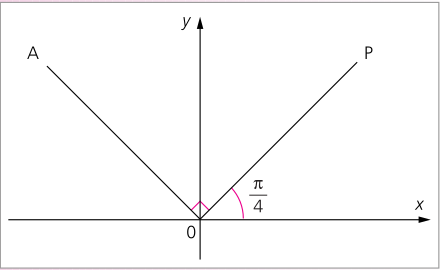
\includegraphics[width=0.7\textwidth]{images/optique_physique/op1.png}
\caption{Schéma du montage des fentes d'Young.}
\end{figure}

\begin{figure}[H]
\centering
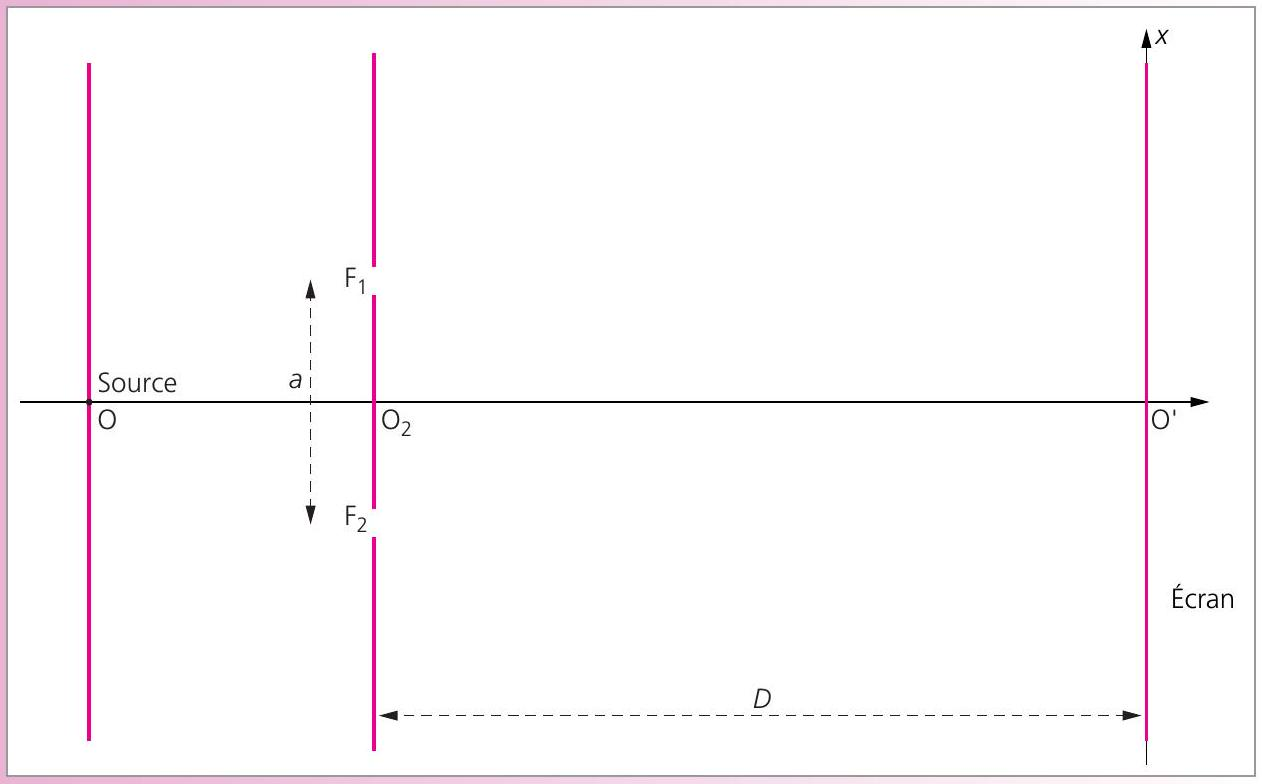
\includegraphics[width=0.7\textwidth]{images/optique_physique/op2.jpg}
\caption{Figure d'interférence observée sur l'écran.}
\end{figure}

\begin{figure}[H]
\centering
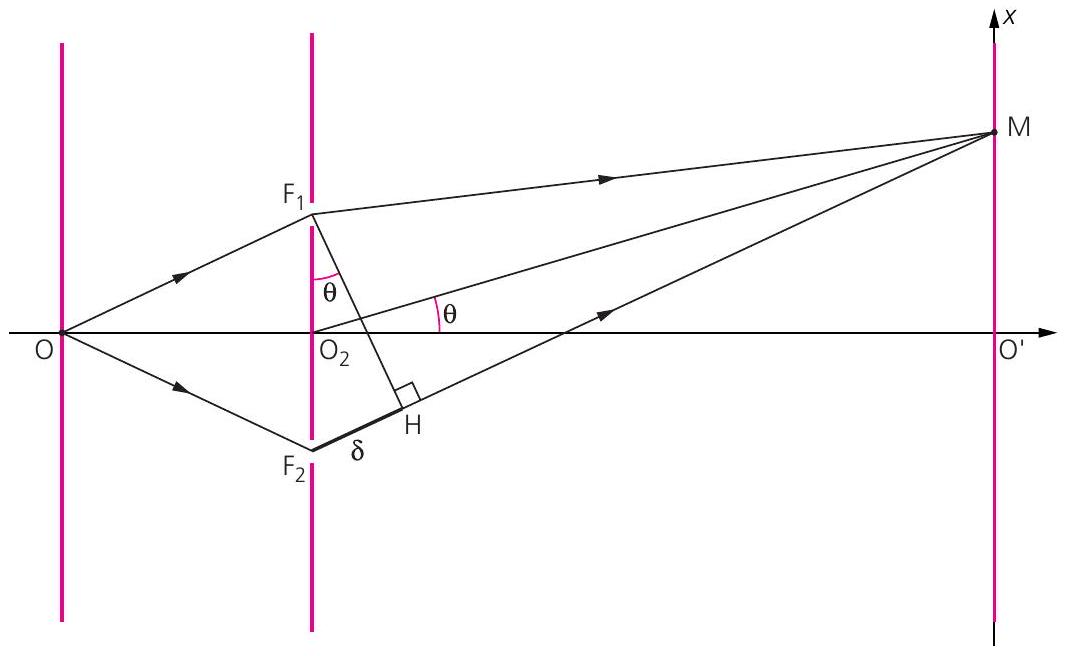
\includegraphics[width=0.7\textwidth]{images/optique_physique/op3.jpg}
\caption{Diffraction par une fente fine.}
\end{figure}

\begin{figure}[H]
\centering
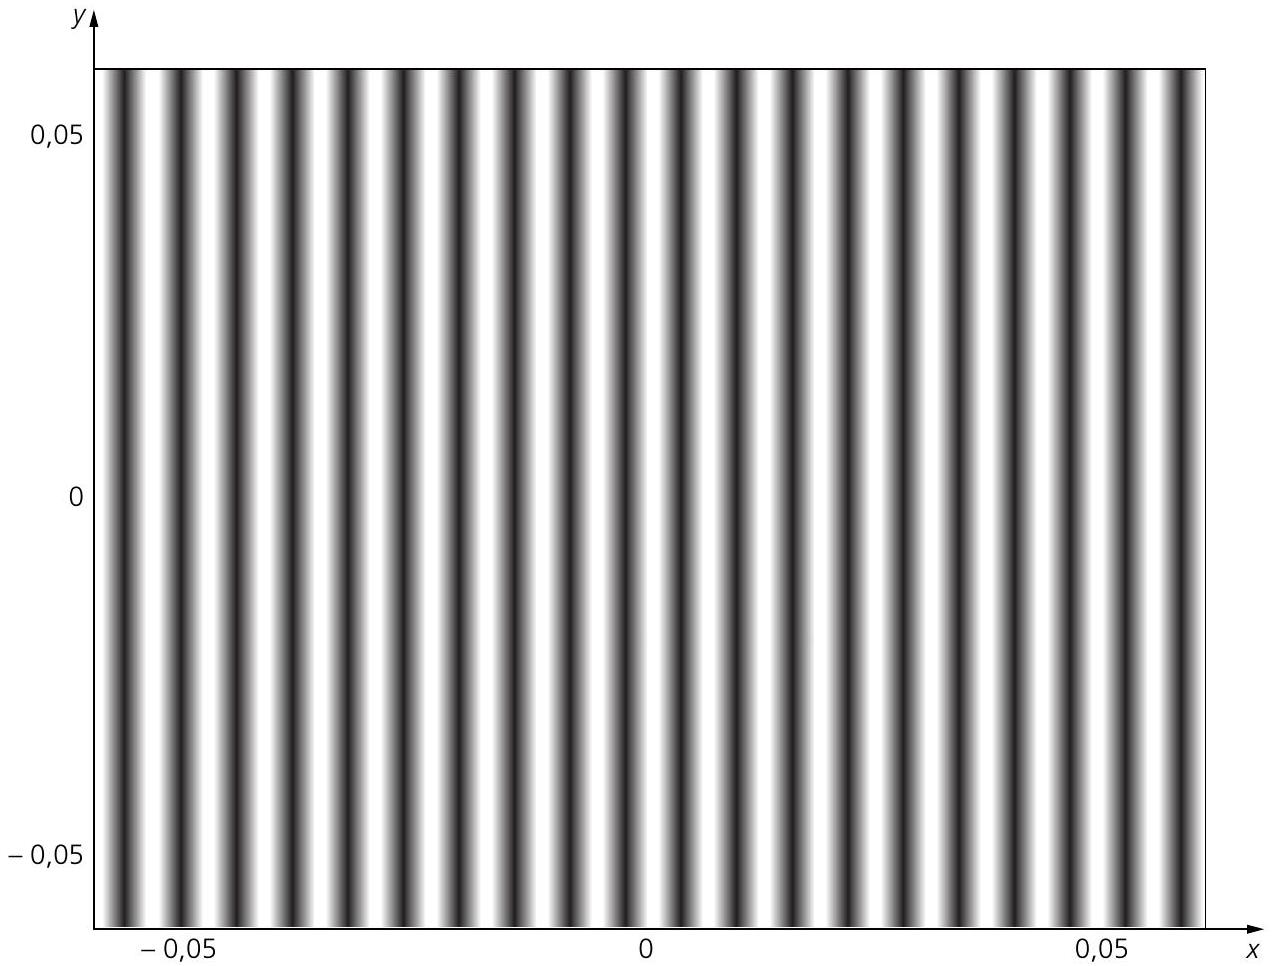
\includegraphics[width=0.7\textwidth]{images/optique_physique/op4.jpg}
\caption{Diffraction par une ouverture circulaire (figure d'Airy).}
\end{figure}

\begin{figure}[H]
\centering
\includegraphics[width=0.7\textwidth]{images/optique_physique/op5.jpg}
\caption{Réseau de diffraction : spectres d'ordres multiples.}
\end{figure}

\begin{figure}[H]
\centering
\includegraphics[width=0.7\textwidth]{images/optique_physique/op6.jpg}
\caption{Polarisation : loi de Malus.}
\end{figure}

\begin{figure}[H]
\centering
\includegraphics[width=0.7\textwidth]{images/optique_physique/op10.jpg}
\caption{Biprisme de Fresnel : géométrie.}
\end{figure}

\begin{figure}[H]
\centering
\includegraphics[width=0.7\textwidth]{images/optique_physique/op11.jpg}
\caption{Miroir de Lloyd : franges d'interférence.}
\end{figure}

\begin{figure}[H]
\centering
\includegraphics[width=0.7\textwidth]{images/optique_physique/op12.jpg}
\caption{Interféromètre de Michelson : montage.}
\end{figure}

\begin{figure}[H]
\centering
\includegraphics[width=0.7\textwidth]{images/optique_physique/op13.jpg}
\caption{Anneaux de Newton en lumière monochromatique.}
\end{figure}

\begin{figure}[H]
\centering
\includegraphics[width=0.7\textwidth]{images/optique_physique/op22.png}
\caption{Coin d'air : franges d'égale épaisseur.}
\end{figure}

\begin{figure}[H]
\centering
\includegraphics[width=0.7\textwidth]{images/optique_physique/op23.png}
\caption{Lame à faces parallèles : anneaux d'égale inclinaison.}
\end{figure}

\begin{figure}[H]
\centering
\includegraphics[width=0.7\textwidth]{images/optique_physique/op24.png}
\caption{Réseau de diffraction : spectre cannelé.}
\end{figure}

\begin{figure}[H]
\centering
\includegraphics[width=0.7\textwidth]{images/optique_physique/op26.png}
\caption{Diffraction de Fraunhofer par une fente.}
\end{figure}

\begin{figure}[H]
\centering
\includegraphics[width=0.7\textwidth]{images/optique_physique/op27.png}
\caption{Cohérence temporelle et longueur de cohérence.}
\end{figure}

\begin{figure}[H]
\centering
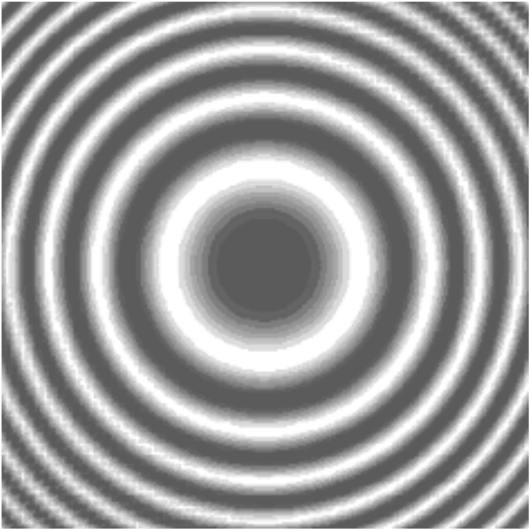
\includegraphics[width=0.7\textwidth]{images/optique_physique/op28.png}
\caption{Polarisation circulaire : composantes de la vibration.}
\end{figure}

\begin{figure}[H]
\centering
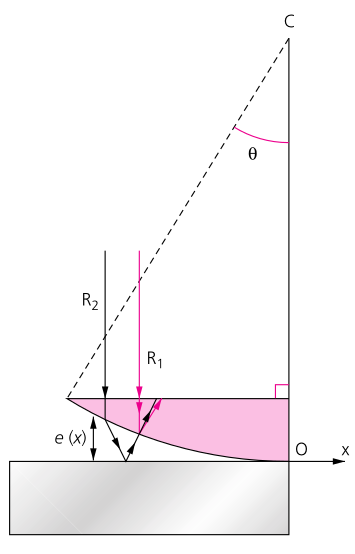
\includegraphics[width=0.7\textwidth]{images/optique_physique/op29.png}
\caption{Lame quart d'onde et demi-onde : principe.}
\end{figure}

\begin{figure}[H]
\centering
\includegraphics[width=0.7\textwidth]{images/optique_physique/op30.png}
\caption{Réseau blazé : géométrie et angle de blaze.}
\end{figure}

\ifdefined\inMainDoc\else\end{document}\fi


% ================================================================
%  UE 10 : PHYSIQUE MATHÉMATIQUE
% ================================================================
\newpage
\thispagestyle{empty}
\begin{tikzpicture}[remember picture, overlay]
  \fill[gray!12] ([xshift=1.5cm, yshift=3cm]current page.south west)
    rectangle ([xshift=-1.5cm, yshift=-3cm]current page.north east);
  \draw[line width=3pt] ([xshift=1.5cm,yshift=-3cm]current page.north west)
    -- ([xshift=-1.5cm,yshift=-3cm]current page.north east);
  \draw[line width=3pt] ([xshift=1.5cm,yshift=3cm]current page.south west)
    -- ([xshift=-1.5cm,yshift=3cm]current page.south east);
  \node[align=center] at (current page.center) {%
    {\fontsize{30}{38}\bfseries\selectfont PHYSIQUE MATHÉMATIQUE}\\[1.2cm]
    {\large\itshape Formes différentielles - EDP}\\[0.4cm]
    {\large\itshape Green-Riemann - Transformée de Fourier}\\[1.8cm]
    {\normalsize Licence 3 - UE 10}
  };
  \node[anchor=south west] at ([xshift=2cm,yshift=2cm]current page.south west)
    {\large\bfseries UE 10};
\end{tikzpicture}
\newpage

\addcontentsline{toc}{section}{PHYSIQUE MATHÉMATIQUE}
\ifdefined\inMainDoc\else
\documentclass[12pt,a4paper]{article}
% ================================================================
%  PRÉAMBULE COMMUN - ANNALES CORRIGÉES
%  Université de Kara - FaST - Licence Fondamentale MPC
%  Design optimisé impression noir et blanc
% ================================================================

% -- ENCODAGE & LANGUE --
\usepackage[utf8]{inputenc}
\usepackage[T1]{fontenc}
\usepackage[french]{babel}
\usepackage{lmodern}
\usepackage{microtype}

% -- MISE EN PAGE --
\usepackage[a4paper, top=2.8cm, bottom=2.5cm, left=2.5cm, right=2.5cm, headheight=14pt]{geometry}
\usepackage{setspace}
\setstretch{1.2}
\usepackage{parskip}
\setlength{\parindent}{1.2em}
\setlength{\parskip}{4pt}

% -- MATHS --
\usepackage{amsmath, amssymb, mathtools, amsthm}
\usepackage{mathrsfs}
\usepackage{dsfont}
\usepackage{bm}
\usepackage{cancel}
\usepackage{textcomp}
% Définition de \oiint (intégrale de surface fermée) sans package supplémentaire
\newcommand{\oiint}{\mathop{\iint\!\!\!\!\!\!\!\bigcirc}\limits}

% -- PHYSIQUE & CHIMIE --
\usepackage{physics}
\usepackage{siunitx}
% Lorsque physics est chargé, siunitx omet \qty. On le restaure ici :
\AtBeginDocument{\RenewCommandCopy\qty\SI}
\sisetup{locale = FR, detect-all, output-decimal-marker={,}}
% Commande de substitution pour les unités posant problème avec pdflatex
% (ohm, degreeCelsius, micro, angstrom, percent utilisent des caractères non-ASCII)
\newcommand{\qtyohm}[1]{\ensuremath{\num{#1}\,\Omega}}
\newcommand{\qtydegc}[1]{\ensuremath{\num{#1}\,{}^\circ\text{C}}}
\newcommand{\qtyangstrom}[1]{\ensuremath{\num{#1}\,\text{\AA}}}
\newcommand{\qtypercent}[1]{\ensuremath{\num{#1}\,\%}}
\newcommand{\qtyum}[1]{\ensuremath{\num{#1}\,\mu\text{m}}}
\usepackage[version=4]{mhchem}

% -- GRAPHISMES --
\usepackage{graphicx}
\usepackage{float}
\usepackage{caption}
\usepackage{subcaption}
\usepackage{wrapfig}
\usepackage{tikz}
\usetikzlibrary{calc, arrows.meta, patterns, shapes.geometric}
\usepackage{pgfplots}
\pgfplotsset{compat=1.18}

% -- TABLEAUX --
\usepackage{booktabs}
\usepackage{array}
\usepackage{tabularx}
\usepackage{multirow}

% -- LISTES --
\usepackage{enumitem}
\setlist[enumerate]{topsep=3pt, itemsep=2pt, parsep=0pt}
\setlist[itemize]{topsep=3pt, itemsep=2pt, parsep=0pt, label={.}}

% -- BOÎTES (noir et blanc) --
\usepackage{mdframed}
\usepackage{tcolorbox}
\tcbuselibrary{skins, breakable, theorems}

% Boîte EXERCICE : encadré avec filet épais, fond blanc
\newmdenv[
  linewidth=1.2pt,
  linecolor=black,
  roundcorner=3pt,
  skipabove=10pt,
  skipbelow=6pt,
  innertopmargin=8pt,
  innerbottommargin=8pt,
  innerleftmargin=10pt,
  innerrightmargin=10pt,
  backgroundcolor=white,
  frametitle={\bfseries\small Exercice},
  frametitlealignment=\raggedright,
  frametitleaboveskip=4pt,
  frametitlebelowskip=4pt,
]{boiteexercice}

% Boîte CORRIGÉ : fond gris très clair + filet fin
\newmdenv[
  linewidth=0.6pt,
  linecolor=black,
  leftline=true,
  rightline=false,
  topline=false,
  bottomline=false,
  linecolor=black,
  innerleftmargin=12pt,
  innerrightmargin=8pt,
  innertopmargin=6pt,
  innerbottommargin=6pt,
  backgroundcolor=gray!8,
  skipabove=4pt,
  skipbelow=8pt,
]{boitecorrige}

% Boîte RÉSUMÉ DE COURS : double encadré
\newmdenv[
  linewidth=0.8pt,
  linecolor=black,
  roundcorner=2pt,
  backgroundcolor=gray!12,
  innertopmargin=10pt,
  innerbottommargin=10pt,
  innerleftmargin=12pt,
  innerrightmargin=12pt,
  skipabove=12pt,
  skipbelow=8pt,
]{boiteresume}

% Boîte ATTENTION/REMARQUE : barre gauche épaisse
\newmdenv[
  leftline=true,
  rightline=false,
  topline=false,
  bottomline=false,
  linewidth=3pt,
  linecolor=black,
  backgroundcolor=gray!5,
  innerleftmargin=12pt,
  innerrightmargin=8pt,
  innertopmargin=5pt,
  innerbottommargin=5pt,
  skipabove=6pt,
  skipbelow=6pt,
]{boiteremarque}

% -- DIFFICULTÉ DES EXERCICES --
\newcommand{\facile}{$\star$}
\newcommand{\moyen}{$\star\!\star$}
\newcommand{\difficile}{$\star\!\star\!\star$}
\newcommand{\niveau}[1]{\hfill\textbf{#1}\hspace{2pt}}

% -- EN-TÊTES ET PIEDS DE PAGE --
\usepackage{fancyhdr}
\pagestyle{fancy}
\fancyhf{}
\renewcommand{\headrulewidth}{0.5pt}
\renewcommand{\footrulewidth}{0.3pt}

% -- HYPERLIENS --
\usepackage[hidelinks]{hyperref}
\hypersetup{
    colorlinks=false,
    pdftitle={Annale Corrigée - Licence MPC - Université de Kara}
}

% -- TITRES --
\usepackage{titlesec}
\titleformat{\section}{\Large\bfseries}{\thesection.}{0.8em}{}[\vspace{2pt}\hrule\vspace{4pt}]
\titleformat{\subsection}{\large\bfseries}{\thesubsection.}{0.7em}{}
\titleformat{\subsubsection}{\normalsize\bfseries}{\thesubsubsection.}{0.6em}{}

% -- THÉORÈMES --
\theoremstyle{definition}
\newtheorem{defn}{Définition}[section]
\newtheorem{prop}{Propriété}[section]
\newtheorem{thm}{Théorème}[section]
\newtheorem{corol}{Corollaire}[section]
\newtheorem{exemple}{Exemple}[section]

% -- COMMANDES MATHÉMATIQUES UTILES --
\newcommand{\vect}[1]{\overrightarrow{#1}}
\newcommand{\R}{\mathbb{R}}
\newcommand{\N}{\mathbb{N}}
\newcommand{\Z}{\mathbb{Z}}
\newcommand{\C}{\mathbb{C}}
\renewcommand{\d}{\mathrm{d}}
\newcommand{\deriv}[2]{\dfrac{\d #1}{\d #2}}
\newcommand{\dpart}[2]{\dfrac{\partial #1}{\partial #2}}
\newcommand{\rot}{\overrightarrow{\mathrm{rot}}\,}
\renewcommand{\div}{\mathrm{div}\,}
\renewcommand{\grad}{\overrightarrow{\mathrm{grad}}\,}
\newcommand{\e}{\mathrm{e}}
\newcommand{\ii}{\mathrm{i}}
\renewcommand{\Tr}{\mathrm{Tr}}

% Numérotation des équations par section
\numberwithin{equation}{section}

% -- RÉSULTATS ENCADRÉS --
\newcommand{\res}[1]{\[\boxed{#1}\]}

% -- REMARQUE INLINE --
\newcommand{\rmq}[1]{\begin{boiteremarque}\textbf{Remarque.} #1\end{boiteremarque}}

% -- MISE EN VALEUR DU RÉSULTAT FINAL --
\newcommand{\reponse}[1]{%
  \begin{center}
    \fbox{\begin{minipage}{0.92\textwidth}\centering #1\end{minipage}}
  \end{center}%
}


\lhead{\small\textit{Physique Mathématique - Licence 3}}
\rhead{\small\textit{FaST, Université de Kara}}
\cfoot{\thepage}

\begin{document}
\fi

\begin{center}
  {\LARGE\bfseries PHYSIQUE MATHÉMATIQUE}\\[0.3cm]
  {\normalsize Licence 3 - Physique}\\[0.1cm]
  \rule{0.7\textwidth}{0.8pt}
\end{center}

\section*{Résumé du cours}

\begin{boiteresume}

\textbf{1. Formes différentielles de degré 1.} Une forme différentielle $\omega = P(x,y)\,\d x + Q(x,y)\,\d y$ est \textit{fermée} si $\frac{\partial P}{\partial y} = \frac{\partial Q}{\partial x}$, et \textit{exacte} s'il existe $f$ (une primitive) telle que $\d f = \omega$. Toute forme exacte est fermée. Sur un ouvert étoilé, la réciproque est vraie (théorème de Poincaré). L'intégrale curviligne d'une forme exacte le long d'un chemin ne dépend que des extrémités.

\textbf{2. Formule de Green-Riemann.} Pour une forme $\omega = P\,\d x + Q\,\d y$ de classe $\mathcal{C}^1$ sur un domaine $K$ de frontière $\gamma$ orientée positivement :
\[
\oint_\gamma P\,\d x + Q\,\d y = \iint_K \left(\frac{\partial Q}{\partial x} - \frac{\partial P}{\partial y}\right)\d x\,\d y
\]
Application : aire $A = \frac{1}{2}\oint_\gamma x\,\d y - y\,\d x$.

\textbf{3. Équations aux dérivées partielles (EDP) du 2\textsuperscript{e} ordre.} Pour $au_{xx}+2bu_{xy}+cu_{yy}+\cdots=0$, le discriminant $\Delta = b^2 - ac$ détermine le type : $\Delta>0$ (hyperbolique), $\Delta=0$ (parabolique), $\Delta<0$ (elliptique). La réduction à la forme canonique se fait par un changement de variables basé sur les courbes caractéristiques.

\textbf{4. Transformée de Fourier.} $\hat{f}(\xi) = \int_{-\infty}^{+\infty} f(x)\,\e^{-2\pi\ii x\xi}\,\d x$. Propriétés : linéarité, décalage, dérivation ($\widehat{f'} = 2\pi\ii\xi\,\hat{f}$), convolution ($\widehat{f*g} = \hat{f}\cdot\hat{g}$).

\textbf{5. Intégrale de Fourier.} Théorème de Parseval : $\int_{-\infty}^{+\infty}|f(x)|^2\,\d x = \int_{-\infty}^{+\infty}|\hat{f}(\xi)|^2\,\d\xi$.

\end{boiteresume}

\newpage
\section{Formes différentielles}

\subsection*{Exercice 1 - Forme exacte sur un ouvert étoilé \niveau{\facile}}

\begin{boiteexercice}
Soit $\omega = \dfrac{x\,\d y - y\,\d x}{x^2+y^2}$ définie sur $U=\{(x,y)\in\mathbb{R}^2,\;x>0\}$.
\begin{enumerate}
  \item Montrer que $\omega$ est fermée sur $U$.
  \item Montrer que $U$ est étoilé, puis en déduire que $\omega$ est exacte.
  \item Déterminer toutes les primitives de $\omega$ sur $U$.
\end{enumerate}
\end{boiteexercice}

\begin{boitecorrige}
\textbf{1.} Posons $P = \frac{-y}{x^2+y^2}$ et $Q = \frac{x}{x^2+y^2}$. On calcule :
\[
\frac{\partial P}{\partial y} = \frac{-(x^2+y^2)+2y^2}{(x^2+y^2)^2} = \frac{y^2-x^2}{(x^2+y^2)^2}
\]
\[
\frac{\partial Q}{\partial x} = \frac{(x^2+y^2)-2x^2}{(x^2+y^2)^2} = \frac{y^2-x^2}{(x^2+y^2)^2}
\]
Les dérivées croisées sont égales : $\omega$ est fermée sur $U$.

\textbf{2.} $U$ est étoilé (convexe, donc étoilé par rapport à tout point, par exemple $(1,0)$). Par le théorème de Poincaré, toute forme fermée sur un ouvert étoilé est exacte. Donc $\omega$ est exacte sur $U$.

\textbf{3.} On cherche $f$ telle que $\partial f/\partial x = -y/(x^2+y^2)$ et $\partial f/\partial y = x/(x^2+y^2)$.

En intégrant la seconde équation par rapport à $y$ :
\[
f(x,y) = \arctan\!\left(\frac{y}{x}\right) + H(x)
\]
On substitue dans la première : $\frac{\partial}{\partial x}\arctan(y/x) = \frac{-y/x^2}{1+(y/x)^2} = \frac{-y}{x^2+y^2}$, donc $H'(x)=0$, $H=\text{cste}$.

Les primitives sont $f(x,y) = \arctan(y/x) + C$, $C\in\mathbb{R}$.
\end{boitecorrige}

\subsection*{Exercice 2 - Primitive d'une forme exacte \niveau{\moyen}}

\begin{boiteexercice}
Soit $\omega = \dfrac{2x}{y}\,\d x - \dfrac{x^2}{y^2}\,\d y$ sur $U=\{(x,y)\in\mathbb{R}^2,\;y>0\}$.
\begin{enumerate}
  \item Montrer que $\omega$ est exacte sur $U$.
  \item Déterminer une primitive de $\omega$.
  \item Calculer $\int_C \omega$ où $C$ est un chemin de classe $\mathcal{C}^1$ allant de $A(1,2)$ à $B(3,8)$.
\end{enumerate}
\end{boiteexercice}

\begin{boitecorrige}
\textbf{1.} $\frac{\partial P}{\partial y} = \frac{2x \cdot (-1)}{y^2} = \frac{-2x}{y^2}$ et $\frac{\partial Q}{\partial x} = \frac{-2x}{y^2}$. Formes fermées. $U$ est étoilé (convexe), donc $\omega$ est exacte.

\textbf{2.} On intègre $\partial f/\partial x = 2x/y$ : $f(x,y) = x^2/y + H(y)$. On vérifie $\partial f/\partial y = -x^2/y^2 + H'(y) = -x^2/y^2$, donc $H'(y)=0$, $H=\text{cste}$.

Primitive : $f(x,y) = \dfrac{x^2}{y}$.

\textbf{3.} Comme $\omega$ est exacte et $f$ en est une primitive :
\[
\int_C \omega = f(B) - f(A) = \frac{9}{8} - \frac{1}{2} = \frac{5}{8}
\]
\end{boitecorrige}

\subsection*{Exercice 3 - Facteur intégrant \niveau{\moyen}}

\begin{boiteexercice}
Soit $\omega = (x^2+y^2-a^2)\,\d x - 2ay\,\d y$ sur $\mathbb{R}^2$, où $a\neq0$.
\begin{enumerate}
  \item Montrer que $\omega$ n'est pas exacte.
  \item Chercher une fonction $f:\mathbb{R}\to\mathbb{R}$ de classe $\mathcal{C}^1$ telle que $\alpha = f(x)\omega$ soit exacte sur $\mathbb{R}^2$.
  \item Calculer une primitive de $\alpha$.
  \item En déduire $\int_C \alpha$ sur le cercle de rayon $R$ centré à l'origine.
\end{enumerate}
\end{boiteexercice}

\begin{boitecorrige}
\textbf{1.} $P = x^2+y^2-a^2$, $Q=-2ay$. $\partial P/\partial y = 2y \neq \partial Q/\partial x = 0$. Non exacte.

\textbf{2.} On pose $P_1 = f(x)(x^2+y^2-a^2)$ et $Q_1 = -2ayf(x)$. Pour que $\alpha$ soit fermée :
\[
\frac{\partial P_1}{\partial y} = 2yf(x) = \frac{\partial Q_1}{\partial x} = -2ayf'(x)
\]
Donc $f'(x) = -\frac{f(x)}{a}$, d'où $f(x) = \e^{-x/a}$. La forme est fermée sur l'ouvert étoilé $\mathbb{R}^2$, donc exacte.

\textbf{3.} On cherche $F$ telle que $\partial F/\partial y = -2ay\e^{-x/a}$ : $F = -ay^2\e^{-x/a} + H(x)$. En substituant : $H'(x) = (x^2-a^2)\e^{-x/a}$. Par intégrations par parties : $H(x) = (-ax^2 - 2a^2x - a^3)\e^{-x/a}$.

Primitive : $F(x,y) = -(ay^2 + ax^2 + 2a^2x + a^3)\e^{-x/a}$.

\textbf{4.} La forme $\alpha$ est exacte et $C$ est fermée, donc $\int_C \alpha = F(\text{retour}) - F(\text{départ}) = 0$.
\end{boitecorrige}

\subsection*{Exercice 4 - Formule de Green-Riemann \niveau{\moyen}}

\begin{boiteexercice}
Soit $K = \{(x,y)\in\mathbb{R}^2,\;x\geq0,\;y\geq0,\;x^2+y^2\leq1\}$ et $\omega = xy^2\,\d x + 2xy\,\d y$.

Calculer $\int_\gamma \omega$ (où $\gamma = \partial K$ orienté positivement) de deux façons : par une paramétrisation de $\gamma$, puis par la formule de Green-Riemann.
\end{boiteexercice}

\begin{boitecorrige}
\textbf{Méthode 1 - Paramétrisation.} Le bord $\gamma$ se décompose en trois arcs :
\begin{itemize}[nosep]
  \item $C_1$ : $(t,0)$, $t\in[0,1]$ : $\omega|_{C_1}=0$ (car $y=0$).
  \item $C_3$ : $(0,t)$, $t\in[1,0]$ : $\omega|_{C_3}=0$ (car $x=0$).
  \item $C_2$ : $(\cos t,\sin t)$, $t\in[0,\pi/2]$.
\end{itemize}
Sur $C_2$ :
\begin{align*}
\int_{C_2}\omega &= \int_0^{\pi/2}\bigl[\cos t\sin^2 t(-\sin t) + 2\cos t\sin t\cos t\bigr]\d t\\
&= \int_0^{\pi/2}\bigl(-\cos t\sin^3 t + 2\cos^2 t\sin t\bigr)\d t
\end{align*}
\[
= \left[-\frac{\sin^4 t}{4}\right]_0^{\pi/2} + \left[-\frac{2\cos^3 t}{3}\right]_0^{\pi/2}
= -\frac{1}{4} + \frac{2}{3} = \frac{5}{12}
\]

\textbf{Méthode 2 - Green-Riemann.}
\[
\frac{\partial Q}{\partial x} - \frac{\partial P}{\partial y} = 2y - 2xy
\]
En coordonnées polaires ($x=r\cos\theta$, $y=r\sin\theta$, $r\in[0,1]$, $\theta\in[0,\pi/2]$) :
\begin{align*}
\iint_K(2y-2xy)\,\d x\,\d y &= \int_0^1\!\int_0^{\pi/2}(2r\sin\theta - 2r^2\sin\theta\cos\theta)\,r\,\d\theta\,\d r\\
&= \int_0^1(2r^2-r^3)\,\d r = \frac{2}{3}-\frac{1}{4} = \frac{5}{12}
\end{align*}
Les deux méthodes donnent bien $\dfrac{5}{12}$.
\end{boitecorrige}

\section{Équations aux dérivées partielles}

\subsection*{Exercice 5 - EDP parabolique \niveau{\difficile}}

\begin{boiteexercice}
Considérer le problème de Cauchy :
\[
\begin{cases}
\dfrac{\partial^2 u}{\partial x^2} - 2\dfrac{\partial^2 u}{\partial x\partial y} + \dfrac{\partial^2 u}{\partial y^2} + \dfrac{\partial u}{\partial x} - \dfrac{\partial u}{\partial y} = 0\\[4pt]
u(x,0)=f(x),\quad \dfrac{\partial u}{\partial y}(x,0)=g(x)
\end{cases}
\]
\begin{enumerate}
  \item Indiquer le type de l'EDP.
  \item Réduire à la forme canonique avec $\eta=y$.
  \item Déterminer la solution générale.
  \item Résoudre le PCIs. Traiter les cas $f=g=1$ et $f(x)=x^2$, $g(x)=0$.
\end{enumerate}
\end{boiteexercice}

\begin{boitecorrige}
\textbf{1.} Ici $a=1$, $b=-1$, $c=1$, donc $\Delta = b^2-ac = 1-1=0$. EDP \textbf{parabolique}.

L'équation caractéristique est $(\d y + \d x)^2 = 0$, soit $x+y = \text{cste}$.

\textbf{2.} On pose $\xi = x+y$ et $\eta = y$. Les dérivées deviennent :
\[
\frac{\partial u}{\partial x} = \frac{\partial v}{\partial\xi},\quad \frac{\partial u}{\partial y} = \frac{\partial v}{\partial\xi}+\frac{\partial v}{\partial\eta},\quad \frac{\partial^2 u}{\partial y^2} = \frac{\partial^2 v}{\partial\xi^2}+2\frac{\partial^2 v}{\partial\xi\partial\eta}+\frac{\partial^2 v}{\partial\eta^2}
\]
En substituant dans l'EDP, les termes en $\partial^2v/\partial\xi^2$ et $\partial^2v/\partial\xi\partial\eta$ s'annulent. La forme canonique est :
\[
\frac{\partial^2 v}{\partial\eta^2} - \frac{\partial v}{\partial\eta} = 0
\]

\textbf{3.} En posant $w=\partial v/\partial\eta$, on obtient $\partial w/\partial\eta = w$, d'où $w = \Phi(\xi)\e^\eta$. En intégrant : $v(\xi,\eta)=\Phi(\xi)\e^\eta+\Psi(\xi)$. La solution générale est :
\[
u(x,y) = \Phi(x+y)\e^y + \Psi(x+y)
\]

\textbf{4.} Conditions initiales :
$u(x,0) = \Phi(x)+\Psi(x) = f(x)$.
$\partial u/\partial y(x,0) = \Phi'(x)+\Phi(x)+\Psi'(x) = g(x)$.

Résolution : $[\Phi+\Psi]'=f'(x)$ et $\Phi'+\Phi+\Psi'=g(x)$, soit $\Phi = g-f'$ et $\Psi = f-g+f'$.

Solution du PCIs : $u(x,y) = [g(x+y)-f'(x+y)]\e^y + f(x+y)-g(x+y)+f'(x+y)$.

\textit{Cas 1 :} $f=g=1$, $f'=0$. $u(x,y) = \e^y$.

\textit{Cas 2 :} $f(x)=x^2$, $g(x)=0$, $f'(x)=2x$. $u(x,y) = -2(x+y)\e^y + (x+y)^2 + 2(x+y) = (x+y)[(x+y)+2(1-\e^y)]$.
\end{boitecorrige}

\subsection*{Exercice 6 - Aire par Green-Riemann \niveau{\moyen}}

\begin{boiteexercice}
Calculer l'aire du domaine délimité par un quart de l'astroïde $x=a\cos^3 t$, $y=a\sin^3 t$ pour $t\in[0,\pi/2]$, et les deux axes de coordonnées, en utilisant la formule de Green-Riemann.
\end{boiteexercice}

\begin{boitecorrige}
L'aire s'exprime par $A = \frac{1}{2}\oint_\gamma x\,\d y - y\,\d x$ où $\gamma$ est le contour orienté positivement.

Sur l'arc de l'astroïde ($t$ de 0 à $\pi/2$) : $\d x = -3a\cos^2 t\sin t\,\d t$, $\d y = 3a\sin^2 t\cos t\,\d t$.

\[
A = \frac{1}{2}\int_0^{\pi/2}\left[a\cos^3 t\cdot3a\sin^2 t\cos t - a\sin^3 t\cdot(-3a\sin t\cos^2 t)\right]\d t
\]
\[
= \frac{3a^2}{2}\int_0^{\pi/2}\left(\cos^4 t\sin^2 t + \sin^4 t\cos^2 t\right)\d t
= \frac{3a^2}{2}\int_0^{\pi/2}\cos^2 t\sin^2 t\,\d t
\]
\[
= \frac{3a^2}{2}\int_0^{\pi/2}\frac{\sin^2(2t)}{4}\,\d t = \frac{3a^2}{8}\int_0^{\pi/2}\frac{1-\cos(4t)}{2}\,\d t = \frac{3a^2}{16}\left[\frac{\pi}{2}\right] = \frac{3\pi a^2}{32}
\]

L'aire d'un quart de l'astroïde est $\dfrac{3\pi a^2}{32}$, donc l'aire totale est $A_{total} = \dfrac{3\pi a^2}{8}$.
\end{boitecorrige}


\subsection*{Exercice 7 - Forme différentielle exacte et intégrale curviligne \niveau{\moyen}}

\begin{boiteexercice}
Soit $\omega = (y^3 - 6xy^2)\,\d x + (3xy^2 - 6x^2y)\,\d y$. Montrer que $\omega$ est une forme différentielle exacte sur $\mathbb{R}^2$. En déduire l'intégrale curviligne le long du demi-cercle supérieur de diamètre $[AB]$ de $A(1,2)$ vers $B(3,4)$.
\end{boiteexercice}

\begin{boitecorrige}
On pose $P = y^3 - 6xy^2$ et $Q = 3xy^2 - 6x^2y$.
\[
\frac{\partial P}{\partial y} = 3y^2 - 12xy = \frac{\partial Q}{\partial x}
\]
Donc $\omega$ est fermée. $\mathbb{R}^2$ est étoilé, donc $\omega$ est exacte (théorème de Poincaré).

On cherche une primitive $f$ telle que $\partial f/\partial x = P$ et $\partial f/\partial y = Q$.
En intégrant la première : $f(x,y) = xy^3 - 3x^2y^2 + H(y)$.
En substituant dans la seconde : $3xy^2 - 6x^2y + H'(y) = 3xy^2 - 6x^2y$, donc $H'(y) = 0$, $H = \text{cste}$.

Primitive : $f(x,y) = xy^3 - 3x^2y^2$.

Comme $\omega$ est exacte, l'intégrale ne dépend que des extrémités :
\begin{align*}
\int_C \omega &= f(B) - f(A) = f(3,4) - f(1,2)\\
&= (3\cdot64 - 3\cdot9\cdot16) - (1\cdot8 - 3\cdot4)\\
&= (192 - 432) - (8-12) = -240 + 4 = -236
\end{align*}
\end{boitecorrige}

\subsection*{Exercice 8 - Intégrale le long d'une cardioïde \niveau{\moyen}}

\begin{boiteexercice}
Soit $\omega = (x+y)\,\d x + (x-y)\,\d y$. Calculer l'intégrale curviligne le long de la demi-cardioïde d'équation polaire $r = 1 + \cos\theta$ avec $\theta$ allant de $0$ à $\pi$.
\end{boiteexercice}

\begin{boitecorrige}
On vérifie que $\omega$ est exacte : $\partial P/\partial y = 1 = \partial Q/\partial x$. La forme est fermée sur $\mathbb{R}^2$ étoilé, donc exacte.

On cherche une primitive : en intégrant $\partial f/\partial x = x+y$, on obtient $f(x,y) = \frac{x^2}{2} + xy + H(y)$. Puis $\partial f/\partial y = x + H'(y) = x - y$, donc $H'(y) = -y$, $H(y) = -y^2/2$.

Primitive : $f(x,y) = \dfrac{x^2}{2} + xy - \dfrac{y^2}{2}$.

La demi-cardioïde commence en $\theta=0$ : $r=2$, point $(2,0)$, et finit en $\theta=\pi$ : $r=0$, point $(0,0)$.
\[
\int_C \omega = f(0,0) - f(2,0) = 0 - \frac{4}{2} = -2
\]
\end{boitecorrige}

\newpage
\section{Transformée de Fourier et de Laplace}

\subsection*{Exercice 9 - Transformée de Laplace \niveau{\moyen}}

\begin{boiteexercice}
Calculer les transformées de Laplace suivantes :
\begin{enumerate}[label=(\alph*)]
  \item $\mathcal{L}\!\left[(t^2+t-\e^{-3t})\mathbb{H}(t)\right]$
  \item $\mathcal{L}\!\left[(t+2)\mathbb{H}(t)+(t+3)\mathbb{H}(t-2)\right]$
  \item $\mathcal{L}\!\left[(t^2+t+1)\e^{-2t}\mathbb{H}(t)\right]$
\end{enumerate}
\end{boiteexercice}

\begin{boitecorrige}
\textbf{(a)} Par linéarité :
\[
F(p) = \frac{2}{p^3} + \frac{1}{p^2} - \frac{1}{p+3}
\]

\textbf{(b)} On réécrit $(t+3)\mathbb{H}(t-2) = ((t-2)+5)\mathbb{H}(t-2)$ :
\begin{align*}
\mathcal{L}[(t+2)\mathbb{H}(t)] &= \frac{1}{p^2} + \frac{2}{p} \\
\mathcal{L}[((t-2)+5)\mathbb{H}(t-2)] &= \left(\frac{1}{p^2}+\frac{5}{p}\right)\e^{-2p}
\end{align*}
\[
F(p) = \frac{2p+1}{p^2} + \left(\frac{1+5p}{p^2}\right)\e^{-2p}
\]

\textbf{(c)} Par le théorème du glissement ($\mathcal{L}[f(t)\e^{at}] = F(p-a)$) :
\[
\mathcal{L}[(t^2+t+1)\mathbb{H}(t)] = \frac{2}{p^3}+\frac{1}{p^2}+\frac{1}{p}
\]
Donc $F(p) = \dfrac{(p+2)^2+(p+2)+2}{(p+2)^3} = \dfrac{p^2+5p+8}{(p+2)^3}$.
\end{boitecorrige}

\subsection*{Exercice 10 - Transformée de Laplace inverse \niveau{\moyen}}

\begin{boiteexercice}
Calculer les originaux suivants :
\begin{enumerate}[label=(\alph*)]
  \item $\mathcal{L}^{-1}\!\left[\dfrac{p+2}{(p+3)(p+4)}\right]$
  \item $\mathcal{L}^{-1}\!\left[\dfrac{3}{(p+5)^2}\right]$
  \item $\mathcal{L}^{-1}\!\left[\dfrac{p-1}{p^2+2p+5}\right]$
\end{enumerate}
\end{boiteexercice}

\begin{boitecorrige}
\textbf{(a)} Décomposition en éléments simples : $\dfrac{p+2}{(p+3)(p+4)} = \dfrac{-1}{p+3}+\dfrac{2}{p+4}$. D'où :
\[
f(t) = (-\e^{-3t}+2\e^{-4t})\mathbb{H}(t)
\]

\textbf{(b)} En utilisant $\mathcal{L}^{-1}[1/p^2] = t$ et le théorème du glissement :
\[
f(t) = 3t\e^{-5t}\mathbb{H}(t)
\]

\textbf{(c)} On complète le carré au dénominateur : $(p+1)^2+4$. Alors :
\[
\frac{p-1}{(p+1)^2+4} = \frac{p+1}{(p+1)^2+4} - \frac{2}{(p+1)^2+4}
\]
\[
f(t) = \e^{-t}(\cos 2t - \sin 2t)\mathbb{H}(t)
\]
\end{boitecorrige}

\subsection*{Exercice 11 - Résolution d'une EDO par Laplace \niveau{\difficile}}

\begin{boiteexercice}
On désigne par $F(p)$ et $G(p)$ les transformées de Laplace de $f(t)$ et $g(t)$ :
\[
F(p) = \frac{3p+7}{(p+2)(p+4)^2}, \quad G(p) = \frac{5p+27}{(p+4)^2+9}
\]
\begin{enumerate}
  \item Déterminer l'original $h(t)$ dont l'image est $[F(p)-G(p)]\e^{-2p}$.
  \item En utilisant la transformée de Laplace, résoudre $y'' + 3y' + 2y = 3\e^{-4t}$, $y(0)=2$, $y'(0)=-1$.
\end{enumerate}
\end{boiteexercice}

\begin{boitecorrige}
\textbf{1.} Décomposition de $F(p)$ en éléments simples :
\[
F(p) = \frac{1/4}{p+2} - \frac{1/4}{p+4} + \frac{5/2}{(p+4)^2}
\]
Donc $f(t) = \frac{1}{4}\e^{-2t} - \frac{1}{4}\e^{-4t} + \frac{5}{2}t\e^{-4t}$.

Pour $G(p) = 5\dfrac{p+4}{(p+4)^2+9} + \dfrac{7}{(p+4)^2+9}$, on obtient :
$g(t) = 5\e^{-4t}\cos(3t) + \dfrac{7}{3}\e^{-4t}\sin(3t)$.

Par le théorème du décalage temporel : $h(t) = [f(t-2)-g(t-2)]\mathbb{H}(t-2)$.

\textbf{2.} Application de la transformée de Laplace avec les conditions initiales :
\[
(s^2+3s+2)Y(s) - 2s - 5 = \frac{3}{s+4}
\]
\[
Y(s) = \frac{2s+5}{(s+1)(s+2)} + \frac{3}{(s+1)(s+2)(s+4)} = \frac{4}{s+1} - \frac{5}{2(s+2)} + \frac{1}{2(s+4)}
\]
\[
\boxed{y(t) = 4\e^{-t} - \frac{5}{2}\e^{-2t} + \frac{1}{2}\e^{-4t}}
\]
\end{boitecorrige}

\subsection*{Exercice 12 - Jacobien d'un changement de variables \niveau{\facile}}

\begin{boiteexercice}
\begin{enumerate}
  \item Calculer la matrice jacobienne et le jacobien du changement de variables en coordonnées polaires :
  $x = r\cos\theta$, $y = r\sin\theta$.
  \item Calculer le jacobien du changement de variables $u = x+y$, $v = \dfrac{x}{x+y}$.
\end{enumerate}
\end{boiteexercice}

\begin{boitecorrige}
\textbf{1.} La matrice jacobienne est :
\[
J(r,\theta) = \begin{pmatrix} \cos\theta & -r\sin\theta \\ \sin\theta & r\cos\theta \end{pmatrix}
\]
\[
\det(J) = r\cos^2\theta + r\sin^2\theta = r
\]

\textbf{2.} La matrice jacobienne de $(u,v)$ par rapport à $(x,y)$ :
\[
J = \begin{pmatrix} 1 & 1 \\ \dfrac{y}{(x+y)^2} & \dfrac{-x}{(x+y)^2} \end{pmatrix}
\]
\[
\det(J) = \frac{-x}{(x+y)^2} - \frac{y}{(x+y)^2} = \frac{-(x+y)}{(x+y)^2} = \frac{-1}{x+y} = \frac{-1}{u}
\]
\end{boitecorrige}

\newpage
\subsection*{Exercice 13 - Fonctions Gamma et Bêta \niveau{\difficile}}

\begin{boiteexercice}
\begin{enumerate}
  \item Démontrer la relation :
  \[
  \int_0^{\pi/2} \cos^{2x-1}\theta\,\sin^{2y-1}\theta\,\d\theta = \frac{\Gamma(x)\Gamma(y)}{2\,\Gamma(x+y)}
  \]
  \item Calculer $\beta(1,n)$ et prouver le résultat par récurrence.
  \item Calculer $\beta(1,1)$ et $\beta\!\left(\tfrac{1}{2},\tfrac{1}{2}\right)$.
\end{enumerate}
\end{boiteexercice}

\begin{boitecorrige}
\textbf{1.} En utilisant $\Gamma(x) = 2\int_0^{+\infty}\e^{-t^2}t^{2x-1}\,\d t$ :
\begin{align*}
\Gamma(x)\Gamma(y) &= 4\int_0^{+\infty}\int_0^{+\infty}\e^{-(t^2+u^2)}t^{2x-1}u^{2y-1}\,\d t\,\d u
\end{align*}
On effectue le changement polaire $t = r\cos\theta$, $u = r\sin\theta$, jacobien $r$ :
\begin{align*}
\Gamma(x)\Gamma(y) &= 4\left(\int_0^{+\infty}\e^{-r^2}r^{2(x+y)-1}\,\d r\right)\left(\int_0^{\pi/2}\cos^{2x-1}\theta\,\sin^{2y-1}\theta\,\d\theta\right) \\
&= 2\,\Gamma(x+y)\int_0^{\pi/2}\cos^{2x-1}\theta\,\sin^{2y-1}\theta\,\d\theta
\end{align*}
D'où la relation cherchée.

\textbf{2.} Pour $x=1$ : $\beta(1,n) = \int_0^1(1-t)^{n-1}\,\d t = \dfrac{1}{n}$.

Par récurrence, en utilisant $\beta(x,y+1) = \frac{y}{x+y}\beta(x,y)$ :
$\beta(1,k+1) = \frac{k}{k+1}\cdot\frac{1}{k} = \frac{1}{k+1}$. Résultat prouvé.

\textbf{3.} $\beta(1,1) = 1$.
\[
\beta\!\left(\tfrac{1}{2},\tfrac{1}{2}\right) = \frac{\Gamma(1/2)^2}{\Gamma(1)} = \frac{(\sqrt{\pi})^2}{1} = \pi
\]
\end{boitecorrige}

\newpage
\subsection*{Exercice 14 - EDP : équation de transport \niveau{\moyen}}

\begin{boiteexercice}
\begin{enumerate}
  \item Montrer que la fonction $u(x,y) = f(x+iy) + g(x-iy)$, où $f$ et $g$ sont deux fois dérivables sur $\mathbb{R}$, est harmonique ($\Delta u = 0$).
  \item Trouver les solutions particulières réelles de l'équation de Laplace correspondant aux cas : (a) $f(x) = x^2$, $g = 0$ ; (b) $f(x) = \e^x$, $g = 0$.
  \item Résoudre $u_t + 2u_x = 0$ avec $u(0,x) = \frac{1}{x^2+1}$. Évaluer $u\!\left(\frac{1}{2},x\right)$.
\end{enumerate}
\end{boiteexercice}

\begin{boitecorrige}
\textbf{1.} On calcule :
\[
\frac{\partial^2 u}{\partial x^2} = f''(x+iy) + g''(x-iy), \quad \frac{\partial^2 u}{\partial y^2} = -\bigl(f''(x+iy) + g''(x-iy)\bigr)
\]
Donc $\Delta u = 0$ : $u$ est harmonique.

\textbf{2.} (a) $f(x+iy) = (x+iy)^2 = x^2 - y^2 + 2ixy$. Les parties réelles et imaginaires sont les solutions $x^2 - y^2$ et $xy$.

(b) $f(x+iy) = \e^x(\cos y + i\sin y)$. Solutions : $\e^x\cos y$ et $\e^x\sin y$.

\textbf{3.} C'est une équation de transport. La solution est $u(t,x) = g(x-2t)$ avec la condition initiale :
\[
u(t,x) = \frac{1}{(x-2t)^2+1}
\]
\[
u\!\left(\tfrac{1}{2},x\right) = \frac{1}{(x-1)^2+1}
\]
\end{boitecorrige}

\newpage
\subsection*{Exercice 15 - EDP : type et classification \niveau{\moyen}}

\begin{boiteexercice}
\begin{enumerate}
  \item Dire si l'EDP $\left(\dfrac{\partial u}{\partial x}\right)^2 - u\,\dfrac{\partial u}{\partial y} = 0$ est linéaire ou non linéaire. Justifier.
  \item Résoudre l'EDP :
  \[
  4\frac{\partial u}{\partial t} - 3\frac{\partial u}{\partial x} = 0, \quad u(0,x) = x^3
  \]
\end{enumerate}
\end{boiteexercice}

\begin{boitecorrige}
\textbf{1.} L'EDP est \textbf{non linéaire}. En effet, si $L$ désigne l'opérateur associé, alors $L(\alpha u) \neq \alpha L(u)$ car le terme $(\partial u/\partial x)^2$ est quadratique en $u$. On vérifie : $L(\alpha u) = \alpha^2(\partial u/\partial x)^2 - \alpha u(\partial u/\partial y) \neq \alpha L(u)$ en général.

\textbf{2.} C'est une équation de transport $u_t + au_x = 0$ avec $a = -3/4$ (après division par 4). La solution générale est $u(t,x) = g(x + \frac{3}{4}t)$. La condition initiale donne $g(x) = x^3$, donc :
\[
\boxed{u(t,x) = \left(x + \frac{3}{4}t\right)^3}
\]
\end{boitecorrige}

\subsection*{Exercice 16 - Résolution par Laplace d'un système \niveau{\difficile}}

\begin{boiteexercice}
Utiliser la transformée de Laplace pour résoudre les équations différentielles suivantes :
\begin{enumerate}[label=(\alph*)]
  \item $x'(t) + x(t) = t\mathbb{H}(t) - t\mathbb{H}(t-1)$, avec $x(0) = 0$.
  \item $x''(t) + x'(t) = \mathbb{H}(t)$, avec $x(0) = 0$, $x'(0) = 0$.
\end{enumerate}
\end{boiteexercice}

\begin{boitecorrige}
\textbf{(a)} Application de la transformée de Laplace :
\[
(p+1)X(p) = \frac{1}{p^2} - \left(\frac{1}{p^2}+\frac{1}{p}\right)\e^{-p}
\]
\[
X(p) = \frac{1}{p^2(p+1)} - \frac{\e^{-p}}{p^2} = \left(\frac{1}{p^2} - \frac{1}{p} + \frac{1}{p+1}\right) - \frac{\e^{-p}}{p^2}
\]
\[
x(t) = (t-1+\e^{-t})\mathbb{H}(t) - (t-1)\mathbb{H}(t-1)
\]

\textbf{(b)} Application de la transformée de Laplace :
\[
(p^2+p)X(p) = \frac{1}{p} \implies X(p) = \frac{1}{p^2(p+1)} = \frac{1}{p^2} - \frac{1}{p} + \frac{1}{p+1}
\]
\[
\boxed{x(t) = (t-1+\e^{-t})\mathbb{H}(t)}
\]
\end{boitecorrige}

\subsection*{Exercice 17 - Intégrale de Fourier et forme canonique d'une EDP \niveau{\difficile}}

\begin{boiteexercice}
Considérer l'EDP linéaire du second ordre :
\[
u_{xx} + 4u_{xy} + 4u_{yy} + u_x + 2u_y = 0
\]
\begin{enumerate}
  \item Déterminer le type (elliptique, parabolique, hyperbolique).
  \item Trouver les équations caractéristiques.
  \item Effectuer le changement de variables approprié et écrire la forme canonique.
  \item Donner la solution générale.
\end{enumerate}
\end{boiteexercice}

\begin{boitecorrige}
\textbf{1.} Ici $a = 1$, $b = 2$, $c = 4$. Le discriminant : $\Delta = b^2 - ac = 4 - 4 = 0$. L'EDP est \textbf{parabolique}.

\textbf{2.} L'équation caractéristique est $(dy)^2 - 2\cdot 2\,dx\,dy + 1\cdot(dx)^2 = 0$, soit $(dy - 2\,dx)^2 = 0$, d'où $y - 2x = \text{cste}$.

\textbf{3.} Changement de variables : $\xi = y - 2x$, $\eta = y$. Les dérivées partielles deviennent :
\[
u_x = -2v_\xi, \quad u_y = v_\xi + v_\eta, \quad u_{xx} = 4v_{\xi\xi}
\]
Après substitution, les termes croisés $v_{\xi\xi}$ s'annulent (cas parabolique), et on obtient la forme canonique :
\[
v_{\eta\eta} - v_\eta = 0
\]

\textbf{4.} En posant $w = v_\eta$, on a $w_\eta = w$, d'où $w = \Phi(\xi)\e^\eta$. Puis $v = \Phi(\xi)\e^\eta + \Psi(\xi)$, et :
\[
u(x,y) = \Phi(y-2x)\e^y + \Psi(y-2x)
\]
où $\Phi$ et $\Psi$ sont des fonctions arbitraires.
\end{boitecorrige}

\subsection*{Exercice 18 - Séries de Fourier \niveau{\moyen}}

\begin{boiteexercice}
Soit $f$ la fonction $2\pi$-périodique définie sur $[-\pi, \pi]$ par $f(x) = x$.
\begin{enumerate}
  \item Calculer les coefficients de Fourier $a_n$ et $b_n$.
  \item Écrire la série de Fourier de $f$.
  \item En utilisant le théorème de Parseval, calculer $\displaystyle\sum_{n=1}^{+\infty} \frac{1}{n^2}$.
  \item En déduire $\displaystyle\sum_{n=1}^{+\infty} \frac{(-1)^{n+1}}{n}$.
\end{enumerate}
\end{boiteexercice}

\begin{boitecorrige}
\textbf{1.} La fonction $f(x) = x$ est impaire sur $[-\pi,\pi]$, donc $a_n = 0$ pour tout $n$.
\[
b_n = \frac{1}{\pi}\int_{-\pi}^{\pi} x\sin(nx)\,\d x = \frac{2}{\pi}\int_0^{\pi} x\sin(nx)\,\d x
\]
Par intégration par parties : $b_n = \dfrac{2(-1)^{n+1}}{n}$.

\textbf{2.} Série de Fourier : $f(x) \sim \displaystyle 2\sum_{n=1}^{+\infty} \frac{(-1)^{n+1}}{n}\sin(nx)$.

\textbf{3.} Théorème de Parseval : $\dfrac{1}{\pi}\int_{-\pi}^{\pi}|f(x)|^2\,\d x = \dfrac{a_0^2}{2} + \sum_{n=1}^{+\infty}(a_n^2+b_n^2)$.
\[
\frac{1}{\pi}\int_{-\pi}^{\pi} x^2\,\d x = \frac{2\pi^2}{3} = \sum_{n=1}^{+\infty} \frac{4}{n^2}
\]
\[
\sum_{n=1}^{+\infty} \frac{1}{n^2} = \frac{\pi^2}{6}
\]

\textbf{4.} En $x = \pi/2$ (point de continuité) : $f(\pi/2) = \pi/2 = 2\sum_{n=1}^{+\infty}\frac{(-1)^{n+1}}{n}\sin(n\pi/2)$.

Cette série donne $\dfrac{\pi}{4} = 1 - \dfrac{1}{3} + \dfrac{1}{5} - \cdots = \sum_{n=0}^{+\infty}\dfrac{(-1)^n}{2n+1}$.
\end{boitecorrige}

\subsection*{Exercice 19 - Équation de Laplace en coordonnées polaires \niveau{\moyen}}

\begin{boiteexercice}
On cherche les solutions harmoniques (solutions de $\Delta u = 0$) dans le disque de rayon $R$ centré en $O$, en coordonnées polaires $(r,\theta)$.
\begin{enumerate}
  \item Écrire l'opérateur laplacien en polaires et chercher les solutions sous forme séparée $u(r,\theta) = f(r)g(\theta)$.
  \item Montrer que $g(\theta)$ est une combinaison de $\cos(n\theta)$ et $\sin(n\theta)$, et que $f(r) = r^n$ ou $r^{-n}$.
  \item Pour un problème intérieur régulier en $r=0$, donner la solution générale. Comment s'écrit-elle si $u(R,\theta) = h(\theta)$ (condition au bord de Dirichlet) ?
\end{enumerate}
\end{boiteexercice}

\begin{boitecorrige}

\textbf{1. Laplacien en polaires et séparation.}

En coordonnées polaires :
\[
\Delta u = \frac{\partial^2 u}{\partial r^2} + \frac{1}{r}\frac{\partial u}{\partial r} + \frac{1}{r^2}\frac{\partial^2 u}{\partial\theta^2}.
\]
En posant $u = f(r)g(\theta)$, l'équation $\Delta u = 0$ devient, après division par $fg$ :
\[
\frac{r^2 f'' + r f'}{f} = -\frac{g''}{g} = n^2 \quad (\text{constante de séparation}).
\]
On a posé la constante égale à $n^2$ pour assurer la $2\pi$-périodicité de $g$.

\textbf{2. Solutions angulaires et radiales.}

L'équation angulaire $g'' + n^2 g = 0$ donne $g(\theta) = A_n\cos(n\theta) + B_n\sin(n\theta)$ pour $n\ge 1$ et $g = C_0$ pour $n=0$.

L'équation radiale $r^2 f'' + r f' - n^2 f = 0$ est de type Euler. En cherchant $f = r^\alpha$, on obtient $\alpha(\alpha-1) + \alpha - n^2 = \alpha^2 - n^2 = 0$, soit $\alpha = \pm n$. Donc $f(r) = r^n$ ou $r^{-n}$ (et $f(r) = C + D\ln r$ pour $n=0$).

\textbf{3. Problème intérieur.}

Pour un disque contenant $r=0$, les solutions $r^{-n}$ et $\ln r$ divergent en $r=0$ : on les écarte. La solution générale harmonique dans le disque est :
\[
u(r,\theta) = a_0 + \sum_{n=1}^{+\infty} r^n\!\left(a_n\cos(n\theta) + b_n\sin(n\theta)\right).
\]
Avec la condition au bord $u(R,\theta) = h(\theta)$ (développable en série de Fourier $h(\theta) = \alpha_0 + \sum_n (\alpha_n\cos n\theta + \beta_n\sin n\theta)$), on identifie :
\[
a_0 = \alpha_0, \quad a_n = \frac{\alpha_n}{R^n}, \quad b_n = \frac{\beta_n}{R^n}.
\]
C'est la \emph{formule de Poisson} pour le disque : la solution est la projection harmonique du bord vers l'intérieur. Par exemple, $u(0,\theta) = a_0 = \frac{1}{2\pi}\int_0^{2\pi} h(\theta)\d\theta$ (valeur moyenne au bord), ce qui est la \emph{propriété de la moyenne} des fonctions harmoniques.

\reponse{$u(r,\theta) = a_0 + \sum_{n=1}^{+\infty} r^n(a_n\cos n\theta + b_n\sin n\theta)$}
\end{boitecorrige}

\subsection*{Exercice 20 - Équation des cordes vibrantes et séparation de variables \niveau{\difficile}}

\begin{boiteexercice}
On considère une corde vibrante de longueur $L$, fixée à ses extrémités, régie par l'équation d'onde :
\[
\frac{\partial^2 u}{\partial t^2} = c^2 \frac{\partial^2 u}{\partial x^2}, \quad u(0,t) = u(L,t) = 0, \quad u(x,0) = f(x), \quad \frac{\partial u}{\partial t}(x,0) = 0.
\]
\begin{enumerate}
  \item Chercher les solutions séparées $u(x,t) = X(x)T(t)$ et déterminer les modes propres.
  \item Écrire la solution générale satisfaisant les conditions aux limites.
  \item Donner la solution pour $f(x) = \epsilon\sin(\pi x/L)$ (mode fondamental).
\end{enumerate}
\end{boiteexercice}

\begin{boitecorrige}

\textbf{1. Séparation et modes propres.}

En posant $u = X(x)T(t)$ dans l'équation d'onde et en divisant par $XT$ :
\[
\frac{T''}{c^2 T} = \frac{X''}{X} = -\lambda \quad (\lambda > 0).
\]
L'équation spatiale $X'' + \lambda X = 0$ avec $X(0) = X(L) = 0$ donne les valeurs propres :
\[
\lambda_n = \frac{n^2\pi^2}{L^2}, \quad X_n(x) = \sin\!\left(\frac{n\pi x}{L}\right), \quad n=1,2,\ldots
\]
L'équation temporelle $T'' + c^2\lambda_n T = 0$ donne :
\[
T_n(t) = A_n\cos\!\left(\frac{n\pi c t}{L}\right) + B_n\sin\!\left(\frac{n\pi c t}{L}\right).
\]

\textbf{2. Solution générale.}

\[
u(x,t) = \sum_{n=1}^{+\infty}\!\left[A_n\cos\!\left(\frac{n\pi c t}{L}\right) + B_n\sin\!\left(\frac{n\pi c t}{L}\right)\right]\sin\!\left(\frac{n\pi x}{L}\right).
\]
Les coefficients sont déterminés par les conditions initiales :
\[
A_n = \frac{2}{L}\int_0^L f(x)\sin\!\left(\frac{n\pi x}{L}\right)\d x, \qquad B_n = \frac{2L}{n\pi c}\int_0^L g(x)\sin\!\left(\frac{n\pi x}{L}\right)\d x,
\]
où $g(x) = \partial_t u(x,0)$. Comme $g=0$ ici, $B_n = 0$.

\textbf{3. Mode fondamental $f(x) = \epsilon\sin(\pi x/L)$.}

On a $A_1 = \epsilon$ et $A_n = 0$ pour $n\ge 2$ (par orthogonalité des sinus). La solution se réduit au mode fondamental :
\[
u(x,t) = \epsilon\cos\!\left(\frac{\pi c t}{L}\right)\sin\!\left(\frac{\pi x}{L}\right).
\]
La corde vibre à la fréquence fondamentale $f_1 = c/(2L)$, sans aucune harmonique supérieure. C'est le principe de la corde de Melde : en excitant une corde à sa fréquence propre, on obtient un mode pur.

\reponse{$u(x,t) = \sum_n A_n\cos(n\pi c t/L)\sin(n\pi x/L)$ ; mode fondamental $f_1 = c/(2L)$}
\end{boitecorrige}

\subsection*{Exercice 21 - Fonctions de Green et solution d'une EDO linéaire \niveau{\difficile}}

\begin{boiteexercice}
On considère l'EDO avec conditions aux limites :
\[
u''(x) = f(x), \quad u(0) = u(1) = 0.
\]
\begin{enumerate}
  \item Déterminer la fonction de Green $G(x,\xi)$ solution de $G'' = \delta(x-\xi)$ avec $G(0,\xi) = G(1,\xi) = 0$.
  \item Vérifier que $u(x) = \int_0^1 G(x,\xi) f(\xi)\,\d\xi$ résout le problème.
  \item Application : $f(x) = -1$ (charge uniforme). Donner $u(x)$.
\end{enumerate}
\end{boiteexercice}

\begin{boitecorrige}

\textbf{1. Fonction de Green.}

Pour $x\neq\xi$, $G''=0$, donc $G$ est affine par morceaux. Avec $G(0,\xi)=0$ : $G(x,\xi) = A x$ pour $x<\xi$. Avec $G(1,\xi)=0$ : $G(x,\xi) = B(1-x)$ pour $x>\xi$.

Continuité en $x=\xi$ : $A\xi = B(1-\xi)$, soit $B = A\xi/(1-\xi)$.

Saut de la dérivée : en intégrant $G''=\delta$ sur un petit voisinage de $\xi$ :
\[
G'(\xi^+,\xi) - G'(\xi^-,\xi) = 1.
\]
Comme $G' = A$ pour $x<\xi$ et $G' = -B$ pour $x>\xi$ : $-B - A = 1$, soit $A = -1-B = -1-A\xi/(1-\xi)$, donc :
\[
A\!\left(1 + \frac{\xi}{1-\xi}\right) = -1 \quad\Rightarrow\quad A = -(1-\xi), \quad B = \xi.
\]
Finalement :
\[
G(x,\xi) = \begin{cases}
-\xi(1-x) & \text{si } x\ge\xi,\\
-x(1-\xi) & \text{si } x\le\xi.
\end{cases}
\]
On peut réécrire symétriquement : $G(x,\xi) = -\min(x,\xi)\,(1-\max(x,\xi))$. $G$ est symétrique en $x$ et $\xi$ (propriété d'auto-adjonction).

\textbf{2. Solution.}

L'opérateur $\partial_x^2$ appliqué à $u(x) = \int_0^1 G(x,\xi)f(\xi)\d\xi$ donne, par la propriété de la dérivée de $G$ :
\[
u''(x) = \int_0^1 G''(x,\xi) f(\xi)\d\xi = \int_0^1 \delta(x-\xi) f(\xi)\d\xi = f(x).
\]
Les conditions aux limites : $u(0) = \int_0^1 G(0,\xi) f(\xi)\d\xi = 0$ car $G(0,\xi)=0$, et de même $u(1)=0$.

\textbf{3. Application $f(x) = -1$.}

\[
u(x) = \int_0^1 G(x,\xi)(-1)\,\d\xi = (1-x)\int_0^x \xi\,\d\xi + x\int_x^1 (1-\xi)\,\d\xi.
\]
Calcul : $\int_0^x \xi\,\d\xi = x^2/2$ et $\int_x^1 (1-\xi)\,\d\xi = (1-x)^2/2$. Donc :
\[
u(x) = (1-x)\frac{x^2}{2} + x\frac{(1-x)^2}{2} = \frac{x(1-x)}{2}\,[x + (1-x)] = \frac{x(1-x)}{2}.
\]
C'est une parabole (élément fini P1 classique), maximale en $x=1/2$ avec $u_\text{max} = 1/8$.

\reponse{$G(x,\xi) = -\min(x,\xi)(1-\max(x,\xi))$ ; pour $f=-1$, $u(x) = x(1-x)/2$}
\end{boitecorrige}

\subsection*{Exercice 22 - Théorème de Stokes et champ à circulation conservative \niveau{\moyen}}

\begin{boiteexercice}
Soit le champ vectoriel $\vec{F}(x,y,z) = (yz,\, xz,\, xy)$ dans $\R^3$.
\begin{enumerate}
  \item Calculer $\rot\vec{F}$ et $\div\vec{F}$.
  \item Déduire que $\vec{F}$ dérive d'un potentiel scalaire $\phi$ que l'on déterminera.
  \item Vérifier le théorème de Stokes sur la portion de sphère de rayon $R$ au-dessus du plan $z=0$.
\end{enumerate}
\end{boiteexercice}

\begin{boitecorrige}

\textbf{1. Rotationnel et divergence.}

\[
\rot\vec{F} = \begin{vmatrix} \hat{e}_x & \hat{e}_y & \hat{e}_z \\
\partial_x & \partial_y & \partial_z \\
yz & xz & xy \end{vmatrix}
\]
\[
\rot\vec{F} = \bigl(\partial_y(xy) - \partial_z(xz),\;\partial_z(yz)-\partial_x(xy),\;\partial_x(xz)-\partial_y(yz)\bigr) = (x-x,\, y-y,\, z-z) = \vec{0}.
\]
Le champ est irrotationnel. Divergence : $\div\vec{F} = \partial_x(yz) + \partial_y(xz) + \partial_z(xy) = 0$.

\textbf{2. Potentiel scalaire.}

Comme $\rot\vec{F} = \vec{0}$ sur $\R^3$ (simplement connexe), il existe $\phi$ tel que $\vec{F} = \grad\phi$ :
\[
\partial_x\phi = yz \;\Rightarrow\; \phi = xyz + g(y,z).
\]
Alors $\partial_y\phi = xz + \partial_y g = xz \;\Rightarrow\; \partial_y g = 0$, donc $g = h(z)$. Enfin $\partial_z\phi = xy + h'(z) = xy \;\Rightarrow\; h'(z) = 0$, donc $h = \text{cste}$.

On choisit $\phi(x,y,z) = xyz$ (à constante additive près), et on vérifie : $\grad\phi = (yz, xz, xy) = \vec{F}$. $\checkmark$

\textbf{3. Théorème de Stokes.}

Le théorème affirme : $\oint_\mathcal{C}\vec{F}\cdot\d\vec{\ell} = \iint_\mathcal{S}(\rot\vec{F})\cdot\d\vec{S}$, où $\mathcal{C}$ est le bord de la surface $\mathcal{S}$ (ici, le cercle équatorial de rayon $R$ dans le plan $z=0$).

Comme $\rot\vec{F} = \vec{0}$, l'intégrale de surface est nulle, donc :
\[
\oint_\mathcal{C} \vec{F}\cdot\d\vec{\ell} = 0.
\]
Vérification directe : paramétrons $\mathcal{C}$ par $(R\cos\theta, R\sin\theta, 0)$, $\theta\in[0,2\pi]$. Sur $\mathcal{C}$, $\vec{F} = (0, 0, R^2\cos\theta\sin\theta)$. Le vecteur tangent $\d\vec{\ell} = (-R\sin\theta, R\cos\theta, 0)\,\d\theta$, donc $\vec{F}\cdot\d\vec{\ell} = 0$ (la composante $z$ de $\vec{F}$ ne contribue pas). L'intégrale est bien nulle, conformément au théorème de Stokes. C'est aussi une illustration directe du fait que $\vec{F} = \grad\phi$ implique $\vec{F}\cdot\d\vec{\ell} = \d\phi$, dont l'intégrale sur une courbe fermée est nulle (théorème fondamentale du gradient).

\reponse{$\phi(x,y,z) = xyz$, \quad $\oint_\mathcal{C}\vec{F}\cdot\d\vec{\ell} = 0$}
\end{boitecorrige}

\subsection*{Exercice 23 - Distribution de Dirac et dérivées faibles \niveau{\difficile}}

\begin{boiteexercice}
On rappelle qu'une distribution $T$ sur $\R$ est une forme linéaire continue sur l'espace des fonctions test $\mathcal{D}(\R)$ (fonctions $C^\infty$ à support compact). La distribution de Dirac est $\delta : \varphi\mapsto\varphi(0)$.
\begin{enumerate}
  \item Calculer la dérivée au sens des distributions de la fonction de Heaviside $H(x) = \mathbf{1}_{x>0}$.
  \item Montrer que $x\,\delta = 0$ au sens des distributions.
  \item Calculer $x\,\delta'$ et $\delta'$.
\end{enumerate}
\end{boiteexercice}

\begin{boitecorrige}

\textbf{1. Dérivée de Heaviside.}

La dérivée distributionnelle de $H$ est définie par $\langle H', \varphi\rangle = -\langle H, \varphi'\rangle$ pour toute fonction test $\varphi$ :
\[
\langle H', \varphi\rangle = -\int_0^{+\infty} \varphi'(x)\,\d x = -[\varphi(x)]_0^{+\infty} = -0 + \varphi(0) = \varphi(0) = \langle\delta, \varphi\rangle.
\]
Donc $H' = \delta$ au sens des distributions.

\textbf{2. Produit $x\,\delta$.}

Par définition, $\langle x\,\delta, \varphi\rangle = \langle\delta, x\,\varphi\rangle = (x\,\varphi)(0) = 0\cdot\varphi(0) = 0$. Donc $x\,\delta = 0$.

\textbf{3. Dérivée $\delta'$ et produit $x\,\delta'$.}

La dérivée de $\delta$ : $\langle\delta', \varphi\rangle = -\langle\delta, \varphi'\rangle = -\varphi'(0)$.

Pour le produit $x\,\delta'$, on utilise la formule de Leibniz distributions : $x\,\delta' = (x\,\delta)' - x'\,\delta = 0' - 1\cdot\delta = -\delta$. Vérification directe :
\[
\langle x\,\delta', \varphi\rangle = \langle\delta', x\,\varphi\rangle = -(x\,\varphi)'(0) = -\varphi(0) - 0\cdot\varphi'(0) = -\varphi(0) = \langle -\delta, \varphi\rangle.
\]
Donc $x\,\delta' = -\delta$.

Ces relations sont fondamentales en théorie des distributions. Elles justifient par exemple que $\delta(ax) = \delta(x)/|a|$ (changement d'échelle) et que la distribution de Dirac est l'élément neutre de la convolution : $f * \delta = f$.

\reponse{$H' = \delta$, \quad $x\,\delta = 0$, \quad $x\,\delta' = -\delta$}
\end{boitecorrige}

\subsection*{Exercice 24 - Équation de la chaleur sur un segment \niveau{\difficile}}

\begin{boiteexercice}
On considère l'équation de la chaleur sur le segment $[0,L]$ avec conditions de Dirichlet homogènes :
\[
\frac{\partial u}{\partial t} = D\,\frac{\partial^2 u}{\partial x^2}, \quad u(0,t) = u(L,t) = 0, \quad u(x,0) = f(x).
\]
\begin{enumerate}
  \item Chercher les solutions séparées $u = X(x)T(t)$ et identifier les modes propres.
  \item Donner la solution générale comme superposition de modes.
  \item Application : $f(x) = u_0\sin(\pi x/L)$. Donner $u(x,t)$ et commenter la décroissance.
\end{enumerate}
\end{boiteexercice}

\begin{boitecorrige}

\textbf{1. Séparation et modes.}

En posant $u = X(x)T(t)$ dans l'équation et en divisant par $DTX$ :
\[
\frac{T'}{DT} = \frac{X''}{X} = -\lambda, \quad \lambda > 0.
\]
Équation spatiale : $X'' + \lambda X = 0$ avec $X(0) = X(L) = 0$. Valeurs propres et fonctions propres :
\[
\lambda_n = \frac{n^2\pi^2}{L^2}, \quad X_n(x) = \sin\!\left(\frac{n\pi x}{L}\right), \quad n\ge 1.
\]
Équation temporelle : $T' + D\lambda_n T = 0$, donc $T_n(t) = \e^{-D\lambda_n t} = \e^{-n^2\pi^2 D t/L^2}$.

\textbf{2. Solution générale.}

\[
u(x,t) = \sum_{n=1}^{+\infty} a_n\,\e^{-n^2\pi^2 D t/L^2}\,\sin\!\left(\frac{n\pi x}{L}\right),
\]
avec $a_n = \dfrac{2}{L}\int_0^L f(x)\sin(n\pi x/L)\,\d x$ (coefficients de Fourier sinus de $f$).

\textbf{3. Application $f(x) = u_0\sin(\pi x/L)$.}

Par orthogonalité, seul $a_1 = u_0$ est non nul. La solution est :
\[
u(x,t) = u_0\,\e^{-\pi^2 D t/L^2}\,\sin\!\left(\frac{\pi x}{L}\right).
\]
Le profil spatial reste sinusoïdal (le mode fondamental), et l'amplitude décroît exponentiellement avec le temps caractéristique $\tau_1 = L^2/(\pi^2 D)$. Pour les modes supérieurs, $\tau_n = L^2/(n^2\pi^2 D) \ll \tau_1$ : les hautes fréquences spatiales sont dissipées beaucoup plus rapidement (le « lissage » de la chaleur). À temps long, seul le mode fondamental persiste.

\reponse{$u(x,t) = \sum_n a_n e^{-n^2\pi^2 Dt/L^2}\sin(n\pi x/L)$ ; temps caractéristique $\tau_n = L^2/(n^2\pi^2 D)$}
\end{boitecorrige}

\subsection*{Exercice 25 - Conformité et intégrale complexe : théorème de Jordan \niveau{\difficile}}

\begin{boiteexercice}
On veut calculer l'intégrale réelle :
\[
I = \int_{-\infty}^{+\infty} \frac{\d x}{(x^2+a^2)(x^2+b^2)}, \quad a, b > 0,\; a\neq b.
\]
\begin{enumerate}
  \item Identifier les pôles dans le demi-plan supérieur et justifier le choix du contour (demi-cercle supérieur).
  \item Appliquer le théorème des résidus pour calculer $I$.
  \item Vérifier par décomposition en éléments simples.
\end{enumerate}
\end{boiteexercice}

\begin{boitecorrige}

\textbf{1. Pôles et contour.}

L'intégrand $f(z) = 1/[(z^2+a^2)(z^2+b^2)]$ a quatre pôles simples : $z=\pm ia$, $z=\pm ib$. Dans le demi-plan supérieur : $z_1 = ia$ et $z_2 = ib$.

On ferme le contour par un demi-cercle supérieur $\mathcal{C}_R$ de rayon $R\to\infty$. Comme $|f(z)| \sim 1/R^4$ sur le demi-cercle et la longueur est $\pi R$, l'intégrale sur $\mathcal{C}_R$ tend vers 0 (lemme de Jordan). L'intégrale totale le long de l'axe réel + le demi-cercle vaut $2\pi i$ fois la somme des résidus.

\textbf{2. Résidus.}

Les résidus aux pôles simples $z_1 = ia$ et $z_2 = ib$ :
\[
\text{Res}(f, ia) = \frac{1}{(z+ia)(z^2+b^2)}\bigg|_{z=ia} = \frac{1}{(2ia)((ia)^2+b^2)} = \frac{1}{2ia(b^2-a^2)} = \frac{1}{2ia(b^2-a^2)}.
\]
De même : $\text{Res}(f, ib) = \dfrac{1}{2ib(a^2-b^2)} = -\dfrac{1}{2ib(b^2-a^2)}$.

\textbf{Calcul de $I$.}

\[
I = 2\pi i\!\left[\frac{1}{2ia(b^2-a^2)} - \frac{1}{2ib(b^2-a^2)}\right] = \frac{\pi}{b^2-a^2}\!\left[\frac{1}{a} - \frac{1}{b}\right] = \frac{\pi}{b^2-a^2}\cdot\frac{b-a}{ab} = \frac{\pi}{ab(a+b)}.
\]

\textbf{3. Vérification.}

Décomposition en éléments simples :
\[
\frac{1}{(x^2+a^2)(x^2+b^2)} = \frac{1}{b^2-a^2}\!\left[\frac{1}{x^2+a^2} - \frac{1}{x^2+b^2}\right].
\]
En intégrant de $-\infty$ à $+\infty$ et utilisant $\int_{-\infty}^{+\infty}\d x/(x^2+c^2) = \pi/c$ :
\[
I = \frac{1}{b^2-a^2}\!\left[\frac{\pi}{a} - \frac{\pi}{b}\right] = \frac{\pi(b-a)}{ab(b^2-a^2)} = \frac{\pi}{ab(a+b)}.
\]
On retrouve bien le résultat du calcul par résidus, ce qui valide la méthode.

\reponse{$I = \dfrac{\pi}{ab(a+b)}$}
\end{boitecorrige}

\ifdefined\inMainDoc\else\end{document}\fi


% ================================================================
%  UE 11 : PROGRAMMATION EN FORTRAN
% ================================================================
\newpage
\thispagestyle{empty}
\begin{tikzpicture}[remember picture, overlay]
  \fill[gray!12] ([xshift=1.5cm, yshift=3cm]current page.south west)
    rectangle ([xshift=-1.5cm, yshift=-3cm]current page.north east);
  \draw[line width=3pt] ([xshift=1.5cm,yshift=-3cm]current page.north west)
    -- ([xshift=-1.5cm,yshift=-3cm]current page.north east);
  \draw[line width=3pt] ([xshift=1.5cm,yshift=3cm]current page.south west)
    -- ([xshift=-1.5cm,yshift=3cm]current page.south east);
  \node[align=center] at (current page.center) {%
    {\fontsize{30}{38}\bfseries\selectfont PROGRAMMATION EN FORTRAN}\\[1.2cm]
    {\large\itshape Fortran 90/95 - Calcul scientifique}\\[0.4cm]
    {\large\itshape Tableaux - Sous-programmes - E/S}\\[1.8cm]
    {\normalsize Licence 3 - UE 11}
  };
  \node[anchor=south west] at ([xshift=2cm,yshift=2cm]current page.south west)
    {\large\bfseries UE 11};
\end{tikzpicture}
\newpage

\addcontentsline{toc}{section}{PROGRAMMATION EN FORTRAN}
\ifdefined\inMainDoc\else
\documentclass[12pt,a4paper]{article}
% ================================================================
%  PRÉAMBULE COMMUN - ANNALES CORRIGÉES
%  Université de Kara - FaST - Licence Fondamentale MPC
%  Design optimisé impression noir et blanc
% ================================================================

% -- ENCODAGE & LANGUE --
\usepackage[utf8]{inputenc}
\usepackage[T1]{fontenc}
\usepackage[french]{babel}
\usepackage{lmodern}
\usepackage{microtype}

% -- MISE EN PAGE --
\usepackage[a4paper, top=2.8cm, bottom=2.5cm, left=2.5cm, right=2.5cm, headheight=14pt]{geometry}
\usepackage{setspace}
\setstretch{1.2}
\usepackage{parskip}
\setlength{\parindent}{1.2em}
\setlength{\parskip}{4pt}

% -- MATHS --
\usepackage{amsmath, amssymb, mathtools, amsthm}
\usepackage{mathrsfs}
\usepackage{dsfont}
\usepackage{bm}
\usepackage{cancel}
\usepackage{textcomp}
% Définition de \oiint (intégrale de surface fermée) sans package supplémentaire
\newcommand{\oiint}{\mathop{\iint\!\!\!\!\!\!\!\bigcirc}\limits}

% -- PHYSIQUE & CHIMIE --
\usepackage{physics}
\usepackage{siunitx}
% Lorsque physics est chargé, siunitx omet \qty. On le restaure ici :
\AtBeginDocument{\RenewCommandCopy\qty\SI}
\sisetup{locale = FR, detect-all, output-decimal-marker={,}}
% Commande de substitution pour les unités posant problème avec pdflatex
% (ohm, degreeCelsius, micro, angstrom, percent utilisent des caractères non-ASCII)
\newcommand{\qtyohm}[1]{\ensuremath{\num{#1}\,\Omega}}
\newcommand{\qtydegc}[1]{\ensuremath{\num{#1}\,{}^\circ\text{C}}}
\newcommand{\qtyangstrom}[1]{\ensuremath{\num{#1}\,\text{\AA}}}
\newcommand{\qtypercent}[1]{\ensuremath{\num{#1}\,\%}}
\newcommand{\qtyum}[1]{\ensuremath{\num{#1}\,\mu\text{m}}}
\usepackage[version=4]{mhchem}

% -- GRAPHISMES --
\usepackage{graphicx}
\usepackage{float}
\usepackage{caption}
\usepackage{subcaption}
\usepackage{wrapfig}
\usepackage{tikz}
\usetikzlibrary{calc, arrows.meta, patterns, shapes.geometric}
\usepackage{pgfplots}
\pgfplotsset{compat=1.18}

% -- TABLEAUX --
\usepackage{booktabs}
\usepackage{array}
\usepackage{tabularx}
\usepackage{multirow}

% -- LISTES --
\usepackage{enumitem}
\setlist[enumerate]{topsep=3pt, itemsep=2pt, parsep=0pt}
\setlist[itemize]{topsep=3pt, itemsep=2pt, parsep=0pt, label={.}}

% -- BOÎTES (noir et blanc) --
\usepackage{mdframed}
\usepackage{tcolorbox}
\tcbuselibrary{skins, breakable, theorems}

% Boîte EXERCICE : encadré avec filet épais, fond blanc
\newmdenv[
  linewidth=1.2pt,
  linecolor=black,
  roundcorner=3pt,
  skipabove=10pt,
  skipbelow=6pt,
  innertopmargin=8pt,
  innerbottommargin=8pt,
  innerleftmargin=10pt,
  innerrightmargin=10pt,
  backgroundcolor=white,
  frametitle={\bfseries\small Exercice},
  frametitlealignment=\raggedright,
  frametitleaboveskip=4pt,
  frametitlebelowskip=4pt,
]{boiteexercice}

% Boîte CORRIGÉ : fond gris très clair + filet fin
\newmdenv[
  linewidth=0.6pt,
  linecolor=black,
  leftline=true,
  rightline=false,
  topline=false,
  bottomline=false,
  linecolor=black,
  innerleftmargin=12pt,
  innerrightmargin=8pt,
  innertopmargin=6pt,
  innerbottommargin=6pt,
  backgroundcolor=gray!8,
  skipabove=4pt,
  skipbelow=8pt,
]{boitecorrige}

% Boîte RÉSUMÉ DE COURS : double encadré
\newmdenv[
  linewidth=0.8pt,
  linecolor=black,
  roundcorner=2pt,
  backgroundcolor=gray!12,
  innertopmargin=10pt,
  innerbottommargin=10pt,
  innerleftmargin=12pt,
  innerrightmargin=12pt,
  skipabove=12pt,
  skipbelow=8pt,
]{boiteresume}

% Boîte ATTENTION/REMARQUE : barre gauche épaisse
\newmdenv[
  leftline=true,
  rightline=false,
  topline=false,
  bottomline=false,
  linewidth=3pt,
  linecolor=black,
  backgroundcolor=gray!5,
  innerleftmargin=12pt,
  innerrightmargin=8pt,
  innertopmargin=5pt,
  innerbottommargin=5pt,
  skipabove=6pt,
  skipbelow=6pt,
]{boiteremarque}

% -- DIFFICULTÉ DES EXERCICES --
\newcommand{\facile}{$\star$}
\newcommand{\moyen}{$\star\!\star$}
\newcommand{\difficile}{$\star\!\star\!\star$}
\newcommand{\niveau}[1]{\hfill\textbf{#1}\hspace{2pt}}

% -- EN-TÊTES ET PIEDS DE PAGE --
\usepackage{fancyhdr}
\pagestyle{fancy}
\fancyhf{}
\renewcommand{\headrulewidth}{0.5pt}
\renewcommand{\footrulewidth}{0.3pt}

% -- HYPERLIENS --
\usepackage[hidelinks]{hyperref}
\hypersetup{
    colorlinks=false,
    pdftitle={Annale Corrigée - Licence MPC - Université de Kara}
}

% -- TITRES --
\usepackage{titlesec}
\titleformat{\section}{\Large\bfseries}{\thesection.}{0.8em}{}[\vspace{2pt}\hrule\vspace{4pt}]
\titleformat{\subsection}{\large\bfseries}{\thesubsection.}{0.7em}{}
\titleformat{\subsubsection}{\normalsize\bfseries}{\thesubsubsection.}{0.6em}{}

% -- THÉORÈMES --
\theoremstyle{definition}
\newtheorem{defn}{Définition}[section]
\newtheorem{prop}{Propriété}[section]
\newtheorem{thm}{Théorème}[section]
\newtheorem{corol}{Corollaire}[section]
\newtheorem{exemple}{Exemple}[section]

% -- COMMANDES MATHÉMATIQUES UTILES --
\newcommand{\vect}[1]{\overrightarrow{#1}}
\newcommand{\R}{\mathbb{R}}
\newcommand{\N}{\mathbb{N}}
\newcommand{\Z}{\mathbb{Z}}
\newcommand{\C}{\mathbb{C}}
\renewcommand{\d}{\mathrm{d}}
\newcommand{\deriv}[2]{\dfrac{\d #1}{\d #2}}
\newcommand{\dpart}[2]{\dfrac{\partial #1}{\partial #2}}
\newcommand{\rot}{\overrightarrow{\mathrm{rot}}\,}
\renewcommand{\div}{\mathrm{div}\,}
\renewcommand{\grad}{\overrightarrow{\mathrm{grad}}\,}
\newcommand{\e}{\mathrm{e}}
\newcommand{\ii}{\mathrm{i}}
\renewcommand{\Tr}{\mathrm{Tr}}

% Numérotation des équations par section
\numberwithin{equation}{section}

% -- RÉSULTATS ENCADRÉS --
\newcommand{\res}[1]{\[\boxed{#1}\]}

% -- REMARQUE INLINE --
\newcommand{\rmq}[1]{\begin{boiteremarque}\textbf{Remarque.} #1\end{boiteremarque}}

% -- MISE EN VALEUR DU RÉSULTAT FINAL --
\newcommand{\reponse}[1]{%
  \begin{center}
    \fbox{\begin{minipage}{0.92\textwidth}\centering #1\end{minipage}}
  \end{center}%
}


\lhead{\small\textit{Programmation Fortran - Licence 3}}
\rhead{\small\textit{FaST, Université de Kara}}
\cfoot{\thepage}

% Configuration pour le code Fortran
\usepackage{listings}
\lstset{
  language=[90]Fortran,
  basicstyle=\ttfamily\small,
  keywordstyle=\bfseries,
  commentstyle=\itshape,
  stringstyle=\ttfamily,
  numbers=left,
  numberstyle=\tiny,
  numbersep=8pt,
  frame=single,
  breaklines=true,
  tabsize=2,
  showstringspaces=false
}

\begin{document}
\fi

\begin{center}
  {\LARGE\bfseries PROGRAMMATION EN FORTRAN}\\[0.3cm]
  {\normalsize Licence 3 - Physique}\\[0.1cm]
  \rule{0.7\textwidth}{0.8pt}
\end{center}

\section*{Résumé du cours}

\begin{boiteresume}

\textbf{1. Structure d'un programme Fortran.}
\begin{lstlisting}
program nom_programme
  implicit none
  ! declarations
  ! instructions
end program nom_programme
\end{lstlisting}
La directive \texttt{implicit none} est indispensable : elle oblige la déclaration explicite de toutes les variables.

\textbf{2. Types de base.} \texttt{integer} (entier), \texttt{real} (flottant simple précision), \texttt{double precision} ou \texttt{real(8)} (double précision), \texttt{complex} (complexe), \texttt{logical} (booléen), \texttt{character} (chaîne).

\textbf{3. Structures de contrôle.}
\begin{itemize}[nosep]
  \item Conditionnelle : \texttt{if (cond) then ... else if ... else ... end if}
  \item Boucle \texttt{do} : \texttt{do i=debut, fin, pas ... end do}
  \item Boucle \texttt{do while} : \texttt{do while (cond) ... end do}
  \item Sortie de boucle : \texttt{exit} (sortie) et \texttt{cycle} (passage à l'itération suivante)
\end{itemize}

\textbf{4. Tableaux.} \texttt{real, dimension(n) :: tab} ou \texttt{real :: tab(n)}. Indices de 1 à $n$ par défaut. Allocation dynamique : \texttt{allocatable}, \texttt{allocate}, \texttt{deallocate}.

\textbf{5. Fonctions et sous-programmes.}
\begin{itemize}[nosep]
  \item \texttt{function nom(args) result(res)} : retourne une valeur.
  \item \texttt{subroutine nom(args)} : ne retourne pas de valeur, modifie les arguments.
  \item Appel d'une sous-routine : \texttt{call nom(args)}.
\end{itemize}

\textbf{6. Entrées/Sorties.} \texttt{read(*,*) x} (entrée standard), \texttt{write(*,*) x} ou \texttt{print*, x} (affichage).

Pour un fichier : \texttt{open(10, file='data.txt')}, \texttt{read(10,*) x}, \texttt{close(10)}.

\end{boiteresume}

\newpage
\section{Exercices fondamentaux}

\subsection*{Exercice 1 - Résolution d'un système linéaire 2×2 \niveau{\facile}}

\begin{boiteexercice}
Écrire un programme Fortran qui résout le système :
\[
\begin{cases}u_1 x + v_1 y = w_1 \\ u_2 x + v_2 y = w_2\end{cases}
\]
par la méthode de Cramer. Le programme doit vérifier l'existence d'une solution unique et afficher le résultat.
\end{boiteexercice}

\begin{boitecorrige}
\begin{lstlisting}
program systeme
  implicit none
  real :: u1, u2, v1, v2, w1, w2
  real :: delta, delta_x, delta_y, x, y

  ! Valeurs des coefficients
  u1 = 2.0;  u2 = 4.0
  v1 = 5.0;  v2 = 11.0
  w1 = 7.0;  w2 = 6.0

  ! Calcul du determinant principal
  delta = u1*v2 - u2*v1

  if (abs(delta) < 1.0e-6) then
    print *, "Le systeme n'a pas de solution unique."
    stop
  end if

  ! Determinants de Cramer
  delta_x = w1*v2 - w2*v1
  delta_y = u1*w2 - u2*w1

  x = delta_x / delta
  y = delta_y / delta

  print *, "Solution : x =", x, ", y =", y
end program systeme
\end{lstlisting}

\textbf{Résultat pour les valeurs données :} $\delta = 22-20=2$, $\delta_x = 77-30=47$... On trouve $x=47/2=23.5$? Vérifions : $u1=2$, $v1=5$, $u2=4$, $v2=11$, donc $\delta=2\times11-4\times5=22-20=2$. $\delta_x=7\times11-6\times5=77-30=47$, donc $x=23.5$. $\delta_y=2\times6-4\times7=12-28=-16$, donc $y=-8$.

La règle de Cramer : pour $Ax=b$, $x_i = \det(A_i)/\det(A)$ où $A_i$ est la matrice $A$ dont la $i$-ème colonne est remplacée par $b$.
\end{boitecorrige}

\subsection*{Exercice 2 - Racines d'un trinôme du second degré \niveau{\facile}}

\begin{boiteexercice}
Écrire un programme Fortran qui calcule les racines (réelles) de $ax^2+bx+c=0$. Le programme doit :
\begin{enumerate}
  \item Vérifier que $a\neq0$.
  \item Calculer le discriminant $\Delta = b^2-4ac$.
  \item Afficher les racines si elles existent, ou un message approprié.
\end{enumerate}
\end{boiteexercice}

\begin{boitecorrige}
\begin{lstlisting}
program trinome
  implicit none
  real, parameter :: epsilon = 1.0e-6
  real :: a, b, c, delta, x1, x2

  ! Valeurs des coefficients
  a = 1.0;  b = -5.0;  c = 6.0  ! x^2 - 5x + 6 = 0

  if (abs(a) < epsilon) stop "a doit etre non nul."

  delta = b*b - 4.0*a*c

  if (delta < -epsilon) then
    print *, "Pas de racine reelle (discriminant negatif)."
  else if (abs(delta) <= epsilon) then
    x1 = -b / (2.0*a)
    print *, "Racine double : x =", x1
  else
    x1 = (-b - sqrt(delta)) / (2.0*a)
    x2 = (-b + sqrt(delta)) / (2.0*a)
    print *, "Deux racines : x1 =", x1, ", x2 =", x2
  end if
end program trinome
\end{lstlisting}

Pour $x^2-5x+6=0$ : $\Delta = 25-24=1>0$, racines $x_1=2$ et $x_2=3$.
\end{boitecorrige}

\subsection*{Exercice 3 - Suite de Fibonacci et nombre d'or \niveau{\moyen}}

\begin{boiteexercice}
La suite de Fibonacci est définie par $u_0=u_1=1$ et $u_{n+1}=u_n+u_{n-1}$. Le rapport $u_{n+1}/u_n$ converge vers le nombre d'or $\varphi = (1+\sqrt{5})/2$.

Écrire un programme qui calcule les termes de la suite jusqu'à ce que $|u_{n+1}/u_n - u_n/u_{n-1}| < 10^{-5}$, puis affiche la valeur approchée et la valeur exacte du nombre d'or.
\end{boiteexercice}

\begin{boitecorrige}
\begin{lstlisting}
program nombre_dor
  implicit none
  real, parameter :: epsilon = 1.0e-5
  real :: u_prec, u_cour, somme
  real :: v_prec, v_cour, nombre_or
  integer :: n

  nombre_or = (1.0 + sqrt(5.0)) / 2.0

  u_prec = 1.0;  u_cour = 1.0
  v_prec = 1.0;  n = 1

  do
    somme  = u_cour + u_prec
    v_cour = (u_cour + u_prec) / u_cour
    u_prec = u_cour
    u_cour = somme
    n = n + 1
    if (abs(v_cour - v_prec) < epsilon) exit
    v_prec = v_cour
  end do

  write(*,'(A,F12.8)') "Approximation (n = ", real(n), " ) :", v_cour
  write(*,'(A,F12.8)') "Valeur exacte              :", nombre_or
end program nombre_dor
\end{lstlisting}

La convergence est atteinte après une vingtaine d'itérations. Le nombre d'or $\varphi \approx 1{,}61803399$.
\end{boitecorrige}

\subsection*{Exercice 4 - Crible d'Ératosthène \niveau{\moyen}}

\begin{boiteexercice}
Le crible d'Ératosthène détermine tous les nombres premiers jusqu'à $n$ :
\begin{enumerate}
  \item Créer un tableau de tous les entiers de 2 à $n$.
  \item Pour chaque entier $i$ de 2 à $\sqrt{n}$ : si $i$ n'a pas été rayé, déclarer $i$ premier et rayer tous ses multiples.
  \item Les entiers non rayés sont premiers.
\end{enumerate}
Écrire ce programme en Fortran pour $n=1000$.
\end{boiteexercice}

\begin{boitecorrige}
\begin{lstlisting}
program eratosthene
  implicit none
  integer, parameter    :: n = 1000
  integer, dimension(n) :: tab
  integer               :: imax, i, j, nb_premiers

  ! Initialisation
  do i = 2, n
    tab(i) = i
  end do
  tab(1) = 0  ! 1 n'est pas premier

  ! Crible
  imax = int(sqrt(real(n)))
  do i = 2, imax
    if (tab(i) /= 0) then
      j = i + i
      do while (j <= n)
        tab(j) = 0
        j = j + i
      end do
    end if
  end do

  ! Affichage et comptage
  nb_premiers = 0
  do i = 2, n
    if (tab(i) /= 0) then
      nb_premiers = nb_premiers + 1
      write(*,'(I5)', advance='no') tab(i)
    end if
  end do
  print *
  write(*,'(A,I4,A,I4)') "Premiers 2 a ", n, " : ", nb_premiers
end program eratosthene
\end{lstlisting}

Il y a 168 nombres premiers entre 2 et 1000.

La complexité de l'algorithme est $O(n\log\log n)$.
\end{boitecorrige}

\subsection*{Exercice 5 - Tri à bulles \niveau{\moyen}}

\begin{boiteexercice}
Écrire un sous-programme Fortran \texttt{tri\_bulles} qui trie un tableau de réels dans l'ordre croissant. L'algorithme compare des éléments consécutifs et les échange si nécessaire, jusqu'à ce qu'aucun échange ne soit effectué en un passage. Tester avec le tableau $[0.76, 0.38, 0.42, 0.91, 0.25, 0.13, 0.52, 0.69, 0.76, 0.98]$.
\end{boiteexercice}

\begin{boitecorrige}
\begin{lstlisting}
subroutine tri_bulles(tab, n)
  implicit none
  integer, intent(in)    :: n
  real, intent(inout)    :: tab(n)
  real                   :: temp
  logical                :: tri_termine
  integer                :: i

  do
    tri_termine = .true.
    do i = 1, n-1
      if (tab(i) > tab(i+1)) then
        temp      = tab(i)
        tab(i)    = tab(i+1)
        tab(i+1)  = temp
        tri_termine = .false.
      end if
    end do
    if (tri_termine) exit
  end do
end subroutine tri_bulles

program test_tri
  implicit none
  integer, parameter :: n = 10
  real :: tab(n) = [0.76, 0.38, 0.42, 0.91, 0.25, &
                    0.13, 0.52, 0.69, 0.76, 0.98]
  call tri_bulles(tab, n)
  print *, "Tableau trie :", tab
end program test_tri
\end{lstlisting}

Résultat attendu : $[0.13, 0.25, 0.38, 0.42, 0.52, 0.69, 0.76, 0.76, 0.91, 0.98]$.

Complexité en cas défavorable : $O(n^2)$.
\end{boitecorrige}

\subsection*{Exercice 6 - Intégration numérique \niveau{\difficile}}

\begin{boiteexercice}
Écrire un programme Fortran qui calcule numériquement $I = \int_0^\pi \sin(x)\,\d x$ en utilisant la méthode des trapèzes, pour un nombre de subdivisions $N$ donné. Comparer avec la valeur exacte $I=2$.

La règle des trapèzes : $I \approx \frac{h}{2}\left[f(a) + 2\sum_{k=1}^{N-1}f(x_k) + f(b)\right]$ avec $h=(b-a)/N$ et $x_k=a+kh$.
\end{boiteexercice}

\begin{boitecorrige}
\begin{lstlisting}
program integration_trapeze
  implicit none
  real, parameter :: pi = 3.14159265358979
  integer         :: N, k
  real            :: a, b, h, x, integrale, valeur_exacte

  a = 0.0;  b = pi
  valeur_exacte = 2.0  ! valeur exacte de l'integrale de sin sur [0,pi]

  print *, "  N       I_approx      Erreur"
  print *, "-----------"

  do N = 10, 1000, 100
    h = (b - a) / real(N)
    ! Termes extremes
    integrale = 0.5 * (sin(a) + sin(b))
    ! Termes intermediaires
    do k = 1, N-1
      x = a + k * h
      integrale = integrale + sin(x)
    end do
    integrale = integrale * h
    write(*,'(I5, 2F14.8)') N, integrale, abs(integrale - valeur_exacte)
  end do
end program integration_trapeze
\end{lstlisting}

Pour $N=10$ : erreur $\approx 0.0082$. Pour $N=1000$ : erreur $\approx 8\times10^{-7}$. La méthode des trapèzes est d'ordre 2 : l'erreur est en $O(h^2) = O(1/N^2)$.
\end{boitecorrige}


\newpage
\section{Exercices avancés de programmation Fortran}

\subsection*{Exercice 7 - Résolution d'un système linéaire 2×2 \niveau{\facile}}

\begin{boiteexercice}
Écrire un programme Fortran qui résout le système de 2 équations à 2 inconnues par la règle de Cramer :
\[
\begin{cases}u_1 x + v_1 y = w_1 \\ u_2 x + v_2 y = w_2\end{cases}
\]
Le programme doit gérer le cas où le déterminant est nul.
\end{boiteexercice}

\begin{boitecorrige}
\begin{lstlisting}
program systeme_2x2
  implicit none
  real :: u1, v1, w1, u2, v2, w2
  real :: delta, x, y

  u1=2.0; v1=5.0; w1=7.0
  u2=4.0; v2=11.0; w2=6.0

  delta = u1*v2 - u2*v1
  if (abs(delta) < 1.0e-6) then
    print *, "Determinant nul: pas de solution unique."
    stop
  end if

  x = (w1*v2 - w2*v1) / delta
  y = (u1*w2 - u2*w1) / delta
  print *, "Solution: x =", x, ", y =", y
end program systeme_2x2
\end{lstlisting}

Pour $u_1=2$, $v_1=5$, $w_1=7$, $u_2=4$, $v_2=11$, $w_2=6$ : $\Delta = 22-20=2$, $x = (77-30)/2 = 23{,}5$, $y = (12-28)/2 = -8$.
\end{boitecorrige}

\subsection*{Exercice 8 - Racines d'un trinôme \niveau{\facile}}

\begin{boiteexercice}
Écrire un programme Fortran pour calculer les racines d'un trinôme du second degré $ax^2 + bx + c$. Le programme doit vérifier que $a \neq 0$ et gérer les trois cas selon le signe du discriminant.
\end{boiteexercice}

\begin{boitecorrige}
\begin{lstlisting}
program trinome
  implicit none
  real, parameter :: eps = 1.0e-6
  real :: a, b, c, delta, x1, x2

  a = 3.0; b = 7.0; c = -11.0

  if (abs(a) < eps) stop "a doit etre non nul."

  delta = b*b - 4.0*a*c

  if (delta < -eps) then
    print *, "Pas de racine reelle."
  else if (abs(delta) < eps) then
    x1 = -b / (2.0*a)
    print *, "Racine double: x =", x1
  else
    x1 = (-b - sqrt(delta)) / (2.0*a)
    x2 = (-b + sqrt(delta)) / (2.0*a)
    print *, "Deux racines: x1 =", x1, ", x2 =", x2
  end if
end program trinome
\end{lstlisting}

Pour $a=3$, $b=7$, $c=-11$ : $\Delta = 49+132 = 181 > 0$. $x_1 = (-7-\sqrt{181})/6 \approx -3{,}42$, $x_2 \approx 1{,}08$.
\end{boitecorrige}

\subsection*{Exercice 9 - Suite de Fibonacci et nombre d'or \niveau{\moyen}}

\begin{boiteexercice}
Écrire un programme Fortran qui calcule le nombre d'or à partir de la suite de Fibonacci définie par $u_0=1$, $u_1=1$, $u_{n+1}=u_n+u_{n-1}$. Le rapport $u_{n+1}/u_n$ converge vers le nombre d'or $\varphi = (1+\sqrt{5})/2$. Arrêter quand la variation relative est inférieure à $10^{-5}$.
\end{boiteexercice}

\begin{boitecorrige}
\begin{lstlisting}
program nombre_dor
  implicit none
  real, parameter :: eps = 1.0e-5
  real :: u_prec, u_cour, somme
  real :: rapport_prec, rapport_cour
  real :: phi_exact
  integer :: n

  phi_exact = (1.0 + sqrt(5.0)) / 2.0
  u_prec = 1.0; u_cour = 1.0
  rapport_prec = 1.0
  n = 1

  do
    somme = u_cour + u_prec
    u_prec = u_cour
    u_cour = somme
    rapport_cour = u_cour / u_prec
    n = n + 1
    if (abs(rapport_cour - rapport_prec) < eps) exit
    rapport_prec = rapport_cour
  end do

  print *, "Iterations :", n
  print *, "Approx     :", rapport_cour
  print *, "Exact      :", phi_exact
  print *, "Err rel    :", abs(rapport_cour - phi_exact)/phi_exact
end program nombre_dor
\end{lstlisting}

La convergence est atteinte en environ 25 itérations.

Le nombre d'or est $\varphi \approx 1{,}61803398\ldots$
\end{boitecorrige}

\subsection*{Exercice 10 - Crible d'Ératosthène \niveau{\moyen}}

\begin{boiteexercice}
Écrire un programme Fortran qui détermine tous les nombres premiers dans l'intervalle $[2, N]$ à l'aide du crible d'Ératosthène. On rappelle l'algorithme : former un tableau de $2$ à $N$, puis pour chaque entier non rayé, rayer tous ses multiples. La recherche peut s'arrêter à $\sqrt{N}$.
\end{boiteexercice}

\begin{boitecorrige}
\begin{lstlisting}
program eratosthene
  implicit none
  integer, parameter :: N = 200
  integer :: tab(N), imax, i, j, count

  ! Initialisation
  do i = 2, N
    tab(i) = i
  end do
  tab(1) = 0  ! 1 n'est pas premier

  ! Crible
  imax = int(sqrt(real(N)))
  do i = 2, imax
    if (tab(i) /= 0) then
      j = i + i
      do while (j <= N)
        tab(j) = 0
        j = j + i
      end do
    end if
  end do

  ! Affichage
  count = 0
  print *, "Nombres premiers entre 2 et", N, ":"
  do i = 2, N
    if (tab(i) /= 0) then
      write(*,'(I5)', advance='no') tab(i)
      count = count + 1
    end if
  end do
  print *
  print *, "Nombre total de premiers:", count
end program eratosthene
\end{lstlisting}

Il y a 46 nombres premiers entre 2 et 200. Le dernier est 199 (premier).
\end{boitecorrige}

\subsection*{Exercice 11 - Méthode de Simpson pour l'intégration \niveau{\difficile}}

\begin{boiteexercice}
Écrire un programme Fortran qui calcule numériquement $I = \int_0^1 \e^{-x^2}\,\d x$ en utilisant la méthode de Simpson :
\[
I \approx \frac{h}{3}\left[f(a) + 4f(x_1) + 2f(x_2) + 4f(x_3) + \cdots + f(b)\right]
\]
où $h = (b-a)/N$ et $N$ est pair. Comparer avec la valeur de référence $I \approx 0{,}74682$.
\end{boiteexercice}

\begin{boitecorrige}
\begin{lstlisting}
program simpson
  implicit none
  real, parameter :: pi = 3.14159265358979
  integer :: N, k
  real    :: a, b, h, x, integrale, ref

  a = 0.0; b = 1.0
  ref = 0.74682413  ! valeur de reference

  print *, "   N         I_Simpson     Erreur"
  print *, "-----------------------------------"

  N = 10
  do while (N <= 10000)
    if (mod(N, 2) /= 0) N = N + 1  ! N doit etre pair
    h = (b - a) / real(N)

    ! Termes extremes
    integrale = exp(-a**2) + exp(-b**2)

    ! Termes impairs (coefficient 4)
    do k = 1, N-1, 2
      x = a + k * h
      integrale = integrale + 4.0 * exp(-x**2)
    end do

    ! Termes pairs (coefficient 2)
    do k = 2, N-2, 2
      x = a + k * h
      integrale = integrale + 2.0 * exp(-x**2)
    end do

    integrale = integrale * h / 3.0
    write(*,'(I6, 2F14.8)') N, integrale, abs(integrale - ref)
    N = N * 10
  end do
end program simpson
\end{lstlisting}

La méthode de Simpson est d'ordre 4 : l'erreur est en $O(h^4)$. Pour $N=10$, erreur $\approx 10^{-6}$ ; pour $N=100$, erreur $\approx 10^{-10}$.
\end{boitecorrige}

\subsection*{Exercice 12 - Produit de deux matrices \niveau{\moyen}}

\begin{boiteexercice}
Écrire un programme Fortran qui effectue le produit de deux matrices $A$ ($n\times m$) et $B$ ($m\times p$). Définir les dimensions à l'aide de paramètres. Tester avec $n=3$, $m=3$, $p=3$, $A = I_3$ (identité) et $B$ quelconque.
\end{boiteexercice}

\begin{boitecorrige}
\begin{lstlisting}
program produit_matrices
  implicit none
  integer, parameter :: n = 3, m = 3, p = 3
  real :: A(n,m), B(m,p), C(n,p)
  integer :: i, j, k

  ! Initialisation de A = identite
  A = 0.0
  do i = 1, min(n, m)
    A(i,i) = 1.0
  end do

  ! Initialisation de B (quelconque)
  data ((B(i,j), j=1,p), i=1,m) / &
       1.0, 2.0, 3.0, &
       4.0, 5.0, 6.0, &
       7.0, 8.0, 9.0/

  ! Produit matriciel
  do i = 1, n
    do j = 1, p
      C(i,j) = 0.0
      do k = 1, m
        C(i,j) = C(i,j) + A(i,k) * B(k,j)
      end do
    end do
  end do

  ! Affichage
  print *, "Matrice C = A * B :"
  do i = 1, n
    write(*,'(3F8.2)') (C(i,j), j=1,p)
  end do
end program produit_matrices
\end{lstlisting}

Puisque $A = I_3$, le résultat est $C = B$. Vérification : $C_{ij} = \sum_k \delta_{ik} B_{kj} = B_{ij}$.
\end{boitecorrige}


\newpage
\section{Exercices avancés : Fichiers, matrices, méthodes numériques}

\subsection*{Exercice 13 - Écrire à l'écran \niveau{\moyen}}

\begin{boiteexercice}
Écrire un programme Fortran qui demande à l'utilisateur le nom d'un fichier texte, ouvre ce fichier, puis l'affiche à l'écran ligne par ligne en faisant précéder chaque ligne de son numéro. Tester avec le fichier source du programme lui-même.
\end{boiteexercice}

\begin{boitecorrige}
\begin{lstlisting}
program ligne_fichier
  implicit none
  integer :: i, err
  character(len=30) :: fich, ncar
  character(len=250) :: ligne
  character(len=60)  :: chaine

  print*, 'Donner le nom du fichier : '
  read*, fich

  open(unit=10, file=fich)
  err = 0
  i   = 1

  do while (err == 0)
    read(10, fmt='(1a250)', iostat=err) ligne
    if (err /= 0) exit
    ! Nombre de caracteres utiles (sans blancs debut/fin)
    write(ncar, '(I3)') len(trim(adjustl(ligne)))
    ! Construction du format de sortie
    chaine = '(1I3, 1a, 1a' // trim(adjustl(ncar)) // ')'
    write(*, fmt=chaine) i, ' ', trim(adjustl(ligne))
    i = i + 1
  end do

  close(10)
end program ligne_fichier
\end{lstlisting}

Le programme utilise \texttt{iostat=err} pour détecter la fin de fichier (code $\neq 0$) sans provoquer d'erreur. Le format de sortie est construit dynamiquement à partir de la longueur effective de chaque ligne.
\end{boitecorrige}

\subsection*{Exercice 14 - Produit tensoriel \niveau{\difficile}}

\begin{boiteexercice}
Écrire un programme Fortran utilisant une fonction interne \texttt{rptens} qui renvoie le produit tensoriel de deux vecteurs réels de même taille $n$ donnés en entrée. La taille des vecteurs n'est pas un argument de la fonction. Tester avec $\vec{u}=(1,2,3)$ et $\vec{v}=(2,1,3)$.
\end{boiteexercice}

\begin{boitecorrige}
Le produit tensoriel de deux vecteurs $\vec{u}$ et $\vec{v}$ est la matrice $W_{ij} = u_i\,v_j$.
\begin{lstlisting}
program prog_rptens
  implicit none
  integer, parameter :: n = 3
  integer :: i
  real, dimension(n)    :: u, v
  real, dimension(n, n) :: w
  character(len=30) :: cn, chaine

  u = (/1., 2., 3./);  v = (/2., 1., 3./)

  ! --- appel fonction
  w = rptens(u, v)

  ! --- affichage
  write(cn, *) n
  chaine = '(' // trim(adjustl(cn)) // 'F10.5)'
  do i = 1, n
    write(*, fmt=chaine) w(i, :)
  end do

contains

  function rptens(u, v) result(w)
    implicit none
    real, dimension(:), intent(in) :: u, v
    real, dimension(size(u), size(v)) :: w
    integer :: i, j
    do i = 1, size(u)
      do j = 1, size(v)
        w(i, j) = u(i) * v(j)
      end do
    end do
  end function rptens

end program prog_rptens
\end{lstlisting}

Pour $\vec{u}=(1,2,3)$ et $\vec{v}=(2,1,3)$, le résultat est :
\[
W = \vec{u}\otimes\vec{v} =
\begin{pmatrix}2 & 1 & 3\\4 & 2 & 6\\6 & 3 & 9\end{pmatrix}.
\]
\end{boitecorrige}

\subsection*{Exercice 15 - Produit de matrices (avancé) \niveau{\difficile}}

\begin{boiteexercice}
Écrire un programme Fortran qui effectue le produit de deux matrices entières $A$ ($m_a \times n_a$) et $B$ ($m_b \times n_b$) via :
\begin{enumerate}
  \item Une sous-routine interne \texttt{matrix\_mult} dont les arguments d'entrée sont $A$, $B$ et leurs dimensions, et dont l'argument de sortie est $C$.
  \item Une sous-routine interne \texttt{matrix\_mult\_bis} qui fait la même chose sans passer les dimensions en argument (tableaux allocatables).
\end{enumerate}
Tester avec $m_a=2, n_a=3, m_b=3, n_b=2$.
\end{boiteexercice}

\begin{boitecorrige}
\begin{lstlisting}
program prog_mult
  implicit none
  integer, parameter :: ma=2, na=3, mb=3, nb=2
  integer :: i
  integer, dimension(ma, na) :: A
  integer, dimension(mb, nb) :: B
  integer, dimension(ma, nb) :: C

  A = reshape((/1, 6, 4, 5, 2, 8/), (/2, 3/))
  B = reshape((/6, 4, 2, 8, 4, 9/), (/3, 2/))

  ! --- appel subroutine avec dimensions en arguments
  call matrix_mult(A, B, C, ma, na, mb, nb)
  print*, 'calcul avec matrix_mult :'
  do i = 1, ma
    print*, C(i, :)
  end do

  ! --- appel subroutine sans dimensions en arguments
  call matrix_mult_bis(A, B, C)
  print*, 'calcul avec matrix_mult_bis :'
  do i = 1, ma
    print*, C(i, :)
  end do

contains

  subroutine matrix_mult(A, B, C, ma, na, mb, nb)
    implicit none
    integer, intent(in)  :: ma, na, mb, nb
    integer, dimension(ma, na), intent(in)  :: A
    integer, dimension(mb, nb), intent(in)  :: B
    integer, dimension(ma, nb), intent(out) :: C
    integer :: i, j, k, coeff
    do i = 1, ma
      do j = 1, nb
        coeff = 0
        do k = 1, na
          coeff = coeff + A(i, k) * B(k, j)
        end do
        C(i, j) = coeff
      end do
    end do
  end subroutine matrix_mult

  subroutine matrix_mult_bis(A, B, C)
    implicit none
    integer, dimension(:, :), intent(in)  :: A
    integer, dimension(:, :), intent(in)  :: B
    integer, dimension(:, :), intent(out) :: C
    integer :: i, j, k, coeff
    do i = 1, size(A, 1)
      do j = 1, size(B, 2)
        coeff = 0
        do k = 1, size(A, 2)
          coeff = coeff + A(i, k) * B(k, j)
        end do
        C(i, j) = coeff
      end do
    end do
  end subroutine matrix_mult_bis

end program prog_mult
\end{lstlisting}

Les deux sous-routines donnent le même résultat. La version \texttt{bis} est plus générale car elle utilise \texttt{size()} pour récupérer les dimensions.
\end{boitecorrige}

\subsection*{Exercice 16 - Résolution par dichotomie et Newton \niveau{\difficile}}

\begin{boiteexercice}
Soit la fonction $f(x) = x^3 - 4x - 2$ définie sur $\mathbb{R}$.
\begin{enumerate}
  \item Montrer que $f$ admet trois racines réelles $x_1, x_2, x_3$ dans les intervalles $[-2,-1]$, $[-1,0]$ et $[2,3]$.
  \item Rechercher par dichotomie la solution de $f(x) = 0$ dans l'intervalle $[2, 3]$. Effectuer 3 itérations en indiquant la précision à chaque étape.
  \item Reprendre la deuxième question en utilisant la méthode de Newton avec $x_0 = 4$ : $x_{i+1} = x_i - f(x_i)/f'(x_i)$.
\end{enumerate}
\end{boiteexercice}

\begin{boitecorrige}
\textbf{1. Vérification des racines.} On calcule les valeurs de $f$ aux bornes :
\begin{itemize}
  \item Sur $[-2,-1]$ : $f(-2) = -8+8-2 = -2 < 0$ et $f(-1) = -1+4-2 = 1 > 0$. Signe opposé $\Rightarrow$ racine.
  \item Sur $[-1,0]$ : $f(-1) = 1 > 0$ et $f(0) = -2 < 0$. Signe opposé $\Rightarrow$ racine.
  \item Sur $[2,3]$ : $f(2) = 8-8-2 = -2 < 0$ et $f(3) = 27-12-2 = 13 > 0$. Signe opposé $\Rightarrow$ racine.
\end{itemize}

\textbf{2. Méthode de dichotomie} sur $[a_0, b_0] = [2, 3]$ :

\begin{center}
\begin{tabular}{|c|c|c|c|c|c|}
\hline
$i$ & $a_i$ & $b_i$ & $x_i$ & $f(x_i)$ & $e_i = (b_i-a_i)/2$ \\
\hline
0 & 2 & 3 & 2.5 & 3.625 & 0.5 \\
1 & 2 & 2.5 & 2.25 & 0.3906 & 0.25 \\
2 & 2 & 2.25 & 2.125 & $-0.9043$ & 0.125 \\
3 & 2.125 & 2.25 & 2.188 & $-0.2825$ & 0.0625 \\
\hline
\end{tabular}
\end{center}
Après 3 itérations, $x^* \approx 2.188$.

\textbf{3. Méthode de Newton} avec $f'(x) = 3x^2-4$ et $x_0 = 4$ :

\begin{center}
\begin{tabular}{|c|c|c|c|}
\hline
$i$ & $x_i$ & $x_{i+1}$ & $|x_{i+1}-x_i|$ \\
\hline
0 & 4 & 2.95455 & 1.04545 \\
1 & 2.95455 & 2.41493 & 0.53962 \\
2 & 2.41493 & 2.23533 & 0.1796 \\
3 & 2.23533 & 2.21459 & 0.02074 \\
\hline
\end{tabular}
\end{center}
La solution est $x^* \approx 2.21459$. Newton converge plus rapidement que la dichotomie.
\end{boitecorrige}

\subsection*{Exercice 17 - Mouvement d'un objet en chute libre \niveau{\moyen}}

\begin{boiteexercice}
Un objet est lâché depuis une hauteur $h_0$ à partir du repos ($v_0 = 0$) sous l'influence de la gravité. On néglige la résistance de l'air. L'équation du mouvement est :
\[
h(t) = h_0 - \frac{1}{2}g\,t^2
\]
où $h_0$ est la hauteur initiale (en m), $g = \qty{9.81}{m.s^{-2}}$ et $h(t)$ la hauteur à l'instant $t$.

On veut déterminer le temps $t$ nécessaire pour que l'objet atteigne le sol ($h(t) = 0$).
\begin{enumerate}
  \item Vérifier s'il existe une racine de $f(t) = h(t) = 0$ dans l'intervalle $[0, 10]$ secondes.
  \item Combien d'itérations de dichotomie sont nécessaires pour une précision de $10^{-3}$ ?
  \item Appliquer la méthode de dichotomie pour $h_0 = 100\;\text{m}$ et $g = 9{,}81\;\text{m.s}^{-2}$ avec une tolérance de $0{,}05$.
\end{enumerate}
\end{boiteexercice}

\begin{boitecorrige}
\textbf{1.} On pose $f(t) = h_0 - \tfrac{1}{2}g\,t^2$. Pour $h_0 = 100\;\text{m}$ :
\[
f(0) = 100 > 0, \qquad f(10) = 100 - \tfrac{1}{2}\times9{,}81\times100 = -390{,}5 < 0.
\]
$f$ change de signe sur $[0,10]$ $\Rightarrow$ il existe bien une racine.

\textbf{2.} Le nombre d'itérations pour une précision $\varepsilon = 10^{-3}$ :
\[
n = \frac{\log(b-a) - \log(\varepsilon)}{\log 2} = \frac{\log(10) + 3}{\log 2} \approx \frac{4}{0{,}301} \approx 13{,}3.
\]
Il faut donc environ \textbf{14 itérations}.

\textbf{3.} Application de la dichotomie ($h_0=100$, tolérance $0{,}05$) :

\begin{center}
\begin{tabular}{|c|c|c|c|c|c|}
\hline
$i$ & $a_i$ & $x_i$ & $b_i$ & $f(x_i)$ & $e_i$ \\
\hline
1 & 0.0000 & 5.0000 & 10.000 & $-22.625$ & 5.0000 \\
2 & 0.0000 & 2.5000 & 5.0000 & 69.3437 & 2.5000 \\
3 & 2.5000 & 3.7500 & 5.0000 & 31.0234 & 1.2500 \\
4 & 3.7500 & 4.3750 & 5.0000 & 6.1152 & 0.6250 \\
5 & 4.3750 & 4.6875 & 5.0000 & $-7.7759$ & 0.3125 \\
6 & 4.3750 & 4.5313 & 4.6875 & $-0.7106$ & 0.1562 \\
7 & 4.3750 & 4.4531 & 4.5312 & 2.7323 & 0.0781 \\
8 & 4.4531 & 4.4922 & 4.5312 & 1.0183 & 0.0391 \\
\hline
\end{tabular}
\end{center}
Le temps de chute est $t \approx 4{,}4922\;\text{s}$. La valeur exacte est $t = \sqrt{2h_0/g} = \sqrt{200/9{,}81} \approx 4{,}515\;\text{s}$.
\end{boitecorrige}

\subsection*{Exercice 18 - Résolution d'une équation non-linéaire \niveau{\difficile}}

\begin{boiteexercice}
On se propose de résoudre numériquement l'équation $f(x) = 0$ par la méthode de la bissection (dichotomie) et par la méthode de Newton-Raphson.
\begin{enumerate}
  \item Écrire un programme Fortran qui résout l'équation par la méthode de la dichotomie.
  \item Écrire un programme Fortran qui résout l'équation par la méthode de Newton.
  \item Tester les deux programmes pour l'équation $x - \cos(x) = 0$ sur l'intervalle $[0{,}5\;;\;1{,}5]$ avec une précision $\varepsilon = 10^{-4}$.
  \item Comparer les résultats des deux méthodes.
\end{enumerate}
\end{boiteexercice}

\begin{boitecorrige}

\textbf{1. Programme Fortran pour la dichotomie :}
\begin{lstlisting}
program dichotomie
  implicit none
  real :: a, b, eps, x, fa, fx
  integer :: niter

  print*, 'Donner les deux bornes a et b :'
  read*, a, b
  print*, 'Donner la precision eps :'
  read*, eps

  fa = fct(a)
  niter = 0

  do while (abs(b - a) > eps)
    x = (a + b) / 2.0
    fx = fct(x)
    if (fa * fx < 0.0) then
      b = x
    else
      a  = x
      fa = fx
    end if
    niter = niter + 1
  end do

  print*, 'La solution est x =', x
  print*, 'Nombre d''iterations :', niter

contains

  function fct(x)
    implicit none
    real :: fct, x
    fct = x - cos(x)
  end function fct

end program dichotomie
\end{lstlisting}

\textbf{2. Programme Fortran pour Newton-Raphson :}
\begin{lstlisting}
program Newton
  implicit none
  real :: x, x0, eps, fx, fpx
  integer :: niter

  print*, 'Donner la valeur initiale x0 :'
  read*, x0
  print*, 'Donner la precision eps :'
  read*, eps

  x = x0
  niter = 0

  do while (abs(fct(x)) > eps)
    fx  = fct(x)
    fpx = fctp(x)
    if (fpx == 0.0) then
      print*, 'Derivee nulle, arret.'
      stop
    end if
    x = x - fx / fpx
    niter = niter + 1
  end do

  print*, 'La solution est x =', x
  print*, 'Nombre d''iterations :', niter

contains

  function fct(x)
    implicit none
    real :: fct, x
    fct = x - cos(x)
  end function fct

  function fctp(x)
    implicit none
    real :: fctp, x
    fctp = 1.0 + sin(x)
  end function fctp

end program Newton
\end{lstlisting}

\textbf{3 \& 4. Comparaison.} Sur $[0{,}5\,;\,1{,}5]$ avec $\varepsilon = 10^{-4}$ :

La dichotomie requiert environ $n = \lceil\log_2((1{,}5-0{,}5)/10^{-4})\rceil = 14$ itérations.
Newton, avec $x_0 = 1$, converge en \textbf{3--4 itérations} vers la solution $x^* \approx 0{,}7391$, qui vérifie $\cos(0{,}7391) \approx 0{,}7391$.

Newton est nettement plus rapide (convergence quadratique) mais nécessite de connaître la dérivée $f'(x) = 1 + \sin(x)$.
\end{boitecorrige}

\ifdefined\inMainDoc\else\end{document}\fi


% ================================================================
%  UE 12 : PROPAGATION DES ONDES EM
% ================================================================
\newpage
\thispagestyle{empty}
\begin{tikzpicture}[remember picture, overlay]
  \fill[gray!12] ([xshift=1.5cm, yshift=3cm]current page.south west)
    rectangle ([xshift=-1.5cm, yshift=-3cm]current page.north east);
  \draw[line width=3pt] ([xshift=1.5cm,yshift=-3cm]current page.north west)
    -- ([xshift=-1.5cm,yshift=-3cm]current page.north east);
  \draw[line width=3pt] ([xshift=1.5cm,yshift=3cm]current page.south west)
    -- ([xshift=-1.5cm,yshift=3cm]current page.south east);
  \node[align=center] at (current page.center) {%
    {\fontsize{26}{34}\bfseries\selectfont PROPAGATION DES ONDES}\\[0.3cm]
    {\fontsize{26}{34}\bfseries\selectfont ÉLECTROMAGNÉTIQUES}\\[1.0cm]
    {\large\itshape Ondes planes - Équation de d'Alembert}\\[0.4cm]
    {\large\itshape Énergie - Interfaces}\\[1.5cm]
    {\normalsize Licence 3 - UE 12}
  };
  \node[anchor=south west] at ([xshift=2cm,yshift=2cm]current page.south west)
    {\large\bfseries UE 12};
\end{tikzpicture}
\newpage

\addcontentsline{toc}{section}{PROPAGATION DES ONDES ÉLECTROMAGNÉTIQUES}
\ifdefined\inMainDoc\else
\documentclass[12pt,a4paper]{article}
% ================================================================
%  PRÉAMBULE COMMUN - ANNALES CORRIGÉES
%  Université de Kara - FaST - Licence Fondamentale MPC
%  Design optimisé impression noir et blanc
% ================================================================

% -- ENCODAGE & LANGUE --
\usepackage[utf8]{inputenc}
\usepackage[T1]{fontenc}
\usepackage[french]{babel}
\usepackage{lmodern}
\usepackage{microtype}

% -- MISE EN PAGE --
\usepackage[a4paper, top=2.8cm, bottom=2.5cm, left=2.5cm, right=2.5cm, headheight=14pt]{geometry}
\usepackage{setspace}
\setstretch{1.2}
\usepackage{parskip}
\setlength{\parindent}{1.2em}
\setlength{\parskip}{4pt}

% -- MATHS --
\usepackage{amsmath, amssymb, mathtools, amsthm}
\usepackage{mathrsfs}
\usepackage{dsfont}
\usepackage{bm}
\usepackage{cancel}
\usepackage{textcomp}
% Définition de \oiint (intégrale de surface fermée) sans package supplémentaire
\newcommand{\oiint}{\mathop{\iint\!\!\!\!\!\!\!\bigcirc}\limits}

% -- PHYSIQUE & CHIMIE --
\usepackage{physics}
\usepackage{siunitx}
% Lorsque physics est chargé, siunitx omet \qty. On le restaure ici :
\AtBeginDocument{\RenewCommandCopy\qty\SI}
\sisetup{locale = FR, detect-all, output-decimal-marker={,}}
% Commande de substitution pour les unités posant problème avec pdflatex
% (ohm, degreeCelsius, micro, angstrom, percent utilisent des caractères non-ASCII)
\newcommand{\qtyohm}[1]{\ensuremath{\num{#1}\,\Omega}}
\newcommand{\qtydegc}[1]{\ensuremath{\num{#1}\,{}^\circ\text{C}}}
\newcommand{\qtyangstrom}[1]{\ensuremath{\num{#1}\,\text{\AA}}}
\newcommand{\qtypercent}[1]{\ensuremath{\num{#1}\,\%}}
\newcommand{\qtyum}[1]{\ensuremath{\num{#1}\,\mu\text{m}}}
\usepackage[version=4]{mhchem}

% -- GRAPHISMES --
\usepackage{graphicx}
\usepackage{float}
\usepackage{caption}
\usepackage{subcaption}
\usepackage{wrapfig}
\usepackage{tikz}
\usetikzlibrary{calc, arrows.meta, patterns, shapes.geometric}
\usepackage{pgfplots}
\pgfplotsset{compat=1.18}

% -- TABLEAUX --
\usepackage{booktabs}
\usepackage{array}
\usepackage{tabularx}
\usepackage{multirow}

% -- LISTES --
\usepackage{enumitem}
\setlist[enumerate]{topsep=3pt, itemsep=2pt, parsep=0pt}
\setlist[itemize]{topsep=3pt, itemsep=2pt, parsep=0pt, label={.}}

% -- BOÎTES (noir et blanc) --
\usepackage{mdframed}
\usepackage{tcolorbox}
\tcbuselibrary{skins, breakable, theorems}

% Boîte EXERCICE : encadré avec filet épais, fond blanc
\newmdenv[
  linewidth=1.2pt,
  linecolor=black,
  roundcorner=3pt,
  skipabove=10pt,
  skipbelow=6pt,
  innertopmargin=8pt,
  innerbottommargin=8pt,
  innerleftmargin=10pt,
  innerrightmargin=10pt,
  backgroundcolor=white,
  frametitle={\bfseries\small Exercice},
  frametitlealignment=\raggedright,
  frametitleaboveskip=4pt,
  frametitlebelowskip=4pt,
]{boiteexercice}

% Boîte CORRIGÉ : fond gris très clair + filet fin
\newmdenv[
  linewidth=0.6pt,
  linecolor=black,
  leftline=true,
  rightline=false,
  topline=false,
  bottomline=false,
  linecolor=black,
  innerleftmargin=12pt,
  innerrightmargin=8pt,
  innertopmargin=6pt,
  innerbottommargin=6pt,
  backgroundcolor=gray!8,
  skipabove=4pt,
  skipbelow=8pt,
]{boitecorrige}

% Boîte RÉSUMÉ DE COURS : double encadré
\newmdenv[
  linewidth=0.8pt,
  linecolor=black,
  roundcorner=2pt,
  backgroundcolor=gray!12,
  innertopmargin=10pt,
  innerbottommargin=10pt,
  innerleftmargin=12pt,
  innerrightmargin=12pt,
  skipabove=12pt,
  skipbelow=8pt,
]{boiteresume}

% Boîte ATTENTION/REMARQUE : barre gauche épaisse
\newmdenv[
  leftline=true,
  rightline=false,
  topline=false,
  bottomline=false,
  linewidth=3pt,
  linecolor=black,
  backgroundcolor=gray!5,
  innerleftmargin=12pt,
  innerrightmargin=8pt,
  innertopmargin=5pt,
  innerbottommargin=5pt,
  skipabove=6pt,
  skipbelow=6pt,
]{boiteremarque}

% -- DIFFICULTÉ DES EXERCICES --
\newcommand{\facile}{$\star$}
\newcommand{\moyen}{$\star\!\star$}
\newcommand{\difficile}{$\star\!\star\!\star$}
\newcommand{\niveau}[1]{\hfill\textbf{#1}\hspace{2pt}}

% -- EN-TÊTES ET PIEDS DE PAGE --
\usepackage{fancyhdr}
\pagestyle{fancy}
\fancyhf{}
\renewcommand{\headrulewidth}{0.5pt}
\renewcommand{\footrulewidth}{0.3pt}

% -- HYPERLIENS --
\usepackage[hidelinks]{hyperref}
\hypersetup{
    colorlinks=false,
    pdftitle={Annale Corrigée - Licence MPC - Université de Kara}
}

% -- TITRES --
\usepackage{titlesec}
\titleformat{\section}{\Large\bfseries}{\thesection.}{0.8em}{}[\vspace{2pt}\hrule\vspace{4pt}]
\titleformat{\subsection}{\large\bfseries}{\thesubsection.}{0.7em}{}
\titleformat{\subsubsection}{\normalsize\bfseries}{\thesubsubsection.}{0.6em}{}

% -- THÉORÈMES --
\theoremstyle{definition}
\newtheorem{defn}{Définition}[section]
\newtheorem{prop}{Propriété}[section]
\newtheorem{thm}{Théorème}[section]
\newtheorem{corol}{Corollaire}[section]
\newtheorem{exemple}{Exemple}[section]

% -- COMMANDES MATHÉMATIQUES UTILES --
\newcommand{\vect}[1]{\overrightarrow{#1}}
\newcommand{\R}{\mathbb{R}}
\newcommand{\N}{\mathbb{N}}
\newcommand{\Z}{\mathbb{Z}}
\newcommand{\C}{\mathbb{C}}
\renewcommand{\d}{\mathrm{d}}
\newcommand{\deriv}[2]{\dfrac{\d #1}{\d #2}}
\newcommand{\dpart}[2]{\dfrac{\partial #1}{\partial #2}}
\newcommand{\rot}{\overrightarrow{\mathrm{rot}}\,}
\renewcommand{\div}{\mathrm{div}\,}
\renewcommand{\grad}{\overrightarrow{\mathrm{grad}}\,}
\newcommand{\e}{\mathrm{e}}
\newcommand{\ii}{\mathrm{i}}
\renewcommand{\Tr}{\mathrm{Tr}}

% Numérotation des équations par section
\numberwithin{equation}{section}

% -- RÉSULTATS ENCADRÉS --
\newcommand{\res}[1]{\[\boxed{#1}\]}

% -- REMARQUE INLINE --
\newcommand{\rmq}[1]{\begin{boiteremarque}\textbf{Remarque.} #1\end{boiteremarque}}

% -- MISE EN VALEUR DU RÉSULTAT FINAL --
\newcommand{\reponse}[1]{%
  \begin{center}
    \fbox{\begin{minipage}{0.92\textwidth}\centering #1\end{minipage}}
  \end{center}%
}


\lhead{\small\textit{Propagation des Ondes - Licence 3}}
\rhead{\small\textit{FaST, Université de Kara}}
\cfoot{\thepage}

\begin{document}
\fi

\begin{center}
  {\LARGE\bfseries PROPAGATION DES ONDES ÉLECTROMAGNÉTIQUES}\\[0.3cm]
  {\normalsize Licence 3 - Physique}\\[0.1cm]
  \rule{0.7\textwidth}{0.8pt}
\end{center}

\section*{Résumé du cours}

\begin{boiteresume}

\textbf{1. Équations de Maxwell dans le vide.} En l'absence de charges et de courants libres :
\[
\mathrm{div}\,\vec{E}=0,\quad \mathrm{div}\,\vec{B}=0,\quad \overrightarrow{\mathrm{rot}}\,\vec{E}=-\frac{\partial\vec{B}}{\partial t},\quad \overrightarrow{\mathrm{rot}}\,\vec{B}=\mu_0\varepsilon_0\frac{\partial\vec{E}}{\partial t}
\]

\textbf{2. Équation de propagation.} En combinant Maxwell-Faraday et Maxwell-Ampère : $\Delta\vec{E}-\frac{1}{c^2}\frac{\partial^2\vec{E}}{\partial t^2}=\vec{0}$ avec $c=1/\sqrt{\mu_0\varepsilon_0}$.

\textbf{3. Onde plane progressive harmonique (OPPH).} Solution : $\vec{E} = \vec{E}_0\,\e^{\ii(\omega t - \vec{k}\cdot\vec{r})}$. Le vecteur d'onde $\vec{k}$ est la direction de propagation, $k = \omega/c$. Structure transversale : $\vec{E}\perp\vec{B}\perp\vec{k}$ (trièdre direct). Relation : $\vec{B} = \frac{1}{c}\hat{k}\wedge\vec{E}$.

\textbf{4. Impédance et rapport de champs.} $Z_0 = \sqrt{\mu_0/\varepsilon_0} \approx \qty{377}{\Omega}$ est l'impédance du vide. $E/B = c$, $E/H = Z_0$.

\textbf{5. Vecteur de Poynting.} $\vec{\Pi} = \vec{E}\wedge\vec{H} = \frac{1}{\mu_0}\vec{E}\wedge\vec{B}$. C'est la densité de flux d'énergie (W/m²). Valeur moyenne : $\langle\Pi\rangle = \frac{E_0^2}{2Z_0}$.

\textbf{6. Propagation dans un milieu.} Dans un milieu linéaire, isotrope, homogène (LIH) de permittivité $\varepsilon_r$ et perméabilité $\mu_r$ : $v = c/n$ avec $n=\sqrt{\varepsilon_r\mu_r}$ l'indice optique. Relation de dispersion : $k = n\omega/c$.

\textbf{7. Vitesses.} Vitesse de phase : $v_\phi = \omega/k$. Vitesse de groupe : $v_g = \mathrm{d}\omega/\mathrm{d}k$. Dans le vide : $v_\phi = v_g = c$.

\end{boiteresume}

\newpage
\section{Ondes planes dans le vide}

\subsection*{Exercice 1 - Structure d'une onde plane \niveau{\facile}}

\begin{boiteexercice}
Soit le champ magnétique d'une onde plane sinusoïdale se propageant dans le vide :
\[
\vec{H}(y,t) = H_0\sin(\omega t - \beta y)\,\vec{u}_z
\]
\begin{enumerate}
  \item Indiquer la direction de propagation et le plan de polarisation.
  \item Calculer le champ électrique $\vec{E}(y,t)$ en utilisant la relation de Maxwell-Faraday.
  \item Vérifier le résultat en utilisant la relation $\vec{E} = Z_0\,\vec{H}\wedge\hat{u}_y$.
  \item Calculer le vecteur de Poynting instantané et sa valeur moyenne.
\end{enumerate}
\end{boiteexercice}

\begin{boitecorrige}
\textbf{1.} Le vecteur d'onde est $\vec{k} = \beta\,\vec{u}_y$, donc la propagation est suivant $Oy$. Le champ $\vec{H}$ est selon $\vec{u}_z$, donc le plan de polarisation est le plan $Oyz$.

\textbf{2.} Maxwell-Faraday : $\overrightarrow{\mathrm{rot}}\,\vec{E} = -\mu_0\frac{\partial\vec{H}}{\partial t}$. L'onde se propageant suivant $y$, $\vec{E}$ dépend seulement de $y$ et $t$. L'équation selon $\vec{u}_z$ donne :
\[
-\frac{\partial E_x}{\partial y} = -\mu_0\frac{\partial H_z}{\partial t} = -\mu_0\omega H_0\cos(\omega t-\beta y)
\]
En intégrant en $y$ :
\[
E_x = \frac{\mu_0\omega}{\beta}H_0\sin(\omega t-\beta y) = \frac{\mu_0 c}{1} H_0\sin(\omega t-\beta y) = Z_0 H_0\sin(\omega t-\beta y)
\]
(car $\beta = \omega/c$ et $Z_0 = \mu_0 c$). Donc :
\[
\vec{E}(y,t) = Z_0 H_0\sin(\omega t-\beta y)\,\vec{u}_x
\]

\textbf{3.} Vérification : $\vec{H}\wedge\hat{u}_y = H_0\sin(\omega t-\beta y)(\vec{u}_z\wedge\vec{u}_y) = -H_0\sin(\omega t-\beta y)\,\vec{u}_x$. Le signe est cohérent avec $\vec{E} = -Z_0(\vec{H}\wedge\hat{u}_y)$ pour une propagation en $+y$ (trièdre direct $\vec{E},\vec{H},\hat{k}$). On retrouve bien $E_x = Z_0 H_0\sin(\omega t-\beta y)$.

\textbf{4.} Vecteur de Poynting : $\vec{\Pi} = \vec{E}\wedge\vec{H}$. $\vec{E} = E_x\vec{u}_x$, $\vec{H} = H_z\vec{u}_z$ donc :
\[
\vec{\Pi} = E_x H_z\,(\vec{u}_x\wedge\vec{u}_z) = -E_x H_z\,\vec{u}_y
\]
Avec $E_x = Z_0 H_0\sin(\omega t-\beta y)$ et $H_z = H_0\sin(\omega t-\beta y)$ :
\[
\vec{\Pi} = -Z_0 H_0^2\sin^2(\omega t-\beta y)\,\vec{u}_y
\]
Valeur moyenne ($\langle\sin^2\rangle = 1/2$) : $\langle\vec{\Pi}\rangle = -\frac{Z_0 H_0^2}{2}\,\vec{u}_y$.

Le signe négatif vient du choix de $\vec{H}$ selon $+\vec{u}_z$, donnant une propagation en $-y$. La puissance transportée est $|\langle\Pi\rangle| = Z_0 H_0^2/2$.
\end{boitecorrige}

\subsection*{Exercice 2 - Équation de propagation et solution générale \niveau{\moyen}}

\begin{boiteexercice}
\begin{enumerate}
  \item À partir des équations de Maxwell dans le vide, établir l'équation de propagation de $\vec{E}$.
  \item Montrer qu'une fonction de la forme $f(z,t) = f_1(t-z/c) + f_2(t+z/c)$ est solution de l'équation de propagation scalaire.
  \item Pour $\vec{E} = E_0\cos(\omega t - kz)\,\vec{e}_x$ :
  \begin{enumerate}[label=(\alph*)]
    \item Vérifier que $\vec{E}$ satisfait l'équation de propagation.
    \item Trouver $\vec{B}$ associé à partir de Maxwell-Faraday.
    \item Décrire la nature du trièdre $(\vec{E},\vec{B},\vec{k})$.
  \end{enumerate}
  \item Déterminer la relation de dispersion. Le vide est-il dispersif ?
  \item Calculer les vitesses de phase et de groupe.
\end{enumerate}
\end{boiteexercice}

\begin{boitecorrige}
\textbf{1.} On applique $\overrightarrow{\mathrm{rot}}$ à Maxwell-Faraday et on utilise l'identité vectorielle $\overrightarrow{\mathrm{rot}}(\overrightarrow{\mathrm{rot}}\,\vec{E}) = \overrightarrow{\mathrm{grad}}(\mathrm{div}\,\vec{E}) - \Delta\vec{E} = -\Delta\vec{E}$ (car $\mathrm{div}\,\vec{E}=0$) :
\[
-\Delta\vec{E} = \overrightarrow{\mathrm{rot}}\!\left(-\frac{\partial\vec{B}}{\partial t}\right) = -\frac{\partial}{\partial t}(\overrightarrow{\mathrm{rot}}\,\vec{B}) = -\mu_0\varepsilon_0\frac{\partial^2\vec{E}}{\partial t^2}
\]
D'où l'équation de propagation (ou équation d'onde) :
\[
\boxed{\Delta\vec{E} - \frac{1}{c^2}\frac{\partial^2\vec{E}}{\partial t^2} = \vec{0}}
\]

\textbf{2.} Pour $f(z,t) = f_1(t-z/c)+f_2(t+z/c)$, on calcule :
\[
\frac{\partial^2 f}{\partial z^2} = \frac{1}{c^2}f_1'' + \frac{1}{c^2}f_2'' = \frac{1}{c^2}\frac{\partial^2 f}{\partial t^2}
\]
donc $\partial^2 f/\partial z^2 - (1/c^2)\partial^2 f/\partial t^2 = 0$ : $f$ est bien solution. $f_1$ représente une onde progressant en $+z$ et $f_2$ en $-z$.

\textbf{3a.} Pour $E_x = E_0\cos(\omega t - kz)$ :
\[
\frac{\partial^2 E_x}{\partial z^2} = -k^2 E_x, \qquad \frac{\partial^2 E_x}{\partial t^2} = -\omega^2 E_x
\]
L'équation de propagation donne $-k^2 + \omega^2/c^2 = 0$, soit $k = \omega/c$ : vérifiée.

\textbf{3b.} Maxwell-Faraday : $\partial B_y/\partial t = \partial E_x/\partial z$. Donc :
\[
B_y = \frac{k}{\omega}E_0\sin(\omega t-kz) = \frac{E_0}{c}\sin(\omega t-kz)
\]

Plus précisément, Maxwell-Faraday donne :
\[
(\overrightarrow{\mathrm{rot}}\,\vec{E})_y = -\frac{\partial E_x}{\partial z} = kE_0\sin(\omega t-kz) = -\frac{\partial B_y}{\partial t}
\]
\[
\Rightarrow B_y = \frac{k}{\omega}E_0\cos(\omega t-kz) = \frac{E_0}{c}\cos(\omega t-kz)
\]
Donc $\vec{B} = \frac{E_0}{c}\cos(\omega t-kz)\,\vec{e}_y$.

\textbf{3c.} $\vec{E}\parallel\vec{e}_x$, $\vec{B}\parallel\vec{e}_y$, $\vec{k}\parallel\vec{e}_z$ : ils forment un \textbf{trièdre direct orthogonal}. L'onde est transversale ($\vec{E}$ et $\vec{B}$ perpendiculaires à la direction de propagation).

\textbf{4.} La relation de dispersion $k = \omega/c$ est \textbf{linéaire} : le vide n'est \textbf{pas dispersif}.

\textbf{5.} $v_\phi = \omega/k = c$ et $v_g = \mathrm{d}\omega/\mathrm{d}k = c$. Les deux vitesses sont égales à $c \approx \qty{3e8}{m.s^{-1}}$.
\end{boitecorrige}

\subsection*{Exercice 3 - Bilan énergétique \niveau{\moyen}}

\begin{boiteexercice}
Pour une OPPH se propageant dans le vide : $\vec{E} = E_0\cos(\omega t - kz)\,\vec{e}_x$.
\begin{enumerate}
  \item Exprimer la densité d'énergie électromagnétique $u_{em} = \frac{\varepsilon_0 E^2}{2} + \frac{B^2}{2\mu_0}$.
  \item Calculer la valeur moyenne temporelle $\langle u_{em}\rangle$.
  \item Calculer le vecteur de Poynting $\vec{\Pi} = \frac{1}{\mu_0}\vec{E}\wedge\vec{B}$ et sa valeur moyenne.
  \item Vérifier la relation $\langle\Pi\rangle = c\langle u_{em}\rangle$ (énergie transportée à la vitesse $c$).
  \item Écrire l'équation locale de conservation de l'énergie.
\end{enumerate}
\end{boiteexercice}

\begin{boitecorrige}
On a $\vec{E} = E_0\cos(\omega t-kz)\,\vec{e}_x$ et $\vec{B} = (E_0/c)\cos(\omega t-kz)\,\vec{e}_y$.

\textbf{1.} Densité d'énergie :
\[
u_{em} = \frac{\varepsilon_0 E_0^2\cos^2(\omega t-kz)}{2} + \frac{E_0^2\cos^2(\omega t-kz)}{2\mu_0 c^2}
\]
Comme $\mu_0\varepsilon_0 c^2 = 1$, les deux termes sont égaux :
\[
u_{em} = \varepsilon_0 E_0^2\cos^2(\omega t-kz)
\]

\textbf{2.} $\langle u_{em}\rangle = \varepsilon_0 E_0^2/2$.

\textbf{3.} Vecteur de Poynting :
\[
\vec{\Pi} = \frac{1}{\mu_0}(E_0\vec{e}_x)\wedge\frac{E_0}{c}(\vec{e}_y)\cos^2(\omega t-kz) = \frac{E_0^2}{\mu_0 c}\cos^2(\omega t-kz)\,\vec{e}_z
\]
Valeur moyenne : $\langle\Pi\rangle = \frac{E_0^2}{2\mu_0 c} = \frac{\varepsilon_0 cE_0^2}{2} = c\langle u_{em}\rangle$

\textbf{4.} $\langle\Pi\rangle = \frac{E_0^2}{2Z_0}$ avec $Z_0 = \mu_0 c \approx \qty{377}{\Omega}$.

On vérifie $c\langle u_{em}\rangle = c\cdot\frac{\varepsilon_0 E_0^2}{2} = \frac{E_0^2}{2\mu_0 c} = \langle\Pi\rangle$ : l'énergie est bien transportée à la vitesse $c$.

\textbf{5.} Équation locale de conservation de l'énergie (théorème de Poynting) :
\[
\frac{\partial u_{em}}{\partial t} + \mathrm{div}\,\vec{\Pi} = 0
\]
(en l'absence de charges et de courants, il n'y a pas de dissipation).
\end{boitecorrige}

\section{Propagation dans un milieu}

\subsection*{Exercice 4 - Propagation dans un diélectrique \niveau{\moyen}}

\begin{boiteexercice}
Un diélectrique parfait a une permittivité relative $\varepsilon_r = 4$ et une perméabilité $\mu_r = 1$.
\begin{enumerate}
  \item Calculer l'indice optique $n$ et la vitesse de phase $v$ de l'onde dans ce milieu.
  \item Quelle est l'impédance caractéristique du milieu $Z = Z_0/n$ ?
  \item Une onde plane de fréquence $f = \qty{1}{GHz}$ ($\lambda_0 = \qty{30}{cm}$ dans le vide) se propage dans ce milieu. Calculer la longueur d'onde $\lambda$ dans le diélectrique.
  \item Quelle est la relation de dispersion ? Le milieu est-il dispersif (si $\varepsilon_r$ est indépendant de $\omega$) ?
\end{enumerate}
\end{boiteexercice}

\begin{boitecorrige}
\textbf{1.} $n = \sqrt{\varepsilon_r\mu_r} = \sqrt{4\times1} = 2$. Vitesse de phase : $v = c/n = \qty{3e8}{m.s^{-1}}/2 = \qty{1.5e8}{m.s^{-1}}$.

\textbf{2.} Impédance : $Z = Z_0/n = 377/2 \approx \qty{188.5}{\Omega}$.

\textbf{3.} Longueur d'onde : $\lambda = \lambda_0/n = \qty{30}{cm}/2 = \qty{15}{cm}$.

\textbf{4.} La relation de dispersion dans le diélectrique : $k = n\omega/c$. Si $\varepsilon_r$ est indépendant de $\omega$ (ce qui est une approximation), $n$ est constant et $k\propto\omega$ : la relation est linéaire, le milieu est \textbf{non dispersif}. En pratique, $\varepsilon_r$ dépend de $\omega$, ce qui introduit de la dispersion.
\end{boitecorrige}

\subsection*{Exercice 5 - Réflexion et transmission à une interface \niveau{\difficile}}

\begin{boiteexercice}
Une onde plane se propage dans le vide (milieu 1, $n_1=1$) et arrive en incidence normale sur une interface plane séparant le vide d'un diélectrique ($n_2=1{,}5$, comme le verre).

Les coefficients de Fresnel en incidence normale sont :
\[
r = \frac{n_1-n_2}{n_1+n_2}, \qquad t = \frac{2n_1}{n_1+n_2}
\]
et les coefficients de réflexion et de transmission en puissance sont $R = r^2$ et $T = \frac{n_2}{n_1}t^2$.
\begin{enumerate}
  \item Calculer $r$ et $t$.
  \item Calculer $R$ et $T$. Vérifier que $R + T = 1$.
  \item Interpréter physiquement : quelle fraction de la puissance incidente est réfléchie par une vitre ?
  \item Si une couche antireflet d'indice $n_{AR} = \sqrt{n_1 n_2}$ et d'épaisseur $\lambda_{AR}/4$ est déposée, quelle est la réflexion totale ?
\end{enumerate}
\end{boiteexercice}

\begin{boitecorrige}
\textbf{1.} $r = (1-1{,}5)/(1+1{,}5) = -0{,}5/2{,}5 = -0{,}2$. $t = 2\times1/(1+1{,}5) = 2/2{,}5 = 0{,}8$.

\textbf{2.} $R = r^2 = 0{,}04 = 4\,\%$. $T = \frac{n_2}{n_1}t^2 = 1{,}5\times0{,}64 = 0{,}96 = 96\,\%$.

Vérification : $R + T = 0{,}04 + 0{,}96 = 1$ (conservation de l'énergie).

\textbf{3.} Une vitre réfléchit environ 4\,\% de la lumière incidente par face (deux faces : $\approx 8\,\%$ de perte totale).

\textbf{4.} Couche antireflet d'indice $n_{AR} = \sqrt{1\times1{,}5} \approx 1{,}22$ et d'épaisseur $\lambda_{AR}/4$ : les ondes réfléchies à la première et à la deuxième interface sont en opposition de phase (déphasage de $\pi/2$ aller + $\pi/2$ retour) \textit{et} ont la même amplitude (car $n_{AR}^2 = n_1 n_2$ impose $r_1 = -r_2$). Il y a \textbf{annulation totale} de la réflexion à la longueur d'onde de conception : $R = 0$.
\end{boitecorrige}


\section{Ondes stationnaires et modes propres}

\subsection*{Exercice 6 - Corde de guitare électrique \niveau{\moyen}}

\begin{boiteexercice}
On considère une corde homogène de masse linéique $\mu$, tendue par une tension $T$, fixée en $x=0$ et guidée en $x=L$ ($y=0$). On étudie les petits mouvements transversaux.
\begin{enumerate}
  \item À partir du principe fondamental de la dynamique appliqué à un élément de corde MN, établir l'équation de d'Alembert : $\dfrac{\partial^2 y}{\partial x^2} - \dfrac{1}{C^2}\dfrac{\partial^2 y}{\partial t^2} = 0$. Exprimer $C$.
  \item Montrer que les solutions de la forme $y(x,t) = f(x)g(t)$ (ondes stationnaires) mènent à des pulsations discrètes $\omega_n$. Exprimer $\omega_n$ en fonction de $n$, $L$ et $C$.
  \item Écrire l'élongation $y_n(x,t)$ du mode $n$.
  \item Une guitare électrique possède 6 cordes en acier ($\rho = 7800\;\text{kg.m}^{-3}$, $L = 0{,}63\;\text{m}$). Le diamètre de la corde 6 est $d = 0{,}25\;\text{mm}$ et sa fréquence fondamentale est $f_1 = 330\;\text{Hz}$. Calculer la tension $T$.
  \item Quelle variation relative de tension peut-on tolérer si la fréquence ne doit pas varier de plus de 1\,\% ?
\end{enumerate}
\end{boiteexercice}

\begin{boitecorrige}
\textbf{1.} En appliquant le PFD à l'élément MN (masse $dm = \mu\,dx$) et en utilisant les petits angles :
\[
\mu\,\frac{\partial^2 y}{\partial t^2} = T\,\frac{\partial^2 y}{\partial x^2}
\quad\Longrightarrow\quad
\frac{\partial^2 y}{\partial x^2} - \frac{1}{C^2}\frac{\partial^2 y}{\partial t^2} = 0, \quad C = \sqrt{\frac{T}{\mu}}
\]
C est la vitesse de propagation des ondes sur la corde (dimension : $\text{m.s}^{-1}$).

\textbf{2.} Avec $y(x,t) = f(x)g(t)$, on trouve $C = \omega/k$. Les conditions aux limites $y(0,t) = 0$ et $y(L,t) = 0$ imposent $kL = n\pi$ ($n$ entier $\geq 1$), donc :
\[
\omega_n = n\frac{\pi C}{L}, \qquad f_n = n\frac{C}{2L}
\]

\textbf{3.} $y_n(x,t) = A_n\sin\!\left(\dfrac{n\pi x}{L}\right)\sin\!\left(\omega_n t + \varphi_n\right)$.

\textbf{4.} Pour le mode fondamental : $\omega_1 = \pi C/L = 2\pi f_1$, d'où $T = 4\mu L^2 f_1^2$. Avec $\mu = \rho\pi(d/2)^2$ :
\[
T = \pi\rho d^2 L^2 f_1^2 = \pi\times7800\times(0{,}25\times10^{-3})^2\times(0{,}63)^2\times(330)^2 \approx \qty{66}{N}
\]

\textbf{5.} En différentiant $T = 4\mu L^2 f_1^2$ à $\mu$, $L$ constants : $\Delta T/T = 2\Delta f_1/f_1 = 2\times1\% = 2\%$.
\end{boitecorrige}

\subsection*{Exercice 7 - Ondes dans un milieu limité : modes propres \niveau{\moyen}}

\begin{boiteexercice}
Un milieu limité de longueur $L$ est décrit par une grandeur $\Psi(x,t)$ vérifiant l'équation d'onde :
\[
\frac{\partial^2\Psi}{\partial t^2} - c^2\frac{\partial^2\Psi}{\partial x^2} = 0
\]
avec conditions aux limites $\Psi(0,t) = 0$ et $\Psi(L,t) = 0$.
\begin{enumerate}
  \item Chercher la solution générale sous forme d'onde progressive.
  \item Chercher la solution sous forme d'onde stationnaire :
  \[
  \Psi(x,t) = B\cos(\omega t+\varphi)\cos(kx+\phi).
  \]
  \item Montrer l'équivalence entre les deux approches.
\end{enumerate}
\end{boiteexercice}

\begin{boitecorrige}
\textbf{1.} La solution générale de l'équation d'onde est $\Psi = \Psi_+ + \Psi_-$ avec :
\[
\Psi_\pm(x,t) = A_\pm\cos\!\left(\omega t \mp \frac{\omega}{c}x + \delta_\pm\right)
\]
Les conditions aux limites imposent $\sin(\omega L/c) = 0$, soit $\omega_n = n\pi c/L$ et $A_- = -A_+$.

Le mode propre associé à $n$ s'écrit :
\[
\Psi_n^{(1)}(x,t) = 2A_n\sin\!\left(\frac{n\pi c}{L}t + \delta_n\right)\sin\!\left(\frac{n\pi x}{L}\right)
\]

\textbf{2.} En cherchant $\Psi = \cos(\omega t+\varphi)[B_+\cos(kx+\phi)+B_-\cos(kx-\phi)]$ et en appliquant les conditions aux limites, on trouve de même $\omega_n = n\pi c/L$ et :
\[
\Psi_n^{(2)}(x,t) = 2B_n\sin\phi_n\cos\!\left(\frac{n\pi c}{L}t + \varphi_n\right)\sin\!\left(\frac{n\pi x}{L}\right)
\]

\textbf{3.} $\Psi_n^{(1)}$ et $\Psi_n^{(2)}$ représentent la même solution physique. $\Psi_n^{(1)}$ s'interprète comme la superposition d'une onde progressive et d'une onde régressive (onde réfléchie en $x=L$), dont la superposition donne l'onde stationnaire $\Psi_n^{(2)}$.
\end{boitecorrige}

\subsection*{Exercice 8 - Modes propres de la Terre (séisme) \niveau{\difficile}}

\begin{boiteexercice}
Lorsque la Terre est excitée par un séisme, elle oscille selon des modes propres. On modélise la Terre comme une sphère homogène de rayon $R_T = 6400\;\text{km}$ et de vitesse de propagation $c = 6\;\text{km.s}^{-1}$. Le potentiel $\phi$ (lié au champ de déformations) vérifie :
\[
\frac{1}{r}\frac{\partial^2(r\phi)}{\partial r^2} - \frac{1}{c^2}\frac{\partial^2\phi}{\partial t^2} = 0
\]
avec $\phi$ proportionnel à la surpression nulle en surface.
\begin{enumerate}
  \item Donner l'ordre de grandeur des fréquences propres de la Terre.
  \item Chercher $\phi(r,t) = R(r)H(t)$ et montrer que la solution générale est de la forme $\phi = \left[\frac{A}{r}\cos(Kr) + \frac{B}{r}\sin(Kr)\right]\cos(\omega t + \varphi)$.
  \item Appliquer les conditions aux limites et montrer que les pulsations propres sont quantifiées : $\omega_n = n\pi c/R_T$.
  \item Exprimer le champ de déformations $u_n(r,t) = \partial\phi_n/\partial r$ et discuter le nombre de n\oe{}uds pour le mode $n$.
\end{enumerate}
\end{boiteexercice}

\begin{boitecorrige}
\textbf{1.} L'ordre de grandeur de la fréquence : $f \sim c/R_T = 6\times10^3/(6{,}4\times10^6) \approx 10^{-3}\;\text{Hz}$ (période $\sim 1000\;\text{s}$).

\textbf{2.} En posant $\Phi(r,t) = r\phi(r,t)$, l'équation devient $\partial^2\Phi/\partial r^2 - (1/c^2)\partial^2\Phi/\partial t^2 = 0$ : c'est une équation d'onde 1D en $r$. La solution bornée s'écrit :
\[
\phi(r,t) = \left[\frac{A}{r}\cos(Kr) + \frac{B}{r}\sin(Kr)\right]\cos(\omega t + \varphi), \quad K = \frac{\omega}{c}
\]

\textbf{3.} La condition de régularité en $r=0$ impose $A = 0$. La pression nulle en $r = R_T$ donne $\sin(KR_T) = 0$, soit $KR_T = n\pi$ :
\[
\omega_n = \frac{n\pi c}{R_T}, \quad n = 1, 2, 3, \ldots
\]

\textbf{4.} $u_n = \dfrac{\partial\phi_n}{\partial r} = \dfrac{B_n}{r}\!\left[\dfrac{n\pi}{R_T}\cos\!\left(\dfrac{n\pi r}{R_T}\right) - \dfrac{1}{r}\sin\!\left(\dfrac{n\pi r}{R_T}\right)\right]\cos(\omega_n t + \varphi_n)$.

Les n\oe{}uds vérifient $u_n = 0$, c'est-à-dire $\tan X = X$ avec $X = n\pi r/R_T$. Il y a $n$ n\oe{}uds de déformation pour le mode $n$.
\end{boitecorrige}

\subsection*{Exercice 9 - Propagation d'ondes sismiques (modèle microscopique et macroscopique) \niveau{\difficile}}

\begin{boiteexercice}
On modélise un solide 1D comme une chaîne d'atomes de masse $m$ reliés par des ressorts de raideur $k$ et de longueur à vide $\ell_0$. L'atome $n$ a un déplacement $\varepsilon_n(t)$ autour de sa position d'équilibre.
\begin{enumerate}
  \item Établir la relation entre $\ddot{\varepsilon}_n$, $\varepsilon_{n-1}$, $\varepsilon_n$ et $\varepsilon_{n+1}$.
  \item Dans l'approximation des milieux continus, montrer que $\varepsilon(x,t)$ vérifie l'équation de d'Alembert et exprimer la célérité.
  \item Définir le module d'Young $E$ (unité, loi de Hooke).
  \item En modèle macroscopique (tranche de solide), montrer que $\varepsilon$ vérifie $\partial^2\varepsilon/\partial x^2 - (\rho/E)\partial^2\varepsilon/\partial t^2 = 0$. Exprimer la célérité.
  \item Pour le tungstène ($\rho = 19{,}35\times10^3\;\text{kg.m}^{-3}$, $m = 3\times10^{-25}\;\text{kg}$, $r_0 = 0{,}274\;\text{nm}$, $\lambda = 0{,}37\;\text{eV.nm}^2$, $k = 16\lambda/r_0^4$), calculer le module d'Young.
\end{enumerate}
\end{boiteexercice}

\begin{boitecorrige}
\textbf{1.} L'atome $n$ subit les forces des ressorts en $n-1$ et $n+1$ :
\[
m\ddot{\varepsilon}_n = k(\varepsilon_{n+1} - 2\varepsilon_n + \varepsilon_{n-1})
\]

\textbf{2.} En développant $\varepsilon_{n\pm1} = \varepsilon(x\pm\ell_0,t)$ en série de Taylor à l'ordre 2 :
\[
m\frac{\partial^2\varepsilon}{\partial t^2} = k\ell_0^2\frac{\partial^2\varepsilon}{\partial x^2}
\quad\Longrightarrow\quad C_\text{micro} = \ell_0\sqrt{\frac{k}{m}}
\]

\textbf{3.} Module d'Young : $E = (\ell/S)(\partial f/\partial\ell)_T$, en Pa. Loi de Hooke : $df = ES\,(d\ell/\ell)$.

\textbf{4.} La force sur une tranche de solide donne :
\[
\rho\frac{\partial^2\varepsilon}{\partial t^2} = E\frac{\partial^2\varepsilon}{\partial x^2}
\quad\Longrightarrow\quad C_\text{macro} = \sqrt{\frac{E}{\rho}}
\]

\textbf{5.} En identifiant les deux célérités : $E = k\ell_0^2\rho/m$. Or $m \approx \rho\ell_0^3$ (atome dans réseau cubique simple), donc $E \approx k/\ell_0$.

Avec $k = 16\lambda/r_0^4$ et $\lambda = 0{,}37\;\text{eV.nm}^2 = 0{,}37\times1{,}6\times10^{-19}\times10^{-18}\;\text{J.m}^2 = 5{,}92\times10^{-38}\;\text{J.m}^2$ :
\[
k = \frac{16\times5{,}92\times10^{-38}}{(0{,}274\times10^{-9})^4} = \frac{9{,}47\times10^{-37}}{5{,}65\times10^{-39}} \approx 168\;\text{N.m}^{-1}
\]
\[
E \approx \frac{k}{\ell_0} = \frac{168}{0{,}274\times10^{-9}} \approx 6{,}1\times10^{11}\;\text{Pa} \approx \qty{610}{GPa}
\]
(valeur expérimentale pour le tungstène : $\sim 411\;\text{GPa}$ ; l'ordre de grandeur est correct).
\end{boitecorrige}


\newpage
\section{Propagation guidée et lignes de transmission}

\subsection*{Exercice 10 - Guide d'onde rectangulaire : modes TE et TM \niveau{\difficile}}

\begin{boiteexercice}
On considère un guide d'onde rectangulaire de section $a\times b$ ($a>b$), parois parfaitement conductrices.
\begin{enumerate}
  \item Pour les modes TE ($E_z=0$), écrire les conditions aux limites sur les parois.
  \item Montrer que le champ $H_z$ satisfait une équation de Helmholtz 2D et chercher une solution de la forme $H_z = H_0\cos(k_x x)\cos(k_y y)$.
  \item Donner les valeurs quantifiées $k_x = m\pi/a$ et $k_y = n\pi/b$ (mode TE$_{mn}$).
  \item La constante de propagation est $\gamma^2 = k_c^2 - k^2$ avec $k_c^2 = k_x^2+k_y^2$ et $k = \omega/c$. Déterminer la fréquence de coupure $f_c^{mn}$.
  \item Pour le mode fondamental TE$_{10}$ ($m=1$, $n=0$), calculer $f_c^{10}$ pour $a = 2{,}3$ cm. Dans quelle bande de fréquences ce guide est-il monomode ?
\end{enumerate}
\end{boiteexercice}

\begin{boitecorrige}
\textbf{1.} Pour un conducteur parfait : $E_\parallel = 0$ sur les parois et $\partial H_z/\partial n = 0$ (dérivée normale nulle). En $x=0$ et $x=a$ : $\partial H_z/\partial x = 0$. En $y=0$ et $y=b$ : $\partial H_z/\partial y = 0$.

\textbf{2.} $H_z$ satisfait $\partial^2 H_z/\partial x^2 + \partial^2 H_z/\partial y^2 + k_c^2 H_z = 0$. La solution séparable avec les conditions aux limites est :
\[
H_z = H_0\cos(k_x x)\cos(k_y y)
\]

\textbf{3.} Les conditions aux limites donnent :
\[
k_x = \frac{m\pi}{a},\quad k_y = \frac{n\pi}{b}\quad (m,n = 0, 1, 2, \ldots,\; m+n\geq1)
\]

\textbf{4.} La propagation est possible si $k > k_c$, soit $\omega > \omega_c = ck_c$ :
\[
f_c^{mn} = \frac{c}{2}\sqrt{\left(\frac{m}{a}\right)^2+\left(\frac{n}{b}\right)^2}
\]

\textbf{5.} Pour le mode TE$_{10}$ ($m=1$, $n=0$, $a=2{,}3$ cm) :
\[
f_c^{10} = \frac{c}{2a} = \frac{3\times10^8}{2\times2{,}3\times10^{-2}}\approx 6{,}5\;\text{GHz}
\]
Le guide est monomode (seul TE$_{10}$ se propage) pour $f_c^{10} < f < f_c^{20} = c/a = 2f_c^{10}\approx13$ GHz.
\end{boitecorrige}

\subsection*{Exercice 11 - Ligne de transmission : équations du télégraphiste \niveau{\moyen}}

\begin{boiteexercice}
Une ligne de transmission est caractérisée par son inductance linéique $L$ (H/m) et sa capacité linéique $C$ (F/m). Les tensions et courants satisfont les \textit{équations du télégraphiste} :
\[
\frac{\partial V}{\partial x} = -L\frac{\partial I}{\partial t}, \qquad \frac{\partial I}{\partial x} = -C\frac{\partial V}{\partial t}
\]
\begin{enumerate}
  \item Montrer que $V$ et $I$ satisfont tous deux une équation d'onde. Quelle est la vitesse de propagation ?
  \item Chercher des solutions de la forme $V = V_0\e^{j(\omega t - \beta x)}$ et $I = I_0\e^{j(\omega t-\beta x)}$. Trouver la relation de dispersion.
  \item Définir l'impédance caractéristique $Z_0 = V_0/I_0$ et montrer que $Z_0 = \sqrt{L/C}$.
  \item Une ligne coaxiale a $L = 250$ nH/m et $C = 100$ pF/m. Calculer $Z_0$ et $v$.
  \item Un signal de tension $V_0$ est injecté depuis une source d'impédance $Z_s = Z_0$ sur une charge $Z_L = 2Z_0$. Calculer le coefficient de réflexion $\Gamma = (Z_L-Z_0)/(Z_L+Z_0)$.
\end{enumerate}
\end{boiteexercice}

\begin{boitecorrige}
\textbf{1.} En dérivant la première équation par rapport à $x$ et en utilisant la seconde :
\[
\frac{\partial^2 V}{\partial x^2} = -L\frac{\partial}{\partial t}\frac{\partial I}{\partial x} = LC\frac{\partial^2 V}{\partial t^2}
\]
C'est une équation d'onde de vitesse $v = 1/\sqrt{LC}$. De même pour $I$.

\textbf{2.} Relation de dispersion : en substituant dans les équations du télégraphiste :
\[
-j\beta V_0 = -j\omega L I_0 \quad\text{et}\quad -j\beta I_0 = -j\omega C V_0
\]
Ces deux équations donnent $\beta^2 = \omega^2 LC$, soit $\beta = \omega\sqrt{LC} = \omega/v$.

\textbf{3.} De $-j\beta V_0 = -j\omega L I_0$ : $Z_0 = V_0/I_0 = \omega L/\beta = \omega L/(\omega\sqrt{LC}) = \sqrt{L/C}$.

\textbf{4.} Pour la ligne coaxiale :
\[
Z_0 = \sqrt{\frac{250\times10^{-9}}{100\times10^{-12}}} = \sqrt{2500} = 50\;\Omega
\]
\[
v = \frac{1}{\sqrt{LC}} = \frac{1}{\sqrt{250\times10^{-9}\times100\times10^{-12}}} = \frac{1}{5\times10^{-9}}\cdot10^{-2}\approx 2\times10^8\;\text{m.s}^{-1}
\]

\textbf{5.} Coefficient de réflexion :
\[
\Gamma = \frac{Z_L - Z_0}{Z_L + Z_0} = \frac{2Z_0 - Z_0}{2Z_0 + Z_0} = \frac{Z_0}{3Z_0} = \frac{1}{3}
\]
Un tiers de l'amplitude de tension est réfléchi.
\end{boitecorrige}

\subsection*{Exercice 12 - Plasma : relation de dispersion et fréquence de coupure \niveau{\difficile}}

\begin{boiteexercice}
Dans un plasma de densité électronique $n_e$, la relation de dispersion des ondes électromagnétiques est :
\[
k^2 = \frac{\omega^2 - \omega_p^2}{c^2}, \quad \omega_p = \sqrt{\frac{n_e e^2}{m_e\varepsilon_0}}
\]
où $\omega_p$ est la pulsation plasma.
\begin{enumerate}
  \item Montrer qu'il y a une fréquence de coupure à $\omega = \omega_p$ : les ondes de pulsation $\omega < \omega_p$ ne se propagent pas.
  \item Calculer $\omega_p$ pour la ionosphère ($n_e = 10^{11}$ m$^{-3}$). Quelle fréquence radio est réfléchie ?
  \item Calculer les vitesses de phase $v_\phi = \omega/k$ et de groupe $v_g = \partial\omega/\partial k$.
  \item Montrer que $v_\phi v_g = c^2$. Quelle en est la conséquence pour la transmission d'information ?
  \item Décrire le phénomène de réflexion ionosphérique et son importance pour les communications radio longue distance.
\end{enumerate}
\end{boiteexercice}

\begin{boitecorrige}
\textbf{1.} Pour $\omega < \omega_p$ : $k^2 = (\omega^2-\omega_p^2)/c^2 < 0$. Le vecteur d'onde $k$ est imaginaire pur : $k = j\kappa$ avec $\kappa = \sqrt{\omega_p^2-\omega^2}/c > 0$. L'onde $\e^{j(\omega t - kx)} = \e^{j\omega t}\e^{-\kappa x}$ est évanescente : elle est atténuée exponentiellement sans propagation.

\textbf{2.} Pulsation plasma ionosphérique :
\[
\omega_p = \sqrt{\frac{10^{11}\times(1{,}6\times10^{-19})^2}{9{,}1\times10^{-31}\times8{,}85\times10^{-12}}}\approx\sqrt{3{,}2\times10^{8}}\approx 1{,}8\times10^7\;\text{rad.s}^{-1}
\]
Fréquence de coupure : $f_p = \omega_p/(2\pi)\approx 2{,}8$ MHz. Les ondes AM (0{,}5--1{,}6 MHz) sont réfléchies par l'ionosphère.

\textbf{3.}
\[
v_\phi = \frac{\omega}{k} = \frac{c}{\sqrt{1-\omega_p^2/\omega^2}} > c
\]
\[
v_g = \frac{\partial\omega}{\partial k} = \frac{kc^2}{\omega} = c\sqrt{1-\frac{\omega_p^2}{\omega^2}} < c
\]

\textbf{4.} $v_\phi v_g = \dfrac{c}{\sqrt{1-\omega_p^2/\omega^2}}\cdot c\sqrt{1-\omega_p^2/\omega^2} = c^2$.

La vitesse de phase est supérieure à $c$, mais la vitesse de groupe (vitesse de l'énergie et de l'information) est inférieure à $c$ : aucune information ne se transmet plus vite que $c$.

\textbf{5.} La réflexion ionosphérique permet aux ondes courtes de contourner la courbure terrestre et d'atteindre des distances de plusieurs milliers de km. La nuit, la couche D (absorbante) disparaît et les ondes moyennes sont réfléchies par la couche E : on peut capter des stations radio très lointaines.
\end{boitecorrige}

\subsection*{Exercice 13 - Ondes guidées : dispersion et vitesses \niveau{\moyen}}

\begin{boiteexercice}
Dans un guide d'onde rectangulaire monomode (mode TE$_{10}$), la relation de dispersion est :
\[
\beta^2 = k^2 - k_c^2 = \frac{\omega^2}{c^2} - \frac{\pi^2}{a^2}
\]
\begin{enumerate}
  \item Calculer la vitesse de phase $v_\phi = \omega/\beta$ et la vitesse de groupe $v_g = \partial\omega/\partial\beta$.
  \item Montrer que $v_\phi v_g = c^2$.
  \item Un guide a $a = 2{,}3$ cm et fonctionne à $f = 10$ GHz. Calculer $\beta$, $v_\phi$ et $v_g$.
  \item Calculer la longueur d'onde guidée $\lambda_g = 2\pi/\beta$ et comparer à la longueur d'onde libre $\lambda_0 = c/f$.
  \item Quel est l'intérêt pratique d'un guide d'onde par rapport à une ligne coaxiale à ces fréquences ?
\end{enumerate}
\end{boiteexercice}

\begin{boitecorrige}
\textbf{1.}
\[
v_\phi = \frac{\omega}{\beta} = \frac{c}{\sqrt{1-(k_c/k)^2}} = \frac{c}{\sqrt{1-(f_c/f)^2}} > c
\]
\[
v_g = \frac{\partial\omega}{\partial\beta} = \frac{c^2\beta}{\omega} = c\sqrt{1-\left(\frac{f_c}{f}\right)^2} < c
\]

\textbf{2.} $v_\phi v_g = \dfrac{c}{\sqrt{1-(f_c/f)^2}}\times c\sqrt{1-(f_c/f)^2} = c^2$.

\textbf{3.} $f_c^{10} = c/(2a) = 3\times10^8/(2\times2{,}3\times10^{-2})\approx6{,}52$ GHz. À $f=10$ GHz :
\[
\beta = \frac{2\pi f}{c}\sqrt{1-(f_c/f)^2} = \frac{2\pi\times10^{10}}{3\times10^8}\sqrt{1-(6{,}52/10)^2}\approx 209\cdot0{,}758\approx 158\;\text{rad.m}^{-1}
\]
\[
v_g = c\times0{,}758\approx 2{,}27\times10^8\;\text{m.s}^{-1}, \quad v_\phi = c^2/v_g\approx 3{,}96\times10^8\;\text{m.s}^{-1}
\]

\textbf{4.}
\[
\lambda_g = \frac{2\pi}{\beta}\approx\frac{6{,}28}{158}\approx3{,}97\;\text{cm}, \quad \lambda_0 = \frac{c}{f} = \frac{3\times10^8}{10^{10}} = 3\;\text{cm}
\]
La longueur d'onde guidée est plus grande que la longueur d'onde libre.

\textbf{5.} À ces fréquences (micro-ondes), les guides d'onde présentent des pertes bien plus faibles que les lignes coaxiales, et peuvent supporter de plus grandes puissances. Ils sont utilisés dans les radars, les fours à micro-ondes, et les systèmes de communication hyperfréquences.
\end{boitecorrige}

\subsection*{Exercice 14 - Ondes électromagnétiques dans un milieu conducteur \niveau{\difficile}}

\begin{boiteexercice}
Dans un milieu conducteur de conductivité $\sigma_c$ (S/m), de permittivité $\varepsilon$ et de perméabilité $\mu$, la relation de dispersion est :
\[
k^2 = \omega^2\mu\varepsilon + j\omega\mu\sigma_c
\]
\begin{enumerate}
  \item Montrer que $k = k_r + jk_i$ avec $k_r,k_i > 0$ (onde atténuée).
  \item Définir l'épaisseur de peau $\delta = 1/k_i$ et l'exprimer pour un bon conducteur ($\sigma_c\gg\omega\varepsilon$) : $\delta = \sqrt{2/(\omega\mu\sigma_c)}$.
  \item Pour le cuivre ($\sigma_c = 5{,}8\times10^7$ S/m) à $f = 1$ GHz ($\mu = \mu_0$), calculer $\delta$.
  \item Montrer que dans un bon conducteur, $k_r = k_i = 1/\delta$, donc le vecteur d'onde et l'atténuation sont égaux.
  \item Interpréter en termes de courants de Foucault et d'effet de peau.
\end{enumerate}
\end{boiteexercice}

\begin{boitecorrige}
\textbf{1.} En posant $k = k_r+jk_i$ et en égalant les parties réelle et imaginaire de $k^2 = \omega^2\mu\varepsilon + j\omega\mu\sigma_c$ :
\[
k_r^2 - k_i^2 = \omega^2\mu\varepsilon, \qquad 2k_r k_i = \omega\mu\sigma_c
\]
Puisque $k_r k_i > 0$, les deux ont le même signe. En imposant $k_r > 0$ (propagation vers $+x$) on doit avoir $k_i > 0$ (atténuation).

\textbf{2.} Pour $\sigma_c\gg\omega\varepsilon$ : $k^2\approx j\omega\mu\sigma_c = \omega\mu\sigma_c\e^{j\pi/2}$. Donc :
\[
k = \sqrt{\omega\mu\sigma_c}\e^{j\pi/4} = \sqrt{\frac{\omega\mu\sigma_c}{2}}(1+j)
\]
L'atténuation est $k_i = \sqrt{\omega\mu\sigma_c/2}$, et l'épaisseur de peau est :
\[
\delta = \frac{1}{k_i} = \sqrt{\frac{2}{\omega\mu\sigma_c}}
\]

\textbf{3.} Pour le cuivre à $f=1$ GHz ($\omega = 2\pi\times10^9$ rad/s) :
\[
\delta = \sqrt{\frac{2}{2\pi\times10^9\times4\pi\times10^{-7}\times5{,}8\times10^7}} = \sqrt{\frac{2}{4{,}6\times10^{11}}}\approx 2{,}1\times10^{-6}\;\text{m} = 2{,}1\;\mu\text{m}
\]

\textbf{4.} La démonstration au point 2 montre $k_r = k_i = 1/\delta$ dans un bon conducteur.

\textbf{5.} L'effet de peau : les courants induits (courants de Foucault) se concentrent sur une épaisseur $\delta$ à la surface du conducteur. À haute fréquence, $\delta$ diminue et la résistance effective du conducteur augmente. C'est pourquoi les câbles haute fréquence utilisent des torons de fils fins ou des conducteurs creux.
\end{boitecorrige}


\subsection*{Exercice 15 - Corde vibrante verticale : dispersion et relation de Klein-Gordon \niveau{\difficile}}

\begin{boiteexercice}
On étudie une corde AB de longueur $L$, homogène, de masse totale $m_T$ et de densité linéique $\mu$. L'extrémité B est fixe (en bas, $z=L$) et l'extrémité A est libre (en haut, $z=0$). On étudie les vibrations transversales $x(z,t)$ dans un plan vertical.
\begin{enumerate}
  \item Montrer que la tension de la corde à l'équilibre est $T(z) = \mu g(L-z)$.
  \item En appliquant le PFD à un élément $dz$, montrer que $x(z,t)$ vérifie :
  \[
  \frac{\partial^2 x}{\partial t^2} = g(L-z)\frac{\partial^2 x}{\partial z^2} - g\frac{\partial x}{\partial z}
  \quad\text{[équation 1]}
  \]
  \item Que devient l'équation d'onde si l'on ajoute une force de frottement visqueux $d\vec{f} = -\alpha\frac{\partial x}{\partial t}dz\,\vec{u}_x$ ?
  \item On cherche une solution $\underline{x}(z,t)=\underline{x}_0 e^{j(\omega t - kz)}$ ($k$ réel) au voisinage de B ($z\ll L$). Montrer qu'une telle solution n'est possible que pour une valeur $\alpha_0$ de $\alpha$ que l'on déterminera.
  \item Pour $\alpha=\alpha_0$, exprimer $v_\varphi$ et $v_g$. Y a-t-il dispersion ?
  \item Sans frottement, chercher $\underline{x}(z,t)=\underline{a}\,e^{j(\omega t - \underline{k}z)}$ avec $\underline{k}=k_1+jk_2$ complexe. Calculer $k_2$ et interpréter.
  \item Montrer que la relation de dispersion est de type Klein-Gordon : $k_1^2 = \frac{\omega^2 - \omega_0^2}{gL}$ avec $\omega_0^2 = g/(4L)$. Discuter les cas $\omega < \omega_0$ et $\omega > \omega_0$.
  \item Calculer $v_\varphi$ et $v_g$ pour $\omega > \omega_0$, et montrer que $v_\varphi v_g = gL$.
\end{enumerate}
\end{boiteexercice}

\begin{boitecorrige}
\textbf{1.} On applique le PFD à un élément de corde $[z, z+dz]$ au repos. La résultante des tensions (en $z$ et $z+dz$) et du poids ($\mu\,dz\,g$ vers le bas) est nulle. En projection sur $z$ : $T(z+dz)-T(z) = -\mu\,dz\,g$, soit $dT/dz = -\mu g$. Avec $T(L)=0$ (extrémité libre) :
\[
T(z) = \mu g(L-z)
\]

\textbf{2.} L'élément $dz$ de masse $\mu\,dz$ est soumis aux tensions $T_x(z) = T(z)\sin\theta \approx T(z)\partial x/\partial z$. En projection sur $x$ :
\[
\mu\,dz\,\frac{\partial^2 x}{\partial t^2} = \frac{\partial T_x}{\partial z}\,dz = \mu g\left[(L-z)\frac{\partial^2 x}{\partial z^2} - \frac{\partial x}{\partial z}\right]dz
\]
d'où l'équation [1] : $\dfrac{\partial^2 x}{\partial t^2} = g(L-z)\dfrac{\partial^2 x}{\partial z^2} - g\dfrac{\partial x}{\partial z}$.

\textbf{3.} En ajoutant la force de frottement, l'équation devient :
\[
\frac{\partial^2 x}{\partial t^2} = g(L-z)\frac{\partial^2 x}{\partial z^2} - g\frac{\partial x}{\partial z} - \frac{\alpha}{\mu}\frac{\partial x}{\partial t}
\]

\textbf{4.} Au voisinage $z\ll L$, on approche $g(L-z)\approx gL$. En substituant $\underline{x}=\underline{x}_0 e^{j(\omega t-kz)}$ :
\[
-\omega^2 = gL(-k^2) + jgk - j\frac{\alpha\omega}{\mu}
\]
soit $\omega^2 = gLk^2 + j\!\left(\frac{\alpha\omega}{\mu} - gk\right)$.

Pour que $k$ soit réel, la partie imaginaire doit être nulle : $\alpha_0\omega/\mu = gk$, soit :
\[
\alpha_0 = \frac{\mu g k}{\omega} = \mu\sqrt{\frac{g}{L}}
\]
(en utilisant $\omega^2 = gLk^2$ pour la partie réelle, ce qui donne $k/\omega = 1/\sqrt{gL}$).

\textbf{5.} La relation de dispersion pour $\alpha=\alpha_0$ est $\omega = \sqrt{gL}\,k$ (linéaire). Il n'y a \textbf{pas de dispersion} :
\[
v_\varphi = \frac{\omega}{k} = \sqrt{gL}, \qquad v_g = \frac{d\omega}{dk} = \sqrt{gL}
\]

\textbf{6.} Sans frottement ($z\ll L$) : $\omega^2 = gL\underline{k}^2 - jg\underline{k}$. En posant $\underline{k}=k_1+jk_2$ et en identifiant les parties réelle et imaginaire :
\[
\omega^2 = gL(k_1^2-k_2^2)+gk_2 \quad\text{et}\quad 0 = g(2k_1k_2 L - k_1)
\]
De la seconde équation (en supposant $k_1\neq0$) : $k_2 = \dfrac{1}{2L}$.

La solution $x(z,t) = a\,e^{k_2 z}\cos(\omega t - k_1 z)$ voit son amplitude augmenter avec $z$ (amplification), ce qui viole la conservation de l'énergie sans source. Le frottement est nécessaire pour compenser cette amplification (résultat cohérent avec la question 4).

\textbf{7.} En substituant $k_2 = 1/(2L)$ dans la partie réelle : $\omega^2 = gLk_1^2 + g/(4L)$, soit :
\[
k_1^2 = \frac{\omega^2 - \omega_0^2}{gL}, \quad\text{avec}\quad \omega_0^2 = \frac{g}{4L}
\]
C'est la \textbf{relation de Klein-Gordon}.
\begin{itemize}
  \item Pour $\omega < \omega_0$ : $k_1^2 < 0$, donc $k_1$ imaginaire pur, l'onde est \textbf{évanescente} (pas de propagation, absorption).
  \item Pour $\omega > \omega_0$ : $k_1 = \sqrt{(\omega^2-\omega_0^2)/(gL)}$ réel, \textbf{propagation} avec dispersion (relation non linéaire).
\end{itemize}

\textbf{8.} Pour $\omega > \omega_0$ :
\[
v_\varphi = \frac{\omega}{k_1} = \sqrt{\frac{gL\omega^2}{\omega^2-\omega_0^2}}, \qquad v_g = \frac{d\omega}{dk_1} = \frac{gLk_1}{\omega}
\]
Produit : $v_\varphi\,v_g = \dfrac{gL\omega^2}{\omega^2-\omega_0^2}\cdot\dfrac{(\omega^2-\omega_0^2)}{gL\omega^2}\cdot gL = gL$.

\[
\boxed{v_\varphi\, v_g = gL}
\]
\end{boitecorrige}

\subsection*{Exercice 16 - Onde plane progressive monochromatique \niveau{\facile}}

\begin{boiteexercice}
Soit une onde électromagnétique plane dont le champ électrique s'écrit :
\[
\vec{E}(z,t) = E_0\,\hat{x}\,\cos(\omega t - kz + \varphi)
\]
avec $E_0 = 10\;\text{V/m}$, $\omega = 2\pi\times 10^{14}\;\text{rad/s}$, $k = \pi\times10^6\;\text{rad/m}$, $\varphi = \pi/4$.
\begin{enumerate}
  \item Déterminer la direction de propagation et la polarisation.
  \item Calculer la longueur d'onde $\lambda$, la période $T$ et la célérité $v$.
  \item Déterminer le champ magnétique $\vec{B}(z,t)$ associé.
  \item Calculer le vecteur de Poynting moyen $\langle\vec{\Pi}\rangle$ et l'intensité de l'onde.
\end{enumerate}
\end{boiteexercice}

\begin{boitecorrige}
\textbf{1.} L'argument $(\omega t - kz)$ indique une propagation selon $+z$. Le champ $\vec{E}$ est selon $\hat{x}$ : la polarisation est rectiligne selon $Ox$.

\textbf{2.}
\[
\lambda = \frac{2\pi}{k} = \frac{2\pi}{\pi\times10^6} = 2\times10^{-6}\;\text{m} = 2\;\mu\text{m}
\]
\[
T = \frac{2\pi}{\omega} = \frac{2\pi}{2\pi\times10^{14}} = 10^{-14}\;\text{s} = 10\;\text{fs}, \qquad v = \frac{\omega}{k} = \frac{2\pi\times10^{14}}{\pi\times10^6} = 2\times10^8\;\text{m/s}
\]

\textbf{3.} $\vec{B} = \dfrac{\hat{z}\times\vec{E}}{v} = \dfrac{E_0}{v}\hat{y}\cos(\omega t - kz + \varphi)$ :
\[
\vec{B}(z,t) = \frac{10}{2\times10^8}\hat{y}\cos(\omega t - kz + \pi/4) = 5\times10^{-8}\,\hat{y}\cos(\omega t - kz + \pi/4)\;\text{T}
\]

\textbf{4.} Vecteur de Poynting : $\vec{\Pi} = \vec{E}\times\vec{B}/\mu_0$. Moyenne temporelle :
\[
\langle\vec{\Pi}\rangle = \frac{E_0 B_0}{2\mu_0}\hat{z} = \frac{10\times 5\times10^{-8}}{2\times 4\pi\times10^{-7}}\hat{z} \approx 0{,}199\;\hat{z}\;\text{W/m}^2
\]
Intensité $I \approx 0{,}2\;\text{W/m}^2$.
\reponse{$\lambda = 2\;\mu\text{m}$, $v = 2\times10^8\;\text{m/s}$, $I \approx 0{,}2\;\text{W/m}^2$.}
\end{boitecorrige}

\subsection*{Exercice 17 - Réflexion vitreuse à incidence normale \niveau{\moyen}}

\begin{boiteexercice}
Une onde lumineuse incidente en incidence normale sur une interface verre-air, depuis le verre d'indice $n_1 = 1{,}5$ vers l'air d'indice $n_2 = 1{,}0$.
\begin{enumerate}
  \item Donner les coefficients de réflexion et de transmission en amplitude ($r$, $t$) pour le champ $E$.
  \item Donner les coefficients en énergie ($R$, $T$).
  \item Calculer $r$, $t$, $R$, $T$.
  \item Vérifier la conservation de l'énergie $R + T = 1$.
\end{enumerate}
\end{boiteexercice}

\begin{boitecorrige}
\textbf{1.} Coefficients en amplitude (formules de Fresnel en incidence normale) :
\[
r = \frac{n_1 - n_2}{n_1 + n_2}, \qquad t = \frac{2n_1}{n_1 + n_2}
\]

\textbf{2.} Coefficients en énergie :
\[
R = |r|^2, \qquad T = \frac{n_2}{n_1}|t|^2
\]

\textbf{3.} Application :
\[
r = \frac{1{,}5 - 1{,}0}{1{,}5 + 1{,}0} = \frac{0{,}5}{2{,}5} = 0{,}2, \quad t = \frac{2\times 1{,}5}{2{,}5} = 1{,}2
\]
\[
R = 0{,}04 = 4\,\%, \quad T = \frac{1{,}0}{1{,}5}\times 1{,}44 = 0{,}96 = 96\,\%
\]

\textbf{4.} Vérification : $R + T = 0{,}04 + 0{,}96 = 1$. \textbf{OK}.
\reponse{$r = 0{,}2$, $t = 1{,}2$, $R = 4\,\%$, $T = 96\,\%$.}
\end{boitecorrige}

\subsection*{Exercice 18 - Angle de Brewster et réflexion totale \niveau{\difficile}}

\begin{boiteexercice}
On considère une interface air-verre ($n_\text{air} = 1$, $n_\text{verre} = 1{,}5$).
\begin{enumerate}
  \item Calculer l'angle de Brewster $\theta_B$ (incidence depuis l'air).
  \item Calculer l'angle critique $\theta_c$ pour la réflexion totale (incidence depuis le verre).
  \item Pour une incidence à $45^\circ$ depuis le verre, déterminer l'angle de réfraction et conclure.
  \item Décrire une application pratique de l'angle de Brewster.
\end{enumerate}
\end{boiteexercice}

\begin{boitecorrige}
\textbf{1.} Angle de Brewster (polarisation TM n'est pas réfléchie) :
\[
\tan\theta_B = \frac{n_2}{n_1} = 1{,}5 \implies \theta_B = \arctan(1{,}5) \approx 56{,}3^\circ
\]

\textbf{2.} Angle critique (réflexion totale, $n_1 > n_2$) :
\[
\sin\theta_c = \frac{n_2}{n_1} = \frac{1}{1{,}5} \implies \theta_c = \arcsin(0{,}667) \approx 41{,}8^\circ
\]

\textbf{3.} Pour $\theta_i = 45^\circ > \theta_c \approx 41{,}8^\circ$, on est en réflexion totale : il n'y a pas d'onde transmise dans l'air. Toute l'énergie est réfléchie dans le verre.

\textbf{4.} Applications de l'angle de Brewster : lunettes polarisantes (qui éliminent les reflets sur les surfaces horizontales en supprimant la composante TM réfléchie), polariseurs pour la photographie, fenêtres de lasers à gaz (orientées à $\theta_B$ pour éviter les réflexions parasites).
\reponse{$\theta_B \approx 56{,}3^\circ$, $\theta_c \approx 41{,}8^\circ$.}
\end{boitecorrige}

\subsection*{Exercice 19 - Onde évanescente et réflexion totale \niveau{\difficile}}

\begin{boiteexercice}
Une onde se propage dans un verre d'indice $n_1 = 1{,}5$ et arrive sous incidence $i = 60^\circ$ sur une interface avec l'air ($n_2 = 1$).
\begin{enumerate}
  \item Vérifier que l'onde est en réflexion totale.
  \item Établir l'expression de l'onde transmise dans l'air (onde évanescente).
  \item Calculer la profondeur de pénétration $\delta$ pour $\lambda = 500\;\text{nm}$.
  \item Donner une application de ce phénomène.
\end{enumerate}
\end{boiteexercice}

\begin{boitecorrige}
\textbf{1.} Angle critique : $\theta_c = \arcsin(1/1{,}5) \approx 41{,}8^\circ$. Comme $60^\circ > 41{,}8^\circ$, on est en réflexion totale.

\textbf{2.} Selon Snell : $n_1\sin i = n_2\sin r$, soit $\sin r = 1{,}5\times\sin 60^\circ = 1{,}299 > 1$. L'angle $r$ n'est pas défini dans $\R$ : $\cos r = \ii\sqrt{\sin^2 r - 1} = \ii\sqrt{0{,}687} \approx 0{,}829\,\ii$.

L'onde transmise s'écrit :
\[
\vec{E}_t = E_t\,\e^{\ii(\omega t - k_2 x\sin r - k_2 z\cos r)} = E_t\,\e^{-k_2 z\sqrt{0{,}687}}\,\e^{\ii(\omega t - k_2 x\sin r)}
\]
L'onde est amortie selon $z$ (normale à l'interface), progressive selon $x$ : c'est une \textbf{onde évanescente}.

\textbf{3.} Profondeur de pénétration :
\[
\delta = \frac{1}{k_2\sqrt{\sin^2 r - 1}} = \frac{\lambda}{2\pi\sqrt{0{,}687}} = \frac{500\times10^{-9}}{2\pi\times 0{,}829} \approx 96\;\text{nm}
\]

\textbf{4.} Applications : microscope à réflexion totale interne (imagerie de fluorophores à la surface d'une cellule), capteurs chimiques à ondes évanescentes, spectroscopie ATR.
\reponse{$\delta \approx 96\;\text{nm}$ pour $\lambda = 500\;\text{nm}$.}
\end{boitecorrige}

\subsection*{Exercice 20 - Onde dans un plasma : dispersion et coupure \niveau{\difficile}}

\begin{boiteexercice}
Un plasma possède la pulsation plasma $\omega_p = 2\pi\times 9\;\text{MHz}$ (ionosphère).
\begin{enumerate}
  \item Donner la relation de dispersion d'une onde EM dans le plasma.
  \item Calculer la pulsation de coupure et la fréquence de coupure.
  \item Pour une onde de fréquence $f = 5\;\text{MHz}$, calculer l'indice effectif et la profondeur de pénétration.
  \item Une onde de $f = 30\;\text{MHz}$ peut-elle traverser l'ionosphère ?
\end{enumerate}
\end{boiteexercice}

\begin{boitecorrige}
\textbf{1.} Relation de dispersion : $\omega^2 = \omega_p^2 + c^2 k^2$. L'indice effectif : $n^2(\omega) = 1 - \omega_p^2/\omega^2$.

\textbf{2.} Pulsation de coupure : $\omega_c = \omega_p = 2\pi\times 9\times10^6\;\text{rad/s}$, soit $f_c = 9\;\text{MHz}$.

\textbf{3.} Pour $f = 5\;\text{MHz} < f_c$ :
\[
n^2 = 1 - (9/5)^2 = 1 - 3{,}24 = -2{,}24
\]
$n$ est imaginaire pur : $n = \ii\sqrt{2{,}24} \approx 1{,}497\,\ii$. L'onde est évanescente.
\[
k = \frac{\omega}{c}n = \frac{2\pi\times 5\times10^6}{3\times10^8}\times 1{,}497\,\ii \approx 0{,}157\,\ii\;\text{m}^{-1}
\]
\[
\delta = 1/|k_I| \approx 6{,}37\;\text{m}
\]

\textbf{4.} Pour $f = 30\;\text{MHz} > f_c$ : $n^2 = 1 - (9/30)^2 = 1 - 0{,}09 = 0{,}91$, $n \approx 0{,}954$ réel. L'onde se propage et peut traverser l'ionosphère (principe des communications spatiales).
\reponse{$f_c = 9\;\text{MHz}$ ; pour $f < f_c$ : onde évanescente avec $\delta \approx 6{,}4\;\text{m}$ ; pour $f > f_c$ : propagation.}
\end{boitecorrige}

\newpage
\section*{Galerie d'illustrations - Propagation des ondes EM}

\begin{figure}[H]
\centering
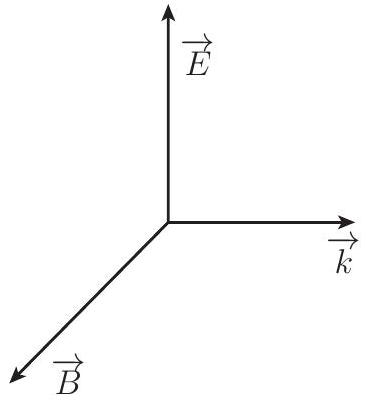
\includegraphics[width=0.7\textwidth]{images/propagation/prop-005-000.png}
\caption{Structure d'une onde plane progressive.}
\end{figure}

\begin{figure}[H]
\centering
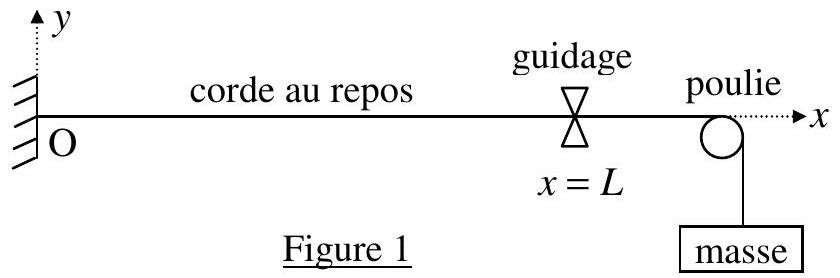
\includegraphics[width=0.7\textwidth]{images/propagation/prop-006-001.png}
\caption{Équation de propagation : schéma.}
\end{figure}

\begin{figure}[H]
\centering
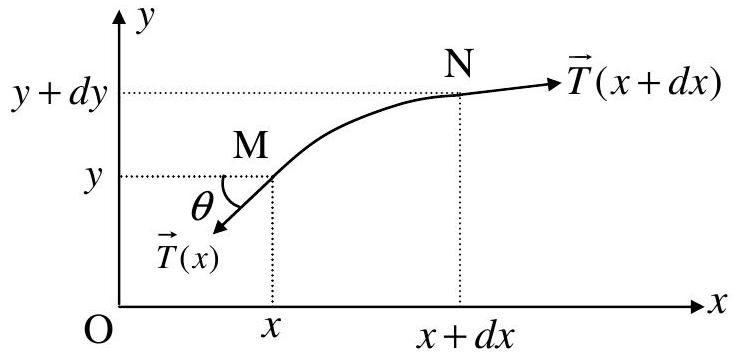
\includegraphics[width=0.7\textwidth]{images/propagation/prop-007-002.png}
\caption{Bilan énergétique d'une onde EM.}
\end{figure}

\begin{figure}[H]
\centering
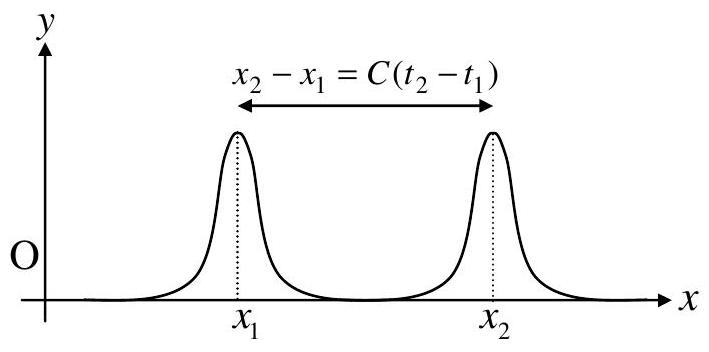
\includegraphics[width=0.7\textwidth]{images/propagation/prop-017-003.png}
\caption{Réflexion et transmission à une interface.}
\end{figure}

\begin{figure}[H]
\centering
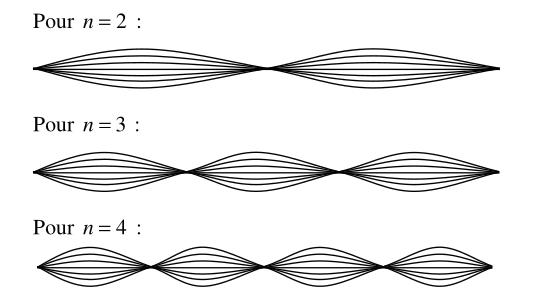
\includegraphics[width=0.7\textwidth]{images/propagation/prop-017-004.png}
\caption{Coefficients de Fresnel en incidence oblique.}
\end{figure}

\begin{figure}[H]
\centering
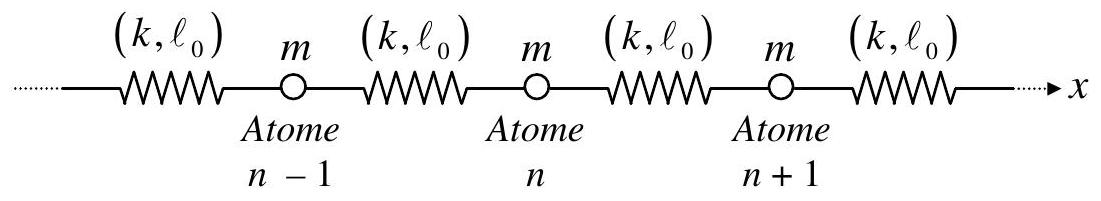
\includegraphics[width=0.7\textwidth]{images/propagation/prop-019-005.png}
\caption{Modes propres dans un milieu limité.}
\end{figure}

\begin{figure}[H]
\centering
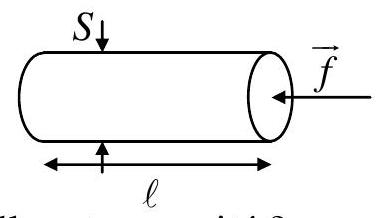
\includegraphics[width=0.7\textwidth]{images/propagation/prop-019-006.png}
\caption{Modes TE et TM dans un guide d'onde.}
\end{figure}

\begin{figure}[H]
\centering
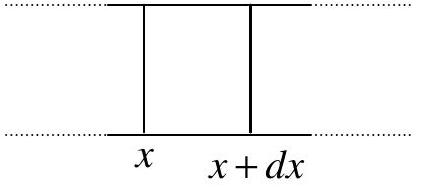
\includegraphics[width=0.7\textwidth]{images/propagation/prop-020-007.png}
\caption{Ligne de transmission : équations du télégraphiste.}
\end{figure}

\begin{figure}[H]
\centering
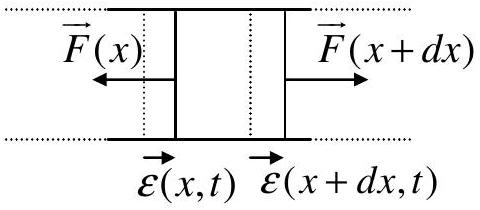
\includegraphics[width=0.7\textwidth]{images/propagation/prop-020-008.png}
\caption{Plasma : relation de dispersion.}
\end{figure}

\ifdefined\inMainDoc\else\end{document}\fi


% ================================================================
%  UE 13 : VIBRATIONS MÉCANIQUES
% ================================================================
\newpage
\thispagestyle{empty}
\begin{tikzpicture}[remember picture, overlay]
  \fill[gray!12] ([xshift=1.5cm, yshift=3cm]current page.south west)
    rectangle ([xshift=-1.5cm, yshift=-3cm]current page.north east);
  \draw[line width=3pt] ([xshift=1.5cm,yshift=-3cm]current page.north west)
    -- ([xshift=-1.5cm,yshift=-3cm]current page.north east);
  \draw[line width=3pt] ([xshift=1.5cm,yshift=3cm]current page.south west)
    -- ([xshift=-1.5cm,yshift=3cm]current page.south east);
  \node[align=center] at (current page.center) {%
    {\fontsize{30}{38}\bfseries\selectfont VIBRATIONS MÉCANIQUES}\\[1.2cm]
    {\large\itshape Oscillateurs libres et amortis}\\[0.4cm]
    {\large\itshape Résonance - Systèmes couplés}\\[1.8cm]
    {\normalsize Licence 3 - UE 13}
  };
  \node[anchor=south west] at ([xshift=2cm,yshift=2cm]current page.south west)
    {\large\bfseries UE 13};
\end{tikzpicture}
\newpage

\addcontentsline{toc}{section}{VIBRATIONS MÉCANIQUES}
\ifdefined\inMainDoc\else
\documentclass[12pt,a4paper]{article}
% ================================================================
%  PRÉAMBULE COMMUN - ANNALES CORRIGÉES
%  Université de Kara - FaST - Licence Fondamentale MPC
%  Design optimisé impression noir et blanc
% ================================================================

% -- ENCODAGE & LANGUE --
\usepackage[utf8]{inputenc}
\usepackage[T1]{fontenc}
\usepackage[french]{babel}
\usepackage{lmodern}
\usepackage{microtype}

% -- MISE EN PAGE --
\usepackage[a4paper, top=2.8cm, bottom=2.5cm, left=2.5cm, right=2.5cm, headheight=14pt]{geometry}
\usepackage{setspace}
\setstretch{1.2}
\usepackage{parskip}
\setlength{\parindent}{1.2em}
\setlength{\parskip}{4pt}

% -- MATHS --
\usepackage{amsmath, amssymb, mathtools, amsthm}
\usepackage{mathrsfs}
\usepackage{dsfont}
\usepackage{bm}
\usepackage{cancel}
\usepackage{textcomp}
% Définition de \oiint (intégrale de surface fermée) sans package supplémentaire
\newcommand{\oiint}{\mathop{\iint\!\!\!\!\!\!\!\bigcirc}\limits}

% -- PHYSIQUE & CHIMIE --
\usepackage{physics}
\usepackage{siunitx}
% Lorsque physics est chargé, siunitx omet \qty. On le restaure ici :
\AtBeginDocument{\RenewCommandCopy\qty\SI}
\sisetup{locale = FR, detect-all, output-decimal-marker={,}}
% Commande de substitution pour les unités posant problème avec pdflatex
% (ohm, degreeCelsius, micro, angstrom, percent utilisent des caractères non-ASCII)
\newcommand{\qtyohm}[1]{\ensuremath{\num{#1}\,\Omega}}
\newcommand{\qtydegc}[1]{\ensuremath{\num{#1}\,{}^\circ\text{C}}}
\newcommand{\qtyangstrom}[1]{\ensuremath{\num{#1}\,\text{\AA}}}
\newcommand{\qtypercent}[1]{\ensuremath{\num{#1}\,\%}}
\newcommand{\qtyum}[1]{\ensuremath{\num{#1}\,\mu\text{m}}}
\usepackage[version=4]{mhchem}

% -- GRAPHISMES --
\usepackage{graphicx}
\usepackage{float}
\usepackage{caption}
\usepackage{subcaption}
\usepackage{wrapfig}
\usepackage{tikz}
\usetikzlibrary{calc, arrows.meta, patterns, shapes.geometric}
\usepackage{pgfplots}
\pgfplotsset{compat=1.18}

% -- TABLEAUX --
\usepackage{booktabs}
\usepackage{array}
\usepackage{tabularx}
\usepackage{multirow}

% -- LISTES --
\usepackage{enumitem}
\setlist[enumerate]{topsep=3pt, itemsep=2pt, parsep=0pt}
\setlist[itemize]{topsep=3pt, itemsep=2pt, parsep=0pt, label={.}}

% -- BOÎTES (noir et blanc) --
\usepackage{mdframed}
\usepackage{tcolorbox}
\tcbuselibrary{skins, breakable, theorems}

% Boîte EXERCICE : encadré avec filet épais, fond blanc
\newmdenv[
  linewidth=1.2pt,
  linecolor=black,
  roundcorner=3pt,
  skipabove=10pt,
  skipbelow=6pt,
  innertopmargin=8pt,
  innerbottommargin=8pt,
  innerleftmargin=10pt,
  innerrightmargin=10pt,
  backgroundcolor=white,
  frametitle={\bfseries\small Exercice},
  frametitlealignment=\raggedright,
  frametitleaboveskip=4pt,
  frametitlebelowskip=4pt,
]{boiteexercice}

% Boîte CORRIGÉ : fond gris très clair + filet fin
\newmdenv[
  linewidth=0.6pt,
  linecolor=black,
  leftline=true,
  rightline=false,
  topline=false,
  bottomline=false,
  linecolor=black,
  innerleftmargin=12pt,
  innerrightmargin=8pt,
  innertopmargin=6pt,
  innerbottommargin=6pt,
  backgroundcolor=gray!8,
  skipabove=4pt,
  skipbelow=8pt,
]{boitecorrige}

% Boîte RÉSUMÉ DE COURS : double encadré
\newmdenv[
  linewidth=0.8pt,
  linecolor=black,
  roundcorner=2pt,
  backgroundcolor=gray!12,
  innertopmargin=10pt,
  innerbottommargin=10pt,
  innerleftmargin=12pt,
  innerrightmargin=12pt,
  skipabove=12pt,
  skipbelow=8pt,
]{boiteresume}

% Boîte ATTENTION/REMARQUE : barre gauche épaisse
\newmdenv[
  leftline=true,
  rightline=false,
  topline=false,
  bottomline=false,
  linewidth=3pt,
  linecolor=black,
  backgroundcolor=gray!5,
  innerleftmargin=12pt,
  innerrightmargin=8pt,
  innertopmargin=5pt,
  innerbottommargin=5pt,
  skipabove=6pt,
  skipbelow=6pt,
]{boiteremarque}

% -- DIFFICULTÉ DES EXERCICES --
\newcommand{\facile}{$\star$}
\newcommand{\moyen}{$\star\!\star$}
\newcommand{\difficile}{$\star\!\star\!\star$}
\newcommand{\niveau}[1]{\hfill\textbf{#1}\hspace{2pt}}

% -- EN-TÊTES ET PIEDS DE PAGE --
\usepackage{fancyhdr}
\pagestyle{fancy}
\fancyhf{}
\renewcommand{\headrulewidth}{0.5pt}
\renewcommand{\footrulewidth}{0.3pt}

% -- HYPERLIENS --
\usepackage[hidelinks]{hyperref}
\hypersetup{
    colorlinks=false,
    pdftitle={Annale Corrigée - Licence MPC - Université de Kara}
}

% -- TITRES --
\usepackage{titlesec}
\titleformat{\section}{\Large\bfseries}{\thesection.}{0.8em}{}[\vspace{2pt}\hrule\vspace{4pt}]
\titleformat{\subsection}{\large\bfseries}{\thesubsection.}{0.7em}{}
\titleformat{\subsubsection}{\normalsize\bfseries}{\thesubsubsection.}{0.6em}{}

% -- THÉORÈMES --
\theoremstyle{definition}
\newtheorem{defn}{Définition}[section]
\newtheorem{prop}{Propriété}[section]
\newtheorem{thm}{Théorème}[section]
\newtheorem{corol}{Corollaire}[section]
\newtheorem{exemple}{Exemple}[section]

% -- COMMANDES MATHÉMATIQUES UTILES --
\newcommand{\vect}[1]{\overrightarrow{#1}}
\newcommand{\R}{\mathbb{R}}
\newcommand{\N}{\mathbb{N}}
\newcommand{\Z}{\mathbb{Z}}
\newcommand{\C}{\mathbb{C}}
\renewcommand{\d}{\mathrm{d}}
\newcommand{\deriv}[2]{\dfrac{\d #1}{\d #2}}
\newcommand{\dpart}[2]{\dfrac{\partial #1}{\partial #2}}
\newcommand{\rot}{\overrightarrow{\mathrm{rot}}\,}
\renewcommand{\div}{\mathrm{div}\,}
\renewcommand{\grad}{\overrightarrow{\mathrm{grad}}\,}
\newcommand{\e}{\mathrm{e}}
\newcommand{\ii}{\mathrm{i}}
\renewcommand{\Tr}{\mathrm{Tr}}

% Numérotation des équations par section
\numberwithin{equation}{section}

% -- RÉSULTATS ENCADRÉS --
\newcommand{\res}[1]{\[\boxed{#1}\]}

% -- REMARQUE INLINE --
\newcommand{\rmq}[1]{\begin{boiteremarque}\textbf{Remarque.} #1\end{boiteremarque}}

% -- MISE EN VALEUR DU RÉSULTAT FINAL --
\newcommand{\reponse}[1]{%
  \begin{center}
    \fbox{\begin{minipage}{0.92\textwidth}\centering #1\end{minipage}}
  \end{center}%
}


\lhead{\small\textit{Vibrations Mécaniques - Licence 3}}
\rhead{\small\textit{FaST, Université de Kara}}
\cfoot{\thepage}

\begin{document}
\fi

\begin{center}
  {\LARGE\bfseries VIBRATIONS MÉCANIQUES}\\[0.3cm]
  {\normalsize Licence 3 - Physique}\\[0.1cm]
  \rule{0.7\textwidth}{0.8pt}
\end{center}

\section*{Résumé du cours}

\begin{boiteresume}

\textbf{1. Oscillateur harmonique libre.} Équation : $m\ddot{x} + kx = 0$. Pulsation propre $\omega_0 = \sqrt{k/m}$. Solution générale : $x(t) = A\cos(\omega_0 t + \varphi)$. Énergie : $E = \frac{1}{2}kA^2$ (constante).

\textbf{2. Formalisme de Lagrange.} $L = T - U$. Équation de Lagrange : $\frac{\mathrm{d}}{\mathrm{d}t}\!\left(\frac{\partial L}{\partial\dot{q}}\right) - \frac{\partial L}{\partial q} = Q$ où $Q$ est la force généralisée. Permet de traiter des systèmes complexes (poulies, disques) avec coordonnées généralisées naturelles.

\textbf{3. Oscillateur amorti.} Équation : $m\ddot{x} + f\dot{x} + kx = 0$ avec $f$ coefficient d'amortissement. Facteur de qualité $Q_f = m\omega_0/f$. Trois régimes : sous-amorti ($Q_f > 1/2$) $x=A\e^{-\omega_0 t/(2Q_f)}\cos(\omega_1 t+\varphi)$ avec $\omega_1=\omega_0\sqrt{1-1/(4Q_f^2)}$ ; critique ($Q_f=1/2$) ; sur-amorti ($Q_f < 1/2$).

\textbf{4. Oscillateur forcé.} Forçage $F_0\cos(\omega t)$. Amplitude en régime permanent : $A(\omega) = \frac{F_0/m}{\sqrt{(\omega_0^2-\omega^2)^2+(\omega\omega_0/Q_f)^2}}$. Résonance en amplitude à $\omega_r = \omega_0\sqrt{1-1/(2Q_f^2)}$ (sous-amorti). Résonance en vitesse à $\omega = \omega_0$.

\textbf{5. Systèmes à $n$ degrés de liberté.} Pour $n=2$, les pulsations propres sont solutions de $\det(K - \omega^2 M) = 0$ (problème aux valeurs propres). Les vecteurs propres donnent les modes normaux (formes modales).

\end{boiteresume}

\newpage
\section{Oscillations libres non amorties}

\subsection*{Exercice 1 - Barre avec masses et ressorts \niveau{\facile}}

\begin{boiteexercice}
Une barre de masse négligeable et de longueur $2\ell$ peut pivoter sans frottement autour de son milieu O. Aux extrémités sont fixées des masses $m_1$ et $m_2$. Trois ressorts de raideurs $k_1$, $k_2$ et $k_3$ rappellent la barre vers sa position d'équilibre horizontale ($\theta = 0$).
\begin{enumerate}
  \item En utilisant le formalisme de Lagrange avec la coordonnée généralisée $\theta$ (angle d'inclinaison), établir l'équation du mouvement pour de petites oscillations.
  \item Identifier la pulsation propre $\omega_0$.
  \item Écrire la solution $\theta(t)$ si $\theta(0) = \theta_0$ et $\dot{\theta}(0) = 0$.
\end{enumerate}
\end{boiteexercice}

\begin{boitecorrige}
\textbf{1.} Pour de petites oscillations ($\sin\theta\approx\theta$, $\cos\theta\approx 1$) :

Énergie cinétique : $T = \frac{1}{2}(m_1+m_2)\ell^2\dot\theta^2 = \frac{1}{2}m\ell^2\dot\theta^2$ avec $m=m_1+m_2$.

Énergie potentielle élastique (déplacement de chaque ressort $\approx \ell\theta$) :
$U = \frac{1}{2}(k_1+k_2+k_3)(\ell\theta)^2 = \frac{1}{2}k\ell^2\theta^2$ avec $k = k_1+k_2+k_3$.

Lagrangien : $L = T-U = \frac{1}{2}m\ell^2\dot\theta^2 - \frac{1}{2}k\ell^2\theta^2$.

Équation de Lagrange ($\partial L/\partial\dot\theta = m\ell^2\dot\theta$, $\partial L/\partial\theta = -k\ell^2\theta$) :
\[
m\ell^2\ddot\theta + k\ell^2\theta = 0 \quad\Longrightarrow\quad \ddot\theta + \frac{k}{m}\theta = 0
\]

\textbf{2.} Pulsation propre :
\[
\omega_0 = \sqrt{\frac{k}{m}} = \sqrt{\frac{k_1+k_2+k_3}{m_1+m_2}}
\]

\textbf{3.} Système libre non amorti avec $\theta(0)=\theta_0$, $\dot\theta(0)=0$ :
\[
\theta(t) = \theta_0\cos(\omega_0 t)
\]
\end{boitecorrige}

\subsection*{Exercice 2 - Poulie avec ressort et masse \niveau{\moyen}}

\begin{boiteexercice}
Une poulie homogène de masse $M$, de rayon $R$ et de moment d'inertie $J_O = MR^2/2$ peut tourner sans frottement autour de son axe fixe O. Un ressort de raideur $k$ est accroché à la poulie, et un corps de masse $m$ est suspendu par un fil inextensible enroulé sur la poulie. On note $\theta$ la rotation de la poulie ($x = R\theta$ le déplacement vertical de $m$).
\begin{enumerate}
  \item Écrire le lagrangien $L$ du système.
  \item Établir l'équation du mouvement.
  \item Calculer la pulsation propre $\omega_0$.
\end{enumerate}
\end{boiteexercice}

\begin{boitecorrige}
\textbf{1.} Énergie cinétique totale (poulie + masse) :
\[
T = \frac{1}{2}J_O\dot\theta^2 + \frac{1}{2}m\dot x^2 = \frac{1}{2}\cdot\frac{MR^2}{2}\dot\theta^2 + \frac{1}{2}mR^2\dot\theta^2 = \frac{1}{2}\!\left(\frac{M}{2}+m\right)R^2\dot\theta^2
\]
Énergie potentielle (ressort comprimé de $R\theta$, on choisit le repère tel que l'énergie gravitationnelle soit incluse dans la position d'équilibre) :
\[
U = \frac{1}{2}k(R\theta)^2
\]
Lagrangien :
\[
L = \frac{1}{2}\!\left(\frac{M}{2}+m\right)R^2\dot\theta^2 - \frac{1}{2}kR^2\theta^2
\]

\textbf{2.} Équation de Lagrange :
\[
\left(\frac{M}{2}+m\right)R^2\ddot\theta + kR^2\theta = 0 \quad\Longrightarrow\quad \left(\frac{M}{2}+m\right)\ddot\theta + k\theta = 0
\]

\textbf{3.} Pulsation propre :
\[
\omega_0 = \sqrt{\frac{2k}{M+2m}}
\]
\end{boitecorrige}

\section{Oscillations amorties et forcées}

\subsection*{Exercice 3 - Oscillateur amorti \niveau{\moyen}}

\begin{boiteexercice}
Un oscillateur masse-ressort-amortisseur est caractérisé par $m = \qty{0.5}{kg}$, $k = \qty{50}{N.m^{-1}}$ et $f = \qty{2}{kg.s^{-1}}$ (coefficient d'amortissement visqueux).
\begin{enumerate}
  \item Calculer la pulsation propre $\omega_0$, la pulsation d'amortissement $\lambda = f/(2m)$ et le facteur de qualité $Q_f$.
  \item Déterminer le régime (sous-amorti, critique, sur-amorti).
  \item Écrire la solution générale $x(t)$.
  \item Calculer le décrément logarithmique $\delta = \pi/(Q_f\sqrt{1-1/(4Q_f^2)})$.
  \item Au bout de combien d'oscillations l'amplitude est-elle réduite à 1\% de sa valeur initiale ?
\end{enumerate}
\end{boiteexercice}

\begin{boitecorrige}
\textbf{1.} $\omega_0 = \sqrt{k/m} = \sqrt{50/0{,}5} = \qty{10}{rad.s^{-1}}$. $\lambda = f/(2m) = 2/(2\times0{,}5) = \qty{2}{s^{-1}}$.
$Q_f = m\omega_0/f = 0{,}5\times10/2 = 2{,}5$.

\textbf{2.} $Q_f = 2{,}5 > 1/2$ : régime \textbf{sous-amorti}.

\textbf{3.} Pulsation des oscillations amorties :
\[
\omega_1 = \omega_0\sqrt{1-\frac{1}{4Q_f^2}} = 10\sqrt{1-\frac{1}{25}} = 10\sqrt{0{,}96} \approx \qty{9.80}{rad.s^{-1}}
\]
Solution générale :
\[
x(t) = A\e^{-\lambda t}\cos(\omega_1 t+\varphi) = A\e^{-2t}\cos(9{,}80\,t+\varphi)
\]

\textbf{4.} Décrément logarithmique $\delta = \ln(x_n/x_{n+1}) = \lambda T_1$ avec $T_1 = 2\pi/\omega_1$ :
\[
\delta = \lambda\cdot\frac{2\pi}{\omega_1} = \frac{2\times2\pi}{9{,}80} \approx 1{,}28
\]

\textbf{5.} Après $N$ oscillations, l'amplitude est $A_N = A_0\e^{-N\delta}$. On cherche $N$ tel que $A_N = 0{,}01\,A_0$ :
\[
N = \frac{\ln(100)}{\delta} = \frac{4{,}61}{1{,}28} \approx 3{,}6
\]
Il faut donc environ 4 oscillations pour que l'amplitude soit inférieure à 1\% de $A_0$.
\end{boitecorrige}

\subsection*{Exercice 4 - Résonance d'un oscillateur forcé \niveau{\difficile}}

\begin{boiteexercice}
L'oscillateur de l'exercice 3 est soumis à une force $F(t) = F_0\cos(\omega t)$ avec $F_0 = \qty{5}{N}$.
\begin{enumerate}
  \item Écrire l'équation du mouvement.
  \item Donner l'amplitude $A(\omega)$ de l'oscillation en régime permanent.
  \item Calculer $A(\omega_0)$ (amplitude à la pulsation propre).
  \item Calculer $\omega_r$ (pulsation de résonance en amplitude) et $A_{\max} = A(\omega_r)$.
  \item Représenter qualitativement $A(\omega)$ et indiquer la largeur de la résonance $\Delta\omega = \omega_0/Q_f$.
\end{enumerate}
\end{boiteexercice}

\begin{boitecorrige}
\textbf{1.} Équation du mouvement :
\[
m\ddot x + f\dot x + kx = F_0\cos(\omega t) \quad\Longrightarrow\quad \ddot x + 2\lambda\dot x + \omega_0^2 x = \frac{F_0}{m}\cos(\omega t)
\]

\textbf{2.} Amplitude en régime permanent :
\[
A(\omega) = \frac{F_0/m}{\sqrt{(\omega_0^2-\omega^2)^2 + 4\lambda^2\omega^2}}
\]
Amplitude statique : $A_{stat} = F_0/k = 5/50 = \qty{0.1}{m}$.

\textbf{3.} À $\omega = \omega_0$ :
\[
A(\omega_0) = \frac{F_0/m}{2\lambda\omega_0} = \frac{F_0}{f\omega_0} = \frac{5}{2\times10} = \qty{0.25}{m} = Q_f\times A_{stat}
\]
L'amplitude à la pulsation propre vaut $Q_f$ fois l'amplitude statique.

\textbf{4.} Pulsation de résonance en amplitude :
\[
\omega_r = \omega_0\sqrt{1-\frac{1}{2Q_f^2}} = 10\sqrt{1-\frac{1}{12{,}5}} = 10\sqrt{0{,}92} \approx \qty{9.59}{rad.s^{-1}}
\]
Amplitude maximale :
\[
A_{\max} = \frac{F_0/m}{\omega_0^2}\cdot\frac{Q_f}{\sqrt{1-1/(4Q_f^2)}} \approx A_{stat}Q_f\left(1+\frac{1}{8Q_f^2}\right) \approx \qty{0.252}{m}
\]

\textbf{5.} La courbe $A(\omega)$ présente un pic de largeur $\Delta\omega = \omega_0/Q_f = 10/2{,}5 = \qty{4}{rad.s^{-1}}$ à mi-hauteur (en puissance). Plus $Q_f$ est grand, plus le pic est étroit et la résonance sélective.
\end{boitecorrige}

\section{Systèmes couplés}

\subsection*{Exercice 5 - Deux masses couplées \niveau{\difficile}}

\begin{boiteexercice}
Deux masses $m$ sont reliées entre elles par un ressort de raideur $k$ et chacune est reliée à un support fixe par un ressort de raideur $K$. Les déplacements sont $x_1$ et $x_2$.
\begin{enumerate}
  \item Écrire les équations du mouvement couplées.
  \item Chercher des solutions de la forme $x_1 = A_1\e^{\ii\omega t}$, $x_2 = A_2\e^{\ii\omega t}$ et écrire le système matriciel.
  \item Calculer les deux pulsations propres $\omega_1$ et $\omega_2$.
  \item Décrire les deux modes normaux (formes modales).
  \item Si $K=k$, calculer $\omega_1$ et $\omega_2$ numériquement pour $m=\qty{1}{kg}$, $k=\qty{4}{N.m^{-1}}$.
\end{enumerate}
\end{boiteexercice}

\begin{boitecorrige}
\textbf{1.} Équations du mouvement (ressort central déformé de $x_2-x_1$) :
\[
\begin{cases}
m\ddot x_1 = -Kx_1 + k(x_2-x_1) = -(K+k)x_1 + kx_2\\
m\ddot x_2 = -Kx_2 - k(x_2-x_1) = kx_1 - (K+k)x_2
\end{cases}
\]

\textbf{2.} En substituant $x_i = A_i\e^{\ii\omega t}$ (donc $\ddot x_i = -\omega^2 A_i\e^{\ii\omega t}$) :
\[
\begin{pmatrix}K+k-m\omega^2 & -k\\ -k & K+k-m\omega^2\end{pmatrix}\begin{pmatrix}A_1\\A_2\end{pmatrix} = \begin{pmatrix}0\\0\end{pmatrix}
\]

\textbf{3.} Pour avoir une solution non triviale, le déterminant doit être nul :
\[
(K+k-m\omega^2)^2 - k^2 = 0 \quad\Longrightarrow\quad K+k-m\omega^2 = \pm k
\]
\[
\omega_1^2 = \frac{K}{m}, \qquad \omega_2^2 = \frac{K+2k}{m}
\]

\textbf{4.} Mode 1 ($\omega_1^2 = K/m$) : $(K+k-m\omega_1^2)A_1 = kA_2$, soit $kA_1 = kA_2$ donc $A_1 = A_2$. Les deux masses oscillent \textbf{en phase} avec la même amplitude : le ressort central ne se déforme pas. Mode 2 ($\omega_2^2 = (K+2k)/m$) : $A_1 = -A_2$. Les deux masses oscillent en \textbf{opposition de phase} : le milieu du ressort central est un n\oe{}ud fixe.

\textbf{5.} Pour $K=k=\qty{4}{N.m^{-1}}$, $m=\qty{1}{kg}$ :
\[
\omega_1 = \sqrt{K/m} = \sqrt{4} = \qty{2}{rad.s^{-1}}, \qquad \omega_2 = \sqrt{3K/m} = \sqrt{12} \approx \qty{3.46}{rad.s^{-1}}
\]
\end{boitecorrige}


\section{Oscillations amorties}

\subsection*{Exercice 6 - Barre oscillante avec amortissement \niveau{\moyen}}

\begin{boiteexercice}
Soit un système mécanique vibratoire constitué d'une barre de masse $M$ et de longueur $L$, articulée en $O$. Si $G$ est le centre de gravité de la barre ($J_{/G} = \frac{1}{12}ML^2$, $OA = L_1$, $OB = L_2$).
\begin{enumerate}
  \item Trouver l'équation différentielle du mouvement pour de faibles oscillations. Déduire $\delta$ et $\omega_0$.
  \item Écrire la solution dans le cas $\delta < \omega_0$.
\end{enumerate}
En chaque extrémité, des ressorts de raideur $k$ et des amortisseurs de coefficient $\alpha$ sont fixés aux points $A$ et $B$.
\end{boiteexercice}

\begin{boitecorrige}
\textbf{1.} On calcule le moment d'inertie par rapport à $O$ (Huygens) :
\[
J_{/O} = J_{/G} + M\!\left(\frac{L}{2}\right)^2 = \frac{1}{12}ML^2 + \frac{1}{4}ML^2 = \frac{1}{3}ML^2
\]
L'énergie cinétique : $T = \frac{1}{2}J_{/O}\dot\theta^2$. L'énergie potentielle (ressorts) :
\[
U = \frac{1}{2}k(L_1\sin\theta)^2 + \frac{1}{2}k(L_2\sin\theta)^2 \approx \frac{k(L_1^2+L_2^2)}{2}\theta^2
\]
La fonction de dissipation : $D = \frac{1}{2}\alpha(L_1\dot\theta)^2 + \frac{1}{2}\alpha(L_2\dot\theta)^2 = \frac{\alpha(L_1^2+L_2^2)}{2}\dot\theta^2$.

L'équation de Lagrange avec dissipation donne :
\[
\frac{1}{3}ML^2\ddot\theta + \alpha(L_1^2+L_2^2)\dot\theta + k(L_1^2+L_2^2)\theta = 0
\]
soit $\ddot\theta + 2\delta\dot\theta + \omega_0^2\theta = 0$ avec :
\[
2\delta = \frac{\alpha(L_1^2+L_2^2)}{\frac{1}{3}ML^2}, \qquad \omega_0^2 = \frac{k(L_1^2+L_2^2)}{\frac{1}{3}ML^2}
\]

\textbf{2.} Pour $\delta < \omega_0$ (régime sous-amorti), la solution est :
\[
\theta(t) = C\,\e^{-\delta t}\sin(\omega_a t + \varphi), \qquad \omega_a = \sqrt{\omega_0^2 - \delta^2}
\]
\end{boitecorrige}

\section{Oscillations forcées}

\subsection*{Exercice 7 - Oscillateur forcé avec amortisseur \niveau{\moyen}}

\begin{boiteexercice}
Une masse $m$, suspendue par un ressort de raideur $k$ et un amortisseur de coefficient $\alpha$, oscille verticalement sous l'effet d'une excitation $F(t) = F_0\cos(\Omega t)$.
\begin{enumerate}
  \item Écrire l'énergie cinétique $T$, l'énergie potentielle $U$ et la fonction de dissipation $D$.
  \item Établir l'équation du mouvement par le formalisme de Lagrange.
  \item À l'aide de la représentation complexe, trouver la solution permanente (amplitude $A$ et phase $\phi$).
  \item Donner la condition de résonance et la pulsation de résonance $\Omega_R$.
  \item Donner la bande passante $B$ pour un amortissement faible $\lambda \ll \omega_0$.
\end{enumerate}
\end{boiteexercice}

\begin{boitecorrige}
\textbf{1.} $T = \frac{1}{2}m\dot{y}^2$, $U = \frac{1}{2}ky^2$ (condition d'équilibre déduite), $D = \frac{1}{2}\alpha\dot{y}^2$.

\textbf{2.} L'équation de Lagrange avec dissipation et force extérieure donne :
\[
m\ddot{y} + \alpha\dot{y} + ky = F_0\cos\Omega t \quad\Longrightarrow\quad \ddot{y} + 2\lambda\dot{y} + \omega_0^2 y = \frac{F_0}{m}\cos\Omega t
\]
avec $\lambda = \dfrac{\alpha}{2m}$ et $\omega_0^2 = \dfrac{k}{m}$.

\textbf{3.} En posant $y_c = \underline{A}\,\e^{j\Omega t}$ :
\[
(-\Omega^2 + 2\lambda j\Omega + \omega_0^2)\underline{A} = \frac{F_0}{m} \implies \underline{A} = \frac{F_0/m}{\omega_0^2 - \Omega^2 + 2\lambda j\Omega}
\]
\[
A = \frac{F_0/m}{\sqrt{(\omega_0^2-\Omega^2)^2 + 4\lambda^2\Omega^2}}, \qquad \tan\phi = \frac{-2\lambda\Omega}{\omega_0^2-\Omega^2}
\]

\textbf{4.} En annulant $\partial A/\partial\Omega = 0$ :
\[
\Omega_R = \sqrt{\omega_0^2 - 2\lambda^2}
\]

\textbf{5.} Pour $\lambda \ll \omega_0$ : $\Omega_{c_1} \approx \omega_0 - \lambda$, $\Omega_{c_2} \approx \omega_0 + \lambda$, donc $B = 2\lambda$.
\end{boitecorrige}

\subsection*{Exercice 8 - Pendule forcé sur tige \niveau{\difficile}}

\begin{boiteexercice}
Une boule ponctuelle de masse $m$ est fixée à l'extrémité d'une tige de longueur $3\ell$ (masse négligeable). Au point situé à $2\ell$ de $O$, un amortisseur de coefficient $\alpha$ est attaché. L'extrémité de la tige porte une force $F(t) = F_0\cos(\Omega t)$.
\begin{enumerate}
  \item Trouver $T$, $U$ et $D$ pour $\theta \ll 1$.
  \item Établir l'équation du mouvement par Lagrange.
  \item Trouver la solution permanente (amplitude et phase).
  \item Déduire la pulsation de résonance $\Omega_R$.
  \item Donner $\Omega_{c1}$, $\Omega_{c2}$ et $B$ pour $\lambda \ll \omega_0$.
  \item Calculer numériquement $\Omega_R$, $B$ et le facteur de qualité $Q$ pour $m=1$\,kg, $k=15$\,N/m, $\ell=0{,}5$\,m, $\alpha=0{,}5$\,N$\cdot$s/m, $g=10$\,m/s$^2$.
\end{enumerate}
\end{boiteexercice}

\begin{boitecorrige}
\textbf{1.} Pour $\theta\ll1$ : $T = \frac{9}{2}m\ell^2\dot\theta^2$, $U \approx \frac{1}{2}(3mg\ell + k\ell^2)\theta^2$, $D = 2\alpha\ell^2\dot\theta^2$.

\textbf{2.} L'équation de Lagrange donne :
\[
9m\ell^2\ddot\theta + 4\alpha\ell^2\dot\theta + (3mg\ell + k\ell^2)\theta = 3\ell F_0\cos\Omega t
\]
\[
\ddot\theta + \frac{4\alpha}{9m}\dot\theta + \left(\frac{g}{3\ell}+\frac{k}{9m}\right)\theta = \frac{F_0}{3m\ell}\cos\Omega t
\]
avec $\lambda = \dfrac{2\alpha}{9m}$ et $\omega_0^2 = \dfrac{g}{3\ell}+\dfrac{k}{9m}$.

\textbf{3.}
\[
A = \frac{F_0/(3m\ell)}{\sqrt{(\omega_0^2-\Omega^2)^2+4\lambda^2\Omega^2}}, \qquad \tan\phi = \frac{-2\lambda\Omega}{\omega_0^2-\Omega^2}
\]

\textbf{4.} $\Omega_R = \sqrt{\omega_0^2 - 2\lambda^2}$.

\textbf{5.} Pour $\lambda \ll \omega_0$ : $B = 2\lambda$.

\textbf{6.} Application numérique :
\[
\omega_0^2 = \frac{10}{1.5} + \frac{15}{9} \approx 8.33 \implies \omega_0 \approx 2.89\,\text{rad/s}
\]
\[
\lambda = \frac{2\times 0.5}{9\times 1} \approx 0.111\,\text{rad/s}, \quad \Omega_R \approx 2.88\,\text{rad/s}, \quad B \approx 0.222\,\text{rad/s}
\]
\[
Q = \frac{\omega_0}{2\lambda} \approx 13
\]
\end{boitecorrige}

\subsection*{Exercice 9 - Système poulie-masse forcé \niveau{\difficile}}

\begin{boiteexercice}
Un disque (masse $m_1$, rayon $R$) est suspendu par un ressort $k$ (au dessus) et porte une masse $m_2$ via un fil inextensible enroulé dessus. Un amortisseur $\alpha$ est fixé. Une force $F(t) = F_0\cos(\Omega t)$ est appliquée sur le fil.
\begin{enumerate}
  \item Écrire $T$, $U$ et $D$.
  \item Établir l'équation du mouvement.
  \item Trouver la solution permanente.
  \item Déduire $\Omega_R$.
  \item Donner $B$ pour $\lambda \ll \omega_0$.
  \item Calculer $\Omega_R$, $B$ et $Q$ pour $m_1=2$\,kg, $m_2=1$\,kg, $k=10$\,N/m, $\alpha=0{,}1$\,N$\cdot$s/m.
\end{enumerate}
\end{boiteexercice}

\begin{boitecorrige}
\textbf{1.} En notant $\theta$ la rotation du disque ($x = R\theta$) :
\[
T = \frac{1}{2}(m_1+m_2)R^2\dot\theta^2, \quad U = \frac{1}{2}kR^2\theta^2, \quad D = \frac{1}{2}\alpha R^2\dot\theta^2
\]
(les termes linéaires s'éliminent à l'équilibre).

\textbf{2.} L'équation du mouvement est :
\[
(m_1+m_2)\ddot\theta + \frac{\alpha}{m_1+m_2}\dot\theta\cdot(m_1+m_2) + k\theta = \frac{F_0}{(m_1+m_2)R}\cos\Omega t
\]
\[
\ddot\theta + \frac{\alpha}{m_1+m_2}\dot\theta + \frac{k}{m_1+m_2}\theta = \frac{F_0}{(m_1+m_2)R}\cos\Omega t
\]
avec $\lambda = \dfrac{\alpha}{2(m_1+m_2)}$ et $\omega_0^2 = \dfrac{k}{m_1+m_2}$.

\textbf{3.}
\[
A = \frac{F_0/[(m_1+m_2)R]}{\sqrt{(\omega_0^2-\Omega^2)^2+4\lambda^2\Omega^2}}, \qquad \tan\phi = \frac{-2\lambda\Omega}{\omega_0^2-\Omega^2}
\]

\textbf{4.} $\Omega_R = \sqrt{\omega_0^2 - 2\lambda^2}$.

\textbf{5.} $B = 2\lambda = \dfrac{\alpha}{m_1+m_2}$.

\textbf{6.} Pour $m_1=2$\,kg, $m_2=1$\,kg, $k=10$\,N/m, $\alpha=0{,}1$\,N$\cdot$s/m :
\[
\omega_0^2 = \frac{10}{3} \implies \omega_0 \approx 1.83\,\text{rad/s}
\]
\[
\lambda = \frac{0.1}{2\times3} \approx 0.0167\,\text{rad/s}, \quad \Omega_R \approx 1.83\,\text{rad/s}, \quad B \approx 0.033\,\text{rad/s}
\]
\[
Q = \frac{\omega_0}{2\lambda} \approx 54.8
\]
\end{boitecorrige}

\section{Systèmes à deux degrés de liberté}

\clearpage
\subsection*{Exercice 10 - Deux oscillateurs couplés \niveau{\difficile}}

\begin{boiteexercice}
Deux masses identiques $m$ sont reliées à des parois fixes par des ressorts de raideur $k$, et couplées entre elles par un ressort de raideur $k'$.
\begin{enumerate}
  \item Écrire le lagrangien et le mettre sous la forme $L = \frac{1}{2}m[(\dot x_1^2+\dot x_2^2) - \omega_0^2(x_1^2+x_2^2-2Cx_1x_2)]$.
  \item Donner $\omega_0^2$ et $C$ (coefficient de couplage) et écrire les équations du mouvement.
  \item Déterminer les pulsations propres.
  \item Trouver $x_1(t)$ et $x_2(t)$ pour $x_1(0)=x_0$, $\dot x_1(0)=0$, $x_2(0)=0$, $\dot x_2(0)=0$.
\end{enumerate}
\end{boiteexercice}

\begin{boitecorrige}
\textbf{1.} Le lagrangien est :
\[
L = \frac{1}{2}m\dot x_1^2 + \frac{1}{2}m\dot x_2^2 - \frac{1}{2}kx_1^2 - \frac{1}{2}k'(x_2-x_1)^2 - \frac{1}{2}kx_2^2
\]
En développant et regroupant :
\[
L = \frac{1}{2}m\left[(\dot x_1^2+\dot x_2^2) - \frac{k+k'}{m}\left(x_1^2+x_2^2-\frac{2k'}{k+k'}x_1x_2\right)\right]
\]

\textbf{2.} On identifie : $\omega_0^2 = \dfrac{k+k'}{m}$ et $C = \dfrac{k'}{k+k'}$. Les équations du mouvement sont :
\[
\ddot x_1 + \omega_0^2 x_1 = C\omega_0^2 x_2, \qquad \ddot x_2 + \omega_0^2 x_2 = C\omega_0^2 x_1
\]

\textbf{3.} En cherchant des solutions harmoniques $x_i = A_i\e^{j\omega t}$, la condition de non-trivialité donne :
\[
(\omega_0^2-\omega^2)^2 - (C\omega_0^2)^2 = 0 \implies \omega_{1,2} = \omega_0\sqrt{1 \mp C}
\]
Mode 1 ($\omega_1$) : $x_2 = x_1$ (en phase). Mode 2 ($\omega_2$) : $x_2 = -x_1$ (opposition de phase).

\textbf{4.} La solution générale est :
\[
\binom{x_1}{x_2} = A\binom{1}{1}\cos(\omega_1 t+\varphi_1) + B\binom{1}{-1}\cos(\omega_2 t+\varphi_2).
\]

Avec les conditions initiales : $\varphi_1=\varphi_2=0$, $A=B=x_0/2$, donc :
\[
x_1(t) = \tfrac{x_0}{2}(\cos\omega_1 t + \cos\omega_2 t), \quad x_2(t) = \tfrac{x_0}{2}(\cos\omega_1 t - \cos\omega_2 t)
\]
\end{boitecorrige}

\newpage

\subsection*{Exercice 11 - Deux oscillateurs couplés par amortisseur \niveau{\difficile}}

\begin{boiteexercice}
Deux oscillateurs verticaux ($m_1, k$) et ($m_2, k$) sont couplés par un amortisseur $\alpha$.
\begin{enumerate}
  \item Déterminer les équations différentielles du mouvement en fonction de $y_1(t)$ et $y_2(t)$.
  \item Pour $m_1 = m_2 = m$, introduire $Y_1 = y_1 - y_2$ et $Y_2 = y_1 + y_2$ et déduire deux équations différentielles indépendantes.
\end{enumerate}
\end{boiteexercice}

\begin{boitecorrige}
\textbf{1.} L'énergie cinétique : $T = \frac{1}{2}m_1\dot y_1^2 + \frac{1}{2}m_2\dot y_2^2$.
L'énergie potentielle : $U = \frac{1}{2}ky_1^2 + \frac{1}{2}ky_2^2$.
La fonction de dissipation : $D = \frac{1}{2}\alpha(\dot y_1-\dot y_2)^2$.

Le formalisme de Lagrange avec dissipation donne :
\[
\begin{cases}
m_1\ddot y_1 + \alpha\dot y_1 + ky_1 = \alpha\dot y_2 \\
m_2\ddot y_2 + \alpha\dot y_2 + ky_2 = \alpha\dot y_1
\end{cases}
\]

\textbf{2.} Pour $m_1=m_2=m$, on additionne et soustrait les deux équations :

Soustraction (1)$-$(2) :
\[
m(\ddot y_1-\ddot y_2) + 2\alpha(\dot y_1-\dot y_2) + k(y_1-y_2) = 0 \implies m\ddot Y_1 + 2\alpha\dot Y_1 + kY_1 = 0
\]

Addition (1)$+$(2) :
\[
m(\ddot y_1+\ddot y_2) + k(y_1+y_2) = 0 \implies m\ddot Y_2 + kY_2 = 0
\]

Les deux équations découplées sont :
\[
\ddot Y_1 + \frac{2\alpha}{m}\dot Y_1 + \frac{k}{m}Y_1 = 0 \quad\text{(amortie)}, \qquad \ddot Y_2 + \frac{k}{m}Y_2 = 0 \quad\text{(non amortie)}
\]
\end{boitecorrige}


\subsection*{Exercice 12 - Oscillateur forcé avec amortissement \niveau{\moyen}}

\begin{boiteexercice}
Un oscillateur de masse $m=0{,}5\;\text{kg}$, raideur $k=50\;\text{N/m}$ et coefficient d'amortissement $b=2\;\text{N\,s/m}$ est soumis à une force $F(t)=F_0\cos(\omega t)$ avec $F_0=10\;\text{N}$.
\begin{enumerate}
  \item Écrire l'équation différentielle du mouvement.
  \item Donner l'expression de l'amplitude $A(\omega)$ de la solution stationnaire $x(t)=A(\omega)\cos(\omega t-\varphi)$.
  \item Calculer $\omega_0$, le facteur de qualité $Q_f=m\omega_0/b$ et l'amplitude statique $A_0=F_0/k$.
  \item Déterminer la pulsation de résonance $\omega_\text{res}$ et l'amplitude maximale $A_\text{max}$.
  \item Tracer qualitativement $A(\omega)/A_0$ en fonction de $\omega/\omega_0$.
\end{enumerate}
\end{boiteexercice}

\begin{boitecorrige}
\textbf{1.} Le principe fondamental avec force de rappel, amortissement visqueux et force extérieure :
\[
m\ddot{x} + b\dot{x} + kx = F_0\cos(\omega t)
\]

\textbf{2.} En régime permanent, on cherche $x_p(t)=A\cos(\omega t-\varphi)$. En substituant et en identifiant :
\[
\boxed{A(\omega) = \frac{F_0/m}{\sqrt{(\omega_0^2-\omega^2)^2+(b\omega/m)^2}}}
\]
avec la phase $\varphi = \arctan\!\left(\dfrac{b\omega/m}{\omega_0^2-\omega^2}\right)$.

\textbf{3.} Les paramètres numériques :
\[
\omega_0 = \sqrt{\frac{k}{m}} = \sqrt{\frac{50}{0{,}5}} = \sqrt{100} = \qty{10}{rad/s}, \qquad Q_f = \frac{m\omega_0}{b} = \frac{0{,}5\times10}{2} = 2{,}5
\]
\[
A_0 = \frac{F_0}{k} = \frac{10}{50} = \qty{0.2}{m}
\]

\textbf{4.} L'amplitude est maximale lorsque le dénominateur est minimal. On minimise $f(\omega^2)=(\omega_0^2-\omega^2)^2+(b/m)^2\omega^2$ en dérivant par rapport à $\omega^2$ :
\[
\frac{d f}{d(\omega^2)} = -2(\omega_0^2-\omega^2) + \frac{b^2}{m^2} = 0 \implies \omega^2 = \omega_0^2 - \frac{b^2}{2m^2}
\]
\[
\omega_\text{res} = \sqrt{\omega_0^2 - \frac{b^2}{2m^2}} = \sqrt{100 - \frac{4}{2\times0{,}25}} = \sqrt{100-8} = \sqrt{92} \approx \qty{9.59}{rad/s}
\]
L'amplitude maximale :
\[
A_\text{max} = \frac{F_0/m}{\frac{b}{m}\omega_0\sqrt{1 - \frac{1}{4Q_f^2}}} = \frac{Q_f \,A_0}{\sqrt{1-\frac{1}{4Q_f^2}}} = \frac{2{,}5\times0{,}2}{\sqrt{1-0{,}04}} \approx \frac{0{,}5}{0{,}98} \approx \qty{0.51}{m}
\]

\textbf{5.} Pour $Q_f=2{,}5>1/\sqrt{2}$, il y a résonance. La courbe part de $A/A_0=1$ en $\omega=0$, présente un maximum voisin de $Q_f=2{,}5$ à $\omega\approx\omega_0$, puis décroît en $\omega^{-2}$ pour $\omega\gg\omega_0$.
\end{boitecorrige}

\subsection*{Exercice 13 - Ondes progressives sur une corde \niveau{\moyen}}

\begin{boiteexercice}
Une corde de longueur $L=2\;\text{m}$, masse linéique $\mu=10\;\text{g/m}$, est tendue avec une tension $T=40\;\text{N}$.
\begin{enumerate}
  \item Établir l'équation d'onde unidimensionnelle et identifier la célérité $c$.
  \item Calculer $c$ numériquement.
  \item La corde est excitée à $x=0$ par $y(0,t)=A\sin(\omega t)$ avec $A=5\;\text{mm}$ et $f=100\;\text{Hz}$. Écrire l'onde progressive $y(x,t)$ se propageant vers les $x>0$.
  \item Calculer la puissance moyenne transportée par l'onde.
  \item Exprimer les densités d'énergie cinétique et potentielle et montrer qu'elles sont égales en moyenne.
\end{enumerate}
\end{boiteexercice}

\begin{boitecorrige}
\textbf{1.} En appliquant le PFD à un élément $\text{d}x$ de corde (petits déplacements transverses) :
\[
\mu\,\text{d}x\,\frac{\partial^2 y}{\partial t^2} = T\,\text{d}x\,\frac{\partial^2 y}{\partial x^2} \implies \boxed{\frac{\partial^2 y}{\partial t^2} = c^2\,\frac{\partial^2 y}{\partial x^2}}, \quad c = \sqrt{\frac{T}{\mu}}
\]
La solution générale est $y(x,t)=f(x-ct)+g(x+ct)$ (d'Alembert).

\textbf{2.} Numériquement :
\[
c = \sqrt{\frac{T}{\mu}} = \sqrt{\frac{40}{0{,}010}} = \sqrt{4000} \approx \qty{63.2}{m/s}
\]

\textbf{3.} L'onde se propageant vers $+x$ :
\[
y(x,t) = A\sin\!\left(\omega t - \frac{\omega}{c}x\right) = A\sin(\omega t - kx)
\]
avec $k = \omega/c = 2\pi f/c = 2\pi\times100/63{,}2 \approx \qty{9.94}{rad/m}$ et $\lambda = c/f = 63{,}2/100 \approx \qty{0.632}{m}$.

\textbf{4.} La vitesse transverse est $v_y=\partial y/\partial t = A\omega\cos(\omega t-kx)$. La puissance instantanée $\mathcal{P} = -T\,(\partial y/\partial x)\,(\partial y/\partial t) = T k A^2\omega\cos^2(\omega t-kx)$. En moyenne :
\[
\langle\mathcal{P}\rangle = \frac{1}{2}TkA^2\omega = \frac{1}{2}\mu c\,\omega^2 A^2
\]
Numériquement : $\langle\mathcal{P}\rangle = \frac{1}{2}\times0{,}010\times63{,}2\times(2\pi\times100)^2\times(5\times10^{-3})^2 \approx \qty{4.93}{W}$.

\textbf{5.} Densité d'énergie cinétique : $e_c = \frac{1}{2}\mu(\partial y/\partial t)^2 = \frac{1}{2}\mu\omega^2 A^2\cos^2(\omega t-kx)$.
Densité d'énergie potentielle : $e_p = \frac{1}{2}T(\partial y/\partial x)^2 = \frac{1}{2}Tk^2 A^2\cos^2(\omega t-kx)$.
Comme $c^2=T/\mu$ implique $Tk^2=\mu\omega^2$, on a $e_p = e_c$ à tout instant. Leur moyenne est $\langle e_c\rangle=\langle e_p\rangle=\frac{1}{4}\mu\omega^2 A^2$.
\end{boitecorrige}

\subsection*{Exercice 14 - Ondes stationnaires sur une corde \niveau{\moyen}}

\begin{boiteexercice}
Une corde de longueur $L=1{,}2\;\text{m}$, célérité $c=80\;\text{m/s}$, est fixée à ses deux extrémités.
\begin{enumerate}
  \item Écrire les conditions aux limites.
  \item Déterminer les modes propres (formes spatiales) et les fréquences propres $f_n$.
  \item Calculer les 3 premières fréquences propres.
  \item Écrire la solution générale comme superposition de modes.
  \item Pour les conditions initiales $y(x,0) = y_0\sin(\pi x/L)$, $\dot y(x,0)=0$, déterminer les coefficients et donner $y(x,t)$.
\end{enumerate}
\end{boiteexercice}

\begin{boitecorrige}
\textbf{1.} La corde est fixée en $x=0$ et $x=L$ :
\[
y(0,t) = 0 \quad \text{et} \quad y(L,t) = 0 \quad \forall\, t
\]

\textbf{2.} On cherche $y(x,t)=X(x)T(t)$. L'équation d'onde donne $X''/X = T''/(c^2 T) = -k^2$. Avec les conditions aux limites $X(0)=0$ et $X(L)=0$ :
\[
X_n(x) = \sin(k_n x), \qquad k_n = \frac{n\pi}{L}, \quad n=1,2,3,\ldots
\]
Les fréquences propres (harmoniques) :
\[
\boxed{f_n = \frac{nc}{2L}}, \quad n=1,2,3,\ldots
\]

\textbf{3.} Avec $c=80\;\text{m/s}$ et $L=1{,}2\;\text{m}$ :
\[
f_1 = \frac{80}{2\times1{,}2} \approx \qty{33.3}{Hz}\;(\text{fondamental}), \quad f_2 \approx \qty{66.7}{Hz}, \quad f_3 \approx \qty{100}{Hz}
\]

\textbf{4.} La solution générale est :
\[
y(x,t) = \sum_{n=1}^{\infty}\sin\!\left(\frac{n\pi x}{L}\right)\!\left(A_n\cos(\omega_n t) + B_n\sin(\omega_n t)\right), \quad \omega_n = \frac{n\pi c}{L}
\]

\textbf{5.} À $t=0$ : $y(x,0)=y_0\sin(\pi x/L)$ s'identifie au mode $n=1$ uniquement, donc $A_1=y_0$, $A_n=0$ pour $n\geq2$. La condition $\dot y(x,0)=0$ impose $B_n=0$ pour tout $n$. La solution :
\[
y(x,t) = y_0\sin\!\left(\frac{\pi x}{L}\right)\cos(\omega_1 t) = y_0\sin\!\left(\frac{\pi x}{L}\right)\cos\!\left(\frac{\pi c\,t}{L}\right)
\]
C'est une onde stationnaire du mode fondamental.
\end{boitecorrige}

\subsection*{Exercice 15 - Analyse de Fourier d'une force périodique \niveau{\difficile}}

\begin{boiteexercice}
Un oscillateur amorti ($m=1\;\text{kg}$, $\omega_0=10\;\text{rad/s}$, facteur de qualité $Q_f=5$) est soumis à une force créneau de période $T_0=2\pi/\omega_f$ avec $\omega_f=3\;\text{rad/s}$ :
\[
F(t) = \begin{cases} +F_0 & 0 < t < T_0/2 \\ -F_0 & T_0/2 < t < T_0 \end{cases}, \quad F_0 = 5\;\text{N}
\]
\begin{enumerate}
  \item Développer $F(t)$ en série de Fourier (seules les composantes sinus apparaissent).
  \item Expliquer le principe de superposition pour la réponse en régime permanent.
  \item Écrire la réponse $x(t)$ comme série. Identifier le terme dominant.
  \item Pour quel harmonique $n$ l'oscillateur est-il proche de la résonance ? Calculer l'amplitude de ce terme.
\end{enumerate}
\end{boiteexercice}

\begin{boitecorrige}
\textbf{1.} La force créneau est une fonction impaire de période $T_0$. Les coefficients de Fourier :
\[
b_n = \frac{2}{T_0}\int_0^{T_0} F(t)\sin(n\omega_f t)\,\text{d}t = \frac{4F_0}{n\pi} \quad (n\;\text{impair}), \quad b_n = 0 \quad (n\;\text{pair})
\]
\[
F(t) = \frac{4F_0}{\pi}\left(\sin\omega_f t + \frac{1}{3}\sin 3\omega_f t + \frac{1}{5}\sin 5\omega_f t + \cdots\right)
\]

\textbf{2.} L'équation est linéaire : $m\ddot{x}+b\dot{x}+kx=F(t)$. Par superposition, la réponse permanente est la somme des réponses à chaque harmonique :
\[
x(t) = \sum_{n\;\text{impair}} A_n(\omega_n)\sin(n\omega_f t - \varphi_n), \quad \omega_n = n\omega_f
\]
où $A_n(\omega_n)=\frac{b_n/m}{\sqrt{(\omega_0^2-\omega_n^2)^2+(\omega_n\omega_0/Q_f)^2}}$.

\textbf{3.} La réponse est dominée par l'harmonique dont la pulsation est la plus proche de $\omega_0=10\;\text{rad/s}$.

\textbf{4.} L'harmonique $n=3$ donne $\omega_3=3\times3=9\;\text{rad/s}\approx\omega_0$. La résonance est atteinte pour $\omega_3=9$ proche de $\omega_0=10$. L'amplitude de l'harmonique $n=3$ :
\[
b_3 = \frac{4F_0}{3\pi} = \frac{4\times5}{3\pi} \approx \qty{2.12}{N}
\]
\begin{align*}
A_3 &= \frac{b_3/m}{\sqrt{(\omega_0^2-\omega_3^2)^2+(\omega_3\omega_0/Q_f)^2}}\\
&= \frac{2{,}12}{\sqrt{(100-81)^2+(9\times10/5)^2}}\\
&= \frac{2{,}12}{\sqrt{361+324}} = \frac{2{,}12}{\sqrt{685}} \approx \qty{0.081}{m}
\end{align*}
Le terme fondamental ($n=1$, $\omega_1=3\;\text{rad/s}$) donne $A_1 \approx \frac{4F_0}{\pi m\omega_0^2}\approx\qty{0.064}{m}$ ; le terme $n=3$ est légèrement dominant grâce à la proximité de la résonance.
\end{boitecorrige}

\subsection*{Exercice 16 - Battements de deux oscillateurs couplés \niveau{\difficile}}

\begin{boiteexercice}
Deux masses identiques $m=0{,}2\;\text{kg}$ sont reliées par trois ressorts de raideurs $k_1=k=20\;\text{N/m}$ (ressorts extrêmes) et $k_2=\kappa$ (ressort de couplage central). On note $\omega_0^2=k/m$ et $\omega_c^2=\kappa/m$.
\begin{enumerate}
  \item Écrire les équations différentielles couplées pour $x_1(t)$ et $x_2(t)$.
  \item Chercher des solutions de la forme $x_j=A_j\e^{\mathrm{i}\omega t}$ et trouver les pulsations propres $\omega_-$ et $\omega_+$.
  \item Décrire les modes normaux correspondants.
  \item Pour $\kappa=2\;\text{N/m}$, calculer $\omega_-$ et $\omega_+$. Si à $t=0$ on tire $x_1(0)=a$, $x_2(0)=0$, $\dot x_1=\dot x_2=0$, montrer que des battements apparaissent et donner la période de battement.
\end{enumerate}
\end{boiteexercice}

\begin{boitecorrige}
\textbf{1.} Les équations du mouvement (la masse 1 subit $-kx_1+\kappa(x_2-x_1)$, la masse 2 subit $-kx_2-\kappa(x_2-x_1)$) :
\[
\begin{cases}
m\ddot x_1 = -kx_1 + \kappa(x_2-x_1) = -(k+\kappa)x_1 + \kappa x_2\\
m\ddot x_2 = -kx_2 - \kappa(x_2-x_1) = \kappa x_1 - (k+\kappa)x_2
\end{cases}
\]

\textbf{2.} On substitue $x_j = A_j\e^{\mathrm{i}\omega t}$ :
\[
\begin{pmatrix} \omega_0^2+\omega_c^2-\omega^2 & -\omega_c^2 \\ -\omega_c^2 & \omega_0^2+\omega_c^2-\omega^2 \end{pmatrix}\begin{pmatrix}A_1\\A_2\end{pmatrix}=0
\]
La condition $\det = 0$ donne $(\omega_0^2+\omega_c^2-\omega^2)^2 = \omega_c^4$, soit :
\[
\omega_-^2 = \omega_0^2, \qquad \omega_+^2 = \omega_0^2 + 2\omega_c^2
\]

\textbf{3.} Mode lent $\omega_-$ : $A_1=A_2$ (les deux masses en phase -- mode de translation). Mode rapide $\omega_+$ : $A_1=-A_2$ (opposition de phase -- mode de compression).

\textbf{4.} Numériquement avec $\kappa=2\;\text{N/m}$ :
\[
\omega_0 = \sqrt{20/0{,}2} = 10\;\text{rad/s}, \quad \omega_c^2 = 2/0{,}2 = 10\;\text{rad}^2/\text{s}^2
\]
\[
\omega_- = 10\;\text{rad/s}, \qquad \omega_+ = \sqrt{100+20} = \sqrt{120} \approx 10{,}95\;\text{rad/s}
\]
Les C.I. donnent $x_1(t)=\frac{a}{2}(\cos\omega_- t+\cos\omega_+ t)$, $x_2(t)=\frac{a}{2}(\cos\omega_- t-\cos\omega_+ t)$.
Par la formule de Simpson : $x_1(t) = a\cos\!\left(\frac{\omega_+-\omega_-}{2}t\right)\cos\!\left(\frac{\omega_++\omega_-}{2}t\right)$.
C'est un battement de fréquence $\delta f = (\omega_+-\omega_-)/(2\pi)=(10{,}95-10)/(2\pi)\approx\qty{0.151}{Hz}$, de période
\[
T_\text{bat} = \frac{2\pi}{\omega_+-\omega_-} = \frac{2\pi}{0{,}95} \approx \qty{6.6}{s}
\]
L'énergie oscille entre les deux masses avec cette période.
\end{boitecorrige}

\subsection*{Exercice 17 - Oscillateur amorti : régime critique \niveau{\moyen}}

\begin{boiteexercice}
Un oscillateur harmonique amorti obéit à $\ddot{x} + 2\lambda\dot{x} + \omega_0^2 x = 0$ avec $\omega_0 = 5\;\text{rad/s}$. À $t=0$, $x(0) = x_0$ et $\dot{x}(0) = 0$.
\begin{enumerate}
  \item Définir le régime critique et donner la valeur correspondante de $\lambda$.
  \item Déterminer la solution $x(t)$ dans ce régime.
  \item Comparer le retour à l'équilibre par rapport au régime sous-amorti.
\end{enumerate}
\end{boiteexercice}

\begin{boitecorrige}
\textbf{1.} Le régime critique correspond à $\lambda = \omega_0$ (soit $Q_f = 1/2$). Ici $\lambda_c = 5\;\text{s}^{-1}$.

\textbf{2.} Solution du régime critique :
\[
x(t) = (A + Bt)\,\e^{-\omega_0 t} = (A + Bt)\,\e^{-5t}
\]
C.I. : $x(0) = A = x_0$ et $\dot{x}(0) = B - \omega_0 A = 0 \Rightarrow B = \omega_0 x_0 = 5x_0$.
\[
\boxed{x(t) = x_0(1 + 5t)\,\e^{-5t}}
\]

\textbf{3.} En régime critique, le retour à l'équilibre est le plus rapide sans oscillation. En régime sous-amorti ($\lambda < \omega_0$), le système oscille avec une amplitude décroissante : retour plus long. En régime sur-amorti ($\lambda > \omega_0$), retour exponentiellement lent (pas d'oscillation mais décroissance lente).
\reponse{$\lambda_c = \omega_0 = 5\;\text{s}^{-1}$, $x(t) = x_0(1+5t)\e^{-5t}$.}
\end{boitecorrige}

\subsection*{Exercice 18 - Pendule simple amorti \niveau{\difficile}}

\begin{boiteexercice}
Un pendule simple de longueur $\ell = 1\;\text{m}$, masse $m = 0{,}5\;\text{kg}$, subit un amortissement visqueux de coefficient $c = 0{,}05\;\text{kg/s}$.
\begin{enumerate}
  \item Établir l'équation du mouvement pour de petites oscillations.
  \item Calculer la pulsation propre $\omega_0$ et le facteur de qualité $Q_f$.
  \item Déterminer la pseudo-pulsation $\omega_1$ et la période $T_1$.
  \item Au bout de combien d'oscillations l'amplitude a-t-elle décru d'un facteur 10 ?
\end{enumerate}
\end{boiteexercice}

\begin{boitecorrige}
\textbf{1.} Pour $\theta$ petit, $\sin\theta \approx \theta$ :
\[
m\ell^2\ddot{\theta} + c\ell^2\dot{\theta} + mg\ell\,\theta = 0 \quad\Longrightarrow\quad \ddot{\theta} + \frac{c}{m}\dot{\theta} + \frac{g}{\ell}\theta = 0
\]

\textbf{2.} Pulsation propre :
\[
\omega_0 = \sqrt{g/\ell} = \sqrt{9{,}81/1} \approx 3{,}13\;\text{rad/s}
\]
Facteur de qualité :
\[
Q_f = \frac{m\omega_0}{c} = \frac{0{,}5\times 3{,}13}{0{,}05} \approx 31{,}3
\]

\textbf{3.} Pseudo-pulsation ($Q_f \gg 1/2$, régime sous-amorti) :
\[
\omega_1 = \omega_0\sqrt{1 - \frac{1}{4Q_f^2}} \approx 3{,}13\sqrt{1 - 2{,}56\times 10^{-4}} \approx 3{,}13\;\text{rad/s}
\]
\[
T_1 = \frac{2\pi}{\omega_1} \approx \frac{2\pi}{3{,}13} \approx 2{,}01\;\text{s}
\]

\textbf{4.} Décroissance exponentielle $\e^{-\omega_0 t/(2Q_f)}$. On cherche $t$ tel que $\e^{-\omega_0 t/(2Q_f)} = 1/10$ :
\[
t = \frac{2Q_f \ln 10}{\omega_0} = \frac{2\times 31{,}3\times 2{,}303}{3{,}13} \approx 46{,}1\;\text{s}
\]
Nombre d'oscillations : $N = t/T_1 \approx 46{,}1/2{,}01 \approx 23$ oscillations.
\reponse{$\omega_0 \approx 3{,}13\;\text{rad/s}$, $Q_f \approx 31{,}3$, $T_1 \approx 2{,}01\;\text{s}$, amplitude réduite de 10 après $\sim 23$ oscillations.}
\end{boitecorrige}

\subsection*{Exercice 19 - Résonance en élongation et en vitesse \niveau{\moyen}}

\begin{boiteexercice}
Un oscillateur forcé obéit à $\ddot{x} + 2\lambda\dot{x} + \omega_0^2 x = (F_0/m)\cos(\omega t)$ avec $\omega_0 = 10\;\text{rad/s}$ et $Q_f = 20$.
\begin{enumerate}
  \item Donner l'expression de l'amplitude en régime permanent $A(\omega)$.
  \item Calculer la pulsation de résonance en amplitude $\omega_r$.
  \item Calculer la pulsation de résonance en vitesse $\omega_v$.
  \item Donner la valeur du déphasage à la résonance en vitesse.
\end{enumerate}
\end{boiteexercice}

\begin{boitecorrige}
\textbf{1.} Amplitude en régime permanent :
\[
A(\omega) = \frac{F_0/m}{\sqrt{(\omega_0^2-\omega^2)^2 + (\omega\omega_0/Q_f)^2}}
\]

\textbf{2.} Résonance en amplitude : $\omega_r = \omega_0\sqrt{1 - \dfrac{1}{2Q_f^2}}$.
\[
\omega_r = 10\sqrt{1 - \frac{1}{800}} \approx 10\times 0{,}9994 \approx 9{,}99\;\text{rad/s}
\]
(quasiment $\omega_0$ car $Q_f \gg 1$).

\textbf{3.} Résonance en vitesse : $\omega_v = \omega_0 = 10\;\text{rad/s}$ exactement.

\textbf{4.} Déphasage entre excitation et réponse en vitesse à $\omega = \omega_0$ : $\pi/2$ (la vitesse est en phase avec la force excitatrice, l'élongation est en quadrature retard).
\reponse{$\omega_r \approx 9{,}99\;\text{rad/s}$, $\omega_v = 10\;\text{rad/s}$, déphasage vitesse/force = 0 (en phase).}
\end{boitecorrige}

\subsection*{Exercice 20 - Modes normaux d'une chaîne de 3 masses \niveau{\difficile}}

\begin{boiteexercice}
Trois masses $m$ identiques sont reliées par 4 ressorts de raideur $k$ entre deux murs fixes. Les positions d'équilibre sont $x_1^0, x_2^0, x_3^0$.
\begin{enumerate}
  \item Établir les équations du mouvement pour les écarts $u_i = x_i - x_i^0$.
  \item Mettre sous forme matricielle $M\ddot{\vec{u}} + K\vec{u} = 0$.
  \item Déterminer les pulsations propres.
  \item Donner les vecteurs propres (modes normaux).
\end{enumerate}
\end{boiteexercice}

\begin{boitecorrige}
\textbf{1.} Équations :
\[
m\ddot{u}_1 = -k u_1 + k(u_2 - u_1) = -2ku_1 + ku_2
\]
\[
m\ddot{u}_2 = -k(u_2-u_1) + k(u_3-u_2) = ku_1 - 2ku_2 + ku_3
\]
\[
m\ddot{u}_3 = -k(u_3-u_2) - ku_3 = ku_2 - 2ku_3
\]

\textbf{2.} Forme matricielle ($M = m\,I_3$) :
\[
K = k\begin{pmatrix} 2 & -1 & 0 \\ -1 & 2 & -1 \\ 0 & -1 & 2 \end{pmatrix}
\]

\textbf{3.} Pulsations propres : valeurs propres de $K/m$. Les valeurs propres de la matrice tridiagonale $n=3$ sont $\lambda_j = 2 - 2\cos(j\pi/4)$, $j=1,2,3$.
\[
\omega_j^2 = \frac{k}{m}\lambda_j = \frac{2k}{m}(1-\cos(j\pi/4))
\]
\[
\omega_1^2 = (2-\sqrt{2})k/m, \quad \omega_2^2 = 2k/m, \quad \omega_3^2 = (2+\sqrt{2})k/m
\]
\[
\omega_1 = \sqrt{(2-\sqrt{2})\,k/m} \approx 0{,}765\sqrt{k/m}
\]
\[
\omega_2 = \sqrt{2k/m}, \quad \omega_3 = \sqrt{(2+\sqrt{2})\,k/m} \approx 1{,}848\sqrt{k/m}
\]

\textbf{4.} Modes normaux (vecteurs propres) :
\begin{itemize}[nosep]
  \item Mode 1 : $(1, \sqrt{2}, 1)/2$ --- toutes les masses oscillent en phase.
  \item Mode 2 : $(1, 0, -1)/\sqrt{2}$ --- masse centrale immobile, masses 1 et 3 en opposition.
  \item Mode 3 : $(1, -\sqrt{2}, 1)/2$ --- masse centrale en opposition avec les extrémités.
\end{itemize}
\reponse{$\omega_1 \approx 0{,}765\sqrt{k/m}$, $\omega_2 = \sqrt{2k/m}$, $\omega_3 \approx 1{,}848\sqrt{k/m}$.}
\end{boitecorrige}

\newpage
\subsection*{Exercice 21 - Couplage par condensateur : circuit LC \niveau{\difficile}}

\begin{boiteexercice}
Deux circuits LC identiques ($L$, $C$) sont couplés par un condensateur $C_c$. On note $q_1, q_2$ les charges des condensateurs principaux.
\begin{enumerate}
  \item Établir les équations différentielles couplées.
  \item Déterminer les pulsations propres $\omega_-$ et $\omega_+$.
  \item Décrire les deux modes normaux.
  \item Application : $L = 1\;\text{mH}$, $C = 1\;\mu\text{F}$, $C_c = 0{,}1\;\mu\text{F}$. Calculer $\omega_\pm$ et les fréquences $f_\pm$.
\end{enumerate}
\end{boiteexercice}

\begin{boitecorrige}
\textbf{1.} Tensions aux bornes de $L$ :
\[
L\ddot{q}_1 + \frac{q_1}{C} + \frac{q_1 - q_2}{C_c} = 0, \quad L\ddot{q}_2 + \frac{q_2}{C} + \frac{q_2 - q_1}{C_c} = 0
\]

\textbf{2.} En posant $\omega_0^2 = 1/(LC)$ et $\omega_c^2 = 1/(LC_c)$, les modes symétrique ($q_1 = q_2$) et antisymétrique ($q_1 = -q_2$) découpent :
\[
\omega_-^2 = \omega_0^2 = \frac{1}{LC}, \quad \omega_+^2 = \omega_0^2 + 2\omega_c^2 = \frac{1}{LC} + \frac{2}{LC_c}
\]

\textbf{3.} Mode symétrique : $q_1 = q_2$ (les deux circuits oscillent en phase, aucun courant dans $C_c$). Mode antisymétrique : $q_1 = -q_2$ (oscillation en opposition, $C_c$ parcouru par un courant).

\textbf{4.} Application :
\[
\omega_- = \frac{1}{\sqrt{10^{-3}\times10^{-6}}} = 10^{4{,}5} \approx 3{,}16\times10^4\;\text{rad/s}, \quad f_- = 5{,}03\;\text{kHz}
\]
\[
\omega_+ = \sqrt{\omega_-^2 + \frac{2}{10^{-3}\times 10^{-7}}} = \sqrt{10^9 + 2\times10^{10}} \approx \sqrt{2{,}1\times10^{10}} \approx 1{,}45\times10^5\;\text{rad/s}
\]
\[
f_+ \approx 23{,}1\;\text{kHz}
\]
\reponse{$\omega_- = 1/\sqrt{LC}$ ; $\omega_+ = \sqrt{1/(LC) + 2/(LC_c)}$}
\end{boitecorrige}

\newpage
\section*{Galerie d'illustrations - Vibrations mécaniques}

\begin{figure}[H]
\centering
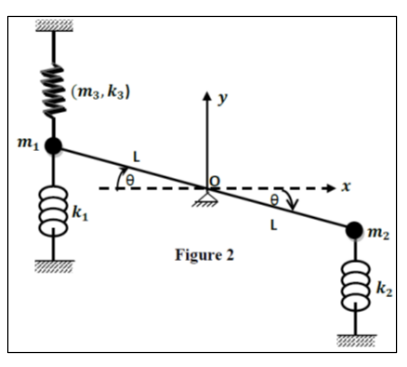
\includegraphics[width=0.7\textwidth]{images/vibrations/vib-001-000.png}
\caption{Système masse-ressort horizontal : schéma.}
\end{figure}

\begin{figure}[H]
\centering
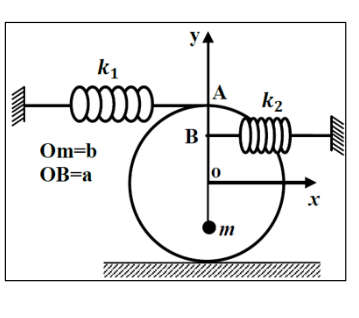
\includegraphics[width=0.7\textwidth]{images/vibrations/vib-002-004.png}
\caption{Poulie avec ressort et masse.}
\end{figure}

\begin{figure}[H]
\centering
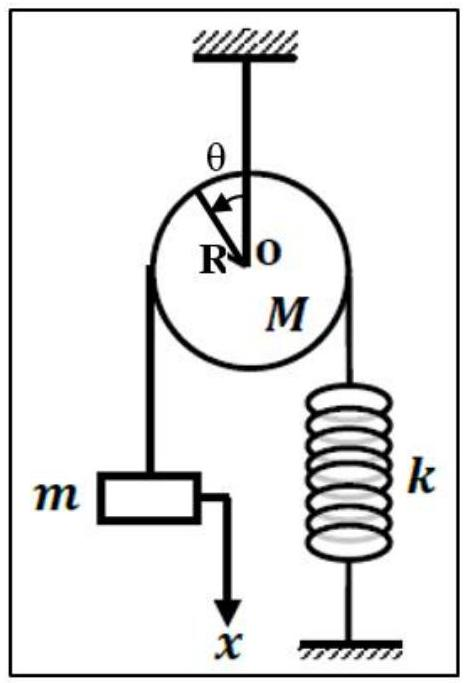
\includegraphics[width=0.7\textwidth]{images/vibrations/vib-004-007.png}
\caption{Oscillateur amorti : régime sous-critique.}
\end{figure}

\begin{figure}[H]
\centering
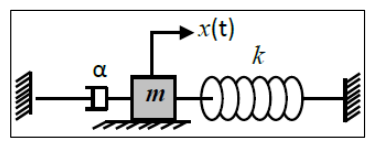
\includegraphics[width=0.7\textwidth]{images/vibrations/vib-006-008.png}
\caption{Résonance d'un oscillateur forcé.}
\end{figure}

\begin{figure}[H]
\centering
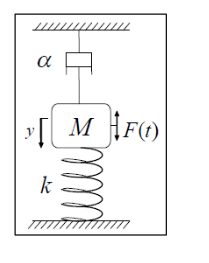
\includegraphics[width=0.7\textwidth]{images/vibrations/vib-009-014.png}
\caption{Deux masses couplées par un ressort.}
\end{figure}

\begin{figure}[H]
\centering
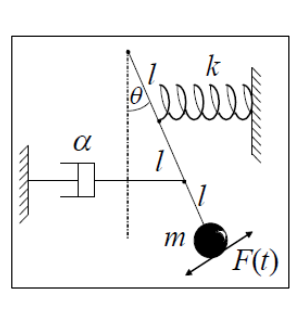
\includegraphics[width=0.7\textwidth]{images/vibrations/vib-011-016.png}
\caption{Modes normaux d'un système à 2 ddl.}
\end{figure}

\begin{figure}[H]
\centering
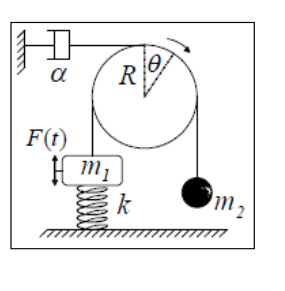
\includegraphics[width=0.7\textwidth]{images/vibrations/vib-013-018.png}
\caption{Barre oscillante avec amortissement.}
\end{figure}

\begin{figure}[H]
\centering
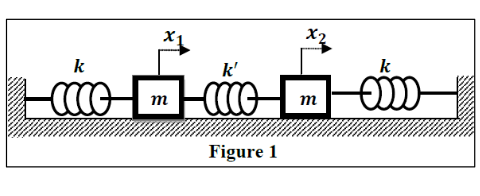
\includegraphics[width=0.7\textwidth]{images/vibrations/vib-015-020.png}
\caption{Ondes progressives sur une corde.}
\end{figure}

\begin{figure}[H]
\centering
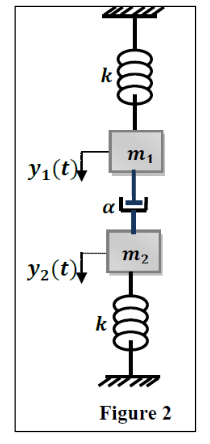
\includegraphics[width=0.7\textwidth]{images/vibrations/vib-017-022.png}
\caption{Ondes stationnaires : n\oe{}uds et ventres.}
\end{figure}

\begin{figure}[H]
\centering
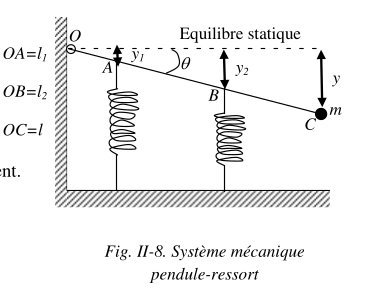
\includegraphics[width=0.7\textwidth]{images/vibrations/vib-018-024.png}
\caption{Battements : somme de deux oscillations.}
\end{figure}

\begin{figure}[H]
\centering

\includegraphics[width=0.7\textwidth]{images/vibrations/vib-001-001.png}
\caption{Pendule simple : mise en équation.}
\end{figure}

\begin{figure}[H]
\centering
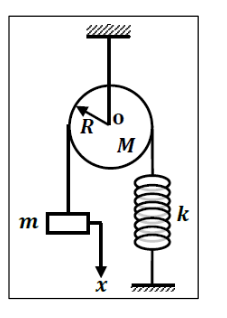
\includegraphics[width=0.7\textwidth]{images/vibrations/vib-001-002.png}
\caption{Pendule élastique vertical.}
\end{figure}

\begin{figure}[H]
\centering

\includegraphics[width=0.7\textwidth]{images/vibrations/vib-002-005.png}
\caption{Oscillateur amorti : régime apériodique.}
\end{figure}

\begin{figure}[H]
\centering

\includegraphics[width=0.7\textwidth]{images/vibrations/vib-006-009.png}
\caption{Résonance en force d'un oscillateur harmonique.}
\end{figure}

\begin{figure}[H]
\centering
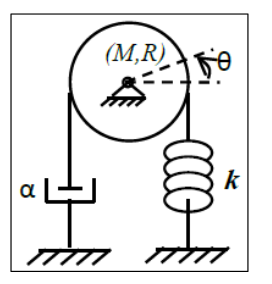
\includegraphics[width=0.7\textwidth]{images/vibrations/vib-006-010.png}
\caption{Bande passante et facteur de qualité.}
\end{figure}

\begin{figure}[H]
\centering

\includegraphics[width=0.7\textwidth]{images/vibrations/vib-006-011.png}
\caption{Oscillations couplées : modes normaux.}
\end{figure}

\begin{figure}[H]
\centering

\includegraphics[width=0.7\textwidth]{images/vibrations/vib-011-017.png}
\caption{Couplage par ressort entre deux masses.}
\end{figure}

\begin{figure}[H]
\centering

\includegraphics[width=0.7\textwidth]{images/vibrations/vib-013-019.png}
\caption{Système à trois masses couplées.}
\end{figure}

\begin{figure}[H]
\centering

\includegraphics[width=0.7\textwidth]{images/vibrations/vib-015-021.png}
\caption{Corde vibrante : équation d'Alembert.}
\end{figure}

\begin{figure}[H]
\centering

\includegraphics[width=0.7\textwidth]{images/vibrations/vib-017-023.png}
\caption{Mode fondamental et harmoniques de corde.}
\end{figure}

\begin{figure}[H]
\centering

\includegraphics[width=0.7\textwidth]{images/vibrations/vib-018-025.png}
\caption{Analyse spectrale d'un signal en battements.}
\end{figure}

\ifdefined\inMainDoc\else\end{document}\fi


\end{document}
